% Options for packages loaded elsewhere
\PassOptionsToPackage{unicode}{hyperref}
\PassOptionsToPackage{hyphens}{url}
%
\documentclass[
  letterpaper,
]{scrbook}
\usepackage{amsmath,amssymb}
\usepackage{lmodern}
\usepackage{iftex}
\ifPDFTeX
  \usepackage[T1]{fontenc}
  \usepackage[utf8]{inputenc}
  \usepackage{textcomp} % provide euro and other symbols
\else % if luatex or xetex
  \usepackage{unicode-math}
  \defaultfontfeatures{Scale=MatchLowercase}
  \defaultfontfeatures[\rmfamily]{Ligatures=TeX,Scale=1}
\fi
% Use upquote if available, for straight quotes in verbatim environments
\IfFileExists{upquote.sty}{\usepackage{upquote}}{}
\IfFileExists{microtype.sty}{% use microtype if available
  \usepackage[]{microtype}
  \UseMicrotypeSet[protrusion]{basicmath} % disable protrusion for tt fonts
}{}
\makeatletter
\@ifundefined{KOMAClassName}{% if non-KOMA class
  \IfFileExists{parskip.sty}{%
    \usepackage{parskip}
  }{% else
    \setlength{\parindent}{0pt}
    \setlength{\parskip}{6pt plus 2pt minus 1pt}}
}{% if KOMA class
  \KOMAoptions{parskip=half}}
\makeatother
\usepackage{xcolor}
\usepackage{longtable,booktabs,array}
\usepackage{calc} % for calculating minipage widths
% Correct order of tables after \paragraph or \subparagraph
\usepackage{etoolbox}
\makeatletter
\patchcmd\longtable{\par}{\if@noskipsec\mbox{}\fi\par}{}{}
\makeatother
% Allow footnotes in longtable head/foot
\IfFileExists{footnotehyper.sty}{\usepackage{footnotehyper}}{\usepackage{footnote}}
\makesavenoteenv{longtable}
\usepackage{graphicx}
\makeatletter
\def\maxwidth{\ifdim\Gin@nat@width>\linewidth\linewidth\else\Gin@nat@width\fi}
\def\maxheight{\ifdim\Gin@nat@height>\textheight\textheight\else\Gin@nat@height\fi}
\makeatother
% Scale images if necessary, so that they will not overflow the page
% margins by default, and it is still possible to overwrite the defaults
% using explicit options in \includegraphics[width, height, ...]{}
\setkeys{Gin}{width=\maxwidth,height=\maxheight,keepaspectratio}
% Set default figure placement to htbp
\makeatletter
\def\fps@figure{htbp}
\makeatother
\setlength{\emergencystretch}{3em} % prevent overfull lines
\providecommand{\tightlist}{%
  \setlength{\itemsep}{0pt}\setlength{\parskip}{0pt}}
\setcounter{secnumdepth}{5}
% Make \paragraph and \subparagraph free-standing
\ifx\paragraph\undefined\else
  \let\oldparagraph\paragraph
  \renewcommand{\paragraph}[1]{\oldparagraph{#1}\mbox{}}
\fi
\ifx\subparagraph\undefined\else
  \let\oldsubparagraph\subparagraph
  \renewcommand{\subparagraph}[1]{\oldsubparagraph{#1}\mbox{}}
\fi
\RedeclareSectionCommand[beforeskip=-2.5ex plus -1ex minus -.2ex,afterskip=0.3ex plus -.2ex]{section}
\RedeclareSectionCommand[tocnumwidth=3em]{section}
\usepackage[top=0.5in, left=0.5in, right=0.5in, bottom=1in]{geometry}
\bibliographystyle{catalog}
\usepackage{makeidx}
\makeindex
\renewcommand\toprule[2]\relax
\renewcommand\bottomrule[2]\relax
\usepackage{fancyhdr}
\lfoot{\textit{Coe College (2022-2023)}}
\renewcommand{\part}[1]{\addcontentsline{toc}{part}{#1}}
\makeatletter
\@ifpackageloaded{bookmark}{}{\usepackage{bookmark}}
\makeatother
\makeatletter
\@ifpackageloaded{caption}{}{\usepackage{caption}}
\AtBeginDocument{%
\ifdefined\contentsname
  \renewcommand*\contentsname{Table of contents}
\else
  \newcommand\contentsname{Table of contents}
\fi
\ifdefined\listfigurename
  \renewcommand*\listfigurename{List of Figures}
\else
  \newcommand\listfigurename{List of Figures}
\fi
\ifdefined\listtablename
  \renewcommand*\listtablename{List of Tables}
\else
  \newcommand\listtablename{List of Tables}
\fi
\ifdefined\figurename
  \renewcommand*\figurename{Figure}
\else
  \newcommand\figurename{Figure}
\fi
\ifdefined\tablename
  \renewcommand*\tablename{Table}
\else
  \newcommand\tablename{Table}
\fi
}
\@ifpackageloaded{float}{}{\usepackage{float}}
\floatstyle{ruled}
\@ifundefined{c@chapter}{\newfloat{codelisting}{h}{lop}}{\newfloat{codelisting}{h}{lop}[chapter]}
\floatname{codelisting}{Listing}
\newcommand*\listoflistings{\listof{codelisting}{List of Listings}}
\makeatother
\makeatletter
\makeatother
\makeatletter
\@ifpackageloaded{caption}{}{\usepackage{caption}}
\@ifpackageloaded{subcaption}{}{\usepackage{subcaption}}
\makeatother
\ifLuaTeX
  \usepackage{selnolig}  % disable illegal ligatures
\fi
\IfFileExists{bookmark.sty}{\usepackage{bookmark}}{\usepackage{hyperref}}
\IfFileExists{xurl.sty}{\usepackage{xurl}}{} % add URL line breaks if available
\urlstyle{same} % disable monospaced font for URLs
\hypersetup{
  pdftitle={Course Catalog 2022-2023},
  hidelinks,
  pdfcreator={LaTeX via pandoc}}

\title{Course Catalog 2022-2023}
\author{}
\date{2022-08-01}

\begin{document}
\frontmatter
\maketitle

\renewcommand*\contentsname{Table of contents}
{
\setcounter{tocdepth}{1}
\tableofcontents
}
\mainmatter
\bookmarksetup{startatroot}

\chapter*{PREFACE}\label{preface}

\markboth{PREFACE}{PREFACE}

\section*{Non-Discrimination}\label{non-discrimination}

\markright{Non-Discrimination}

Coe College does not discriminate on the basis of race, color,
ethnicity, age, religion, national origin, sexual orientation, gender
identity, sex, marital status, disability, or status as a U.S. Veteran.
All students have equal access to the facilities, financial aid, and
programs of the College.

\section*{Higher Education Opportunity Act
(HEOA)}\label{higher-education-opportunity-act-heoa}

\markright{Higher Education Opportunity Act (HEOA)}

The College complies with Readmission Requirements for Service Members
as outlined in the Higher Education Opportunity Act section 487. This
applies to active duty in the Armed Forces, whether voluntary or
involuntary, including service as a member of the National Guard or
Reserve, for a period of more than 30 days under a call or order to
active duty.

The HEOA provides that a prompt readmission of a previously enrolled or
admitted student may not be denied to a service member of the uniformed
services for reasons relating to that service.~ In addition, a student
who is readmitted under this section must be readmitted with the same
academic status as the student had when they attended the college.

\section*{Equal Opportunity in
Employment}\label{equal-opportunity-in-employment}

\markright{Equal Opportunity in Employment}

Coe College is an equal opportunity employer in the recruitment and
hiring of faculty and staff.

\section*{Family Educational Rights and Privacy Act
(FERPA)}\label{family-educational-rights-and-privacy-act-ferpa}

\markright{Family Educational Rights and Privacy Act (FERPA)}

The provisions of the Family Educational Rights and Privacy Act (FERPA)
prohibit the College from releasing grades or other information about
academic standing to parents unless the student has released such
information in writing. Further information concerning Coe College
procedures in compliance with FERPA is available in the Office of the
Registrar and included on p.~68 of this catalog.

\section*{Solomon Amendment of 1997}\label{solomon-amendment-of-1997}

\markright{Solomon Amendment of 1997}

Pursuant to the regulations of the Solomon Amendment of 1997, Coe
College is required to make student recruiting information available to
military recruiters who request it.

\section*{Reservation of the Right to
Modify}\label{reservation-of-the-right-to-modify}

\markright{Reservation of the Right to Modify}

The provisions of this catalog are to be considered directive in
character and not as an irrevocable contract between the student and the
College. The College reserves the right to make changes that seem
necessary or desirable, including course and program cancellations.
Responsibility for understanding and meeting graduation requirements as
stated in the Coe College Catalog rests entirely with the student.
Faculty advisors and the Registrar will assist in every way possible.

\part{INTRODUCTORY RESOURCES}

\chapter{MISSION STATEMENT OF THE
COLLEGE}\label{sec-mission-statement-of-college}

\begin{center}

\includegraphics{catalog_sections/graphics/coe_bell.png}
\end{center}

\index{Mission Statement}

Coe College is a national, residential liberal arts college offering a
broad array of programs in the arts, sciences and professions. Our
mission is to prepare students for meaningful lives and fulfilling
careers in a diverse, interconnected world. Coe's success will be judged
by the success of our graduates.

\emph{Coe College admits students without regard to sex, race, creed,
color, handicap, sexual orientation, national, or ethnic origin. All
students have equal access to the facilities, financial aid, and
programs of the College.}

\chapter{FAST FACTS}\label{sec-fast-facts}

\textbf{COE COLLEGE} is a private, four-year co-educational liberal arts
college that was founded in 1851 and is historically affiliated with the
Presbyterian Church (U.S.A.), yet is ecumenical in practice and outlook.

\section{LOCATION}\label{location}

Coe is located just 225 miles west of Chicago in Iowa's second largest
city, Cedar Rapids (metropolitan population 175,000). The city is easily
accessible by the interstate highway system, bus services and several
airlines.

\section{CAMPUS}\label{campus}

Situated on 65 acres in the center of the metropolitan area, the campus
is urban but enclosed, with 30 buildings occupying an attractive
landscape.

\section{ENROLLMENT}\label{enrollment}

The student body of approximately 1,400 students represents most states
and around 15 foreign countries. All students are required to live on
campus unless they are residents of Cedar Rapids.

\section{LIBRARY}\label{library}

Stewart Memorial Library is in the very center of the main campus. It
contains over 500,000 volumes and 16,000 pieces of media, and subscribes
to 3,500 print and online periodical subscriptions providing access to
over 100 databases. Coe's library offers students a variety of research
assistance, study areas, a small theater, preview room, a media editing
room, and a 3D printer and laser cutter. The Library houses the Learning
Commons and the College's permanent art collection.

\section{ACCREDITATION}\label{accreditation}

Coe College is accredited by the Higher Learning Commission
(hlcomission.org), an institutional accreditation agency recognized by
the U.S. Department of Education. Coe College's Bachelor of Music
program is accredited by the National Association of Schools of Music;
its education program is accredited by the Iowa Department of Education,
and its Bachelor of Science in Nursing is accredited by the Commission
on Collegiate Nursing Education
(http://aacn.nche.edu/ccne-accreditation).~ Coe College's chemistry
program is certified by the American Chemical Society.~ Copies of
accrediting and approval statements are available online at
https://www.coe.edu/why-coe/consumer-information.

\section{MEMBERSHIPS}\label{memberships}

Coe is a charter member of the Associated Colleges of the Midwest, whose
other members are: Beloit, Carleton, Colorado, Cornell, Grinnell, Knox,
Lake Forest, Lawrence, Luther, Macalester, Monmouth, Ripon, and
St.~Olaf. Other memberships include: Phi Beta Kappa, Phi Kappa Phi, the
National Association of Independent Colleges and Universities, the
American Association of Colleges and Universities, Council on
Undergraduate Research, the Association of Presbyterian Colleges and
Universities, the American Rivers Conference, and the National
Collegiate Athletic Association.

\section{ACADEMIC PROGRAM}\label{academic-program}

Academic areas of study are offered in managerial or public accounting,
African American studies, art, art history, Asian studies, biology,
business administration, chemistry, communication studies, computer
science, creative writing, data science, economics, elementary
education, English, film studies, French \& francophone studies,
interdisciplinary French \& francophone studies, general science,
history, international business, international economics, international
studies, kinesiology, literature, mathematics, music (B.A. or B.M.),
nursing (B.S.N.), philosophy, physics, political science, psychology,
religion, social \& criminal justice, sociology, Spanish, Spanish
studies, theatre arts, and writing. Interdisciplinary and/or collateral
majors are also available in biochemistry, environmental science,
environmental studies, molecular biology, neuroscience, organizational
science, and public relations. Coe also offers certificate programs in
primary and secondary education.

\section{EXTRA-CURRICULAR ACTIVITIES}\label{extra-curricular-activities}

Students can participate in 11 men's and 11 women's NCAA Division III
varsity athletic teams, 5 coed varsity athletic teams, 8 club sports, 10
nationally affiliated men's and women's social fraternities, and 65
student organizations including but not limited to student government,
newspaper, intramural sports, departmental clubs, and residence hall
activities. Various vocal and instrumental ensembles are available for
course credit.

\section{FINANCIAL ASSISTANCE}\label{financial-assistance}

Coe College is committed to assisting those families in need of
financial assistance. The average aid package for incoming students
enrolled during the 2021--2022 academic year totaled more than \$48,000.
The total cost of full-time tuition, room, board, and activity fee for
the 2021--2022 academic year is \$59,324.

\section{HISTORY OF COE COLLEGE}\label{sec-history-of-coe-college}

Coe College claims the shortest name of any American institution of
higher education, but the school has actually carried five titles
through its history. When the Rev.~Williston Jones founded the college
in 1851, he called it The School for the Prophets. Cedar Rapids' first
resident minister opened the parlor of his home to a group of young men
with the goal of educating them for the ministry to serve churches in
the Midwest. Two years later, while Jones was canvassing churches in the
East for money to send three of his students to Eastern seminaries, a
Catskills farmer named Daniel Coe stepped forward with a pledge of
\$1,500 and urged Jones to start his own college in the frontier town of
Cedar Rapids. Legend has it that the \$1,500 raised by Coe was brought
west from New York, sewn into the petticoat of a lady visitor traveling
by stagecoach to Iowa. Coe gave this generous gift with the stipulation
that the proposed institute should be ``made available for the education
of females as well as males.'' Accordingly, Coe was coeducational from
its founding.

With Jones' blessing, the Cedar Rapids Collegiate Institute was
incorporated in 1853 by a group of Cedar Rapids leaders chaired by Judge
George Greene. They used Daniel Coe's money to purchase two downtown
lots for the school and 80 acres of farmland on what was then the edge
of town. The farm evolved into today's campus. In 1868, in a failed
attempt to secure the Lewis Parsons estate, the trustees renamed the
school Parsons Seminary. After a period of severe financial
difficulties, the institution was reestablished in honor of its original
benefactor as the Coe Collegiate Institute in 1875.

T.M Sinclair, founder of the Sinclair Meat Packing Company, played the
key financial role in the final step toward the firm establishment of
Coe College. Sinclair liquidated all the debt from Parsons Seminary and
the Cedar Rapids Collegiate Institute. The Sinclair gift made it
practical for the property of the Coe Collegiate Institute---including
the original land paid for by Daniel Coe---to be transferred to Coe
College with the Iowa Presbyterian Synod to assume major responsibility
for the institution. Coe College has operated continuously since its
incorporation under that name on Feb.~2, 1881. From the first, the
College was committed to intellectual excellence. It has continued in
this tradition ever since.

The compact campus on the east edge of Cedar Rapids grew with many
building projects in its early years, including Old Main (1868),
Williston Hall (1881), Marshall Hall (1900), the first gymnasium (1904),
and the first T.M. Sinclair Memorial Chapel (1911). In 1907, Coe earned
accreditation from the North Central Association of Colleges and
Universities. Over the decades, Coe's reputation as a superior liberal
arts college has continued to grow. One recognition of this came in
1949, when Coe was granted a Phi Beta Kappa chapter, a distinction
reserved for about 10\% of American colleges and universities.

Central to the educational philosophy of Coe College is the belief that
a liberal arts education is the best preparation for life. Students have
the opportunity to experience a variety of subjects outside their
respective programs of study. Coe offers more than 40 areas of study
that cover a range of fields. The College awards the following
undergraduate degrees: Bachelor of Arts (B.A.), Bachelor of Music
(B.M.), and Bachelor of Science in Nursing (B.S.N.).

There are a number of factors that contribute to Coe College's strong
academic quality. The key to Coe's tradition of excellence in academic
quality relates directly to small class sizes and the interest shown by
professors to make learning a personalized experience. At Coe, the
average class size is 16, and the student-faculty ratio is 11:1. Classes
are taught by our involved and committed faculty, 91\% of whom hold the
highest degree in their field. This means classes are taught by
experienced professionals who have in-depth knowledge of their subjects.
To provide students with a well-rounded experience and solid preparation
for the future, Coe offers, along with quality instruction from superb
faculty, an abundance of out-of-class opportunities which include
student-faculty collaborative research, honors projects, service
learning, and internships. Within one year of graduation, according to
the annual survey results from the Center for Creativity and Careers,
98\% of Coe graduates are engaged in post-graduate activity such as
employment, graduate school, military, or travel/adventure.

With the addition of the east campus, Coe has nearly doubled in size
since 1989. New facilities on the east side of College Drive include
Athletic Recreation Center (2017), Clark Racquet Center and athletic
fields (1989), Clark Alumni House (1993), Nassif House (1999), and four
student apartment buildings (Morris House and Schlarbaum House in 2000,
Brandt House and Spivey House in 2002). McCabe Hall (2005), named in
honor of former Coe President Joseph E. McCabe, houses the offices of
the president, provost, advancement and alumni relations, and The Center
for Creativity, Careers and Community (C3) making way for the remodeling
of Coe's oldest building, Stuart Hall, and the first significant
addition of classroom space since Peterson Hall was built in the 1960s.
In 2012 and 2013, Peterson Hall of Science was completely renovated to
support Coe's science programs. To further enhance the campus
environment, Coe completed the largest capital project in its history in
2017. Make Your Move -- the Campaign for Eby and Hickok -- included \$24
million in essential enhancements, including an Athletic and Recreation
Complex project as well as the renovation and expansion of Hickok Hall,
one of the College's main academic buildings. The result is vastly
improved academic, recreational, wellness and competition facilities to
benefit future generations of students.

\part{ACADEMIC RESOURCES}

\chapter{2022--2023 ACADEMIC CALENDAR}\label{sec-academic-calenar}

\section{FALL TERM 2022}\label{fall-term-2022}

\begin{longtable}[]{@{}
  >{\raggedright\arraybackslash}p{(\columnwidth - 2\tabcolsep) * \real{0.3333}}
  >{\raggedleft\arraybackslash}p{(\columnwidth - 2\tabcolsep) * \real{0.6667}}@{}}
\toprule\noalign{}
\endhead
\bottomrule\noalign{}
\endlastfoot
Tues, August 23 & Open Registration \\
Wed, August 24 & Classes Begin \\
Tues, August 30 & Last Day to Add or Drop a Full-Term, or 1st Half-Term
Course without a W \\
Fri, September 2 & Census Date, Attendance Due on My.Coe \\
Mon, September 5 & No Classes (Holiday) Labor Day \\
Fri, September 9 & Date of Record \\
Thurs, September 22 & Last Day to Withdraw \&/ or Change Method of
Grading for First-Half Courses \\
Mon--Tues, October 10--11 & Fall Term Break \\
Thurs--Sat, October 13--15 & Homecoming \\
Mon, October 17 & Mid-Term Progress Report Due on My.Coe (11:59 PM) \\
Mon, October 17 & Begin Second-Half Term Courses \\
Fri, October 21 & May Term deposit and registration due \\
Fri, October 21 & Last Day to Add or Drop a Second-Half Term Course
without a W \\
Mon, October 24-Fri, November 11 & Advising Season \\
Fri, October 28 & Last Day to Withdraw \&/or Change Method of Grading
for Full-Term Courses \\
Mon--Fri, November 14--18 & Registration for Spring Term 2023 \\
Tues, November 15 & Last Day to Withdraw \&/or Change Method of Grading
for Second-Half Courses \\
Mon--Fri, November 21--25 & No Classes (Holiday) Thanksgiving Recess \\
Thurs, December 1 & Open Online Registration until Last Day of Finals \\
Fri, December 2 & Last Day of Fall Term Classes \\
Sat, December 3 & Reading Day \\
Mon--Thurs, December 5--8 & Final Exams \\
Wed, December 14 & Final Grades and Attendance are Due from the Faculty
on My.Coe (11:59 PM) \\
\end{longtable}

\section{SPRING TERM 2023}\label{spring-term-2023}

\begin{longtable}[]{@{}
  >{\raggedright\arraybackslash}p{(\columnwidth - 2\tabcolsep) * \real{0.3333}}
  >{\raggedleft\arraybackslash}p{(\columnwidth - 2\tabcolsep) * \real{0.6667}}@{}}
\toprule\noalign{}
\endhead
\bottomrule\noalign{}
\endlastfoot
Wed, January 11 & Classes Begin \\
Mon, January 16 & No Day Classes (Holiday) Martin Luther King Jr.~Day \\
Wed, January 18 & Last Day to Add or Drop a Full-Term or 1st Half-Term
Course without a W \\
Fri, January 20 & Census Date, Attendance Due on My.Coe \\
Thurs, January 26 & Date of Record Mon, February 6 \\
Mon, February 6 & Last Day to Withdraw \&/or Change Method of Grading
for First-Half Courses \\
Mon, March 6 & Begin Second-Half Term Courses \\
Tues, March 7 & Mid-Term Progress Report Due Online (11:59 PM) \\
Fri, March 10 & Last Day to Add or Drop a Second-Half Term Course
without a W \\
Mon--Fri, March 13--17 & Spring Term Recess (Starting after Class on
Friday, March 10) \\
Mon--Fri, March 20--April 7 & Advising Season Thurs, March 30 \\
Thurs, March 30 & Last Day to Withdraw \&/or Change Method of Grading
for Full-Term Courses \\
Mon--Fri, April 10--14 & Registration for Fall Term 2023 \\
Mon, April 10 & Summer Registration Opens \\
Tues, April 11 & Last Day to Withdraw \&/or Change Method of Grading for
Second-Half Courses \\
Wed, April 12 & Student Research Symposium ** No Day Classes ** Evening
Classes Will Meet \\
Fri, April 28 & Last Day of Spring Term Classes \\
Sat, April 29 & Reading Day \\
Mon--Thurs, May 1--4 & Final Exams \\
Sat, May 6 & Honors Convocation / Baccalaureate \\
Sun, May 7 & Commencement \\
Tues, May 9 & Final Grades and Attendance are Due for Non-Graduating
Students on My.Coe (11:59 PM) \\
\end{longtable}

\section{MAY TERM 2023}\label{may-term-2023}

\begin{longtable}[]{@{}
  >{\raggedright\arraybackslash}p{(\columnwidth - 2\tabcolsep) * \real{0.3333}}
  >{\raggedleft\arraybackslash}p{(\columnwidth - 2\tabcolsep) * \real{0.6667}}@{}}
\toprule\noalign{}
\endhead
\bottomrule\noalign{}
\endlastfoot
Wed, May 10 & Classes Begin \\
Fri, May 12 & Last Day to Add or Drop a Course Without a W \\
Mon, May 15 & Attendance Due Online; Last Day to Change Method of
Grading for May Term \\
Wed, May 17 & Last Day to Withdraw from May Term Courses \\
Fri--Sat, May 19--20 & Meeting of the Board of Trustees \\
Mon, May 29 & No Classes (Holiday) Memorial Day \\
Fri, June 2 & Last Day of May Term Classes \\
Sat, June 3 & Residence Halls Close \\
Sun, June 4 & Final Grades and Attendance for May Term Due on My.Coe
(11:59 PM) \\
\end{longtable}

\section{SUMMER TERM 2023*}\label{summer-term-2023}

\begin{longtable}[]{@{}
  >{\raggedright\arraybackslash}p{(\columnwidth - 2\tabcolsep) * \real{0.3333}}
  >{\raggedleft\arraybackslash}p{(\columnwidth - 2\tabcolsep) * \real{0.6667}}@{}}
\toprule\noalign{}
\endhead
\bottomrule\noalign{}
\endlastfoot
Mon, June 5 & Classes Begin \\
Fri, June 9 & Last Day to Add or Drop a Full-Term Course Without a W \\
Mon, June 19 & No Classes (Holiday) Juneteenth \\
Fri, June 23 & Last Day to Change Method of Grading \&/or Withdraw from
Block A Courses \\
Tues, July 4 & No Classes (Holiday) Independence Day \\
Fri, July 7 & Last Day of Block A Courses \\
Mon, July 10 & Classes Begin: Block B Courses \\
Tues, July 11 & Mid-Term Progress Report Due Online (11:59 PM); Block A
Final Grades Due \\
Fri, July 14 & Last Day to Add or Drop a Course Without a W for Block B
Courses \\
Mon, July 17 & Last Day to Change Method of Grading \&/or Withdraw from
Full Term Courses \\
Tues, July 25 & Last Day to Change Method of Grading \&/or Withdraw from
Block B Courses \\
Fri, August 11 & Last Day of Term Classes: Block B and Full-Term
Courses \\
Tues, August 15 & Final Grades and Attendance Due (Block B and
Full-Term) on My.Coe (11:59 PM) \\
\end{longtable}

*Courses taught at the Wilderness Field Station are subject to the broad
dates of the summer, but will provide a specific add/drop and withdraw
calendar to students at the time of application.

\chapter{THE ACADEMIC CALENDAR}\label{the-academic-calendar}

The academic year consists of three terms (see Academic Calendar,
\textbf{?@sec-academic-calendar}). Students normally take four course
credits in the Fall Term and four course credits in the Spring Term.
Thus, eight course credits are completed in an academic year. During
optional May Term, students may enroll for up to one course credit in
one of the limited selection of courses. Summer term is limited in scope
and is not considered a regular term. (The maximum course load is
described in Course Load, Section~\ref{sec-course-load}).

\chapter{MAY TERM (OPTIONAL)}\label{may-term-optional}

Students may enroll for up to one course credit during May Term in one
of the limited selection of courses. All May Term courses require
consent of instructor prior to registration. May Term courses are
designed to meet at least two of the following shared learning outcomes:

\begin{itemize}
\tightlist
\item
  Evaluate and engage with complex interdependent systems and
  demonstrate understanding across diverse contexts.
\item
  Critically describe and break apart issues or problems through
  systematic analysis and illustrate logic for conclusions.
\item
  Engage with experiential learning practices such as learning by doing,
  while utilizing abilities to think critically, problem solve and make
  connections between knowledge gained in the classroom and experience
  beyond.
\end{itemize}

May Term courses are expected to have the same amount of contact time
and academic rigor per course credit as courses which meet over a Fall
or Spring Term.~ For every 1 course credit of May term students are
expected to complete 140 hours of work. Such contact time includes class
meetings, lectures by the instructor, supervised course related
activities and independent out of class activities.~ Off-campus May Term
courses at an off-campus location provide certain educational benefits
through site visits, guest lectures, etc., that also contribute to the
contact time for the course.

\chapter{COE PLAN}\label{sec-coe-plan}

Coe College's requirements for graduation, commonly known as the
\emph{Coe Plan} were developed with the following outcomes in mind:

\begin{itemize}
\tightlist
\item
  Creation of a bridge from high school to Coe College that helps
  students understand the importance of a liberal arts education, the
  ways to develop the skills needed by any learner, and the
  opportunities they will have by going to Coe College.
\item
  Development of required curriculum that exposes the students to ways
  of learning in various contexts, big ideas in a myriad of disciplines,
  ways of being and understanding of cultures around the world, and
  processes to develop the skills needed by any learner.
\item
  Creation of a bridge from Coe College to life after Coe.
\end{itemize}

These outcomes are met through the College's First-Year Experience,
General Education program, Writing Emphasis courses, and the College's
Practicum experiences and areas of study, described in this section of
the Catalog.

\chapter{GRADUATION REQUIREMENTS}\label{sec-graduation-requirements}

All students who graduate from Coe College must complete at least one
major and earn at least 32 course credits (cc) with grades leading to a
cumulative grade point average (GPA) of 2.0 or higher. (\emph{The course
is the unit of academic credit.}) Courses are one credit unless
otherwise indicated. Students are expected to complete 180 hours of work
to earn one course credit, although class times vary from course to
course. Other institutions may convert Coe credit to their system by
considering one course credit to be 6 quarter hours, or 4 semester
hours.) No more than a total of two course credits from courses which
are less than 0.5 credit can be used to meet the 32-credit graduation
requirement. No more than eight course credits earned of Advanced
Placement or International Baccalaureate credit can be used to satisfy
this requirement.

Students must meet one of the following requirements:

\begin{itemize}
\tightlist
\item
  Complete at least the final academic year of required courses
  registered through Coe.
\item
  Earn a total of 16 course credits or the equivalent at Coe. The last
  eight course credits needed for graduation must include at least four
  earned at Coe. Approved off-campus study programs and internships can
  be used to fulfill this requirement.
\end{itemize}

A student may be simultaneously awarded two degrees (B.A., B.M., B.S.N.)
after satisfactorily completing 40 course credits and the requirements
for both degrees. However, a simultaneous Bachelor of Music plus a
Bachelor of Arts with a music major is not permitted.

In addition, students must fulfill the requirements of the First-Year
Experience, General Education, Writing Emphasis, and Practicum.

To participate in Commencement exercises, students must submit a
completed Intent to Graduate form to the Office of the Registrar,
preferably three terms prior to Commencement.

\section{Second Baccalaureate
Degree}\label{sec-second-baccalaureate-degree}

A student who holds a baccalaureate degree from another institution may
earn a second baccalaureate degree at Coe, if the following criteria are
met:

\begin{itemize}
\tightlist
\item
  The first degree must be from a regionally accredited institution as
  recognized by the US Department of Education, or another appropriate
  accrediting body.
\item
  The first degree must be completed (not in progress) before beginning
  the second degree at Coe.
\end{itemize}

Students accepted at Coe to pursue a second degree are granted a maximum
of 24 course credits in transfer credit towards the 32 course credits
required for graduation. To graduate, at least eight course credits must
be earned at Coe College and all requirements for the major area of
study must be met with at least 40\% of the major course credits taken
at Coe. Students must earn a cumulative GPA of at least 2.0 as well as
meet any GPA or grade requirements in their area of study.

Second baccalaureate students are exempt from the following
requirements: first-year experience, general education, writing
emphasis, and practicum. They are not eligible to graduate with Latin
Honors or for induction in Phi Beta Kappa or Phi Kappa Phi.

\section{Transfer Student
Information}\label{transfer-student-information}

To honor its mission and to preserve its academic integrity as a liberal
arts institution, the College accepts a course in transfer if that
course meets the spirit of the College's mission and is from a
regionally accredited institution. This section includes information, in
addition to that included in the section, Graduation Requirements (see
Chapter~\ref{sec-graduation-requirements}), germane to students who are
transferring to Coe College from another college or university.

Courses transferred to Coe can, as approved by the Registrar, fulfill
some graduation requirements. From institutions on a semester hour
system (at Coe, 1 course credit = 4 semester hours), only courses with
three or more semester hours can be used to fulfill any major or general
education requirements. From institutions on other than a semester hour
system, only courses equivalent to at least 0.75 course credits can be
used to fulfill any major or general education requirement. In some
cases, in consultation with the Registrar, multiple courses within the
same field may be used to fulfill one requirement.

Transfer credits earned after high-school graduation and before Coe
matriculation count towards the eight term, full-time residence
requirement (see Section~\ref{sec-full-time-residence-requirements}).
Full-time enrollment may include participation in Coe College exchange
programs, ACM off-campus study programs, and other approved off-campus
study programs.

All students must complete at Coe at least 40\% of the total course
credits required for each declared major or minor or three course
credits, whichever is greater. In addition to completing at least one
major area of study, transfer students must abide with the following to
complete the requirements for graduation:

\begin{itemize}
\tightlist
\item
  First-Year Experience. Transfer students are not required to fulfill
  the requirements of the First-Year Experience, if they have completed
  at least one full-time college term since graduation from high school.
\item
  Writing Emphasis. (See Writing Emphasis Courses,
  Chapter~\ref{sec-writing-emphasis-courses}).
\item
  General Education. Requirements include \textbf{Liberal Arts}
  selections in the four divisional areas (Natural and Mathematical
  Sciences, Social Sciences, Humanities, Fine Arts) and \textbf{Diverse
  Cultural Perspectives} courses. Any courses accepted in transfer for
  at least 0.75 course credit that fit the criteria of the Liberal Arts
  and/or Diverse Cultural Perspectives core groups can be applied
  towards the general education requirements as determined by the
  Registrar. Advanced Placement and International Baccalaureate courses
  may not be used to meet any part of the General Education
  requirements.
\item
  Academic Practicum. Transfer students are required to fulfill this
  requirement.
\end{itemize}

\chapter{AREAS OF STUDY}\label{sec-areas-of-study}

The three undergraduate degrees have areas of study associated with
them. The Bachelor of Science in Nursing's area of study is nursing; the
Bachelor of Music's areas of study are performance, composition, and
education. The Bachelor of Arts' areas of study, commonly referred to as
majors, are listed below.

Students should declare an area of study by the end of their sophomore
year. All students must earn at least a 2.00 GPA in courses required to
complete their areas of study, as well as meet specific requirements set
forth for the areaof study.

\begin{itemize}
\tightlist
\item
  Accounting, Managerial
\item
  Accounting, Public
\item
  African American Studies
\item
  Art
\item
  Art History
\item
  Asian Studies
\item
  Biology
\item
  Business Administration
\item
  Chemistry
\item
  Communication Studies
\item
  Computer Science
\item
  Creative Writing
\item
  Data Science
\item
  Economics
\item
  Elementary Education
\item
  English
\item
  Film Studies
\item
  French \& Francophone Studies
\item
  General Science
\item
  History
\item
  Interdisciplinary
\end{itemize}

\begin{itemize}
\tightlist
\item
  French \& Francophone Studies
\item
  Interdisciplinary Studies*
\item
  International Business
\item
  International Economics
\item
  International Studies
\item
  Kinesiology
\item
  Literature
\item
  Mathematics
\item
  Music
\item
  Philosophy
\item
  Physics
\item
  Political Science
\item
  Psychology
\item
  Religion
\item
  Social \& Criminal Justice
\item
  Sociology
\item
  Spanish
\item
  Spanish Studies
\item
  Theatre Arts
\item
  Writing (Rhetoric)
\end{itemize}

* A coherent interdisciplinary sequence of courses devised by the
student, in consultation with faculty, suited to the student's
individual goals and approved by the Academic Policies Committee (see
Section~\ref{sec-academic-policies-committee}). In addition to the areas
of study/majors listed above, the following \textbf{COLLATERAL MAJORS}
are offered, which require a student to satisfy the requirements of a
major from the list above in addition to the selected collateral major.

\begin{itemize}
\tightlist
\item
  Biochemistry
\item
  Molecular Biology
\item
  Public Relations
\item
  Environmental Science
\item
  Neuroscience
\item
  Environmental Studies
\item
  Organizational Science
\end{itemize}

\section{AREAS OF STUDY (MINOR) FOR
B.A.}\label{areas-of-study-minor-for-b.a.}

\begin{itemize}
\tightlist
\item
  African American Studies
\item
  Anthropology
\item
  Art
\item
  Art History
\item
  Asian Studies
\item
  Chemistry
\item
  Classical Studies
\item
  Communication Studies
\item
  Computer Science
\item
  Creative Writing
\item
  Data Science
\item
  Economics
\item
  English
\item
  Film Studies
\item
  French \& Francophone Studies
\item
  Gender and Sexuality Studies
\item
  Health \& Society Studies
\item
  History
\item
  Interdisciplinary French \&
\item
  Francophone Studies
\item
  International Economics
\item
  Mathematics
\end{itemize}

\section{AREAS OF STUDY (MAJORS) FOR
B.M.}\label{areas-of-study-majors-for-b.m.}

\begin{itemize}
\tightlist
\item
  Keyboard or Instrumental Performance
\item
  Vocal Performance
\item
  Composition
\item
  Instrumental Music Education
\item
  Vocal Music Education
\end{itemize}

\section{AREA OF STUDY (MAJOR) FOR
B.S.N.}\label{area-of-study-major-for-b.s.n.}

\begin{itemize}
\tightlist
\item
  Nursing
\end{itemize}

\chapter{ACADEMIC ADVISING}\label{sec-academic-advising}

The role of the academic advisor is to acquaint students with their
academic options at Coe and assist them in selecting courses that
reflect individual interests and abilities. Advisors also help students
create a four-year education plan that allows students to make
connections between disparate areas of study, and between academic,
co-curricular, and non-academic areas. Students may change advisors at
any time upon request to the Registrar.

First-Year Seminar instructors serve as the primary academic advisors
for first-year students in their respective sections. Students thus see
their advisors frequently during their first term at Coe and have the
opportunity to work closely with them in developing overall programs of
study and long-range goals. After the first term, students may decide to
choose departmental faculty for academic advising or they may continue
to be advised by their First-Year Seminar instructors. Students are free
to speak at any time with professors in their major departments to
answer specific questions regarding requirements and courses in those
departments.

\chapter{FIRST-YEAR EXPERIENCE}\label{sec-first-year-experience}

The student's First-Year Experience at Coe is a deliberate strategy to
engage first-year students across multiple dimensions of college life in
the first year. Components of the First-Year Experience include writing
exercises, various campus events, and the First-Year Seminar (FYS).

The First-Year Seminar is required for all students who have not yet
completed a full-time college term after high school graduation. During
the Fall Term, a variety of First-Year Seminars---topics courses
exploring issues from multiple perspectives---are offered. The seminars
emphasize critical thinking, writing, speaking and research skills.

All First-Year Seminars carry the writing emphasis designation.
First-Year Seminar courses cannot fulfill any distributional, cultural
perspective, or major requirements. Students who drop or fail their
First-Year Seminar are required to complete a replacement course
designated by the Registrar the following term. The completion of this
Spring Term course makes it possible for the student to fulfill the FYS
graduation requirement. For students who fail the Fall Term First-Year
Seminar, successful completion of the Spring Term course also allows the
grade in the FYS to be changed from ``F'' to ``NP'' on the transcript.

Students who begin their college enrollment in the Spring Term must also
complete a course designated as a replacement.

\chapter{WRITING EMPHASIS COURSES}\label{sec-writing-emphasis-courses}

\textbf{Writing Across the Curriculum: Statement of Guiding Principles}

As stated in the Coe College Mission Statement, our reason to exist as
an institution is to ready students intellectually, professionally, and
socially to lead productive and satisfying lives in the global society
of the 21st century. In accordance with this mission, our curriculum
requires that students undertake ``a series of intensive writing
experiences, spread across four years of study.'' This requirement is
known as Writing Across the Curriculum, the guiding principles of which
are detailed below.

As a philosophy, Writing Across the Curriculum asserts that writing is
most effectively learned in context: to varied audiences, with varied
purposes. In adopting this philosophy, Coe College has committed to
making writing-intensive experiences available to students in all
disciplines. Known as ``Writing Emphasis'' credits, these courses are
divergent in subject matter but aligned in their commitment to giving
students content-rich and context-specific writing experiences that
foster a critical flexibility in transferring knowledge about effective
writing to multiple, even unknown, contexts.

Therefore, students who complete the requisite number of writing
emphasis courses will graduate from Coe knowing that writing is both a
means and an end: a method for exploring ideas and deepening one's
knowledge as well as a tool for sharing that knowledge and expressing
one's point of view. Similarly, graduating students will know that the
practice of writing is a recursive process rooted in revision, which
refers both to the reconsideration of one's ideas and to the refinement
of prose, and this process unfolds over a lifetime. Understanding that
students will encounter innumerable writing situations in their lives,
many of which may be unfamiliar to them, they will graduate from Coe
having developed the confidence and self-efficacy necessary to adapt or
draw from their existing knowledge in order to navigate new contexts.

Although many courses at Coe may include writing activities, courses
endorsed by Writing Across the Curriculum are those in which:

\begin{itemize}
\item
  Students are given opportunities to practice revision, whether via
  multiple drafts of a single project or multiple iterations of the same
  type of assignment;
\item
  Students receive instructor feedback on written work to facilitate
  revision; and
\item
  Writing assignments are frequent enough that they are integral to the
  learning throughout the course, enabling students to develop in one or
  more of the following learning outcomes, as appropriate to discipline
  and course objectives:

  \begin{itemize}
  \item
    \textbf{How to write for specific purposes and audiences}

    \begin{itemize}
    \tightlist
    \item
      \emph{Including attention to the ways purposes and audiences shape
      form, mode, voice, method, organization, engagement with and
      citation of research, and/or creativity and imagination}
    \end{itemize}
  \item
    \textbf{How to engage in critical thinking}

    \begin{itemize}
    \tightlist
    \item
      \emph{Particularly how to conduct analysis, how to synthesize
      information, how to interpret and/or use evidence and data, and
      how to present one's ideas coherently and stylistically}
    \end{itemize}
  \item
    \textbf{How to practice, assess, and develop effective habits for
    writing}

    \begin{itemize}
    \tightlist
    \item
      \emph{Specifically, how to read deeply, how to begin and later
      practice selection in research, how to be a skilled reader of
      one's own and others' in-process writing, how to accept and
      interpret feedback, and how to revise writing, all of which are
      parts of the process of learning how to have and develop ideas}
    \end{itemize}
  \item
    \textbf{How to engage in writing as a method for learning and
    discovery}

    \begin{itemize}
    \tightlist
    \item
      \emph{For deepening knowledge, thinking through questions and
      problems, and reflecting on connections and growth}
    \end{itemize}
  \item
    \textbf{How to name and describe one's own knowledge for others}

    \begin{itemize}
    \tightlist
    \item
      \emph{For example, in the form of personal statements for
      application to graduate study, cover letters and resumes for
      entering and advancing in the workforce, or other forms of
      self-summary that facilitate transition from the baccalaureate
      environment through the broader public.}
    \end{itemize}
  \end{itemize}
\end{itemize}

Many writing emphasis sections are offered each year, and, in addition,
the College's rhetoric department offers several interdisciplinary
writing courses designed to guide students learning to write effectively
at the college level. (See course descriptions starting on
Chapter~\ref{sec-academic-programs}). General Education or major courses
that are also designated as writing emphasis courses may be used to
satisfy both requirements.

In this catalog, writing emphasis courses are designated by a (WE) after
the course title, e.g.~``RHE-200 Rhetorical Theory \& Practice (WE).''
In other contexts, the course code may end with a ``W''
(e.g.~RHE-200-W). All sections of such a course, regardless of
instructor, will carry writing emphasis credit.

\textbf{Fulfilling the Writing Emphasis Requirement}:

Only designated WE courses in which a student earns a grade of ``C''
(2.0) or better count toward fulfillment of this requirement.

Only designated courses taken at Coe College count toward fulfillment of
this requirement.

Undergraduate degree-seeking* students

\begin{itemize}
\item
  who start at Coe College or who transfer fewer than 8 course credits
  earned after graduation from high school must complete at least 5
  writing emphasis courses. Of these 5, one will usually be the FYS. Of
  the remaining 4, it is recommended (but not required) that at least 1
  be taken outside the student's intended major(s).
\item
  who transfer at least 8 but fewer than 16 course credits to Coe,
  earned after graduation from high school, must complete at least 3
  writing emphasis courses.
\item
  who transfer 16 or more course credits to Coe, earned after graduation
  from high school, must complete at least 2 writing emphasis credits.
\end{itemize}

For all students, regardless of transfer credit, it is recommended (but
not required) that at least one writing emphasis course be taken in the
upper division within the student's intended major(s). ``Upper
division'' courses are defined in this case as those numbered 300 and
above; upper division writing emphasis courses could include both
scheduled classroom courses and arranged writing-based capstone projects
(such as a thesis). See Departmental Writing Plans for more information
on writing in the major(s).

*Students seeking a second undergraduate degree from Coe should see
Second Baccalaureate Degree
Section~\ref{sec-second-baccalaureate-degree}.

\section{COURSE NUMBERING}\label{course-numbering}

\begin{itemize}
\tightlist
\item
  Courses numbered 100--199 are introductory to the subject.
\item
  Courses numbered 200--299 assume a capacity for the independent
  acquisition of material and generally build on the methods and subject
  matter of 100-level courses.
\item
  Courses numbered 300--399 are typically oriented toward a major or
  minor. They require a strong foundation of knowledge specific to the
  discipline.
\item
  Courses numbered 400--499 are courses in the major or minor that are
  designed to challenge students to integrate discipline-specific
  knowledge in advanced ways. These courses typically contain advanced
  disciplinary coursework, capstone projects, and/or independent
  research.
\end{itemize}

\chapter{GENERAL EDUCATION COURSES}\label{sec-general-education-courses}

Completion of the General Education Program, described here, is required
for all students earning B.A. or B.S.N. degree at Coe College, but not
required of students earning a B.M. degree. An appropriate transferred
course, determined by the Office of the Registrar, with a grade of ``C''
(2.0) or better may be accepted to meet an individual requirement.\\
Advanced Placement and International Baccalaureate courses may not be
used to meet any part of this requirement. No more than two courses with
the same prefix may be used to fulfill the General Education Core
Requirements.

\textbf{A) Liberal Arts Core}

\begin{enumerate}
\def\labelenumi{\arabic{enumi}.}
\tightlist
\item
  A total of at least \textbf{one} course credit in the \textbf{Fine
  Arts Core} (courses with a prefix of ARH, ART, FLM, MU, MUA, THE)
\item
  A total of at least \textbf{two} course credits in the
  \textbf{Humanities Core} (courses with a prefix of AAM, AMS, CLA, COM,
  CRW, ENG, FRE, GER, GRK, HIS, HUM, LTN, JPN, PHL, REL, RHE, or SPA)
\item
  A total of at least \textbf{two} course credits in the \textbf{Natural
  Sciences and Mathematics Core} (courses with a prefix of BIO, CHM, CS,
  DS, MTH, PHY, STA, one of which must be a lab science with a prefix of
  BIO, CHM, or PHY)
\item
  A total of at least \textbf{two} course credits in the \textbf{Social
  Sciences Core} (courses with a prefix of ANT, ECO, POL, PSY, or SOC)
\end{enumerate}

\textbf{B) Diverse Cultural Perspectives (DCP) Core}

A liberally educated person should have some knowledge of other cultures
and some tools to aid in seeing one's own culture from other
perspectives.

The Diverse Cultural Perspectives courses (Non-Western Perspectives
(course number ends in 6), United States Pluralism (course number ends
in 7), Diverse Western Perspectives (course number ends in 8) help
students to understand their own cultural identities and to develop
appreciation for the range of different cultures to be found in the
world, in the nation, and on campus. These courses explore other
cultures in their own terms and as they interact with American culture.
As a group, they encourage reflection on different ways in which
cultural identities are formed, expressed and contested. Students are
encouraged to combine these courses with the study of a world language
and with study abroad.

Completion of \textbf{one} of the following options \emph{(see
Section~\ref{sec-diverse-cultural-perspectives-non-western} ,
Section~\ref{sec-diverse-cultural-perspectives-united-states} , and
Section~\ref{sec-diverse-cultural-perspectives-western} for descriptions
and approved courses)}:

\begin{itemize}
\tightlist
\item
  Non-World Language Option (all of the following):

  \begin{itemize}
  \tightlist
  \item
    Any DCP course (course number that ends in 6, 7, 8)
  \item
    Non-Western Perspectives (course number that ends in 6) (A
    semester-long study abroad experience can fulfill the Non-Western
    Perspective and DCP requirement.)
  \item
    United States Pluralism (course number that ends in 7) (A
    semester-long U.S. off-campus study experience can fulfill the U.S.
    Pluralism and DCP requirement.)
  \end{itemize}
\item
  Elementary World Language Option (all of the following):

  \begin{itemize}
  \tightlist
  \item
    Any DCP course (course number that ends in 6, 7, 8)
  \item
    Two elementary world language courses in the same language not
    previously studied (may also fulfill one of the Humanities Core
    courses)
  \end{itemize}
\item
  Intermediate World Language Option (all of the following):

  \begin{itemize}
  \tightlist
  \item
    Any DCP course (course number that ends in 6, 7, or 8)
  \item
    One intermediate (-215) or above World Language course (\emph{may
    also fulfill one of the Humanities Core course requirements})
  \end{itemize}
\end{itemize}

\section{Diverse Cultural Perspectives: Non-Western
Perspectives}\label{sec-diverse-cultural-perspectives-non-western}

The Non-Western Perspectives (NWP) group includes courses in which a
preponderance of the content analyzes human experience from the
perspectives of diverse peoples outside of Western culture. Such
cultures often are characterized by values and beliefs different from
those of the United States and Western Europe.

\begin{itemize}
\tightlist
\item
  ANT 116 Cultural Anthropology
\item
  ANT 286 Topics in Anthropology:NWP
\item
  ARH 106 World Art
\item
  ARH 296 Topics in Art History:Global Persp
\item
  ASC 106 May Term in Asia
\item
  ASC 176 China and Japan
\item
  ASC 186 Modern South Asia
\item
  ASC 196 Modern South East Asia
\item
  +++MISSING INFO: c.asc216.long +++
\item
  BUS 446 International Business Management
\item
  BUS 466 Adv Top Mrktg:non-west persp
\item
  BUS 476 Ad Top Mgmt:non-west persp
\item
  COM 236 Intercultural Communication
\item
  ECO 336 Divergent Economic Growth
\item
  ECO 436 Econ Development
\item
  ECO 446 International Econ
\item
  ENG 146 Intro Postcolonial Literature
\item
  ENG 206 Gender and Literature: NWP
\item
  FRE 146 French Literature Translation:NWP
\item
  FRE 446 Colonial \& Multicultural Narratives
\item
  FSA 146 Turkey: History \&Culture
\item
  GS 136 Gender in Non-Western World
\item
  HIS 136 East Asian Civilization
\item
  HIS 216 History of Modern Korea (WE)
\item
  HIS 246 History of Modern China
\item
  HIS 256 History of Modern Japan
\item
  HIS 276 The ``Discovery'' of America: Clash
\item
  HIS 286 Modern Middle East
\item
  HIS 306 Revolution, Social Struggle, Testim
\item
  HIS 316 Topics in History:Non-Western Persp
\item
  HIS 466 Seminar Modern East Asian History
\item
  IS 116 Intro to International Studies
\item
  IS 126 HumanRightsBurmeseMigrant
\item
  IS 136 May Term in Mongolia
\item
  JPN 106 Images Foreign Culture
\item
  MU 166 Topics in Music:Non-Western Perspct
\item
  PHL 206 Buddhist Thought
\item
  POL 266 Latin American Politics
\item
  POL 276 African Politics
\item
  POL 286 Asian Politics
\item
  POL 296 Topics Pol Sci: Non-West Persp
\item
  POL 386 International Development
\item
  REL 106 Eastern Religions
\item
  REL 116 Buddhism
\item
  REL 136 Religions of China
\item
  REL 196 Hinduism
\item
  REL 206 Buddhist Thought
\item
  REL 226 Religions of China:Daoism
\item
  REL 236 Zen Buddhism
\item
  REL 296 Topics in Religion NWP
\item
  REL 306 Comparative Religion
\item
  REL 336 Tibetan Buddhist Cultrue
\item
  +++MISSING INFO: c.rel386.long +++
\item
  RHE 146 Creative Nonfiction:Global Perspect
\item
  SOC 226 Gender and Globalizaton
\item
  SOC 236 Topics in Sociology NWP
\item
  SPA 336 Hispanic Life/Cult-Latin America
\item
  SPA 446 Latin Am. \& Spanish Short Stories
\item
  SPA 486 Topics in Hispanic Lit:Latin Amer
\item
  THE 486 Spc Top Theatre or Film: NWP
\item
  WSH 286 Topics in Washington, D.C:NWP
\end{itemize}

\section{Diverse Cultural Perspectives: United States
Pluralism}\label{sec-diverse-cultural-perspectives-united-states}

The United States Pluralism (USP) group includes courses in which a
preponderance of the content addresses one or more of the groups within
the United States whose values, beliefs, and experiences differ from or
oppose those of the majority culture. These courses increase students'
knowledge of the history of such groups; of the ways members of these
groups have experienced democracy and culture in America differently
because of factors like social class, race, gender, and religion; and of
reform movements like feminism and civil rights, through which such
groups have attempted to achieve social and economic equality.

\begin{itemize}
\tightlist
\item
  AAM 107 Intro to African American Studies
\item
  AAM 137 African American Literature\\
\item
  AAM 217 Sport and Black Culture\\
\item
  AAM 227 Blackness \& Identity in America
\item
  AAM 287 Topics in African American Studies
\item
  AAM 367 Topics in AfricanAmericanLiterature
\item
  AAM 387 Adv Topics in African American Stud
\item
  AAM 447 Drtd Learn in African American Stds
\item
  AAM 457 Drtd Learn in African American Stds
\item
  AAM 467 Seminar in African American Lit
\item
  ARH 107 Gender and Art\\
\item
  ARH 297 Topics in Art History: US Pluralism\\
\item
  ARH 307 Modern and Contemporary Art
\item
  BUS 387 Adv Top:Human Res Mgt
\item
  BUS 437 Strategic Compensation\\
\item
  BUS 457 Employment and Discrimination Law
\item
  BUS 467 Consumer Behavior
\item
  COM 157 Introduction to Media Analysis
\item
  COM 237 Interpersonal Communication
\item
  COM 337 Persuasion\\
\item
  COM 357 Sex, Race, \& Gender in Media
\item
  COM 437 Special Topic Applied Communication
\item
  COM 447 Special Topics Production
\item
  COM 457 Special Topics in Media Studies
\item
  COM 467 Special Topics in Public Discourse
\item
  ECO 237 Labor Economics\\
\item
  ECO 247 Health Economics\\
\item
  ECO 447 Urban Economics\\
\item
  ECO 457 US Econ History\\
\item
  EDU 117 Exceptional Learners\\
\item
  EDU 187 Human Relations\\
\item
  EDU 237 English Language Learners
\item
  EDU 247 Foundations of Reading\\
\item
  ENG 107 Exploring Literature:US Pluralism
\item
  ENG 117 Asian American Literature
\item
  ENG 127 Social Justice and Literature
\item
  ENG 137 African American Literature
\item
  ENG 157 Latinx/Chicanx Literature
\item
  ENG 207 Gender \& Lit:US Pluralism
\item
  ENG 327 Literature of American Renaissance
\item
  ENG 337 American Realism \& Naturalism
\item
  ENG 347 Study in Modern or Contemp Amer Lit
\item
  ENG 357 Studies in Latinx/ChicanxLiterature
\item
  ENG 367 Studies in African Am Literature
\item
  ENG 467 Seminar inLit:USPluralism
\item
  +++MISSING INFO: c.evs137.long +++
\item
  GS 107 Intro Gender \& Sexuality Studies
\item
  GS 127 Dress, Gender, and Identity
\item
  GS 247 Gender \& Sexuality StudiesSymposium
\item
  GS 327 Thry\&Mthds/Gender \&Sexuality Stdy
\item
  GS 387 Topics: Gender \& Sexuality Studies
\item
  HIS 217 American War in Vietnam
\item
  HIS 227 American Civil War\\
\item
  HIS 257 Native American History
\item
  HIS 297 Women in America\\
\item
  HIS 317 Topics in History:US Pluralism\\
\item
  HIS 347 African American History
\item
  HIS 387 American Colonial History
\item
  KIN 347 Adapted Physical Education
\item
  MU 157 Introduction to Jazz History
\item
  NUR 137 Human Sexuality\\
\item
  NUR 297 Parent Child Relationships\\
\item
  NUR 387 Alternative Therapies for Hlth/Heal
\item
  PHL 277 Philosophy of Gender \& Race
\item
  POL 207 Religion \& American Politics
\item
  POL 277 Women \& Poltics in US
\item
  PSY 137 Human Sexuality\\
\item
  REL 217 Religion in America\\
\item
  RHE 137 Creative Nonfiction U.S.-Pluralism
\item
  RHE 257 Environmental Rhetoric\\
\item
  RHE 377 Cultural Studies\\
\item
  SOC 107 Introductory Sociology\\
\item
  SOC 207 Sociology of the Family\\
\item
  SOC 217 Sociology of Religion
\item
  SOC 237 Topics in Sociology:U S Pluralism
\item
  SOC 247 Sociology of Race
\item
  SOC 417 Sociology of Sex \& Sexuality
\item
  SPA 457 US LatinX Literature
\end{itemize}

\section{Diverse Cultural Perspectives: Diverse Western
Perspectives}\label{sec-diverse-cultural-perspectives-western}

The Diverse Western Perspectives (DWP) group includes courses in which a
preponderance of the content addresses one or more subgroups of the
Western world outside of the United States and the ways in which they
experience Western culture. These courses increase students' knowledge
of the history of particular groups and the ways they have interacted
with Western values. They typically address issues of difference and
conflict between and within Western cultures by examining the influence
of factors such as class, race, gender, and religion.

\begin{itemize}
\tightlist
\item
  ANT 288 Topics Anthropology/Archaeology:DWP
\item
  ANT 488 Adv Top Anthro/Archaeo:DWP
\item
  ARH 128 Introduction to Art History
\item
  ARH 218 The World of Renaissance Art
\item
  ARH 248 Baroque, Rococo, and Neoclassicism
\item
  ARH 268 History of Architecture
\item
  ARH 298 Topics in Art History:Div West Pers
\item
  CLA 108 Images of Foreign Culture
\item
  ENG 108 Exp Lit:Diverse Western Perspective
\item
  ENG 208 Gender \& Lit:DWP
\item
  ENG 378 Studies in Transatlantic Literature
\item
  ENG 388 Romantic Literature
\item
  FRE 148 French Literature Translation:DWP
\item
  FRE 158 France \& Francophone World
\item
  HIS 208 The First World War (WE)
\item
  HIS 218 The Second World War (WE)
\item
  HIS 238 Modern France
\item
  HIS 248 The French Revolution
\item
  HIS 268 Latin America
\item
  HIS 288 Renaissance \& Reformation
\item
  HIS 308 Legacies of the Cold War inLatin Am
\item
  HIS 318 Topics in History :Div West Persp
\item
  HIS 328 Modern France
\item
  MU 458 Music History \& Literature III
\item
  NUR 268 Cult Diver \& Health
\item
  PHL 128 Morality \& Moral Controversies
\item
  PHL 138 Freedom, State, and Society
\item
  POL 108 Introduction to Politics
\item
  POL 248 Political Violence and the Violent
\item
  POL 258 World Politics
\item
  POL 298 European Politics
\item
  POL 398 Religion \& World Politics
\item
  PSY 208 Gender Psychology
\item
  REL 108 Western Religions
\item
  REL 128 Judaism
\item
  REL 138 Modern Judaism
\item
  REL 148 Islam
\item
  REL 178 Christianity
\item
  REL 278 Mysticism
\item
  REL 338 Modern Religious Thought
\item
  SOC 238 Topics in Soc Div West Perspectives
\item
  SOC 328 Urban Sociology
\item
  SOC 338 Political Sociology
\item
  SPA 148 Spanish Literature in Translation
\item
  SPA 258 Spanish Lang Learn in Spain
\item
  SPA 338 Hispanic Life/Culture:Europe
\item
  SPA 418 Gender \& Sexuality in Hispanic Wrld
\item
  SPA 428 Indigeneity, Blackness, \& EthnicLit
\item
  SPA 458 Travel Writing \& Transatlantic Lit
\item
  THE 118 Theatre \& Arts in Serbia
\item
  THE 228 History of Theatre and Drama I
\item
  THE 238 History of Theatre and Drama II
\item
  THE 288 History of Dress
\item
  THE 488 Special Topics in THE/ FLM
\end{itemize}

\section{Independent Studies}\label{sec-independent-studies}

The one-credit independent study or directed readings students are
expected to complete a minimum of 140 hours of academic work, including
meeting with faculty members and independent work between meetings.

\section{Internships}\label{sec-internships}

The internship is a work or volunteer experience in the context of an
independent academic investigation of site-related issues and personal
aptitudes, values, and goals. The one-credit internship includes a
minimum of 140 hours of on-site or remote experience and the required
documentation and/or academic journal or paper as determined by the
faculty member. The details of the academic component are determined by
\textbf{prior arrangement} with the faculty internship advisor.

Ordinarily internships are completed during the academic year as one of
the 32 credits for graduation, or over the summer for a credit-bearing
or non-credit bearing-practicum fulfillment activity. In unusual
circumstances where an internship presents an opportunity to extend the
educational component of the experience significantly, an internship may
earn two credits. Application for non-departmental, two-credit
internships requires consultation with the Internship Faculty Advisor
and approval of the Committee on Petitions; departmental two-credit
internships, when permitted, are overseen by the department.

A combined maximum of 2.0 course credits may be counted toward the 32
credits required for graduation through Internships or Community-Based
Project (see Section~\ref{sec-community-based-project}). Many
internships are completed in the Cedar Rapids area; however, it is
permissible to complete an internship outside of the area during the
summer, or done remotely if authorized by the Internship Faculty
Advisor.

Students interested in internships should consult with their Career
Specialist in C3: Creativity, Careers, Community, as well as with the
appropriate academic department who will be overseeing the internship
experience.

Each internship must include the consent of an Internship Faculty
Advisor and completion of the internship request form housed on the
College's online platform for internships.

Courses with an INT prefix and those on this list count as internship
credit:

\begin{itemize}
\tightlist
\item
  AAM 494 Internship in African American Stds
\item
  ANT 494 Internship in Anthropolgy
\item
  ARH 494 Internship in Art History
\item
  ARH 494 Internship in Art History
\item
  ART 494 Internship in Art
\item
  AT 494 Internship in Athletic Training
\item
  BIO 494 Internship in Biology
\item
  BUS 494 Internship in Business
\item
  CHM 494 Internship in Chemistry
\item
  COM 494 Internship in Journalism/Communicat
\item
  CRW 494 Internship in Creative Writing
\item
  CS 494 Internship in Computer Science
\item
  DS 494 Internship in Data Science
\item
  EDU 494 Internship in Education
\item
  ENG 494 Internship in English
\item
  FLM 494 Internship in Film
\item
  FRE 494 Internship in French
\item
  HIS 494 Internship in History
\item
  HSS 494 Health Professions Externship
\item
  INT 115 May Term: Topics 2
\item
  INT 494 Internship
\item
  INT 499 Summer Internship
\item
  KIN 494 Internship in Kin, Health \& Rec
\item
  MTH 494 Internship in Mathematics
\item
  NUR 494 Internship in Nursing
\item
  NYT 394 Internship in New York City
\item
  PHL 494 Internship in Philosophy
\item
  PHY 494 Internship in Physics
\item
  POL 494 Internship in Political Science
\item
  PR 494 Internship in Public Relations
\item
  PSY 494 Internship in Psychology
\item
  REL 494 Internship in Religion
\item
  RHE 494 Internship in Writing
\item
  SOC 494 Internship in Sociology
\item
  SMT 494 Internship in Sports Management
\item
  SPA 494 Internship in Spanish
\item
  THE 494 Internship in Theatre Arts
\item
  WSH 494 Washington Experience
\end{itemize}

Students completing internships that are not department specific should
register for one of the INT-494 or INT-499 courses on
Section~\ref{sec-academic-programs-internships} (see the
\textbf{\emph{Coe Student Accounts Handbook}} for fee).

\section{Practicum}\label{sec-practicum}

A practicum experience is required of all students for all undergraduate
degrees, except those earning second degrees.

Typically completed in the student's junior or senior year, all practica
are experiences that integrate academic components with career or other
life goals and are significant educational exercises outside the
classroom. A practicum experience can consist of an internship,
off-campus study, community-based project, honors project, or some other
kind of independent activity.

Depending upon the type selected, some practica are graded A--F, while
others are P/NP. Some practica are credit bearing, while others are not.
In some instances, the practicum must be approved by the student's major
department.

\begin{enumerate}
\def\labelenumi{\arabic{enumi}.}
\tightlist
\item
  Full-Term (16-week) Off-Campus Study
\item
  Wilderness Field Station Summer Courses
\item
  Crimson Fellows Thesis or Crimson Fellows Project, etc. as stated
\item
  Independent Project (in list of courses that follows starred courses *
  require department approval for practicum credit):
\item
  †Internship (see a complete listing of internships on
  Section~\ref{sec-internships})
\item
  †Community-Based Project (see course description on
  Section~\ref{sec-community-based-project})
\end{enumerate}

†A maximum of two course credits earned through any combination of
Internships and Community-Based Projects may be included in the 32
course credits required for graduation.

\begin{itemize}
\tightlist
\item
  AAM 444 Ind Study-Afr-Am St
\item
  ANT 205 Archaeological Field Schl
\item
  ANT 444 Independent Study: Anthropology
\item
  ANT 474 Research Participation:Anthropology
\item
  ARH 444 Independent Study: Art History
\item
  ARH 474 Senior Seminar II
\item
  ART 394 Directed Learning in Art
\item
  ART 444 Independent Study in Art
\item
  ART 474 Senior Seminar II \& Senior Exhibit
\item
  +++MISSING INFO: c.at40.long +++\\
  (\emph{successful completion of sequence of AT-20/-30 and -40 required
  to receive full credit})
\item
  BIO 115 Marine Biology
\item
  BIO 444 Independent Study
\item
  BIO 454 Research Participation
\item
  BIO 462 Advanced Research Lab I
\item
  BUS 444 Ind Study-Bus Admin
\item
  BUS 454 Research in Business
\item
  CHM 444 Independent Study Chemistry
\item
  CHM 454 Undergraduate Summer Research
\item
  COM 394 Directed Learning in Communication
\item
  COM 444 Independent Study in Comm Studies
\item
  CRW 112 Advanced Literary Magazine Editing
\item
  CRW 394 Directed Studies in Creative Writin
\item
  CRW 492 Manuscript Workshop
\item
  CS 444 Ind Study-Comp Sci
\item
  CS 454 Research in Computer Science
\item
  DS 444 Independent Study in Data Science
\item
  DS 454 Research in Data Science
\item
  ECO 444 Ind Study-Economics
\item
  ECO 454 Research in Economics
\item
  EDU 215 Practicum in Education
\item
  EDU 481 Stu Tchg Sec: ART
\item
  EDU 482 Stu Tchg Sec: Phys Education
\item
  EDU 483 Std Teaching Elem: ART
\item
  EDU 485 Std Teaching Elem: Phys Ed
\item
  EDU 489 Student Teaching Sr HS
\item
  EDU 490 Student Teaching Jr HS
\item
  EDU 491 Student Teaching 4-6
\item
  EDU 492 Student Teaching K-3
\item
  EDU 444 Ind Study-Tchr Ed
\item
  ENG 394 Directed Learning in English
\item
  ENG 454 Honors Research
\item
  FLM 442 Independent Study in Film
\item
  FLM 464 Seminar in Film II: (0.5 cc) and FLM 474 Senior Seminar II in
  Film \& Senior (0.5 cc)
\item
  FRE 394 Directed Learning in French
\item
  FRE 444 Ind Study-French
\item
  HIS 444 Ind Study-History
\item
  KIN 444 Ind Study-KIN
\item
  MTH 444 Ind Study-Math
\item
  MTH 454 Research in Mathematics
\item
  MU 421 Student Teaching Elementary Music
\item
  MU 422 Student Teaching Secondary Music
\item
  MU 444 Ind Study-Music
\item
  MUA 490 Senior Recital
\item
  NUR 444 Ind Study-Nursing
\item
  NUR 455 Leadership \& Cont Issues in Nursing
\item
  PHL 394 Directed Learning in Philosophy
\item
  PHL 444 Ind Study-Philos
\item
  PHL 490 Philosophy Colloquium (0.0 cc)
\item
  PHY 255 Advanced Laboratory I
\item
  PHY 355 Advanced Laboratory II
\item
  PHY 444 Ind Study-Physics
\item
  POL 444 Ind Study-Pol Sci
\item
  PSY 354 Research Participation
\item
  PSY 444 Ind Study-Psychology
\item
  PSY 455 Advanced Experimental Psychology
\item
  REL 394 Directed Learning in Religion
\item
  REL 444 Ind Study-Relig
\item
  RHE 394 Drtd Learning in Writing \& Rhetoric
\item
  RHE 444 Independent Study in Writing (WE)
\item
  RHE 490 Publications Practicum
\item
  SCJ 444 Independent Study in Social and Cri
\item
  SOC 365 Research Participation I
\item
  SOC 444 Ind Study-Soc
\item
  SPA 394 Directed Learning: Spanish
\item
  SPA 444 Ind Study-Spanish
\item
  THE 442 Adv Proj-Design/Tech Production
\item
  THE 444 Ind Study-Theatre
\item
  THE 452 Advanced Projects in Acting
\item
  THE 462 Advanced Projects in Directing
\end{itemize}

\chapter{SPECIAL PROGRAMS AND
OPPORTUNITIES}\label{special-programs-and-opportunities}

\section{Clinical Laboratory Sciences/Medical
Technology}\label{clinical-laboratory-sciencesmedical-technology}

In cooperation with the St.~Luke's Methodist Medical Laboratories in
Cedar Rapids, or upon arrangement with other accredited laboratories and
the approval of the College, Coe offers a four-year course leading to a
Bachelor of Arts degree and registration as a Clinical Laboratory
Scientist/Medical Technologist.

The first three years are spent in residence at Coe, where candidates
must complete all of the requirements for the B.A. degree, including
general education requirements and an approved major. The minimum
requirements of the Clinical Laboratory Sciences/Medical Technology
program in biology and chemistry are five course credits in each field
and at least one course in mathematics. The fourth year is a full
calendar year spent at St.~Luke's or another accredited medical
laboratory approved by Coe.

The St.~Luke's Hospital Medical Laboratory is approved as a school of
clinical laboratory sciences/medical technology by the Committee on
Allied Health Education and Accreditation of the American Medical
Association. Candidates completing the course are eligible to take the
certification examinations of the American Society of Clinical
Pathologists and the National Certification Agency and, if approved, may
practice anywhere in the United States.

\section{Crimson Fellows Program}\label{crimson-fellows-program}

Steffens, Westberg (Program Directors).

To graduate as a Crimson Fellow, a student must earn at least a 3.3
cumulative grade point average for all courses taken at Coe College and
complete all of the following:

\begin{enumerate}
\def\labelenumi{\arabic{enumi}.}
\tightlist
\item
  CFP 104 Topics in Crimson Fellows Program (0.2 cc)
\item
  +++MISSING INFO: c.CFP205.long +++
\item
  +++MISSING INFO: c.CFP301.long +++ (0.5 cc)
\item
  +++MISSING INFO: c.CFP302.long +++ (0.5 cc)
\item
  +++MISSING INFO: c.CFP401.long +++ (0.5 cc)
\end{enumerate}

Applications to the Crimson Fellows Program are accepted and reviewed on
a rolling basis.

Completed applications are assessed on ACT/SAT score, the high school
transcript, teacher recommendations, and the student essay. Although
there are no minimum thresholds, the historical average ACT score has
been over 27 with an average high school GPA above 3.70. Emphasis will
be placed on the student essay.

\begin{itemize}
\tightlist
\item
  \textbf{CFP 104 Topics in Crimson Fellows Program}

  \begin{itemize}
  \tightlist
  \item
    Reading and discussion of one or more classic texts from across
    intellectual disciplines. Students are expected to demonstrate
    mastery of the material and actively engage in class discussions.
    S/U basis only. May be taken more than once for credit, provided the
    topics are substantially different. Prerequisite: consent of
    instructor. (0.2 course credit)
  \end{itemize}
\item
  \textbf{CFP 145 CFP: Culture and Revolution}

  \begin{itemize}
  \tightlist
  \item
    Designed to examine cultures that subsequently undergo revolutionary
    change. The first part is devoted to giving a sense of the culture
    that is destroyed by the revolution, and the second part to the
    forces that lead to the revolution. This course focuses on
    masterworks in history, political science, philosophy, and
    literature.
  \end{itemize}
\item
  \textbf{CFP 155 Style and Transformation in the Art}

  \begin{itemize}
  \tightlist
  \item
    Focuses on periods during which the arts undergo a major
    transformation. The class studies both the artistic ideas that are
    being changed and the characteristic styles that result from these
    changes. The scope of this course may include literature, painting,
    music, and architecture.
  \end{itemize}
\item
  \textbf{CFP 175 Continuity \&Transition Non-West Soc}

  \begin{itemize}
  \tightlist
  \item
    Focuses on the great traditions in non-western cultures. By
    selectively dealing with the major traditions present in such
    cultures, the class deals with the dynamics of continuity and
    transition, which are crucial to understanding non-western
    societies.
  \end{itemize}
\item
  \textbf{CFP 184 Topics in Scientific Inquiry}

  \begin{itemize}
  \tightlist
  \item
    Designed to lead students to an intimate understanding of how the
    scientific process works and how scientific thought develops.
    Historical readings and discussions develop students' understanding
    of the course topic sufficiently for them to focus on particular
    scientific questions. Experimental approaches to these questions are
    discussed and developed into research projects. Results are shared
    and integrated, providing group members with greater knowledge of
    the course topic and an acute awareness of the process and
    limitations of science.
  \end{itemize}
\item
  \textbf{CFP 205 Introduction to Engaged Scholarship}

  \begin{itemize}
  \tightlist
  \item
    Establishes the foundation of the Fellows experience. Fellows write
    essays on a series of connected subjects designed to encourage
    critical thinking and reflection. The course includes discussions on
    education reform ideas, action research, student-driven education,
    the passion of life-long learning, global citizenship, community
    advocacy and civic engagement. Grounded in critical pedagogy, the
    course introduces students to the ideas of engaged scholarship.
    Students take command of their own education, developing their sense
    of agency, selfdiscipline, initiative, and self-direction.
    Prerequisite: admission to the Crimson Fellows Program or consent of
    instructor. (Offered Spring Term)
  \end{itemize}
\item
  \textbf{CFP 301 Communicating Across Disciplines I}

  \begin{itemize}
  \tightlist
  \item
    Focuses on developing competencies in communication across multiple
    audiences and perspectives. Students engage content/material related
    to their understanding and development of a year-long research
    project. The central objective of the course is to enhance student
    collaboration and communication skills. Prerequisite: Introduction
    to Engaged Scholarship (CFP-100) or consent of instructor. (0.5
    course credit)
  \end{itemize}
\item
  \textbf{CFP 302 Communicating Across Disciplines II}

  \begin{itemize}
  \tightlist
  \item
    Students work in multi-disciplinary teams to address a topic of
    local and/or global social interest. Prerequisite: Communicating
    Across Disciplines I (CFP-301) or consent of instructor. (0.5 course
    credit)
  \end{itemize}
\item
  \textbf{CFP 401 Action Research I}

  \begin{itemize}
  \tightlist
  \item
    Students work in multi-disciplinary teams to conduct a year-long
    project that addresses a specific challenge/issue for a
    local/regional community partner (e.g.~sustainability, water
    quality, soil degradation, health care, partner violence, refugees,
    immigration, civil rights, etc.). Faculty provide specific content
    related to working with community groups/agencies at the onset of
    the course. Prerequisite: Communicating Across Disciplines II
    (CFP-302) or consent of instructor. (0.5 course credit)
  \end{itemize}
\end{itemize}

\subsection{Crimson Fellows Projects \& Graduating with
Distinction}\label{crimson-fellows-projects-graduating-with-distinction}

To graduate with Distinction, at the time of graduation a student must
have:

\begin{enumerate}
\def\labelenumi{\arabic{enumi}.}
\tightlist
\item
  earned at least a 3.2 cumulative grade point average for all courses
  taken at Coe College,
\item
  earned at least a 3.5 GPA (or higher if set higher in the program in
  which you are pursuing distinction) in the courses taken toward the
  major or minor in which distinction is sought,
\item
  earned at least 14 course credits of graded courses at Coe College,
\item
  satisfactorily completed a Crimson Fellows project in a major or
  minor,
\item
  completed the ``Graduating with Distinction Form'' found on My.Coe and
  submitted it to the Office of the Registrar no later than March 15 of
  the Spring Term before graduation,
\item
  submitted a thesis or project artifact, approved by the majority of
  the student's Crimson Fellows Program examining committee, to the
  Director of Library Services no later than Reading Day of Spring Term.
\end{enumerate}

\subsection{Latin Honors}\label{latin-honors}

\emph{Cum laude} is awarded to all graduating seniors with a cumulative
GPA of 3.60 or higher.

\emph{Magna cum laude} is awarded to graduating seniors with a
cumulative GPA of 3.80 or higher who have completed an honors project.

\emph{Summa cum laude} is awarded to graduating seniors with a
cumulative GPA of 3.98 or higher who have completed an honors project.

\subsection{Dean's List}\label{deans-list}

Special recognition is given to students who show exceptional academic
performance during Fall and Spring Terms. The designation ``Dean's
List'' is awarded a student if, at the end of a given grade reporting
period, the student:

\begin{enumerate}
\def\labelenumi{\arabic{enumi}.}
\tightlist
\item
  was enrolled as a full-time, degree-seeking student;
\item
  earned at least a 3.5 GPA for the grading period, having no incomplete
  marks, no repeat courses, and at least three letter graded courses;
  and
\item
  ranked in the top ten percent of the student body for that grading
  period.
\end{enumerate}

\section{Cross-Registration with Mount Mercy
University}\label{cross-registration-with-mount-mercy-university}

This agreement:

\begin{enumerate}
\def\labelenumi{\arabic{enumi}.}
\tightlist
\item
  Covers only courses that are not offered at Coe College in the same
  term unless a time conflict exists that cannot be resolved.
\item
  Is permitted on a space-available basis two weeks after the regular
  registration at Mount Mercy.
\item
  Holds students subject to administrative rules of the host institution
  for the courses taken.
\item
  Requires the student to register at both institutions.
\item
  Requires that a student be full-time and degree seeking in the term of
  the request and for at least one previous term at Coe College.
\end{enumerate}

Coe students wishing to enroll at Mount Mercy University may not be on
academic probation (see Section~\ref{sec-academic-probation}) and may
not have been dismissed from Coe College. Prior to registering, students
must submit a cross-registration request form to the Registrar, who
grants approval to students wishing to register at Mount Mercy
University. If the course is to be counted toward a major or minor, the
approval of the appropriate Coe department chair is also required.
Declarations of Pass/Not Pass options are made at Coe according to Coe
policies. Both course credit and the letter grade given at Mount Mercy
are recorded in the student's permanent record, as well as the fact that
the course was taught at Mount Mercy. Under the agreement no additional
fees are charged for cross registration, although the sum of the credits
registered at both institutions are used to determine full-time status
and/or the need to petition to take 5.0 course credits or more.

A cross-registered student missing a class at a cooperating college
because of calendar differences shall not be penalized for missing the
class. The student, however, is responsible for making up any work
missed in the class. Before registering for a course at Mount Mercy
under this agreement, a student must complete the Mount Mercy--Coe
College Cross Registration Form to be processed to ensure that all
stipulations of the agreement are met.

\section{English As A Second Language
Program}\label{english-as-a-second-language-program}

Drexler (Director), Welsh.

English as a Second Language (ESL) programs at Coe College are designed
to help study abroad and undergraduate international students assimilate
into the College and local community through English language
instruction.

Coe College offers the following programs:

\begin{itemize}
\tightlist
\item
  Intensive English Language program (IELP). IELP accepts students whose
  TOEFL ITP score falls lower than 500. IELP students enroll in 18 hours
  of English language courses per week for one or two terms. Students
  who successfully complete IELP may matriculate to the College.
\item
  English Academic Bridge (ELAB) program. ELAB accepts students whose
  TOEFL ITP score falls between 500 and 520, the Admission requirement.
  ELAB students are admitted as undergraduates with the following course
  requirements for their first term at the College: one ESL course, one
  Coe-credit course designed for English language learners, First-Year
  Seminar, and their choice of another Coe-credit course.~
\item
  Short Intensive English Language program (SIELP). SIELP accepts study
  abroad students for seven weeks during the Spring Term. SIELP students
  enroll in 18 hours of English language course per week and live on
  campus.
\item
  Summer Academic Orientation program (SAOP). SAOP accepts students who
  intend to study abroad or become undergraduates in colleges and
  universities in the United States or Canada. SAOP students enroll in
  20 hours of ESL courses per week for the first week of August.
\end{itemize}

In addition to these programs, Coe international students who are not
enrolled in an ESL program may register for ESL courses and work with
ESL faculty on a one-on-one basis to support~their language needs.

\begin{itemize}
\tightlist
\item
  \textbf{ESL 195 Reading Writing Workshop}

  \begin{itemize}
  \tightlist
  \item
    Strengthens critical reading, academic writing, and reasoning skills
    by engaging with a variety of texts. Students identify, challenge,
    and write arguments by practicing summary, analysis, paraphrase, and
    response to published work as well as work of their peers. May be
    taken more than once with consent of the program director provided
    the topics are substantially different. Prerequisite: enrolled in
    ELAB or undergraduate program with appropriate TOEFL score or
    consent of instructor.
  \end{itemize}
\item
  \textbf{ESL 180 Topics in Listening}

  \begin{itemize}
  \tightlist
  \item
    Develops academic listening and note-taking skills with a focus on
    micro listening such as listening for numbers, word stress, thought
    groups, and accent differences as well as macro listening like
    listening for headings, transition words and phrases, and
    distinguishing main ideas from details. May be taken more than once
    with consent of the program director provided the topics are
    substantially different. Prerequisite: enrolled in ELAB or
    undergraduate program with appropriate TOEFL score or consent of
    instructor.
  \end{itemize}
\item
  \textbf{ESL 185 Topics in Speaking}

  \begin{itemize}
  \tightlist
  \item
    Develops speaking fluency through vocabulary building by using
    language in authentic contexts and practicing pronunciation by
    studying language prosody (intonation and rhythm) and morphemes
    (minimal parts of language). May be taken more than once with
    consent of the program director provided the topics are
    substantially different. Prerequisite: enrolled in ELAB or
    undergraduate program with appropriate TOEFL score or consent of
    instructor.
  \end{itemize}
\item
  \textbf{ESL 190 Topics in Structure}

  \begin{itemize}
  \tightlist
  \item
    Develops grammar with the goal of using accurate grammar in
    presentations and written work. Students study various grammar
    points, practice grammar interactively, and integrate learned
    grammar into presentations and written work on a wide spectrum of
    topics. May be taken more than once with consent of the program
    director provided the topics are substantially different.
  \end{itemize}
\item
  \textbf{ESL 210 Seminar in Culture}

  \begin{itemize}
  \tightlist
  \item
    Develops language skills and explores American culture through
    texts, art, film, and community engagement. May be taken more than
    once with consent of the program director provided the topics are
    substantially different. Prerequisite: enrolled in ELAB or
    undergraduate program with appropriate TOEFL score or consent of
    instructor.
  \end{itemize}
\end{itemize}

\section{Pre-Professional Programs}\label{pre-professional-programs}

\subsection{Pre-Law}\label{pre-law}

J. Christensen (Program Director).

The cooperative 3+3 program allows qualified undergraduates from Coe
College to earn both a bachelor's degree and a law degree in six years
through partnership with the University of Iowa College of Law.

If eligible, students admitted under the 3+3 program will receive three
years of financial aid and pay Coe College tuition for the first three
years. Qualified undergraduates from Coe must have satisfied all
graduation requirements with the exception of the 32-course credit
requirement by the conclusion of their junior year for admission into
the College of Law. Students are not eligible for campus housing or
extracurricular activities at Coe during their fourth year. During the
fourth year of the program, which is the first year of law school,
students will pay tuition only to Iowa Law and apply for financial aid
through the University of Iowa. Credits earned during the first year of
law school at Iowa, which would have been their senior year at Coe, will
also apply to their undergraduate degree to complete the final credit
requirements at Coe. At the end of their fourth year of study, students
in the program will receive their bachelor's degree from Coe College,
while also having a year of law school completed at the University of
Iowa College of Law.

There is no prescribed curriculum for students intending to enter law
school after graduation. Law schools report that their most successful
students are those who have acquired a broad academic background in the
liberal arts, developed a capacity for logical analysis, and mastered
the ability to write clearly.

Study in one or several of a variety of disciplines will prepare
students to undertake legal training. Students interested in law should
consult their department advisor and the pre-law program director.

\subsection{Health Professions}\label{health-professions}

Storer (Program Director).

Coe's program for those interested in the health professions, such as
medicine and dentistry, is a flexible one based on the requirements of
the health professions' schools. Students interested in a health
profession usually major in one of the sciences, but all majors offered
by the College are acceptable.

\subsection{Professional School Degree Completion
Plan}\label{professional-school-degree-completion-plan}

Students who complete three years of coursework at Coe (24 course
credits), including general education and area of study requirements,
and who enter a college of architecture, engineering, or a physical
therapy program, can receive a baccalaureate degree from Coe. Required
for satisfactory completion of this program are (1) approval of the
program by the Provost and Dean of the Faculty before transferring to
the professional institution and (2) one year of full-time acceptable
study there.

\subsection{Cooperative Degree Program With The University Of Iowa's
College Of Public
Health}\label{cooperative-degree-program-with-the-university-of-iowas-college-of-public-health}

This combined undergraduate and graduate 5-year program allows students
to earn a Bachelor of Arts degree from Coe College and a Master of
Public Health (MPH) degree from the University of Iowa. This program is
available to students electing any undergraduate major offered by Coe.
The first four years in the program are spent in residence at Coe
College. Interested students take one University of Iowa undergraduate
course in the spring of their second year (\emph{Fundamentals of Public
Health}). In their third year, students take the GRE and apply to the
Master's program in Public Health. If accepted, the student completes up
to four graduate-level MPH courses during the fourth year at Coe College
(\emph{Introduction to Biostatistics, Introduction to Health Promotion
and Disease Prevention, Global Environmental Health, and/or
Epidemiology}). UI Public Health courses are accepted in transfer to Coe
College as elective credit.

\chapter{OFF-CAMPUS STUDY}\label{off-campus-study}

The College endorses a wide variety of off-campus experiences for
students. Coe strongly believes that students can benefit from study in
Washington, New York, and the Wilderness Field Station, as well as in
programs around the world.

Numerous domestic and international study programs are available to Coe
students. The four programs sponsored by Coe College are Asia Term, New
York Term, Washington Term and Wilderness Field Station courses. In
addition, programs are offered by the Associated Colleges of the Midwest
(ACM) and others, including several exchange programs, by colleges,
universities, and educational agencies in America and abroad. Students
who wish to study off-campus on Coe's sponsored programs must apply to
the individual program's director. Student proposals to study on
exchange programs must be submitted to the Director of Off-Campus
Studies at least six weeks before the end of the term just prior to the
off-campus experience. Student proposals to study on all other
off-campus programs must be submitted to the Director of Off-Campus
Studies by the last day of classes of Fall Term of the academic year
prior to the program.

Credits earned on off-campus programs are applied toward graduation on
the same basis as credits earned on campus. Any academic credit earned
from programs not sponsored by Coe may be transferred back to the
College in accordance with the College's general policy on transfer
credit. Application is open to sophomores, juniors, and seniors who have
a minimum 2.25 GPA at both the time of application and of enrollment for
the off-campus study.

\textbf{NOTE:} \emph{International students may not receive Coe College
financial aid for off-campus study outside the U.S.}

\section{Domestic Programs}\label{domestic-programs}

\subsection{New York Term}\label{new-york-term}

Carson (Program Director)

The New York Term is open to all students who meet the basic
requirements for off-campus study. Offered in odd-numbered years in the
Spring Term, this program provides abundant opportunity for experiences
in the performing and visual arts, as well as internship opportunities
for students from any major.

The central course, Fine Arts in New York City (NYT-250), which includes
attendance at concerts, theatre, and dance productions as well as tours
to art exhibits and film screenings, consists of five 0.4 credit
courses: art, music, theatre, dance, and film. A faculty member for each
area grades the respective course. An internship (or other project
approved in advance by the College) completes the program.

There is an extra fee for New York Term. All Coe financial aid applies,
and students are eligible to apply for additional financial aid based on
the additional costs of the term. (See Section 24.0.6 for descriptions
and course offerings.)

\subsection{Washington Term}\label{washington-term}

B. Nesmith (Program Director).

The Washington Term is open to all students who meet the basic
requirements for off-campus study. Students accepted for Washington Term
spend Fall or Spring Term in the nation's capital. Washington provides
an unusual opportunity to study national politics and government and to
enjoy a variety of cultural activities in the fine arts. (See Section
24.1.2 for descriptions and course offerings.)

\subsection{Wilderness Field Station}\label{wilderness-field-station}

Ellis (Program Director).

The Coe College Wilderness Field Station, located on remote Low Lake in
Minnesota's Superior National Forest, offers students a unique and
unparalleled opportunity for off-campus study. Courses take advantage of
the serene surroundings for field observation, wilderness study, and
outdoor learning. Biology courses are at the heart of the field station
and often include aquatic biology, animal behavior, ornithology, and
behavioral ecology of vertebrates. Students use the base camp's
laboratories, herbarium, and library to supplement their field work.
Non-science electives, such as nature writing and wilderness and the
law, are also offered. There is an independent study option as well.
Participants take one course during a four-week session.

The program runs from mid-June to mid-July, mid-July to mid-August, or
both. Each course is limited to eight students. Each course offered at
the field station is one course credit. Particular courses satisfy lab
science and other general education requirements and can be used as
major elective credits. Any course taken at the field station satisfies
the College's practicum requirement. The regular application deadline is
March 1st; the final deadline is April 15th, with rolling applications
after that date. For more information and application materials, visit
The Field Station Webpage:
www.coe.edu/academics/coe-difference-centers-and-programs/off-campus-study/wilderness-field-station.

\section{ACM \& International
Programs}\label{sec-ACM-and-international-programs}

Coe offers opportunities to study in locations around the world. Some
programs are for students wishing to broaden their liberal arts
perspectives, while others allow intensive research and study in a
specific academic area. Although some programs provide grades in the
courses, all grades transfer back to Coe as P/NP. For detailed
information and applications, students should contact directors for each
program or visit http://www.acm.edu/off\_campus\_study/index.html.

\subsection{OCC-350 --- Japan Study}\label{occ-350-japan-study}

Nordmann (Program Director).

Students study at Waseda University's School of International Liberal
Studies in Tokyo after a brief orientation providing intensive language
practice and cultural discussions. In addition to required language
study, electives may be chosen from a wide range of Asian studies
courses taught in English. A family living experience in Tokyo provides
an informal education in Japanese culture and is in many ways the
dominant feature of the program, offering total immersion in the
Japanese way of life. The program is recommended for a full year of
study, although students usually cannot receive Coe gift aid for more
than one term. The full-year program includes a month-long cultural
practicum or internship in another region of Japan, usually in February
or March. Administered by Earlham College, Japan Study is recognized by
both ACM and GLCA. Learn more at
http://www.acm.edu/programs/8/japan/index.html.

\subsection{OCC-360 --- Newberry Seminar: Research in the
Humanities}\label{occ-360-newberry-seminar-research-in-the-humanities}

Swenson Arnold (Program Director).

Students in the Newberry Seminar do advanced independent research in one
of the world's great research libraries. They join ACM and GLCA faculty
members in close reading and discussion centered on a common theme, and
then write a major paper on a topic of their choice, using the Newberry
Library's rich collections of primary documents. The Fall Seminar runs
for a full term; the Spring Seminars are month-long. Students live in
Chicago apartments and take advantage of the city's rich resources. The
Newberry Seminar is for students looking for an academic challenge, a
chance to do independent work, and possibly planning to attend graduate
school. Administered by ACM, the Newberry Seminar is also recognized by
GLCA. Learn more at http://www.acm.edu/programs/14/newberry/index.html.

\subsection{OCC-325 --- Field Museum Semester: Research in Natural
History}\label{occ-325-field-museum-semester-research-in-natural-history}

Hughes (Program Director).

An intensive research-and class-based experience for upper-level
students interested in natural history research with a background in
evolutionary biology, anthropology, or related discipline. The program
provides the opportunity for students to explore scientific research and
the Field Museum collections through a substantive internship, a course
taught by the visiting Faculty Director, and a seminar led by Field
Museum professional staff. See ACM website for more information
(https://acm.edu/students/off-campus-study-programs/field-museum-semester-research-in-natural-history/).

\subsection{OCC-365 --- Oak Ridge Science
Semester}\label{occ-365-oak-ridge-science-semester}

St.~Clair (Program Director).

The Oak Ridge Science Semester is designed to enable qualified
undergraduates to study and conduct research in a prestigious and
challenging scientific environment. As members of a research team
working at the frontiers of knowledge, participants engage in long-range
investigations using the facilities of the Oak Ridge National Laboratory
(ORNL) near Knoxville, Tennessee. The majority of a student's time is
spent in research with an advisor specializing in biology, engineering,
mathematics, or the physical or social sciences. Students also
participate in an interdisciplinary seminar designed to broaden their
exposure to developments in their major field and related disciplines.
In addition, each student chooses an elective from a variety of advanced
courses. The academic program is enriched in informal ways by guest
speakers, departmental colloquia, and the special interests and
expertise of the ORNL staff. Administered by Denison University, Oak
Ridge Science Semester is recognized by both ACM and GLCA. Learn more at
http://www.acm.edu/programs/15/oakridge/index.html.

\section{Asia Term}\label{sec-asia-term}

Nordmann (Program Director).

The Asia Term is open to all students who meet the basic requirements
for off-campus study. Usually offered in the Spring Term, this program
provides students an opportunity to experience a variety of Asian
cultures in such countries as Thailand, Vietnam, and Cambodia. At each
site, students study language, read works in English about the culture,
engage in service learning, and work with students at the host
universities to gain a functional understanding of how each culture
works. Students are accompanied to Asia by Coe faculty members.

Students take four credits of coursework, typically one credit of Asian
Tonal Languages, one credit of Asian studies, and two credits of
independent study. In some iterations of the program, students take an
elective course in art, English, history, sociology, education, or
another discipline, depending on the field of the instructor leading the
program, and one credit of independent study. (See
Section~\ref{sec-academic-programs-asia-term} for descriptions and
course offerings.)

\section{Exchange programs}\label{exchange-programs}

Coe College sponsors a number of programs with cooperating foreign
universities, offering Coe sophomores, juniors and seniors each year the
opportunity to study in a foreign setting. Coe College accepts in return
junior-level students from the foreign institution. Applications of the
recommended students are sent to the host institution, with the host
reserving the right to admit or reject each student nominated.

Any student who applies for one of these programs must have completed at
least one year of continuous study at their home institution. Students
may apply to any appropriate academic program offered at the host
institution as full-time, non-degree seeking, or unclassified students.
Any academic credit earned at the host institution is transferred back
to the home institution in accordance with the rules of that
institution. The length of stay may not exceed one academic year. Upon
completion of the time period specified at the host institution, the
participating students must return to their home institution. Any
extension of stay must be approved by both cooperating institutions. The
exchange student must abide by all rules and regulations of the host
institution.

An exchange student must register and pay tuition and required fees at
his or her home institution. In return, the student receives a tuition
waiver at the host institution. The host institution helps arrange the
necessary visa documents and also provides appropriate advising and
other assistance to the incoming students from Coe College. Please see
individual program descriptions for information regarding housing costs.
The host institution assists in finding housing on the foreign
university campus; Coe College assists in finding residence housing for
students from the foreign university. At the end of the school year, the
host institution submits to the home institution and official
transcripts of grades and credits earned. Grades from exchange programs
transfer to Coe as P/NP.

Beyond tuition and fees, the participating student is responsible for
the following expenses: meal expenses; transportation to and from the
host institution; medical insurance and/or medical expenses; textbooks,
clothing, and personal expenses; passport and visa costs; and all other
debts incurred during the course of the year.

\subsection{OCC-205 --- Coe/Kongju National University (South
Korea)}\label{occ-205-coekongju-national-university-south-korea}

Nordmann (Program Director).

Course offerings in Business, Economics, and Asian studies. Students pay
the cost of living at the destination. Credits earned from the Kongju
exchange program are evaluated on a P/NP basis.

\subsection{OCC-210 --- Coe/Chiang Mai University
(Thailand)}\label{occ-210-coechiang-mai-university-thailand}

Chaimov (Program Director).

Coe students usually pursue an independent research project based on
prior study in Thailand, as CMU offers no courses in English. Students
pay cost of living at destination.

Credits earned from the Chiang Mai exchange program are evaluated on a
P/NP basis.

\subsection{OCC-213 --- Coe/Rangsit University
(Thailand)}\label{occ-213-coerangsit-university-thailand}

Chaimov (Program Director).

Rangsit University. Coe students are responsible for securing their own
accommodations. Rangsit University offers English language bachelor's
degree programs in communications, international business, and
international political economy. Students pay cost of living at
destination.

Credits earned from the Rangsit University exchange program are
evaluated on a P/NP basis.

\subsection{OCC-215 --- Coe/Mid Sweden University
(Sweden)}\label{occ-215-coemid-sweden-university-sweden}

Carstens (Program Director).

Courses in English are available in such areas as business, social
sciences, and environmental studies. Students pay cost of living at the
destination. Credits earned from the Mid Sweden exchange program are
evaluated on a P/NP basis.

\subsection{OCC-220 --- Coe/Nagoya-Gakuin University
(Japan)}\label{occ-220-coenagoya-gakuin-university-japan}

Nordmann (Program Director).

One year of Japanese language study is recommended for students applying
for this program. Exchange students from Coe pay room expenses at Coe
College. In return, students receive a room expense waiver. Other costs
of living are paid at Nagoya-Gakuin University. Credits earned from the
Nagoya-Gakuin exchange program are evaluated on a P/NP basis.

\subsection{OCC-225 --- Coe/Northern Ireland Scholars Program (Northern
Ireland,
UK)}\label{occ-225-coenorthern-ireland-scholars-program-northern-ireland-uk}

Farrell (Program Director).

Students with a high GPA may be selected to study at one of several
universities in Northern Ireland, including Queens University Belfast
and the University of Ulster. Applications for this consortial exchange
are due in December of the year before study. Students pay cost of
living at destination.

Credits earned from the Northern Ireland exchange program are evaluated
on a P/NP basis.

\subsection{OCC-230 --- Coe/University of Jaume I (Castello,
Spain)}\label{occ-230-coeuniversity-of-jaume-i-castello-spain}

Rodríguez Moreno (Program Director).

Courses in Spanish in a wide range of topics. Students pay cost of
living at destination. UJI requires Coe students to have completed two
Spanish courses at Coe. Spanish language courses are available for an
extra cost.

Credits earned from the Jaume I exchange program are evaluated on a P/NP
basis.

\subsection{OCC-235 --- Coe/Sookmyung University (South
Korea)}\label{occ-235-coesookmyung-university-south-korea}

Nordmann (Program Director).

Courses offered in English on areas including the arts, linguistics,
international studies, business, biology, and political science.
Students pay cost of living at destination. Credits earned from the
Sookmyung exchange program are evaluated on a P/NP basis.

\subsection{OCC-240 --- Coe/University of Landau
(Germany)}\label{occ-240-coeuniversity-of-landau-germany}

Chaimov (Program Director).

Courses in English are available in, art, English literature,
linguistics, other topics. Also, a wide range of subject areas taught in
German. Students pay cost of living at the destination.

Credits earned from the Landau exchange program are evaluated on a P/NP
basis.

\subsection{OCC-245 --- Coe/University of Quebec (Saguenay,
Canada)}\label{occ-245-coeuniversity-of-quebec-saguenay-canada}

Janca-Aji (Program Director).

Courses in French are offered in a wide range of topics for students who
pass a proficiency test in French. Students pay cost of living at
destination. Credits earned from the Quebec exchange program are
evaluated on a P/NP basis.

\subsection{OCC-250 --- Coe/Izmir Institute of Technology
(Turkey)}\label{occ-250-coeizmir-institute-of-technology-turkey}

Akgun (Program Director).

Coe may send a student of Chemistry and a student of Physics to study
those subjects in an English-language setting at a science university in
Turkey. Students are responsible for housing, food, and all other costs
of living.

Credits earned on the Izmir exchange program are evaluated on a P/NP
basis.

\subsection{OCC-255 --- Coe/Polytechnic University of Upper France
(France)}\label{occ-255-coepolytechnic-university-of-upper-france-france}

Janca-Aji (Program Director).

Students choose from courses in English on business, communications, and
marketing or a wide range of courses in French. Students pay costs of
living at the destination. Credits earned from the France exchange
program are evaluated on a P/NP basis.

\subsection{OCC-260 --- Coe/National University of Villa Maria
(Argentina)}\label{occ-260-coenational-university-of-villa-maria-argentina}

Students with a good command of Spanish can take courses in Spanish in a
wide range of areas, including literature, rural development, social
sciences, environmental studies, communication, and computer science.
Students pay costs of living to Coe before departure and must transfer
at the same time as an incoming student from UNVM.

Credits earned on the Argentina exchange program are evaluated on a P/NP
basis.

\subsection{OCC-265 --- Coe/Istanbul Altinbas University
(Turkey)}\label{occ-265-coeistanbul-altinbas-university-turkey}

Duru (Program Advisor)

Teaches entire majors in English in psychology, sociology, international
relations, political science, economics, business. Students pay cost of
living at the destination. Credits earned from the Altinbas exchange
program are evaluated on a P/NP basis.

\subsection{OCC-270 --- Coe/Ashesi University
(Ghana)}\label{occ-270-coeashesi-university-ghana}

Eichhorn (Program Director).

Courses in African studies (sociology, anthropology, political science,
history, arts), computer science, business. Coe students pay room and
board expenses at Coe College and receive a waiver of these expenses in
Ghana. They must exchange at the same time as an Ashesi student.

Credits earned on the Ashesi exchange program are evaluated on a P/NP
basis.

\subsection{OCC-275 --- Coe/University of Salford
(England)}\label{occ-275-coeuniversity-of-salford-england}

Kuennen (Program Director).

The University of Salford offers courses in business, contemporary
European history, psychology, and many other areas. Students pay cost of
living at the destination and must arrange their own housing.

Credits earned from the Salford exchange program are evaluated on a P/NP
basis.

\subsection{OCC-285 --- Coe/University of Neuchatel
(Switzerland)}\label{occ-285-coeuniversity-of-neuchatel-switzerland}

Janca-Aji (Program Director).

Coe students take courses at the Institute of French Language and
Civilization. Students pay costs of living at the destination. Credits
earned from the Neuchatel exchange program are evaluated on a P/NP
basis.

\subsection{OCC-290 --- Coe/Jinan University
(China)}\label{occ-290-coejinan-university-china}

Nordmann (Program Director).

Located in southern China, this international university offers courses
in English in international economics and business, journalism, computer
science, and Chinese studies as well as the study of Chinese language.
Students pay costs of living at the destination.

Credits earned from the Jinan exchange program are evaluated on a P/NP
basis.

\subsection{OCC-291 --- Coe/Istanbul Kultur University
(Turkey)}\label{occ-291-coeistanbul-kultur-university-turkey}

Duru (Program Advisor).

Offers English curriculum in psychology, business, economics,
international relations, and other areas. Students pay costs of living
at the destination. Credits earned from the Istanbul Kultur University
exchange program are evaluated on a P/NP basis.

\part{CAMPUS RESOURCES}

\chapter{CAMPUS RESOURCES}\label{campus-resources-1}

\subsection{Libraries}\label{libraries}

The College libraries---Stewart Memorial Library, located at the center
of the campus and Fisher Music Library in Marquis Hall---contain over
500,000 volumes and 16,000 pieces of media. Current subscriptions to
some 3,500 periodicals and serials are maintained in print or electronic
format, and over 200,000 electronic resources with books and journal
volumes added annually.

The collections ably support undergraduate education and are especially
strong in the areas of literature, history, and music. The Fisher Music
Library contains over 5,000 compact discs and records, 5,300 scores and
books, and is equipped with listening facilities. Media services to the
campus are provided through the Media Technologies Department in the
library. These services include a circulating collection of over 8,000
DVDs, two media-equipped auditorium styled classrooms, editing stations,
an innovation studio that houses a 3D printer and laser cutter, and a
variety of cameras, recording equipment available for use.

The main library houses the Learning Commons (see description below) and
the college archives. The library provides an outstanding research
collection consisting of both print and electronic books, journals, and
reference resources. The Reference Department assists students with
their research needs through one on one research assistance, evaluating
resources and websites, citation assistance and multimedia evaluation.
In addition to library orientations, research classes are offered on
specific course related topics. The library offers computer stations,
iPad and laptop checkouts, study areas for individual and group study,
including technology enhanced study rooms. These resources are greatly
augmented by providing access to over 100 scholarly databases and an
extensive webpage: coe.edu/library.

The George T. Henry College Archives includes a research room and a
climate-controlled vault located on the lower level of the Stewart
Memorial Library. It houses and preserves the institutional records of
Coe College and the papers of staff, students, and alumni of the
college. Archive staff is available to aid students, faculty, and
scholars in navigation and use of more than 900 linear feet of primary
source documents. The Archives maintains the papers of journalist,
author, and World War II broadcaster William L. Shirer, Coe class of
1925 author of \emph{The Rise and Fall of the Third Reich}; the literary
works and selected private papers of Iowa poet Paul Engle, Coe class of
1931; and the photographs of longtime Coe College photographer George T.
Henry.

\subsection{Learning Commons}\label{learning-commons}

The Coe Learning Commons in the Stewart Memorial Library integrates all
of the College's academic support resources in a single location at the
heart of campus delivered through peer education and by professional
staff. Services and resources include academic coaching, supplemental
advising, Writing Center, AAP-TRIO program, tutoring, accessibility
support and accommodations, academic technology, Office of Off-Campus
Study, and fellowship and graduate school advising.

\subsection{Art Collections}\label{art-collections}

Selections from the College's Permanent Collection of Art totaling over
800 works by 200 artists are displayed in and near many of the campus
buildings. Most visible are the large outdoor sculptures on the campus,
yet almost every building features selections from the Permanent
Collection.~ For example, the Ella Poe Burling collection of
nineteenth-century American and French art and antiques is exhibited in
the upper lobby of Voorhees Hall.

A large portion of the Permanent Collection can be found in Stewart
Memorial Library.~ Four special galleries contain works by renowned
American painters Grant Wood, Marvin Cone (Coe class of 1914), and
Conger Metcalf (Coe class of 1936). Six large farm murals by Grant Wood
constitute the heart of the Permanent Collection's Regionalist works.
These murals are supplemented by nine smaller yet significant works by
Wood, including \emph{Daughters of Revolution}, a charcoal, pastel, and
pencil on paper drawing of Wood's painting of the same name.

Another signature feature of the Regionalist collection is the work of
Marvin Cone. A 1914 Coe graduate, Cone later became a faculty member who
founded the College's Art Department. Cone personally selected many of
the paintings and drawings in the collection as representative of his
own artistic development, underscoring the historic role of art as a
core element in Coe's teaching mission.

In addition to the works by native Iowans Cone and Wood, Coe College has
acquired a distinguished collection of 70 works by Conger Metcalf, an
American modernist painter, as well as paintings, drawings, and prints
by notable artists such as Milton Avery, Mauricio Lasansky, Henri
Matisse, Pablo Picasso, and Andy Warhol.

More information about the Permanent Collection can be found on either
the Permanent Collection's website,
http://picovado.com/jrogers/\#-h2-introduction-h2-, or the library's
webpage, www.coe.edu/academics/stewart-memorial-library.

\subsection{Information Technology}\label{information-technology}

The Information Technology Office~provides a wide range of technology
support to students,~faculty and staff. This includes management of
computer labs, classroom technology, college-wide software licensing,
wi-fi/internet, printers, cable TV, sound equipment, My Coe (my.coe.edu)
and more. Coe's technology facilities include over 3,000 ethernet ports,
full ethernet and wi-fi internet services within all campus buildings,
250 public/lab computers available~for student use and full access to
G-Suite services. The Office of Information Technology is located in
Voorhees Hall. Assistance from the IT staff can be requested through a
Help Desk/Spiceworks ticket
(https://coecollege.on.spiceworks.com/portal/).~

\subsection{Public Events and
Artists-in-Residence}\label{public-events-and-artists-in-residence}

Guest lecturers and artists provide an essential dynamism to the
educational climate at Coe. Programs are free to Coe students. In
addition to hearing speakers of national and international note,
students may have the opportunity to talk with them during a carry tray
lunch, to attend special issues dinners with the speakers, or to have
them as guests in a class. Performing groups appearing as
artists-in-residence often stay two or three days on campus to work with
students.

\subsubsection{Marquis Lecture \& Performance
Series}\label{marquis-lecture-performance-series}

The Marquis Lecture \& Performance Series hosts performances and
presentations throughout the academic year. The Marquis Series is
endowed by a gift from Sarah Marquis, Coe class of 1918, in honor of her
father, John A. Marquis, who was president of Coe from 1909 to 1919.

\subsubsection{Coe College Contemporary Issues
Forum}\label{coe-college-contemporary-issues-forum}

The Coe College Contemporary Issues Forum brings to audiences of the
College community the presence and

views of distinguished professionals whose work has received national
recognition. The forum is normally presented during the month of
February.

\subsubsection{Phi Beta Kappa Visiting
Scholar}\label{phi-beta-kappa-visiting-scholar}

The Coe chapter of Phi Beta Kappa sponsors a Phi Beta Kappa Visiting
Scholar who, in addition to presenting a public lecture, meets with
individual classes as appropriate to the scholar's area of expertise.

\chapter{STUDENT LIFE}\label{student-life}

Student Life provides personalized support to students, enabling each to
gain the best possible undergraduate education adding substantially to
the educational program. Residence accommodations, along with living and
learning values, an attractive campus social life, a sound health
program, good recreational facilities, and a program of co-curricular
activities are among the opportunities offered Student Life.

\subsection{Campus Civility Statement}\label{campus-civility-statement}

This statement was written by students in order to address standards of
civility and respect within the Coe College community. This statement is
a living document and is intended to evolve over time.

\begin{itemize}
\tightlist
\item
  We, the members of the Coe College community, expect our campus
  climate to be safe, mutually supportive, academically encouraging,
  egalitarian, and tolerant of all its members.
\item
  We expect the academic experience to extend beyond the classroom into
  our living environment.
\item
  We expect a campus free of incidents that create a hostile living
  environment.
\item
  We expect a healthy and responsible attitude to accompany all social
  gatherings.
\item
  We expect that intoxication will not be an excuse for incidents that
  occur while under the influence.
\item
  We expect that diversity of opinion should be cultivated and
  encouraged as well as respected within our community.
\item
  We expect that everyone will have the right to be respected for his or
  her individuality.
\item
  We expect all campus community members to respect the rights of other
  persons regardless of their actual or perceived age, color, creed,
  disability, gender identity, national origin, race, religion, sex, or
  sexual orientation.
\end{itemize}

A community is made up of individuals who model these standards and hold
each other accountable. In order for the community to encompass the
goals outlined above, each individual must be responsible and
accountable for her or his own actions and words.

\subsection{Student Contribution to College
Policy}\label{student-contribution-to-college-policy}

Coe is proud of its traditions and its ability to change. While
cognizant of the past, the College is also sensitive to the changing
nature and needs of students. Coe students play an integral part in the
initiation of change by utilizing available channels and by the creative
development and use of new ones. The Student Senate is a frequent forum
for the resolution of student concerns.

\subsection{Student Senate}\label{student-senate}

Student Senate is the representative government of Coe students and
coordinates many co-curricular activities. Through the student activity
fee, the Senate funds the weekly newspaper, the Cosmos, and other
student publications. The Student Activities Committee (SAC) of the
Student Senate sponsors bands, comedians, multicultural programming, and
other kinds of entertainment and activities.

\subsection{Student Handbook}\label{student-handbook}

The \emph{College Policies and Student Handbook} outlines the College's
expectations for responsible behavior reflecting maturity, mutual
respect, and cooperation among all members of the Coe community. Student
Life develops policies for conduct procedures, residence hall living,
student organizations, and other areas of student affairs for approval
by the Board of Trustees. The College Policies and Student Handbook is
available online at
https://www.coe.edu/student-life/student-development/college-policies-student-handbook.

\subsection{Committee Participation}\label{committee-participation}

Students serve on various committees, which aid in making educational
policy at the college. Most committees (Academic Policies, Assessment,
Athletics, Campus Technology, Diversity, Enrollment, Financial Aid and
Academic Progress, Executive, Finance and Facilities, First-Year
Program, Internationalization, Marquis Series, Petitions, Sustainability
Council, Wellness, and Writing) include students appointed by the
Student Senate as voting members.

\section{Student Services}\label{student-services}

\subsection{Residence Life}\label{residence-life}

Coe is a residential college, in that the residence experience is an
integral part of the educational process. Students are expected to live
on campus for four years and take meals in the College hall (see
On-Campus and Off-Campus Resident Students, Section 27.1.4). The
residence halls and apartments vary in style, size, and personality. All
of the residential facilities have generous visitation policies, and
campus life functions around the concept of the living units.

Residence hall and apartment regulations are published in the
\emph{Student Reference Book}. As room charges do not include Winter
Break or Spring Break, when residential facilities and the dining hall
are closed, an additional fee is assessed to students staying on campus
during those times. Information regarding housing is sent to students
who have accepted admission to the College.

\subsection{Student Health Service}\label{student-health-service}

Coe's Student Health Service offers students medical care provided by a
part-time Advanced Registered Nurse Practitioner (ARNP) and a full-time
nurse. The Health Services staff can diagnose, manage, and treat certain
medical diagnoses, free to full-time Coe students. Referrals are
available to a family physician or specialist in the Cedar Rapids
community as needed. In the event that a student needs hospitalization,
St.~Luke's Hospital or Mercy Medical Center is utilized. The student is
responsible for all health costs beyond those provided by Health
Services. These include hospitalizations, emergency room visits,
physician visits, and prescription medications. Therefore, all students
are expected to carry medical insurance. Provisions for special diets or
other arrangements which deviate from Coe's policies require a
recommendation from the student's healthcare provider and are available
through SODEXO food services. All students are required to have a
current immunization record on file prior to registration for classes at
Coe. Students without immunizations on file will have their registration
held. Students who wish to utilize the Student Health Service should
have a physical on file, which is required of all students in order to
play collegiate sports.

\subsection{Personal Counseling}\label{personal-counseling}

Realizing that students have concerns in areas other than academic
matters and career options, Coe provides appropriate individual and
group counseling. St.~Luke's Family Counseling Center, located next to
the Coe campus, and the College work together to provide for students'
counseling needs. St.~Luke's Family Counseling Center provides
assessment, short-term counseling, and, when appropriate, referral to
community resources. Individual counseling is available from a number of
counselors on an appointment basis for students with personal, social,
and family concerns. In addition, students may seek counseling from a
pastoral and spiritual perspective from the College Chaplain. If
long-term counseling is needed, Coe's counselor and Chaplain work with
students to identify cost-effective solutions on and off campus.

\subsection{Religious Life}\label{religious-life}

Coe College believes that it is important to foster an environment that
accepts and respects the religious faith and beliefs of all its
students, staff, and faculty. The Coe community is diverse in its
religious makeup, and all members of the community are encouraged to
express and practice their particular religious traditions. To this end,
the College Chaplain seeks to provide and create an atmosphere that is
consistent with the religious heritage of the College and conducive to
the development of spiritual and moral values.

Opportunities for worship, interfaith dialogue, Bible study, retreat,
small groups, theological study, outreach, mission, meditation, and
fellowship are abundant. There are also several active religious student
organizations on campus and a specialized leadership program for
students considering vocational ministry. The Chaplain is available for
pastoral care, guided prayer, theological dialogue, pre-marital
counseling, and other spiritual needs.

\subsection{Diversity, Equity \&
Inclusion}\label{diversity-equity-inclusion}

The Office of Diversity, Equity \& Inclusion is comprised of the Dean of
Students, Coordinator of Multicultural Affairs, Director of
International Affairs, and the College Chaplain. This team works closely
with LBGTQAI+ students, multicultural students, international students,
and student allies, with the goal of fostering an environment where all
Kohawks will thrive in an inclusive learning environment. Students
interested in getting involved with Coe's diversity and inclusion
efforts are encouraged to stop by the Student Life Office in Upper Gage
and speak with a team member.

\subsection{Campus Activities}\label{campus-activities}

There is much to do on the Coe campus and in the Cedar Rapids community.
Programming of campus activities is designed to meet the educational and
recreational needs of the Coe community in a creative way. The diversity
of the student body is considered in the scheduling of recitals, plays,
exhibits, lectures, films, and concerts, as well as all school events
and relaxing evenings in Charlie's. The Director of Campus Life
coordinates the events organized by the Student Activities Committee
(SAC).

\subsection{Student Activity Groups}\label{student-activity-groups}

Students earn credit for their participation in Coe's music ensembles
(the Jazz and Concert Bands, the Symphony Orchestra, the Concert Choir,
Chorale, and the Choral Chamber Ensemble), several of which have
completed study/concert tours of Europe, Great Britain, and Asia in the
past. Coe drama and forensics activities have received local and
national recognition for their presentations. Special interest
organizations are also represented on campus, as are national social
fraternities and sororities and honor societies (Phi Beta Kappa, Phi
Kappa Phi, Mortar Board, Alpha Lambda Delta, and Alpha Sigma Lambda).

\subsection{Athletics}\label{athletics}

Coe College sponsors 11 men's and 11 women's athletic teams that compete
in the American Rivers Conference of NCAA Division III. Our goal is to
provide our student athletes with positive educational and athletic
experiences.

Through hard work, intense training, and positive interactions with
coaches, student athletes are provided opportunities to succeed. The
College recognizes that many of its students enjoy participating in
organized athletics or watching athletic contests as forms of
recreational campus life. Basketball, volleyball, softball, table
tennis, flag football, and wrestling are representative events in a
year-round intramural program for both men and women. All students are
eligible to participate.

\subsection{Recreational Facilities}\label{recreational-facilities}

Gage Memorial Union is the center of student interest and activity.
Offices of the Student Activities Committee and other student
organizations are there, plus the College dining hall, and mailroom.
Informal programs and lectures are given there, and it serves as the
College's ``open house'' for students, faculty, and visitors.
``Charlie's,'' located in the adjacent P.U.B., is home to a coffee shop
(serving Starbucks coffee), a convenience store, and grill. Charlie's is
a relaxing place to meet friends or take in one of the many
performances.

The brand-new Coe College Athletics and Recreation Center includes two
pristine courts for basketball and volleyball, a wrestling room that
boasts three oversized mats, strength and conditioning room with
brand-new equipment, and a fitness center that overlooks the campus.
This is where Coe's basketball, volleyball, and wrestling teams host
their home events.

Moray Eby Fieldhouse includes three recently-renovated courts for
basketball and volleyball. Eby also has a natatorium, athletic training
rooms, indoor baseball/softball batting cages, and a rock-climbing wall.
All outside playing fields and tennis courts are also available to Coe
students.

The Clark Racquet Center offers a state-of-the-art facility for runners,
racquet enthusiasts, and everyone wanting to stay in shape. An aerobic
room, dance studio, and classrooms complement the indoor track, tennis
courts, and racquetball and squash courts. Professional staff manage the
center and offer instruction to students.

\part{COLLEGE REGULATIONS}

\chapter{EFFECTIVE CATALOG}\label{effective-catalog}

Students ordinarily are graduated under the provisions of the catalog of
their matriculation date. A student's matriculation date is the day of
first enrollment following admission. If the student is readmitted, the
matriculation date becomes the day of first enrollment following
readmission. However, students will be expected to satisfy, to the
extent practical, the graduation requirements of the catalog in effect
at the anticipated date of graduation. Any necessary modification of
general degree requirements will be worked out by the Provost and Dean
of the Faculty, the Registrar, the appropriate department chair, and the
Academic Policies Committee. Modification of major or minor requirements
will be worked out by the department chair involved, the Registrar, and
the student's advisor. A student has the right of petition to the
Committee on Petitions.

\subsection{Grading}\label{sec-grading}

\textbf{GRADES}

\begin{longtable}[]{@{}
  >{\raggedright\arraybackslash}p{(\columnwidth - 4\tabcolsep) * \real{0.0533}}
  >{\raggedright\arraybackslash}p{(\columnwidth - 4\tabcolsep) * \real{0.4667}}
  >{\raggedright\arraybackslash}p{(\columnwidth - 4\tabcolsep) * \real{0.4800}}@{}}
\toprule\noalign{}
\endhead
\bottomrule\noalign{}
\endlastfoot
A & Excellent & 4.0 grade points per course credit \\
A- & & 3.7 grade points per course credit \\
B+ & & 3.3 grade points per course credit \\
B & Above average & 3.0 grade points per course credit \\
B- & & 2.7 grade points per course credit \\
C+ & & 2.3 grade points per course credit \\
C & Satisfactory, minimum expectation credit & 2.0 grade points per
course credit \\
& & \\
C- & & 1.7 grade points per course credit \\
D+ & & 1.3 grade points per course credit \\
D & Passing, below expectation & 1.0 grade points per course credit \\
D- & & 0.7 grade points per course credit \\
\end{longtable}

\subsection{Status Marks}\label{status-marks}

\begin{itemize}
\tightlist
\item
  \textbf{W} Approved withdrawal from a course.
\item
  \textbf{X} Course extends beyond term. An ``X'' status grade is given
  in courses designated in the Catalog as having coursework that extends
  beyond the end of the term. Under no circumstances can an ``X'' grade
  remain unresolved for more than one calendar year.
\item
  \textbf{O} No mark had been reported by the instructor by the time
  academic reports were processed.
\item
  \textbf{I} Incomplete. An ``I'' status grade is reported only for
  students who are unable to complete the work in the course due to
  extenuating circumstances. The normal length of time for resolution of
  an incomplete is within four weeks of the next Fall or Spring term in
  which the student enrolls. If the instructor believes the resolution
  of the incomplete will take longer, the instructor will note the later
  deadline when reporting the incomplete status grade. An unresolved
  incomplete will automatically become a failing grade after the
  deadline, unless the instructor notes otherwise when reporting the
  incomplete. Under no circumstances can an ``I'' grade remain
  unresolved for more than one calendar year.
\item
  \textbf{R} The prefix ``R'' to a grade (i.e., RA, RB, RC, RD, RF)
  indicates a grade of repeated course. A student may repeat a course
  previously taken, and registration must indicate this repeat. Failure
  to register for a repeat course properly results in no recognition of
  the second attempt. Only the grade earned when the course is retaken
  is used in computing the GPA. Credit may be earned only once for a
  given course. Courses may be repeated only once, although, students
  may petition for a second repeat if extenuating circumstances exist.
\item
  \textbf{EQ} Equivalent credit recognized; no credit given. Does not
  increase courses attempted. For a student who has completed four
  course credits of student teaching and who has high school or life
  experience equivalent to a regular catalog course, the said course,
  upon recommendation of the Education chair and the chair of the
  department in which equivalent credit is being recognized, may be
  listed on the student's transcript with the appropriate credit and a
  status mark of ``EQ.''
\end{itemize}

\subsection{Audited Courses}\label{audited-courses}

Students may audit courses with the consent of the instructor. In doing
so, they attend class but are not required to take tests or submit
papers. Audited courses receive no credit and do not appear on
transcripts. Auditors pay a reduced tuition charge.

\subsection{First Course Grading For Non-Traditional
Students}\label{first-course-grading-for-non-traditional-students}

Individuals who have been away from the collegiate routine for several
years may register on an audit basis in their first course, participate
fully in the class (including tests, papers, etc.), and decide at the
conclusion of the course if they wish to pay the other half of the
tuition and receive credit for the course. This policy applies only to
the first course---not to succeeding courses.

\subsection{Pass / Not-Pass Graded
Courses}\label{pass-not-pass-graded-courses}

Courses are graded A--F unless otherwise indicated in the course
description that only P/NP is an option (e.g., student teaching,
internships). Courses graded P/NP count as credits towards graduation
but do not affect the student's GPA. In addition, students may opt to
take up to four A--F graded courses on a P/NP basis. When students opt
for P/NP grading, the Office of the Registrar converts any grade a
faculty member provides of D- or better to a P, and any grade of F to an
NP. In order to count for Writing Emphasis credit, a submitted grade of
C or higher must be earned.

The following regulations apply:

\begin{enumerate}
\def\labelenumi{\arabic{enumi}.}
\tightlist
\item
  Students are permitted to change the method of grading for a course
  from a letter grade to P/NP. This change is allowed from the start of
  the term of enrollment through the last day to withdraw from courses
  during that term. See Academic Calendar Section 3.0.1 for official
  dates.
\item
  Students may elect to take up to four graded courses during their
  undergraduate career on a P/NP basis. However:

  \begin{enumerate}
  \def\labelenumii{\alph{enumii}.}
  \tightlist
  \item
    Students cannot use a course for which they elected P/NP grading to
    satisfy the requirements for a major or minor.
  \item
    Students cannot elect P/NP grading while on academic probation,
    though provisionally-admitted First Year students are allowed the
    option of P/NP grading.
  \end{enumerate}
\item
  The Registrar will not inform the instructor of the student's request
  for P/NP grading and the instructor must provide the Registrar with an
  appropriate letter grade.
\item
  A student's request for P/NP grading may be nullified at any time
  before the end of the third business day after grades are due in the
  student's final term. A written notice must be sent to the Office of
  the Registrar to communicate the student's intent to replace the P or
  NP grade with the instructor's letter grade.
\item
  A student's request to change their method of grading to P/NP in lieu
  of a letter grade counts as one of the four P/NP elected courses
  during the student's undergraduate career, regardless of whether it is
  later nullified.
\item
  Ordinarily a student is limited to one course credit per term on an
  elected P/NP basis. A student wishing to exceed this limitation must
  present a convincing rationale or significant mitigating circumstances
  to the Committee on Petitions.
\end{enumerate}

\subsection{Midterm Grades}\label{midterm-grades}

Midterm grades are not official evaluations and are not part of the
official transcript. The goal of midterm grades is to help students take
responsibility for their academic progress. Faculty submit midterm
grades of A-F for students in all full-term courses. Midterm grades are
not intended to be a guarantee, promise, or contract regarding the final
grade a student will earn in the class. Instead they provide information
for students about their academic performance.

\chapter{CLASS DESIGNATION}\label{sec-class-designation}

Class Designation is determined by the number of course credits earned
following the Fall and Spring Terms.

\begin{itemize}
\tightlist
\item
  First-year student: Fewer than 8.0 course credits earned\\
\item
  Sophomore: 8.0--15.9 course credits earned
\item
  Junior: 16.0--23.9 course credits earned
\item
  Senior: 24.0 or more course credits earned
\end{itemize}

\chapter{REGISTRATION}\label{registration}

Before being allowed to register, students must have been admitted for
study by the Office of Admission, must have settled their account with
the Business Office, and must meet with their Academic Advisor.
Registrations are canceled for failure to pay fees on time.

Students are encouraged to develop a four-year comprehensive educational
plan with the help of their advisor or with other members of the
faculty.

Students who will not graduate during the current academic year register
online during the Spring Term for the Fall Term of the following
academic year during times specified by the Office of the Registrar.
Registration for the Spring and May Terms takes place during the
preceding Fall Term. Once the online registration period is over, all
changes to registration must take place in the Office of the Registrar
using accurate, legible, and completed registration forms. Entering
first-year students and transfer students receive instructions with
their orientation materials, and readmitted students receive
instructions from the Office of the Registrar concerning their
registrations. Registrations are not accepted for a term without
successful petition after the end of the first week of classes of that
term.

\subsection{Changes in Registration}\label{changes-in-registration}

\begin{enumerate}
\def\labelenumi{\arabic{enumi}.}
\tightlist
\item
  Unless a course is registered by a student online during the
  registration period, they must intentionally file a registration form
  with the Office of the Registrar in order to be registered for a
  course. Registration forms for course additions must be approved by
  the student's advisor and instructor of the course.
\item
  Courses may be added or dropped during the first five weeks of the
  Fall, Spring, or Summer Term, including 7-week courses. Students may
  add a May Term course during the first three days of the term. If a
  student needs to add a course after these deadlines due to extenuating
  circumstances, the student must petition the Committee on Petitions by
  completing the appropriate forms.
\end{enumerate}

For courses spanning a fraction of a Term, the last date to add or drop
without a ``W'' will be calculated as a proportionate time frame
comparatively as full-term courses. See Academic Calendar (see
\textbf{?@sec-academic-calendar}) for official dates for full-term and
half-term courses.

\begin{enumerate}
\def\labelenumi{\arabic{enumi}.}
\setcounter{enumi}{2}
\tightlist
\item
  A student may withdraw from one or more courses with the following
  results:
\end{enumerate}

\begin{itemize}
\tightlist
\item
  If a student withdraws from a course when 2/3 or less of the Term is
  completed, a ``W'' (withdrawal) grade will be entered on the student's
  permanent record. This grade will not affect the student's GPA. This
  is the date listed in the academic calendar as the Last Day to
  Withdraw from a course.\\
\item
  For courses spanning a fraction of a Term, the last date to withdraw
  with a ``W'' will be calculated using the 2/3 fraction. See Academic
  Calendar (\textbf{?@sec-academic-calendar}) for official dates for
  full-term and half-term courses.
\item
  If a student officially withdraws from a course after 2/3 of the Term
  is completed, a ``WF'' will be entered on the student's permanent
  record. This will affect the student's GPA (see
  Section~\ref{sec-grading}).
\item
  A withdrawn course, regardless of the date withdrawn, counts as
  attempted credits on the transcript. Therefore, it also counts when
  calculating academic standing (see
  Chapter~\ref{sec-academic-standing}), and satisfactory academic
  progress (see
  Section~\ref{sec-financial-aid-satisfactory-academic-progress-policy})
  for financial aid.
\end{itemize}

\subsection{Course Load}\label{sec-course-load}

A student is full-time for the Fall or Spring Term when enrolled for
three or more course credits. A student enrolled for less than this
course load is a part-time student. For financial aid purposes,
half-time is defined as enrollment in no fewer than two course credits
in each of the Fall and Spring Terms; three-fourths is defined as
enrollment in no fewer than 2.5 course credits in each of the Fall and
Spring Terms. Students who have earned a cumulative GPA of 3.4 or above,
or have earned both 23 credits and a cumulative GPA of 2.5 or above, may
take above 4.99 credits without the need for a petition, but approval
must be secured from the Office of the Registrar. Other students must
submit a petition to the Committee on Petitions and obtain approval in
order to register for five or more course credits. No student shall be
permitted to register for over 5.99 credits in each of the Fall and
Spring Terms. Only petitions from those students who have completed at
least one term as a full-time student will be considered by the
Committee on Petitions. Students may not register for more than one
course credit during May Term.

\chapter{ACADEMIC INTEGRITY POLICY}\label{academic-integrity-policy}

At Coe College, we expect academic integrity of all members of our
community. Academic integrity assumes honesty about the nature of one's
work in all situations. Such honesty is at the heart of the educational
enterprise and is a precondition for intellectual growth. Academic
dishonesty is the willful attempt to misrepresent one's work, cheat,
plagiarize, or impede other students' academic progress. Academic
dishonesty interferes with the mission of the College and will be
treated with the utmost seriousness as a violation of community
standards.

\subsection{Forms of Academic
Dishonesty}\label{forms-of-academic-dishonesty}

\textbf{Cheating} is the attempt to deceive an evaluator by claiming
credit for work one has not done or by knowingly assisting such an
attempt. It includes (but is not limited to) the use of unauthorized
sources of information on in-class or take-home exams, or other
assignments; copying from other students on exams, assignments, or lab
reports; fabrication of data, research, quotations, or other
information; and taking credit for collaborations to which one has not
contributed.

\textbf{Plagiarism} is the use of someone else's words or ideas without
acknowledgement and, when intentional, is a form of academic dishonesty.
The unacknowledged use of words or ideas from any published or
unpublished sources, including Internet resources or other student
papers, constitutes plagiarism. Plagiarism may occur intentionally or
unintentionally through the omission of appropriate citations. Any ideas
or information the student adopts from a source, whether or not directly
quoted, must be acknowledged by specific reference in notes or the text.

\textbf{Any words or phrases} that are taken from a source must be
quoted and cited. Any paraphrase---the restatement of an idea in your
own words---must be cited.

The methods of citation and documentation vary from discipline to
discipline. Students are responsible for determining the appropriate
method for any given assignment or, in the absence of a clearly stated
protocol, using any accepted academic method. Guidelines can be found on
the library website and in the Writing Center.

\textbf{Other forms of academic dishonesty} include (but are not limited
to) deliberately impeding other students' work and misuse of common
academic property, in the libraries, labs, and elsewhere.

\subsection{Sanctions}\label{sanctions}

Instructors have responsibility for determining whether academic
dishonesty has occurred. Instructors shall proceed with sanctions
accordingly. Any act of academic dishonesty that results in one of the
sanctions below shall be detailed in a formal report filed with the
Provost and Dean of the Faculty.

Cases of unintentional plagiarism may be dealt with through educational
procedures such as further assignments requiring the student to practice
documentation and citation methods, or other means determined by the
instructor.

Acts of academic dishonesty will be subject to one or more of the
following sanctions:

\begin{enumerate}
\def\labelenumi{\arabic{enumi}.}
\tightlist
\item
  failure of the assignment, i.e.~exam, paper, lab report, etc.
\item
  failure of the class
\item
  suspension or expulsion
\end{enumerate}

An instructor may impose the first two of these penalties. Suspension or
expulsion may only be carried out by the Provost and Dean of the
Faculty.

Repeated acts of academic dishonesty will result in suspension or
expulsion. When academic dishonesty has been determined to have occurred
a second time, the Provost and Dean of the Faculty shall decide on the
student's status at the College.

\subsection{Procedure}\label{procedure}

When an instance of academic dishonesty is suspected, the instructor
will meet with the student to discuss the incident and will decide
which, if any, of the above sanctions is appropriate.

If warranted, the instructor will send a report to the Provost, with a
copy given to the student, which details the nature of the violation and
the steps taken to address it. The Provost will send a letter to the
student within ten business days of receipt of the faculty member's
report. The letter will reiterate the incident, describe the sanctions,
and inform the student of their right to appeal. The report and letter
from the Provost will remain on file in the Academic Affairs Office
until five years after the student's graduation or severance from Coe.
The Vice President for Student Life will be notified that a report has
been filed. Information in the file will be confidential, to be shared
only at the discretion of the Provost and Dean of the Faculty for a
legitimate educational or legal purpose.

\subsection{Appeals Process}\label{appeals-process}

The student may appeal the charge and/or the sanction within ten
business days of receiving the Provost's letter of notice by emailing
the Provost and Dean of the Faculty requesting an appeals hearing.
Students wishing to appeal are strongly encouraged to consult with the
Director of Academic Achievement, who has been designated by the College
to provide information and advocacy in these matters.

The Provost's Office will convene an Academic Integrity Appeals Board
within ten business days of receipt of the request for appeal to hear
the appeal. The Academic Integrity Appeals Board will be chaired by
either the chair or co-chair of the Academic Policies Committee.
Additional members of the board will include: one additional faculty
member on the Academic Policies Committee, the senior Student Life
officer, one faculty member from the Committee on Admission, Retention,
and Enrollment, and the Associate Dean for Student Academics. ~In any
hearing the Provost may replace the Associate Dean for Student Success,
or other member of the board to avoid conflicts of interest. The student
may choose to have a faculty or staff member present as an observer. The
student and the instructor will each appear as witnesses and each may
request that other pertinent witnesses appear.

A majority vote of the Appeals Board is necessary to uphold or overturn
a sanction. If a sanction is overturned, the Appeals Board may impose a
lesser sanction. The Appeals Board will submit a written finding which
will be sent to the student and the faculty member(s) involved in the
case and which will become part of the student's file. If the appeal's
outcome is to overturn the dishonesty charge, the report in the Academic
Affairs Integrity file will be removed.

\chapter{ACADEMIC STANDING}\label{sec-academic-standing}

All students are expected to meet the College's standards for academic
performance (see chart below). These are in place to keep students on
track towards meeting the graduation requirements of the college (32
credits with a cumulative GPA of 2.0). Students who do not meet Coe's
academic standards may be put on probation or suspended from the
College.

To make sure that students are aware when their academic standing is in
jeopardy, a series of communications are issued throughout an academic
term including D/F notices, academic warnings, and notices of academic
probation. Unless otherwise stated, these communications will be sent to
the student by email and by a letter to the student's Coe mailbox.
Additionally, an email will be sent to the student's advisor.

\subsection{D/F Notices}\label{df-notices}

Academic notices are issued at midterm to students who earn a D, F, or
NP in one or more courses. Students receiving these notices are expected
to meet with their academic advisor to identify appropriate support.

\subsection{Academic Warnings}\label{sec-academic-warnings}

Academic warnings will be issued to students who earn a term grade point
average below 2.00. Students receiving academic warnings are strongly
encouraged to re-evaluate their current approach to their studies and/or
their academic plans. They are expected to meet with their academic
advisor and/or a Learning Commons staff member.

\subsection{Academic Probation}\label{sec-academic-probation}

The Academic Standing Committee reviews academic records of all students
at the conclusion of both the Fall and Spring Terms. A student is placed
on academic probation if the cumulative GPA falls below the minimum GPA
levels listed below:

\begin{longtable}[]{@{}ll@{}}
\toprule\noalign{}
\textbf{Total Course Credits Attempted} & \textbf{Minimum GPA Levels} \\
\midrule\noalign{}
\endhead
\bottomrule\noalign{}
\endlastfoot
0.0 -- 4.99 & l.50 \\
5.0 -- 7.9 & l.75 \\
8.0 -- 11.9 & 1.80 \\
12.0 -- 15.9 & 1.90 \\
16.0+ & 2.00 \\
\end{longtable}

To return to good standing and be removed from academic probation, a
student shall earn a cumulative GPA greater than the threshold for
academic probation as specified above. If the student's cumulative GPA
decreases at the end of any term on probation, the student is subject to
academic suspension. Students who are placed on academic probation have
a maximum of two (2) consecutive terms, excluding May and Summer, to
return to good standing before they are subject to academic suspension.

Students who are on academic probation:

\begin{itemize}
\tightlist
\item
  Are expected to comply with any requirements outlined by the Academic
  Standing Committee.
\item
  May not elect P/NP grading in lieu of a letter grade.
\item
  May not be excused from attending class to participate in
  extra-curricular activities.
\end{itemize}

The status of academic probation is noted on a student's transcript.

Students on probation who are not meeting the conditions of their
probation and not performing at a passing level in their courses may be
withdrawn from the College during the term on the recommendation of the
Academic Standing Committee. If the student had previously appealed a
suspension, the suspension is reinstated. Otherwise, the student will
exit the College with a leave of absence and is eligible to return on
probation the following term. Students may appeal this decision to the
Provost.

\subsection{Academic Suspension}\label{sec-academic-suspension}

Students who do not meet the conditions of their academic probation or
who fall below retention thresholds (see below) will be considered for
academic suspension by the Academic Standing Committee, and, if
suspended, will be unable to take courses at Coe College for a period of
at least one academic year. (One academic year is defined as a Fall and
Spring Term, and does not count May or Summer Terms.) A registration
hold preventing registration will be placed on the student's account. A
student already registered for the following term will be dropped from
those courses.

\begin{longtable}[]{@{}ll@{}}
\toprule\noalign{}
\textbf{Total Course Credits Attempted} & \textbf{Minimum GPA Levels} \\
\midrule\noalign{}
\endhead
\bottomrule\noalign{}
\endlastfoot
0.0 -- 4.99 & 0.50 \\
5.0 -- 7.9 & l.00 \\
8.0 -- 11.9 & 1.50 \\
12.0 -- 15.9 & 1.70 \\
16.0 -- 19.9 & 1.80 \\
20.0 -- 23.9 & 1.90 \\
24 + & 2.00 \\
\end{longtable}

Students who are placed on suspension for academic reasons will receive
a letter notifying them of their suspension at their home residence, by
registered mail, as well as a letter in their Coe mailbox and an email
to their Coe email. Suspended students have the right to appeal for
immediate readmission if they can provide evidence of circumstances that
would warrant reconsideration by the deadline indicated in their
suspension letter.

To appeal for immediate readmission:

\begin{itemize}
\tightlist
\item
  A suspended student appealing for readmission must submit an appeals
  letter by mail, email, or delivery in person to the Office of the
  Provost. The letter must include an explanation of any circumstances
  that affected the student's academic performance. The letter should
  provide a detailed plan with specific actions that the student will
  take to improve their academic standing, and explain how the student
  will overcome the obstacles that affected their academic performance.
  Student appeals will not be considered if a written statement is not
  received by the deadline.
\item
  Although not mandatory, the suspended student appealing for
  readmission is urged to schedule to meet with the Academic Standing
  Committee on the date designated in the suspension letter. At this
  meeting the student will have the opportunity to respond to questions
  the Committee may have on the circumstances outlined in the student's
  letter requesting readmission.
\item
  A suspended student appealing for readmission is encouraged to request
  a letter of support for immediate readmission from a faculty advisor
  or other faculty or staff member at Coe, if the letter can shed light
  on the student's ability and motivation to do well in future academic
  endeavors. Similarly, the student is encouraged to consult with one or
  more faculty or staff members to prepare a strong case for
  readmission.
\end{itemize}

Students who have been suspended for academic reasons from the College
once, can return to the College either through a successful appeal for
immediate readmission or through readmission after leaving for at least
one academic year. A student who is suspended for academic reasons more
than once cannot appeal for immediate readmission and must leave the
College for at least one academic year.

\subsection{Interim Suspension}\label{sec-interim-suspension}

Interim Suspension is a situation where it is determined that a
student's continued presence at the college constitutes an immediate
threat of harm to the student, other individuals, or to the stability
and continuance of normal College functions. The Provost and Dean of
Students or their designee may suspend a student pending disciplinary
proceedings. Such suspension may become effective immediately and
without prior notice.

Interim suspension shall be considered an excused absence until the
conclusion of formal hearings. The student will be offered the
opportunity to make up any academic work missed during the time in which
the interim suspension was imposed. It is the student's responsibility
to make specific arrangements with faculty members to complete academic
work. The Dean of Students will initiate communication with the
appropriate faculty.

\subsection{Readmission Following
Suspension}\label{sec-readmission-following-suspension}

Coe College's academic suspension policy allows students, who are not
readmitted immediately through appeal, to apply for readmission after at
least one academic year has passed.

To be considered for readmission, the student must submit a letter of
appeal to the Office of the Provost. In the appeals letter, the student
must present evidence that demonstrates how the circumstances that led
to the student's academic suspension have been addressed, and how the
student plans to be successful in his or her academic future.
Readmission is determined by the Academic Standing Committee. The
Academic Standing Committee reserves the right to conduct its own
investigation, review the case, and make a final decision concerning the
student's reinstatement to the College. When appropriate, certain
academic stipulations may be applied. If a suspended student provides
evidence of successful course completion elsewhere and/or written
evidence of motivation and maturity necessary to be academically
successful at Coe, the student may be readmitted on probation at Coe.

\subsection{Exiting the College}\label{sec-official-withdrawal-process}

The exit process at Coe College, whether through withdrawing or taking a
leave of absence, is initiated by the student. The exit procedure is
initiated in the Learning Commons (Stewart Memorial Library) and begins
with an interview with the Associate Dean of Student Academics or the
Director of the TRIO-Academic Achievement Program. At the interview, the
student is given an official exit form on which to secure signatures
from the following: the Student Financial Services Office, to verify a
balance due or a credit to be refunded, as well as Student Loan
information, to be aware of financial aid adjustments; the Library, to
ascertain that all materials have been returned; and the Resident
Director of the student's residence hall, to arrange for room checkout.
The completed exit form is returned to the Learning Commons which will
then notify other pertinent areas of the student's withdrawal.

If a student is unable to complete the official withdrawal process, the
intent to withdraw or take a leave of absence can be communicated to one
of the following offices: Registrar, Student Financial Services, Student
Life.

If a student withdraws from all courses during a period of enrollment
for which he or she received financial aid, the Student Financial
Services Office will determine how much, if any, of the student's
financial aid proceeds must be returned to the College, based on a
federally mandated refund formula (see Return of Title IV
Funds/Institutional Refund Policy,
Section~\ref{sec-federal-title-IV-refund-calculation-policy}).

Special consideration is given to students who withdrew due to a call to
active duty. Coe's ``Military Call Up/Refund''~and ``Readmission of
Service Member''~policies are published on the Admission/Financial Aid
webpage. Copies of these policies can be requested from the Student
Financial Services Office.

\subsection{Leave of Absence}\label{leave-of-absence}

A student may find it necessary to interrupt a program of study at the
College. Under this condition, the student may apply for a leave of
absence. A leave of absence may be granted for a period not to exceed 12
months. Students may extend a leave of absence for up to a total of 36
months by contacting the Office of the Registrar via email at
o-registrar@coe.edu. Students that do not renew their Leave of Absence,
or return to Coe, will be officially withdrawn from the College.
Coursework completed while on leave from the College is subject to the
same conditions as work in transfer.

\subsection{Requesting a leave of
Absence}\label{requesting-a-leave-of-absence}

Students planning to leave of absence from the College should consult
their academic advisor and then they \emph{must declare} their intent to
one of the following designated offices: Student Financial Services,
Registrar, Residence Life, or the Learning Commons. Please refer to the
previous section on exiting the College for the steps that follow.~

\subsection{On Leave of Absence}\label{on-leave-of-absence}

The Coe community is committed to supporting students while they are
away from the College. Thus, the Associate Dean of Student Academics may
assign a designee who will be the point of contact to each student on a
Leave of Absence. This designee will stay in contact with the student
during their time away from the College, as appropriate, and will assist
with the return process once the student is ready to resume coursework.~

\subsection{Returning to Coe after a Leave of
Absence}\label{returning-to-coe-after-a-leave-of-absence}

Students planning on returning to the College do not need to apply for
readmission, but must submit a statement of intent to re-enroll to the
Office of the Registrar and the Associate Dean of Student Academics, or
designee, who will assist with the return process. Students are strongly
encouraged to schedule a consultation with the Associate Dean of Student
Academics, or designee, by December 1st for returning the Spring Term,
or August 1st to return the Fall Term. If a student wants to register
during the regular registration time (November for Spring Term or late
March / early April for Fall Term), they will need to submit their
statement of intent and contact the Associate Dean of Student Academics,
or designee, at least two weeks before Registration. The exact date
of~Registration can be found on the Academic Calendar on the Coe website
under the Academics tab.~

\subsection{Withdrawal from the College and
Readmission}\label{withdrawal-from-the-college-and-readmission}

Admission for work toward a degree terminates and the student is
considered withdrawn from the College if:

\begin{enumerate}
\def\labelenumi{\arabic{enumi}.}
\tightlist
\item
  A full-time student does not enroll at Coe for the next term
  (excluding May Term) and has not completed a Leave of Absence form.
  This does not apply to students in College-approved off-campus study
  programs.
\item
  A part-time student does not enroll for a course at Coe in a 12-month
  period and has not completed a Leave of Absence form.
\end{enumerate}

Students wishing to resume work toward a degree, once admission status
has terminated, must apply for readmission.

Students previously enrolled at Coe and readmitted after an absence of
two years or more may request that all previous work at Coe be
re-evaluated by the Registrar on the same basis as credits offered in
transfer. Re-evaluation means that only courses with grades of C or
better will be counted for credit toward graduation. All courses
affected by the re-evaluation and the grade earned for each course will
remain on the student's permanent record but will not factor into the
cumulative GPA or be counted toward graduation.

\chapter{TRANSCRIPT EVALUATION
POLICIES}\label{transcript-evaluation-policies}

Official transcripts for courses taken at Coe College can only be issued
by the Office of the Registrar and only after the office has received a
written request and payment from the student.

\section{General Policy On Transfer
Credit}\label{general-policy-on-transfer-credit}

To honor its mission and to preserve its academic integrity as a liberal
arts institution, the College accepts a course in transfer for the
equivalent earned credit (4 semester hours = 1 course credit), if that
course meets the spirit of the College's mission and is from a
regionally accredited institution. In cases where it is unclear whether
the course would be acceptable for transfer credit, the Registrar and
the appropriate department chair will consult. Other exceptions are
referred to the Committee on Petitions.

\section{Evaluation Of Credits In
Transfer}\label{evaluation-of-credits-in-transfer}

The Office of the Registrar is responsible for the evaluation of
transfer credit. Credits accepted in transfer do not affect the
cumulative GPA. Grades for the credits accepted are not recorded on
Coe's transcript. Thus, transfer credits increase only the total courses
attempted and the total course credits earned. Credit is not accepted
for coursework earning a grade below ``C'' (2.0 on a 4.0 scale).

\section{Junior or Community College
Credit}\label{junior-or-community-college-credit}

No more than 50\% of the course credits required for a degree at Coe
will be accepted in transfer from 2-year colleges. A maximum of 16
credits will be accepted as transfer credit from 2-year regionally
accredited institutions. Transfer students who complete a regionally
accredited A.A. degree program or a regionally accredited
college-parallel A.S. degree program will be accorded junior status (16
course credits) at Coe. Transfer students who complete an A.A., A.S., or
A.A.S. degree from a regionally accredited institution with which Coe
has a specific articulation agreement will be awarded credit consistent
with that agreement.

\section{European Credit Transfer System
(ECTS)}\label{european-credit-transfer-system-ects}

ECTS credits are a relative rather than an absolute measure of student
workload.~ They specify how much of a year's workload a course unit
represents at the institution or department allocating the credits.~ECTS
is thus based on a full student workload and not limited to contact
hours only. In ECTS, 60 credits represent the workload of a normal
undergraduate academic year of study and normally 30 credits for a
semester and 20 credits for a term. Thus, ECTS credits will~normally~be
transferred to Coe College at a rate of 7.5 ECTS credits: 1 Coe credit.

\section{Occasional Transfer Credit For Degree-Seeking
Students}\label{occasional-transfer-credit-for-degree-seeking-students}

Degree-seeking students sometimes wish to transfer credit from another
institution toward their degree at Coe. Such credit must be approved in
advance of completion of the course by the Registrar. Departments must
approve in advance any courses counting toward a major, a minor, or
teacher certification requirements. Credit from junior or community
colleges is not accepted for students who have junior or higher status
at Coe.

\section{Evaluation of Credits For
Graduation}\label{evaluation-of-credits-for-graduation}

The Office of the Registrar certifies the completion of general degree
(see Chapter~\ref{sec-graduation-requirements}) and general education
requirements (see Chapter~\ref{sec-general-education-courses}). Credits
toward a major, minor, endorsement, license, authorization, etc. are
approved by the appropriate department chair, administrative
coordinator, or by Academic Policies Committee for interdisciplinary
majors.

\section{Credit By Examination}\label{credit-by-examination}

A maximum of eight course credits in satisfaction of degree requirements
may be applied from credit earned through the Advanced Placement Program
and International Baccalaureate.

\section{Updating Coursework}\label{updating-coursework}

In the natural course of reviewing academic records, a student may be
required to repeat certain courses (or appropriate substitutes) taken
more than four years prior to the review to bring studies in those areas
up to date. Review cases may be brought to the Academic Policies
Committee by any member of the faculty, and this committee makes the
final decision.

\section{Advanced Placement (AP)}\label{advanced-placement-ap}

Coe College's Advanced Placement code is 6101.

Coe College grants college credit for approved Advanced Placement
examination scores of 4 or 5. AP credit cannot be used to fulfill any
general education requirement, including First-Year Seminar, Liberal
Arts Core, Diverse Cultural Perspectives, the writing emphasis
requirement, credit in transfer to reduce the number writing emphasis
courses required, or academic practicum. Each AP exam may earn 1.0
course credit up to a maximum of eight course credits towards
graduation. Credit is granted upon receipt of the results of the
examination, which must be received directly from the Educational
Testing Service. Further information regarding Advanced Placement
examination reporting to the College may be obtained in the Office of
the Registrar and on Coe's website. If an equivalent course is taken at
Coe College, the AP credit is removed from the transcript.

\section{International Baccalaureate
(IB)}\label{international-baccalaureate-ib}

Coe College credit may be awarded for International Baccalaureate work.
Students may earn 1.0 course credit for each higher-level examination
score of 5, 6, or 7 to a maximum of eight course credits. No credit is
granted for standard level examinations. Students may not receive
college credit for both AP and IB in areas of similar content. IB credit
cannot be used to fulfill any general education requirement, including
First-Year Seminar, Liberal Arts Core, Diverse Cultural Perspectives,
the writing emphasis requirement, credit in transfer to reduce the
number of writing emphasis courses required, or academic practicum.
Credit is granted upon receipt of the results of the examination, which
must be received directly from IB. Further information regarding
International Baccalaureate examination reporting to the College may be
obtained in the Office of the Registrar and on Coe's website. If an
equivalent course is taken at Coe College, the IB credit is removed from
the transcript.

\section{Class Attendance}\label{class-attendance}

Regular class attendance is expected, although the instructor of each
course sets the standard expected to be met by the students. The College
expects attendance on all scheduled days, including the first and last
day of a term, as well as the class days immediately preceding and
following College holidays. Students officially representing the College
are excused as necessary prior to the absence. Students on academic
probation are not excused from attending class to participate in
extra-curricular activities.

\section{Final Exams}\label{final-exams}

The final exam schedule is published by the Registrar. It is expected
that final exams will be given during the time scheduled for each
course. There may be extraordinary cases when an individual student has
a compelling reason for taking an exam at a time other than that
scheduled. In such cases the instructor may properly decide to let that
individual take the exam at another time. Having more than two exams
scheduled on one day would justify allowing a student to take a third
exam on another day. The instructor of the course with the highest
course number will move the exam, for that student only, to a mutually
convenient time.

\section{Participation In
Commencement}\label{participation-in-commencement}

Students can participate in Commencement when they have met all the
requirements for graduation for one of Coe's degrees, their financial
obligations to Coe College are met, and they have completed their Intent
to Graduate form and it has been approved. In addition, all students,
unless excused in writing by the Provost, must complete a survey
assessing their educational experience at Coe. All pending graduates
must participate in Commencement exercises unless excused in writing by
the Registrar..

\section{Pending Graduates}\label{pending-graduates}

Students who need to earn no more than 2.0 course credits to complete
all graduation requirements may be permitted to participate in
Commencement exercises as long as the remaining course credits are
scheduled to be completed by August 15 of that year. Pending graduates
will be listed in the Commencement booklet, but since Latin honors (see
Section 13.2.2) are bestowed only after all graduation requirements are
met, they cannot be listed in the Commencement booklet for Latin honors,
although any earned honors will be listed on their diploma and
transcript.

\chapter{STUDENT NOTIFICATION OF RIGHTS UNDER
FERPA}\label{student-notification-of-rights-under-ferpa}

The Family Educational Rights and Privacy Act (FERPA) affords students
certain rights with respect to their education records. They are:

\begin{itemize}
\tightlist
\item
  the right to inspect and review the student's education records within
  45 days of the day the College receives a request for access. Students
  should submit to the Office of the Registrar written requests that
  identify the record(s) they wish to inspect. The Registrar will make
  arrangements for access and notifies the student of the time and place
  where the records may be inspected. If the records are not maintained
  by the Office of the Registrar, the Registrar shall advise the student
  of the correct official to whom the request should be addressed.
\item
  the right to request the amendment of the student's education records
  that the student believes are inaccurate or misleading. Students may
  ask the College to amend records that they believe are inaccurate or
  misleading. They should write the College official responsible for the
  records, clearly identify the part of the record they want changed,
  and specify why it is inaccurate or misleading. FERPA was not intended
  to provide a process to be used to question substantive judgments
  which are correctly recorded. The rights of challenge are not intended
  to allow students to contest, for example, a grade in a course because
  they felt a higher grade should have been assigned. If the College
  decides not to amend the record as requested by the student, the
  College will notify the student of the decision and advise the student
  of his or her right to a hearing regarding the request for amendment.
  Additional information regarding the hearing procedures will be
  provided to the student when notified of the right to a hearing.
\item
  the right to consent to disclosures of personally identifiable
  information contained in the student's education records, except to
  the extent that FERPA authorized disclosure without consent. One
  exception which permits disclosure without consent is disclosure to
  school officials with legitimate educational interests. A school
  official is a person employed by the College in an administrative,
  supervisory, academic or research, or support staff position
  (including law enforcement unit personnel and health staff); a person
  or company with whom the College has contracted (such as an attorney,
  auditor, collection agent, or official of the National Student
  Clearinghouse); or a student serving on an official committee, such as
  an admission, petitions, retention, honors recognition, disciplinary,
  or grievance committee, or assisting another school official in
  performing his or her tasks. A school official has a legitimate
  educational interest if the official needs to review an education
  record in order to fulfill his or her professional responsibility.
\item
  the right to file a complaint with the U.S. Department of Education
  concerning alleged failures by the College to comply with the
  requirements of FERPA.
\end{itemize}

A student is a person who attends or has attended Coe College, as
determined by matriculation and enrollment by the first date of an
academic term. Coe College obtains written permission from the student
before releasing any information from a student's educational record in
most cases. However, as the law allows, on a case-by-case basis,
appropriate parts of a student record may be disclosed, without consent
of the student, to the following parties:

\begin{itemize}
\tightlist
\item
  college employees who have a legitimate need to know.
\item
  persons who need to know in cases of health and safety emergencies.
\item
  accrediting organizations to carry out accrediting functions.
\item
  appropriate parties in connection with financial aid to a student.
\item
  federal, state, and local governmental officials for purposes
  authorized by law.
\item
  individuals who have lawfully obtained court orders or subpoenas.
\item
  organizations conducting educational studies for the College.
\item
  courts during litigation between the College and the student or
  parent.
\item
  victim of crime of violence after final results of a disciplinary
  hearing.
\item
  public after disciplinary proceedings determine student committed
  crime of violence.
\end{itemize}

In many situations, complaints relative to FERPA can be resolved with
the College on an informal basis by contacting the Registrar, in the
lower level of Voorhees Hall.

\textbf{To file a FERPA complaint} with the U.S. Department of
Education, contact the office that administers FERPA at: Family Policy
Compliance Office, U.S. Dept. of Education, 400 Maryland Avenue SW,
Washington, DC 20202-4605.

\part{COURSES OF INSTRUCTION}

\chapter{ACADEMIC PROGRAMS}\label{sec-academic-programs}

\subsection{Asia Term}\label{sec-academic-programs-asia-term}

\textbf{ASC-195 Asian Tonal Languages}\\
An introduction to Thai, Vietnamese, and other tonal Asian languages.
Emphasis is on basic communication as well as the distinguishing
features of languages that use tones as part of their linguistic system.

\textbf{ASC-196 Modern South East Asia}\\
An introduction to several Asian cultures such as Thai, Cambodian, and
Vietnamese. This course varies depending on the field of the supervising
Coe faculty member.

\textbf{ASC-444 Independent Study}\\
A student-designed study of some feature of Asian culture, arranged in
consultation with the supervising Coe faculty member. May be taken more
than once for a maximum of 2.0 credits. Prerequisite: consent of
instructor.

\subsection{Community-Based Project}\label{sec-community-based-project}

\textbf{CBP-325 Community-Based Project}\\
Supervised work on service projects proposed by external constituencies
such as non-profit institutions, community agencies, and government
organizations. Students learn about the issues, problems, and techniques
associated with developing, organizing, and participating in projects
that address and solve real-world problems, as well as provide services
and benefits to community and project sponsors. Authorization for the
community-based project is determined by the supervising faculty member.
May be taken more than once. A minimum of 140 hours of work is required.
P/NP basis only.

\subsection{First-Year Seminar}\label{first-year-seminar}

\textbf{FS-110 First-Year Seminar}\\
Required of all first-year students. The First-Year Seminar introduces
students to college-level study with emphasis on critical thinking,
writing, speaking, and research skills. Faculty offer first-year-only
topics courses exploring issues from multiple perspectives within or
across disciplines. Students in all sections prepare portfolios of their
written work and attend a variety of cultural events on and off campus.
Seminar instructors also serve as the primary academic advisors for
first-year students in their respective sections. First-Year Seminars
are writing emphasis and cannot fulfill any distributional, cultural
perspective, or major requirements.

\subsection{World Language}\label{world-language}

\textbf{FSA-100 Foreign Study Abroad}\\
Study abroad during May Term supervised by a Coe College faculty member,
with site visits to places of historical and cultural interest. When
appropriate, may count as a course in the major. May be taken more than
once if offered in different locations. Prerequisite: consent of
instructor. (Offered May Term only)

\textbf{FSA-146 Turkey: History and Culture}\\
Study abroad course on the history and culture of Turkey. An exploration
of a unique secular-Muslim society. Particular historical focus is on
Istanbul and ancient cities on Aegean coast. Prerequisite: consent of
instructor. (Offered May Term only)

\subsection{Internships}\label{sec-academic-programs-internships}

\textbf{INT-494 Interdisciplinary Internship}\\
Supervised work or volunteer experience related to a student's career
interests. A minimum of 140 hours on-site or remote work experience is
required. Authorization and evaluation of the course credit for the
internship is determined by the department through which the student is
completing the internship. P/NP basis only. With departmental approval,
credit may be applied to a major only with consent of department chair.
Prerequisites: consent of the Internship Faculty Advisor.
\textbf{INT-499 Summer Internship -- Non-Credit Bearing}\\
Is a supervised summer work or volunteer experience related to a
student's career interests. The internship is not credit-bearing;
however, it can meet the practicum requirement. A minimum of 140 hours
on-site experience is required. The internship must be approved by the
Faculty Internship Advisor prior to registration. Students are required
to abide by the same guidelines as students completing credit-bearing
internships. Satisfactory completion determined by the supervising
faculty member. P/NP basis only. May be taken more than once.
Prerequisites: consent of the department in which the student is
completing the internship and completion of the Internship request form
housed on the College's online platform for internships.

\subsection{New York Term}\label{new-york-term-1}

See description, Section 14.1.1 New York Term is offered every other
Spring Term in odd-numbered years. There is an extra fee for New York
Term. All Coe financial aid applies, and students are eligible to apply
for additional financial aid based on the additional costs of the term.

\textbf{NYT-250 Fine Arts in New York City}\\
Consists of five 0.4-credit courses: art, film, music, theatre, and
dance. Students attend approximately 35 concerts, plays, and dance
performances and make frequent visits to museums, galleries, and
artists' studios. Each of these events is accompanied by discussion and
seminar sessions with members of the resident New York Term faculty.
(0.4 course credit for each course. Total of 2.0 course credits upon
completion of the five courses.)

\textbf{NYT-394 Internship in New York City}\\
Investigates a student's career interests through work or volunteer
experience. The internship is supervised by a faculty member of the
relevant department, in consultation with Coe's Center for Creativity
and Careers. P/NP basis only. Normally earns 2.0 credits, but may be
taken for 1.0 credits when combined with NYT-444.

\textbf{NYT-444 Independent Study}\\
A plan of study designed by the student in consultation with the
student's faculty advisor, and supervised by the on-campus faculty
advisor. Subject must be particularly appropriate for study in New York
City. Prerequisite: consent of instructor. (Corequisite: NYT-394 for 1.0
credit.)

\section{Occasional Courses}\label{occasional-courses}

Additional courses, not found in the Catalog, may be offered
occasionally and serve one or more of the following purposes:

\begin{enumerate}
\def\labelenumi{\arabic{enumi}.}
\tightlist
\item
  to provide the opportunity for research, creative, or other scholarly
  activity for an instructor jointly with interested students;
\item
  to explore and develop intellectual pursuits which are attractive to
  members of the faculty;
\item
  to respond to student requests for courses which are distinctive,
  unusual, or meet specific needs;
\item
  to bridge between two or more disciplines or curricular categories;
\item
  to serve as one means of developing and testing a possible permanent
  course.
\end{enumerate}

The courses listed in the following section are ones approved by the
College but without plans of being offered in the next few years. The
approved list of courses includes, but is not limited to, the following:

\begin{itemize}
\tightlist
\item
  \textbf{CHM-104 Introduction to Forensic Science}\\
  An introduction to all aspects of forensic science from obtaining
  specimens to identifying the criminal with accurate forensic tests.
  The course teaches students a basic understanding of the laboratory
  tests and processes of forensic science.
\item
  \textbf{CHM-105 Food Chemistry}\\
  An introductory course that introduces chemical concepts in the
  context of cooking. Topics include the makeup, shape, and behavior of
  the four major classes of food molecules, effects of chemical
  structure on physical properties, the role of vitamins and nutrients,
  and basic principles of energy. Three class meetings per week.
\item
  \textbf{CHM-442 Materials Chemistry} Study of the structure and
  properties of modern materials, including glasses, polymers, metals,
  semiconductors, and superconductors. Mechanical, thermal, optical,
  magnetic, and electrical properties are examined and related to
  structure. Prerequisite: Electromagnetism (PHY-265) or Physical
  Chemistry I (CHM-341) or consent of instructor. Corequisite: Materials
  Physics and Chemistry Laboratory (CHM-442L).
\item
  \textbf{CHM-442L Materials Chemistry Laboratory}\\
  Measurement of structure/property characteristics of materials using a
  variety of instrumentation. Materials studied include glasses,
  polymers, metals, semiconductors, and superconductors. Prerequisite:
  previous or concurrent registration in Materials Physics and Chemistry
  (CHM-442). Corequisite: Materials Physics and Chemistry Laboratory
  (CHM-442L). (0.2 course credit)
\item
  \textbf{CHM-471 Advanced Chemistry Laboratory II}\\
  Spectroscopic investigations of chemical systems and applications of
  chemical instrumentation for analysis based on current chemical
  literature. One class period and two laboratories per week.
  Prerequisite: Physical Chemistry I (CHM-341).
\item
  \textbf{EDU-405 Understanding Early Adolescence}\\
  An extension of the study of human development, focusing on the growth
  and development of the middle school age child. Special attention is
  given to the emotional, physical, and cognitive characteristics and
  needs of middle school age children for teachers in grades five
  through eight.
\item
  \textbf{EDU-415 Middle School Curriculum and Instruction}\\
  Introduction to the organization, structure, and sequence of learning
  experiences for middle grade students. Addresses such issues as
  curriculum integration, teaching teams, pedagogical practices for
  middle school, and developmental appropriateness across the range of
  school subjects. Prerequisite: Practicum in Education (WE) (EDU-215).
\item
  \textbf{EDU-430 Middle School Social Studies}\\
  Overview of the middle school social studies curriculum. A content
  course with a primary focus on geography and its relation to U.S. and
  world history. Prerequisite: Practicum in Education (WE) (EDU-215).
  (0.5 course credit)
\item
  \textbf{EDU-440 Middle School Mathematics}\\
  Overview of the middle school mathematics curriculum. A content course
  with a primary focus on algebra, problem solving, and number theory.
  Prerequisite: Practicum in Education (WE) (EDU-215). (0.5 course
  credit)
\item
  \textbf{INT-115 May Term in Southern Africa} Provides opportunities
  for students to interact with a wide variety of communities in
  southern Africa, all of which are currently stressed by impacts of the
  HIV/AIDS pandemic and climate change. Students learn how communities
  provide health care delivery, nutritional support and access to clean
  water, which are needed to sustain the quality of human life in the
  region. Experiences provide hands-on opportunities for students to
  assist community change in these areas. Prerequisite: consent of
  instructor. (Offered May Term only)
\item
  \textbf{NUR-255 Topics in Health Care}\\
  Offers selected topics on specific health care and/or nursing issues,
  problems, interventions, and theories. Content varies as determined by
  the instructor. May be taken more than once for credit, provided the
  topics are substantially different. Prerequisite: sophomore standing.
  (Offered on an occasional basis)
\item
  \textbf{PHY-111 Musical Acoustics}\\
  An exploration of the physical principles involved in the production,
  propagation, and perception of musical sounds. Topics include simple
  vibrating systems, properties of waves, and Fourier analysis. The
  primary emphasis is on musical instruments, including the voice, but
  some consideration is also given to room acoustics and human
  perception of sound. Previous musical experience is helpful, but not
  necessary. This course satisfies the non-lab science course
  requirement.\\
\item
  \textbf{PHY-112/-112L Holography and Optics \& Laboratory} The making
  and understanding of holograms are used as the focus for a basic
  physics course in waves and optics. Includes one two-hour, (0.0 course
  credit) lab per week. This course satisfies the general education
  laboratory science requirement.
\item
  \textbf{PHY-325/-325L Digital Electronics \& Laboratory} Integrated
  circuit devices and their applications: the basic logic gates,
  counters, displays, flip-flops, multiplexers, memories. Some
  acquaintance with DC circuit concepts and with the binary number
  system desirable. Includes one two-hour, (0.0 course credit) lab
  weekly. This course satisfies the general education laboratory science
  requirement.
\item
  \textbf{REL-240 Intertestamental Literature}\\
  A survey of literature composed by Jews during the Hellenistic and
  early Roman periods essential for understanding the emergence and
  development of Rabbinic Judaism, early Christianity and Islam
  (Apocrypha and Pseudepigrapha, Josephus, Philo and the Dead Sea
  Scrolls). Prerequisite: Introduction to Hebrew Bible (WE) (REL-105) or
  consent of instructor.
\item
  \textbf{REL-278 Mysticism}\\
  A survey of mystical literature in the world's religious traditions.
  This course also addresses the question of the nature of mystical
  experience as well as that of the relation between the mystical
  element of religion and religion as a whole.
\item
  \textbf{REL-306 Comparative Religion}\\
  A comparative study of the recurring themes and patterns found in
  various religions, past and present. Particular attention is paid to
  the meaning of religious ritual and myth, and the nature of religious
  experience. This course surveys several of the currently most
  influential theories regarding the nature of religion. Prerequisite:
  Eastern Religions (REL-106), Western Religions (WE) (REL-108), or
  consent of instructor.
\item
  \textbf{SOC-499 Career Related Independent Investigation}\\
  Investigation of a career opportunity through field placement and
  directed reading. This course does not satisfy any of the requirements
  for a major or minor in sociology. Prerequisite: declared major in
  sociology, second term sophomore standing, or consent of department
  chair.
\end{itemize}

\subsection{Skills Development}\label{skills-development}

SKD-115 Summer Bridge Engages students in a one-week course that takes
place prior to Fall Orientation. Students participate in two
mini-classes taught by college faculty. Each mini-class is followed by
small group discussions regarding course content, learning strategies,
college expectations, etc. Additional workshop sessions are held
throughout Summer Bridge on topics such as: financial literacy, campus
resources, goal setting and academic planning. Summer Bridge also offers
opportunities to make social connections through a variety of informal
and planned activities. P/NP basis only. (0.3 course credit) SKD-120
Concepts of Individualized Learning Provides a weekly engagement with an
academic coach to identify interests and explore strengths, applying
this knowledge to the development of a personal academic plan. Topics
include: learning strategies, self-regulation, personal and professional
growth, goal setting, campus engagement and self-reflection. P/NP basis
only. (0.0 course credit) SKD-125 College Foundations Familiarizes
students with the skills and methods of study that lead to competence in
college coursework. Through self-assessment and reflection, students
determine strategies that increase satisfaction and success in the
college environment. P/NP basis only. (0.3 course credit)\\
SKD-130 Personal Finance for College Students A study of managing
finances and making financial decisions that college students encounter.
Areas of study for this project-oriented course include student loans,
credit cards, savings and investments, cars, living on campus versus
apartment living, savings needed for life immediately following
graduation, and travel. (0.5 course credit) INT-100 Professionalism and
Self Presentation Introduces students to the fundamentals of job-seeking
strategies and professional expectations. Students are guided through
development of professional materials, networking techniques, and
interviewing skills. This course does not satisfy Coe's practicum
requirement.

\subsection{Washington Term}\label{washington-term-1}

WSH-284 Topics in Washington, D.C. Experiential learning, study,
writing, and discussion dealing with various subjects related to the
nation's capital. Examples of recent and proposed topics include Art and
Architecture, Campaigns and Elections, Congressional Relations, and
Politics and Communications. WSH-286 Topics in Washington, D.C.:
Non-Western Perspectives Same as Topics in Washington, D.C. (WSH-284)
except the course focuses on topics related to non-Western cultures.
Examples of recent and proposed topics include Globalization and the
U.S.; and People, Politics and Cultures of the Middle East.\\
WSH-464 Washington Term Internship Seminar Group discussion of
internship experiences. Students are exposed to various research
methodologies, readings and guest speakers for understanding Washington
politics. The goal of the course is to expose students to
generalizations about politics and how their internships are either
confirming or challenging those generalizations. WSH-494 The Washington
Experience Internship with an organization related to national or
international politics in Washington, D.C., supervised by one of the
resident staff of the Washington Term. Students establish learning goals
and prepare a portfolio that documents their learning and places it in
the larger context of the literature on American or international
politics. P/NP basis only. One course credit may be counted toward a
major in political science with consent of department, if credit has not
already been received for Internship in Political Science (POL-494).
(2.0 course credits)

\chapter{DEPARTMENTAL PROGRAMS}\label{departmental-programs}

\section{ACCOUNTING, MANAGERIAL}\label{accounting-managerial}

See Section~\ref{sec-accounting}

\section{ACCOUNTING, PUBLIC}\label{accounting-public}

See Section~\ref{sec-accounting}

\section{African American Studies}\label{african-american-studies}

Rodgers (Administrative Coordinator).

The African American Studies major offers students the opportunity to
study African American culture through an interdisciplinary approach.
Students take courses in areas such as literature, history, and
sociology in order to gain a more complete understanding of the major
figures and movements that helped define the culture.

\subsection{African American Studies
Major}\label{african-american-studies-major}

A major in African American studies requires a minimum cumulative 2.0
GPA in all courses counted toward the major.

\begin{enumerate}
\def\labelenumi{\arabic{enumi}.}
\tightlist
\item
  AAM 107 Intro to African American Studies
\item
  +++MISSING INFO: c.aam/eng137.long +++
\item
  HIS 347 African American History
\item
  One of the following:

  \begin{itemize}
  \tightlist
  \item
    HIS 145 History of United States to 1865
  \item
    HIS 155 History of United States since 1865
  \item
    HIS 227 American Civil War
  \end{itemize}
\item
  Five additional courses, at least three of which are numbered 200 or
  above, chosen from the following:

  \begin{itemize}
  \item
    \textbf{a.} Elective courses:

    \begin{itemize}
    \tightlist
    \item
      AAM 217 Sport and Black Culture
    \item
      AAM 287 Topics in African American Studies
    \item
      AAM 367 Topics in AfricanAmericanLiterature
    \item
      AAM 387 Adv Topics in African American Stud
    \item
      +++MISSING INFO: c.aam447/457.long +++
    \item
      AAM 467 Seminar in African American Lit
    \item
      AAM 494 Internship in African American Stds
    \item
      COM 236 Intercultural Communication
    \item
      COM 357 Sex, Race, \& Gender in Media
    \item
      EDU 187 Human Relations
    \item
      HIS 145 History of United States to 1865
    \item
      HIS 155 History of United States since 1865
    \item
      HIS 227 American Civil War
    \item
      MU 157 Introduction to Jazz History
    \item
      SOC 247 Sociology of Race
    \end{itemize}
  \item
    \textbf{b.} Elective courses (when topic is appropriate): ~\\
    These courses can count toward the major or minor as determined by
    the African American Studies administrative coordinator.

    \begin{itemize}
    \tightlist
    \item
      ARH 297 Topics in Art History: US Pluralism
    \item
      COM 157 Introduction to Media Analysis
    \item
      COM 161 Visual Rhetoric
    \item
      COM 361 Communication \& Social Change
    \item
      ENG 107 Exploring Literature:US Pluralism
    \item
      ENG 207 Gender \& Lit:US Pluralism
    \item
      ENG 347 Study in Modern or Contemp Amer Lit
    \item
      ENG 394 Directed Learning in English
    \item
      HIS 297 Women in America
    \item
      HIS 444 Ind Study-History
    \item
      HIS 472 Seminar American History I
    \item
      HIS 473 Seminar American History II
    \item
      SOC 237 Topics in Sociology:U S Pluralism
    \item
      SOC 464 Capstone Seminar in Sociology
    \item
      THE 488 Special Topics in THE/ FLM
    \end{itemize}
  \end{itemize}
\item
  AAM 444 Ind Study-Afr-Am St (completed during the senior year)
\end{enumerate}

\subsection{African American Studies
Minor}\label{african-american-studies-minor}

\begin{enumerate}
\def\labelenumi{\arabic{enumi}.}
\tightlist
\item
  AAM 107 Intro to African American Studies\\
\item
  +++MISSING INFO: c.aam/eng137.long +++
\item
  HIS 347 African American History\\
\item
  One of the following:
\end{enumerate}

\begin{itemize}
\tightlist
\item
  HIS 145 History of United States to 1865
\item
  HIS 155 History of United States since 1865
\item
  HIS 227 American Civil War
\end{itemize}

\begin{enumerate}
\def\labelenumi{\arabic{enumi}.}
\setcounter{enumi}{4}
\tightlist
\item
  Two additional courses from either list \textbf{5a} or, when
  appropriate, \textbf{5b} as listed above for the major
\end{enumerate}

\subsection{COURSES IN AFRICAN AMERICAN
STUDIES}\label{sec-courses-in-african-american-studies}

\begin{itemize}
\tightlist
\item
  \textbf{AAM 107 Intro to African American Studies}
\end{itemize}

What is African American culture, and what accounts for its cultural
distinctions? This course introduces students to the study of African
American culture and the field of African American Studies. through an
interdiciplinary approach (literature, history, music, art and film)
students will examine central themes and key debates pertinent to
African American culture and history from its beginning to present.

\begin{itemize}
\tightlist
\item
  \textbf{AAM 137 African American Literature}
\end{itemize}

Reading and discussion of the writings of African Americans, with
emphasis on the 20th century. May include some relevant writings on
African Americans by other groups. Study of the artistic values and of
the social and cultural significance of these writings. May be taken
more than once, with consent of African American Studies administrative
coordinator, provided the topics are substantially different.

\begin{itemize}
\tightlist
\item
  \textbf{AAM 217 Sport and Black Culture}
\end{itemize}

Examines through cultural analysis the complex relationships between
sport and Black culture.~ This course addresses the way sport has
evolved from being merely a physical activity to a cultural expression
in Black communities.~ This course emphasizes the historical patterns
and current conditions of Blacks; participation in sport through various
articles, videos, and books.~ The course also examines how many Black
people have used sport as a means of resistance, survival, and social
mobility. Students learn to analyze cultural expression, to understand
race and its continuing impact in American life, and to understand how
various sports pursuits by Black athletes are invested with multiple
meanings.~Major topics and themes covered include: the concept of race,
Black culture, the historical presence of Black athletes in sport, their
current impact, and their dominance in certain sports.

\begin{itemize}
\tightlist
\item
  \textbf{AAM 227 Blackness \& Identity in America}
\end{itemize}

Gathers a wide range of scholarship about race and identity to explore
what race is, why it matters, racial dynamics in organizations, and how
best to address them. Students will explore questions of identity,
privilege, ethnicity, gender, and class. In this course, ``race'' is
reviewed as a shorthand for the interconnected complexity of race,
ethnicity, culture, and color, and will be carefully analyzed to
distinguish among such terms and ideas. Students will critically analyze
the social construct and the popular understandings of race and identity
as reinforced through cultural institutions. Students will understand
and evaluate the foundational concepts and theories of race and identity
and synthesize their knowledge through research, presentation, and
writing.

\begin{itemize}
\tightlist
\item
  \textbf{AAM 287 Topics in African American Studies}
\end{itemize}

Examines an important theme or subject specific to African American
experiences and culture. Content varies and is determined by the
instructor. Students learn to understand African American experiences in
context, to analyze texts and events from multiple disciplinary
perspectives, and to write in clear, analytical prose. May be taken more
than once for credit, provided the topics are substantially different.

\begin{itemize}
\tightlist
\item
  \textbf{AAM 367 Topics in AfricanAmericanLiterature}
\end{itemize}

See also English (ENG-367), Section~\ref{sec-courses-in-english}

None

\begin{itemize}
\tightlist
\item
  \textbf{AAM 387 Adv Topics in African American Stud}
\end{itemize}

Examines an important theme or subject specific to African American
experiences and culture. Content varies and is determined by the
instructor. Students learn to understand African American experiences in
context, to analyze texts and events from multiple disciplinary
perspectives, and to write in clear, analytical prose. May be taken more
than once for credit, provided the topics are substantially different.
Prerequisite: Introduction to African American Studies (AAM-107) or
consent of instructor.

\begin{itemize}
\tightlist
\item
  \textbf{AAM 444 Ind Study-Afr-Am St}
\end{itemize}

Study of individually chosen research topics in African American studies
under the direction of a faculty member in the area. May be taken for an
X status grade with consent of instructor prior to registration.
Prerequisites: Introduction to African American Studies (AAM-107) or
African American Literature (AAM-137); consent of African American
Studies administrative coordinator and submission of a written proposal
for a project.

\begin{itemize}
\tightlist
\item
  \textbf{+++MISSING INFO: c.aam447/457.long +++}
\end{itemize}

+++MISSING INFO: c.aam447/457.desc +++

\begin{itemize}
\tightlist
\item
  \textbf{AAM 467 Seminar in African American Lit}
\end{itemize}

Intensive study of selected works and subjects in African American
literature. May be taken more than once, with consent of African
American Studies administrative coordinator, provided the topics are
substantially different. Prerequisites: junior standing and The Art of
Literary Research (ENG-301). May be taken more than once.

\begin{itemize}
\tightlist
\item
  \textbf{AAM 494 Internship in African American Stds}
\end{itemize}

None

\section{ANTHROPOLOGY (Minor Only)}\label{anthropology-minor-only}

Fairbanks, Ziskowski

\subsection{Anthropology Minor}\label{anthropology-minor}

\begin{enumerate}
\def\labelenumi{\arabic{enumi}.}
\tightlist
\item
  \textbf{One} of the following:
\end{enumerate}

\begin{itemize}
\tightlist
\item
  ANT 109 Intro to Archaeology:Method \& Thry
\item
  ANT 116 Cultural Anthropology
\end{itemize}

\begin{enumerate}
\def\labelenumi{\arabic{enumi}.}
\setcounter{enumi}{1}
\tightlist
\item
  ANT 215 Ethnographic Methods
\item
  \textbf{One} of the following:
\end{enumerate}

\begin{itemize}
\tightlist
\item
  ANT 284 Topics in Anthropology/Archaeology
\item
  ANT 286 Topics in Anthropology:NWP
\item
  ANT 288 Topics Anthropology/Archaeology:DWP
\end{itemize}

\begin{enumerate}
\def\labelenumi{\arabic{enumi}.}
\setcounter{enumi}{3}
\tightlist
\item
  ANT 450 Anthropological Theory
\item
  \textbf{One} of the following:
\end{enumerate}

\begin{itemize}
\tightlist
\item
  ANT 484 AdvTop: Anthropology or Archaeology
\item
  ANT 486 Advanced Topics in Anthropology:NWP
\item
  ANT 488 Adv Top Anthro/Archaeo:DWP
\end{itemize}

\begin{enumerate}
\def\labelenumi{\arabic{enumi}.}
\setcounter{enumi}{5}
\tightlist
\item
  One additional anthropology course Students must take at least one
  course focused on archaeology and one focused on anthropology. The
  following courses do \textbf{not} satisfy any of the requirements for
  a minor in anthropology:
\end{enumerate}

\begin{itemize}
\tightlist
\item
  ANT 444 Independent Study: Anthropology
\item
  ANT 474 Research Participation:Anthropology
\item
  ANT 494 Internship in Anthropolgy
\end{itemize}

\subsection{Courses in Anthropology}\label{courses-in-anthropology}

\begin{itemize}
\tightlist
\item
  \textbf{ANT 109 Intro to Archaeology:Method \& Thry}
\end{itemize}

An introduction to the theoretical approaches and field methodologies of
archaeology. The goal of this class is to familiarize the student with
the history and theoretical frameworks of archaeology, in addition to
the scientific methods with which material culture is collected,
investigated, and evaluated. Major topics and themes covered in this
class include: archaeological theory, excavation and survey, artifact
analysis, death, social systems, economy, religion, and ethical
practices in cultural heritage management.

\begin{itemize}
\tightlist
\item
  \textbf{ANT 115 Ancient Greece:Hist as Archaeology}
\end{itemize}

Explores the various ways in which archaeology can inform our
understanding of ancient Greek history by visiting the monuments,
museums, and archaeological sites in modern Greece. The course
emphasizes the combination of the historical textual evidence and the
ancient physical evidence to enrich our understanding of Greek social,
political, and cultural history. THe course also involves an examination
of the evolution of ancient institutions and practices that range from
the rise of the Athenian democracy, to the first theatrical productions
of comedy and tragedy, to the establishment of the ancient Olympics.
Archaeological theory, archaeiligical practice, and historical process
constitute the nexus around which the course revolves. (Offered May Term
only)

\begin{itemize}
\tightlist
\item
  \textbf{ANT 116 Cultural Anthropology}
\end{itemize}

An introduction to cultural anthropology, presenting its place within
the broader discipline of anthropology and outlining its characteristic
methodological and theoretical approaches to the study of human life.
The course emphasizes the diversity of approaches to common human
experiences in a variety of cultural contexts.

\begin{itemize}
\tightlist
\item
  \textbf{ANT 125 Art \& Archaeology Classical World}
\end{itemize}

A survey of the art, architecture, and archaeological remains of the
Greek and Roman civilizations from early Aegean Bronze Age cultures to
the fall of the Roman empire.

\begin{itemize}
\tightlist
\item
  \textbf{ANT 215 Ethnographic Methods}
\end{itemize}

An introduction to ethnographic research methods, presenting a number of
tools for collecting and analyzing ethnographic data. The course
emphasizes the relationship between research questions and the
methodological tools used by anthropologists to study those questions.
Prerequisite: Cultural Anthropology (ANT-116) or consent of instructor.

\begin{itemize}
\tightlist
\item
  \textbf{ANT 284 Topics in Anthropology/Archaeology}
\end{itemize}

A focused examination of an anthropological theme, theory or research
method. Content varies and is determined by the instructor. May be taken
more than once for credit, provided the topics are substantially
different.

\begin{itemize}
\tightlist
\item
  \textbf{ANT 286 Topics in Anthropology:NWP}
\end{itemize}

A focused examination of an anthropological theme, theory or research
method. Content varies and is determined by the instructor. May be taken
more than once for credit, provided the topics are substantially
different.

\begin{itemize}
\tightlist
\item
  \textbf{ANT 288 Topics Anthropology/Archaeology:DWP}
\end{itemize}

A focused examination of an archaeological theme, theory or research
method. Content varies and is determined by the instructor. May be taken
more than once for credit, provided the topics are substantially
different.

\begin{itemize}
\tightlist
\item
  \textbf{ANT 415 Ancient Greek Pottery Studies}
\end{itemize}

Considers Greek ceramics from both scientific and iconological
perspectives. Students study issues of production, construction and
distribution and then look at Greek pottery iconographically, focusing
on the major stylistic periods but emphasizing regional variations
through Greece. Discussions of connoisseurship and themes prevalent in
Greek vase-painting such as death, myth, and gender round out the
course's survey of evidence. Prerequisite: consent of instructor.

\begin{itemize}
\tightlist
\item
  \textbf{ANT 444 Independent Study: Anthropology}
\end{itemize}

Independent study under faculty guidance of a research problem chosen by
the student. May be taken for an X status grade with consent of
instructor prior to registration. This course does not satisfy any of
the requirements for a minor in anthropology. Prerequisites: Previous or
concurrent enrollment in Anthropology Theory (ANT-450) and consent of
department chair. (Offered by arrangement)

\begin{itemize}
\tightlist
\item
  \textbf{ANT 450 Anthropological Theory}
\end{itemize}

An examination of the historical development of anthropological theory,
emphasizing American, British and French traditions from the 19th
century through the present. Prerequisite: Cultural Anthropology
(ANT-116) or consent of instructor.

\begin{itemize}
\tightlist
\item
  \textbf{ANT 474 Research Participation:Anthropology}
\end{itemize}

Individual or group investigation with a faculty member on a research
topic or topics of mutual interest. The student must obtain approval for
a specific project and make necessary arrangements prior to the term of
registration for the course. May be taken for an X status grade with
consent of instructor prior to registration. This course does not
satisfy any of the requirements for a minor in anthropology.
Prerequisites: Cultural Anthropology (ANT-116) and consent of the
instructor. (Offered by arrangement)

\begin{itemize}
\tightlist
\item
  \textbf{ANT 484 AdvTop: Anthropology or Archaeology}
\end{itemize}

Same as ANT-284, except at an advanced level. Prerequisite: Introduction
to Archaeology (ANT-109) or Cultural Anthropology (ANT-116) or consent
of instructor.

\begin{itemize}
\tightlist
\item
  \textbf{ANT 486 Advanced Topics in Anthropology:NWP}
\end{itemize}

Same as ANT-286, except at an advanced level. Prerequisite: Cultural
Anthropology (ANT-116) or consent of instructor.

\begin{itemize}
\tightlist
\item
  \textbf{ANT 488 Adv Top Anthro/Archaeo:DWP}
\end{itemize}

Same as ANT-228, except at an advanced level. Prerequisite: Introduction
to Archaeology (ANT-109) or Cultural Anthropology (ANT-116) or consent
of instructor.

\begin{itemize}
\tightlist
\item
  \textbf{ANT 494 Internship in Anthropolgy}
\end{itemize}

Placement with a career-related organization. A minimum of 140 hours
on-site experience is required. P/NP basis only. This course does not
satisfy any of the requirements for a minor in anthropology.
Prerequisites: declared minor in anthropology, junior standing and
consent of department chair. (Offered by arrangement)

\section{ART AND ART HISTORY}\label{art-and-art-history}

Cohen, Goodson, Knight-Lueth, Rogers (Chair), Thompson.

A major in art or art history is designed to provide a foundation in
theory and practice. Students focus on making and meaning, and gain an
understanding of visual and contextual history and analysis. In studying
the formal, technical and conceptual aspects of art and art history,
students learn to communicate effectively to broad and diverse
audiences.

An art major may also complete an art history minor, but only two
courses may count toward both the major and the minor.

\subsection{Art Major}\label{art-major}

A grade of ``C'' (2.0) or higher must be earned in all courses counted
toward a major in art.

\begin{enumerate}
\def\labelenumi{\arabic{enumi}.}
\tightlist
\item
  ARH-128 Introduction to Art History
\item
  Two 100-level ART- courses
\item
  Four of the following:

  \begin{itemize}
  \tightlist
  \item
    ART 201 Focus Course: Creative Process
  \item
    ART 202 Focus Course: Portfolio Development
  \item
    ART 203 Focus: ContemporaryArtisticPractice
  \item
    ART 211 Focus:ArtistStatements
  \item
    ART 212 Focus Course: Artist Websites
  \item
    ART 213 Focus Course: Critique
  \item
    ART 291 Focus Course: Topics in Studio Art
  \end{itemize}
\end{enumerate}

The Focus Course requirement is considered a coherent set of experiences
that can be tailored to student needs. The completion of four Focus
Courses is considered as a single course credit with respect to
Graduation Requirements (see Chapter~\ref{sec-graduation-requirements}
).

\begin{enumerate}
\def\labelenumi{\arabic{enumi}.}
\setcounter{enumi}{3}
\tightlist
\item
  Two 300-level ART- Courses
\item
  One additional 200-level Art History course
\item
  One of the following:

  \begin{itemize}
  \tightlist
  \item
    ARH 307 Modern and Contemporary Art
  \item
    ARH 310 Contemporary Art, Theory \&Criticism
  \end{itemize}
\item
  Junior Review
\end{enumerate}

A studio portfolio presentation for art majors that is assessed by the
art and art history faculty. Students must complete 20 course credits to
be eligible for the junior review, and it must be completed prior to
enrolling in ART-464 Senior Seminar I.

\begin{enumerate}
\def\labelenumi{\arabic{enumi}.}
\setcounter{enumi}{7}
\tightlist
\item
  ART 464 Senior Seminar I
\item
  ART 474 Senior Seminar II \& Senior Exhibit
\end{enumerate}

In addition to the course requirements, a student must participate in a
Junior Review with the art and art history department's faculty. This
must be completed no later than April of the junior year. The material
submitted at the Review will be related to the senior graduation
requirement, which is a demonstration of proficiency through a public
exhibition of artwork, including portfolio of slides, exhibit
announcement, and résumé.

\textbf{NOTE}: Scheduling may be planned to allow at least one term of
study off-campus at one of the approved foreign or domestic programs.
With departmental approval, courses from these programs may count as 100
or 200 level courses.

\subsection{Art Minor}\label{art-minor}

A grade of ``C'' (2.0) or higher must be earned in all courses counted
toward a minor in art.

\begin{enumerate}
\def\labelenumi{\arabic{enumi}.}
\tightlist
\item
  ARH 128 Introduction to Art History
\item
  Two 100-level ART- courses
\item
  Two 300-level ART- courses
\item
  One 200-level ARH- course
\end{enumerate}

Further information for all these requirements and programs is available
from the Art and Art History Department.

\subsection{Courses in Art}\label{courses-in-art}

\textbf{100-level courses} (\emph{except ART-130, see below}) are open
to any student and may offer the opportunity to explore two or more
areas of art making in a studio environment. ART-130 Art in the
Elementary Classroom does not satisfy any of the requirements for a
major or minor in Art or Art History. It also does not count as a
100-level art course needed for some courses as a prerequisite.

\begin{itemize}
\tightlist
\item
  \textbf{ART101 Art Appreciation} None
\item
  \textbf{ART 102 Sculpture: Material Investigations} Focuses on how
  material choices inform meaning. Students will use a variety of
  traditional and non-traditional materials to make sculptural art
  objects.
\item
  \textbf{ART 103 Ceramic Sculpture} Provides instruction on the
  creation of hand-built ceramic sculptures. Projects will utilize
  pinch, coil building, soft and stiff slab construction, and additive
  and subtractive processes.
\item
  \textbf{ART 105 Narrative Ceramics} Studies the history and evolution
  of ceramics as a storytelling medium. Projects will include
  tile-making, coil-building, surface decoration, and sculptural
  techniques as a means to explore how artists have used clay to create
  compelling narratives.
\item
  \textbf{ART 115 Drawing} Introduces a variety of drawing media,
  including graphite, charcoal, brush and ink, pastels, and collage.
  Students are challenged to observe the visual world around them and to
  respond to that observation with interpretive choices in mark-making
  and composition to produce visual expression. Media may include
  graphite, charcoal, brush and ink, pastels, and collage.
\item
  \textbf{ART 125 Painting} Introduces paint media to represent,
  amplify, and interpret the world. Students are also encouraged to
  discover the possibilities of color, shape, texture and mark-making.
\item
  \textbf{ART 130 Art in the Elementary Classroom} Provides an overview
  of the role of art in the elementary curriculum. Students learn to
  incorporate art activities into other content areas and gain an
  understanding of the objective of elementary classes taught by
  elementary art specialist teachers. This course does not satisfy the
  College's general education fine arts core group requirement nor does
  it satisfy major or minor requirements or prerequisites for Art or Art
  History. Prerequisite: admission to the Education Program or approval
  of the education department. (0.5 course credit)
\item
  \textbf{ART 131 Scultpure: Do, Undo, Redo} Practices the inherent
  creative aspects of making, unmaking and remaking in response to these
  various states of transformation. Artworks are made using clay and
  other sculptural materials while documenting the exploratory processes
  through drawing, photography and more.
\item
  \textbf{ART 135 Ceramics: Form, Function \& Meaning} Focuses on the
  creation of wheel thrown and handbuilt objects within the context of a
  social and cultural lens. Explores the relationship between making and
  meaning in the 21st century. Projects focus on fuctional work and its
  uses.
\item
  \textbf{ART 145 Digital Studio} Explores contemporary digital imaging
  and design. Students produce a series of studio projects ranging from
  digital photography, collage, gif animation, vector graphics, and
  two-dimensional design. Includes introductory-level instruction of
  digital cameras and Adobe Creative Suite: Lightroom, Photoshop,
  Illustrator.
\item
  \textbf{ART 150 Time Based Media} Explores the aesthetic and
  experiential qualities of time. The course includes readings,
  discussions, and screenings of historical and contemporary works plus
  hands-on studio projects using video, sound, performance,
  installation, and more. Includes introductory-level instruction in
  digital cameras and Adobe Lightroom and Premiere Pro. Through media
  production, students cultivate a range of technical skills plus a
  critical understanding of media culture.
\item
  \textbf{ART 151 Layers of Meaning} Pursues meaning through
  multiplicity of imagery. Some work may be done in collage, but other
  materials and techniques, such as drawing, painting, and digital art,
  are used to juxtapose and layer imagery and meaning.
\item
  \textbf{ART 155 Photography: Light Writing} Examines the ways that a
  photographic image can be viewed and interpreted. The course includes
  readings and research on the masters of photography. Technical skills
  include historic black and white analog photography including manual
  camera controls, film and print processing.
\item
  \textbf{ART 175 Printmaking} Focuses on traditional and contemporary
  printmaking techniques, introducing students to the fundamentals of
  materials including paper, ink, presses, and image processing. This
  course explores the development of technical, compositional, and
  conceptual skills through the evolution of printmaking's history of
  multiplicity.
\item
  \textbf{ART 191 Topics in Studio Art} Focuses on a specific theme or
  topic. Topics vary. May be taken more than once for credit, provided
  the topics are substantially different.
\end{itemize}

\textbf{Focus Courses}

Focus Courses are seven-week courses designed to prepare the student for
a serious artistic practice.

\begin{itemize}
\tightlist
\item
  \textbf{ART-201 Focus Course: Creative Process} Applies the tools and
  methods of creative processes. An abbreviated course offered seven
  weeks of a term designed to prepare the student for a serious artistic
  practice. Students propose, iterate, and produce an object or set of
  objects in an exploration of their own creative process. Prerequisite:
  two ART- courses (each 1.0 course credit) or consent of instructor.
  (0.25 course credit)
\item
  \textbf{ART-202 Focus Course: Portfolio Development} Prepares students
  for developing a portfolio that reflects the breadth and skills of
  their own artistic practice and production. Prerequisite: two ART-
  courses (each 1.0 course credit) or consent of instructor. (0.25
  course credit)
\item
  \textbf{ART-203 Focus Course: Contemporary Artistic Practice}
  Highlights the art, writings, routines and habits of contemporary
  artists and practitioners. An abbreviated course offered seven weeks
  of a term designed to prepare the student for a serious artistic
  practice. Prerequisite: two ART- courses (each 1.0 course credit) or
  consent of instructor. (0.25 course credit)
\item
  \textbf{ART-211 Focus Course: Artist Statements/Artist Talks} Guides
  students through the construction of artist statements and artist
  talks to present their work to a wider public. An abbreviated course
  offered seven weeks of a term designed to prepare the student for a
  serious artistic practice. Prerequisite: two ART- courses (each 1.0
  course credit) or consent of instructor. (0.25 course credit)
\item
  \textbf{ART-212 Focus Course: Artist Websites} Guides students through
  best practices in the process of developing and maintaining a
  professional website. An abbreviated course offered seven weeks of a
  term designed to prepare the student for a serious artistic practice.
  Prerequisite: two ART- courses (each 1.0 course credit) or consent of
  instructor. (0.25 course credit)
\item
  \textbf{ART-213 Focus Course: Critique} Offers students the
  opportunity to practice and improve critique skills. An abbreviated
  course offered seven weeks of a term designed to prepare the student
  for a serious artistic practice. Prerequisite: two ART- courses (each
  1.0 course credit) or consent of instructor. (0.25 course credit)
\item
  \textbf{ART-291 Focus Course: Topics in Studio Art} Focuses on a
  specific theme or topic. An abbreviated course offered seven weeks of
  a term designed to prepare the student for a serious artistic
  practice. Topics vary. May be taken more than once for credit,
  provided the topics are substantially different. Prerequisite: two
  ART- courses (each 1.0 course credit) or consent of instructor. (0.25
  course credit)
\end{itemize}

\textbf{300-level courses} offer students the opportunity to expand
their technical and conceptual skills at a more advanced level. Courses
numbered ART 300--349 are offered without prerequisite and open to any
student. Courses numbered ART 350--399 have one or more prerequisites.

\begin{itemize}
\tightlist
\item
  \textbf{ART-301 Socially Engaged Art} Invites collaboration with
  individuals, communities, and institutions in the creation of
  participatory art. The genre explores social forms such as dinner
  parties, conversations, and projects that intervene or intersect with
  real-world systems. Coursework is done collaboratively and
  independently on projects that critically engage with contemporary
  issues and explore a variety of contexts. A variety of media will be
  used as a means to define interests and inform social interventions.
\item
  \textbf{ART-313 Color and Design} Examines the theory and practice of
  color, with emphasis on the use of color as a compositional element.
\item
  \textbf{ART-315 Installation Art} Creates art environments that offer
  a unique experience for the viewer. Projects will include research,
  planning, drafting, and exhibiting artistic creations in spaces across
  campus and throughout the local community.
\item
  \textbf{ART- 325 Contemporary Photographic Genres} Creates,
  researches, and analyzes contemporary digital photography. Readings
  and writings support the weekly production of imagery. Technical
  skills include camera functions, Adobe Photoshop, and Adobe Lightroom.
  Cameras and software provided.
\item
  \textbf{ART-328 Art and Industry} Explores the relationship between
  art, mass production and the steady, habitual effort of making. Topics
  of inquiry include the Arts and Crafts Movement, the birth of industry
  and technology, and how 20th and 21st-century artists have responded
  to the frenzy of mass production and consumerism. Artworks are created
  using varying methods of mass production such as tile making, mold
  making and surface decoration techniques as a way to explore
  repetitive modes of making.
\item
  \textbf{ART-330 Methods of Teaching Art K--12} Includes discussion,
  lecture, and studio work on campus, as well as experience in public
  school classes off campus. This course does not satisfy the College's
  general education fine arts core group requirement nor does it satisfy
  major or minor requirements or prerequisites for Art of Art History.
  Prerequisite: art major or minor and admission to the Education
  Program.
\item
  \textbf{ART-331 Open Studio} Provides an opportunity for independent
  work in the studio with a midterm and final critique. P/NP basis only.
  May be taken more than once. This course does not satisfy any of the
  requirements for a major or minor in art. Prerequisites: Ceramics:
  Form, Function, \& Meaning (ART-135) or consent of instructor.
\item
  \textbf{ART-352 Mark Making} Offers instruction on materials and
  techniques that involve mark making. These may include painting and
  drawing on various surfaces, or digital painting. Through guided
  projects and independent work, students explore the connections
  between form and expression, with the aim of developing a visual
  language that is uniquely their own. Prerequisite: any 100-level ART-
  course.
\item
  \textbf{ART 360 Advanced 3D} Focuses on the conceptual, aesthetic, and
  technical skills necessary to create more advanced and sophisticated
  artworks. Designed to build upon the foundations provided in
  beginning-level Ceramics and Sculpture classes. Prerequisite: any
  100-level ART course.
\item
  \textbf{ART-361 Documentary} Explores theory and practice of
  documentary filmmaking through readings, research projects,
  screenings, and in-class discussions. Students produce studio projects
  ranging from short-form documentaries, podcasts, still photography
  portfolios, and more. Prerequisite: Digital Studio (ART-145),
  Time-Based Media (ART-150), or with permission by instructor.
\item
  \textbf{ART-363 Graphic Design Studio} Focuses on graphic design and
  the communication arts industry. Projects use traditional and digital
  tools, materials and procedures with a focus on finding creative
  visual solutions to communication problems. Prerequisite: Digital
  Studio (ART-145), or Workshop: Digital Toolbox (WKS-204), or Workshop:
  Vector Graphics (WKS-213), or consent of instructor.
\item
  \textbf{ART-364 The Human Form} Focuses on the observation and
  interpretation of the human form. Working from life, students develop
  skills in capturing the gesture and form of the body and use those
  skills to create interpretive and expressive artworks, principally
  using drawing materials, but also exploring with paint and other
  materials. Prerequisite any 100-level ART- course.
\item
  \textbf{ART-370 Video Art and Production} Explores the theoretical and
  technical foundations of video as a visual art medium. Students
  produce a series of short video projects that are presented during
  formal critiques, enabling students to cultivate meaningful dialogue
  about their work. Through production, students develop the technical
  and professional experience needed to enter the media industry.
  Prerequisite: Digital Studio (ART-145), Time-Based Media (ART-150), or
  with permission by instructor.
\item
  \textbf{ART-371 Typography and Design} Investigates the history,
  theory and practice of letterforms and typography in graphics,
  advertising, design and visual communication. Projects address
  principles of typography, letter structure, typeface selection,
  fundamentals of computer typesetting, and typographic layout.
  Prerequisite: Digital Studio (ART-145), or Workshop: Digital Toolbox
  (WKS-204), or Workshop: Vector Graphics (WKS-213), or consent of
  instructor.
\item
  \textbf{ART-373 Screen Printing} Utilizes silkscreen printing as a
  medium that can be integrated with photography, digital imagery, and
  three-dimensional objects. Course offers an exploration of the formal
  elements of design with an emphasis on the use of color. Coursework
  includes studio production, lectures, demonstrations and critiques.
  Prerequisite any 100-level ART- course.
\item
  \textbf{ART-374 Multiples in Printmaking} Utilizes intaglio and
  lithography as a medium to explore artistic vision, personal imagery
  and design. Using the process of intaglio, students investigate the
  states of development of an image by printing multiple variations of
  the plate. Using the process of lithography, students learn how to
  create a limited edition of prints. Prerequisite any 100-level studio
  ART- course.
\item
  \textbf{ART-391 Advanced Topics in Studio Art} See also Art History
  (ARH-391), Section~\ref{sec-courses-in-art-history} Focuses on a
  specific advanced studio art theme or topic. Topics vary. May be taken
  more than once for credit, provided the topics are substantially
  different. Prerequisite: any 100- or 200-level ART- course or consent
  of instructor.
\item
  \textbf{ART-394 Directed Studies in Art} Investigates a topic in
  studio art selected by the student and instructor to fit the student's
  particular interests and educational needs. May be taken more than
  once for credit. Prerequisites: junior standing and consent of
  department chair.
\end{itemize}

\textbf{400-level courses}

\begin{itemize}
\tightlist
\item
  \textbf{ART-444 Independent Study} Focuses on a topic for independent
  work on a selected project under the direction of a faculty member of
  the department. Prerequisite: consent of instructor.
\item
  \textbf{ART-464 Senior Seminar I} Prepares students for advanced
  research in studio art. Emphasis is on preparation of work toward the
  senior exhibit. Only art majors are admitted to this course. Materials
  fee (where applicable) should be discussed with instructor.
  Prerequisite: declared major in art and successful completion of
  Junior Review.
\item
  \textbf{ART-474 Senior Seminar II \& Senior Exhibition} Prepares
  students for advanced research in studio art. Emphasis is on
  preparation of work toward the senior exhibit. Only art majors are
  admitted to this course. Materials fee (where applicable) should be
  discussed with instructor. Prerequisite: successful completion of
  Senior Seminar I (ART-464).
\item
  \textbf{ART-494 Internship in Art} Investigates an area of interest
  related to the major, through voluntary field placement supervised by
  a faculty member of the art and art history department. A minimum of
  140 hours on-site experience is required. P/NP basis only.
  Prerequisites: declared major in art, junior standing, and consent of
  department chair.
\end{itemize}

\section{Art History}\label{art-history}

\subsection{Art History Major}\label{art-history-major}

A grade of ``C'' (2.0) or higher must be earned in all courses counted
toward a major in art history. An Art History major may also complete an
Art minor, but only two courses may count toward both the major and the
minor.

\begin{enumerate}
\def\labelenumi{\arabic{enumi}.}
\tightlist
\item
  ARH 128 Introduction to Art History\\
\item
  Two 200-level ARH courses\\
\item
  Two additional courses approved by the department, chosen from the
  following:

  \begin{itemize}
  \tightlist
  \item
    Courses in Art History (ARH-\_\_\_)\\
  \item
    ANT 125 Art \& Archaeology Classical World\\
  \item
    HIS 318 Topics in History :Div West Persp\\
  \item
    COM 161 Visual Rhetoric\\
  \item
    FLM 225 Film History\\
  \item
    COM 357 Sex, Race, \& Gender in Media\\
  \end{itemize}
\item
  One of the following

  \begin{itemize}
  \tightlist
  \item
    ARH 307 Modern and Contemporary Art\\
  \item
    ARH 310 Contemporary Art, Theory \&Criticism\\
  \end{itemize}
\item
  ARH 464 Senior Seminar I\\
\item
  ARH 474 Senior Seminar II\\
\item
  One 100- ART course\\
\item
  One 300-level ART course
\end{enumerate}

note: Scheduling may be planned to allow at least one term of study
off-campus at one of the approved foreign or domestic programs. With
departmental approval, up to three courses from these programs may count
toward either the two 200-level courses in item 2 or the two additional
courses in item 3.

Students interested in art history or visual culture at the graduate
level should complete Intermediate French I (FRE-215).

\subsection{Art History Minor}\label{art-history-minor}

A grade of ``C'' (2.0) or higher must be earned in all courses counted
toward a minor in art history.

\begin{enumerate}
\def\labelenumi{\arabic{enumi}.}
\tightlist
\item
  ARH 128 Introduction to Art History\\
\item
  Three additional art history courses, one of which must be ARH-200 or
  above. Can also include one of the following:

  \begin{itemize}
  \tightlist
  \item
    ANT 125 Art \& Archaeology Classical World\\
  \item
    HIS 318 Topics in History :Div West Persp\\
  \item
    COM 161 Visual Rhetoric\\
  \item
    FLM 225 Film History\\
  \item
    COM 357 Sex, Race, \& Gender in Media\\
  \end{itemize}
\item
  One of the following

  \begin{itemize}
  \tightlist
  \item
    ARH 307 Modern and Contemporary Art
  \item
    ARH 310 Contemporary Art, Theory \&Criticism\\
  \end{itemize}
\item
  One 100- or 300-level ART- course
\end{enumerate}

\subsection{COURSES IN ART HISTORY}\label{sec-courses-in-art-history}

\begin{itemize}
\tightlist
\item
  ARH 106 World Art\\
  Traces key themes in art from a global perpective, focusing on the
  ways that cultures and civilizations across time have visually
  expressed social, religious and political values. Cross-cultural
  themes may include: religion and spirituality, word and image,
  violence and death, power and propaganda, gender and society, parks
  and memorials, and ritual and body decoration.\\
\item
  ARH 107 Gender and Art\\
  Explores of the ways in which visual culture reflects and projects
  cultural biases and issues related to gender from prehistory to the
  modern era. Analyzes how gender identities can be shaped by politics,
  religion, and culture, as well as the effect of an artist's sex and/or
  sexual preferences on subject choices, media, and market values.\\
\item
  ARH 128 Introduction to Art History\\
  Examines Western art and architecture from prehistory to the later
  19th century, with emphasis on the ways in which visual culture both
  reflects and shapes societies and civilizations. Explores how works of
  art create and sustain meaning for their original audiences, and how
  some objects or visual solutions transcend their historical moment and
  surface throughout time as familiar cultural icons or references.\\
\item
  ARH 191 Topics in Art History\\
  See also +++MISSING INFO: c.art91.short +++\\
  Focuses on a selected topic or theme in art history or visual culture.
  Topics vary. May be taken more than once for credit, provided the
  topics are substantially different.\\
\item
  ARH 201 Art of the Middle Ages\\
  Explores the art and architecture of the medieval world both
  chronologically and thematically. The course examines issues such as
  patronage of the arts, pilgrimage, the cult of saints, the arts as a
  medium of cultural exchange, and the role of the artist in the Middle
  Ages. Prerequisite: Introduction to Art History (ARH-128) or consent
  of instructor.\\
\item
  ARH 218 The World of Renaissance Art\\
  Explores the visual culture of Europe from the 14th through the 16th
  centuries, focusing on topics such as competition, display, devotion,
  portraits, the printing revolution, death, and gender issues.
  Prerequisite: Introduction to Art History (ART-128) or consent of
  instructor.\\
\item
  ARH 231 Romanticism, Realism, Impressionism\\
  Focuses on the sweeping transformations in the creation, production
  and consumption of visual culture in the 19th century. The rapidly
  changing aesthetics of the dawning modern era generated passionate
  debates about the creation and reception of art during this period.
  This course uses these debates as a series of touchstones for
  understanding the visual and social landscape of the times.
  Prerequisite: Introduction to Art History (ARH-128) or consent of
  instructor.\\
\item
  ARH 248 Baroque, Rococo, and Neoclassicism\\
  Focuses on a thematic exploration of the major art movements in the 17
  th and 18th centuries, emphasizing the pendulum swings of artistic
  practice, exploration, and institutional hierarchies. Inclusion of
  cultural phenomena---the Grand Tour, the Enlightenment, revolutions,
  and the establishment of academies---factor heavily in this course.
  Prerequisite: Introduction to Art History (ARH 128) or consent of
  instructor.\\
\item
  ARH 268 History of Architecture\\
  Investigates major monuments of architectural history from prehistory
  to the present day, with an emphasis on formal and conceptual
  concepts. Key figures, theories, innovations, and functions (both
  original and altered throughout time) are also discussed.
  Prerequisite: Introduction to Art History (ARH 128) or consent of
  instructor.\\
\item
  ARH 296 Topics in Art History:Global Persp\\
  Focuses on a selected topic or theme in art history. Topics vary. May
  be taken more than once for credit, provided the topics are
  substantially different. different. Prerequisite: Introduction to Art
  History (ARH-128) or consent of instructor.\\
\item
  ARH 297 Topics in Art History: US Pluralism\\
  Examines a selected topic or theme in art history. Topics vary. May be
  taken more than once for credit, provided the topics are substantially
  different. Prerequisite: Introduction to Art History (ARH-128) or
  consent of instructor.\\
\item
  ARH 298 Topics in Art History:Div West Pers\\
  Studies a selected topic or theme in art history. Topics vary, and may
  include: Art and Cultural Property; Memory, Environment and Landscape.
  May be taken more than once for credit, provided the topics are
  substantially different. Prerequisite: Introduction to Art History
  (ARH-128) or consent of instructor.\\
\item
  ARH 307 Modern and Contemporary Art\\
  Traces the development of major artistic movements in the 20th
  centrury to the more contemporary trends of the 21st century. Topics
  include: Post-Impressionism, Cubism, Futurism, Surrealism, German
  Expressionism, Dada, Pop Art, Minimalism, Conceptual Art,
  Postmodernism, installation, new media, performance, and digital
  production and distribution. Prerequisite: Introduction to Art History
  (ARH-128) and a 200-level ARH- course or consent of instructor.\\
\item
  ARH 310 Contemporary Art, Theory \&Criticism\\
  Investigates issues in contemporary art. Focuses on art of the late
  20th and early 21st centuries, considering stylistic, historical and
  theoretical developments. Prerequisite: Introduction to Art History
  (ARH-128) and a 200-level ARH- course or consent of instructor.\\
\item
  ARH 391 Advanced Topics in Art History\\
  See also ART 391\\
  Focuses on an advanced study of a selected topic or theme in art
  history. Topics vary. May be taken more than once for credit, provided
  the topics are substantially different. Prerequisites: Introduction to
  Art History (ARH-128) and a 200-level ARH- course or consent of
  instructor.\\
\item
  ARH 394 Directed Learning in Art History\\
  Investigates topics in art history selected by the student and
  instructor to fit the student's particular interests and educational
  needs. May be taken more than once for credit. Prerequisites: junior
  standing and consent of department chair.\\
\item
  ARH 444 Independent Study: Art History\\
  Focuses on independent work on a selected project under the direction
  of a faculty member of the Art and Art History department.
  Prerequisite: consent of instructor.\\
\item
  ARH 464 Senior Seminar I\\
  Introduces the research methods, theories, and curatorial practices
  affiliated with the discipline of art history. Additionally, students
  begin crafting their capstone projects in art history, which will be
  completed in Seminar II. Prerequisites: declared major in Art History,
  Introduction to Art History (ARH-128), one 200-level ARH course, and
  junior standing.\\
\item
  ARH 474 Senior Seminar II\\
  Completes the capstone research project (i.e.~research papers,
  exhibitions, or hybrid projects that involve making art and
  contextualizing visual culture). Prerequisite: Successful completion
  of Seminar in Art History I.\\
\item
  ARH 494 Internship in Art History\\
  Investigates an area of interest related to the major, through
  voluntary field placement supervised by a faculty member of the Art
  and Art History department. A minimum of 140 hours on-site experience
  is required. P/NP basis only. Prerequisites: declared major in art
  history, junior standing, and consent of department chair.
\end{itemize}

\section{Asian Studies}\label{sec-asian-studies}

Nordmann (Administrative Coordinator).

The Asian Studies program is designed to acquaint students with the
great cultures of Asia, primarily those of China, India and Japan.

\subsection{Asian Studies Major}\label{asian-studies-major}

A major in Asian studies requires a minimum cumulative 2.0 GPA in all
courses counted toward the major.

The major is interdisciplinary and requires that the students take
courses in the areas of art history, history, literature, and religion,
and suggests that they also take courses in economics, music, and
political science.

\begin{enumerate}
\def\labelenumi{\arabic{enumi}.}
\tightlist
\item
  \textbf{One} of the following:
\end{enumerate}

\begin{itemize}
\tightlist
\item
  ASC 186 Modern South Asia
\item
  HIS 136 East Asian Civilization
\end{itemize}

\begin{enumerate}
\def\labelenumi{\arabic{enumi}.}
\setcounter{enumi}{1}
\tightlist
\item
  Participation in one overseas study program in Asia:
\end{enumerate}

\begin{itemize}
\tightlist
\item
  an ACM overseas study program (India Studies or Japan Study)
\item
  a Coe foreign exchange program (Chiang Mai University of Thailand,
  Nagoya Gakuin University of Japan, or Sookmyung University in South
  Korea)
\item
  Coe's Asia Term (see Section~\ref{sec-asia-term})
\end{itemize}

\begin{enumerate}
\def\labelenumi{\arabic{enumi}.}
\setcounter{enumi}{2}
\tightlist
\item
  \textbf{Four} courses, chosen from the following, in consultation with
  the Asian Studies administrative coordinator:
\end{enumerate}

\begin{itemize}
\tightlist
\item
  ASC 106 May Term in Asia
\item
  ASC 176 China and Japan
\item
  ECO 436 Econ Development or ECO 446 International Econ
\item
  HIS 217 American War in Vietnam
\item
  HIS 246 History of Modern China
\item
  HIS 256 History of Modern Japan
\item
  HIS 316 Topics in History:Non-Western Persp (when appropriate)
\item
  HIS 466 Seminar Modern East Asian History
\item
  JPN 115 Elementary Japanese I
\item
  JPN 125 Elementary Japanese II
\item
  JPN 215 Intermediate Japanese I
\item
  JPN 225 Intermediate Japanese II
\item
  +++MISSING INFO: c.phl/rel206.long +++
\item
  POL 286 Asian Politics
\item
  REL 106 Eastern Religions
\item
  A second term of an overseas study program
\end{itemize}

\subsection{Asian Studies Minor}\label{asian-studies-minor}

\begin{enumerate}
\def\labelenumi{\arabic{enumi}.}
\tightlist
\item
  \textbf{One} of the following:
\end{enumerate}

\begin{itemize}
\tightlist
\item
  HIS 316 Topics in History:Non-Western Persp
\item
  ASC 186 Modern South Asia
\end{itemize}

\begin{enumerate}
\def\labelenumi{\arabic{enumi}.}
\setcounter{enumi}{1}
\tightlist
\item
  \textbf{Five} courses, chosen from the following, in consultation with
  the Asian Studies administrative coordinator:
\end{enumerate}

\begin{itemize}
\tightlist
\item
  ASC 176 China and Japan
\item
  ECO 436 Econ Development or ECO 446 International Econ
\item
  HIS 217 American War in Vietnam
\item
  HIS 246 History of Modern China
\item
  HIS 256 History of Modern Japan
\item
  HIS 316 Topics in History:Non-Western Persp (when appropriate)
\item
  HIS 466 Seminar Modern East Asian History
\item
  JPN 115 Elementary Japanese I
\item
  JPN 125 Elementary Japanese II
\item
  JPN 215 Intermediate Japanese I
\item
  JPN 225 Intermediate Japanese II
\item
  +++MISSING INFO: c.phl/rel206.long +++
\item
  POL 286 Asian Politics
\item
  REL 106 Eastern Religions
\end{itemize}

\subsection{Courses in Asian Studies}\label{courses-in-asian-studies}

\begin{itemize}
\tightlist
\item
  \textbf{ASC 106 May Term in Asia} Examines experientially the
  fast-changing nation of Vietnam through three weeks of study and
  travel in the country. Students will investigate and evaluate the
  contemporary nation, as well as the history and memory of its wartime
  experiences, through readings, written work, class discussions, and
  visits to important historical and cultural landmarks. Through these
  varied experiences, students will deepen their understandings of the
  cultural skills involved in overseas travel, the cultural differences
  and commonalities that shape human experiences, and the specific
  knowledge of Vietnam's culture and history.
\item
  \textbf{ASC 176 China and Japan} An interdisciplinary examination of
  themes and ideas central to understanding the cultures of China and
  Japan. Materials used include primary texts in Taoism, Confucianism,
  and Buddhism, as well as works of poetry, fiction, and visual art.
\item
  \textbf{ASC 186 Modern South Asia} India, Pakistan, Bangladesh, and
  Sri Lanka from a modern perspective. The preoccupation with identity,
  the reemergence of caste and religious conflicts, the strengths and
  weaknesses of political and economic development, and the implication
  of trends for the future. Includes selected topics on culture and
  history that provide insights to understanding the present.
\item
  \textbf{+++MISSING INFO: c.asc216.long +++} See
  Section~\ref{sec-history}
\end{itemize}

\section{Athletic Training}\label{athletic-training}

Chandler, Libby (Chair).

No students will be admitted to the Athletic Training Education Program
after December 8, 2017

\subsection{Courses in Athletic
Training}\label{courses-in-athletic-training}

-\textbf{AT 100 Basic Athletic Training} An overview of the athletic
training profession designed to lead student's knowledge of the
profession from the general foundations to specific educational
competencies. Included in this course are laboratory sessions used to
instruct and practice athletic training competencies and proficiencies.
Credit is given for Prevention and Care of Athletic Injuries \&
Laboratory (PE 175 OR Basic Athletic Training (AT-100), not both.

Prerequisite: Application to the Athletic Training Education Program
-\textbf{+++MISSING INFO: c.at20\_/30\_/40\_.long +++} +++MISSING INFO:
c.at20\_/30\_/40\_.desc +++ -\textbf{+++MISSING INFO: c.at225/220.long
+++} +++MISSING INFO: c.at225/220.desc +++ -\textbf{+++MISSING INFO:
c.at235/230.long +++} +++MISSING INFO: c.at235/230.desc +++ -\textbf{AT
375 General Medical Conditions} Study of the etiology, clinical
manifestations and management of common diseases/conditions that affect
athletes and others involved in physical activity. Additional topics
include pharmacology, counseling and psychosocial interventions.
Prerequisites: Human Anatomy (BIO-215), Human Physiology (BIO-225), and
admission to Athletic Training Education Program. -\textbf{AT 385
Therapeutic Modalities} Investigation into the concepts,
indications/contraindications, physiological effects, and clinical
implications of physical modalities used in a therapeutic setting.
Prerequisite: Human Physiology (BIO-225). -\textbf{+++MISSING INFO:
c.at395/390.long +++} +++MISSING INFO: c.at395/390.desc +++ -\textbf{AT
425 Administration of Athletic Training} Introduction to the
organization and administration of an athletic training program
including facility planning/design, information/resource management,
legal/ethical considerations, risk management, insurance systems, and
professional development. Prerequisite: senior standing in the Athletic
Training Education Program. -\textbf{AT 494 Internship in Athletic
Training} Comprehensive experience in athletic training through
voluntary field placement supervised by a certified athletic trainer
(ATC®). A minimum of 140 hours on-site experience is required. P/NP
basis only. Prerequisite: senior standing in the Athletic Training
Education Program.

\section{Biochemistry (Collateral Major)}\label{sec-biochemistry}

Stead (Administrative Coordinator).

\subsection{Collateral Major in
Biochemistry}\label{collateral-major-in-biochemistry}

A major in biochemistry requires a minimum cumulative 2.0 GPA in all
courses counted toward the major. Concurrent completion of a primary
major in chemistry, including Calculus II and two General Physics
courses is required. Students choosing a collateral major in
biochemistry may not select a collateral major in molecular biology

1.+++MISSING INFO: c.bio145/145L.long +++ 2.+++MISSING INFO:
c.chm431/431L.long +++ 3.+++MISSING INFO: c.chm432/432L.long +++
4.\textbf{Two} of the following:

\begin{verbatim}
-+++MISSING INFO: c.bio325/325L.long +++
-+++MISSING INFO: c.bio345/345L.long +++
-BIO 405 Current Topics in Molecular Biology
-+++MISSING INFO: c.bio435/435L.long +++
\end{verbatim}

Genetics (BIO-235) and Laboratory (BIO-235L) and all of the courses
under \#4 are strongly encouraged, especially for those planning
graduate study.

\section{Biology}\label{sec-biology}

R. Christensen, Cozine (Chair), Ellis, Hughes, Keyes, Leonardo,
Leveille, Luttinger, Mommer, Sanchini, Storer (Co-Chair).

In addition to a major in biology, the college also offers collateral
majors in ENVIRONMENTAL SCIENCE (see
Section~\ref{sec-environmental-science}), MOLECULAR BIOLOGY (see
Section~\ref{sec-molecular-biology}), and NEUROSCIENCE (see
Section~\ref{sec-neuroscience}). The biology program provides students
with an early introduction to experimental design and use of
instrumentation to investigate properties of cells and organisms.
Opportunities to work one-on-one with faculty, in honors and independent
study work or in research participation, is also available to students.

\subsection{Biology Major}\label{biology-major}

A major in biology requires a minimum cumulative 2.0 GPA over courses
counted toward the major.

\begin{enumerate}
\def\labelenumi{\arabic{enumi}.}
\tightlist
\item
  +++MISSING INFO: c.bio145/145L.long +++
\item
  +++MISSING INFO: c.bio155/155L.long +++
\item
  BIO 202 Topics in Evolution
\item
  +++MISSING INFO: c.bio205/205L.long +++
\item
  +++MISSING INFO: c.bio235/235L.long +++
\item
  \textbf{One} of the following:

  \begin{itemize}
  \tightlist
  \item
    +++MISSING INFO: c.bio355/355L.long +++
  \item
    +++MISSING INFO: c.bio375/375L.long +++
  \end{itemize}
\item
  \textbf{Three} biology electives with the associated laboratories
\item
  +++MISSING INFO: c.chm121/121L.long +++
\item
  +++MISSING INFO: c.chm122/122L.long +++
\item
  \textbf{One} of the following:

  \begin{itemize}
  \tightlist
  \item
    +++MISSING INFO: c.mth132.long +++ (strongly recommended for
    students considering attending graduate school)
  \item
    STA 100 Statistical Reasoning I-Foundations and STA 110 Stats IIA:
    Inferential Reasoning
  \item
    STA 100 Statistical Reasoning I-Foundations and STA 130 Stats IIB:
    Experimental Design
  \end{itemize}
\item
  Attendance at research seminars in junior and senior years
\end{enumerate}

\emph{Strongly recommended:} \textbf{One} of the following sequences: -
+++MISSING INFO: c.phy165/165L.long +++ and +++MISSING INFO:
c.phy175/175L.long +++ - +++MISSING INFO: c.phy185/185L.long +++ and
+++MISSING INFO: c.phy195/195L.long +++

With consent of the department chair, other chemistry or mathematics
courses may be substituted.

\subsection{Laboratory Study in
Biology}\label{laboratory-study-in-biology}

Laboratory and field experiences are essential to scientific
understanding. They offer an introduction to the processes of science,
emphasizing student participation in hypothesis formulation,
experimental design, data collection, data analysis, and the composition
of papers in a format conventional to science. Biology majors must
complete the requisite laboratory courses for the major. Students not
majoring in biology should enroll in a laboratory section of any course
they plan to apply to the laboratory science requirement in general
education.

\subsection{Courses in Biology}\label{courses-in-biology}

\begin{itemize}
\item
  \textbf{BIO 100 Human Biology} A study of Homo sapiens applying the
  same tools biologists use to study other organisms. Topics may include
  an overview of human evolution, reproduction, genetics, population
  genetics, adaptations of selected organs and organ systems, humans'
  relationship to and impact on their environment, and other
  contemporary issues in human biology. Includes lecture and laboratory.
  This course does not satisfy any of the requirements for a major in
  biology.
\item
  \textbf{+++MISSING INFO: c.bio100L.long +++} +++MISSING INFO:
  c.bio100L.desc +++
\item
  \textbf{BIO 103 Anatomy \& Physiology} Introduces the student to the
  structure, function, and organization of the human body. Designed for
  non-majors as well as students with health-related career interests.
  This course does not satisfy any of the requirements for a major in
  biology or nursing.
\item
  \textbf{+++MISSING INFO: c.bio103L.long +++} +++MISSING INFO:
  c.bio103L.desc +++
\item
  \textbf{BIO105 Introductory Biology} None
\item
  \textbf{BIO 111 Urban Ecology} Introduces the ecology of urban
  systems, investigating how humans and their built environments
  interact with and form ecosystems. Two main points of view will be
  represented: the city as an ecological system, and the responses and
  adaptations of organisms to this ecosystem. We will also investigate
  how humans respond to and interact with this biotic and abiotic
  environment. Labs will visit relevant areas of Cedar Rapids. One three
  hour workshop and one four-hour lab per week. (Offered alternate
  years.)
\item
  \textbf{+++MISSING INFO: c.bio111L.long +++} +++MISSING INFO:
  c.bio111L.desc +++
\item
  \textbf{BIO 115 Marine Biology} Surveys marine organisms and
  communities with emphasis on tropical coral reef systems. The primary
  field analyses focus on the dynamics of coral reefs, tidal regions,
  and turtle grass meadows. An off campus course taught at an
  appropriate site and involving extensive field work. Includes lecture
  and laboratory. Prerequisite: consent of instructor. (Offered May Term
  only)
\item
  \textbf{BIO 120 Biology, Health, \& Society} Introduces the basic
  principles, terms, and technologies needed to understand the role of
  biology in our lives. This course centers around answering questions
  in healthcare and in contemporary society, using the application of
  biological knowledge. Study skills for mastering college biology are
  also taught. Three lectures and one co-curricular skills workshop per
  week. Counts as a non-lab science course. This course does not satisfy
  any of the requirements for a major in biology.
\item
  \textbf{BIO 145 Cellular \& Molecular Biology} A study of biology at
  the cellular and molecular level, including cytology, metabolic, and
  genetic processes. Three lectures per week.
\item
  \textbf{+++MISSING INFO: c.bio145L.long +++} +++MISSING INFO:
  c.bio145L.desc +++
\item
  \textbf{BIO 155 Organismal \& Ecological Biology} The study of organ
  systems, reproduction, and embryology, with an emphasis on human
  biology. Principles of evolution, ecology, and animal behavior are
  also studied. Three lectures per week.
\item
  \textbf{+++MISSING INFO: c.bio155L.long +++} +++MISSING INFO:
  c.bio155L.desc +++
\item
  \textbf{BIO 165 Ecology and Biology of Birds} An introduction to the
  behavior, ecology and biology of birds, emphasizing identification of
  local species and such species' adaptations to their biotic and
  abiotic environments. Binoculars furnished. This course satisfies the
  lab science course requirement. Offered Spring Term on campus and
  Summer at the Wilderness Field Station.
\item
  \textbf{+++MISSING INFO: c.bio165L.long +++} +++MISSING INFO:
  c.bio165L.desc +++
\item
  \textbf{BIO 175 Field Botany} Investigates tree and wildflower species
  encountered in Iowa's forests, fields and prairies. Emphasizes
  hands-on description of structural characteristics, identification of
  species using a dichotomous key and characteristics of flowering plant
  families. A basic understanding of the distribution of plants within
  communities is also developed. A collection of local plants is
  required. (Offered in May Term)
\item
  \textbf{BIO 185 Entomology} Introduces the biology of insects and
  related arthropods, focusing on how homeostatic problems common to all
  organisms have been solved. Topics include physiology, morphology,
  systematics, and the relationship among insects, plants, and humans.
\item
  \textbf{+++MISSING INFO: c.bio185L.long +++} +++MISSING INFO:
  c.bio185L.desc +++
\item
  \textbf{BIO 195 Introduction to Microbiology} An elementary-level
  study of the principles of microbiology. Special attention is given to
  the medical aspect of the subject. Three lectures and one three hour
  laboratory per week. Designed for students with allied health career
  interests. This course does not satisfy any of the requirements for a
  major in biology. Prerequisite: Human Biology (BIO-100) or Cellular
  and Molecular Biology (BIO-145).
\item
  \textbf{+++MISSING INFO: c.bio195L.long +++} +++MISSING INFO:
  c.bio195L.desc +++
\item
  \textbf{BIO 202 Topics in Evolution} Investigates the roles of
  selective and non-selective evolutionary mechanisms, especially as
  they affect adaptation, speciation, and extinction. Selected aspects
  of the fossil record and current theories of hominid evolution are
  also part of the course. Counts as a non-lab science course.
  Prerequisites: Cellular and Molecular Biology (BIO-145). Note: Credit
  is given for either Topics in Evolution (BIO-202) or Organic Evolution
  (BIO-125), not both.
\item
  \textbf{BIO 205 General Botany} A study of the basic structure and
  functions of plants, with emphasis on seed plants. Functional aspects
  of structure and development on the cellular, tissue, and whole plant
  level receive equal emphasis. Three lectures per week. Prerequisites:
  Cellular and Molecular Biology (BIO-145), Introduction to Biology
  Laboratory (BIO-140) and Organismal and Ecological Biology (BIO-155).
\item
  \textbf{+++MISSING INFO: c.bio205L.long +++} +++MISSING INFO:
  c.bio205L.desc +++
\item
  \textbf{BIO 215 Human Anatomy} A survey of gross and microscopic human
  anatomy, providing necessary background for students in physiology and
  body mechanics. Three lectures per week. Prerequisites: Human Biology
  (BIO-100) or Cellular and Molecular Biology (BIO-145) or Organismal
  and Ecological Biology (BIO-155). This course does not satisfy any of
  the requirements for a major in biology. Credit is given for Human
  Anatomy (BIO-215) or Integrated Human Anatomy (BIO-245), not both.
\item
  \textbf{+++MISSING INFO: c.bio215L.long +++} +++MISSING INFO:
  c.bio215L.desc +++
\item
  \textbf{BIO 225 Human Physiology} The functional study of the various
  systems of the human body, including the application of physiological
  principles to the health professions. Three lectures and one two-hour
  recitation per week. This course does not satisfy any of the
  requirements for a major in biology. Prerequisites: Human Anatomy
  (BIO-215) and either Human Biology (BIO-100), Cellular and Molecular
  Biology (BIO-145), or Organismal and Ecological Biology (BIO-155).
\item
  \textbf{BIO 235 Genetics} An exploration of the three main branches of
  heredity: transmission (classical), molecular, and population
  genetics. Transmission genetics examines how genes and genetic traits
  are passed from generation to generation. Molecular genetics probes
  the structure, function, and regulation of genes, while population
  genetics investigates through mathematical models the distribution and
  behavior of genes in populations. Three lectures per week.
  Prerequisites: Cellular and Molecular Biology (BIO-145), Introduction
  to Biology Laboratory (BIO-140), and Organismal and Ecological Biology
  (BIO-155).
\item
  \textbf{+++MISSING INFO: c.bio235L.long +++} +++MISSING INFO:
  c.bio235L.desc +++
\item
  \textbf{BIO 275 Aquatic Ecology} Study of the biota of lakes and
  streams in northern Minnesota and adjacent Ontario, and their abiotic
  environment. Extensive field sampling enables students to study
  predation, diel vertical migration, stream drift, induced
  morphological defenses, and food-web interactions. Regional and North
  American lake and stream biodiversity and the effects of introduced
  species and human intervention on aquatic ecosystems are reviewed.
  Prerequisites: Cellular and Molecular Biology (BIO-145) and
  Introduction to Biology Laboratory (BIO-140), or Organismal and
  Ecological Biology (BIO-155) and Laboratory (BIO-150). (Offered
  summers at the Wilderness Field Station)
\item
  \textbf{+++MISSING INFO: c.bio275L.long +++} +++MISSING INFO:
  c.bio275L.desc +++
\item
  \textbf{BIO 285 Animal Behavior} Principles and methods in ethology
  are considered with emphasis on temporal and spatial patterns,
  adaptive significances, communication, aggression and territoriality,
  social organization, and the nature of regulatory mechanisms.
  Prerequisites: One of the following: Cellular and Molecular Biology
  (BIO-145) and Introduction to Biology Laboratory (BIO-140); Organismal
  and Ecological Biology (BIO-155) and Laboratory (BIO-150); or
  Statistical Methods and Data Analysis (PSY-301). (Offered summers at
  the Wilderness Field Station)
\item
  \textbf{+++MISSING INFO: c.bio285L.long +++} +++MISSING INFO:
  c.bio285L.desc +++
\item
  \textbf{BIO 295 Spatial Ecology} Study of spatial patterns of
  organisms in natural, agricultural, and urban landscapes. Emphasis is
  on how the arrangements of organisms both reflect and feedback on
  underlying resources and geography. Students learn how to capture
  spatial characteristics of individuals, populations, species,
  communities, and landscapes sampled in the field, integrate them with
  satellite imagery, and analyze them statistically. Use of global
  positioning system hardware to provide spatial reference for field
  ecology surveys and use of ArcView as a data management, display, and
  analysis tool are important features of the course. Three lectures per
  week. Prerequisites: Organismal and Ecological Biology (BIO-155) and
  Laboratory (BIO-150).
\item
  \textbf{+++MISSING INFO: c.bio295L.long +++} +++MISSING INFO:
  c.bio295L.desc +++
\item
  \textbf{BIO 315 Integrated Human Anatomy} Integrates macroscopic human
  anatomy at the organ and organ system levels with microscopic study of
  histology and development from an evolutionary and sometimes
  experimental perspective. Three lectures per week. Prerequisites:
  Cellular and Molecular Biology (BIO-145), Introduction to Biology
  Laboratory (BIO-145L), Organismal and Ecological Biology (BIO-155) and
  Laboratory (BIO-155L). Credit is given for Integrated Human Anatomy
  (BIO-315) or Human Anatomy (BIO-215), not both.
\item
  \textbf{+++MISSING INFO: c.bio315L.long +++} +++MISSING INFO:
  c.bio315L.desc +++
\item
  \textbf{BIO 325 Microbiology} Study of major fields of microbiology
  with emphasis on bacteria and viruses. Topics include bacterial cell
  structure, genetics, and pathogenesis as well as immunology and
  epidemiology. Three lectures per week. Prerequisites: Cellular and
  Molecular Biology (BIO-145), Introduction to Biology Laboratory
  (BIO-145L), Organismal and Ecological Biology (BIO-155), Organic
  Chemistry I (CHM-221) and Organic Laboratory (CHM-322) or Genetics
  (BIO-235).
\item
  \textbf{+++MISSING INFO: c.bio325L.long +++} +++MISSING INFO:
  c.bio325L.desc +++
\item
  \textbf{BIO 335 Conservation and Ecology of Mammals} The study of
  mammals of Minnesota and the natural history, form/function relations,
  behavior, distributions, and interaction with their environment and
  other organisms. Class activities include direct observations, reading
  tracks and ``sign.'' Live-trap mark and recapture studies supplemented
  by readings, lectures, and discussions. (Offered summers at the
  Wilderness Field Station)
\item
  \textbf{+++MISSING INFO: c.bio335L.long +++} +++MISSING INFO:
  c.bio335L.desc +++
\item
  \textbf{BIO 345 Techniques in Molecular Biology} An intensive
  introduction to biological molecular techniques. Students learn how to
  manipulate recombinant DNA and express and detect protein products in
  prokaryotic systems. Course methods include cloning, restriction,
  mapping, ligation, labeling, purification, elution, blotting,
  hybridization, agarose, and acrylamide gels, protein expression and
  detection, and immunological techniques. On completing the course,
  students should have a working knowledge of most methods used in
  molecular biology research. Course consists of two discussion sessions
  per week. Prerequisites: Cellular and Molecular Biology (BIO-145),
  Introduction to Biology Laboratory (BIO-140), Genetics (BIO-235) and
  Laboratory (BIO-230), General Chemistry I (CHM-1XX), and General
  Chemistry II (CHM-1XX).
\item
  \textbf{+++MISSING INFO: c.bio345L.long +++} +++MISSING INFO:
  c.bio345L.desc +++
\item
  \textbf{BIO 355 Animal Physiology} Study of how organ systems in
  animal species solve the fundamental problems of staying alive. This
  includes how to obtain energy, how to procure the raw materials
  necessary for constructing their bodies, how to gain oxygen from the
  environment, how to get rid of unneeded substances and toxic
  materials. The course addresses how these ends are achieved through
  the cooperation of cells, tissues, organs, and organ systems in a
  variety of organisms including mammals, birds, reptiles, amphibians,
  and fish as well as selected invertebrates. Three lectures per week.
  Prerequisites: Cellular and Molecular Biology (BIO-145), Introduction
  to Biology Laboratory (BIO-140), Organismal and Ecological Biology
  (BIO-155).
\item
  \textbf{+++MISSING INFO: c.bio355L.long +++} +++MISSING INFO:
  c.bio355L.desc +++
\item
  \textbf{BIO 365 Comparative Chordate Anat} A survey of the chordates
  and the development and evolution of form in vertebrates, using
  primarily the shark, mudpuppy, and cat in laboratory. Two lectures,
  one discussion recitation per week. Prerequisite: Cellular and
  Molecular Biology (BIO-145), Organismal and Ecological Biology
  (BIO-155) and Topics in Evolution (BIO-202).
\item
  \textbf{+++MISSING INFO: c.bio365L.long +++} +++MISSING INFO:
  c.bio365L.desc +++
\item
  \textbf{BIO 375 Integrated Human Physiology} The study of function in
  terms of basic physical and chemical processes; an introduction to the
  principles of physiligy using the human organism as a model. Three
  lectures per week. Prerequisite: Cellular and Molecular Biology
  (BIO-145), Organismal and Ecological Biology (BIO-155), and
  Introduction to Biology Laboratory (BIO-140)
\item
  \textbf{+++MISSING INFO: c.bio375L.long +++} +++MISSING INFO:
  c.bio375L.desc +++
\item
  \textbf{BIO 385 Behavior/Ecology of Vertebrates} Identification,
  evolutionary history, behavior and ecological relationships of local
  mammals, birds, reptiles, amphibians, and fish. Students learn and
  apply survey techniques appropriate for particular groups to
  understand species/habitat relationships, diversity within groups, and
  the impact of humans on diversity. Three lectures per week.
  Prerequisites: Cellular and Molecular Biology (BIO-145) and Topics in
  Evolution (BIO-202).
\item
  \textbf{+++MISSING INFO: c.bio385L.long +++} +++MISSING INFO:
  c.bio385L.desc +++
\item
  \textbf{BIO 405 Current Topics in Molecular Biology} An intensive
  exploration of Molecular Biology's primary literature, focusing on
  recent advances in DNA, RNA and protein manipulation,
  characterization, and control. Students read research articles,
  critically evaluate published data, and communicate technical
  information effectively. Three lectures per week. Prerequisites:
  Techniques in Molecular Biology (BIO-345) and Genetics (BIO-235).
\item
  \textbf{BIO 415 Developmental Biology} An exploration of the
  developmental processes that occur as an organism grows from
  fertilized egg to adult organism. The actions and interactions of
  cells and tissues are examined in the living, growing, and rapidly
  changing environment of the body. Classical embryology is examined
  through modern genetic techniques, with special emphasis on how
  differential gene expression makes us who we are. Survey of research
  methodologies are a prominent topic. Three lectures per week.
  Prerequisites: Genetics (BIO-235) and Laboratory (BIO-230).
\item
  \textbf{+++MISSING INFO: c.bio415L.long +++} +++MISSING INFO:
  c.bio415L.desc +++
\item
  \textbf{BIO 425 Ecology} Study of the interrelationship of living
  organisms with their environment. The structure and dynamics of
  populations, communities, and ecosystems are examined through lectures
  and laboratory or field observations. Three lectures per week.
  Prerequisites: General Botany (BIO-205) or consent of instructor.
\item
  \textbf{+++MISSING INFO: c.bio425L.long +++} +++MISSING INFO:
  c.bio425L.desc +++
\item
  \textbf{BIO 435 Cell Physiology} The content, organization, and
  function of the cell and its components are studied. Other topics
  include the relationship of the cell to its environment, the cell
  membrane, enzymes, conversion of matter and energy, cell growth, and
  cell division. Three lectures per week. Prerequisites: Cellular and
  Molecular Biology (BIO-145), Introduction to Biology Laboratory
  (BIO-145L), Organismal and Ecological Biology (BIO-155), Genetics
  (BIO-235), and General Chemistry I and Laboratory (CHM-121/-121L).
\item
  \textbf{+++MISSING INFO: c.bio435L.long +++} +++MISSING INFO:
  c.bio435L.desc +++
\item
  \textbf{BIO 444 Independent Study} Independent work on a selected
  project under direction of a member of the department. Students are
  limited to two registrations in Independent Study. May be taken for an
  X status grade with consent of instructor prior to registration.
  Prerequisites: Courses providing appropriate background for the
  project selected and consent of department chair.
\item
  \textbf{BIO 445 Environmental Microbiology} An examination of the role
  of microbes in the environment. Topics include microbial diversity,
  nutrient cycling including biogeochemistry, bioremediation, and
  biodegradation. The use of molecular methods and microsopy to study
  microbes in situ are special emphases of the course. Three lectures
  per week. Prerequisites: Cellular and Molecular Biology (BIO-145),
  Introduction to Biology Laboratory (BIO-145L), Organismal and
  Ecological Biology (BIO-155), Organic Chemistry I (CHM-221) with
  Organic Laboratory (CHM-322) or Genetics (BIO-235).
\item
  \textbf{+++MISSING INFO: c.bio445L.long +++} +++MISSING INFO:
  c.bio445L.desc +++
\item
  \textbf{BIO 454 Research Participation} Participation in a research
  program designed and directed by a biology department faculty member,
  including some or all of the following: library research, research
  design, and field or laboratory investigations. Scheduled by
  arrangement with sponsoring professor with a time requirement of 10
  hours per week minimum per course credit. P/NP basis only. May be
  taken for an X status grade with consent of instructor prior to
  registration. Research participation credit does not satisfy any of
  the requirements for a major in biology. (0.2 -- 1.0 course credit)
\item
  \textbf{BIO 455 Molecular Neurobiology} Study of the organization and
  function of the nervous system, focusing on both cellular physiology
  and functional neuroanatomy. Topics include the cellular and molecular
  properties of brain cells, the neurological basis of behavior, and
  disorders of the nervous system. Three lectures per week.
  Prerequisites: Cellular and Molecular Biology (BIO-145), Introduction
  to Biology Laboratory (BIO-140), Organismal and Ecological Biology
  (BIO-155), General Chemistry I (CHM-155), General Chemistry II
  (CHM-165) and Genetics (BIO-235) and Lab (BIO-230)
\item
  \textbf{+++MISSING INFO: c.bio455L.long +++} +++MISSING INFO:
  c.bio455L.desc +++
\item
  \textbf{+++MISSING INFO: c.bio462/463.long +++} +++MISSING INFO:
  c.bio462/463.desc +++
\item
  \textbf{BIO 465 Immunology} An integrated series of lectures designed
  to familiarize students with cellular, molecular and biochemical
  aspects of the development of the immune system and the immune
  response, including B-and T-cell function, antibody structure and
  function, complement, and major histocompatibility complex formation,
  with special emphasis on the integration of these parts during the
  response to infectious agents. Special topics include
  immunomodulation, vaccination, autoimmunity, and neuro-immune
  interactions. The laboratory component utilizes existing
  instrumentation in the biology department and cell culture to explore
  different aspects of the immune system. Three lectures and one three
  hour laboratory period per week. Prerequisites: General Chemistry II
  (CHM 122/122L), Genetics (BIO-235), and Integrated Human Physiology
  (BIO-375) (or concurrent enrollment in BIO-375).
\item
  \textbf{+++MISSING INFO: c.bio465L.long +++} +++MISSING INFO:
  c.bio465L.desc +++
\item
  \textbf{BIO 494 Internship in Biology} Investigation of an area of
  interest through voluntary field placement supervised by a faculty
  member of the department. A minimum of 140 hours on-site experience is
  required. P/NP basis only. This course does not satisfy any of the
  requirements for a major in biology. Prerequisites: declared major in
  biology, junior standing, and consent of department chair.
\item
  \textbf{OCC 365 Oak Ridge Science Semester} See
  Section~\ref{sec-ACM-and-international-programs}
\item
  \textbf{HSS 494 Health Professions Externship} This capstone
  experience for qualified junior and senior students, could finalize a
  career decision or create an opportunity for a different career path.
  Using the academic knowledge already obtained through course work, the
  student will now apply it to real world situations as experiential
  learning with professional mentors in our community and will gain
  additional knowledge of what the daily activities and difficulties
  can, or may be present in their particular internship profession. They
  will increase their own communication skills, learn interpersonal
  skills with mentors, staff, clients/patients, gain professional ethics
  skills, and gain additional topic knowledge while working with their
  mentors. Some will gain ``hands on'' training while others will gain
  their knowledge thru observation of techniques, personal interactions,
  and through researching pertinent subject matters. Some may gain
  public speaking experiences, while others may increase their
  professional writing abilities. Each intern experience will have its
  own unique set of learning outcomes. Junior or Senior standing with
  appropriate GPA.
\end{itemize}

\section{Business Administration and
Economics}\label{sec-business-administration-and-economics}

Baranowski, Carstens, Chen, J. Christensen, Crain, Eichhorn (Co-Chair),
Hall, Hayes, D., Knudson, Kuennen, Melcher, Nguyen (Co-Chair), Perry,
Trout, Westberg.

The Stead Department of Business Administration and Economics offers
majors in \textbf{ACCOUNTING}, \textbf{BUSINESS ADMINISTRATION},
\textbf{ECONOMICS}, \textbf{INTERNATIONAL BUSINESS}, and INTERNATIONAL
ECONOMICS, and minors in economics and international economics. Students
pursuing one or more of these are strongly encouraged to consult with
departmental faculty to develop specific plans of study.

\subsection{BUSINESS ADMINISTRATION}\label{business-administration}

The study of business administration is designed to develop in its
students a high degree of competence in the application of business
theories and sound judgment to the solution of business operating
problems. Graduates are able to contribute effectively to the activities
of their organizations by applying business skills required to plan,
analyze, and control company activities. Beyond enhancing the value of a
firm, the graduate should have a firm knowledge from which to achieve
professional growth in the workplace and/or graduate school. Students
majoring in business administration have two options: the business
administration major and the international business major (see
Section~\ref{sec-international-business}). The business major is
designed to prepare students in the core areas of business
administration, with specific focus on management, finance, and
marketing. Students are also provided the opportunity to specialize in a
particular area through selection of elective courses. The international
business major is designed to prepare students for specific challenges
related to operating an organization in an international context.\\
Because of significant overlap in the business administration and the
international business requirements, only one of the two majors may be
elected by a student. See Section~\ref{sec-international-business} for
the International Business major requirements.

\subsection{Business Administration
Major}\label{business-administration-major}

A major in business administration requires a minimum cumulative 2.0 GPA
in all courses counted toward the major.

\begin{enumerate}
\def\labelenumi{\arabic{enumi}.}
\tightlist
\item
  ACC 171 Principles of Accounting I
\item
  ECO 175 Principles of Macroeconomics
\item
  BUS 190 Statistical Analysis
\item
  ACC 215 Principles of Accounting II
\item
  ECO 215 Prin Microeconomics
\item
  BUS 315 Business Law I
\item
  One of the following Management courses:\\
  BUS 250 Principles of Management\\
  BUS 300 Human Resource Management\\
  BUS 387 Adv Top:Human Res Mgt\\
  BUS 470 Strategic Management\\
\item
  One of the following Marketing courses:\\
  BUS 330 Principles of Marketing\\
  BUS 460 Advertising\\
  BUS 465 Advanced Topics in Marketing\\
  BUS 467 Consumer Behavior\\
\item
  One of the following Finance courses ECO 225 Money \& Banking\\
  BUS 350 Principles of Finance\\
  BUS 352 Corporate Finance\\
  BUS 495 Investment Analysis\\
  ECO 495 International Finance\\
\item
  Two additional business courses numbered 200 or above
\end{enumerate}

Students planning to attend graduate school in business are strongly
encouraged to take calculus, additional statistics courses, intermediate
level macro/microeconomics, quantitative management courses, and
strategic management. Students should also discuss their graduate school
plans with a member of the department to determine other courses that
may be expected for admission to specific graduate programs

\subsection{Concentrations in
Business}\label{concentrations-in-business}

Students completing a major in Business Administration may elect to also
complete a concentration of courses within a specific discipline in the
major. Courses taken to fulfill requirements in the business major may
be used to also fulfill requirements in an area of concentration.
Students may declare only one concentration.

Concentrations are offered in management, marketing, and sports
management. To complete a concentration, a student must meet the
following requirements: 1. Completion of a major in Business
Administration 2. Completion of five additional courses in which a
cumulative 2.0 GPA must be earned. At least three of the five courses
must be completed at Coe.

\subsection{Management Concentration in
Business}\label{management-concentration-in-business}

\begin{enumerate}
\def\labelenumi{\arabic{enumi}.}
\tightlist
\item
  BUS 250 Principles of Management
\item
  Four of the following:\\
  BUS 300 Human Resource Management\\
  BUS 375 Business Ethics\\
  BUS 387 Adv Top:Human Res Mgt\\
  BUS 395 Organizational Behavior\\
  BUS 446 International Business Management\\
  BUS 464 Seminar in Management\\
  BUS 454 Research in Business\\
  BUS 470 Strategic Management
\end{enumerate}

\subsection{Marketing Concentration in
Business}\label{marketing-concentration-in-business}

\begin{enumerate}
\def\labelenumi{\arabic{enumi}.}
\tightlist
\item
  BUS 355 Principles of Marketing\\
\item
  Four of the following: BUS 280 Business Websites \textbf{and} BUS 281
  Social Media in Business\\
  BUS 420 Sports Marketing and Communications\\
  BUS 460 Advertising\\
  BUS 461 Marketing Decision Making/Analysis\\
  BUS 465 Advanced Topics in Marketing\\
  BUS 470 Strategic Management\\
  BUS 454 Research in Business\\
  PR 205 Public Relations
\end{enumerate}

\subsection{Sports Management Concentration in
Business}\label{sec-sports-management-concentration}

\begin{enumerate}
\def\labelenumi{\arabic{enumi}.}
\tightlist
\item
  SMT 100 Introduction to Sports Management\\
\item
  Four of the following:\\
  BUS 400 Legal Issues in Sports\\
  BUS 420 Sports Marketing and Communications\\
  BUS 454 Research in Business\\
  ECO 125 Sports Analytics\\
  SMT 300 Sport/Recreation Event Management\\
  SMT 454 Seminar in Sports Management\\
  SMT 494 Internship in Sports Management
\end{enumerate}

\section{Accounting}\label{sec-accounting}

Students majoring in accounting have two options: the managerial
accounting major and the public accounting major. The managerial
accounting major is designed for students interested in pursuing a
career in private industry or the not-for-profit sector. The public
accounting major is designed for students interested in practicing
public accounting and those desiring the Certified Public Accounting
(CPA) designation. Because of the identical core course requirements in
the managerial accounting and public accounting majors, only one of the
two majors can be elected by a student. A student receiving a managerial
accounting major may pursue a post-baccalaureate major in public
accounting, but when completed, the public accounting major would
replace the managerial accounting major in the student's records.

Requirements for becoming a CPA differ from state to state. All states
require that students pass the Uniform CPA examination and many require
the completion of 150 semester hours of education prior to
certification. The 150 hours can be completed in undergraduate or
graduate programs. To become a CPA in Iowa, the Iowa State Board of
Accountancy requires that students pass the CPA examination, complete
150 semester hours of education, and complete specified course work in
accounting and business subjects. Students majoring in accounting,
business, or economics are required to have a minimum of 24 of their 150
semester hours in financial accounting, auditing, taxation, and
management accounting courses above the elementary level. If students
majoring in any other field wish to become a CPA in Iowa, they must, in
addition, complete at least 24 semester hours in business-related
courses (not including internships). (One course credit completed at Coe
is counted as four semester hours.) Accounting students at Coe should
work closely with faculty in the department to determine their plan of
study. Students wishing to become a CPA should also check the state
board's education requirements for the state in which they wish to
practice.

\subsection{Managerial Accounting
Major}\label{managerial-accounting-major}

A major in managerial accounting requires a minimum cumulative 2.0 GPA
in all courses counted toward the major.

\begin{enumerate}
\def\labelenumi{\arabic{enumi}.}
\tightlist
\item
  ACC 171 Principles of Accounting I
\item
  ECO 175 Principles of Macroeconomics
\item
  BUS 190 Statistical Analysis
\item
  ACC 215 Principles of Accounting II
\item
  ECO 215 Prin Microeconomics
\item
  ACC 301 Intermediate Accounting I
\item
  ACC 315 Managerial Accounting
\item
  BUS 315 Business Law I
\item
  ACC 334 Computer Applications - Accounting
\item
  ACC 351 Intermediate Accounting II
\item
  ACC 413 Auditing
\item
  ACC 415 Adv Managerial Accounting
\end{enumerate}

\subsection{Public Accounting Major}\label{public-accounting-major}

A major in public accounting requires a minimum cumulative 2.0 GPA in
all courses counted toward the major. Students wishing to prepare for
the examination to become a Certified Public Accountant should select
the Public Accounting major, which meets the guidelines for the breadth
of business and accounting courses recommended by The American Institute
of Certified Public Accountants. Students at Coe can meet the
150-semester hour requirement by completing 37.5 credits.

If degree requirements are not completed by the end of four years,
students pursuing a major in public accounting, who are in good academic
standing, and who are full-time students, receive a 60\% discount on
tuition in the consecutive fifth year. They continue to be eligible to
apply for student loans and any available federal and state government
grants

\begin{enumerate}
\def\labelenumi{\arabic{enumi}.}
\item
  ACC 171 Principles of Accounting I
\item
  ECO 175 Principles of Macroeconomics
\item
  BUS 190 Statistical Analysis
\item
  ACC 215 Principles of Accounting II
\item
  ECO 215 Prin Microeconomics
\item
  ACC 301 Intermediate Accounting I
\item
  ACC 315 Managerial Accounting
\item
  BUS 315 Business Law I
\item
  ACC 334 Computer Applications - Accounting
\item
  ACC 351 Intermediate Accounting II
\item
  ACC 413 Auditing
\item
  ACC 422 Tax Accounting
\item
  ACC 463 Advanced Auditing
\item
  \textbf{One} of the following:

  \begin{itemize}
  \tightlist
  \item
    BUS 410 Business Law II
  \item
    BUS 412 Entrepreneurship \& New Business Frm
  \item
    BUS 464 Seminar in Management
  \item
    BUS 470 Strategic Management
  \end{itemize}
\item
  \textbf{Three} of the following:

  \begin{itemize}
  \tightlist
  \item
    ACC 313 Fraud Examination
  \item
    ACC 401 Fund Acctg \& Adv Top
  \item
    ACC 451 Advanced Accounting
  \item
    ACC 472 Advanced Tax Accounting
  \end{itemize}
\end{enumerate}

\subsection{Courses in Accounting}\label{courses-in-accounting}

\begin{itemize}
\tightlist
\item
  \textbf{ACC 171 Principles of Accounting I}
\end{itemize}

+++MISSING INFO: c.aac171.desc +++

\begin{itemize}
\tightlist
\item
  \textbf{ACC 215 Principles of Accounting II}
\end{itemize}

Continuation of the study of financial accounting, including the
statement of cash flow. A study of managerial accounting and the
analysis of financial information for management decision making.
Prerequisite: Principles of Accounting I (ACC-171).

\begin{itemize}
\tightlist
\item
  \textbf{ACC 301 Intermediate Accounting I}
\end{itemize}

An in-depth study of financial accounting topics. Emphasis is on income
determination, evaluation, and presentation of assets, liabilities, and
owners' equity. Prerequisite: Principles of Accounting II (ACC-215).

\begin{itemize}
\tightlist
\item
  \textbf{ACC 313 Fraud Examination}
\end{itemize}

An examination of real world cases that represent the many types of
accounting fraud in order to gain an understanding of the behavioral and
social factors that motivate offenders. Emphasis is placed on
understanding the exposures to loss and the appropriate prevention,
detection, and investigation approaches, including legal requirements
for testifying as an expert witness. Prerequisites: Principles of
Accounting II (ACC-215) or consent of instructor. (Offered alternate
years)

\begin{itemize}
\tightlist
\item
  \textbf{ACC 315 Managerial Accounting}
\end{itemize}

A study of the principles of managerial accounting and the methods of
analyzing financial information. Includes analyses of accounting for the
costs of production and the use of various decision models for planning
and control. Prerequisite: Principles of Accounting II (ACC-215).

\begin{itemize}
\tightlist
\item
  \textbf{ACC 334 Computer Applications - Accounting}
\end{itemize}

An introduction to specialized accounting software used in financial
accounting, tax accounting, and auditing. Application of generalized
software to topics covered in managerial accounting and financial
accounting. S/U basis only. Prerequisites: Computers in Business
(BUS-125) or knowledge of Excel, junior standing, and completion of at
least three upper-level accounting courses or consent of instructor.
(0.5 course credit)

\begin{itemize}
\tightlist
\item
  \textbf{ACC 351 Intermediate Accounting II}
\end{itemize}

A continuation of Intermediate Accounting 1 ACC-301. Prerequisite:
Principles of Accounting II (ACC-215).

\begin{itemize}
\tightlist
\item
  \textbf{ACC 401 Fund Acctg \& Adv Top}
\end{itemize}

Fiduciary accounting, accounting for not-for-profit entities,
consignment sales, and other advanced accounting topics. Prerequisite:
Intermediate Accounting I (ACC-301) and Intermediate Accounting II
(ACC-351). (Offered alternate years)

\begin{itemize}
\tightlist
\item
  \textbf{ACC 413 Auditing}
\end{itemize}

A study of the audit function primarily as it relates to the independent
CPA. An integration of auditing theory and practice in an environment of
legal liability and professional responsibility. Prerequisites:
Principles of Accounting II (ACC-215) and junior standing, or consent of
instructor. (Offered alternate years)

\begin{itemize}
\tightlist
\item
  \textbf{ACC 415 Adv Managerial Accounting}
\end{itemize}

A continuation of the study of managerial accounting and the methods of
analyzing financial information. Topics covered include management
control systems, pricing decisions, operations management, and
regression analysis. Prerequisite: Managerial Accounting (ACC-315) or
consent of instructor.

\begin{itemize}
\tightlist
\item
  \textbf{ACC 422 Tax Accounting}
\end{itemize}

A study of the federal income tax system with an emphasis on individual
taxation. Development of a basic understanding of gross income,
exclusions from gross income, and deductions which pertain to
individuals, corporations, and partnerships. Prerequisite: Principles of
Accounting II (ACC-215). (Offered alternate years)

\begin{itemize}
\tightlist
\item
  \textbf{+++MISSING INFO: c.acc473.long +++}
\end{itemize}

+++MISSING INFO: c.acc473.desc +++

\subsection{Courses in Business}\label{courses-in-business}

\begin{itemize}
\tightlist
\item
  \textbf{BUS 105 Colloquium in Business}
\end{itemize}

A study of the dynamic world of business, with emphasis on the role of
the individual as a consumer, a manager, an employee, and an investor.
Such topics as the social responsibility of business, business
environment, and the relationship of business to governments and to
people are included.

\begin{itemize}
\tightlist
\item
  \textbf{BUS 125 Computers in Business}
\end{itemize}

An introduction to computers in business. Topics covered include the
most commonly encountered software used for word processing, database
management, and spreadsheets.

\begin{itemize}
\tightlist
\item
  \textbf{BUS 145 Personal Financial Analysis \& Plan}
\end{itemize}

A study of important personal financial decisions made over an
individual's lifetime. This course provides the perspective and tools
needed to make intelligent personal financial decisions. The course also
challenges students to look at current events affecting personal finance
from a public policy perspective, allowing them to develop informed
opinions. Topics covered include understanding personal income taxes,
buying a home, using credit wisely, and planning for retirement, among
others. Open to all students. This course does not satisfy any of the
requirements for a major in Business Administration.

\begin{itemize}
\tightlist
\item
  \textbf{BUS 170 Bus Sustainability \& Environment}
\end{itemize}

Examines the global trend of the increasing attention organizations are
giving to environmental and sustainability issues, including evaluation
of successful business practices being pursued by leading corporations.
Consideration is given to why and how corporations are embracing such
trends. Topics covered include eco-labeling, corporate environmental
strategies, NGO-business partnerships, and emerging markets for
environmental goods and services. Significant attention is given to
global warming concerns and the emerging strategies for measuring and
reducing the carbon footprint of business.

\begin{itemize}
\tightlist
\item
  \textbf{BUS 190 Statistical Analysis}
\end{itemize}

Methods of statistical analysis and decision-making in business research
and the behavioral sciences. Topics are selected from analysis of
variance, regression analysis, factor analysis, time series analysis,
and statistical decision theory. Prerequisite: The equivalent of three
years of secondary school mathematics or consent of instructor.

\begin{itemize}
\tightlist
\item
  \textbf{BUS 250 Principles of Management}
\end{itemize}

A study of the general principles of management that are applicable to
any organization with an established set of goals and objectives. This
course analyzes the four major managerial functions of planning,
organizing, leading, and controlling, and introduces the topics of
international management and managerial ethics. Prerequisite: sophomore
standing.

\begin{itemize}
\tightlist
\item
  \textbf{BUS 255 Intro Management Science}
\end{itemize}

The construction and use of mathematical models for making business
decisions. Models studied include linear programming and related
algorithms, project scheduling, waiting lines. Prerequisites: competency
in algebra and junior standing or consent of instructor.

\begin{itemize}
\tightlist
\item
  \textbf{BUS 280 Business Websites}
\end{itemize}

An examination of the form, function, and creation of B2C
(business-to-consumer) and B2B (business-to-business) websites. Students
conduct research, develop a fictional business proposal, and build a
basic website that promotes products and/or services to businesses or
end-user consumers. This course does not, on its own or in combination
with another 0.5 course, count as one of the two business electives
required for a business major. (0.5 course credit)

\begin{itemize}
\tightlist
\item
  \textbf{BUS 281 Social Media in Business}
\end{itemize}

A survey of social media solutions utilized in the business environment
with an emphasis on software usage. Learner-centered research and
hands-on experience provide students with a solid understanding of
current best practices. Applications explored include: LinkedIn, Skype,
FaceTime, YouTube, Facebook, Yelp, Google+, Pinterest, Tumblr, Twitter,
Instagram, and Kickstarter. This course does not, on its own or in
combination with another 0.5 credit course, count as one of the two
business electives required for a business major. (0.5 course credit)

\begin{itemize}
\tightlist
\item
  \textbf{BUS 285 Computer Appl:Adv Top}
\end{itemize}

Advanced computer applications courses on selected topics covered in
business. Example topics: Management Science, Database Management,
Marketing Publications. May be taken more than once for credit, provided
the topics are substantially different. Prerequisites: Computers in
Business (BUS-125) or consent of instructor. Some topics may require
completion of or concurrent registration in relevant courses in the
department. (0.5 course credit)

\begin{itemize}
\tightlist
\item
  \textbf{BUS 300 Human Resource Management}
\end{itemize}

A study of the theories, policies, and institutional forces that affect
the human resource manager. This course analyzes managerial decisions
regarding staffing, compensation, training, appraising, safety/ health,
industrial relations, and the employment laws and environmental factors
affecting human resource management. Prerequisite: sophomore standing.

\begin{itemize}
\tightlist
\item
  \textbf{BUS 305 Production \& Operations Mgmt}
\end{itemize}

A study of the design, planning, and control of the factors that affect
operations, including how to use labor, facilities, and equipment to
manufacture finished goods or provide services. Prerequisites:
competency in algebra and junior standing or consent of instructor.

\begin{itemize}
\tightlist
\item
  \textbf{BUS 315 Business Law I}
\end{itemize}

Introduction to law as an agency of control in the business world.
Special attention to contracts, agencies, sales, negotiable instruments,
and other types of contracts commonly used in the business world.
Prerequisite: sophomore standing.

\begin{itemize}
\tightlist
\item
  \textbf{ECO 315 Intermediate Macroeconomic Theory}
\end{itemize}

See Section~\ref{sec-economics}

\begin{itemize}
\tightlist
\item
  \textbf{ECO 320 Public Finance}
\end{itemize}

See Section~\ref{sec-economics}

\begin{itemize}
\tightlist
\item
  \textbf{ECO 325 Collectve Bargaining}
\end{itemize}

See Section~\ref{sec-economics}

\begin{itemize}
\tightlist
\item
  \textbf{BUS 330 Principles of Marketing}
\end{itemize}

A study of the basic principles of marketing including the analysis of
market opportunities, market segmentation, and product positioning.
Emphasis is placed on consumer markets and the development of marketing
strategy using the variables of product, price, promotion, and
distribution. Prerequisite: sophomore standing.

\begin{itemize}
\tightlist
\item
  \textbf{BUS 340 Applied Regression Analysis}
\end{itemize}

Introduction to the construction and use of regression models. Topics
include estimation and inferential techniques in Simple and Multiple
Regression; consequences of violations of the assumptions of the
Classical Linear Regression model; regression with qualitative dependent
variables.

\begin{itemize}
\tightlist
\item
  \textbf{BUS 341 Introductory Business Analytics}
\end{itemize}

A spreadsheet-based introductory course to business analytics. Emphasis
is placed on fundamental knowledge and practical skills for applying
data analysis to business decision making. Topics include data
collection, statistical distributions, linear regression, forecasting,
simulation, and optimization. Prerequisite: Statistical Analysis (BUS
240) or consent of instructor.

\begin{itemize}
\tightlist
\item
  \textbf{BUS 345 Regulation of Business}
\end{itemize}

Includes an examination of the social and economic impact of control
legislation such as the Sherman Act, Clayton Act, Federal Trade
Commission Act, Wagner Act, Securities Exchange Act, and many others.
Prerequisites: Principles of Macroeconomics (ECO-205) and Principles of
Microeconomics (ECO-215).

\begin{itemize}
\tightlist
\item
  \textbf{ECO 345 Intermediate Price Theory}
\end{itemize}

See Section~\ref{sec-economics}

\begin{itemize}
\tightlist
\item
  \textbf{BUS 350 Principles of Finance}
\end{itemize}

A survey of securities markets and financial institutions and an
introduction to finance and development in finance theory. Practices of
personal and business finance decisions are also included.
Prerequisites: Principles of Macroeconomics (ECO-205), Principles of
Microeconomics (ECO-215), and Principles of Accounting II (BUS-215).

\begin{itemize}
\tightlist
\item
  \textbf{BUS 352 Corporate Finance}
\end{itemize}

A study of the major theories and models for planning and analyzing the
working capital position, the financial structure, the cost of capital,
and the capital budgeting of a business firm. Prerequisite: Principles
of Finance (BUS-350).

\begin{itemize}
\tightlist
\item
  \textbf{BUS 365 Principles of Insurance}
\end{itemize}

Insurance as a method of dealing with business and personal hazards.
Types of insurance in the life, fire, and casualty fields. Social
Security measures and personal insurance programs. Social and economic
significance of the insurance industry. Prerequisite: junior standing.

\begin{itemize}
\tightlist
\item
  \textbf{BUS 375 Business Ethics}
\end{itemize}

A study of some of the central ethical issues in the business world and
some of the various ethical theories that might be employed in thinking
about solutions to these problems. Topics likely to be covered include
affirmative action, sexual harassment, whistleblowing, product safety
standards, labor relations, advertising, and environmental issues.
Prerequisite: sophomore standing or consent of instructor.

\begin{itemize}
\tightlist
\item
  \textbf{ECO 375 Econometrics}
\end{itemize}

See Section~\ref{sec-economics}

\begin{itemize}
\tightlist
\item
  \textbf{BUS 387 Adv Top:Human Res Mgt}
\end{itemize}

Expands on some of the traditional material presented in the Human
Resource Management course. Contemporary issues in the workplace which
affect the nature of the relationship between the organization and the
employee are discussed. Prerequisite: Human Resource Management
(BUS-245).

\begin{itemize}
\tightlist
\item
  \textbf{BUS 395 Organizational Behavior}
\end{itemize}

Combines theory and practice to investigate human behavior in
organizations. Topics at the macrolevel (history, culture, design,
communications, total quality), human-level (perception, personality,
attitudes, learning, stress), and group-level (team and organization
development), and their influences on organizational effectiveness are
examined. Prerequisite: Principles of Management (BUS-275).

\begin{itemize}
\tightlist
\item
  \textbf{BUS 400 Legal Issues in Sports}
\end{itemize}

A study of the legal aspects for the operations and administration of
sports programs, competitive athletic programs, and community and
commercial fitness programs. Topics such as risk management, gender
equity, dipute resolution, and negotiation are included. Prerequisites:
SMT-100: Introduction to Sports Management and BUS-315: Business Law I.

\begin{itemize}
\tightlist
\item
  \textbf{BUS 410 Business Law II}
\end{itemize}

An extended study of traditional business law subjects, with the
addition of Federal Securities Regulation, secured transactions,
suretyship, and accountant's legal responsibility. Special attention is
also given to agency, bankruptcy, and estates and trusts. Prerequisite:
Business Law I (BUS-315).

\begin{itemize}
\tightlist
\item
  \textbf{BUS 412 Entrepreneurship \& New Business Frm}
\end{itemize}

Analysis of the role of the entrepreneur in the capitalist economy.
Development of the procedural system for establishing a new business.
Establishment and operation of a ``small business'' by teams of
students, including presentation of a business plan in order to secure
financing with a local financial institution, acquisition of tax
information necessary for start-up and continued operations, and
analysis of problems confronting the new or small enterprise.
Prerequisite: senior standing or consent of instructor.

\begin{itemize}
\tightlist
\item
  \textbf{BUS 420 Sports Marketing and Communications}
\end{itemize}

An introduction to the field of sports marketing and its role within
sports organizations. Marketing mix, marketing research, and consumer
behavior principles are used in studying topics such as sport
sponsorships, branding, licensing, endorsements, naming rights, sales,
fundraising, and public relations. Prerequisites: SMT-100: Introduction
to Sports Management and BUS-330: Principles of Marketing.

\begin{itemize}
\tightlist
\item
  \textbf{BUS 437 Strategic Compensation}
\end{itemize}

A study of compensation systems used in organizations. This course looks
at ways to develop, administer, and maintain compensation plans that
attract and motivate employees while controlling labor costs. It covers
such topics as the strategic importance of compensation; different types
of compensation; designing competitive pay systems and employee
benefits; and compensation for executives, expatriates, and contingent
employees. Prerequisite: Human Resource Management (BUS-245).

\begin{itemize}
\tightlist
\item
  \textbf{BUS 441 Advanced Business Analytics}
\end{itemize}

A project-based, advanced study of buysiness analytics. The course
offers training of coding with a computer programming language. No prior
knowledge of coding is required. Topics learned in Introductory Business
Analytics will be implemented in the context of computer coding. A term
project with real-world applications is also required. Prerequisite:
Introductory Business Analytics (BUS 341).

\begin{itemize}
\tightlist
\item
  \textbf{BUS 444 Ind Study-Bus Admin}
\end{itemize}

Independent studies under the direction of a faculty member in some area
of business administration or economics. May be taken for an X status
grade with consent of instructor prior to registration. Prerequisite:
consent of instructor.

\begin{itemize}
\tightlist
\item
  \textbf{BUS 446 International Business Management}
\end{itemize}

An introduction to the concepts of international business and the global
economy. Topics include the impact of national and cultural differences
on global business; cross-cultural communication, negotiation, and
decision making; international human resource management; international
trade theory; cross-border trade and investment; and global business
strategy development. Prerequisite: Human Resource Management (BUS-300)
or Principles of Management (BUS-335).

\begin{itemize}
\tightlist
\item
  \textbf{ECO 446 International Econ}
\end{itemize}

See Section~\ref{sec-economics}

\begin{itemize}
\tightlist
\item
  \textbf{BUS 454 Research in Business}
\end{itemize}

The student works on a research program in business, independently or in
participation with a business department faculty member. May be taken
for an X status grade with consent of instructor prior to registration.
Prerequisites: junior standing and consent of instructor.

\begin{itemize}
\tightlist
\item
  \textbf{BUS 457 Employment and Discrimination Law}
\end{itemize}

Examines the legal regulation of the employment relationship. Extensive
coverage of federal workplace discrimination statutes is featured, with
particular consideration of Title VII, the ADEA, and the ADA.
Significant attention placed on recent Supreme Court decisions and
Congressional responses. Additional issues addressed may include
employment-at-will and its exceptions, vicarious liability of employers
for employee tort, and employee privacy concerns. Prerequisites: Human
Resource Management (BUS-245) and Business Law I (BUS-315).

\begin{itemize}
\tightlist
\item
  \textbf{BUS 460 Advertising}
\end{itemize}

A study of the basic practices and concepts of advertising. Advertising
is studied in the broader context of integrated marketing
communications, including public relations and sales promotion. Topics
to be covered include historical, legal, and ethical concepts of
advertising and other forms of promotion, the management and planning of
advertising, creativity in advertising, media planning, and advertising
research. Prerequisite: Marketing (BUS-355).

\begin{itemize}
\tightlist
\item
  \textbf{BUS 461 Marketing Decision Making/Analysis}
\end{itemize}

A continuation of the study of marketing principles with special
emphasis on understanding marketing as the basis for management
decision-making. Topics to be covered include customer relationship
management, market-oriented strategic planning, brand asset management,
buyer behavior analysis, the use of marketing research to identify and
target customers, and integrated marketing communications planning.
Prerequisites: Marketing (BUS-355).

\begin{itemize}
\tightlist
\item
  \textbf{BUS 464 Seminar in Management}
\end{itemize}

Development of written and oral communication proficiency through an
intensive study of one or more selected topics in management. Topics are
studied through the use of readings, class discussions, writings, and
presentations, and vary from term to term. May be taken more than once
for credit, provided the topics are substantially different.
Prerequisites: senior standing and at least one course in management
{[}Principles of Management (BUS-250), Human Resource Management
(BUS-300), or Organizational Behavior (BUS-395){]}, or consent of
instructor.

\begin{itemize}
\tightlist
\item
  \textbf{BUS 465 Advanced Topics in Marketing}
\end{itemize}

An advanced study of a major topic in marketing. May be take more than
once for credit, provided the topics are substantially different.
Example topics: marketing research, international marketing, and sales
management. Prerequisite: Marketing (BUS-355).

\begin{itemize}
\tightlist
\item
  \textbf{BUS 466 Adv Top Mrktg:non-west persp}
\end{itemize}

Same as Advanced Topics in Marketing (BUS-465), except the course
focuses on topics related to non-Western cultures.

\begin{itemize}
\tightlist
\item
  \textbf{BUS 467 Consumer Behavior}
\end{itemize}

A study of the behavioral aspects of marketing with an emphasis on
consumer markets. Various models of consumer decision-making are
examined. Influences on consumer behavior are studied from both an
individual perspective, including topics such as personality,
perception, learning and attitudes, and a social perspective, including
topics such as culture, social class, reference groups, and family.
Prerequisite: Marketing (BUS-355).

\begin{itemize}
\tightlist
\item
  \textbf{BUS 470 Strategic Management}
\end{itemize}

A study of strategic management principles and the application of these
principles to problems encountered by managers at all levels in large
and small, for-profit and not-for-profit organizations. An advanced
course in case studies to be taken near completion of the major.
Prerequisite: junior standing.

\begin{itemize}
\tightlist
\item
  \textbf{BUS 472 Advanced Topics in Finance}
\end{itemize}

An advanced study of a major topic in finance. Example topics include
quantitative methods in finance, behavioral finance, the evolution of
financial thought, alternative investments, fixed income management,
portfolio management, and derivatives. May be taken more than once for
credit, with consent of department chair, provided the topics are
substantially different. Prerequisite: Principles of Finance (BUS-350).

\begin{itemize}
\tightlist
\item
  \textbf{BUS 475 Advanced Topics in Management}
\end{itemize}

An advanced study of a major topic in management. Example topics:
organizational theory, international management, negotiation, management
information systems, and organizational change. May be taken more than
once for credit, with consent of department chair, provided the topics
are substantially different. Prerequisite: Principles of Management
(BUS-275).

\begin{itemize}
\tightlist
\item
  \textbf{BUS 476 Ad Top Mgmt:non-west persp}
\end{itemize}

Same as Advanced Topics in Management (BUS-475), except the course
focuses on topics related to non-Western cultures. Prerequisite:
Principles of Management (BUS-275).

\begin{itemize}
\tightlist
\item
  \textbf{BUS 485 Investment Fund Management}
\end{itemize}

Examines financial asset portfolio construction and maintenance
strategies used in the long-term management of an investment fund.
Topics in this seminar include when to sell financial assets, how to
evaluate mutual funds and exchange traded funds (ETFs), and the benefits
of asset class diversification. Students will study the Birkey
Investment Fund portfolio and make recommendations on rebalancing the
portfolio through adjustments to its stock portfolio and its mutual fund
and ETF holdings. Prerequisite: Research in Business (BUS-454) or
permission of instructor. This course does not, on its own or in
combination with another 0.5 credit course, count as one of the two
business electives required for a business major. (0.5 course credit)
(Offered Spring Term)

\begin{itemize}
\tightlist
\item
  \textbf{ECO 485 Mathematical Economics}
\end{itemize}

See Section~\ref{sec-economics}

\begin{itemize}
\tightlist
\item
  \textbf{BUS 494 Internship in Business}
\end{itemize}

A work experience with a business organization involving opportunities,
experiences, and personal growth which can be evaluated in equivalent
terms to traditional course work. In most circumstances such experience
shall count for one course credit. On-site work plus academic work must
total a minimum of 160 hours (140 of which must be spent on-site.) In
exceptional situations where an internship presents significant
theoretical or practical ways to augment or extend traditional classroom
experiences, two course credits are available. (See p.~17) S/U basis
only. This course does not satisfy any of the requirements for a major
in business administration. Prerequisites: Candidates must meet GPA and
departmental residency requirements. All candidates must have the
consent of a supervising faculty member of the department and consent of
department chair. Students seeking more than one course credit must
further have approval of the Department Internship Review Committee.

\begin{itemize}
\tightlist
\item
  \textbf{BUS 495 Investment Analysis}
\end{itemize}

A study of the fundamental principles underlying investment decisions.
The course offers a basic understanding of the nature of risk and return
considerations, the valuation framework for financial assets and
derivatives, and introduction to the concepts of modern portfolio
theory. Prerequisite: Principles of Finance (BUS-350).

\begin{itemize}
\tightlist
\item
  \textbf{ECO 495 International Finance}
\end{itemize}

See Section~\ref{sec-economics}

\section{ECONOMICS}\label{economics}

Economics is a social science concerning the study of how economic
agents make choices in the face of scarcity. Economists study a broad
variety of topics ranging from the theory of the consumer to economic
growth and the wealth of nations. Students majoring in economics have
two options: the economics major and the international economics major
(see Section~\ref{sec-international-economics}). The economics major is
designed to permit a broad enough selection of courses for students to
develop a general competence in economics, and to prepare students for
graduate work in economics or other disciplines, such as law or
business. The international economics major is designed to allow
students who are interested in international studies to explore issues
of development, growth, and international finance, using the tools of
economic analysis.\\
Because of significant overlap in the economics and the international
economics requirements, only one of the two majors may be elected by a
student. Students majoring in economics or international economics may
not minor in either economics or international economics. See
Section~\ref{sec-international-economics} for the International
Economics major and minor requirements.

\subsection{Economics Major}\label{economics-major}

A major in economics requires a minimum cumulative 2.0 GPA in all
courses counted toward the major.\\
1. ECO 175 Principles of Macroeconomics\\
2. ECO 215 Prin Microeconomics\\
3. ECO 315 Intermediate Macroeconomic Theory\\
4. ECO 345 Intermediate Price Theory\\
5. ECO 375 Econometrics\\
6. One of the following Microeconomics Field courses:\\
ECO 237 Labor Economics\\
ECO 247 Health Economics\\
ECO 446 International Econ\\
ECO 447 Urban Economics\\
7. One of the following Macroeconomics Field courses:\\
ECO 225 Money \& Banking\\
ECO 336 Divergent Economic Growth\\
ECO 422 Macroeconomics Policy\\
ECO 465 Public Finance\\
8. One of the following Quantitative or History courses:\\
Quantitative courses:\\
ECO 435 Time Series Analysis\\
ECO 445 Econometrics II (WE)\\
ECO 485 Mathematical Economics

\subsection{Economics Minor}\label{economics-minor}

\begin{enumerate}
\def\labelenumi{\arabic{enumi}.}
\tightlist
\item
  ECO 175 Principles of Macroeconomics
\item
  ECO 215 Prin Microeconomics
\item
  One of the following Microeconomics courses:\\
  ECO 237 Labor Economics\\
  ECO 247 Health Economics\\
  ECO 345 Intermediate Price Theory\\
  ECO 446 International Econ\\
  ECO 447 Urban Economics\\
\item
  One of the following Macroeconomics courses:\\
  ECO 225 Money \& Banking\\
  ECO 315 Intermediate Macroeconomic Theory\\
  ECO 336 Divergent Economic Growth\\
  ECO 422 Macroeconomics Policy\\
  ECO 495 International Finance\\
\item
  Two additional Economics courses numbered 200 or higher, with at least
  one of the two courses numbered 300 or higher.
\end{enumerate}

\subsection{Courses in Economics}\label{courses-in-economics}

BUS 340 Applied Regression Analysis;\\
BUS 341 Introductory Business Analytics;\\
BUS 441 Advanced Business Analytics;\\
BUS 495 Investment Analysis;\\
See Business Administration, Section 25.11

\textbf{ECO 105 Econ \& Public Int}\\
Designed to give students the opportunity to learn the fundamentals of
the economic approach to problems and enable them to apply elementary
concepts such as supply and demand, marginal costs and benefits, and the
national income identity to problems like the environment, public
choice, the budget deficit, the trade deficit, etc. The core of the
course consists of the analytics of the economic way of thinking; the
applications change from time to time. This course does not satisfy any
of the requirements for a major or minor in economics.\\
\textbf{ECO 115 Intro Political Econ}\\
An introduction to political economy. A study of the roots of economics
and the interaction between public policy debates and economic theory.
The course explores the historical foundation and development of a
variety of schools of thought, ranging from the classical liberalism of
Adam Smith to the radical voice of Karl Marx. Emphasis is placed on
understanding not only the historical progression of ideas, but also the
relevance varied perspectives have on present political and economic
issues. This course does not satisfy any of the requirements for a major
or minor in economics.\\
\textbf{DS 120 Sports Analytics}\\
See Data Science, Section~\ref{sec-data-science}\\
\textbf{ECO 155 Econ/Ethics of Alternative Energy}\\
Focuses on the economics and ethics of energy choices, with some
emphasis on climate change and other concerns related to energy use,
including the science behind climate change and various alternative
energies. The course examines a broad array of issues related to energy
and more specifically, alternatives to petroleum-based sources of energy
such as biomass, wind, and solar. Energy choices and policies are
analyzed using a variety of methods, such as benefit-cost, equity,
program evaluation (both monetary and non-monetary), and social benefits
versus economic impact. The course includes travel to regional
organizations that develop and produce these technologies; guest
lectures from national and state experts on the economics of energy,
energy policy, and the science behind various energies; case studies;
and class discussion. Students gain a broad understanding of factors
considered in energy development and policy. This course may be used to
satisfy the requirements for a major in Environmental Studies but does
not satisfy any of the requirements for a major or minor in economics.
(Offered May Term only)\\
\textbf{ECO 175 Principles of Macroeconomics}\\
Theories of aggregate demand and supply applied to national income
determination, business cycles, money, interest rates, inflation, and
other macroeconomic questions.\\
\textbf{ECO 195 Prin of Environmental Economics}\\
An introduction to the economics of the environment and natural resource
allocation. This course is focused on optimal resource allocation and
the problems associated with externalities and public goods in the
context of a market economy. Environmental issues and policy are
analyzed using standard economic models. This course may be used to
satisfy the requirements for a major in Environmental Studies but does
not satisfy any of the requirements for a major or minor in economics.
Prerequisite: Principles of Macroeconomics (ECO-175).\\
\textbf{ECO 215 Prin Microeconomics}\\
A study of demand and supply, theories of household and firm behavior,
market structures, and pricing in output and factor markets under
competitive and non-competitive conditions. Includes an economic
analysis of the nature and consequences of market failure. Prerequisite:
Principles of Macroeconomics (ECO-175).\\
\textbf{ECO 225 Money \& Banking}\\
A study of the role of financial intermediaries in a modern economy,
financial institutions and markets, and money and interest rates. Topics
include the role of financial institutions and the central bank in
creating and regulating money supply, and monetary policy in economic
stabilization. Prerequisites: Principles of Macroeconomics (ECO-175) and
Principles of Microeconomics (ECO-215).\\
\textbf{ECO 237 Labor Economics}\\
A study of the wage earner in modern economic society, of the
development and operation of labor organizations and their policies, and
of economic and social issues raised as a result of the existence of
these organizations. Prerequisites: Principles of Macroeconomics
(ECO-175) and Principles of Microeconomics (ECO-215).\\
\textbf{ECO 247 Health Economics}\\
Examines the role of the government in health behaviors and health care.
This course will examine the theoretical reasons for government
intervention in health behaviors and health care, empirical evidence
related to the theory, examples of government intervention, and effects
of these interventions on health and economic outcomes.\\
\textbf{ECO 315 Intermediate Macroeconomic Theory}\\
A study of national income accounting concepts and analysis of the
determination of the levels of gross national product, national income
and employment, and their control. Prerequisites: Principles of
Macroeconomics (ECO-175) and Principles of Microeconomics (ECO-215).\\
\textbf{ECO 320 Public Finance}\\
Consideration of optimal resource allocation and the role of the public
sector, the concept of public and semi public goods, allocation of
public goods, principles of taxation and tax incidence, the tax and
expenditure system of the U.S., the budgetary process, and the theory
and techniques of modern fiscal policy. Prerequisites: Principles of
Macroeconomics (ECO-175) and Principles of Microeconomics (ECO-215).\\
\textbf{ECO 325 Collectve Bargaining}\\
Traces the development of labor law and the legal interpretation of the
statutes by the NLRB as they affect collective bargaining relationships.
Public-sector implications for public employees because of state law and
executive orders are also discussed. Major emphasis on the functioning
of the grievance process to administer, interpret, and enforce the
negotiated contract. Rules and principles of arbitration as the terminal
step in the grievance process are taught via a case approach.\\
\textbf{ECO 336 Divergent Economic Growth}\\
A combination of modern macroeconomic growth theory and its application
to the underdeveloped economies of the world. The course begins with the
basics of growth theory and identifies the commonly cited lessons for
growth in order to analyze underdeveloped economies, especially those of
Sub-Saharan Africa. A preponderance of content is aimed at investigating
the growth-promoting and growth-inhibiting institutions currently in
place in underdeveloped economies. Prerequisites: Principles of
Macroeconomics (ECO-205) and Principles of Microeconomics (ECO-215).\\
\textbf{BUS 340 Applied Regression Analysis}\\
See Business Administration, Section 25.11\\
BUS 341 Introductory Business Analytics\\
See Business Administration, Section 25.11\\
\textbf{ECO 345 Intermediate Price Theory}\\
Concepts and methods of analysis, including analysis of demand, theory
of production, costs, pricing under different market structures, and
functional distribution. General equilibrium analysis serves to
introduce welfare economics. Prerequisites: Principles of Macroeconomics
(ECO-175) and Principles of Microeconomics (ECO-215).\\
\textbf{BUS 350 Principles of Finance}\\
See Business Administration, Section 25.11 \textbf{ECO 355 Industrial
Organization}\\
An upper division course devoted to the environment that firms operate
within, the tools to analyze market processes under imperfect
competition, and the consequences for economic performance. Topics
include the structure-conduct-performance paradigm and the fundamentals
of game theory. Prerequisites: Principles of Macroeconomics (ECO-205)
and Principles of Microeconomics (ECO-215).\\
\textbf{ECO 365 Law \& Economics}\\
A study of the Law and Economics school of jurisprudence, utilizing
standard, elementary tools of microeconomics to analyze legal problems.
The principal areas of property, contracts, crime, and tort law are
evaluated from the economic perspective. Legal paradigms and rules of
Western Europe and the New Zealand socialist tort program are also
compared to the substantive laws of the United States. Prerequisites:
Principles of Macroeconomics (ECO-205) and Principles of Microeconomics
(ECO-215).\\
\textbf{ECO 375 Econometrics}\\
Application of elementary statistical methods to test economic theory
that has been stated in mathematical terms. It is recommended that
students take Statistical Analysis (BUS-240) or Statistical Reasoning
I-Statistical Foundations (STA-100) prior to taking this course.
Prerequisites: Principles of Macroeconomics (ECO-175) and Principles of
Microeconomics (ECO-215).\\
\textbf{ECO 395 History of Economic Thought}\\
A history and comparison of the doctrines of various schools of economic
thought from the Mercantilists to the present. Prerequisites: Principles
of Macroeconomics (ECO-175), Principles of Microeconomics (ECO-215), and
a nearly completed major in economics.\\
\textbf{ECO 401 Seminar in Macroeconomics}\\
An advanced study of selected macroeconomic theories and practices. May
be taken more than once for credit, provided the topics are
substantially different. (See instructor for specific content.)
Prerequisite: Intermediate Macroeconomic Theory (ECO-315) or consent of
instructor.\\
\textbf{ECO 402 Seminar in Microeconomics}\\
An advanced study of selected microeconomic theories and practices. May
be taken more than once for credit, provided the topics are
substantially different. (See instructor for specific content.)
Prerequisite: Intermediate Price Theory (ECO-345) or consent of
instructor.\\
\textbf{BUS 441 Advanced Business Analytics}\\
See Business Administration, Section 25.11 \textbf{ECO 422
Macroeconomics Policy}\\
Investigates modern Macroeconomic schools of thought as they pertain to
the conduct of Macroeconomic Policy following the Great Depression and
Keynesian Revolution in Economics. This course will survey the
significant contributions of influential thinkers in contemporary
Macroeconomics. Prerequisite: Intermediate Macroeconomic Theory
(ECO-315).\\
\textbf{ECO 424 Political Economy}\\
Examines alternative approaches to economic theory. This course requires
critical engagement with various theoretical frameworks ranging from
Marxist to Austrian schools of thought, focusing primarily on the
dominant models within each school of thought. Prerequisites: Principles
of Macroeconomics (ECO-175) and Principles of Microeconomics
(ECO-215).\\
\textbf{ECO 435 Time Series Analysis}\\
An advanced econometrics course emphasizing the challenges of working
with dynamic systems of economic variables. Modeling stationary and
nonstationary processes for hypothesis testing, forecasting, and policy
design and evaluation are emphasized. Prerequisite: Econometrics
(ECO-375).\\
\textbf{ECO 436 Econ Development}\\
The definition of development and underdevelopment in the modern
context. A consideration of the process and problems of development in
the presently less developed countries, strategies of planning for
growth with distributional equity, the contribution of resources and
capital, and the role of foreign trade and aid. Prerequisites:
Principles of Macroeconomics (ECO-205) and Principles of Microeconomics
(ECO-215).\\
\textbf{ECO 444 Ind Study-Economics}\\
Independent studies under the direction of a faculty member in some area
of business administration or economics. May be taken for an X status
grade with consent of instructor prior to registration. Prerequisite:
consent of instructor.\\
\textbf{ECO 445 Econometrics II (WE)}\\
Explores the theory and applications of identification strategies used
in applied econometrics. This course covers commonly used econometric
techniques with cross sectional and panel data including instrumental
variables, differences-in-differences, and regression discontinuity
design. Prerequisite: Econometrics (ECO-375).\\
\textbf{ECO 446 International Econ}\\
A study of the theories of international trade and the theoretical
constructs needed to understand balance of payments, foreign exchange
markets, commercial and trade policy, regional economic groupings, and
foreign investments. Consideration of the nature of the emerging
international monetary system. Prerequisites: Principles of
Macroeconomics (ECO-205) and Principles of Microeconomics (ECO-215).\\
\textbf{ECO 447 Urban Economics}\\
Studies the role of urban environments in the economic and social lives
of individuals. The course will examine the historical evolution of the
city, economic theories of urban formation, and the roles cities play in
the contemporary economy. Emphasis will be placed on building, using,
and extending core models in urban economic theory to evaluate and
assess urban economic policy. Prerequisites: Principles of
Macroeconomics (ECO- 175) and Principles of Microeconomics (ECO-215).\\
\textbf{ECO 454 Research in Economics}\\
The student works on a research program in economics, independently or
in participation with an economics department faculty member. May be
taken for an X status grade with consent of instructor prior to
registration. Prerequisites: Principles of Macroeconomics (ECO-175),
Principles of Microeconomics (ECO-215), and consent of instructor.\\
\textbf{ECO 457 US Econ History}\\
Analysis of the economic institutions, policies, and theories which
influenced the development of the American economy from colonial times
to the present. The course allows development of historical perspective
in economic development; it also requires the application and analysis
of the effects of economic theory, policy, and institutions in the
developmental process. Prerequisites: Principles of Macroeconomics
(ECO-205) and Principles of Microeconomics (ECO-215).\\
\textbf{ECO 475 Comparative Econ Sys}\\
A study of economic systems and theoretical models of competitive market
economies, socialist market economies, and command economies. Topics
include actual world economies such as those of the United States,
Japan, Germany, and China; the breakdown of hitherto socialist command
economies and the problems of transition to mixed market economies;
emergence and strength of regional groupings such as European Community;
and problems of stabilization, growth, and planning in different
economies. Prerequisites: Principles of Macroeconomics (ECO-205) and
Principles of Microeconomics (ECO-215).\\
\textbf{ECO 485 Mathematical Economics}\\
An introduction to mathematics as a tool to formulate economic models.
Includes elementary matrix operations, use of derivatives in utility and
production theory, and constrained optimization solutions. Little
mathematical preparation required; familiarity with economics a
necessity. Prerequisites: Intermediate Macroeconomic Theory (ECO-315),
and Intermediate Price Theory (ECO-345) or equivalent.\\
\textbf{BUS 495 Investment Analysis}\\
See Business Administration, Section 25.11\\
\textbf{ECO 495 International Finance}\\
A study of the theory of exchange rate determination and the balance of
payments. Attention is given to how changes in the exchange rates affect
international assets and portfolios. Prerequisites: Principles of
Macroeconomics (ECO-205) and Principles of Microeconomics (ECO-215).

\section{Chemistry}\label{sec-chemistry}

Ibrahim, Noreuil, St.~Clair (Chair), Singleton, Stead, Stoudt.

The chemistry department seeks to support Coe's mission by providing
students with top-quality instruction and research opportunities.~ The
department offers a major and minor~in \textbf{Chemistry} as well as
collateral majors~in \textbf{Biochemistry} (see
Section~\ref{sec-biochemistry}), \textbf{Environmental Science} (see
Section~\ref{sec-environmental-science}), and \textbf{Neuroscience} (see
Section~\ref{sec-neuroscience}).~ Students considering a chemistry major
may continue research in a graduate program, pursue a career in the
health sciences or teach science at the secondary level.

Students who receive a grade of less than ``C--'' in a prerequisite
course are expected to consult with the instructor of the subsequent
course prior to continuing in the chemistry curriculum.

In addition to a major in \textbf{Chemistry}, the chemistry department
also offers an \textbf{American chemical society certified chemistry
major}. This major might be considered by students interested in
chemistry as a career.

\subsection{Chemistry Major}\label{chemistry-major}

A major in chemistry requires a minimum cumulative 2.0 GPA in all
courses counted toward the major.

\begin{enumerate}
\def\labelenumi{\arabic{enumi}.}
\item
  +++MISSING INFO: c.chm121\_121l.long +++
\item
  +++MISSING INFO: c.chm122\_122l.long +++
\item
  +++MISSING INFO: c.chm211\_211l.long +++
\item
  CHM 221 Organic Chemistry I
\item
  +++MISSING INFO: c.chm341\_341l.long +++
\item
  \textbf{Three} additional courses to be chosen from the list of
  advanced chemistry electives below:

  \begin{itemize}
  \tightlist
  \item
    CHM 321 Organic Chemistry II
  \item
    CHM 322 Organic Laboratory
  \item
    CHM 411 Advanced Analytical Chemistry -~CHM 421 Advanced Organic
    Chemistry
  \item
    CHM 422 Synthesis Laboratory I
  \item
    +++MISSING INFO: c.chm431\_431l.long +++
  \item
    +++MISSING INFO: c.chm432\_432l.long +++
  \item
    CHM 441 Physical Chemistry II
  \item
    CHM 442 Materials Physics and Chemistry
  \item
    +++MISSING INFO: c.chm451\_451l.long +++
  \end{itemize}
\item
  MTH-145 Calculus II MTH 145 Calculus II
\item
  PHY-185/185L General Physics~I \& Laboratory +++MISSING INFO:
  c.phy185\_185l.long +++
\item
  PHY-195/195L General Physics~II \& Laboratory +++MISSING INFO:
  c.phy195\_195l.long +++
\item
  \textbf{One} of the following combinations:

  \begin{itemize}
  \tightlist
  \item
    +++MISSING INFO: c.chm465.long +++ \textbf{and} CHM 474 Seminar in
    Chemistry II
  \item
    OCC 365 Oak Ridge Science Semester \textbf{and} CHM 474 Seminar in
    Chemistry II
  \end{itemize}
\end{enumerate}

\emph{Recommended:}

\begin{itemize}
\tightlist
\item
  MTH 255 Calculus III
\end{itemize}

\subsection{Chemistry Minor}\label{chemistry-minor}

\begin{enumerate}
\def\labelenumi{\arabic{enumi}.}
\item
  +++MISSING INFO: c.chm121\_121l.long +++
\item
  +++MISSING INFO: c.chm122\_122l.long +++
\item
  \textbf{Four} chemistry electives numbered 200 or above
\end{enumerate}

\subsection{American Chemical Society Certified Chemistry
Major}\label{american-chemical-society-certified-chemistry-major}

\begin{enumerate}
\def\labelenumi{\arabic{enumi}.}
\item
  Completion of a major in chemistry, including Calculus II and two
  General Physics courses
\item
  All of the following:

  \begin{itemize}
  \tightlist
  \item
    CHM 321 Organic Chemistry II
  \item
    CHM 322 Organic Laboratory
  \item
    CHM 422 Synthesis Laboratory I
  \item
    +++MISSING INFO: c.chm431\_431l.long +++
  \item
    +++MISSING INFO: c.chm451\_451l.long +++
  \end{itemize}
\item
  Two of the following:

  \begin{itemize}
  \tightlist
  \item
    CHM 411 Advanced Analytical Chemistry
  \item
    CHM 421 Advanced Organic Chemistry
  \item
    +++MISSING INFO: c.chm432\_432l.long +++
  \item
    CHM 441 Physical Chemistry II
  \item
    CHM 442 Materials Physics and Chemistry
  \end{itemize}
\item
  One of the following:

  \begin{itemize}
  \tightlist
  \item
    CHM 444 Independent Study Chemistry
  \item
    CHM 454 Undergraduate Summer Research
  \item
    OCC 365 Oak Ridge Science Semester
  \end{itemize}
\end{enumerate}

\subsection{Courses in Chemistry}\label{courses-in-chemistry}

\begin{itemize}
\item
  \textbf{+++MISSING INFO: c.chm103\_103l.long +++}

  +++MISSING INFO: c.chm103\_103l.desc +++
\item
  \textbf{+++MISSING INFO: c.chm111\_111l.long +++}

  +++MISSING INFO: c.chm111\_111l.desc +++
\item
  \textbf{+++MISSING INFO: c.chm121\_121l.long +++}

  +++MISSING INFO: c.chm121\_121l.desc +++
\item
  \textbf{+++MISSING INFO: c.chm122\_122l.long +++}

  +++MISSING INFO: c.chm122\_122l.desc +++
\item
  \textbf{CHM 211 Analytical Chemistry}

  A study of the theory of equilibria as they apply to quantitative
  chemical analysis. The basic principles of spectroscopy,
  potentiometry, and chromatography are introduced. Three class meetings
  per week. Prerequisite: General Chemistry II and Laboratory (CHM-102).
  Corequisite: Analytical Chemistry Laboratory (CHM-211L).
\item
  \textbf{CHM 211L Analytical Chemistry Laboratory}

  An introduction to experimental analytical chemistry, including
  titrimetric, potentiometric, spectroscopic, and chromatographic
  techniques. Two three-hour laboratories per week. Prerequisite:
  General Chemistry II and Laboratory (CHM-102). Corequisite: Analytical
  Chemistry (CHM-211). (0.5 course credit)
\item
  \textbf{CHM 321 Organic Chemistry II}

  Covers reactions of aromatic and carbonyl compounds, amines, and
  carbohydreates in a continuation of Organic Chemistry I (CHM - 221).
  Prerequisite: Organic Chemistry I (CHM-221).
\item
  \textbf{CHM 322 Organic Laboratory}

  Introduces techniques for the separation, purification, and synthesis
  of organic compounds, in addition to chemical and spectroscopic
  methods of characterization. One 1.5-hour and two three-hour
  laboratories per week. Prerequisite: previous or concurrent
  registration in Organic Chemistry II (CHM-321).
\item
  \textbf{+++MISSING INFO: c.chm341\_341l.long +++}

  +++MISSING INFO: c.chm341\_341l.desc +++
\item
  \textbf{CHM 411 Advanced Analytical Chemistry}

  Theory and applications of instrumental methods for chemical analysis.
  Methods include spectroscopy, voltammetry, advanced chromatographic
  methods, and mass spectrometry. Prerequisite: Physical Chemistry I
  (CHM-341). (Offered alternate years)
\item
  \textbf{CHM 421 Advanced Organic Chemistry}

  Extensive survey of synthetic and mechanistic implications of many
  organic reactions. Recent chemical developments and the use of the
  original scientific literature emphasized. Prerequisite: Organic
  Laboratory (CHM-322). (Offered alternate years)
\item
  \textbf{CHM 422 Synthesis Laboratory I}

  Synthesis and characterization, inorganic and organometallic compounds
  based on current chemical literature. One class meeting and two
  laboratories per week. Prerequisite: Organic Laboratory (CHM-322).
  (Offered alternate years)
\item
  \textbf{+++MISSING INFO: c.chm431\_431l.long +++}

  +++MISSING INFO: c.chm431\_431l.desc +++
\item
  \textbf{CHM 432 Protein Biochemistry}

  A study of the structure and function of proteins in their many
  biochemical roles. Topics include proteins as enzymes, messengers,
  antibodies, regulators, storage, structure, and transport molecules.
  Protein purification, protein engineering and kinetics, structure
  prediction, spectroscopy, and current literature topics are covered.
  Prerequisites: Cellular and Molecular Biology (BIO-145) and Organic
  Chemistry II (CHM-321). Corequisite: Protein Biochemistry Laboratory
  (CHM-432L). (Offered alternate years)
\item
  \textbf{CHM 432L Protein Biochemistry Laboratory}

  Advanced methods and tools of protein purification and analysis,
  protein engineering and kinetics. One three-hour laboratory period per
  week. Corequisite: Protein Biochemistry (CHM-432). (0.2 course credit)
\item
  \textbf{CHM 441 Physical Chemistry II}

  Study of quantum mechanics, molecular spectroscopy, rates and
  mechanisms of chemical reactions and thermodynamics of change and
  equilibrium from classical and statistical perspectives. Prerequisite:
  Physical Chemistry I (CHM-341) or consent of instructor.
\item
  \textbf{CHM 444 Independent Study Chemistry}

  Research on a selected project directed by a member of the department,
  including library research, laboratory investigation, and submission
  of a research report. May be taken for an X status grade with consent
  of instructor prior to registration. Prerequisite: consent of
  instructor.
\item
  \textbf{CHM 451 Inorganic Chemistry}

  Structures and properties of selected ionic and covalent inorganic
  substances, coordination complexes and electron deficient compounds,
  general acid base theory, and inorganic reactions in solution.
  Prerequisite: Physical Chemistry I (CHM-341). (Offered alternate
  years)
\item
  \textbf{CHM 451L Inorganic Chemistry Laboratory}

  Advanced methods for the synthesis and characterization of main group
  and transition metal compounds. Synthesis techniques include high
  temperature and inert atmosphere methods, while characterization
  methods include electrochemistry, multinuclear NMR, and Raman
  spectroscopy. One three-hour laboratory period per week. Prerequisite:
  previous or concurrent registration in Inorganic Chemistry (CHM-451).
  (0.2 course credit) (Offered alternate years)
\item
  \textbf{CHM 454 Undergraduate Summer Research}

  Prerequisite: consent of department chair.
\item
  \textbf{+++MISSING INFO: c.chm464\_474.long +++}

  +++MISSING INFO: c.chm464\_474.desc +++
\item
  \textbf{CHM 494 Internship in Chemistry}

  Investigation of an area of interest through voluntary field placement
  supervised by a faculty member of the department. A minimum of 140
  hours on-site experience is required. S/U basis only. This course does
  not satisfy any of the requirements for a major in chemistry.
  Prerequisite: completion of a chemistry minor or junior standing and
  consent of department chair.
\end{itemize}

\section{Classical Studies (Minor
Only)}\label{classical-studies-minor-only}

Langseth, Ziskowski (Administrative Coordinator).

Classical Studies provides the student opportunity to examine the
achievements of the ancient past --- notably those of Greece and Rome
--- from a variety of distinct perspectives: literature, language, art,
history, philosophy, and religion, and archaeology. To allow for the
integration of perspectives, some courses have been designed which offer
an interdisciplinary approach to the study of the past; these are
designated HUM (for Humanities) in the listings below.

\subsection{Classical Studies Minor}\label{classical-studies-minor}

Six courses, chosen from the following, in consultation with the
Classical Studies administrative coordinator.

\begin{itemize}
\tightlist
\item
  ANT 125 Art \& Archaeology Classical World
\item
  CLA 108 Images of Foreign Culture
\item
  CLA 155 Latin/Greek Origins Med Terminology
\item
  CLA 284 Topics in Classical Studies
\item
  ENG 110 Ancient Mythology
\item
  ENG 115 The Classical Tradition
\item
  GRK 115 Basic Greek
\item
  GRK 125 Selected Readings in Ancient Greek
\item
  +++MISSING INFO: c.grk284\_384.long +++
\item
  HIS 275 Ancient Greek History
\item
  HIS 285 History of Ancient Rome
\item
  HIS 318 Topics in History :Div West Persp (when topic is appropriate,
  as determined by the Classical Studies administrative coordinator)
\item
  CLA 120 Greek Civilization
\item
  CLA 130 Roman Civilization
\item
  LTN 115 Basic Latin
\item
  LTN 125 Selected Readings in Latin
\item
  +++MISSING INFO: c.ltn284\_384.long +++
\item
  PHL 220 Ancient Greek Philosophy
\end{itemize}

\subsection{COURSES IN CLASSICAL
STUDIES}\label{courses-in-classical-studies}

\begin{itemize}
\item
  \textbf{CLA 108 Images of Foreign Culture}

  A course dealing with the picture of human activity and values given
  in freign short stores, novels, films, and other works of art, as well
  as in historical documents and the like. It celebrates and explores
  the special character of a national or ethnic identity with regerence
  to either the French-speaking world, Spain and/or Latin America,
  Germany, Asia, or the world of Greek and Roman antiquity. Topics vary
  from year to year. Taught in English.
\item
  \textbf{CLA 120 Greek Civilization}

  An interdisciplinary examination of themes central to understanding
  the Ancient Greek World. Topics and materials may change each time the
  course is offered. May include The Greek View of Hero, Man and His
  Community, Religion, Mythology, and Philosophy.
\item
  \textbf{CLA 130 Roman Civilization}

  An interdisciplinary examination of themes central to understanding
  the Ancient Roman World. Topics and materials may change each time the
  course is offered. May include The Cult of the Emperor, Roman Law,
  Art, and Religion.
\item
  \textbf{CLA 155 Latin/Greek Origins Med Terminology}

  Examines the origins of contemporary medical terminology, in part by
  studying the development of a distinct technical vocabulary, with
  historical roots in the Greco-Roman, Arabic, and Modern-European
  worlds, which developed as physicians discovered distinct ways of
  communicating both with their patients and with each other.
\item
  \textbf{CLA 284 Topics in Classical Studies}

  A study of a selected theme or topic in Classical Studies. Content
  varies and is determined by the instructor. May be taken more than
  once for credit, provided the topics are substantially different.
\end{itemize}

\section{Communications Studies}\label{sec-communication-studies}

Carr (Chair), Donofrio, Harmsen, , J. Nesmith, Opayemi, Spikes

The aim of the major in communication studies is to provide a background
of theory and practice in oral and mediated communication. In their
study of formal and informal oral, print and digital environments,
students will learn to communicate ethically, responsibly and
effectively for diverse audiences in multiple contexts.

\subsection{Communication Studies
Major}\label{communication-studies-major}

A major in communication studies requires a minimum cumulative 2.0 GPA
in all courses counted toward the major.

\begin{enumerate}
\def\labelenumi{\arabic{enumi}.}
\tightlist
\item
  COM-125 Fundamentals of Public Speaking
\item
  One methods course:

  \begin{itemize}
  \tightlist
  \item
    COM 381 Research Method Communication Study
  \item
    RHE 382/COM 382 ResearchMethods:Rhetorical/Critical
  \end{itemize}
\item
  RHE-200 Rhetorical Theory \& Practice
\item
  One course in relational communication:

  \begin{itemize}
  \tightlist
  \item
    COM 236 Intercultural Communication
  \item
    COM 237 Interpersonal Communication
  \item
    COM 337 Persuasion
  \item
    +++MISSING INFO: c.com435\_437.long +++
  \end{itemize}
\item
  One course in production:

  \begin{itemize}
  \tightlist
  \item
    COM 241 Intro to Multimedia Journalism
  \item
    COM 341 Digital Storytelling
  \item
    +++MISSING INFO: c.com445\_447.long +++
  \item
    RHE 225 Journalism/Media Wtg Wksp
  \end{itemize}
\item
  One course in media studies:

  \begin{itemize}
  \tightlist
  \item
    COM 151 Introduction to New Media Studies
  \item
    COM 157 Introduction to Media Analysis
  \item
    COM 357 Sex, Race, \& Gender in Media
  \item
    +++MISSING INFO: c.com455\_457.long +++
  \end{itemize}
\item
  One course in public discourse:

  \begin{itemize}
  \tightlist
  \item
    COM 161 Visual Rhetoric
  \item
    COM 361 Communication \& Social Change
  \item
    COM 362 U.S. Public Address
  \item
    +++MISSING INFO: c.com465\_467.long +++
  \end{itemize}
\item
  A Communication Studies course numbered 400 or above (if not used to
  satisfy a requirement above), excluding COM 494 Internship in
  Journalism/Communicat
\item
  Two additional Communication Studies courses
\end{enumerate}

\subsection{Communication Studies
Minor}\label{communication-studies-minor}

A minor in communication studies requires a minimum cumulative 2.0 GPA
in all courses counted toward the minor.

\begin{enumerate}
\def\labelenumi{\arabic{enumi}.}
\tightlist
\item
  COM-125 Fundamentals of Public Speaking COM 125 Fundamentals of Public
  Speaking
\item
  One methods course:

  \begin{itemize}
  \tightlist
  \item
    COM 381 Research Method Communication Study
  \item
    COM 382/RHE 382 Research Methods:Rhetorical/Critica
  \end{itemize}
\item
  RHE 200 Rhetorical Theory and Practice
\item
  Two additional Communication Studies courses (any of the courses that
  count toward the Communication Studies major or any COM prefix
  courses)
\end{enumerate}

\subsection{COURSES IN COMMUNICATION
STUDIES}\label{courses-in-communication-studies}

\begin{itemize}
\item
  \textbf{COM 125 Fundamentals of Public Speaking}

  Explores the basic processes of speech making: audience analysis and
  adaptation, idea and organizational development, use of effective
  supporting material and reasoning, and presentation. Critical thinking
  and listening skills developed by analysis of public speeches.
  Speaking and writing skills developed through introductory,
  informative, persuasive, and ceremonial speeches.  
\item
  \textbf{COM 151 Introduction to New Media Studies}

  Exploration of the theoretical and practical questions surrounding
  digital or computer-mediated communication technologies. This
  introductory course examines how changes to the technologies for the
  creation, display, and circulation of messages influence meaning
  making.
\item
  \textbf{COM 157 Introduction to Media Analysis}

  Exploration of important theories, concepts and terms in media
  studies. This course examines the production, circulation, and
  reception of content and provides an introduction to media analysis.
\item
  \textbf{COM 161 Visual Rhetoric}

  Examination of the persuasive power of visual symbols. The course
  provides an introduction to foundational concepts in the study of
  rhetoric and cultivates ways of thinking needed to critically analyze
  visual forms of symbolic expression.
\item
  \textbf{COM 210 Presentation Strategies}

  Provides advanced experience in researching, preparing, and delivering
  public presentations in different contexts with particular attention
  to connecting public speaking to the workplace. Prerequisite:
  Fundamentals of Public Speaking (COM-125)
\item
  \textbf{COM 236 Intercultural Communication}

  Exploration of the role of communication in constructing, navigating,
  and challenging various markers of similarity and difference.
\item
  \textbf{COM 237 Interpersonal Communication}

  Examines the influence in interpersonal relationships of ethnicity,
  gender, family, and class on self-concept, perception, emotions, and
  verbal and non-verbal expression. Students practice specific
  techniques that facilitate building positive relationships, including
  such issues as clear language usage, supportive climate building, and
  conflict resolution.
\item
  \textbf{COM 241 Intro to Multimedia Journalism}

  Develops journalistic writing skills in several styles (hard news,
  features, in-depth reporting) and across media (print, audio, video,
  online). Topics include information gathering, objectivity, audience,
  news convergence, news values, civic responsibility, and journalism
  ethics. Students investigate the state of news and the roles and
  responsibilities of journalists in contemporary American society.
\item
  \textbf{COM 332 Health Communication (WE)}

  Examines the connections among communication, culture, and health.
  Course content and assignments focus on how one communicates about
  health in various contexts (family, end-of-life, patient-provider,
  etc.), cultural influences on healthcare practices, and the role of
  communication and storytelling in coping with one's body, illness,
  disability, and death. Prerequisite: junior standing or consent of
  instructor.
\item
  \textbf{COM 337 Persuasion}

  Investigation of the nature and process of persuasion. This course
  provides practice constructing and analyzing persuasive messages and
  campaigns. Prerequisite: junior standing or consent of instructor.
\item
  \textbf{COM 341 Digital Storytelling}

  Students practice adapting written language to oral and/or visual
  formats while learning to communicate news messages in a variety of
  broadcast formatss, ranging from audio to news-in-the-field to video
  productions.
\item
  \textbf{COM 357 Sex, Race, \& Gender in Media}

  An introduction to analysis of representations of identities such as
  gender, race, sexual orientation, and the body in the mass media. As
  such, this course examines some of the relationships between the media
  in the U.S. and the social constructions of race, gender and
  sexuality. Students view, read about, analyze and discuss various
  forms of mass media and look at what these forms represent. An
  underlying understanding within the course is recognition of the
  inextricable interconnections of gender, race, and sexuality.
  Prerequisites: junior standing or consent of instructor.
\item
  \textbf{COM 361 Communication \& Social Change}

  Study of the role of communication as a wehicle for social change.
  Analysis of the discourse used in social movements from the 1960s to
  the present. Course combines an emphasis on discourse analysis with
  opportunities for contemporary application. Prerequisite: junior
  standing or consent of instructor.
\item
  \textbf{COM 362 U.S. Public Address}

  Examnation of the rhetorical strategies deployed throughout US history
  to shape beliefs about community, public life, and American identity.
  Prerequisite: junior standing or consent of instructor.
\item
  \textbf{COM 381 Research Method Communication Study}

  Exploration of the major approaches to conducting research in
  Communication Studies. This course serves as the foundation for more
  complex forms of qualitative and/or quantitative analysis.
  Prerequisites: Rhetorical Theory \& Practice (RHE 200)
\item
  \textbf{COM 382 ResearchMethods:Rhetorical/Critical}

  See also Writing (RHE-382), Section~\ref{sec-courses-in-rhetoric}

  Exploration of the major approaches to conducting research in
  Communication Studies. This course serves as the foundation for more
  complex forms of critical and/or qualitative analysis. Prerequisite:
  Rhetorical Theory \& Practice (RHE-200).
\item
  \textbf{COM 394 Directed Learning in Communication}

  Designed to explore an area of the discipline that is not covered by
  existing course offerings. Students create the reading list for the
  course in consultation with a faculty advisor, prepare for weekly
  meetings, and regular writing assignments. Prerequisites: junior
  standing, written consent of the instructor and the departmental
  petition form.
\item
  \textbf{+++MISSING INFO: c.com435\_437.long +++}

  +++MISSING INFO: c.com435\_437.desc +++
\item
  \textbf{COM 444 Independent Study in Comm Studies}

  Independent research projects in communication studies. May be taken
  for an X status grade with consent of instructor prior to
  registration. May be taken more than once for credit for a maximum of
  2.0 credits. A maximum of one course credit may count toward a
  communication studies major or minor. Prerequisite: consent of
  instructor. (0.5 or 1.0 course credit)
\item
  \textbf{+++MISSING INFO: c.com445\_447.long +++}

  +++MISSING INFO: c.com445\_447.desc +++
\item
  \textbf{+++MISSING INFO: c.com455\_457.long +++}

  +++MISSING INFO: c.com455\_457.desc +++
\item
  \textbf{+++MISSING INFO: c.com465\_467.long +++}

  +++MISSING INFO: c.com465\_467.desc +++
\item
  \textbf{COM 494 Internship in Journalism/Communicat}

  An internship with a focus on journalism or communication supervised
  by a faculty member of the department. A minimum of 140 hours on-site
  experience is required. S/U basis only. A maximum of one credit may
  count toward a major or minor in communication studies or writing with
  the consent of department chair. Prerequisites: junior standing and
  consent of department chair.
\end{itemize}

\section{Computer Science}\label{computer-science}

Hostetler, Hughes, Stobb.

Computer Science is the study of abstractions and algorithmic processes
and how they can be applied to fulfill human information needs. The
department of mathematical sciences offers a complete range of courses,
with majors and minors available in \textbf{COMPUTER SCIENCE},
\textbf{DATA SCIENCE}, and \textbf{MATHEMATICS}, as well as courses in
statistics for additional breadth. The department adheres to its belief
that the mathematical sciences and the habits of mind that they engender
are components of a fine liberal arts education

\subsection{Computer Science Major}\label{computer-science-major}

A major in computer science requires a minimum cumulative 2.0 GPA in all
courses counted toward the major.

\begin{enumerate}
\def\labelenumi{\arabic{enumi}.}
\tightlist
\item
  CS 125 Computer Science I, or commensurate programming experience
\item
  CS 135 Data Structures
\item
  MTH 135 Calculus I
\item
  CS 215 Anaylsis of Algorithms
\item
  CS 220 Principles of Computer Systems
\item
  One of the following:\\
  CS 235 Net-Centric Computing\\
  DS 230 Data-Centric Computing\\
\item
  CS 245 Object Oriented Programming\\
\item
  MTH 215 Foundations of Advanced Mathematics\\
\item
  One Software Development Course\\
  CS 390 Software Engineering\\
  CS 452 Interactive System Design\\
  CS 490 Mobile Computing\\
\item
  One Systems Course\\
  CS 320 Operating Systems\\
  CS 340 Programming Languages\\
\item
  One additional Computer Science or Data Science Course numbered 300 or
  higher
\end{enumerate}

\subsection{Computer Science Minor}\label{computer-science-minor}

\begin{enumerate}
\def\labelenumi{\arabic{enumi}.}
\tightlist
\item
  CS 125 Computer Science I
\item
  CS 135 Data Structures
\item
  CS 215 Anaylsis of Algorithms
\item
  CS 245 Object Oriented Programming
\item
  One of the following:\\
  CS 235 Net-Centric Computing\\
  DS 230 Data-Centric Computing\\
\item
  One additional Computer Science or Data Science Course numbered 300 or
  higher
\end{enumerate}

\subsection{Courses in Computer
Science}\label{courses-in-computer-science}

\textbf{CS 105 Computers \& Society}\\
An examination of the impact of emerging computer technologies on
western culture. Topics include computer ethics, intellectual property
rights, the transformation of work, electronic communities, free speech,
privacy, and security. This course does not satisfy any of the
requirements for a major or minor in mathematics or computer science.
This course satisfies the non-lab science course requirement. NOTE:
Students who have already received credit for CS -125 or higher will not
receive credit for Computers and Society (CS-105)\\
\textbf{CS 125 Computer Science I}\\
An introduction to computer science with an emphasis on problem solving
through programming. Students learn to conceptualize, plan and implement
programs in a modern programming language. Topics include data
representation and manipulation, control structures, and subtask
decomposition. Students experiment with basic concepts during regularly
scheduled laboratory sessions. This course satisfies the non-lab science
course requirement\\
\textbf{CS 135 Data Structures}\\
Continues the development of programming by focusing on the design and
implementation of more complex software structures. This course covers
the basics of recursion, pointers, and dynamically allocated data
structures. Other topics include efficiency analysis, abstract data
types, and the software development life cycle. Prerequisite:
Introduction to Programming (CS-125)\\
\textbf{CS 215 Anaylsis of Algorithms}\\
Introduces the definition, implementation, and applications of basic
data structures and their operations. Topics include recursive
algorithms, complexity analysis, sorting and searching, and
problem-solving strategies. Prerequisite: Data Structures (CS-135).\\
\textbf{CS 220 Principles of Computer Systems}\\
Studies the low-level operation of computer systems to gain perspective
on how computers encode, process and store information in the machine's
hardware. Students will progress from the digital logic level through
assembly language. Topics include, data representation, computer
arithmetic, elementary circuit design, computer organization,
instruction sets, memory addressing and control flow. Prerequisite:
Introduction to Programming (CS-125)\\
\textbf{CS 235 Net-Centric Computing}\\
A study of the structure, design and implementation of applications
enabled by networking technologies. This course examines the
fundamentals of network programming and the client-server architecture
as well as exploring the role of protocols, authentication, distributed
objects and security. Students also gain experience building and
deploying web-based applications. Prerequisite: previous or concurrent
enrollment in Computer Science II (CS-135) or consent of instructor.\\
\textbf{CS 245 Object Oriented Programming}\\
A study of the structure and design of larger scale programs using an
object-oriented approach. Emphasizes key concepts of object-oriented
programming including: encapsulation, inheritance, and polymorphism.
Additional contemporary code mechanisms, such as events, exceptions and
interfaces are also explored. Prerequisite: Computer Science II
(CS-135).\\
\textbf{CS 320 Operating Systems}\\
Explores the role of the operating system as an intermediary between the
user, software and hardware of a computers system. Includes a
system-level view of how the machine resources such as the processor,
memory, and storage are managed. Prerequisite: Computer Science II (CS-
135)\\
\textbf{CS 340 Programming Languages}\\
An introduction to the various features of programming languages and how
these features support software development. Topics include data and
control abstractions, program correctness, programming in the large, and
language design. Prerequisite: Data Structures and Algorithms (CS-345)
or consent of instructor.\\
\textbf{CS 390 Software Engineering}\\
An introduction to the principal models that govern the design and
implementation of large software systems. Topics include the software
development process, specifications, verification, and validation.
Students are also exposed to modern software development tools to
facilitate activities such as unit testing and version control.
Prerequisite: Object Oriented Programming (CS-245) or consent of
instructor.\\
\textbf{CS 420 Algorithms in Society}\\
Explores the impact computer algorithms have on our lives, including the
gathering of large collections of personal data by both corporations and
governments, and the resulting ethical issues of use and privacy. Topics
include: targeted advertising in commerce and politics, artificial
intelligence algorithms, machine-human interactions and behavior, and
the social power and influence of big data. Prerequisite: Analysis of
Algorithms (CS-215).\\
\textbf{CS 444 Ind Study-Comp Sci}\\
An opportunity for independent and intensive study in computer science.
May be taken for an X status grade with consent of instructor prior to
registration. Prerequisite: consent of supervising instructor. (Offered
by arrangement)\\
\textbf{CS 450 Principles of Computer Graphics}\\
An introduction to the fundamentals of computer graphics. Topics include
user interface design, input/ output devices, and basic graphics
concepts. Prerequisite: Data Structures and Algorithms (CS-215) or
consent of instructor.\\
\textbf{CS 452 Interactive System Design}\\
Explores the design, implementation, and evaluation of interactive
systems through study of both mainstream and emerging interface
technologies. Examines how human cognitive and ergonomic constraints
drive the success or failure of technological solutions. Prerequisite:
Object Oriented Programming (CS-245) or consent of instructor.\\
\textbf{CS 454 Research in Computer Science}\\
Individual or group investigation with a computer science faculty member
on a research topic of mutual interest. The student must obtain approval
for a specific project and make necessary arrangements prior to the term
of registration for the course. This course is offered on an S/U basis
and does not satisfy any of the requirements for a major or minor in
computer science. May be taken more than once for credit for a maximum
of 2.0 credits. Prerequisites: Data Structures and Algorithms (CS-215)
and consent of supervising instructor. (1.0 credit; Offered by
arrangement)\\
\textbf{CS 484 Special Topics}\\
An opportunity to study current and topical material unavailable through
the regular catalog offerings. Prerequisite: Data Structures and
Algorithms (CS-215) or consent of instructor.\\
\textbf{CS 490 Mobile Computing}\\
A study of the opportunities and constraints associated with developing
applications intended to run on mobile platforms. Students learn to
utilize several core APIs (e.g.~connectivity, location-based services,
and multimedia) as they develop and deploy mobile applications.
Additional emphasis is placed on user interface design. Prerequisite:
Object Oriented Programming (CS-245) or consent of instructor.\\
\textbf{CS 494 Internship in Computer Science}\\
Investigation of a career area related to the student's interest in
computer science supervised by a faculty member of the department in
cooperation with the Internship Specialist. A minimum of 140 hours
on-site experience is required. S/U basis only. This course does not
satisfy any of the requirements for a major or minor in computer
science. Prerequisites: junior standing and consent of supervising
instructor. (Offered by arrangement).

\section{Creative Writing}\label{sec-creative-writing}

Aspengren, Ferguson, LeMay, McQueen, Shaw (Administrative Coordinator).

The creative writing program (within the English Department) offers
instruction in writing fiction, poetry, playwriting, and screenwriting.
Students who wish to develop skills in writing non-fiction prose --
journalism, personal essays, etc. -- should consider the writing major
offered by the rhetoric department. Workshop students are required to
submit a collection of finished work at the end of each course. Included
in this collection is reflective discussion of the composition history
of the finished work.

\subsection{Creative Writing Major}\label{creative-writing-major}

A major in creative writing requires a minimum cumulative 2.0 GPA in all
courses counted toward the major.

\begin{enumerate}
\def\labelenumi{\arabic{enumi}.}
\tightlist
\item
  CRW 125 Introduction to Creative Writing
\item
  ENG 111 Introduction to Literary Studies
\item
  Two of the following:

  \begin{itemize}
  \tightlist
  \item
    CRW/THE 255 Playwriting Workshop I
  \item
    CRW 280 Poetry Workshop I
  \item
    CRW 290 Fiction Workshop I
  \end{itemize}
\item
  Two of the following:

  \begin{itemize}
  \tightlist
  \item
    CRW/THE 355 Playwriting Workshop 2
  \item
    CRW 380 Poetry Workshop II
  \item
    CRW 390 Fiction Workshop II
  \item
    CRW/THE 455 Playwriting Workshop 3
  \item
    CRW 480 Poetry Workshop III
  \item
    CRW 484 Advanced Topics in Creative Writing
  \item
    CRW 490 Fiction Workshop III
  \end{itemize}
\item
  Two courses in English (ENG-\_\_\_) one of which must be ENG-281 or
  above.
\item
  One of the following:

  \begin{itemize}
  \tightlist
  \item
    One elective from Creative Writing (CRW-\_\_\_)
  \item
    One elective from English (ENG-\_\_\_)
  \item
    Two terms of CRW 112 Advanced Literary Magazine Editing
  \item
    RHE 255 The Essay
  \item
    RHE 257 Environmental Rhetoric
  \item
    RHE 377 Cultural Studies
  \end{itemize}
\item
  CRW 492 Manuscript Workshop
\item
  Senior Reading: a public reading from the final manuscript completed
  in CRW 492.
\end{enumerate}

\subsection{Creative Writing Minor}\label{creative-writing-minor}

\begin{enumerate}
\def\labelenumi{\arabic{enumi}.}
\tightlist
\item
  CRW 125 Introduction to Creative Writing
\item
  Three of the following:

  \begin{itemize}
  \tightlist
  \item
    CRW/THE 255 Playwriting Workshop I
  \item
    CRW 280 Poetry Workshop I
  \item
    CRW 290 Fiction Workshop I
  \item
    CRW/THE 355 Playwriting Workshop 2
  \item
    CRW 380 Poetry Workshop II
  \item
    CRW 390 Fiction Workshop II
  \item
    CRW/THE 455 Playwriting Workshop 3
  \item
    CRW 480 Poetry Workshop III
  \item
    CRW 484 Advanced Topics in Creative Writing
  \item
    CRW 490 Fiction Workshop III
  \item
    CRW 492 Manuscript Workshop
  \end{itemize}
\item
  One course in English (ENG-\_\_\_)
\item
  One of the following:

  \begin{itemize}
  \tightlist
  \item
    One elective from Creative Writing (CRW-\_\_\_)
  \item
    One elective from English (ENG-\_\_\_)
  \item
    Two terms of CRW 112 Advanced Literary Magazine Editing
  \item
    RHE 255 The Essay
  \item
    RHE 257 Environmental Rhetoric
  \item
    RHE 377 Cultural Studies
  \end{itemize}
\end{enumerate}

\subsection{WORKSHOPS IN CREATIVE
WRITING}\label{workshops-in-creative-writing}

Workshop students are required to submit a collection of finished work
at the end of each course. Included in this collection is reflective
discussion of the composition history of the finished work.

\begin{itemize}
\tightlist
\item
  CRW 255 Playwriting Workshop I
\item
  CRW 280 Poetry Workshop I
\item
  CRW 290 Fiction Workshop I
\item
  CRW 355 Playwriting Workshop 2
\item
  CRW 380 Poetry Workshop II
\item
  CRW 390 Fiction Workshop II
\item
  CRW 455 Playwriting Workshop 3
\item
  CRW 480 Poetry Workshop III
\item
  CRW 490 Fiction Workshop III
\item
  CRW 492 Manuscript Workshop
\end{itemize}

\subsection{COURSES IN CREATIVE
WRITING}\label{sec-courses-in-creative-writing}

\begin{itemize}
\tightlist
\item
  \textbf{CRW 111 Literary Magazine Editing}
\end{itemize}

Combines instruction in the skills of producing a literary magazine with
the practical tasks of publishing the Coe Review. Students learn to plan
a production schedule, evaluate and select materials, design an issue,
organize and direct staff, manage a budget, promote the magazine, plan
for the next cycle, communicate with contributors, and other skills
related to producing an issue of the Coe Review. Current appointed Coe
Review editorial staff are required to enroll in either CRW-111 or
CRW-112 as a condition of retaining their appointments. Students may not
register for both CRW-111 and CRW-112 in the same term. S/U basis only.
May be taken more than once for credit for a maximum of 1.6 credits.
(0.2 course credit)

\begin{itemize}
\tightlist
\item
  \textbf{CRW 112 Advanced Literary Magazine Editing}
\end{itemize}

Combines instruction in the skills of producing a literary magazine with
the practical tasks of publishing the Coe Review, but this course
focuses on developing and practicing skills in one of the main editorial
positions of the magazine. Only students who have been appointed to an
editorial position on the Coe Review staff may register for this course.
Current appointed Coe Review editorial staff are required to enroll in
either CRW-111 or CRW-112 as a condition of retaining their
appointments. Students may not register for both CRW-111 and CRW-112 in
the same term. A maximum of one course credit may count toward a
creative writing collateral major. May be taken more than once for
credit for a maximum of 1.0 credit. (0.5 credit)

\begin{itemize}
\tightlist
\item
  \textbf{CRW 115 Exploring Creative Writing}
\end{itemize}

Explores specific topics, genres, or forms in creative writing through
reading, writing, and workshop. Topics vary depending on the instructor.
May be taken more than once, with consent of instructor, provided the
topics are substantially different.

\begin{itemize}
\tightlist
\item
  \textbf{CRW 125 Introduction to Creative Writing}
\end{itemize}

Studies the line or sentence as the basic unit of creative writing
across multiple genres. This class introduces skills necessary for
subsequent workshops by examining different ways of looking at the line,
including by thinking about sound and meaning and how syntax, diction,
and other choices create an overall effect. Focus is on analysis of both
published and student-generated work.

\begin{itemize}
\tightlist
\item
  \textbf{CRW 255 Playwriting Workshop I}
\end{itemize}

See also Theatre Arts (THE-255),
Section~\ref{sec-courses-in-theatre-arts}

Explores the basics of playwriting through the study of dramatic
structure, creative exercises, and reading and analysis of existing play
scripts, with emphasis on the one-act play. Students complete a one-act
play script of their own creation. Prerequisite: Introduction to
Creative Writing (CRW-125) or consent of instructor.

\begin{itemize}
\tightlist
\item
  \textbf{CRW 280 Poetry Workshop I}
\end{itemize}

Special attention to differences between closed forms of traditional
rhymed, metrical verse, and open forms, such as non-stanzaic and free
verse. Prerequisite: Topics in Creative Writing (CRW-105) or consent of
instructor.

\begin{itemize}
\tightlist
\item
  \textbf{CRW 290 Fiction Workshop I}
\end{itemize}

Emphasis on techniques of setting, plot, characterization, dialogue,
timing, and systematic architecture, and on a variety of narrative
methods. Prerequisite: Topics in Creative Writing (CRW-105) or consent
of instructor.

\begin{itemize}
\tightlist
\item
  \textbf{CRW 350 Screenwriting}
\end{itemize}

Survey of multiple modes of writing for moving image productions. May
include examination of dramatic narrative screenplay fundamentals such
as structure, character, scene development, theme, and story; the
documentary treatment, including research, interviewing, and
post-production writing; and experimental and multimedia writing.
Students develop the tools and vocabulary to analyze their own writing.
Screenings of a range of film and video works conducted in class and by
assignment. Prerequisite: any CRW- or FLM- course.

\begin{itemize}
\tightlist
\item
  \textbf{CRW 355 Playwriting Workshop 2}
\end{itemize}

See also Theatre Arts (THE-355),
Section~\ref{sec-courses-in-theatre-arts}

Focuses on the analysis and creation of play scripts of two acts or
more. Emphasis is placed on the writing and marketing of the student's
own creative work, culminating in the completion and public reading of a
full-length script. Prerequisite: Beginning Playwriting (CRW/THE-255).

\begin{itemize}
\tightlist
\item
  \textbf{CRW 380 Poetry Workshop II}
\end{itemize}

Advanced study of poetic forms and practice writing poetry.
Prerequisites: Topics in Creative Writing (CRW-105) and Poetry Workshop
1 (CRW-280).

\begin{itemize}
\tightlist
\item
  \textbf{CRW 390 Fiction Workshop II}
\end{itemize}

Advanced study of the short story and practice writing fiction at the
advanced level.. Prerequisites: Topics in Creative Writing (CRW-105) and
Fiction Workshop 1 (CRW-290).

\begin{itemize}
\tightlist
\item
  \textbf{CRW 394 Directed Studies in Creative Writin}
\end{itemize}

Completion of an independent creative writing project under the
direction of a faculty member. Registration only after the instructor
has approved a written proposal for the project. Prerequisities: two
courses in Creative Writing and consent of English department chair.

\begin{itemize}
\tightlist
\item
  \textbf{CRW 455 Playwriting Workshop 3}
\end{itemize}

See also Theatre Arts (THE-455),
Section~\ref{sec-courses-in-theatre-arts}

Continued advanced writing, with an emphasis on producing finished
poems. Prerequisite: Poetry Workshop 2 (CRW-380).

\begin{itemize}
\tightlist
\item
  \textbf{CRW 480 Poetry Workshop III}
\end{itemize}

Continued advanced writing, with an emphasis on producing finished
poems. Prerequisite: Poetry Workshop 2 (CRW-380).

\begin{itemize}
\tightlist
\item
  \textbf{CRW 484 Advanced Topics in Creative Writing}
\end{itemize}

Study of special topics in creative writing, such as scriptwriting,
experimental fiction and poetry, and hypertext. May be taken more than
once, with consent of instructor, provided the topics are substantially
different. Prerequisite: Advanced Playwriting (CRW-300), Poetry Workshop
2 (CRW-380) or Fiction Workshop 2 (CRW-390).

\begin{itemize}
\tightlist
\item
  \textbf{CRW 490 Fiction Workshop III}
\end{itemize}

Continued advanced writing, with an emphasis on producing finished
fiction. Prerequisite: Fiction Workshop 2 (CRW-390).

\begin{itemize}
\tightlist
\item
  \textbf{CRW 492 Manuscript Workshop}
\end{itemize}

The capstone of the Creative Writing major. Students in this intensive
workshop complete a thoroughly revised, polished major manuscript,
suitable for an MFA writing sample or to submit for publication.
Manuscripts usually are in a single genre. Students also write
reflections on their manuscript and prepare for the senior reading.
Prerequisites: completion of all writing courses required for the major
or minor and consent of creative writing administrative coordinator.

\begin{itemize}
\tightlist
\item
  \textbf{CRW 494 Internship in Creative Writing}
\end{itemize}

Exploration of a career area related to Creative Writing. Application
and supervision through the Internship Specialist. A minimum of 140
hours on-site experience is required. S/U basis only. This course does
not satisfy any of the requirements for a major or minor in creative
writing, but with the consent of rhetoric department faculty, one credit
from an appropriate internship may be applied to a major or minor in
writing. Prerequisites: junior standing and consent of creative writing
administrative coordinator.

For additional Writing and Journalism courses, see Rhetoric,
Section~\ref{sec-courses-in-rhetoric}

\section{Dance (Courses Only)}\label{sec-dance}

Rezabek, Wolverton.

\subsection{Courses in Dance}\label{courses-in-dance}

\begin{itemize}
\tightlist
\item
  \textbf{DAN 101 Dance - Jazz I} A beginning-level course designed to
  introduce the student to basic jazz dance techniques and skills.
  Emphasis on alignment and precise execution of jazz movements. Class
  includes functional kinesiology and injury prevention techniques, and
  presentations place jazz dance in socio-historical context. (0.2
  course credit)
\item
  \textbf{DAN 102 Dance - Jazz II} An intermediate-level course designed
  to increase the student's knowledge and skill in jazz dance
  techniques. May include Hatchett, Giordano, Luigi, and contemporary
  styles. Class continues functional kinesiology, and presentations
  place jazz dance in socio-historical context. Prerequisite: Jazz I
  (DAN-101). (0.2 course credit)
\item
  \textbf{DAN 111 Dance-Modern I} A beginning-level class focusing on
  fundamental modern dance techniques. Emphasis on placement of the
  spine and quality of movement. Features the techniques of Doris
  Humphrey, Jose Limon, and Erick Hawkins. Presentations discuss
  modernisms and postmodernism and place modern dance in
  socio-historical context. (0.2 course credit)
\item
  \textbf{DAN 112 Dance-Modern II} An intermediate-level class offering
  more complex modern dance styles and skills. May include Graham,
  Horton, and Cunningham techniques. Presentations continue the
  discussion of modernism and postmodernism and place modern dance in
  socio-historical context. Prerequisite: Modern I (DAN-111). (0.2
  course credit)
\item
  \textbf{DAN 131 Dance-Ballet I} Classical ballet is based on
  traditional positions and movements of the body emphasizing harmonious
  lines in space. It is the technical basis of many forms of dance. This
  course offers a working vocabulary of basic ballet movement skills and
  terminology. Presentations discuss the history and theory of ballet.
  (0.2 course credit)
\item
  \textbf{DAN 132 Dance-Ballet II} This course continues Ballet I,
  offering more complex ballet movement skills and terminology.
  Prerequisite: Ballet I (DAN-131). (0.2 course credit)
\item
  \textbf{DAN 141 Dance - Tap I} Simple tap steps and combinations,
  including adequate background to survive an audition. The course
  progresses to more complicated movement sequences, with emphasis on
  speed and clarity. (0.2 course credit)
\item
  \textbf{DAN 142 Dance - Tap II} More complex steps, styles, and
  rhythms. Emphasis on speed, clarity, strength, and dexterity.
  Prerequisite: Tap I (DAN-141). (0.2 course credit)
\item
  \textbf{DAN 151 Dance-Choreography I} Introduction to the
  choreographic craft, concentrating on generating original movement
  through short studies focusing on body, space, and time. (0.2 course
  credit)
\item
  \textbf{DAN 152 Dance-Choreography II} Further exploration of
  choreographic techniques, culminating in a short performance of
  student's work. Prerequisite: Choreography I (DAN-151). (0.2 course
  credit)
\end{itemize}

\section{Data Science}\label{sec-data-science}

Baranowski, Cross, Eichhorn, Hughes, Stobb.

Data Science is an interdisciplinary study that couples programming
skills, statistical methods, and domain specific knowledge to extract
meaning, make predictions, and visually present quantitative data. The
department of mathematical sciences offers a complete range of courses,
with majors and minors available in \textbf{COMPUTER SCIENCE},
\textbf{DATA SCIENCE}, and \textbf{MATHEMATICS}, as well as courses in
statistics for additional breadth. The department adheres to its belief
that the mathematical sciences and the habits of mind that they engender
are components of a fine liberal arts education.

\subsection{Data Science Major}\label{data-science-major}

A major in data science requires a minimum cumulative 2.0 GPA in all
courses counted toward the major.

\begin{enumerate}
\def\labelenumi{\arabic{enumi}.}
\tightlist
\item
  DS 100 Introduction to Data Science \textbf{or} DS 120 Sports
  Analytics\\
\item
  CS 125 Computer Science I, or commensurate programming experience\\
\item
  \textbf{One} of the following Statistical Foundations courses:\\
\end{enumerate}

\begin{enumerate}
\def\labelenumi{\alph{enumi}.}
\tightlist
\item
  BUS 190 Statistical Analysis\\
\item
  BUS 340 Applied Regression Analysis\\
\item
  PSY 300 Stat Methods and Data Analysis\\
\item
  STA 100 Statistical Reasoning I-Foundations (7 weeks) and STA 110
  Stats IIA: Inferential Reasoning (7 weeks)\\
\item
  STA 100 Statistical Reasoning I-Foundations (7 weeks) and STA 130
  Stats IIB: Experimental Design (7 weeks)\\
\item
  STA 315 Mathematical Probability\\
\end{enumerate}

\begin{enumerate}
\def\labelenumi{\arabic{enumi}.}
\setcounter{enumi}{3}
\tightlist
\item
  DS 230 Data-Centric Computing
\item
  DS 260 Data Analysis and Visualization
\item
  ECO 375 Econometrics
\item
  DS 315 Machine Learning
\item
  DS 370 Database Systems and Data Managemen
\item
  \textbf{One} of the following Modeling Courses:
\end{enumerate}

\begin{enumerate}
\def\labelenumi{\alph{enumi}.}
\tightlist
\item
  DS 415 Deep Learning\\
\item
  MTH 455 Mathematical Modeling\\
\item
  ECO 435 Time Series Analysis
\item
  ECO 445 Econometrics II (WE)
\end{enumerate}

\begin{enumerate}
\def\labelenumi{\arabic{enumi}.}
\setcounter{enumi}{9}
\tightlist
\item
  \textbf{Three} additional courses from a different discipline numbered
  200+ with the same course prefix. These courses should be selected
  with advice from the Data Science faculty.
\end{enumerate}

\subsection{Data Science Minor}\label{data-science-minor}

\begin{enumerate}
\def\labelenumi{\arabic{enumi}.}
\tightlist
\item
  DS 100 Introduction to Data Science or DS 120 Sports Analytics\\
\item
  CS 125 Computer Science I, or commensurate programming experience\\
\item
  One of the following Statistical Foundations courses:\\
\end{enumerate}

\begin{enumerate}
\def\labelenumi{\alph{enumi}.}
\tightlist
\item
  BUS 190 Statistical Analysis\\
\item
  BUS 340 Applied Regression Analysis\\
\item
  PSY 300 Stat Methods and Data Analysis\\
\item
  STA 100 Statistical Reasoning I-Foundations (7 weeks) and STA 110
  Stats IIA: Inferential Reasoning (7 weeks)\\
\item
  STA 100 Statistical Reasoning I-Foundations (7 weeks) and STA 130
  Stats IIB: Experimental Design (7 weeks)\\
\item
  STA 315 Mathematical Probability\\
\end{enumerate}

\begin{enumerate}
\def\labelenumi{\arabic{enumi}.}
\setcounter{enumi}{3}
\tightlist
\item
  DS 230 Data-Centric Computing
\item
  DS 260 Data Analysis and Visualization
\end{enumerate}

\subsection{Courses in Data Science}\label{courses-in-data-science}

\textbf{DS 100 Introduction to Data Science}\\
Studies the theory and fundamentals of using data and statistics to make
actionable decisions. This course will cover how to organize, process,
and visualize data using computational tools. Case studies on the use,
misuse, and impact of data on society will be reviewed, with emphasis
placed on ethical privacy concerns.\\
\textbf{DS 120 Sports Analytics}\\
Studies the theory and fundamentals of using data and statistics to make
decisions in sports. This course will cover how popular statistics are
calculated, where they can be found, what they represent, and how they
can be used for objective decision making. Students will be exposed to
computer programming languages used in data science to build, clean, and
analyze data sets. The four types of data analysis -- descriptive,
diagnostic, predictive, prescriptive -- will be covered with an emphasis
on data visualization.\\
\textbf{DS 230 Data-Centric Computing}\\
Provides a programming experience with applications that focus on data
handling tasks. Students examine programming techniques to acquire and
manage data from a variety of sources and formats; use relational
databases to store and query data; and explore techniques to work with
semi-structured and unstructured data sets. Prerequisite: Introduction
to Programming (CS-125) or consent of instructor\\
\textbf{DS 260 Data Analysis and Visualization}\\
Studies intermediate data analytic techniques and concepts to visualize
quantitative data. This course expands the mathematical background of
students, with topics from statistical analysis and linear algebra.
Students will learn advanced visualization techniques, with particular
emphasis on creating graphics and animations using visualization
libraries. Prerequisite: Data-Centric Computing (DS-230)\\
\textbf{DS 315 Machine Learning}\\
Provides an overview of computational algorithms for learning patterns
from data. Students implement and work with a wide range of different
algorithms to solve classification, regression, and clustering problems.
Topics will include linear and multiple regression, quadratic
discriminant analysis, tree based methods, and support vector machines.
Prerequisite: Data Analysis and Visualization (DS-260)\\
\textbf{DS 370 Database Systems and Data Managemen}\\
Studies the concepts and structures necessary to design and implement a
database management system. Students review the current literature
concerning database technology and design and implement a simple
database system with limited functions. Additional topics include
managing unstructured data and data mining techniques. Prerequisites:
Data-Centric Programming (DS-230).\\
\textbf{DS 415 Deep Learning}\\
Investigates how machine learning algorithms use artificial neural
networks to detect highly non-linear patterns in data. This course will
explore the foundation of deep learning methods and implement several
modern algorithms, including convolutional and generative adversarial
networks. Prerequisite: Machine Learning (DS-315)\\
\textbf{DS 444 Independent Study in Data Science}\\
Provides an opportunity for independent and intensive study in data
science. May be taken for an X status grade with consent of the
instructor prior to registration. Prerequisite: consent of supervising
instructor. (Offered by arrangement).\\
\textbf{DS 454 Research in Data Science}\\
Provides students with an individual or group investigation with a data
science faculty member on a research topic of mutual interest. The
student must obtain approval for a specific project and make necessary
arrangements prior to the term of registration for the course. This
course is offered on a P/NP basis and does not satisfy any of the
requirements for any major or minor. May be taken more than once for
credit for a maximum of 2.0 credits. Prerequisites: Data Analysis and
Visualization (DS-260) and consent of supervising instructor. (1.0
credit; Offered by arrangement)\\
\textbf{DS 484 Special Topics}\\
Provides an opportunity to study current and topical material
unavailable through the regular catalog offerings. Prerequisite: Data
Analysis and Visualization (DS-260) or consent of instructor.\\
\textbf{DS 494 Internship in Data Science}\\
Investigates a career area related to the student's interest in data
science supervised by a faculty member of the department in cooperation
with the Internship Specialist. A minimum of 140 hours on-site
experience is required. P/NP basis only. This course does not satisfy
any of the requirements for any major or minor. Prerequisites: junior
standing and consent of supervising instructor. (Offered by arrangement)

\section{Economics}\label{sec-economics}

See Section~\ref{sec-business-administration-and-economics}

\section{Education}\label{sec-education}

N. Hayes, Haynes-Moore, Kigin (Placement Coordinator) Kress (Chair),
Russell Art: Rogers; Music: Carson, Shanley; Physical Education:
Atwater. Content Specialists (Part-time): Bakas, Christofferson,
Dabroski, Gaylord Robertson, Hanson J., Hanson M., Hynek, Johnson,
Neilly, Zahn, Zrudsky

Student Teaching Supervisors: Bartlett, Lanich, Oberbroeckling

Coe College believes that the most effective preparation for teaching is
one that combines a liberal arts education with courses in the theory
and practice of teaching. The Education Department has the
responsibility for coordinating the efforts of the College to provide
such a program.

Basic college requirements and those for a major area give students a
well-rounded general education. Professional courses in education
provide a foundation in principles and practices of teaching. Students
gain practical experience in applying professional and general education
through field experiences and, if pursuing licensure, through student
teaching in area schools.

Students who successfully complete Coe's Teacher Education Program and
student teaching are eligible to apply for an Iowa Initial Teacher
License. Teaching licensure is governed by State of Iowa regulations.
When changes in licensure requirements occur at the state level, they
take precedence over College policies. For the most current policy
information, students should consult the \emph{Guide to Teacher
Education}, available from the Education Department. The Education
Department maintains records regarding Iowa licensure requirements.
Students should consult a faculty member in the Education Department to
arrange their respective courses of study.

The Teacher Education Program at Coe College is approved by the Iowa
Department of Education. Copies of the annual report filed with the Iowa
Department of Education are available on request.

\subsection{Elementary Education
Major}\label{elementary-education-major}

Teachers in elementary schools function as generalists who must draw
upon a broad knowledge base from multiple disciplines. In recognition of
this, the elementary teacher licensure program at Coe College consists
of two components: content knowledge gained from the liberal arts
classes and pedagogy learned in EDU courses. This program of
undergraduate preparation to teach in elementary schools is intended to
promote exploration and a balanced education drawn from a variety of
fields.

\begin{enumerate}
\def\labelenumi{\arabic{enumi}.}
\item
  At least one course in each of the four fields of mathematics, natural
  sciences, social sciences, and humanities. \textbf{Iowa Distribution
  Requirements} - a ``C'' or better in the following courses:

  \begin{itemize}
  \tightlist
  \item
    \textbf{One} mathematics course with a prefix of MTH or STA
  \item
    \textbf{One} American History course
  \item
    \textbf{One} lab science in BIO or PHY-114 Modern Astronomy
  \item
    \textbf{One} social science course with a prefix of ANT, ECO, POL,
    PSY, or SOC
  \end{itemize}
\item
  A K--8 endorsement in Art, English/Language Arts, French, Spanish,
  Health, History, Mathematics, Music, Physical Education, Reading,
  Science, Social Studies, or Speech Communication and Theater.
\item
  GPA of 2.7 or higher and a ``C'' or better in the following
  professional education courses:

  \begin{itemize}
  \tightlist
  \item
    EDU 105 Foundations of Education
  \item
    EDU 117 Exceptional Learners
  \item
    EDU 187 Human Relations
  \item
    EDU 195 Educ Psychology \& Development
  \item
    EDU 215 Practicum in Education
  \item
    EDU 219 Educational Technology Lab
  \item
    EDU 237 English Language Learners \textbf{OR} EDU 270 Read \&
    Explore Childrens/Adol Lit
  \item
    EDU 275 Math Comprehension for Teaching
  \item
    EDU 300 Expressive Methods
  \item
    EDU 305 Methods of Elementary Science
  \item
    EDU 335 Methods of Elementary Mathematics
  \item
    EDU 345 Methods of Elementary Language Arts
  \item
    EDU 355 Methods of Elementary Reading
  \item
    EDU 365 Methods of Elementary Social Studie
  \item
    KIN 112 Health Educ for Elementary Tchr
  \end{itemize}
\end{enumerate}

\textbf{NOTE}: \emph{As is true for all majors, elementary education
students are responsible for completion of Coe's general education
requirements. Careful program planning may enable either greater breadth
within the liberal arts or a deeper concentration within a specialty
discipline. Programs containing such additional concentration may
require more than four years of study.}

\subsection{Secondary Education Minor}\label{secondary-education-minor}

\begin{enumerate}
\def\labelenumi{\arabic{enumi}.}
\tightlist
\item
  \emph{Iowa Distribution Requirements}: a ``C'' or better in at least
  one course of the four fields of mathematics, natural sciences, social
  sciences, and humanities.
\item
  A grade of ``C'' or better must be earned in all courses counted
  toward a major or minor in education and in subject areas in which
  students intend to teach.
\item
  Completion of a major in one or more teaching fields with a GPA of 2.7
  or higher. Teaching field(s) must be in subjects ordinarily taught in
  the secondary schools and for which Coe has approval by the Iowa
  Department of Education. Approved teaching fields include American
  Government, American History, Art, Basic Science, Biology, Business,
  Chemistry, Economics, English/Language Arts, French, Health, Math,
  Music, Physical Education, Physics, Psychology, Sociology, Spanish,
  Speech Communication and Theater, and World History.
\item
  GPA of 2.7 or higher and a ``C'' or better in the following
  professional education courses:

  \begin{itemize}
  \tightlist
  \item
    EDU 105 Foundations of Education
  \item
    EDU 117 Exceptional Learners
  \item
    EDU 187 Human Relations
  \item
    EDU 195 Educ Psychology \& Development
  \item
    EDU 215 Practicum in Education
  \item
    EDU 219 Educational Technology Lab
  \end{itemize}
\item
  \textbf{One or more} of the following Methods courses:

  \begin{itemize}
  \tightlist
  \item
    ART 230 Art of Children \& Adolescents
  \item
    EDU 310 Meth Secondary Business Educ
  \item
    EDU 311 Meth Secondary Language Arts
  \item
    EDU 312 Meth Secondary Social Studies
  \item
    EDU 313 Methods Secondary Mathematics
  \item
    EDU 320 Methods of Secondary Science
  \item
    EDU 321 Methods of World Language K-12
  \item
    KIN 415 Meth Secondary School PE \& Health
  \item
    MU 361 Choral Music Methods \textbf{AND} MU 362
    InstrMusMethChrlTeachr
  \item
    MU 363 Instrumental Music Methods \textbf{AND} MU 364
    ChrlMusMethInstTeach
  \end{itemize}
\end{enumerate}

\subsection{ADMISSION TO THE TEACHER EDUCATION
PROGRAM}\label{admission-to-the-teacher-education-program}

The Education Department offers a major in \textbf{elementary
education}, a minor in \textbf{secondary education}, and courses leading
to three types of teacher licensure: K-6 classroom (elementary
education); 5--12 content area (secondary education) and K-12
``specials'' content area (art, music, physical education). Students
pursuing any of these options must be admitted to the Teacher Education
Program before being allowed to enroll in a practicum course or methods
course. Admission to Coe College does not guarantee admission to the
Teacher Education Program. Information related to applying to the
Teacher Education Program is found in the \emph{Guide to Teacher
Education} available from the Education Department.

State of Iowa licensure requirements specify that a minimum of 80 hours
of field experience be completed after admission to the Teacher
Education Program and prior to student teaching. Teacher Education
Program applications are available online; contact your Education
advisor.

The Teacher Education Committee has responsibility for review of the
Teacher Education Program, including admission of students into the
program. In reviewing applications for admission to the program, the
committee considers the following:

\begin{enumerate}
\def\labelenumi{\arabic{enumi}.}
\tightlist
\item
  A ``C'' or better in two core EDU courses (EDU 105 Foundations of
  Education strongly recommended)
\item
  GPA (a minimum of 2.7 is required in education core courses, courses
  in the major and overall)
\item
  A grade of ``C'' or higher must be earned in all courses counted
  toward a major or minor in education and in subject areas in which
  students intend to teach.
\item
  Performance in education courses taken.
\item
  The essay included on the program application.
\item
  Other relevant information as provided by the faculty of the Education
  Department and comments from faculty in classes the student is
  enrolled in or has recently taken.
\end{enumerate}

The Teacher Education Committee reviews applications at the conclusion
of each semester. Students are notified in writing regarding the
committee's decision. Appeals may be made to the committee in writing.
The committee evaluates such appeals on an individual basis, using its
best judgment of the student's suitability to enter the teaching
profession. The process for further appeals is detailed in the
\emph{Guide to Teacher Education}.

\subsection{Graduates/Transfers from Other
Institutions}\label{graduatestransfers-from-other-institutions}

Graduates/transfers from other institutions should submit transcripts
and all other relevant materials for review to the Education department
chair. In most cases, applicants are required to take a minimum of four
EDU courses at Coe, in which at least a 2.7 GPA or higher and a ``C'' or
better is earned, prior to student teaching. Students who received the
highest degree more than 10 years prior to application to the Teacher
Education Program must complete two additional courses at Coe in the
major area, with a grade of ``C'' or better, in addition to the required
professional education courses.

\subsection{Elementary
Education/Non-Licensure}\label{elementary-educationnon-licensure}

The majority of students who major in elementary education intend to
become licensed K--6 classroom teachers and complete one term of
full-time student teaching after completing the major requirements.
Occasionally, however, a student may wish to work with young children in
settings other than those for which certification is required. Such
students may complete all of the required coursework for the elementary
education major without student teaching and are advised on
supplementary coursework to support their goals.

\subsection{REQUIREMENTS FOR STUDENTS PURSUING TEACHING
LICENSES}\label{requirements-for-students-pursuing-teaching-licenses}

To be recommended for licensure in any of the categories listed below, a
student must have a baccalaureate degree, a cumulative GPA of at least
2.7, and at least a 2.7 GPA in each teaching field. The department can
refuse to recommend for licensure a student who has been found to have
violated the College's Academic Integrity Policy.

\subsection{Iowa Distribution Requirements for All Students Seeking
Licensure}\label{iowa-distribution-requirements-for-all-students-seeking-licensure}

According to state regulations, all teachers in Iowa ``shall acquire a
core of liberal arts knowledge including, but not limited to, English
composition, mathematics, natural sciences, social sciences, and
humanities.'' While the state's distribution requirements are consistent
with Coe's general education requirements, they are not automatically
met by these requirements. Education students should consult with their
Education advisor to coordinate this mandate with the selection of
courses for general education.

\subsection{Elementary Licensure}\label{elementary-licensure}

\textbf{Requirements:}

\begin{enumerate}
\def\labelenumi{\arabic{enumi}.}
\tightlist
\item
  Students licensed at the elementary level, must have a 2.7 GPA or
  higher and a ``C'' or better in all courses in their major and in
  endorsement areas.
\item
  \textbf{Iowa Distribution Requirements} - a ``C'' or better in the
  following courses:

  \begin{itemize}
  \tightlist
  \item
    \textbf{One} mathematics course with a prefix of MTH or STA
  \item
    \textbf{One} American History course
  \item
    \textbf{One} lab science in BIO or Modern Astronomy
  \item
    \textbf{One} social science course
  \end{itemize}
\item
  GPA of 2.7 or higher and a ``C'' or better in the following
  professional education courses:

  \begin{itemize}
  \tightlist
  \item
    EDU 105 Foundations of Education
  \item
    EDU 117 Exceptional Learners
  \item
    EDU 187 Human Relations
  \item
    EDU 195 Educ Psychology \& Development
  \item
    EDU 215 Practicum in Education
  \item
    EDU 219 Educational Technology Lab
  \item
    EDU 237 English Language Learners \textbf{OR} EDU 270 Read \&
    Explore Childrens/Adol Lit
  \item
    EDU 275 Math Comprehension for Teaching
  \item
    EDU 300 Expressive Methods
  \item
    EDU 305 Methods of Elementary Science
  \item
    EDU 335 Methods of Elementary Mathematics
  \item
    EDU 345 Methods of Elementary Language Arts
  \item
    EDU 355 Methods of Elementary Reading
  \item
    EDU 365 Methods of Elementary Social Studie
  \item
    KIN 112 Health Educ for Elementary Tchr
  \end{itemize}
\item
  A K--6 Iowa teaching license must be accompanied by at least one K--8
  endorsement (state approved specialization in a particular subject
  area) available at Coe. K--8 endorsements include: Art,
  English/Language Arts, French, Spanish, Health, History, Mathematics,
  Music, Physical Education, Reading, Science, Social Studies, or Speech
  Communication and Theater. Students should consult their Education
  advisor for assistance in adding these endorsements to their
  elementary teaching license.
\item
  Student Teaching (4 course credits):

  \begin{itemize}
  \tightlist
  \item
    EDU 492 Student Teaching K-3
  \item
    EDU 491 Student Teaching 4-6
  \end{itemize}
\item
  Successful completion of Student Teaching Seminar

  \begin{itemize}
  \tightlist
  \item
    Active engagement in and regular attendance in seminar
  \item
    Dyslexia training
  \item
    Ethics training
  \item
    Mock evaluations
  \item
    CPR card (PE and coaching candidates)
  \item
    Successful completion and presentation of e-portfolio
  \end{itemize}
\item
  Demonstrate content-area knowledge and pedagogical knowledge by
  successfully passing state-required Praxis II exams.
\end{enumerate}

\textbf{NOTE:} \textbf{\emph{Students seeking elementary licensure must
have an advisor in the Education Department with whom they meet
regularly (at least twice per year) to ensure timely completion of all
graduation, general education, and licensure requirements.}}

\subsection{Secondary Licensure}\label{secondary-licensure}

Those interested in teaching at the secondary level must major in one or
more teaching fields, minor in education, and meet the state
requirements for a 5--12 endorsement (state-approved specialization in a
particular subject area). Teaching field(s) must be in subjects taught
in the secondary schools and for which Coe has approval by the Iowa
Department of Education.\\
\textbf{5--12 endorsements include}: American Government, American
History, Art, Biology, Business, Chemistry, Coaching (see Kinesiology),
Economics, English/Language Arts, French, Health, Math, Music, Physical
Education, Physics, Psychology, Science, Social Studies, Sociology,
Spanish, Speech Communication and Theater or World History.

\textbf{Requirements:}

\begin{enumerate}
\def\labelenumi{\arabic{enumi}.}
\tightlist
\item
  Students licensed at the secondary level, must have a 2.7 GPA or
  higher and a ``C'' or better in all courses in their major and in
  endorsement areas.
\item
  Iowa Distribution Requirements: a ``C'' or better in at least one
  course in each of the four fields of mathematics, natural sciences,
  social sciences, and humanities.
\item
  GPA of 2.7 or higher and a ``C'' or better in the following
  professional education courses:

  \begin{itemize}
  \tightlist
  \item
    EDU 105 Foundations of Education
  \item
    EDU 117 Exceptional Learners
  \item
    EDU 187 Human Relations
  \item
    EDU 195 Educ Psychology \& Development
  \item
    EDU 215 Practicum in Education
  \item
    EDU 219 Educational Technology Lab
  \end{itemize}
\item
  \textbf{One or more} of the following Methods courses:

  \begin{itemize}
  \tightlist
  \item
    EDU 310 Meth Secondary Business Educ
  \item
    EDU 311 Meth Secondary Language Arts
  \item
    EDU 312 Meth Secondary Social Studies
  \item
    EDU 313 Methods Secondary Mathematics
  \item
    EDU 320 Methods of Secondary Science
  \item
    EDU 321 Methods of World Language K-12
  \end{itemize}
\item
  Successful completion of Student Teaching:

  \begin{itemize}
  \tightlist
  \item
    EDU 489 Student Teaching Sr HS
  \item
    EDU 490 Student Teaching Jr HS
  \end{itemize}
\item
  Successful completion of Student Teaching Seminar

  \begin{itemize}
  \tightlist
  \item
    Active engagement in and regular attendance in seminar
  \item
    Dyslexia training
  \item
    Ethics training
  \item
    Mock evaluations
  \item
    CPR card (PE and coaching candidates)
  \item
    Successful completion and presentation of e-portfolio
  \end{itemize}
\item
  Demonstrate content-area knowledge and pedagogical knowledge by
  successfully passing state-required Praxis II exams.
\end{enumerate}

\textbf{NOTE:} \textbf{\emph{Not all Coe majors align perfectly with
State of Iowa requirements for 5--12 endorsements. Students seeking
secondary licensure should also have an advisor in the Education
Department with whom they meet regularly (at least once per year) to
ensure timely completion of all graduation, general education, and
licensure requirements.}}

\subsection{Art, Music and Physical Education (K--12
licensure)}\label{art-music-and-physical-education-k12-licensure}

Preparation for teaching at the elementary (K--8) and secondary (5--12)
levels in the subject areas of art, music, and physical education
includes state licensure requirements, in addition to work students
complete in their major.

\textbf{Requirements:}

\begin{enumerate}
\def\labelenumi{\arabic{enumi}.}
\tightlist
\item
  Students licensed in art, music, or physical education must earn a 2.7
  GPA or higher and a ``C'' or better in all courses in their major and
  in endorsement areas (state approved specialization in a particular
  subject area).
\item
  Iowa Distribution Requirements: A ``C'' or better in at least one
  course in each of the four fields of mathematics, natural sciences,
  social sciences, and humanities.
\item
  GPA of 2.7 or higher and a ``C'' or better in the following
  professional educational courses:

  \begin{itemize}
  \tightlist
  \item
    EDU 105 Foundations of Education
  \item
    EDU 117 Exceptional Learners
  \item
    EDU 187 Human Relations
  \item
    EDU 195 Educ Psychology \& Development
  \item
    EDU 215 Practicum in Education
  \item
    EDU 219 Educational Technology Lab
  \end{itemize}
\item
  \textbf{One or more} of the following Methods courses:

  \begin{itemize}
  \tightlist
  \item
    ART 230 Art of Children \& Adolescents
  \item
    KIN 315 Methods Elementary Sch PE \& Health
  \item
    KIN 415 Meth Secondary School PE \& Health
  \item
    MU 360 Elementary \& General Music Methods
  \item
    MU 361 Choral Music Methods \textbf{AND} MU 362
    InstrMusMethChrlTeachr
  \item
    MU 363 Instrumental Music Methods \textbf{AND} MU 364
    ChrlMusMethInstTeach
  \end{itemize}
\item
  Successful completion of Student Teaching:

  \begin{itemize}
  \tightlist
  \item
    EDU 481 Stu Tchg Sec: ART
  \item
    EDU 482 Stu Tchg Sec: Phys Education
  \item
    EDU 483 Std Teaching Elem: ART
  \item
    EDU 485 Std Teaching Elem: Phys Ed
  \item
    MU 421 Student Teaching Elementary Music
  \item
    MU 422 Student Teaching Secondary Music
  \end{itemize}
\item
  Successful completion of Student Teaching Seminar

  \begin{itemize}
  \tightlist
  \item
    Active engagement in and regular attendance in seminar
  \item
    Dyslexia training
  \item
    Ethics training
  \item
    Mock evaluations
  \item
    CPR card (PE and coaching candidates)
  \item
    Successful completion and presentation of e-portfolio
  \end{itemize}
\item
  Demonstrate content-area knowledge and pedagogical knowledge by
  successfully passing state-required Praxis II exams.
\end{enumerate}

\textbf{NOTE:} \textbf{\emph{Not all Coe majors align perfectly with
State of Iowa requirements for licensure. Students seeking licensure
should also have an advisor in the Education Department with whom they
meet regularly (at least once per year) to ensure timely completion of
all graduation, general education, and licensure requirements.}}

\subsection{Student Teaching}\label{student-teaching}

Permission to student teach requires approval of the Teacher Education
Committee. Applications are due by February 1 for student teaching the
following Fall Term and by September 1 for student teaching the
following Spring Term. Applications are available from the Education
Office. When an application to student teach is considered, the
student's standing in the Teacher Education Program is reviewed. The
committee considers:

\begin{enumerate}
\def\labelenumi{\arabic{enumi}.}
\tightlist
\item
  Recommendations of cooperating teacher(s) during the student's field
  experience(s).
\item
  Consultation with student's major department(s).
\item
  A grade of ``C'' or better must be earned in all courses counted
  toward a major or minor in education and in all endorsement areas.
\item
  GPA (a minimum of 2.7 is required in the professional education
  courses, courses in the major, and overall).
\item
  Review by Education Department faculty.
\end{enumerate}

Student teaching is the culminating experience of the Teacher Education
Program. It involves observation and active participation in directing
learning experiences aligned with professional learning standards in a
school classroom, under the supervision of a cooperating teacher and the
college supervisor. A minimum of four course credits of student teaching
is required. Student teaching in all subjects is available for one to
four course credits for students earning both Elementary and Secondary
licensure.

Normally, students complete two seven- to eight-week placements, with
each placement worth two credits. Successful completion of the student
teaching semester, including attendance at and participation in the
student teaching seminar, earns four credits. Student teaching is a
full-time obligation, must be completed in one term, and is evaluated on
a P/NP basis.

\textbf{Student Teaching Requirements}

\begin{enumerate}
\def\labelenumi{\arabic{enumi}.}
\tightlist
\item
  One or more of the following:

  \begin{itemize}
  \tightlist
  \item
    EDU 481 Stu Tchg Sec: ART
  \item
    EDU 482 Stu Tchg Sec: Phys Education
  \item
    EDU 483 Std Teaching Elem: ART
  \item
    EDU 485 Std Teaching Elem: Phys Ed
  \item
    EDU 489 Student Teaching Sr HS
  \item
    EDU 490 Student Teaching Jr HS
  \item
    EDU 491 Student Teaching 4-6
  \item
    EDU 492 Student Teaching K-3
  \item
    MU 421 Student Teaching Elementary Music
  \item
    MU 422 Student Teaching Secondary Music
  \end{itemize}
\item
  Successful completion of Student Teaching Seminar

  \begin{itemize}
  \tightlist
  \item
    Active engagement in and regular attendance in seminar
  \item
    Dyslexia training
  \item
    Ethics training
  \item
    Mock evaluations
  \item
    CPR card (PE and coaching candidates)
  \item
    Successful completion and presentation of e-portfolio
  \end{itemize}
\item
  Satisfactory performance in the field as determined by the cooperating
  teacher and supervisor evaluations.
\end{enumerate}

\subsection{Ninth-Term/Fifth-Year
Programs}\label{ninth-termfifth-year-programs}

Students who want to include more coursework in their liberal arts and
sciences curriculum in conjunction with completing requirements for
elementary and/or secondary teacher licensure may apply for a
Ninth-Term/Fifth-Year tuition reduction. Both options are open to all
students who have been \textbf{\emph{admitted}} to the Teacher Education
Program and meet requirements for student teaching. Students
participating in the Ninth-Term/Fifth-Year Programs are eligible for a
60\% discount on full-time tuition, if the following criteria are met:

\begin{enumerate}
\def\labelenumi{\arabic{enumi}.}
\tightlist
\item
  The student must be in good standing with the college (not on academic
  probation);
\item
  The student must be registered as a full-time student;
\item
  The student must have completed 32 course credits, sixteen of which
  were taken at Coe; and
\item
  The student must not have previously received the age discount.
\item
  The student submits the application by the appropriate deadline:

  \begin{itemize}
  \tightlist
  \item
    Fall Term: April 1st
  \item
    Spring Term: November 1st
  \end{itemize}
\end{enumerate}

Students who have satisfactorily completed four years of full-time
registration at Coe may also apply for this reduction. Students continue
to be eligible to apply for student loans and any available federal and
state government grants. This reduction can only be given for a maximum
of two terms and applies only to regular full-time tuition charges for
undergraduate campus-based programs. Applications for tuition reduction
are available from the Education Department.

Exemptions from these requirements may be granted in unusual
circumstances with the approval of the Provost and Dean of the Faculty
and the Education department chair. A written request for such
consideration, detailing the circumstances and rationale, should be made
to the Education department chair.

\subsection{Courses in Education}\label{courses-in-education}

\begin{itemize}
\tightlist
\item
  \textbf{EDU 105 Foundations of Education} Explores the many facets of
  schooliing in the United States. Students will examine historical,
  political, legal, social, and philosophical issues related to
  education and public schooling in the United States. A second course
  component consists of an introduction to curricular and instructional
  planning. A ten-hour field experience in local schools is required.\\
\item
  \textbf{EDU 109 Field Experience} Conducted in the public schools at
  either the elementary or secondary level. Students spend at least 60
  hours of supervised work in a school setting. Prerequisite:
  Foundations of Education (EDU-105) and consent of Education Department
  Chair. (0.5 course credit)\\
\item
  \textbf{EDU 117 Exceptional Learners} Addresses the nature and needs
  of students with exceptionalities in the general classroom. Topics
  include historical and legal foundations of special education;
  classroom teacher responsibilities under IDEA and Section 504 of the
  Vocational Rehabilitation Act, categories of exceptionality,
  appropriate instructional accommodations for students with
  exceptionalities, methods of instruction and assessment of students
  with special needs. The course addresses the different needs of all
  learners, including but not limited to gifted learners, learners with
  disabilities, English Language Learners, twice exceptional learners,
  and learners struggling with literacy.\\
\item
  \textbf{EDU 187 Human Relations} Examines the lifestyles, history, and
  contributions of various identifiable subgroups in our pluralistic
  society. Students explore and analyze issues related to such topics
  as: equity in the schools, multicultural education, sexism, racism,
  religious pluralism, sexuality, intercultural interaction, and sexual
  harassment. Coursework encourages students to build their capacities
  for recognizing, understanding, and respecting diversity of people and
  cultures in order to develop constructive interpersonal relationships
  and favorable learning experiences in the classroom. A 10-hour field
  experience is required.\\
\item
  \textbf{EDU 195 Educ Psychology \& Development} Introduces theories
  that address teaching and learning processes. Special attention is
  given to the following topics: the cognitive and emotional development
  of children and adolescents; learning and memory; intelligence and
  creativity; academic motivation; assessment; and classroom management.
  The course connects theories to practice by exploring the nature of
  formal learning environments that best serve the cognitive and
  emotional growth of students.\\
\item
  \textbf{EDU 215 Practicum in Education} Integrates theory and
  pedagogical practice. Students spend a minimum of 60 hours of
  practical experience in an elementary or secondary school classroom
  assisting in a range of instructional activities. College classroom
  experience complements the field experience and focuses on
  instructional planning, differentiation, assessment, classroom
  management and reflective teacing practices. Prerequisites: Admission
  to the Teacher Education Program (approved or conditional).\\
\item
  \textbf{EDU 219 Educational Technology Lab} Focuses on strategies for
  integrating educational technology in K-12 classrooms. Through
  hands-on lab work, course readings, reflective writing, and exposure
  to professionals in the field (both local and afar) help students gain
  the knowledge, skills, and attitudes needed to select, implement, and
  manage technology. The goal of the course is to help students plan,
  implement, and evaluate educational technology for teaching and
  learning. Course projects focus on the use of instructional technology
  tools to develop materials that support teaching and learning. P/NP
  basis only. Corequisite: Practicum in Education (EDU-215) or Practicum
  in Music Education (MU-205). (0.0 course credit)\\
\item
  \textbf{EDU 220 Professional Writing for Teachers} Practical
  experience creating professional documents for a variety of
  educational purposes and for a range of educational constituents. This
  course provides intensive practice in composing and designing
  documents central to teachers' work lives. The goal of the course is
  to help students develop confidence and skill as teaching
  professionals who excel at written communication. Prerequisiites:
  Foundations of Education (EDU 105) or consent of instructor.\\
\item
  \textbf{EDU 237 English Language Learners} Introduces the issues of
  language and literacy acquisition for English Language Learners. This
  class includes a focus on oral communication and K-12 literature. It
  is appropriate for teachers of non-native English students and
  international teaching of English. Prerequisite: sophomore standing or
  consent of instructor. (Offered Spring Term)\\
\item
  \textbf{EDU 241 Foundations of Reading} Explores past and current
  theories of language acquisition and development. Attention to the
  history of reading complements a focus on current research related to
  the psychological, socio-cultural, and linguistic foundations of
  reading and writing. This is the first course in the sequence leading
  to the reading endorsement. Prerequisite: admission to the Education
  Program or consent of Education Department Chair. (Offered Spring
  Term)\\
\item
  \textbf{EDU 260 Content Area Reading} Explores research-based
  instructional strategies for facilitating students' textual
  comprehension. Major topics include best practices in the teaching of
  vocabulary, meaning making, text structure, genre, and types of
  writing. Attention to instructional strategies especially helpful to
  English language learners, as well as technological tools for language
  and literacy instruction. This is the second course in the sequence
  leading to the reading endorsement. Prerequisites: admission to the
  Education Program and Foundations of Reading (EDU-247) or consent of
  Education Department Chair. (Offered Fall Term)\\
\item
  \textbf{EDU 270 Read \& Explore Childrens/Adol Lit} Provides students
  pursuing literature-related studies with models of how teachers use
  literature to support various levels of readers and content areas in
  the classroom. The course focuses on the history of children's
  literature, analyses of a variety of books for youths, creation of a
  functional bibliography, and using knowledge of child and adolescent
  development to assist in book selection for young readers. Includes
  study of the development of language skills, strategies to facilitate
  student learning of standard English, diversity issues, non-print
  materials, and technology tools. (Offered Fall Term)\\
\item
  \textbf{EDU 275 Math Comprehension for Teaching} Enhances
  understanding of the discipline of mathematics for elementary
  classroom teachers. Content is aligned with the NCTM curriculum
  standards of Number, Algebra, Geometry, Measurement, and Data Analysis
  and Probability. Substantial attention is given to discrete
  mathematics, reasoning and proof, active problem solving, technology,
  and connections within mathematics and to other disciplines studied in
  schools. The ability to communicate mathematically and provide
  justification or rationale for quantitative reasoning is fostered
  across mathematical applications. (Offered Fall Term)\\
\item
  \textbf{EDU 284 Topics in Education} Examines special topics in
  education. Content varies and is determined by the instructor. Example
  topics include: Assessment in Education, Educational Law, Leadership
  in Education, Social-Emotional Teaching and Learning, Current Events
  in Education. May be taken more than once provided the topics are
  substantially different. Prerequisite: Educational Foundations (EDU
  105) or consent of instructor. (.5 course credit)\\
\item
  \textbf{EDU 300 Expressive Methods} Integrates art, music, and
  physical education into the regular elementary classroom. Students
  will study of instructional methods for incorporating visual,
  aesthetic, auditory, and kinesthetic teaching and learning strategies
  into the classroom. This course promotes the integration of art,
  music, and physical education into the regular elementary classroom.
  Topics include research on learning styles, development of lessons and
  classroom management strategies that incorporate movement and creative
  expression, and alternative assessment as it relates to these
  strategies. Diversity issues, non-print materials, and technology
  tools are integrated. Prerequisite: Practicum in Education (EDU-215)
  or consent of Education Department Chair. (0.5 course credit) (Offered
  Fall Term)\\
\item
  \textbf{EDU 305 Methods of Elementary Science} Helps future teachers
  develop an integrated set of perspectives, attitudes, and skills,
  enabling them to give positive support to their students' natural
  inclination to be curious, manipulate, observe, and interpret.
  Multiiple instructional strategies and methods will be studied in an
  outside of class sessions. Integration of relevant children's
  literature is included. Prerequisite: Practicum in Education (EDU-215)
  or consent of Education Department Chair. (Offered Fall Term)\\
\item
  \textbf{EDU 310 Meth Secondary Business Educ} Prepares students for
  student teaching placement in a secondary business classroom. Students
  explore and examine approaches to teaching and learning. Among the
  topics studied are instructional strategies, lesson design, classroom
  management and learner assessment. Students will be exposed to
  strategies for teaching high school general business courses,
  including accounting, marketing, and economics. This course includes a
  30-hour field experience. Prerequisite: Practicum in Education
  (EDU-215) or consent of Education Department Chair.\\
\item
  \textbf{EDU 311 Meth Secondary Language Arts} Prepares students for
  student teaching in a secondary language arts classroom. Students
  explore and examine approaches to teaching and learning. Among the
  topics studied are instructional strategies, lesson design, and
  learner assessment. Students also experience working with texts such
  as YA literature, podcasts, novels, poetry, drama, etc.. The course
  includes a 30-hour field experience. Prerequisite: Practicum in
  Education (EDU-215) or consent of Ecducation Department Chair.\\
\item
  \textbf{EDU 312 Meth Secondary Social Studies} Prepares students for
  student teaching in a secondary social studies classroom. Students
  explore and examine approaches to teaching and learning. Among the
  topics studied are instructional strategies, lesson design, classroom
  management and learner assessment. This course includes a 30-hour
  field experience. Prerequisite: Practicum in Education (EDU-215) or
  consent of Education Department Chair. (Offered Fall Term)\\
\item
  \textbf{EDU 313 Methods Secondary Mathematics} Prepares students for
  student teaching in a secondary mathematics classroom. Students
  explore and examine approaches to teaching and learning. Among the
  topics studied are instructional strategies, lesson design, classroom
  management and learner assessment. This course includes a 30-hour
  field experience. Prerequisite: Practicum in Education (EDU-215) or
  consent of Education Department Chair.\\
\item
  \textbf{EDU 320 Methods of Secondary Science} Prepares students for
  student teaching in a secondary science classroom. Students explore
  and examine approaches to teaching and learning. Among the topics
  studied are instructional strategies, lesson design, classroom
  management and learner assessment. This course includes a 30-hour
  field experience. Prerequisite: Practicum in Education (EDU-215) or
  consent of Education Department Chair. (Offered Fall Term)\\
\item
  \textbf{EDU 321 Methods of World Language K-12} Prepares students for
  student teaching in a world language classroom. Students explore and
  examine approaches to teaching and learning. Among the topics studied
  are instructional strategies, lesson design, classroom management and
  learner assessment. This course includes a 30-hour field experience.
  Prerequisite: Practicum in Education (EDU-215) or consent of Education
  Department Chair.\\
\item
  \textbf{EDU 335 Methods of Elementary Mathematics} Examines basic
  concepts of curriculum and instruction for elementary school
  mathematics using the framework of the National Council of Teachers of
  Mathematics and the Iowa Core Curriculum, This course assists
  prospective teachers in developing effective instructional skills that
  foster problem solving abilities and the conceptual and procedural
  knowledge of mathematics. Instruction includes integration of
  math-related children's literature. A field experience of 30 contact
  hours is included. Prerequisites: Mathematics Comprehension for
  Teaching (EDU-275), Practicum in Education (EDU-215) or consent of
  Education Department Chair. (Offered Spring Term)\\
\item
  \textbf{EDU 345 Methods of Elementary Language Arts} Examines
  strategies for teaching the interrelated aspects of reading, writing,
  listening, speaking, spelling, and creative drama as they apply to the
  functional language of elementary school children. Assessing student
  literacy competence and planning for instruction are explored.
  Prerequisites: Concurrent registration in Teaching Reading (K-6)
  (EDU-355) and Practicum in Education (EDU-215) or consent of Education
  Department Chair. (Offered Spring Term)\\
\item
  \textbf{EDU 355 Methods of Elementary Reading} Examines the five
  components of reading-phonological awareness, phonics, fluency,
  comprehension and vocabulary. Instruction is provided in the
  strategies for mastering pre-reading, decoding, and comprehension
  skills. Methods of organizing, maintaining, and evaluating reading
  programs are addressed. Substantial study of children's literature is
  included. A field experience of 30 contact hours provides an
  opportunity to apply the content of the course. Prerequisites:
  Concurrent registration in Teaching Language Arts (K-6) (EDU-345).
  Practicum in Education (EDU-215) or consent of Education Department
  Chair. (Offered Spring Term)\\
\item
  \textbf{EDU 365 Methods of Elementary Social Studie} Examines the
  content and teaching strategies that collectively form the scope and
  sequence of elementary school social studies. Geography and ecological
  anthropology provide a framework for integrating social science
  disciplines with other subject matter fields, such as children's
  literature and science. Social issues are investigated on three
  levels: in relation to self, one's immediate environment, and the
  global ecosystem. Prerequisite: Practicum in Eduation (EDU-215) or
  consent of Education Department Chair. (Offered Fall Term)\\
\item
  \textbf{EDU 395 Diagnostic Reading \& Tutorial} Intensively studies
  diagnostic and screening instruments as well as multiple strategies to
  improve reading and writing skills. This course includes direct
  application of assessment and instructional strategies with individual
  children through a supervised tutorial outside of regular class time.
  Prerequisites: admission to the Education Program, Foundations of
  Reading (EDU-241), and Content Area Reading (EDU-260). (Offered Spring
  Term)\\
\item
  \textbf{EDU 444 Ind Study-Tchr Ed} Extensively studies selected
  problems in the teaching of elementary and secondary school subjects
  under the direction of a faculty member of the department. May be
  taken for an X status grade with consent of instructor prior to
  registration. Prerequisite: consent of Education Department Chair.\\
\item
  \textbf{EDU 454 Research Participation} Provides students engagement
  in educational research. Students should consult members of the
  department to determine projected programs. May be taken for an X
  status grade with consent of instructor prior to registration.
  Prerequisite: consent of Education Department Chair.\\
\item
  \textbf{EDU 494 Internship in Education} Explores a career area
  related to schools supervised by a faculty member of the department. A
  minimum of 140 hours on-site experience is required. A reflective
  paper analyzing the experience is required. May be completed during
  any term in which schools are in session. May include teaching,
  administrative, and/or counseling duties. S/U basis only. This course
  does not satisfy any of the requirements of the Education Program.
  Prerequisites: Foundations of Education (EDU-105) and consent of
  Education Department Chair.
\end{itemize}

\section{English}\label{sec-english}

Aspengren, Ferguson, Hausknecht, LeMay, McQueen, Shaw (Chair), Sodeman,
Valderrama

The study of English allows students to explore a wide range of literary
and cultural productions from varied parts of the world. Our courses
develop habits of mind that are fundamental to liberal education,
including the ability to read critically, to think creatively, and to
write clearly and with verve. In consultation with their advisors,
English majors are able to design personalized programs of study that
attend to the historical and geographical range of literatures in
English. Students considering graduate work in literature should consult
with English faculty to plan a rigorous course of study that would
typically include an honors thesis and coursework in a world language.

\subsection{English Major}\label{english-major}

A major in English requires a minimum cumulative 2.0 GPA in all courses
counted toward the major.\\
1. ENG 111 Introduction to Literary Studies\\
2. ENG 281 Literatures in English to 1800\\
3. ENG 291 Literatures in English after 1800\\
4. ENG 301 The Art of Literary Research\\
5. Three English courses numbered 305 or above, one of which must be in
British literature before 1800.\\
6. Two additional English course credits, one of which may be in
Creative Writing or in French, or Spanish literature in translation (FRE
145 French Literature in Translation, FRE 146 French Literature
Translation:NWP, FRE 148 French Literature Translation:DWP, SPA 148
Spanish Literature in Translation)\\
7.ENG 464 Seminar in Literature \emph{OR} ENG 467 Seminar
inLit:USPluralism

\subsection{English Minor}\label{english-minor}

The minor in English consists of five course credits, including ENG 111
Introduction to Literary Studies and \emph{two} English courses numbered
300 or above. One course in Creative Writing (CRW-) or in French, or
Spanish literature in translation (FRE 145 French Literature in
Translation, FRE 146 French Literature Translation:NWP, FRE 148 French
Literature Translation:DWP, SPA 148 Spanish Literature in Translation)
may count toward the five course credits.

\subsection{Courses in Literature}\label{sec-courses-in-english}

\begin{itemize}
\tightlist
\item
  \textbf{ENG105 Composition I} None\\
\item
  \textbf{ENG 107 Exploring Literature:US Pluralism} Explores works by
  writers from one or more subgroups in American culture with the
  purposes of stimulating the appreciation of literary art and
  considering the various functions of literature in the contemporary
  world.\\
\item
  \textbf{ENG105 Composition I} None\\
\item
  \textbf{ENG 108 Exp Lit:Diverse Western Perspective} Explores works by
  writers from one or more subgroups in Western Civilization outside the
  United States with the purposes of stimulating the appreciation of
  literary art and considering the various functions of literature in
  the contemporary world.\\
\item
  \textbf{ENG 110 Ancient Mythology} Study of the myths of the ancient
  Greeks and Romans, while briefly touching on their Near Eastern
  predecessors as a way of investigating the character of myth and the
  purpose it plays in society. We examine these myths not only through
  the ancient texts, but by studying theoretical models and approaches
  to mythology.\\
\item
  \textbf{ENG 111 Introduction to Literary Studies} The Art of Reading
  and Writing (WE). Study of selected works of fiction, poetry, and
  drama with an emphasis on close reading and expository writing. This
  course introduces terms and skills necessary for further literary
  study.\\
\item
  \textbf{ENG 112 Environmental Humanities} Introduces fundamental
  issues, questions, and methods relating to humans and our environment.
  This course explores how human cultures may participate in the
  response to environmental challenges through an analysis of various
  literary works and other forms of cultural production.\\
\item
  \textbf{ENG 115 The Classical Tradition} Study of ancient Greek,
  Roman, or other classical literature, read in translation. This course
  focuses on the diverse genres of classical literature, including epic,
  lyric, and drama, while attending to its continuities with medieval
  continental literature.\\
\item
  \textbf{ENG 117 Asian American Literature} Reading and discussion of
  literature by Asian Americans and an introduction to its literary,
  cultural, and historical context.\\
\item
  \textbf{ENG 127 Social Justice and Literature} Study of literary works
  that represent and reimagine issues of human rights in the twentieth
  and twenty-first centuries.\\
\item
  \textbf{ENG 137 African American Literature} See also African American
  Studies (AAM-137),
  Section~\ref{sec-courses-in-african-american-studies} Reading and
  discussion of the writings of African Americans, with emphasis on the
  twentieth century. May include some relevant writings on African
  Americans by other groups. Study of the artistic values and of the
  social and cultural significance of these writings. May be taken more
  than once, with consent of African American Studies administrative
  coordinator, provided the topics are substantially different.\\
\item
  \textbf{ENG 146 Intro Postcolonial Literature} Study of
  twentieth-century prose and poetry arising out of the cultural,
  social, economic, and legal harms of imperialism and colonization.\\
\item
  \textbf{ENG 157 Latinx/Chicanx Literature} Explores the lived
  experiences and cultures of Latinx and Chicanx communities in the U.S.
  through fiction, poetry, and non-fiction by Latina/os and Chicana/os.
  This course examines cultural works from dominant U.S. sub-groups---
  such as Mexican-Americans---and from communities with roots in South
  America, Central America, and the Caribbean. It interprets these works
  in relation to cultural, historical, and sociopolitical contexts.\\
\item
  \textbf{ENG 175 Contemporary Literature} Study of American or British
  literature from 1945 to the present.\\
\item
  \textbf{ENG 206 Gender and Literature: NWP} Examination of a
  particular author, theme, region, or genre in the context of gender
  and sexuality studies. Course focuses on topics related to non-western
  perspectives, such as women in the global south and the role that
  African American literature plays within different regions of the
  world.\\
\item
  \textbf{ENG 207 Gender \& Lit:US Pluralism} Examination of a
  particular author, theme, region, or genre in the context of gender
  and sexuality studies. Course focuses on topics related to United
  States pluralism, such as American Women Writers or Gender and Race in
  American Literature.\\
\item
  \textbf{ENG 208 Gender \& Lit:DWP} Examination of a particular author,
  theme, region, or genre in the context of gender and sexuality
  studies. Course focuses on topics related to Western cultural
  diversity, such as Gender Identity in Literature, Renaissance Women
  Writers, Women's Autobiography.\\
\item
  \textbf{ENG 281 Literatures in English to 1800} Charts literary
  developments and transformations before 1800 in relation to changing
  historical conditions, from the history of books and writing to the
  wider histories of social, political, and cultural movements. An
  excursion into the literary, social, and cultural histories of the
  English speaking world, this course may include works by Bristish,
  American, or Anglophone writers.\\
\item
  \textbf{ENG 291 Literatures in English after 1800} Charts literary
  developments and transformations after 1800 in relation to changing
  historical conditions, from history of books and writing to the wider
  histories of social, political, and cultural movements. An excursion
  into the literary, social, and cultural histories of the English
  speaking world, this course may include works by British, American, or
  Anglophone writers.\\
\item
  \textbf{ENG 301 The Art of Literary Research} Practice in literary
  research, with particular attention to the varied critical and
  theoretical approaches necessary for advanced study. Prerequisite:
  Introduction to Literary Studies: The Art of Reading and Writing
  (ENG-101).\\
\item
  \textbf{ENG 312 Studies in Environmental Humanities} Studies selected
  works by major environmental writers, filmmakers, philosophers, and
  activists. Students study environmental texts in their ecological,
  historical, and cultural contexts and uses the interdisciplinary,
  justice-oriented methods of the environmental humanities to analyze
  environmental challenges and our cultural responses to them. Specific
  topics vary from year to year.\\
\item
  \textbf{ENG 327 Literature of American Renaissance} Study of
  literature from 1830 to the Civil War or of an author, topic, or genre
  of the period. Prerequisite: Introduction to Literary Studies: The Art
  of Reading and Writing (ENG-101) or consent of instructor.\\
\item
  \textbf{ENG 337 American Realism \& Naturalism} Study of literature
  from the Civil War to World War I, or of an author, topic, or genre of
  the period. Prerequisite: Introduction to Literary Studies: The Art of
  Reading and Writing (ENG-101) or consent of instructor.\\
\item
  \textbf{ENG 347 Study in Modern or Contemp Amer Lit} Study of novels,
  short fiction, and poetry by American writers of the twentieth and
  twenty-first centuries or of an author, topic, or genre of the period.
  Prerequisite: Introduction to Literary Studies: The Art of Reading and
  Writing (ENG-101) or consent of instructor.\\
\item
  \textbf{ENG 357 Studies in Latinx/ChicanxLiterature} Reviews selected
  works of literature by Latina/os and Chicana/os. Students explore
  through reading and discussion methods and concepts relating to human
  rights, coloniality, diaspora, Latinidad and/or linguistic philosophy
  to better understand the lived experiences, identities, and cultures
  of Latinx and Chicanx communities in the U.S. Specific topics vary
  from year to year.\\
\item
  \textbf{ENG 367 Studies in African Am Literature} See Also African
  American Studies (AAM-367),
  Section~\ref{sec-courses-in-african-american-studies} See also African
  American Studies (AAM-367), Course focuses on specific literary genres
  or time periods and functions as an intermediate course between the
  introductory African American Literature (AAM/ENG-267) and the
  advanced English seminar (particularly Seminar in Literature: United
  States Pluralism (ENG-707)). Students read and discuss both primary
  and secondary sources in an effort to gain a fuller understanding and
  appreciation of the artistic values and of the social and cultural
  significance of these writings. Specific topics vary from year to
  year. Possible topics include African American Historical Fiction,
  African American Speculative Fiction, Literature of the Civil Rights
  Era, and the African American Bildungsroman. May be taken more than
  once, with consent of African American Studies administrative
  coordinator, provided the topics are substantially different.
  Prerequisite: Introduction to Literary Studies: The Art of Reading and
  Writing (ENG-101) or consent of instructor.\\
\item
  \textbf{ENG 375 Study in European Literature} Study of selected works
  in English or translation by major European writers. Prerequisite:
  Introduction to Literary Studies: The Art of Reading and Writing
  (ENG-101) or consent of instructor.\\
\item
  \textbf{ENG 378 Studies in Transatlantic Literature} Study of selected
  works in English from the Atlantic world. This course examines the
  diverse literatures, politics, and trade relations of the Atlantic
  world and considers how transatlantic relations alter the ways we read
  and understand national literatures. Prerequisite: Introduction to
  Literary Studies: The Art of Reading and Writing (ENG-101) or consent
  of instructor.\\
\item
  \textbf{ENG 380 The Age of Chaucer} Reading and discussion of
  literature of the later Middle Ages, with some emphasis on the work of
  Geoffrey Chaucer. This course may count toward the upper-level early
  British literature requirement for the English major. Prerequisite:
  Introduction to Literary Studies: The Art of Reading and Writing
  (ENG-101) or consent of instructor.\\
\item
  \textbf{ENG 382 Shakespeare:Com/Rom} Reading, viewing, and discussion
  of comedies and romances spanning Shakespeare's career. This course
  may count toward the upper-level early British literature requirement
  for the English major. Prerequisite: Introduction to Literary Studies:
  The Art of Reading and Writing (ENG-101) or consent of instructor.\\
\item
  \textbf{ENG 383 Shakespeare:Tragedies \& Histories} Reading, viewing,
  and discussion of history plays and tragedies, with some emphasis on
  the middle period of Shakespeare's career, including the major
  tragedies. This course may count toward the upper-level early British
  literature requirement for the English major. Prerequisite:
  Introduction to Literary Studies: The Art of Reading and Writing
  (ENG-101) or consent of instructor.\\
\item
  \textbf{ENG 384 British Renaissance Literature} Study of the
  development of English literature in the sixteenth and seventeenth
  centuries. Typically the focus is on either poetry or drama. This
  course may count toward the upper-level early British literature
  requirement for the English major. Prerequisite: Introduction to
  Literary Studies: The Art of Reading and Writing (ENG-101) or consent
  of instructor.\\
\item
  \textbf{ENG 385 Restoration \&18th Cntry British Lit} Study of major
  works from 1660 to the end of the eighteenth century or of an author,
  topic, or genre of the period. This course may count toward the
  upper-level early British literature requirement for the English
  major. Prerequisite: Introduction to Literary Studies: The Art of
  Reading and Writing (ENG-101) or consent of instructor.\\
\item
  \textbf{ENG 388 Romantic Literature} Study of major works from 1780 to
  1830, with emphasis on writings by Blake, Wollstonecraft, Wordsworth,
  Coleridge, Austen, Byron, Keats, P. Shelley, and M. Shelley. This
  course may count toward the upper-level early British literature
  requirement for the English major. Prerequisite: Introduction to
  Literary Studies: The Art of Reading and Writing (ENG-101) or consent
  of instructor.\\
\item
  \textbf{ENG 390 Victorian Literature} Study of poetry and prose of the
  Victorian era from 1832 through the fin-de-siècle, including such
  writers as Tennyson, Browning, Barrett Browning, Arnold, Mill, Ruskin,
  C. Rossetti, D. G. Rossetti, Swinburne, Hopkins, and Wilde.
  Prerequisite: Introduction to Literary Studies: The Art of Reading and
  Writing (ENG-101) or consent of instructor.\\
\item
  \textbf{ENG 392 19th Century British Novel} Study of major British
  novelists such as Austen, Scott, Dickens, C. Brontë, E. Brontë, Eliot,
  Collins, and Hardy. Prerequisite: Introduction to Literary Studies:
  The Art of Reading and Writing (ENG-101) or consent of instructor.\\
\item
  \textbf{ENG 393 Study in Cont/Mod British Fiction} Study of novels,
  short fiction, and poetry by British writers of the twentieth and
  twenty-first centuries, or of an author, topic, or genre of the
  period. Prerequisite: Introduction to Literary Studies: The Art of
  Reading and Writing (ENG-101) or consent of instructor.\\
\item
  \textbf{ENG 394 Directed Learning in English} Study of individually
  chosen topics in literature or execution of projects in writing under
  the direction of a faculty member of the department. Registration only
  after the instructor has approved a written proposal for the project.
  Prerequisite: three courses in literature.
\end{itemize}

\subsection{ADVANCED STUDY IN ENGLISH}\label{advanced-study-in-english}

Students registering for these courses must fulfill the
\textbf{prerequisites} first and should consult with English department
faculty if they have questions.

\begin{itemize}
\tightlist
\item
  \textbf{ENG 454 Honors Research} Development and completion of an
  honors thesis under the direction of a faculty member of the
  department. Normally taken in Fall Term of the senior year for an X
  status grade. Prerequisites: Seminar in Literature (ENG-464) or
  Seminar in Literature: United States Pluralism (ENG-467) and consent
  of instructor.\\
\item
  \textbf{ENG 464 Seminar in Literature} Advanced study of a specialized
  topic in literature. As a capstone experience, the seminar fosters
  student-driven inquiry and requires students to present their
  work-in-progress and to complete a culminating project (typically, an
  extensive research paper). To be taken at or near the end of the
  English major. May be counted toward the upper-level early British
  literature requirement for the English major when topic is
  appropriate. May be taken more than once for credit toward the English
  major. Prerequisites: junior standing, The Art of Literary Research
  (ENG-301), and an English course numbered 305 or above.
\item
  \textbf{ENG 467 Seminar inLit:USPluralism} Advanced study of a
  specialized topic in literature. As a capstone experience, the seminar
  fosters student-driven inquiry and requires students to present their
  work-in-progress and to complete a culminating project (typically, an
  extensive research paper). To be taken at or near the end of the
  English major. May be taken more than once for credit toward the
  English major. Prerequisites: junior standing, The Art of Literary
  Research (ENG-301), and an English course numbered 305 or above.
\item
  \textbf{ENG 494 Internship in English} Exploration of a career area
  related to English. Application and supervision through the Internship
  Specialist. A minimum of 140 hours on-site experience is required. S/U
  basis only. This course does not satisfy any of the requirements for a
  major in English, but with consent of rhetoric department chair, one
  credit from an appropriate internship may satisfy the requirements for
  a minor in writing. Prerequisites: junior standing and consent of
  department chair.
\end{itemize}

\section{Environmental Science (Collateral
Major)}\label{sec-environmental-science}

St.~Clair, Sanchini (Administrative Coordinators).

\subsection{Collateral Major in Environmental
Science}\label{collateral-major-in-environmental-science}

A major in environmental science requires a minimum cumulative 2.0 GPA
in all courses counted toward the major. Concurrent completion of a
primary major in biology or chemistry is required.\\
1. \textbf{One} of the following combinations:\\
Biology majors:\\
MTH 135 Calculus I\\
BIO 445 Environmental Microbiology and +++MISSING INFO: c.bio445L.long
+++\\
\textbf{or} Chemistry majors:\\
MTH 145 Calculus II\\
PHY 185 General Physics I and +++MISSING INFO: c.phy185L.long +++\\
PHY 195 General Physics II and +++MISSING INFO: c.phy195L.long +++\\
BIO 445 Environmental Microbiology and +++MISSING INFO: c.bio445L.long
+++\\
2. BIO 295 Spatial Ecology and +++MISSING INFO: c.bio295L.long +++\\
3. CHM 211 Analytical Chemistry and +++MISSING INFO: c.bio211L.long
+++\\
4. CHM 221 Organic Chemistry I\\
5. \textbf{Two} of the following with the associated laboratories:\\
BIO 115 Marine Biology\\
BIO 165 Ecology and Biology of Birds\\
BIO 175 Field Botany\\
BIO 185 Entomology\\
BIO 275 Aquatic Ecology\\
BIO 325 Microbiology\\
BIO 385 Behavior/Ecology of Vertebrates\\
+++MISSING INFO: c.bio411.long +++\\
BIO 425 Ecology\\
BIO 444 Independent Study\\
Any course taught at the Wilderness Field Station with BIO prefix.

\emph{Recommended:}\\
Any course taught at the Wilderness Field Station\\
BIO105 Introductory Biology\\
MTH 145 Calculus II\\
RHE 257 Environmental Rhetoric\\
STA 100 Statistical Reasoning I-Foundations \textbf{and} STA 110 Stats
IIA: Inferential Reasoning\\
STA 100 Statistical Reasoning I-Foundations \textbf{and} STA 130 Stats
IIB: Experimental Design

\textbf{NOTE:} \emph{Students should select courses from the economics,
political science, and philosophy departments as part of their general
education program.}

\section{Environmental Studies (Collateral
Major)}\label{sec-environmental-studies}

St.~Clair (Administrative Coordinator).

The Environmental Studies Major is a collateral, interdisciplinary
program which requires students to study environmental issues using the
techniques and perspectives from a variety of academic disciplines. In
the sophomore or junior year, a student intending to complete an
environmental studies collateral submits a proposal to the Environmental
Studies administrative coordinator, outlining the plan of study for the
major and describing plans for independent research, internship, or
off-campus study. Students seeking this collateral major should submit
this document prior to enrollment in EVS-484 Topics in Environmental
Studies. In addition to the requirements listed below, before
undertaking a practicum experience, each student is strongly encouraged
to consult with the Environmental Studies administrative coordinator to
identify a practicum experience that supports his or her study of
environmental issues. Students choosing a collateral major in
environmental studies may not select the collateral major in
environmental science.

\subsection{Collateral Major in Environmental
Studies}\label{collateral-major-in-environmental-studies}

A major in environmental studies requires a minimum cumulative 2.0 GPA
in all courses counted toward the major. Concurrent completion of any of
the majors listed under
\hyperref[Areasux5cux2520Ofux5cux2520Study]{Areas of Study} of the
Catalog is required.

\begin{enumerate}
\def\labelenumi{\arabic{enumi}.}
\tightlist
\item
  BIO105 Introductory Biology
\item
  BIO 155 Organismal \& Ecological Biology and +++MISSING INFO:
  c.bio155L.long +++
\item
  ECO 175 Principles of Macroeconomics
\item
  ECO 195 Prin of Environmental Economics
\item
  \textbf{One} of the following:\\
  +++MISSING INFO: c.evs112.long +++\\
  PHL 205 Environmental Ethics\\
\item
  \textbf{One} of the following:\\
  BUS 190 Statistical Analysis\\
  BUS 340 Applied Regression Analysis\\
  PSY 300 Stat Methods and Data Analysis\\
  SOC 235 Methods of Sociological Research\\
  STA 100 Statistical Reasoning I-Foundations \textbf{and} STA 110 Stats
  IIA: Inferential Reasoning\\
  STA 100 Statistical Reasoning I-Foundations \textbf{and} STA 130 Stats
  IIB: Experimental Design\\
  STA 315 Mathematical Probability\\
\item
  EVS 484 Topics in Environmental Studies
\item
  \textbf{Four} courses to be chosen as indicated from the three lists
  below. Courses with a substantial focus on environmental content and
  relevant to a student's particular course of study may be substituted
  to fulfill this category, subject to prior approval by the
  Environmental Studies administrative coordinator.

  \begin{enumerate}
  \def\labelenumii{\alph{enumii}.}
  \tightlist
  \item
    \textbf{One or more} of the following \textbf{Natural Science}
    courses:\\
    BIO 165 Ecology and Biology of Birds\\
    BIO 175 Field Botany\\
    BIO 185 Entomology\\
    BIO 285 Animal Behavior (\textbf{NOTE:} \emph{Taught at the
    Wilderness Field Station})\\
    BIO 295 Spatial Ecology and +++MISSING INFO: c.bio295L.long +++\\
    CHM 103 Selected Concepts in Chemistry and +++MISSING INFO:
    c.chm103L.long +++ \textbf{OR} CHM 121 General Chemistry I and
    +++MISSING INFO: c.chm121L.long +++\\
  \item
    \textbf{One or more} of the following \textbf{Social Science}
    courses:\\
    BUS 170 Bus Sustainability \& Environment\\
    ECO 155 Econ/Ethics of Alternative Energy\\
    ECO 215 Prin Microeconomics\\
    +++MISSING INFO: c.evs112.long +++ (if not used to satisfy \#5)\\
    +++MISSING INFO: c.evs137.long +++\\
    POL 115 American National Gov \& Pol\\
    POL 386 International Development\\
    SOC 328 Urban Sociology\\
  \item
    \textbf{One or more} of the following \textbf{Humanities} courses:\\
    PHL 205 Environmental Ethics (if not used to satisfy \#5)\\
    RHE 135 Writers Colony (when topic is appropriate to major)\\
    RHE 257 Environmental Rhetoric\\
    RHE 345 Writing Wilderness
  \end{enumerate}
\end{enumerate}

\subsection{Courses in Environmental Studies (Collateral
Major)}\label{courses-in-environmental-studies-collateral-major}

\begin{itemize}
\tightlist
\item
  \textbf{BUS 170 Bus Sustainability \& Environment} Examines the global
  trend of the increasing attention organizations are giving to
  environmental and sustainability issues, including evaluation of
  successful business practices being pursued by leading corporations.
  Consideration is given to why and how corporations are embracing such
  trends. Topics covered include eco-labeling, corporate environmental
  strategies, NGO-business partnerships, and emerging markets for
  environmental goods and services. Significant attention is given to
  global warming concerns and the emerging strategies for measuring and
  reducing the carbon footprint of business.
\item
  \textbf{ECO 195 Prin of Environmental Economics} An introduction to
  the economics of the environment and natural resource allocation. This
  course is focused on optimal resource allocation and the problems
  associated with externalities and public goods in the context of a
  market economy. Environmental issues and policy are analyzed using
  standard economic models. This course may be used to satisfy the
  requirements for a major in Environmental Studies but does not satisfy
  any of the requirements for a major or minor in economics.
  Prerequisite: Principles of Macroeconomics (ECO-175).
\item
  \textbf{+++MISSING INFO: c.evs112.long +++} +++MISSING INFO:
  c.evs112.desc +++
\item
  \textbf{+++MISSING INFO: c.evs137.long +++} +++MISSING INFO:
  c.evs137.desc +++
\item
  \textbf{EVS 484 Topics in Environmental Studies} An intensive
  examination of selected works and subjects dealing with environmental
  issues. Specific topics vary from year to year. Prerequisite: junior
  standing or permission of instructor. May be taken more than once for
  credit with permission of instructor.
\end{itemize}

\section{Film Studies}\label{sec-film-studies}

Cohen (Co-Coordinator), Lausch, Rogers (Co-Coordinator).

The film studies major is an interdisciplinary major that allows a
student to focus on the particular aspect of film studies that interests
her or him most -- for example, film writing, cinema studies, or digital
production.

\subsection{Film Studies Major}\label{film-studies-major}

A major in film requires a minimum cumulative 2.0 GPA in all courses
counted toward the major. A major in film studies requires ten courses
taken from each of the three disciplines represented in the major.\\
1. ART 150 Time Based Media\\
2. FLM 105 Introduction to Film and +++MISSING INFO: c.flm105L.long
+++\\
3. FLM 200 Film Analysis and +++MISSING INFO: c.flm200L.long +++\\
4. FLM 225 Film History and +++MISSING INFO: c.flm225L.long +++\\
5. FLM 464 Seminar in Film II: and FLM 474 Senior Seminar II in Film \&
Senior\\
6. \textbf{Five} courses chosen from the following, in consultation with
the Film Studies administrative coordinator. At least two of the courses
must be completed at the 300 level or above, and no more than two
courses may be selected with the same prefix.\\
ART 145 Digital Studio\\
ART 155 Photography: Light Writing\\
ART 325 Contemporary Photographic Genres\\
ART 361 Documentary\\
ART 370 Video Art and Production\\
COM 151 Introduction to New Media Studies\\
COM 157 Introduction to Media Analysis\\
COM 161 Visual Rhetoric\\
COM 337 Persuasion\\
COM 341 Digital Storytelling\\
COM 357 Sex, Race, \& Gender in Media\\
CRW 255 Playwriting Workshop I or THE 255 Playwriting Workshop I\\
CRW 350 Screenwriting\\
FLM 250 Film Topics\\
FLM 350 Advanced Topics in Film\\
FLM 442 Independent Study in Film\\
FLM 494 Internship in Film\\
MU 140 Film Music\\
MU 195 Music Production\\
RHE 137 Creative Nonfiction U.S.-Pluralism\\
RHE 146 Creative Nonfiction:Global Perspect\\
RHE 200 Rhetorical Theory and Practice\\
RHE 255 The Essay\\
RHE 257 Environmental Rhetoric\\
THE 130 Technical Production I\\
THE 140 Design for the Stage\\
THE 220 Tech Theatre Lab\\
THE 290 Directing I

\subsection{Film Studies Minor}\label{film-studies-minor}

A minor in film studies requires six courses chosen in consultation with
the Film Studies administrative coordinator.\\
1. ART 150 Time Based Media\\
2. FLM 105 Introduction to Film and +++MISSING INFO: c.flm105L.long
+++\\
3. FLM 200 Film Analysis and +++MISSING INFO: c.flm200L.long +++\\
4. FLM 225 Film History and +++MISSING INFO: c.flm225L.long +++\\
5. \textbf{One} of the following:\\
ART 145 Digital Studio\\
ART 155 Photography: Light Writing\\
ART 325 Contemporary Photographic Genres\\
ART 361 Documentary\\
ART 370 Video Art and Production\\
COM 151 Introduction to New Media Studies\\
COM 157 Introduction to Media Analysis\\
COM 161 Visual Rhetoric\\
CRW 255 Playwriting Workshop I or THE 255 Playwriting Workshop I\\
MU 140 Film Music\\
MU 195 Music Production\\
RHE 137 Creative Nonfiction U.S.-Pluralism\\
RHE 146 Creative Nonfiction:Global Perspect\\
RHE 200 Rhetorical Theory and Practice\\
RHE 255 The Essay\\
RHE 257 Environmental Rhetoric\\
THE 130 Technical Production I\\
THE 140 Design for the Stage\\
THE 220 Tech Theatre Lab\\
THE 290 Directing I\\
6. \textbf{One} of the following:\\
CRW 350 Screenwriting\\
COM 337 Persuasion\\
COM 341 Digital Storytelling\\
COM 357 Sex, Race, \& Gender in Media\\
FLM 350 Advanced Topics in Film\\
FLM 442 Independent Study in Film\\
FLM 494 Internship in Film

\subsection{Courses in Film Studies}\label{courses-in-film-studies}

\begin{itemize}
\tightlist
\item
  \textbf{+++MISSING INFO: c.flm105/flm105L.long +++} +++MISSING INFO:
  c.flm105/flm105L.desc +++
\item
  \textbf{+++MISSING INFO: c.flm200/flm200L.long +++} +++MISSING INFO:
  c.flm200/flm200L.desc +++
\item
  \textbf{FLM 225 Film History} Familiarizes students with the history
  of film from the beginning to the present. Additional viewing time
  outside of class is required.
\item
  \textbf{FLM 250 Film Topics} Includes a brief introduction to film
  analysis, but focuses on a specific topic such as: adaptations, a
  genre, a period, an individual director, a studio. May be repeated,
  with consent of instructor, provided the topics are substantially
  different.
\item
  \textbf{FLM 350 Advanced Topics in Film} Advanced study of a selected
  topic or method in cinematic production. Example topics: Documentary,
  Interactive Multimedia, Motion Graphics, Advanced Editing, Producing,
  and Directing. May be taken more than once for credit, provided the
  topics are substantially different. Prerequisities: FLM-105
  Introduction to Film and ART-170 Time-Based Art I.
\item
  \textbf{FLM 442 Independent Study in Film} Independent Study in Film
  Independent work on a selected project under the direction of a
  faculty member of the department. Prerequisites: Previous or
  concurrent enrollment in Movement (ART 170), Introduction to Film (FLM
  105), Film Analysis (FLM 200), Film History (FLM 225). (Offered by
  arrangement)
\item
  \textbf{FLM 464 Seminar in Film II:} Emphasis is on preparation of
  work toward the senior capstone project. Only film majors are admitted
  to this course. Prerequisite: successful completion of Senior Seminar
  I (FLM-444).
\item
  \textbf{FLM 474 Senior Seminar II in Film \& Senior} Emphasis is on
  preparation of work toward the senior capstone project. Only fillm
  majors are admitted to this course. Prerequisite: successful
  completion of Senior Seminar I (FLM-454).
\item
  \textbf{FLM 494 Internship in Film} An internship with a focus on film
  production. A minimum of 140 hours on-site experience is required. S/U
  basis only. Prerequisite: junior standing and consent of the Film
  Studies administrative coordinator.
\end{itemize}

\section{French \& Francophone
Studies}\label{sec-french-and-francophone-studies}

Janca-Aji

The French \& Francophone Studies program is an intercultural and
interdisciplinary program featuring courses in language, cultural
history, literature and cinema, translation and interpretation, and
pre-professional studies. Students are strongly encouraged to pursue
opportunities for immersive and experiential learning through study
abroad, May Term courses, service learning, and community-based projects
and to explore ways to incorporate French in and with other major(s).

\subsection{French \& Francophone Studies
Major}\label{french-francophone-studies-major}

A grade of ``C'' (2.0) or higher must be earned in all courses counted
toward a major in French \& Francophone Studies. Students complete eight
credits of 300- to 400-level courses in French. FRE 315 French
Composition \& Conversation is required. Up to three credits may be
earned by successfully completing a study abroad program in France or a
francophone country that is approved by the College and the department.
Up to one credit may be earned from a list of approved courses taught in
English. One credit from a course taught in French must be taken in the
senior year. FRE 499 Exit Exam and Interview is required during the
final term before graduation.

\subsection{French \& Francophone Studies
Minor}\label{french-francophone-studies-minor}

A grade of ``C'' (2.0) or higher must be earned in all courses counted
toward a minor in French \& Francophone Studies. Students complete a
minimum of four credits of 300- to 400-level courses in French. FRE 315
French Composition \& Conversationis required. Up to one credit may be
earned from a list of approved courses taught in English. FRE 499 Exit
Exam and Interview is required during the final term before graduation.

\subsection{Interdisciplinary French \& Francophone Studies
Major}\label{interdisciplinary-french-francophone-studies-major}

A grade of ``C'' (2.0) or higher must be earned in all courses counted
toward a major in Interdisciplinary French \& Francophone Studies.
Students complete 1) \textbf{four} credits of courses taught in French
at any level, including FRE 315 French Composition \& Conversation, 2) a
departmentally approved term-long study abroad experience in France or a
Francophone country, and 3) \textbf{four} credits from courses, taught
in either French or English, from the list of approved courses which
include at least two different prefixes and demonstrate thematic
coherence. Courses not on this list may count for credit with approval
of the program coordinator. FRE 499 Exit Exam and Interview is required
during the final term before graduation.

\subsection{Interdisciplinary French \& Francophone Studies
Minor}\label{interdisciplinary-french-francophone-studies-minor}

A grade of ``C'' (2.0) or higher must be earned in all courses counted
toward a minor in Interdisciplinary French \& Francophone Studies.
Students complete 1) \textbf{four} credits of courses taught in French
at any level, including FRE 315 French Composition \& Conversation, and
2) \textbf{three} credits from courses, taught in either French or
English, from the list of approved courses which include at least two
different prefixes and demonstrate thematic coherence. Courses not on
this list may count for credit with approval of the program coordinator.
FRE 499 Exit Exam and Interview is required during the final term before
graduation FRE 499 Exit Exam and Interview.

\subsection{Courses Taught in English that can be used for credit in
French \& Francophone
Studies}\label{courses-taught-in-english-that-can-be-used-for-credit-in-french-francophone-studies}

\begin{itemize}
\tightlist
\item
  ARH 201 Art of the Middle Ages
\item
  ARH 218 The World of Renaissance Art
\item
  ARH 231 Romanticism, Realism, Impressionism
\item
  ARH 307 Modern and Contemporary Art
\item
  COM 236 Intercultural Communication
\item
  ENG 146 Intro Postcolonial Literature
\item
  FRE 145 French Literature in Translation
\item
  FRE 146 French Literature Translation:NWP
\item
  FRE 148 French Literature Translation:DWP
\item
  FRE 158 France \& Francophone World
\item
  HIS 238 Modern France
\item
  HIS 248 The French Revolution
\item
  HIS 272 History of Medieval Europe
\item
  HIS 288 Renaissance \& Reformation
\item
  HIS 355 19th Century Europe
\item
  HIS 365 20th Century Europe
\item
  HIS 372 Early Modern Europe
\item
  PHL 230 Medieval Philosophy
\item
  PHL 240 Early Modern Philosophy
\item
  PHL 255 Existentialism
\item
  PHL 305 Contemporary Continental Philosophy
\item
  PHL 345 Philosophy of Language
\item
  POL 298 European Politics
\item
  REL 148 Islam
\item
  REL 178 Christianity
\end{itemize}

\subsection{Courses in French}\label{courses-in-french}

\begin{itemize}
\tightlist
\item
  \textbf{FRE 115 Elementary French I} Designed for students with no
  previous knowledge of French. In the first term, emphasis is placed on
  oral practice and exposure to aspects of contemporary French culture.
  Activities in class are designed to develop the student's proficiency
  in understanding, speaking, writing, and reading the French language.
  In the second term, these skills are developed further in the context
  of class discussion and short compositions. Note: FRE-115 is not open
  to students with one or more full years of French in secondary school
  without consent of the instructor in consultation with the student's
  advisor.
\item
  \textbf{FRE 125 Elementary French II} Designed for students with no
  previous knowledge of French. In the first term, emphasis is placed on
  oral practice and exposure to aspects of contemporary French culture.
  Activities in class are designed to develop the student's proficiency
  in understanding, speaking, writing, and reading the French language.
  In the second term, these skills are developed further in the context
  of class discussion and short compositions. Note: FRE-115 is not open
  to students with one or more full years of French in secondary school
  without consent of the instructor in consultation with the student's
  advisor.
\item
  \textbf{FRE 145 French Literature in Translation} Reading, in
  translation, of a selection of works centering on a theme, genre, time
  period, or author. Students preparing a French major or minor must
  write a paper in French. Taught in English.
\item
  \textbf{FRE 146 French Literature Translation:NWP} Same as French
  Literature in Translation (FRE-145) except selected works focus on
  francophone writers from Africa, Asia, or the Caribbean.
\item
  \textbf{FRE 148 French Literature Translation:DWP} Same as French
  Literature in Translation (FRE-145) except selected works focus on
  diverse Western perspectives: women's writing, gay and lesbian
  literature, or Quebeçois literature.
\item
  \textbf{FRE 158 France \& Francophone World} An interdisciplinary
  survey of topics and issues central to an understanding of
  contemporary France:social, cultural, political, and economic. Films
  and speakers may be included in the format of this course. Taught in
  English.
\item
  \textbf{+++MISSING INFO: c.fre199.long +++} +++MISSING INFO:
  c.fre199.desc +++
\item
  \textbf{FRE 235 Intermediate French} Reviews French grammar and
  vocabulary thoroughly in the context of an introduction to French and
  Francophone culture. Includes short readings and compositions, films,
  discussions, and immersion activities to improve language skills.
  Designed for students who have completed two semesters of French at
  Coe or with 2-4 years of high school French. Prerequisite: placement,
  Elementary French II (FRE-125) or consent of instructor.
\item
  \textbf{FRE 315 French Composition \& Conversation} Serves as the
  capstone of previous language courses, sharpens oral and written
  communication skills, and introduces students to the particular ways
  in which native speakers of French tend to express themselves through
  listening exercises, discussion, immersion activities, interviews, and
  compositions on cultural aspects of communication. This course is
  required of all students majoring or minoring in French. It is
  expected that this course be followed by Introduction to French
  Literature (FRE-335) or History of French: Language and Culture
  (FRE-3XX), in the following term. Prerequisite: Intermediate French II
  (FRE-225) or consent of instructor.
\item
  \textbf{FRE 335 Introduction to French Literature} Close reading and
  critical analysis of different genres of literary texts through
  discussion, performance, and imitation. Students learn to use literary
  theory, to write, revise, and edit longer papers, and to develop their
  own creative voices in French. Prerequisite: French Composition and
  Conversation (FRE-315) or consent of instructor.
\item
  \textbf{FRE 339 French for Health Care} Prepares students for using
  French in health and wellness contexts. Students learn essential
  vocabulary, improve written and oral communication skills, examine
  cultural differences, develop skills in translation and medical
  interpretation, and complete an independent project based on
  professional interests. May involve community engagement. Can be taken
  by arrangement. Prerequisite: Oral and Written Communication Skills
  (FRE-315) or consent of instructor.
\item
  \textbf{FRE 340 French \& Fracophone Cinema (WE)} Surveys some of the
  major genres, directors, and films of French and francophone cinema
  from the Lumière brothers to the present, as well as discussions of
  French film culture and cinema's relations to history, literature, and
  other forms of visual and media arts. Students produce their own short
  films in French. Prerequisite: Oral and Written Communication Skills
  (FRE-315) or consent of instructor.
\item
  \textbf{FRE 345 History of Fr: Language \& Culture} None
\item
  \textbf{FRE 394 Directed Learning in French} For students wishing to
  investigate a particular aspect of French literature unavailable
  through the regular sequence of courses offered. Periodic conferences
  and papers are required. May be taken more than once for credit.
  Prerequisite: Introduction to French Literature (FRE-335) or consent
  of instructor.
\item
  \textbf{FRE 400 Advanced Language Skills} Focuses on improving
  linguistic skills and deepening understanding of how French is used in
  a variety of contexts and media through intensive practice. Topics
  vary from term to term. May be taken more than once for credit for a
  maximum of 2.0 credits. Prerequisite: Oral and Written Communication
  Skills (FRE-315) or consent of instructor. (0.5 course credit)
\item
  \textbf{FRE 444 Ind Study-French} Independent investigation of a
  selected project in French under the direction of a faculty member of
  the department. May be taken for an X status grade with consent of
  instructor prior to registration. Prerequisite: consent of department
  chair.
\item
  \textbf{FRE 446 Colonial \& Multicultural Narratives} A study of the
  history of ``la francophonie'' in terms of France's colonial
  experiments, and their literary legacies, and current issues of
  immigration and multiculturalism. Includes novels and films from
  France, Cameroon, Senegal, Canada, Morocco, and Martinique.
  Prerequisite: Introduction to French Literature (FRE- 335) or History
  of French: Language and Culture (FRE-345).
\item
  \textbf{FRE 452 Adv Language Skills \& Trnsltn Wkshp} Focus on
  improving linguistic skills and deepening understanding of how French
  is used in a variety of contexts and media through intensive practice
  translating from and into French May be taken more than once for
  credit for a maximum of 3.0 credits. Prerequisite: French Composition
  and Conversation (FRE-315) or consent of instructor.
\item
  \textbf{FRE 494 Internship in French} Exploration of a career area
  related to French. Application and supervision through the Internship
  Specialist. A minimum of 140 hours on-site experience is required. S/U
  basis only. This course does not satisfy any of the requirements for a
  major in French. Prerequisites: junior standing and consent of
  department chair.
\item
  \textbf{FRE 495 Top in French/Francophone Lit \& Clt} Literature and
  culture course centering on a theme, region, time period, or genre.
  Approach and content vary from term to term as determined by the
  instructor. Topics include: Writing and Painting in 19th-century
  Paris, Contemporary Writing in French, Postcolonial Lives. May be
  taken more than once for credit for a maximum of 3.0 credits.
  Prerequisite: Introduction to French Literature (FRE- 335), or History
  of French: Language and Culture (FRE-3XX).
\item
  \textbf{FRE 499 Exit Exam and Interview} Evalutates the student's
  progress in French and experinece of the program. To be completed with
  faculty in French during the last semester before graduation. P/NP
  basis only. Prerequisite: consent of instructor. (0.0 course credit)
\end{itemize}

\section{Gender And Sexuality Studies (Minor
Only)}\label{sec-gender-and-sexuality-studies}

Janca-Aji (Administrative Coordinator).

The Gender and Sexuality Studies program is an interdisciplinary inquiry
into the ways in which gender and sexuality inform constructions of
identity, societies, and ideologies across race, ethnicities, class,
cultures, and historical periods. Because core courses and electives are
offered by faculty across the College, students are encouraged to meet
with the Gender and Sexuality Studies administrative coordinator for
informal advising as soon as they declare a minor.

\subsection{Gender and Sexuality Studies
Minor}\label{gender-and-sexuality-studies-minor}

A minor in gender studies requires a minimum cumulative 2.0 GPA in all
courses counted toward the minor.\\
1. GS 107 Intro Gender \& Sexuality Studies\\
2. GS 327 Thry\&Mthds/Gender \&Sexuality Stdy\\
3. \textbf{Four} electives from the lists below, with at least
\textbf{three} from the list of core courses. Other courses may count as
electives when topics are appropriate with the consent of the academic
coordinator.\\
\textbf{Core Courses}\\
ARH 107 Gender and Art\\
COM 357 Sex, Race, \& Gender in Media\\
ENG 206 Gender and Literature: NWP\\
ENG 207 Gender \& Lit:US Pluralism\\
ENG 208 Gender \& Lit:DWP\\
GS 127 Dress, Gender, and Identity\\
GS 136 Gender in Non-Western World\\
GS 247 Gender \& Sexuality StudiesSymposium\\
GS 387 Topics: Gender \& Sexuality Studies\\
HIS 297 Women in America\\
NUR 137 Human Sexuality or PSY 137 Human Sexuality\\
PHL 277 Philosophy of Gender \& Race\\
POL 277 Women \& Poltics in US\\
PSY 208 Gender Psychology\\
SOC 417 Sociology of Sex \& Sexuality\\
**Component Courses\\
ANT 116 Cultural Anthropology\\
COM 236 Intercultural Communication\\
COM 357 Sex, Race, \& Gender in Media\\
COM 361 Communication \& Social Change\\
EDU 187 Human Relations\\
RHE 377 Cultural Studies\\
SCJ 350 Human Rights \& Comparative Justice\\
SOC 207 Sociology of the Family\\
THE 288 History of Dress

\subsection{Courses in Gender and Sexuality
Studies}\label{courses-in-gender-and-sexuality-studies}

\begin{itemize}
\tightlist
\item
  \textbf{GS 107 Intro Gender \& Sexuality Studies} An examination of
  the ways in which societies shape our notions of gender, including,
  but not limited to, how class, race, and sexual orientation influence
  this process. Topics for lecture, discussion, and readings are
  selected by the instructor and are drawn from a variety of academic
  fields.
\item
  \textbf{GS 127 Dress, Gender, and Identity} Explores the issues of
  personal adornment and dress related to the projection of gender and
  identity. Examples from contemporary cultures around the globe are
  analyzed and compared following a variety of themes. Those themes
  include: revealing and concealing gender and/or identity, dress codes
  as social markers, body image and gender, and group identity through
  dress and adornment.
\item
  \textbf{GS 136 Gender in Non-Western World} A study of gender rituals,
  family practices, sexuality, gendered work, and other aspects of
  gender in non-western cultures.
\item
  \textbf{GS 247 Gender \& Sexuality StudiesSymposium} None
\item
  \textbf{GS 327 Thry\&Mthds/Gender \&Sexuality Stdy} Offers a thorough
  introduction to critical theories and methods in feminist and queer
  studies with particular emphasis on historical foundations, questions
  of power and discourse, intersectionalities, and global perspectives.
  A research project using feminist or queer theory is required.
  Prerequisite: Introduction to Gender and Sexuality Studies (GS-107)
  and completion of one elective that counts toward a Gender and
  Sexuality Studies major. (Offered Spring Term, alternate years)
\item
  \textbf{GS 387 Topics: Gender \& Sexuality Studies} Focuses on
  specific authors, events, or issues in feminist, queer, and
  masculinity studies. May be taken more than once, provided the topics
  are substantially different. Prerequisites: Introduction to Gender and
  Sexuality Studies (GS-107) or consent of instructor. NOTE: Students
  are encouraged to complete Theory and Methods in Gender and Sexuality
  (GS-327) before enrolling in GS-387. \textbf{NOTE:} \emph{Students are
  encouraged to complete GS 327 Thry\&Mthds/Gender \&Sexuality Stdy
  before enrolling in GS 387 Topics: Gender \& Sexuality Studies. }
\end{itemize}

\section{General Science}\label{sec-general-science}

Singleton (Administrative Coordinator)

The General Science major is of particular value to students who desire
pre-professional preparation in medicine and related fields, as well as
those planning to teach in natural science areas at the secondary level.
Pre-engineering students frequently use this concentration in 3-2 plans.

\subsection{General Science Major}\label{general-science-major}

A major in general science requires a minimum cumulative 2.0 GPA in all
courses counted toward the major. Students choosing a collateral major
in the natural sciences or Neuroscience may not select the major in
General Science.

Students earning more than one major in the natural sciences or a major
and a minor in the natural sciences are not eligible for the General
Science major.

A major in general science requires a minimum of thirteen course credits
from the natural science areas of biology, chemistry, mathematics, and
physics. At least seven of these 13 course credits must be above the
introductory level and at least two course credits must be in biology.

\begin{enumerate}
\def\labelenumi{\arabic{enumi}.}
\tightlist
\item
  \textbf{Six} course credits in one of the four natural science areas
\item
  \textbf{Five} course credits in a second natural science field (or
  mathematics through MTH 265 Linear Algebra)
\item
  \textbf{Two} course credits in a third natural science field
\end{enumerate}

Satisfactory completion of comprehensive requirements in each of the
major areas.

\section{Greek (Courses Only)}\label{sec-greek}

Langseth.

\subsection{Courses in Greek}\label{courses-in-greek}

\begin{itemize}
\tightlist
\item
  \textbf{CLA 155 Latin/Greek Origins Med Terminology} Examines the
  origins of contemporary medical terminology, in part by studying the
  development of a distinct technical vocabulary, with historical roots
  in the Greco-Roman, Arabic, and Modern-European worlds, which
  developed as physicians discovered distinct ways of communicating both
  with their patients and with each other.
\item
  \textbf{GRK 115 Basic Greek} An intensive examination and analysis of
  Greek grammar and syntax. Selected readings from works of the koine or
  Classical tradition. Combination of drill work, lecture, and
  discussion. Prerequisite: no prior instruction in Greek or up to two
  terms of secondary school Greek and consent of instructor.
\item
  \textbf{GRK 125 Selected Readings in Ancient Greek} Review of basic
  grammar and syntax and examination of more advanced grammar and
  syntax. In-depth readings from authors selected from the koine or
  Classical tradition. Combination of drill work, lecture, and
  discussion. Prerequisite: Basic Greek (GRK-115) or two or more terms
  of secondary school Greek and consent of instructor.
\item
  \textbf{+++MISSING INFO: c.grk284/384.long +++} +++MISSING INFO:
  c.grk284/384.desc +++
\end{itemize}

\section{History}\label{sec-history}

Swenson Arnold, Buckaloo, Keenan (Chair), Nordmann, Ziskowski.

The history department allows students the opportunity to study history
broadly, while also focusing on specific interests. Students learn how
to express themselves, both orally and in writing, and, in the liberal
arts tradition, are taught to learn quickly, communicate clearly, and
build a rewarding career and life in their chosen field.

\subsection{History Major}\label{history-major}

A major in history requires a minimum cumulative 2.0 GPA in all courses
counted toward the major.

\begin{enumerate}
\def\labelenumi{\arabic{enumi}.}
\tightlist
\item
  \textbf{Four} courses in one of these two combinations:

  \begin{itemize}
  \item
    HIS 115 History of Europe to 1500
  \item
    HIS 125 History of Europe Since 1500
  \item
    HIS 145 History of United States to 1865 \textbf{or} HIS 155 History
    of United States since 1865
  \item
    One additional U.S. History course

\begin{verbatim}
  **OR**
\end{verbatim}
  \item
    HIS 145 History of United States to 1865
  \item
    HIS 155 History of United States since 1865
  \item
    HIS 115 History of Europe to 1500 \textbf{or} HIS 125 History of
    Europe Since 1500
  \item
    One additional European History course
  \end{itemize}
\item
  HIS 205 Historians Craft
\item
  \textbf{One} of the following:

  \begin{itemize}
  \tightlist
  \item
    HIS 136 East Asian Civilization
  \item
    HIS 246 History of Modern China
  \item
    HIS 256 History of Modern Japan
  \end{itemize}
\item
  \textbf{One} of the following:

  \begin{itemize}
  \tightlist
  \item
    HIS 465 Seminar in Ancient History
  \item
    HIS 466 Seminar Modern East Asian History
  \item
    HIS 472 Seminar American History I
  \item
    HIS 473 Seminar American History II
  \item
    HIS 474 Seminar Modern European History
  \end{itemize}
\item
  \textbf{Three} additional history courses
\end{enumerate}

\textbf{NOTE:} \emph{With departmental approval, successful completion
of the ACM Newberry Seminar: Research in the Humanities Program
off-campus study experience may be used to satisfy \#4 above.}

\subsection{History Minor}\label{history-minor}

\textbf{One} of the following combinations:

\begin{verbatim}
- HIS 115 History of Europe to 1500
- HIS 125 History of Europe Since 1500
- **One** course in United States history
- **One** course in Asian history
- **Two** additional history courses approved by the department

        **OR**

- HIS 145 History of United States to 1865
- HIS 155 History of United States since 1865
- **One** course in European history
- **One** course in Asian history
- **Two** additional history courses approved by the department
\end{verbatim}

\subsection{Courses in History by Content
Area}\label{courses-in-history-by-content-area}

\emph{Asian History}\\
- HIS 136 East Asian Civilization\\
- HIS 216 History of Modern Korea (WE)\\
- HIS 246 History of Modern China\\
- HIS 256 History of Modern Japan\\
- HIS 316 Topics in History:Non-Western Persp

\emph{European History}\\
- HIS 115 History of Europe to 1500\\
- HIS 125 History of Europe Since 1500\\
- HIS 238 Modern France\\
- HIS 248 The French Revolution\\
- HIS 272 History of Medieval Europe\\
- HIS 275 Ancient Greek History\\
- HIS 285 History of Ancient Rome\\
- HIS 288 Renaissance \& Reformation\\
- HIS 292 History of Modern England\\
- HIS 318 Topics in History :Div West Persp\\
- HIS 355 19th Century Europe\\
- HIS 365 20th Century Europe\\
- HIS 372 Early Modern Europe

\emph{U.S. History}\\
- HIS 145 History of United States to 1865\\
- HIS 155 History of United States since 1865\\
- HIS 217 American War in Vietnam\\
- HIS 227 American Civil War\\
- HIS 257 Native American History\\
- HIS 297 Women in America\\
- HIS 317 Topics in History:US Pluralism\\
- HIS 325 Recent American History I\\
- HIS 335 Recent American History II\\
- HIS 347 African American History\\
- HIS 387 American Colonial History\\
- HIS 395 United States Diplomatic History

\emph{Methods and Research}\\
- HIS 205 Historians Craft\\
- HIS 465 Seminar in Ancient History\\
- HIS 466 Seminar Modern East Asian History\\
- HIS 472 Seminar American History I\\
- HIS 473 Seminar American History II\\
- HIS 474 Seminar Modern European History

\emph{Other History Courses}\\
- HIS 208 The First World War (WE)\\
- HIS 218 The Second World War (WE)\\
- HIS 268 Latin America\\
- HIS 276 The ``Discovery'' of America: Clash\\
- HIS 278 History of the Holocaust (WE)\\
- HIS 286 Modern Middle East\\
- HIS 300 Public History\\
- HIS 306 Revolution, Social Struggle, Testim\\
- HIS 308 Legacies of the Cold War inLatin Am\\
- HIS 328 Modern France\\
- HIS 444 Ind Study-History\\
- HIS 494 Internship in History

\subsection{Courses in History}\label{courses-in-history}

\begin{itemize}
\tightlist
\item
  \textbf{HIS 115 History of Europe to 1500} The development of Western
  civilization from the earliest times to 1500, with primary emphasis on
  the culture and thought of the Ancient, Medieval, and Renaissance
  eras.
\item
  \textbf{HIS 125 History of Europe Since 1500} The development of
  Western civilization from 1500 to modern times, with emphasis on the
  cultural and intellectual development of the West and such topics as
  the Reformation, the Enlightenment, the Industrial Revolution,
  Imperialism, and the rise of Totalitarianism.
\item
  \textbf{HIS 136 East Asian Civilization} A survey of East Asian
  civilization with emphasis on China from its origins to 1700.
  Particular attention is paid to cultural and political factors.
\item
  \textbf{HIS 145 History of United States to 1865} A survey of
  relations between indigenous, European, and African peoples in places
  that would become the United States from the colonial era through the
  Civil War. Topics include European colonization; indigenous
  resistance; racial slavery; the American Revolution and creation of
  the United States; westward territorial expansion; and the Civil War.
\item
  \textbf{HIS 155 History of United States since 1865} A survey of
  American history from the Reconstruction to the present. Topics
  include the changing American economy, the inclusion and exclusion of
  various Americans defined by race, class, and gender, and the
  emergence of the United States as a world power.
\item
  \textbf{HIS 205 Historians Craft} Introduction to the nature and craft
  of history. Emphases include use of sources, historiography,
  philosophy of history, and various forms of historical writing. The
  capstone assignment is a research paper. Prerequisite: sophomore
  standing.
\item
  \textbf{HIS 208 The First World War (WE)} Introduces students to the
  global history of the First World War and the start of the interwar
  period. The class focuses on the political, cultural, and social
  effects of the war through a study of historical documents, period
  literature, and film. Through class discussion, short compositions,
  response papers, and digital humanities work students will: critically
  analyze historical documents; identify and evaluate the significance
  of key actors, events, and ideas of the First World War; and
  synthesize evidence from to produce effective written and oral
  arguments.
\item
  \textbf{HIS 216 History of Modern Korea (WE)} Introduces students to
  modern Korean history by examining Korea's transition from a
  politically isolated rural state to, in the South, an industrialized
  country electing its own government and, in the North, a totalitarian
  state capable of producing nuclear weapons. Students will examine
  historical documents, literature and film and use class discussion and
  formal papers to analyze key events such as: Korea's colonization
  under Japan; the Korean War; South Korea's economic and democratic
  ``miracles;'' North Korean communism and nuclear brinksmanship; and
  South Korea's emergence as a major producer of exported entertainment
  like K-Pop and K-Drama.
\item
  \textbf{HIS 217 American War in Vietnam} Examines the American war in
  Vietnam from its earliest roots to its latest ramifications and from
  multiple perspectives. Emphases include the French Indochina War,
  American policy debate, the sources of American policy, Vietnamese
  perspectives, and the war in fiction and film.
\item
  \textbf{HIS 218 The Second World War (WE)} Introduces students to the
  global history of the Second World War, beginning with the interwar
  period and moving into the start of the Cold War. The course will
  focus on both the European and Pacific battle and home fronts,
  including the Holocaust, through a study of historical documents,
  period literature, and film. Through class discussion, short
  compositions, response papers, and digital humanities work students
  will: critically analyze historical documents; identify and evaluate
  the significance of key actors, events, and ideas of the Second World
  War; and synthesize evidence from to produce effective written and
  oral arguments.
\item
  \textbf{HIS 227 American Civil War} A study of events, issues, ideas,
  and forces leading to the American Civil War and the resulting
  Reconstruction. Topics emphasized include slavery, social, economic,
  and political events leading to the war, the political and military
  strategies of the war, the efforts of Americans on the homefront, and
  the trials and triumphs during Reconstruction.
\item
  \textbf{HIS 238 Modern France} An examination of the major political,
  cultural, and social developments in France from the end of the French
  Revolution to present day, with an emphasis on the changes and shifts
  in French national identity and global relations.
\item
  \textbf{HIS 246 History of Modern China} A history of modern China
  since 1700. Chinese states and society from the height of Qing
  culture, through the impact of the West and Japan, the rise of Chinese
  Republicanism and Marxism, the Liberation of 1949, the Great Leap
  Forward, the death of Mao Zedong, and rule of Deng Xiaoping, up to the
  present day.
\item
  \textbf{HIS 248 The French Revolution} An investigation of the origins
  and course of the French Revolution from the Ancien Regime to 1815.
  The course covers the Enlightenment, the collapse of the Ancien
  Regime, the opening of the Revolution, the Terror, and Napoleon.
\item
  \textbf{HIS 256 History of Modern Japan} A history of modern Japan
  since 1700. Historical analysis of Edo period culture, politics and
  society, rapid Meiji era changes, constitutionalism and imperialism,
  Japan's expansion in Asia, World War II, the post-war social change,
  and economic recovery and rise to international leadership, up to the
  present.
\item
  \textbf{HIS 257 Native American History} Examines the history of
  Native Americans and their relationships to Europe and Anglo-America
  from pre- Columbian times to the present. Emphases include
  understanding Native cultures, early Anglo-Indian relations, the
  western ``Indian wars,'' and the Red Power movement of the 1970s.
\item
  \textbf{HIS 268 Latin America} Survey of the social, political,
  economic, and cultural factors of Latin America from the colonial era
  to the present, with an emphasis on how these factors influence
  present day Latin America.
\item
  \textbf{HIS 272 History of Medieval Europe} A survey of Medieval
  Europe focusing on the intellectual, cultural, religious, artistic,
  and literary achievements of the High Middle Ages from roughly 1000
  A.D. to 1300 A.D.
\item
  \textbf{HIS 275 Ancient Greek History} An examination of the evolution
  of certain key institutions and traditions in the ancient Greek
  world---political, constitutional, military, social, and
  economic---with particular emphasis on the revolutionary changes
  experienced during the Classical Age, i.e., the fifth and fourth
  centuries B.C.
\item
  \textbf{HIS 276 The ``Discovery'' of America: Clash} Focuses on the
  biggest empires in the Americas (Maya, Aztec, and Inca) and the
  process of conquest and colonization after Christopher Columbus'
  arrival. The students will read accounts written during the 15th-17th
  centuries and consider how to critically engage them. The class aims
  to reflect not only on the stories of the conquistadores, but also on
  those of the conquered people through historical accounts that attempt
  to give a voice to the voiceless, analyze the challenges of facing a
  completely unknown culture, and the ethical implications of imposing
  your values and traditions on others. By the end of the class, the
  student will be able to provide an overview of the Spanish Conquest,
  its history, and controversies. Students also will develop skills to
  analyze primary and secondary sources and write small response papers
  as well as a small essay that demonstrates an understanding of the
  time period and the ability to support an argument.
\item
  \textbf{HIS 278 History of the Holocaust (WE)} Introduces students to
  the examination of the causes, experiences, and legacy of the
  Holocaust, studying viewpoints of victims, perpetrators, and
  bystanders. Students will study historical documents and literature as
  well as audiovisual sources in course discussions and written work as
  they cover social, cultural, and political history from pre-war
  Germany through World War II, and evaluate memory of the Holocaust in
  the time period since 1945. Through written work and course
  discussions, students will: identify and evaluate the significance of
  key actors, events, and ideas connected to the Holocaust; analyze
  primary and secondary sources; synthesize evidence to produce cogent
  written and oral arguments; and critically examine understanding of
  the Holocaust.
\item
  \textbf{HIS 285 History of Ancient Rome} An examination of the
  evolution of certain key institutions and traditions---political,
  constitutional, military, social, and economic---in the ancient Roman
  world, with emphasis on the revolutionary changes during the
  transition from the Republic to the Empire, i.e., the first centuries
  B.C. and A.D.
\item
  \textbf{HIS 286 Modern Middle East} A survey of recent history of the
  Middle East, from the 1800's to the present with an emphasis on the
  20th century. Course focuses on the Middle East and its global
  interactions.
\item
  \textbf{HIS 288 Renaissance \& Reformation} The European experience
  from the waning of the Middle Ages through the period of the religious
  wars, with the emphasis on art, the rise of nation states, overseas
  expansionism, the scientific revolution, and the Protestant and
  Catholic Reformations.
\item
  \textbf{HIS 292 History of Modern England} A survey of the major
  constitutional, political, and social developments in England from The
  Glorious Revolution to the present. Particular attention is paid to
  the growth of Empire, the Industrial Revolution, the rise of labor,
  and the effects of The Great War and World War II.
\item
  \textbf{HIS 297 Women in America} A survey of the role and power of a
  variety of women in America's history from colonial times to the
  present, with an emphasis on understanding the place of women today.
\item
  \textbf{HIS 300 Public History} Introduces students to the methods and
  practices of public history. Public history refers to the many ways
  history is utilized and applied outside traditional academic research
  and college classroom settings. Through readings, discussions, site
  visits, guest speakers, and writing assignments, students will learn
  about the many ways history is applied, interpreted, and used by
  museums, historical sites, non-historians, and other publics. They
  will be introduced to career opportunities in public history and will
  engage with the cultural and historical resources of Cedar Rapids.
  Students will analyze primary and secondary sources, refine written
  and verbal communication skills, and demonstrate an understanding of
  and ability to use historical research techniques. The course
  culminates in the production of a hands-on, research-based,
  collaborative class history project (e.g., exhibit, website,
  historical markers, etc.) that will serve a public beyond the
  classroom.
\item
  \textbf{HIS 306 Revolution, Social Struggle, Testim} Revolution,
  Social Struggle, and Testimonio in Latin America 20th Century
\end{itemize}

Introduces students to the testimonial literature in Latin America, a
genre capable of allowing the oppressed to bring forward their
perceptions, world view, and experience of a specific historical moment.
This class includes narratives from Guatemala, Nicaragua, El Salvador,
México, and Bolivia, among others. It will also include a theoretical
segment that will reflect on the advantages and shortcomings of this
genre. At the end of the class, students understand and describe major
social problems during specific time frames in the 20th century of the
nations studied, articulate the characteristics of this genre, and use a
testimonio to gain an insight into a sociohistorical event. Through
written assignments and discussions students will analyze the experience
of marginalized communities in relation to specific institutional
policies. The course ends with a testimonio project where students
explore the genre using personal experience, family history, or by
interviewing an acquaintance that can offer a special insight regarding
a social problem. - \textbf{HIS 308 Legacies of the Cold War inLatin Am}
Legacies of the Cold War in Argentina, Peru, Colombia, and Chile Is an
interdisciplinary class centered on the relation between the Cold War
and the internal violence that several South American nations lived
through during the second half of the 20th century. The influence of
anti-imperialist ideas throughout Latin America, the development of the
guerrilla movement and its revolutions, and the militarized
counter-revolution served as the political basis for moments of crisis
that each nation endured: The National Reorganization Process in
Argentina (1976-1982), the Civil War in Peru (1980-2000), the Military
Dictatorship in Chile (1973-1990), and the long-term war in Colombia
(1948-present). The classwork with historical and anthropological
accounts, testimonios, art, film, and theory to give a more diverse
image of experiences and implications of these events for different
sectors of the communities. At the end of the course, the student will
understand major Latin American historical trends in relation to the
Cold War, as well as the specificities of the conflict in each one of
these nations. They also will be able to analyze one of the factors that
play a role in the development of these crises through a small research
project that is developed by written assignments. - \textbf{HIS 316
Topics in History:Non-Western Persp} An intensive study of a selected
topic (or topics) in history related to non-Western cultures through
lectures or group discussion or directed learning or research and
writing. (Offered on an occasional basis) - \textbf{HIS 317 Topics in
History:US Pluralism} An intensive study of a selected topic (or topics)
in history related to United States Pluralism through lectures or group
discussion or directed learning, or research and writing. (Offered on an
occasional basis) - \textbf{HIS 318 Topics in History :Div West Persp}
An intensive study of a selected topic (or topics) in history related to
Diverse Western Perspectives through lectures or group discussion or
directed learning or research and writing. (Offered on an occasional
basis) - \textbf{HIS 325 Recent American History I} An examination of
American domestic development from the last quarter of the 19th century
to the present. Topics include immigration, workers in a changing
economy, the World Wars, the Cold War, civil rights, the changing role
of women in society, and the contested post-1960's move to the political
right. Prerequisite: History of the United States Since 1865 (HIS-155)
or consent of instructor. - \textbf{HIS 328 Modern France} An
examination of the major political, cultural, and social developments in
France from the end of the French Revolution to present day, with an
emphasis on the changes and shifts in French national identity and
global relations. - \textbf{HIS 335 Recent American History II} An
examination of American foreign relations from the 1890s to the present,
including the World Wars, the Cold War, and the post-9/11 world.
Prerequisite: History of the United States Since 1865 (HIS-155) or
consent of instructor. - \textbf{HIS 347 African American History} An
examination of changes and continuities in the lives of African
Americans from the colonial era to the present. Emphases include the
origins and evolving nature of slavery, race, and racism; development of
African-American culture, individual struggles for freedom and civil
rights; migrations; segregation; and large-scale movements for social
and political change. - \textbf{HIS 355 19th Century Europe} The
evolution of Europe from the French Revolution to World War I, with an
emphasis on such topics as Liberalism, the Industrial Revolution,
Nationalism, Marxian Socialism, Imperialism, and Great Power diplomacy.
- \textbf{HIS 365 20th Century Europe} A historical survey of modern
Europe from 1900 to the present. Emphases are on World War I, the
Russian Revolution, the rise of Fascism, Hitler, Nazi Germany, Stalin
and Soviet Communism, World War II and the Cold War, as well as the
emergence of the European Community (EC) and the collapse of Communism
and the Soviet Union. - \textbf{HIS 372 Early Modern Europe} The history
of Europe from 1603-1815 with emphasis on the English Revolutions, the
age of Absolute Monarchy, the Enlightenment, the decline of the Ancien
Regime, the French Revolution, the Napoleonic era, and concluding with
the Congress of Vienna. - \textbf{HIS 387 American Colonial History} The
history of the American colonies from their founding through the
American Revolution, focusing on the diverse perspectives of people
varying in religion, ethnicity, and gender, as well as economic and
political backgrounds. - \textbf{HIS 395 United States Diplomatic
History} Begins with an examination of the relations of the colonies to
international affairs. The course focuses attention on topics in
American diplomatic history which provide a background for an
understanding of the nation's present status as a world power. -
\textbf{HIS 444 Ind Study-History} Independent work on a selected
project under the direction of a faculty member of the department. May
be taken for an X status grade with consent of instructor prior to
registration. Prerequisite: consent of instructor. - \textbf{HIS 465
Seminar in Ancient History} An intensive reading and research seminar on
a selected topic in the history of the ancient world. Prerequisite: The
Historian's Craft (WE) (HIS-205) and junior standing. - \textbf{HIS 466
Seminar Modern East Asian History} An intensive reading and research
seminar on selected topics in the 19th- and 20th-century history of
China, Japan and Korea. Prerequisite: The Historian's Craft (HIS-205)
and junior standing. - \textbf{HIS 472 Seminar American History I} An
introduction to historical research in earlier American history (prior
to 1865). Critical inquiry is emphasized in detailed examination of
specific topics. Prerequisite: The Historian's Craft (HIS-205) and
junior standing. - \textbf{HIS 473 Seminar American History II} An
introduction to historical research in later American history since
1865. Critical inquiry is emphasized in detailed examination of specific
topics. Prerequisite: The Historian's Craft (HIS-205) and junior
standing. - \textbf{HIS 474 Seminar Modern European History} An
intensive reading and research seminar on selected topics in 19th- and
20th-century European political, diplomatic, and intellectual history.
Prerequisite: The Historian's Craft (HIS-205) and junior standing. -
\textbf{HIS 494 Internship in History} Part-time work experience for one
term in a history-related field supervised by a faculty member of the
department in cooperation with the Internship Specialist. A minimum of
140 hours on-site experience is required. S/U basis only. This course
does not satisfy any of the requirements for a major or minor in
history. Prerequisites: junior standing and consent of department chair.

\section{Health and Society Studies (Minor
Only)}\label{sec-health-and-society-studies}

Kelly, LeMay (Administrative Coordinators).

The Health and Society Studies program is an interdisciplinary cluster
of courses that allows students to examine the breadth of issues
impacting health and healthcare from the perspectives of natural
sciences, social sciences, and humanities. This Health and Society
Studies minor broadens students understanding of the impact of health
and healthcare delivery issues, personally, professionally, and within
our society. In addition, the minor will provide a strong
interdisciplinary foundation for students interested in graduate studies
related to health professions. Because required and elective courses are
offered by faculty across the College, students are encouraged to meet
with a Health and Society Studies administrative coordinator for
informal advising before choosing the Health and Society minor.

\subsection{Health and Society Studies
Minor}\label{health-and-society-studies-minor}

A minor in Health and Society Studies requires a minimum cumulative 2.0
GPA in all courses counted toward the minor. In addition, only (1) one
course from a student's major or collateral major can count towards the
Health and Society Studies Minor.

\textbf{Required Courses}

\begin{enumerate}
\def\labelenumi{\arabic{enumi}.}
\tightlist
\item
  PHL 165 Bio-medical Ethics
\item
  SOC 107 Introductory Sociology
\item
  \textbf{One} of the following Biology courses:

  \begin{itemize}
  \tightlist
  \item
    BIO 103 Anatomy \& Physiology
  \item
    BIO 120 Biology, Health, \& Society
  \item
    BIO 155 Organismal \& Ecological Biology
  \end{itemize}
\item
  \textbf{Three} elective courses from the list below, only (1) one of
  which may be a 100-level course.

  \begin{itemize}
  \tightlist
  \item
    ANT 116 Cultural Anthropology
  \item
    CLA 155 Latin/Greek Origins Med Terminology
  \item
    COM 236 Intercultural Communication
  \item
    COM 237 Interpersonal Communication
  \item
    COM 332 Health Communication (WE)
  \item
    KIN 115 Fundamentals:Exercise \& Nutrition
  \item
    KIN 125 Public and Consumer Health
  \item
    KIN 155 Substance Abuse
  \item
    PHL 128 Morality \& Moral Controversies
  \item
    ECO 221 Health Economics
  \item
    PHY 321 Health Physics
  \item
    PSY 205 Developmental Psychology
  \item
    PSY 235 Abnormal Psychology
  \item
    PSY 325 Health Psychology
  \item
    PSY 350 Drugs \& Behavior
  \item
    SPA 339 Spanish for Health Care
  \item
    HSS 494 Health Professions Externship
  \end{itemize}
\end{enumerate}

\textbf{NOTE:} \emph{additional health-related courses may be approved
as an elective with administrative coordinator approval.}

\subsection{Courses in Health and Society
Studies}\label{courses-in-health-and-society-studies}

\begin{itemize}
\tightlist
\item
  \textbf{HSS 100 Exploration in Health \& Society} Allows students
  interested in health-related careers to explore various career options
  (e.g., medicine, dentistry, physical therapy, occupational therapy,
  nursing, psychological counseling); to assess and reflect on their own
  values, abilities, and motivations; and to develop some of the applied
  knowledge and skills necessary for entry into these occupations.
  Appropriate for first and second year students. (0.5 course credit)
\end{itemize}

\section{International Business}\label{sec-international-business}

Students majoring in business administration have two options: the
BUSINESS ADMINISTRATION major (see
Section~\ref{sec-business-administration-and-economics}) and the
INTERNATIONAL BUSINESS major. The international business major is
designed to prepare students for specific challenges related to
operating an organization in an international context. Because of
significant overlap in the business administration and the international
business requirements, only one of the two majors may be elected by a
student.

\subsection{International Business
Major}\label{international-business-major}

A major in international business requires a minimum cumulative 2.0 GPA
in all courses counted toward the major.

\begin{enumerate}
\def\labelenumi{\arabic{enumi}.}
\tightlist
\item
  ACC 171 Principles of Accounting I
\item
  ECO 175 Principles of Macroeconomics
\item
  ECO 215 Prin Microeconomics
\item
  BUS 190 Statistical Analysis
\item
  \textbf{One} of the following:

  \begin{itemize}
  \tightlist
  \item
    BUS 250 Principles of Management
  \item
    BUS 300 Human Resource Management
  \end{itemize}
\item
  BUS 315 Business Law I
\item
  BUS 446 International Business Management
\item
  \textbf{One} of the following:

  \begin{itemize}
  \tightlist
  \item
    BUS 466 Adv Top Mrktg:non-west persp
  \item
    ECO 336 Divergent Economic Growth
  \item
    ECO 436 Econ Development
  \item
    ECO 446 International Econ
  \end{itemize}
\item
  ECO 495 International Finance
\item
  Two courses in world language numbered 115 or above
\item
  One of the following:

  \begin{itemize}
  \tightlist
  \item
    A semester abroad
  \item
    A May Term abroad
  \item
    A capstone project in international business, supervised by a member
    of the business faculty
  \end{itemize}
\end{enumerate}

\section{Interdisciplinary Studies
\{\#sec-interdisciplinary-studies\}}\label{sec-academic-policies-committee}

The interdisciplinary major is a rigorous academic program in which the
individual student assumes primary responsibility for designing her or
his own academic program. Since the interdisciplinary major is
structured by the student to serve individual needs, the primary courses
selected for the major invariably cross traditional departmental
boundaries. In all instances, the interdisciplinary major must display
internal topical coherence. Assisting the student in developing a
coherent interdisciplinary major will be the supervising faculty member,
the student's academic advisor (if the advisor is not the supervising
faculty member), faculty from those departments in which the student is
taking primary courses, and the Academic Policies Committee. This
committee is responsible for approving student-initiated majors and for
offering, where necessary, constructive advice on student proposals.
Further guidelines for interdisciplinary majors may be obtained from the
Office of the Registrar. The decision to undertake and to seek approval
of an interdisciplinary major should be made after the student has had
sufficient consultation with the appropriate persons within the College.
Normally, this decision is made in the sophomore year, but in no case is
an interdisciplinary major approved after the student has embarked upon
the final eight courses leading to graduation. Application for an
interdisciplinary major must contain the following: 1) a list of the
nine to 11 primary courses which constitute the major; 2) a list of
secondary or supportive courses which are tangentially related to the
major; and 3) a three- to four-page typewritten statement of the
rationale for the proposal, indicating, among other things, the internal
coherence of the major.

\subsection{Additional guidelines and
requirements:}\label{additional-guidelines-and-requirements}

\begin{enumerate}
\def\labelenumi{\arabic{enumi}.}
\tightlist
\item
  Courses for the major are selected from three or more academic
  disciplines. At least 40\% of the courses in a proposed major must be
  taken at Coe.
\item
  A student's program of study must include, among the primary and
  secondary courses listed on the proposal, at least five upper division
  classes within a single discipline or within two closely related
  disciplines. Students may consider an established, departmental minor
  when a minor appropriate to the proposed major is available. Students
  should not propose a major that simply recombines courses from majors
  and minors that will already be recognized on the student's
  transcript. An interdisciplinary major should be substantially
  distinct from the student's other majors and minors.
\item
  Students must complete an integrative senior project which
  demonstrates competence in bringing together at least two disciplines
  within the major. A student develops a project in consultation with
  the student's academic advisor and at least one other faculty
  consultant from an appropriate department other than that of the
  academic advisor. The senior project must be reviewed. The form of the
  review, which may be similar to the defense of an honors project, is
  determined by the project advisor in consultation with the student.
  The project must also be reviewed by at least one other faculty member
  from a department other than that of the faculty advisor. Students may
  undertake the project with or without academic credit. Registration
  for credit may take one of two forms. Students may register for
  regular catalog courses in individualized instruction (e.g., directed
  readings or directed writing classes) or they may apply for an
  independent study which requires approval by the Chair of the Academic
  Policies Committee (Provost).
\item
  An interdisciplinary major may include an internship.
\end{enumerate}

\subsection{Courses in Interdisciplinary
Studies}\label{courses-in-interdisciplinary-studies}

\begin{itemize}
\tightlist
\item
  \textbf{INT 494 Internship} An internship related to the student's
  field of interdisciplinary study supervised by the Internship
  Specialist. A minimum of 140 hours on-site experience is required. S/U
  basis only. Prerequisites: junior standing and approval of an
  interdisciplinary major.
\end{itemize}

\section{International Economics}\label{sec-international-economics}

Students majoring in economics have two options: the ECONOMICS major
(see Section~\ref{sec-economics}) and the INTERNATIONAL ECONOMICS major.
The international economics major is designed to allow students who are
interested in international studies to explore issues of development,
growth, and international finance, using the tools of economic analysis.
Because of significant overlap in the economics and the international
economics requirements, only one of the two majors may be elected by a
student. Students majoring in economics or international economics may
not minor in either economics or international economics.

\subsection{International Economics
Major}\label{international-economics-major}

\begin{enumerate}
\def\labelenumi{\arabic{enumi}.}
\tightlist
\item
  ECO 175 Principles of Macroeconomics
\item
  ECO 215 Prin Microeconomics
\item
  ECO 315 Intermediate Macroeconomic Theory
\item
  ECO 336 Divergent Economic Growth
\item
  ECO 345 Intermediate Price Theory
\item
  ECO 375 Econometrics
\item
  ECO 436 Econ Development
\item
  ECO 446 International Econ
\item
  ECO 495 International Finance
\item
  Two courses in world language numbered 115 or above
\item
  \textbf{One} of the following: A semester abroad A May Term abroad A
  capstone project in international economics, supervised by a member of
  the economics faculty
\end{enumerate}

\textbf{NOTE:} \emph{International economics majors intending to do
graduate work in international studies or intending to pursue a career
with a governmental or non-governmental agency are strongly encouraged
to consider a minor or major in political science or one of the
International Studies tracks to complement the international economics
major. Students are also encouraged to work closely with a member of the
department to select complementary general education courses. }

\subsection{International Economics
Minor}\label{international-economics-minor}

\begin{enumerate}
\def\labelenumi{\arabic{enumi}.}
\tightlist
\item
  ECO 175 Principles of Macroeconomics
\item
  ECO 215 Prin Microeconomics
\item
  ECO 336 Divergent Economic Growth
\item
  ECO 436 Econ Development
\item
  ECO 446 International Econ
\item
  ECO 495 International Finance
\end{enumerate}

\section{International Studies}\label{sec-international-studies}

Chaimov (Administrative Coordinator).

\subsection{International Studies
Major}\label{international-studies-major}

A major in international studies, in any track, requires a minimum
cumulative 2.0 GPA in all courses counted toward the major.

\subsection{International Studies Core Courses (required of students
completing a major in international
studies):}\label{international-studies-core-courses-required-of-students-completing-a-major-in-international-studies}

\begin{enumerate}
\def\labelenumi{\arabic{enumi}.}
\tightlist
\item
  IS 116 Intro to International Studies
\item
  ANT 116 Cultural Anthropology
\item
  POL 258 World Politics
\item
  ECO 175 Principles of Macroeconomics
\item
  \textbf{Two} world language courses, numbered 125 or above in Spanish
  or French, 115 or above in another language.
\item
  A term-long study abroad experience, subject to prior approval by the
  International Studies program committee.
\item
  IS 464 International Studies Colloquium
\end{enumerate}

\textbf{NOTE:} \emph{International Studies majors select one of the
following tracks: The Global South, International Relations, or Global
Cultural Studies. (Students who plan to pursue a graduate program that
requires a strong foundation in economics should consider the
International Economics major offered by the Business and Economics
Department.)}

\subsection{International Studies Major --- The Global South
track}\label{international-studies-major-the-global-south-track}

The Global South examines the characteristics of regions in what has
come to be called the ``Global South,'' especially Latin America,
Africa, and Asia. It investigates how the evolution of these regions
relates to social, political and economic systems. Students are
introduced to a variety of disciplinary and theoretical approaches to
the study of international development; graduates better understand the
history and legacy of colonialism, the conditions that create or resolve
poverty, and relations between the Global South and North.

\begin{enumerate}
\def\labelenumi{\arabic{enumi}.}
\item
  \textbf{Seven} international studies core courses (See above.)
\item
  ECO 215 Prin Microeconomics
\item
  \textbf{Two} courses to be chosen as indicated from the two lists
  below.

  \begin{enumerate}
  \def\labelenumii{\alph{enumii}.}
  \item
    \textbf{One} of the following:

    \begin{itemize}
    \tightlist
    \item
      ECO 436 Econ Development
    \end{itemize}

    \textbf{or}

    Subject to prior approval by the International Studies
    administrative coordinator:

\begin{verbatim}
 - ECO 336 Divergent Economic Growth
 - ECO 446 International Econ
\end{verbatim}
  \item
    \textbf{One} of the following:

    \begin{itemize}
    \tightlist
    \item
      POL 386 International Development
    \end{itemize}

    \textbf{or}

    Subject to prior approval by the International Studies
    administrative coordinator:

\begin{verbatim}
 - POL 310 International Organizations
\end{verbatim}
  \end{enumerate}
\item
  \textbf{Two or more} additional courses from either the courses under
  \#3 or any of the following, subject to prior approval by the
  International Studies administrative coordinator. (Not more than one
  of these two courses can be from political science and not more than
  one of these two courses can be from economics.). At least one course
  must be completed at the 300 level or above. - +++MISSING INFO:
  c.ant286/486.long +++

  \begin{itemize}
  \tightlist
  \item
    ASC 186 Modern South Asia
  \item
    ENG 146 Intro Postcolonial Literature
  \item
    GS 136 Gender in Non-Western World
  \item
    HIS 246 History of Modern China
  \item
    HIS 268 Latin America
  \item
    HIS 286 Modern Middle East
  \item
    HIS 316 Topics in History:Non-Western Persp
  \item
    IS 316 Top in Internl Stds:Non-West Persp
  \item
    POL 266 Latin American Politics
  \item
    POL 276 African Politics
  \item
    POL 286 Asian Politics
  \end{itemize}
\end{enumerate}

\subsection{International Studies Major --- International Relations
track}\label{international-studies-major-international-relations-track}

International Relations combines theoretical approaches to and empirical
knowledge of state and non-state actors, power, and international
structures.

\begin{enumerate}
\def\labelenumi{\arabic{enumi}.}
\item
  \textbf{Seven} international studies core courses
\item
  POL 108 Introduction to Politics
\item
  POL 310 International Organizations
\item
  \textbf{Three} courses to be chosen as indicated from the two lists
  below. No more than two of these three courses can be completed in the
  Political Science department.

  \begin{enumerate}
  \def\labelenumii{\alph{enumii}.}
  \tightlist
  \item
    \textbf{One} of the following:

    \begin{itemize}
    \tightlist
    \item
      ASC 186 Modern South Asia
    \item
      HIS 216 History of Modern Korea (WE)
    \item
      HIS 217 American War in Vietnam
    \item
      HIS 246 History of Modern China
    \item
      HIS 256 History of Modern Japan
    \item
      POL 266 Latin American Politics
    \item
      POL 276 African Politics
    \item
      POL 286 Asian Politics
    \item
      POL 296 Topics Pol Sci: Non-West Persp
    \end{itemize}
  \item
    \textbf{Two} of the following:

    \begin{itemize}
    \tightlist
    \item
      +++MISSING INFO: c.ant286/486.long +++
    \item
      ECO 446 International Econ
    \item
      ECO 495 International Finance
    \item
      HIS 286 Modern Middle East
    \item
      HIS 335 Recent American History II
    \item
      HIS 395 United States Diplomatic History
    \item
      IS 315 Topics in International Studies
    \item
      IS 316 Top in Internl Stds:Non-West Persp - POL 305 Terrorism
    \item
      POL 365 American Foreign Policy
    \item
      POL 386 International Development
    \item
      POL 398 Religion \& World Politics
    \end{itemize}
  \end{enumerate}
\end{enumerate}

\subsection{International Studies Major --- Contemporary European
Studies}\label{international-studies-major-contemporary-european-studies}

The Contemporary European Studies track emphasizes the study of cultural
commonalities and differences in Europe since the mid-19th century.
Contemporary European Studies

\begin{enumerate}
\def\labelenumi{\arabic{enumi}.}
\tightlist
\item
  Seven international studies core courses
\item
  HIS 365 20th Century Europe
\item
  POL 298 European Politics
\item
  \textbf{Three} of the following, two of which must be numbered 300 or
  above. At least two academic disciplines must be represented.

  \begin{itemize}
  \tightlist
  \item
    ARH 248 Baroque, Rococo, and Neoclassicism
  \item
    ARH 307 Modern and Contemporary Art
  \item
    ENG 393 Study in Cont/Mod British Fiction
  \item
    FRE 158 France \& Francophone World
  \item
    FRE 340 French \& Fracophone Cinema (WE)
  \item
    HIS 238 Modern France
  \item
    HIS 278 History of the Holocaust (WE)
  \item
    HIS 292 History of Modern England
  \item
    IS 315 Topics in International Studies
  \item
    MU 458 Music History \& Literature III
  \item
    REL 138 Modern Judaism
  \item
    REL 148 Islam
  \item
    REL 178 Christianity
  \item
    THE 238 History of Theatre and Drama II
  \item
    A course approved by the International Studies administrative
    coordinator
  \end{itemize}
\end{enumerate}

\subsection{Courses in International
Studies}\label{courses-in-international-studies}

\begin{itemize}
\tightlist
\item
  \textbf{IS 116 Intro to International Studies} A range of case studies
  introduces students to the nomenclature and analytical approaches of
  international studies. Focus areas include migration and human
  geography; global economics, trade, and development; global
  governance; media and culture across borders. Global health, the
  environment, and gender issues are also included.
\item
  \textbf{IS 126 HumanRightsBurmeseMigrant} Offers the opportunity
  during a May-Term residency at a school on the border of Thailand and
  Myanmar to gain an understanding of the lives of Burmese youth who
  live as educational migrants in Thailand. Through teacher/ pupil
  interactions and tutoring students learn about the conditions that
  drive Burmese children from their homeland to seek an education in a
  foreign country and about the challenges these children face far from
  home. Students also gain insight into the rewards and pitfalls of
  international humnitarian work. Prerequisite: consent of instructor.
  (Offered May Term only).
\item
  \textbf{IS 315 Topics in International Studies} A study of a selected
  topic or theme in international studies. Topics vary and may include
  interdisciplinary approaches to human migration, transitional justice,
  human rights. May be taken more than once for credit, provided the
  topics are substantially different. Prerequisite: Introduction to
  International Studies (IS-116) or consent of instructor.
\item
  \textbf{IS 316 Top in Internl Stds:Non-West Persp} Same as Topics in
  International Studies (IS-315) except selected works focus on
  Non-Western Perspectives.
\item
  \textbf{IS 464 International Studies Colloquium} Majors are required
  to discuss a set of readings to foster synthesis across the various
  tracks, submit 15-25 pages of finished writing on an issue in
  International Studies, and present their work orally to students and
  faculty. The Colloquium is usually taken during Spring Term of the
  senior year. Satisfactory completion of the Colloquium is required for
  graduation with a major in international studies. S/U basis only.
  Prerequisite: consent of instructor. (0.5 course credit)
\end{itemize}

\section{Japanese (Courses Only)}\label{sec-japanese}

Potter.

\subsection{Courses in Japanese}\label{courses-in-japanese}

\begin{itemize}
\tightlist
\item
  \textbf{JPN 106 Images Foreign Culture} A course dealing with the
  picture of human activity and values given in foreign short stores,
  novels, films, and other works of art, as well as in historical
  documents and the like. It celebrates and explores the special
  character of a national or ethnic identity. Topics vary from year to
  year. Taught in English.
\item
  \textbf{JPN 115 Elementary Japanese I} Beginning Japanese phonology,
  structure, and vocabulary. Study of hiragana and katakana syllabaries
  with introduction of some kanji.
\item
  \textbf{JPN 125 Elementary Japanese II} Continuing study of Japanese
  phonology, structure and vocabulary. Study of hiragana and katakana
  syllabaries with introduction of some kanji. Prerequisite: Elementary
  Japanese I (JPN-115) or consent of instructor.
\item
  \textbf{JPN 215 Intermediate Japanese I} Reading and discussion of
  selected Japanese texts, with continued work on grammatical
  structures. Increased emphasis on kanji. Prerequisite: Elementary
  Japanese II (JPN-165) or consent of instructor.
\item
  \textbf{JPN 225 Intermediate Japanese II} Reading and discussion of
  selected Japanese texts, with continued work on grammatical
  structures. Increased emphasis on kanji. Prerequisite: Intermediate
  Japanese I (JPN-215) or consent of instructor.
\item
  \textbf{JPN 305 Topics in Japanese Language} An advanced study of the
  Japanese language. May be taken more than once. Prerequisite:
  Intermediate Japanese II (JPN-225) or consent of instructor.
\end{itemize}

\section{Kinesiology}\label{sec-kinesiology}

Atwater, Brendes, Chandler, R. Christensen, Galbraith, Gee, Griffith,
LeFevre, Libby, Martin, Molinari, Parks, Prunty, Rice, Roberts, E.
Rodgers, Rydze (Chair), Snyder, Tiedt, Walter, Woodin.

The kinesiology department's program enables students to earn a major in
physical education for teacher certification, a coaching endorsement, a
coaching authorization, and a teacher health certification endorsement.
Students may also pursue a track that focuses on health and human
performance.

\subsection{Kinesiology Major}\label{kinesiology-major}

A major in Kinesiology requires a minimum cumulative 2.0 GPA in all
courses counted toward the major.

\subsection{Secondary Education Emphasis in Physical
Education}\label{secondary-education-emphasis-in-physical-education}

\begin{enumerate}
\def\labelenumi{\arabic{enumi}.}
\tightlist
\item
  BIO 155 Organismal \& Ecological Biology
\item
  \textbf{One} of the following:

  \begin{itemize}
  \tightlist
  \item
    BIO 103 Anatomy \& Physiology
  \item
    BIO 215 Human Anatomy \textbf{AND} BIO 225 Human Physiology
  \end{itemize}
\item
  KIN 105 Foundations of Physical Movement
\item
  KIN 165 Master Activity Class for Teachers
\item
  KIN 175 Prevention \& Care Ath Inj
\item
  KIN 225 Motor Learning
\item
  KIN 347 Adapted Physical Education
\item
  KIN 365 Measurement/Eval/Prescription KIN
\item
  KIN 415 Meth Secondary School PE \& Health
\item
  KIN 440 Org-Admin of PE, Health \& Athl
\item
  KIN 442 Physiology of Exercise
\item
  KIN 495 Kinesiology
\end{enumerate}

\subsection{Kinesiology Major --- Fitness
Development}\label{kinesiology-major-fitness-development}

\begin{enumerate}
\def\labelenumi{\arabic{enumi}.}
\tightlist
\item
  BIO 155 Organismal \& Ecological Biology
\item
  \textbf{One} of the following:

  \begin{itemize}
  \tightlist
  \item
    BIO 103 Anatomy \& Physiology
  \item
    BIO 215 Human Anatomy \textbf{AND} BIO 225 Human Physiology
  \end{itemize}
\item
  KIN 105 Foundations of Physical Movement
\item
  KIN 115 Fundamentals:Exercise \& Nutrition
\item
  KIN 175 Prevention \& Care Ath Inj
\item
  KIN 365 Measurement/Eval/Prescription KIN
\item
  KIN 440 Org-Admin of PE, Health \& Athl
\item
  KIN 442 Physiology of Exercise
\item
  \textbf{All} of the following courses in the \textbf{Strength and
  Conditioning Group}:

  \begin{itemize}
  \item
    KIN 103 PE or KIN 104 PE Advanced Weight Training
  \item
    KIN 103 PE or KIN 104 PE Movement Training
  \item
    KIN 185 Group Exercise
  \item
    KIN 385 Methods Strength Trng \& Condition
  \item
    KIN 405 Program Design
  \item
    KIN 495 Kinesiology

    \textbf{or}
  \end{itemize}

  \textbf{All} of the following courses in the \textbf{Health and
  Wellness Group}:

  \begin{itemize}
  \tightlist
  \item
    KIN 125 Public and Consumer Health
  \item
    KIN 135 Concepts of Individual Wellness
  \item
    KIN 155 Substance Abuse
  \end{itemize}
\end{enumerate}

\subsection{State of Iowa Coaching Endorsement (\#55,
K-12)}\label{state-of-iowa-coaching-endorsement-55-k-12}

\begin{enumerate}
\def\labelenumi{\arabic{enumi}.}
\tightlist
\item
  Teaching certification in an academic area
\item
  KIN 175 Prevention \& Care Ath Inj
\item
  KIN 201 Fundamentals of Coaching The Coaching Endorsement (\#55, K-12)
  may be granted to any student with teacher certification completing a
  major in kinesiology and by taking KIN 205 Theory of Coaching
  \textbf{OR} KIN 201 Fundamentals of Coaching.
\end{enumerate}

\subsection{State of Iowa Coaching
Authorization}\label{state-of-iowa-coaching-authorization}

\begin{enumerate}
\def\labelenumi{\arabic{enumi}.}
\tightlist
\item
  KIN 175 Prevention \& Care Ath Inj
\item
  KIN 201 Fundamentals of Coaching
\end{enumerate}

\subsection{State of Iowa Health Certification
Endorsement}\label{state-of-iowa-health-certification-endorsement}

\begin{enumerate}
\def\labelenumi{\arabic{enumi}.}
\tightlist
\item
  KIN 115 Fundamentals:Exercise \& Nutrition
\item
  KIN 125 Public and Consumer Health
\item
  KIN 135 Concepts of Individual Wellness
\item
  KIN 155 Substance Abuse
\item
  KIN 175 Prevention \& Care Ath Inj
\item
  \textbf{One} of the following:

  \begin{itemize}
  \tightlist
  \item
    NUR 137 Human Sexuality
  \item
    NUR 297 Parent Child Relationships
  \item
    SOC 207 Sociology of the Family
  \end{itemize}
\end{enumerate}

\subsection{Kinesiology Major --- Athletic
Training}\label{kinesiology-major-athletic-training}

\begin{enumerate}
\def\labelenumi{\arabic{enumi}.}
\tightlist
\item
  BIO 155 Organismal \& Ecological Biology
\item
  +++MISSING INFO: c.bio215/215L.long +++
\item
  BIO 225 Human Physiology
\item
  KIN 105 Foundations of Physical Movement
\item
  KIN 115 Fundamentals:Exercise \& Nutrition
\item
  KIN 175 Prevention \& Care Ath Inj
\item
  KIN 365 Measurement/Eval/Prescription KIN
\item
  KIN 442 Physiology of Exercise
\item
  KIN 495 Kinesiology
\end{enumerate}

\textbf{All} of the following courses in the Athletic Training Group

\begin{verbatim}
- KIN 110 Emergency Life Skills
- KIN 210 Athletic Injury Evaluation
- KIN 410 Athletic Injury Treatment & Rehab
\end{verbatim}

\emph{Students interested in the Athletic Training Group track are
strongly encouraged to meet with the Kinesiology faculty for informal
advising as soon as they have chosen this major. Additional coursework
may be needed for those students pursuing a licensure in Athletic
Training. }

\subsection{Courses in Kinesiology}\label{courses-in-kinesiology}

\begin{itemize}
\tightlist
\item
  \textbf{+++MISSING INFO: c.kin100/102/103/104.long +++} +++MISSING
  INFO: c.kin100/102/103/104.desc +++
\item
  \textbf{KIN 105 Foundations of Physical Movement} The foundations,
  historical development, professional qualification, and opportunities
  in the field of physical education. Movement education theory is
  studied as it applies to all grade levels along with the study of
  growth, maturation, physical activity and performance in young
  adolescents.
\item
  \textbf{KIN 110 Emergency Life Skills} Incorporates the latest
  principles of emergency care in order to become effective initial
  responders. Broader discussion will focus on the efficacy of Good
  Samaritan laws, while at the same time addressing current changes to
  society as it relates to these laws. In addition, this course will
  prepare students to recognize and care for a variety of first aid
  emergencies such as burns, cuts, scrapes, sudden illnesses, head,
  neck, back injuries, heat and cold emergencies. Students will gain
  both the competency and proficiencies associated with learning how to
  respond to breathing and cardiac emergencies. Successful students will
  receive a certificate for Adult First Aid/CPR/AED. (0.5 credit)
\item
  \textbf{KIN 111 Phys Educ for Elementary Teacher} Emphasizes a survey
  of modern health and physical education practice in school and
  community, and the development of exercise in the elementary school
  through singing games and rhythms, folk and square dancing, games, and
  sports. (0.5 course credit)
\item
  \textbf{KIN 112 Health Educ for Elementary Tchr} Surveys
  health-related issues that directly affect the lives of young
  children. Topics include health, fitness, substance abuse, and
  physical and mental insult. Students learn to identify and respond to
  children who have been placed at risk. (0.5 course credit)
\item
  \textbf{KIN 115 Fundamentals:Exercise \& Nutrition} Study and
  evaluation of existing health patterns, which are tested to elicit
  positive behavior changes. Principles of exercise physiology and
  fitness, weight control and human nutrition, and problems associated
  with malnutrition and overnutrition are included to provide students
  with concepts for an enhanced lifestyle.
\item
  \textbf{KIN 125 Public and Consumer Health} Philosophy and practice of
  public and community health, including economic, sociological, and
  legal justification. Examination of health care products, services and
  consumer protection vehicles in today's marketplace. Information and
  guidelines enable individuals to select health care products and
  services intelligently.
\item
  \textbf{KIN 135 Concepts of Individual Wellness} Examination of
  personal health and positive lifestyle through the enhancement of
  physical, social, and mental/emotional wellness.
\item
  \textbf{KIN 155 Substance Abuse} Effects of drugs on the body,
  problems and risks of drug abuse, and drug education programs are
  examined.
\item
  \textbf{KIN 165 Master Activity Class for Teachers} Covers all phases
  of the teaching methodology. This class assesses the skill acquisition
  of the learner. Students model instructional procedure. After
  introduction of the activity or skill, students pre-test, teach, and
  assess each other in the activity or skill. Activities and skills
  include the following: Soccer/ Football/Volleyball, Basketball/
  Softball/Track and Field, Racquet Activities, Strength
  Conditioning/Fitness, Cycling/Bowling/Archery, Dance/Rhythms, and
  Aquatic Activities.
\item
  \textbf{KIN 175 Prevention \& Care Ath Inj} Principles of human
  biology, hygienic applications to the care of the body, and the
  effects of alcohol and substance abuse. Also covered is the nature of
  injuries frequently sustained in athletic participation and the
  control, handling, and care of injuries. This course does not satisfy
  any of the requirements for a major in athletic training. Credit is
  given for Prevention and Care of Athletic Injuries \& Laboratory
  (KIN-175) or Basic Athletic Training (AT-100), not both.
\item
  \textbf{KIN 185 Group Exercise} Explores the up-to-date,
  ever-changing, group aerobic activities available in the 21st century.
  Students discover the advantages and disadvantages, background,
  physical benefits, and techniques of performing a variety of group
  aerobic activities. Prerequisite: Foundations of Physical Movement
  (KIN-105). (0.5 course credit)
\item
  \textbf{KIN 201 Fundamentals of Coaching} Addresses the structure and
  function of the human body in relation to physical activity, theory
  and techniques of coaching interscholastic athletics. Topics include
  professional ethics and legal aspects of coaching as well as the study
  of human growth and development of children.
\item
  \textbf{KIN 202 Family Life Education} Examines family life and human
  relationships through the practice of equipping and empowering family
  members to develop knowledge and skills that enhance well-being. The
  course will examine human sexuality from a biological, psychological,
  and social perspective. Topics not limited to reproduction,
  development, communication and expression will be examined across the
  lifespan. Perspectives include diversity, variations from the
  majority, and the influence of gender, race, class, religion, sexual
  orientation, abilities, age, and culture on sexuality and sexual
  expression. Topics will also include the understanding of families by
  using the application of family theory and current research in order
  to understand family dynamics.
\item
  \textbf{KIN 205 Theory of Coaching} Sports treated from the standpoint
  of theory and practice. Topics vary from term to term and include, but
  are not limited to, football, basketball, baseball and softball,
  wrestling, track, swimming, and volleyball. May be taken more than
  once for credit, provided the topics are substantially different. (0.5
  course credit)
\item
  \textbf{KIN 210 Athletic Injury Evaluation} Introduces students to the
  procedures used in the examination of injuries involving both the
  upper and lower extremity. This course will develop a student's
  systematic ability to identify, evaluate, and monitor commonly
  experienced orthopedic injuries in athletics. Investigation into
  surface palpation, goniometry, manual muscle, and special testing will
  be developed. Prerequisite: Prevention and Care of Athletic Injuries
  \& Laboratory (KIN-175).
\item
  \textbf{KIN 215 Psychology of Coaching} An introduction to the area of
  sport psychology, which focuses on the underlying psychological and
  psychophysiological factors that influence performance in sports and
  physical activity. The following topics are emphasized: motivation,
  positive mental attitude (goal setting, self talk, mental imagery),
  anxiety/stress, self confidence, concentration, communication skills,
  sportsmanship, and psychological preparation for competition.
\item
  \textbf{KIN 225 Motor Learning} Designed to acquaint students with
  research findings, empirical evidence, and theoretical constructs
  regarding the learning and teaching of motor skills. Emphasis placed
  upon the state of the learner, the learning process, and the
  conditions for learning. Prerequisite: sophomore standing.
\item
  \textbf{KIN 315 Methods Elementary Sch PE \& Health} Analysis of the
  program of physical education and health for the elementary school.
  Selection of activities, teaching methods, program planning, equipment
  and facilities, class management, and evaluation is examined.
  Prerequisite: Practicum in Education (EDU-215) or consent of
  department chair.
\item
  \textbf{KIN 347 Adapted Physical Education} A program of activities
  adapted for individuals with physical disabilities. Development of a
  rehabilitative exercise program for correction of physical handicaps
  or deviations.
\item
  \textbf{KIN 365 Measurement/Eval/Prescription KIN} Study of various
  methods of measurement and evaluation of motor skills and motor
  performance in physical activity. Construction of skills tests, proper
  testing procedures, and basic statistics used in evaluating the
  results covered. Assessment of physical fitness components followed by
  prescribed activity to improve those components is studied.
\item
  \textbf{KIN 385 Methods Strength Trng \& Condition} Application of
  resistance and movement training techniques. Topics include methods of
  teaching progressions for resistance training, flexibility,
  speed/agility training, stretching, plyometrics, safety, successful
  routines, and exercise prescription for beginning to advanced
  trainees. Prerequisites: Organismal and Ecological Biology (BIO-155),
  either Human Anatomy (BIO-215) or Anatomy and Physiology (BIO-103),
  and junior standing. NOTE: Students are encouraged to complete
  Advanced Weight Training (PE-103/-104) and Movement Training
  (PE-103/-104) before enrolling in KIN-385. \textbf{NOTE:}
  \emph{Students are encouraged to complete Advanced Weight Training
  (PE-103/-104) and Movement Training (PE-103/-104) before enrolling in
  KIN-385.}
\item
  \textbf{KIN 405 Program Design} A theory-based course that discusses
  different strength and conditioning techniques used to program
  workouts for students, athletes, and members of the community. The
  course examines physiological factors, such as volume, intensity,
  rest, frequency, duration, and the acute and chronic effects of
  exercise. Students design and evaluate their own strength and
  conditioning programs based on the needs of the individual.
  Prerequisite: Methods of Teaching Strength Training and Conditioning
  (KIN-385).
\item
  \textbf{KIN 410 Athletic Injury Treatment \& Rehab} Introduces various
  forms of individualized exercise and rehabilitation programs used in
  an athletic injury setting. Didactic and laboratory components provide
  the background and practical application of the principles and
  techniques related to the rehabilitation of injuries. Students will be
  able to identify signs and symptoms of the healing process, describe
  the indications and contraindications of treatment, and instruct
  patients on proper technique and execution of rehabilitation
  exercises. Surgical and non-surgical orthopedic injury rehabilitation
  protocols discussed with a special emphasis given to progressions back
  to sport. Prerequisite: Prevention and Care of Athletic Injuries \&
  Laboratory (KIN-175) \& Kinesiology (KIN-495).
\item
  \textbf{KIN 415 Meth Secondary School PE \& Health} Analysis of the
  program of physical education for the secondary schools. Selection of
  activities, teaching methods, program planning, equipment and
  facilities, class management, and evaluation. Includes 30-hour field
  experience. Prerequisite: Practicum in Education (EDU-215) or consent
  of department chair.
\item
  \textbf{KIN 440 Org-Admin of PE, Health \& Athl} Objectives,
  principles, and methods of organization and administration of physical
  education, health education, recreation, and athletics in elementary
  and secondary schools, as well as colleges. Prerequisite: sophomore
  standing.
\item
  \textbf{KIN 442 Physiology of Exercise} The study and evaluation of
  the effects of exercise upon the biological control systems of the
  human body. Topics include bioenergetics, exercise metabolism,
  endocrine function during and cardiopulmonary response to exercise,
  neuromuscular function, acid-base regulation, temperature regulation,
  and the effect of endurance training on various organ systems.
  Prerequisites: Organismal and Ecological Biology (BIO-155), and either
  both Human Anatomy (BIO-215) and Human Physiology (BIO-225), or
  Anatomy and Physiology (BIO-103).
\item
  \textbf{KIN 444 Ind Study-KIN} Independent investigation of a selected
  project in Kinesiology under the direction of a faculty member of the
  department. May be taken for an X status grade with consent of
  instructor prior to registration. Prerequisites: consent of instructor
  and department chair.
\item
  \textbf{KIN 494 Internship in Kin, Health \& Rec} Investigation of
  kinesiology, health, or recreation through voluntary field placement
  supervised by a faculty member of the department. Not available to
  prospective teachers in physical education. A minimum of 140 hours
  on-site experience is required. S/U basis only. One credit may be
  counted toward a major in kinesiology. Prerequisites: declared major
  in kinesiology or interdisciplinary major and consent of department
  chair.
\item
  \textbf{KIN 495 Kinesiology} Application of the principles of
  structure and mechanics involved in human movement. Prerequisites:
  Organismal and Ecological Biology (BIO-155), and either both Human
  Anatomy (BIO-215) and Human Physiology (BIO-225), or Anatomy and
  Physiology (BIO-103).
\end{itemize}

\section{Literature}\label{sec-literature}

Sodeman (Administrative Coordinator).

The following requirements are designed to provide a framework within
which the student can shape a program to suit individual interests:

\begin{enumerate}
\def\labelenumi{\arabic{enumi}.}
\item
  ENG 301 The Art of Literary Research
\item
  \textbf{One} of the following:

  \begin{itemize}
  \tightlist
  \item
    LIT 464 Seminar in World Literature
  \item
    A course by arrangement chosen in consultation with Literature
    Administrative Coordinator
  \end{itemize}
\item
  \textbf{Two} world language courses in the same language, intermediate
  or advanced, taken at Coe College with permission of Literature
  Administrative Coordinator.\\
\item
  \textbf{At least} one literature course taught in a world language
\item
  \textbf{Six} courses to be chosen in consultation with the Literature
  Administrative Coordinator as indicated from the two lists below. No
  more than three from the English department can be counted in the six
  courses.

  \begin{enumerate}
  \def\labelenumii{\alph{enumii})}
  \tightlist
  \item
    \textbf{At least} four courses from the following list:

    \begin{itemize}
    \tightlist
    \item
      courses in literature in translation
    \item
      courses in English and American literature and in creative writing
      offered by the English department
    \item
      literature courses taught in a world language
    \item
      linguistics courses offered by the English or world language
      departments
    \item
      Independent Study
    \end{itemize}
  \item
    \textbf{One or more} courses from the following list of core courses
    to bring the total number of elective courses to six:

    \begin{itemize}
    \tightlist
    \item
      AAM 137 African American Literature or ENG 137 African American
      Literature
    \item
      ENG 110 Ancient Mythology
    \item
      ENG 207 Gender \& Lit:US Pluralism
    \end{itemize}
  \end{enumerate}
\end{enumerate}

\subsection{Senior Seminar Course}\label{senior-seminar-course}

\begin{itemize}
\tightlist
\item
  \textbf{LIT 464 Seminar in World Literature} Required of all
  literature majors in the senior year. While the subject changes from
  year to year, the seminar explores how literature from different
  countries relates to other human activities and disciplines. Thus, the
  emphasis may be on a historical period (literature and politics in the
  Renaissance); on an interdisciplinary topic (literature and Freudian
  analysis); or on a cross-cultural mix (literature, games and play).
  When the number of senior majors is too small to justify offering the
  seminar, other arrangements are made for majors to satisfy this
  requirement: either independent study or participation in an English
  department seminar, with the stipulation that the term paper be on a
  topic in comparative literature.
\end{itemize}

\section{Latin (Courses Only)}\label{sec-latin}

Langseth.

\subsection{Courses in Latin}\label{courses-in-latin}

\begin{itemize}
\tightlist
\item
  \textbf{CLA 155 Latin/Greek Origins Med Terminology} Examines the
  origins of contemporary medical terminology, in part by studying the
  development of a distinct technical vocabulary, with historical roots
  in the Greco-Roman, Arabic, and Modern-European worlds, which
  developed as physicians discovered distinct ways of communicating both
  with their patients and with each other.
\item
  \textbf{LTN 115 Basic Latin} An intensive examination and analysis of
  Latin grammar and syntax. Selected readings from the great literary
  works of the Republic and Empire. A combination of lecture, drill
  work, and discussion. Prerequisite: no prior instruction in Latin or
  fewer than two terms of secondary school Latin and consent of
  instructor.
\item
  \textbf{LTN 125 Selected Readings in Latin} Review of basic grammar
  and syntax and examination of more advanced grammar and syntax.
  In-depth readings from selected authors. Combination of lecture, drill
  work, and class discussion. Prerequisite: Basic Latin (LTN-115) or two
  or more terms of secondary school Latin and consent of instructor.
\item
  \textbf{+++MISSING INFO: c.ltn284/384.long +++} +++MISSING INFO:
  c.ltn284/384.desc +++
\end{itemize}

\section{Molecular Biology (Collateral
Major)}\label{sec-molecular-biology}

Leonardo (Administrative Coordinator).

This major might be considered by students interested in finding
technical positions in academia or industry after graduation or those
planning to pursue a graduate program in molecular biology, cell
biology, or microbiology.

\subsection{Collateral Major in Molecular
Biology}\label{collateral-major-in-molecular-biology}

A major in molecular biology requires a minimum cumulative 2.0 GPA in
all courses counted toward the major.

Concurrent completion of a primary major in biology is required (see
Section~\ref{sec-biology}). Students choosing a collateral major in
Molecular Biology may not select the collateral major in Biochemistry.

\begin{enumerate}
\def\labelenumi{\arabic{enumi}.}
\tightlist
\item
  CHM 221 Organic Chemistry I
\item
  CHM 321 Organic Chemistry II
\item
  CHM 322 Organic Laboratory
\item
  +++MISSING INFO: c.bio345/345L.long +++
\item
  BIO 405 Current Topics in Molecular Biology
\item
  One of the following:

  \begin{itemize}
  \tightlist
  \item
    +++MISSING INFO: c.chm431/431L.long +++
  \item
    +++MISSING INFO: c.chm432/432L.long +++
  \end{itemize}
\item
  One of the following sequences:

  \begin{itemize}
  \tightlist
  \item
    +++MISSING INFO: c.bio325/325L.long +++
  \item
    +++MISSING INFO: c.bio415/415L.long +++
  \item
    +++MISSING INFO: c.bio435/435L.long +++
  \item
    +++MISSING INFO: c.bio455/455L.long +++
  \end{itemize}
\end{enumerate}

Strongly recommended:

\begin{itemize}
\tightlist
\item
  One of the following sequences:

  \begin{itemize}
  \tightlist
  \item
    +++MISSING INFO: c.phy165/165L.long +++ and +++MISSING INFO:
    c.phy175/175L.long +++
  \item
    +++MISSING INFO: c.phy185/185L.long +++ and +++MISSING INFO:
    c.phy195/195L.long +++
  \end{itemize}
\end{itemize}

\section{Mathematical Sciences}\label{sec-mathematical-sciences}

Cross (Chair, Fall), Herron, Hostetler, Hughes, Miller, Stobb, White
(Chair, Spring).

The department of mathematical sciences offers a complete range of
courses, with majors and minors available in COMPUTER SCIENCE, DATA
SCIENCE and MATHEMATICS, as well as courses in statistics for additional
breadth. The department adheres to its belief that the mathematical
sciences and the habits of mind that they engender are components of a
fine liberal arts education.

\subsection{Mathematics Major}\label{mathematics-major}

A major in mathematics requires a minimum cumulative 2.0 GPA in all
courses counted toward the major.

\begin{enumerate}
\def\labelenumi{\arabic{enumi}.}
\tightlist
\item
  MTH 135 Calculus I
\item
  MTH 145 Calculus II
\item
  MTH 215 Foundations of Advanced Mathematics
\item
  MTH 255 Calculus III
\item
  MTH 265 Linear Algebra
\item
  MTH 385 Modern Algebra I
\item
  CS 125 Computer Science I
\item
  \textbf{One} of the following:

  \begin{itemize}
  \tightlist
  \item
    MTH 415 Real Analysis I
  \item
    MTH 445 Complex Analysis
  \end{itemize}
\item
  \textbf{Three} of the following:

  \begin{itemize}
  \tightlist
  \item
    STA 315 Mathematical Probability
  \item
    STA 325 Mathematical Statistics
  \item
    MTH 305 Advanced Geometry
  \item
    MTH 325 Differential Equations WE
  \item
    MTH 395 Modern Algebra II
  \item
    MTH 415 Real Analysis I (if not used to satisfy \#8)
  \item
    MTH 425 Real Analysis II
  \item
    MTH 444 Ind Study-Math
  \item
    MTH 445 Complex Analysis (if not used to satisfy \#8)
  \item
    MTH 455 Mathematical Modeling
  \item
    MTH 463 Set Theory \& Toplogy
  \item
    MTH 484 Special Topics
  \end{itemize}
\end{enumerate}

\textbf{NOTE:} \emph{A course in statistics and a course in geometry are
required for the Iowa teaching endorsement in mathematics at either the
elementary or secondary school level. Students planning to teach should
consult with faculty in the education department. }

\subsection{Mathematics Minor}\label{mathematics-minor}

\begin{enumerate}
\def\labelenumi{\arabic{enumi}.}
\tightlist
\item
  MTH 135 Calculus I
\item
  MTH 145 Calculus II
\item
  MTH 215 Foundations of Advanced Mathematics
\item
  \textbf{Three} of the following:

  \begin{itemize}
  \tightlist
  \item
    STA 315 Mathematical Probability
  \item
    STA 325 Mathematical Statistics
  \item
    MTH 255 Calculus III
  \item
    MTH 265 Linear Algebra
  \item
    MTH 305 Advanced Geometry
  \item
    MTH 325 Differential Equations WE
  \item
    MTH 385 Modern Algebra I
  \item
    MTH 395 Modern Algebra II
  \item
    MTH 415 Real Analysis I
  \item
    MTH 425 Real Analysis II
  \item
    MTH 444 Ind Study-Math
  \item
    MTH 445 Complex Analysis
  \item
    MTH 455 Mathematical Modeling
  \item
    MTH 463 Set Theory \& Toplogy
  \item
    MTH 484 Special Topics
  \end{itemize}
\end{enumerate}

\subsection{Courses in Mathematics}\label{courses-in-mathematics}

\begin{itemize}
\tightlist
\item
  \textbf{MTH 105 Math for Social Justice} An introduction to
  contemporary mathematical thinking with emphasis on its connections to
  society. Logical thinking and the ability to read critically are
  interwoven with elementary mathematical skills. The course
  concentrates on discussions about mathematics---about its nature, its
  content, and its applications to a variety of topics, such as
  management science, network science, finance, data, statistics,
  probability, fairness, apportionment, voting theory, and social
  choice. This course is appropriate for a varied audience. This course
  does not satisfy any of the requirements for a major or minor in the
  mathematical sciences. Prerequisite: Some ability in arithmetic,
  geometry, and elementary algebra.
\item
  \textbf{MTH 135 Calculus I} An introduction to the concepts of limits,
  continuity, differentiation of elementary functions, applications,
  definite and indefinite integrals, and the Fundamental Theorem.
  Prerequisite: three years of secondary school mathematics, Algebra and
  Trigonometry (MTH-115), or consent of instructor.
\item
  \textbf{MTH 145 Calculus II} Further study of the techniques of
  differentiation and integration, the calculus of exponential,
  logarithmic and trigonometric functions, sequences, series, and
  applications. Prerequisite: Calculus I (MTH-135) or consent of
  instructor.
\item
  \textbf{MTH 215 Foundations of Advanced Mathematics} A survey of
  material common to all advanced study of mathematics, including
  elements of formal logic, axiomatic set theory, induction, relations,
  functions, cardinality, and various other topics in discrete
  mathematics. This course is specifically intended to serve both as a
  transition to upper-division mathematics courses and also as a survey
  of some areas of mathematics important for future teachers of
  mathematics and related fields. Prerequisite: Calculus I (MTH-135) or
  Computational Linear Algebra (MTH-165) or consent of instructor.
\item
  \textbf{MTH 255 Calculus III} Further study of curves, surfaces, power
  series, partial derivatives, iterated and multiple integrals, and an
  introduction to differential and integral vector calculus.
  Prerequisite: Calculus II (MTH-145) or consent of instructor.
\item
  \textbf{MTH 265 Linear Algebra} A study of the elementary concepts of
  vector spaces, including matrix algebra, basis and dimension, inner
  products, linear transformations. Prerequisites: Calculus II (MTH-145)
  and Foundations of Advanced Math (MTH-215) or consent of instructor.
\item
  \textbf{MTH 305 Advanced Geometry} A course designed to give the
  student an introduction to the modern approaches to geometry at an
  advanced level. Topics include foundations, Euclidean, projective, and
  non-Euclidean geometries. Prerequisites: Calculus II (MTH-145) and
  Foundations of Advanced Math (MTH-215), or consent of instructor.
\item
  \textbf{MTH 325 Differential Equations WE} The theory, solution,
  techniques, and applications of elementary types of ordinary
  differential equations. Prerequisite: Calculus II (MTH-145) or consent
  of instructor.
\item
  \textbf{MTH 385 Modern Algebra I} A rigorous introduction to advanced
  algebra. Topics include mappings, operations, groups, rings, fields,
  integral domains, and homomorphisms. Prerequisite: Computational
  Linear Algebra (MTH-165) and Foundations of Advanced Math (MTH-215),
  or consent of instructor.
\item
  \textbf{MTH 395 Modern Algebra II} A continuation of Modern Algebra I
  (MTH 385), including homomorphisms, permutation groups, symmetry,
  unique factorization domains, quotient rings, and field extensions.
  Prerequisite: Modern Algebra I (MTH-385). (Offered on an occasional
  basis)
\item
  \textbf{MTH 415 Real Analysis I} A rigorous introduction to selected
  topics in analysis. Topics selected from number systems, Euclidean
  spaces, metric spaces, limits, continuity, derivatives, and integrals.
  Prerequisites: Calculus II (MTH-145) and Foundations of Advanced Math
  (MTH-215).
\item
  \textbf{MTH 425 Real Analysis II} A continuation of Real Analysis I
  (MTH-415), including a study of such topics as Riemann Stieltjes and
  Lebesgue integration, series and series expansions. Prerequisite: Real
  Analysis I (MTH-415). (Offered by arrangement)
\item
  \textbf{MTH 444 Ind Study-Math} An opportunity for independent and
  intensive study in mathematics. May be taken for an X status grade
  with consent of instructor prior to registration. Prerequisite:
  appropriate background courses depending on the nature of the work
  planned and consent of supervising instructor. (Offered by
  arrangement)
\item
  \textbf{MTH 445 Complex Analysis} An introduction to the theory,
  techniques, and applications of functions of a complex variable.
  Topics include elementary and analytic functions, limits,
  differentiation, integration, series, mappings, and applications.
  Prerequisite: Calculus III (MTH-255) or consent of instructor.
\item
  \textbf{MTH 454 Research in Mathematics} Individual or group
  investigation with a mathematics faculty member on a research topic of
  mutual interest. The student must obtain approval for a specific
  project and make necessary arrangements prior to the term of
  registration for the course. This course is offered on an P/NP basis
  and does not satisfy any of the requirements for a major or minor in
  computer science. May be taken more than once for credit for a maximum
  of 2.0 credits. Prerequisites: Foundations of Advanced Mathematics
  (MTH-215) and consent of supervising instructor. (0.2-1.0 credit;
  Offered by arrangement)
\item
  \textbf{MTH 455 Mathematical Modeling} An introduction to the
  application of mathematical techniques used in the solution of
  real-world problems. These techniques include interpolation, ordinary
  differential equations, taylor series expansions, curve fitting,
  matrix inversion, numerical differentiation, and integration.
  Prerequisites: Introduction to Programming (CS-125); and Calculus II
  (MTH-145)
\item
  \textbf{MTH 463 Set Theory \& Toplogy} A rigorous introduction to
  abstract set theory and to metric and topological spaces, including a
  discussion of such topics as separation, connectedness, and
  compactness. Prerequisites: Calculus II (MTH-145) and Foundations of
  Advanced Math (MTH-215), or consent of instructor.
\item
  \textbf{MTH 484 Special Topics} An opportunity to study current and
  topical material unavailable through the regular catalog offerings.
  Prerequisites: Calculus II (MTH-145) and Foundations of Advanced Math
  (MTH-215), or consent of instructor.
\item
  \textbf{MTH 494 Internship in Mathematics} Investigation of a career
  area related to the student's interest in mathematics supervised by a
  faculty member of the department in cooperation with the Internship
  Specialist. A minimum of 140 hours on-site experience is required. S/U
  basis only. This course does not satisfy any of the requirements for a
  major or minor in mathematics. Prerequisites: junior standing and
  consent of supervising instructor. (Offered by arrangement)
\end{itemize}

\section{Music}\label{sec-music}

Benson, Brewer, Carson (Chair), Falk, Hanisch, Lawrence, Lovegood,
Shanley, Weiler, B. Wolgast, Zeidieh

Teaching Artists: Altfillisch, Bishop, Brumwell, Capistran, Farley,
Fleer, Hall, Harris, Holmes-Bendixen, Marrs, Morton, Nagel, Nothnagle,
Phelps, Reznicow, Rothrock, Schamberger, Sentman, Terrell, Wissenberg,
M. Wolgast

All Coe students are encouraged to participate in music as part of their
liberal arts education. Choral and instrumental ensembles, private
lessons in applied music, and academic courses are open to non-music
majors.

The \emph{Coe College Music Department Faculty/Student Handbook}
supplements the descriptions of courses and requirements for music
majors and outlines departmental policies and procedures. Copies of the
\emph{Handbook} are available in the Music Office, Marquis Hall 103 or
online at \texttt{www.coe.edu/academics/majors-areas-study/music}.

Students who major in music may select either the Bachelor of Arts
degree or the Bachelor of Music degree.

\subsection{BACHELOR OF MUSIC}\label{bachelor-of-music}

Candidates for the \textbf{BACHELOR OF MUSIC} degree must successfully
complete:

\begin{enumerate}
\def\labelenumi{\arabic{enumi}.}
\item
  \textbf{Six} theory and history courses with a grade of ``C'' (2.0) or
  higher:

  \begin{itemize}
  \tightlist
  \item
    MU 109 Theory of Music I/+++MISSING INFO: c.mu109L.long +++
  \item
    MU 209 Theory of Music II/+++MISSING INFO: c.mu209L.long +++
  \item
    MU 309 Theory of Music III/+++MISSING INFO: c.mu309L.long +++
  \item
    MU 255 Music History \& Literature I
  \item
    MU 355 Music History \& Literature II
  \item
    MU 458 Music History \& Literature III
  \end{itemize}
\item
  MU 285 Conducting I
\item
  First-Year Experience requirements (see
  Chapter~\ref{sec-first-year-experience})
\item
  The writing emphasis requirement of the general education requirements
  for the B.A. degree (see Chapter~\ref{sec-writing-emphasis-courses})
\item
  The \emph{Keyboard Fundamentals Examination} by the end of the
  sophomore year. Exceptions must be approved by a majority vote of the
  music faculty. After successful completion of this examination,
  credits may be accumulated toward a secondary performance area in
  piano. \textbf{NOTE:} \emph{A description of this examination is given
  in the Coe College Music Department Faculty/Student Handbook at
  \texttt{https://www.coe.edu/academics/majors-areas-study/music}}
\item
  The Bachelor of Music Advanced Standing Assessment (BMASA), an
  audition evaluation whereby the music faculty assesses the suitability
  of a student for student teaching or for the presentation of a senior
  recital. Students performing at the approved level are permitted to
  register for lessons and classes at the Advanced Level, leading to
  student teaching or the presentation of a senior recital. Students who
  are not recommended for study at the Advanced Level are required to
  select a degree program other than the Bachelor of Music program, or
  to reapply in a later term.\\
\item
  The Senior Assessment Examination in the final term prior to
  graduation.
\item
  \textbf{One} of the four areas of study applicable towards the
  Bachelor of Music degree:

  \textbf{Composition}

  \begin{enumerate}
  \def\labelenumii{\arabic{enumii}.}
  \tightlist
  \item
    MU 195 Music Production
  \item
    MU 409 Theory of Music IV/+++MISSING INFO: c.mu409L.long +++
  \item
    MUA 413 Orchestration
  \item
    MUA 423 Saxophone (Adv Std)
  \item
    \textbf{Eight} terms of participation in the Applied Music Course,
    which must include four terms each of MUA-202C and MUA-303C
  \item
    \textbf{One} course each from the social sciences, natural sciences,
    and humanities. (New York Term may be used to satisfy the humanities
    requirements, but the two required language courses described below
    may not.)
  \item
    \textbf{Two} courses in French in consecutive terms (may not be used
    to satisfy the humanities requirement of \#6)
  \item
    \textbf{Two} additional non-music courses
  \item
    MUA 490 Senior Recital
  \end{enumerate}

  \textbf{Keyboard and Instrumental Performance}

  \begin{enumerate}
  \def\labelenumii{\arabic{enumii}.}
  \tightlist
  \item
    MU 409 Theory of Music IV/+++MISSING INFO: c.mu409L.long +++
  \item
    \textbf{Four} of the following:

    \begin{itemize}
    \tightlist
    \item
      MU 140 Film Music
    \item
      MU 151 Record Label
    \item
      MU 157 Introduction to Jazz History
    \item
      MU 195 Music Production
    \item
      MU 270 Musical Theatre Acting
    \item
      +++MISSING INFO: c.mu166/284.long +++
    \item
      MU 385 Conducting II
    \item
      MU 444 Ind Study-Music
    \item
      +++MISSING INFO: c.mua133V.long +++
    \item
      +++MISSING INFO: c.mua134V.long +++
    \item
      +++MISSING INFO: c.mua413V.long +++
    \item
      +++MISSING INFO: c.mua423V.long +++
    \item
      One course credit in MUA-courses beyond those required in the
      Applied Music Course.
    \end{itemize}
  \item
    \textbf{Eight} terms of participation in the Applied Music Course.
  \item
    \textbf{One} course each from the social sciences, natural sciences,
    and humanities. (New York Term may be used to satisfy the humanities
    requirements.)
  \item
    \textbf{Two} courses in French in consecutive terms (may not be used
    to satisfy the humanities requirement of \#4)
  \item
    MUA 490 Senior Recital
  \end{enumerate}

  \textbf{Vocal Performance}

  \begin{enumerate}
  \def\labelenumii{\arabic{enumii}.}
  \tightlist
  \item
    +++MISSING INFO: c.mua133V.long +++
  \item
    +++MISSING INFO: c.mua134V.long +++
  \item
    MU 409 Theory of Music IV/+++MISSING INFO: c.mu409L.long +++
  \item
    \textbf{Four} of the following:

    \begin{itemize}
    \tightlist
    \item
      MU 140 Film Music
    \item
      MU 151 Record Label
    \item
      MU 157 Introduction to Jazz History
    \item
      MU 195 Music Production
    \item
      MU 270 Musical Theatre Acting
    \item
      +++MISSING INFO: c.mu166/284.long +++
    \item
      MU 385 Conducting II
    \item
      MU 444 Ind Study-Music
    \item
      +++MISSING INFO: c.mua133V.long +++
    \item
      MUA 413 Orchestration
    \item
      MUA 423 Saxophone (Adv Std)
    \item
      One course credit in MUA-courses beyond those required in the
      Applied Music Course.
    \end{itemize}
  \item
    \textbf{Eight} terms of participation in the Applied Music Course.
  \item
    \textbf{One} course each from the social sciences, natural sciences,
    and humanities. (New York Term may be used to satisfy the humanities
    requirements.)
  \item
    \textbf{Two} courses in French in consecutive terms (may not be used
    to satisfy the humanities requirement of \#6)
  \item
    MUA 490 Senior Recital
  \end{enumerate}

  \textbf{Music Education (Vocal or Instrumental)}

  To complete the Vocal or Instrumental Music Education area of study in
  four years, a student must begin the sequence of courses during the
  first year. A student entering either area of study as a sophomore
  should anticipate spending a fifth year to complete all degree
  requirements.

  In addition to the following requirements, according to state
  regulations, all teachers in Iowa ``shall acquire a core of liberal
  arts knowledge including, but not limited to, mathematics, natural
  sciences, social sciences, and humanities.'' The Mathematics and
  Natural Science course requirements may be met through coursework at
  Coe, comparable courses from an accredited college, or a score of 4 or
  higher on AP examinations in mathematics or science. Social Science
  and Humanities core are met with the required EDU courses and MU Music
  History and Literature courses.

  \begin{enumerate}
  \def\labelenumii{\arabic{enumii}.}
  \tightlist
  \item
    EDU 105 Foundations of Education
  \item
    EDU 117 Exceptional Learners
  \item
    EDU 187 Human Relations
  \item
    EDU 195 Educ Psychology \& Development
  \item
    EDU 219 Educational Technology Lab
  \item
    MU 205 Practicum in Music Education
  \item
    MU 360 Elementary \& General Music Methods
  \item
    \textbf{One} of the following:

    \begin{itemize}
    \tightlist
    \item
      MU 361 Choral Music Methods, MU 362 InstrMusMethChrlTeachr, and
      +++MISSING INFO: c.mua134.long +++ (for Vocal Music Education
      majors)
    \item
      MU 363 Instrumental Music Methods and MU 364 ChrlMusMethInstTeach
      (for Instrumental Music Education majors)
    \end{itemize}
  \item
    MU 385 Conducting II
  \item
    MU 421 Student Teaching Elementary Music
  \item
    MU 422 Student Teaching Secondary Music
  \item
    \textbf{Seven} terms of participation in the Applied Music Course.
  \item
    Fulfillment of the general licensure grade point requirement
    (minimum 2.7 cumulative and in the major)
  \end{enumerate}
\end{enumerate}

\textbf{NOTE:} \emph{A recital is not required to complete the music
education area of study but may be given with the approval of the studio
instructor. }

\subsection{BACHELOR OF ARTS: MUSIC
MAJOR}\label{bachelor-of-arts-music-major}

Candidates for the \textbf{BACHELOR OF ARTS} degree with a major in
music must successfully complete:

\begin{enumerate}
\def\labelenumi{\arabic{enumi}.}
\tightlist
\item
  MU 109 Theory of Music I/+++MISSING INFO: c.mu109L.long +++
\item
  MU 209 Theory of Music II/+++MISSING INFO: c.mu209L.long +++
\item
  MU 309 Theory of Music III/+++MISSING INFO: c.mu309L.long +++
\item
  MU 458 Music History \& Literature III
\item
  \textbf{Four} terms of participation in the Applied Music Course with
  piano as the primary or secondary performing area.
\item
  \textbf{One} of the following:

  \begin{itemize}
  \tightlist
  \item
    MU 255 Music History \& Literature I
  \item
    MU 355 Music History \& Literature II
  \end{itemize}
\item
  \textbf{One} of the following (if not used to satisfy \#6):

  \begin{itemize}
  \tightlist
  \item
    +++MISSING INFO: c.mua131V.long +++
  \item
    MU 140 Film Music
  \item
    MU 151 Record Label
  \item
    MU 157 Introduction to Jazz History
  \item
    MU 195 Music Production
  \item
    MU 255 Music History \& Literature I
  \item
    MU 270 Musical Theatre Acting
  \item
    +++MISSING INFO: c.mu166/284.long +++
  \item
    MU 285 Conducting I
  \item
    MU 355 Music History \& Literature II
  \item
    MU 409 Theory of Music IV
  \item
    +++MISSING INFO: c.mua133V.long +++
  \item
    +++MISSING INFO: c.mua134V.long +++
  \end{itemize}
\item
  The Senior Assessment Examination in the final term prior to
  graduation
\end{enumerate}

\subsection{Jazz Emphasis}\label{jazz-emphasis}

Students completing a \textbf{BACHELOR OF ARTS} degree may choose to
supplement their music major with an Emphasis in Jazz. Concurrent
completion of a major in music is required. A minimum of 6.1 course
credits must be taken that do not count toward a major in music.

\begin{enumerate}
\def\labelenumi{\arabic{enumi}.}
\tightlist
\item
  MU 157 Introduction to Jazz History
\item
  MU 409 Theory of Music IV/+++MISSING INFO: c.mu409L.long +++
\item
  \textbf{Five} terms of MUA 102 Jazz \& Improvisation Lab
\item
  \textbf{Seven} terms of MUA 101 Jazz Ensemble
\item
  \textbf{Two} terms of +++MISSING INFO: c.mua102K.long +++
\item
  \textbf{Two} terms of +++MISSING INFO: c.mua103K.long +++
\item
  AAM 107 Intro to African American Studies
\end{enumerate}

\subsection{Music Industry Emphasis}\label{music-industry-emphasis}

Students completing a \textbf{BACHELOR OF ARTS} degree may choose to
supplement their music major with an Emphasis in Music Industry.
Concurrent completion of a major in music is required. A minimum of 6.5
course credits must be taken that do not count toward a major in music.

\begin{enumerate}
\def\labelenumi{\arabic{enumi}.}
\tightlist
\item
  MU 195 Music Production
\item
  MU 202 Arts Administration
\item
  \textbf{One} of the following:

  \begin{itemize}
  \tightlist
  \item
    PR 205 Public Relations
  \item
    RHE 265 Professional Writing
  \end{itemize}
\item
  \textbf{One} of the following:

  \begin{itemize}
  \tightlist
  \item
    BUS 250 Principles of Management
  \item
    BUS 330 Principles of Marketing
  \end{itemize}
\item
  \textbf{Three} terms of MU 151 Record Label
\item
  \textbf{Two} terms of MU 251 Record Label Seminar
\end{enumerate}

\subsection{Musical Theatre Emphasis}\label{musical-theatre-emphasis}

Students completing a \textbf{BACHELOR OF ARTS} degree may choose to
supplement their music major with an Emphasis in Musical Theatre.
Concurrent completion of a major in music with voice as the primary
instrument is required. A minimum of 6.4 course credits must be taken
that do not count toward a major in music.

\begin{enumerate}
\def\labelenumi{\arabic{enumi}.}
\tightlist
\item
  THE 150 Acting I
\item
  THE 170 Voice \& Diction
\item
  THE 270 Musical Theatre Acting
\item
  \textbf{Two} terms of +++MISSING INFO: c.mua202V.long +++ with musical
  theatre repertoire (may not be used to satisfy the requirement of \#1)
\item
  \textbf{One} additional course credit in practical musical theatre
  chosen from a combination of the following:

  \begin{itemize}
  \tightlist
  \item
    +++MISSING INFO: c.mua130V.long +++
  \item
    +++MISSING INFO: c.mua131V.long +++
  \item
    A musical theatre internship approved by the music or theatre arts
    department
  \end{itemize}
\item
  \textbf{Six} seven-week dance courses (DAN-101 through DAN-142) (0.2
  cc)
\end{enumerate}

\subsection{Pre-Music Therapy
Emphasis}\label{pre-music-therapy-emphasis}

Students completing a \textbf{BACHELOR OF ARTS} degree may choose to
supplement their music major with an Emphasis in Pre-Music Therapy.
Concurrent completion of a major in music is required.\\
The Bachelor of Arts in Music, Pre-Music Therapy Emphasis, is designed
to prepare students to apply to a Music Therapy certification program.
It is not a free-standing major, and it does not include music therapy
courses. Rather, the courses listed below are intended to better prepare
Bachelor of Arts in Music students for future study in Music Therapy at
an academic program approved by the American Music Therapy Association.
Students must complete all requirements for a Bachelor of Arts in Music,
in addition to the courses listed below. These include 5 non-music
course credits and 2 additional music course credits for a minimum total
of 7 course credits that must be taken that do not count toward a major
in music.\\
Courses taken to satisfy requirements in the Bachelor of Arts in Music
may NOT also be used to satisfy the requirements of the Pre-Music
Therapy Emphasis below, but all courses MAY be used towards general
education requirements.

\begin{enumerate}
\def\labelenumi{\arabic{enumi}.}
\tightlist
\item
  PSY 100 Introductory Psychology
\item
  BIO 103 Anatomy \& Physiology
\item
  BIO 155 Organismal \& Ecological Biology \& +++MISSING INFO:
  c.bio155L.long +++ (concurrent with BIO-155)
\item
  \textbf{One} of the following:

  \begin{itemize}
  \tightlist
  \item
    EDU 117 Exceptional Learners
  \item
    EDU 187 Human Relations
  \item
    EDU 195 Educ Psychology \& Development
  \item
    PSY 235 Abnormal Psychology
  \item
    PSY 315 Learning \& Behavior
  \end{itemize}
\item
  \textbf{One} of the following:

  \begin{itemize}
  \tightlist
  \item
    THE 100 Introduction to Theatre
  \item
    THE 150 Acting I
  \item
    THE 160 Movement for the Stage
  \item
    THE 170 Voice \& Diction
  \item
    THE 270 Musical Theatre Acting
  \end{itemize}
\item
  \textbf{Two} credits (or more) from the following:

  \begin{itemize}
  \tightlist
  \item
    MU 195 Music Production
  \item
    MU 285 Conducting I
  \item
    MU 409 Theory of Music IV
  \item
    +++MISSING INFO: c.mua102K.long +++
  \item
    Additional terms of ensemble participation, beyond those required
    for the Bachelor of Arts in Music:

    \begin{itemize}
    \tightlist
    \item
      Concert Band (0.3 each), Jazz Band (0.2 each), Concert Choir (0.3
      each), Chorale (0.2 each), Orchestra (0.3 each), or Handbells (0.2
      each)
    \end{itemize}
  \item
    Additional terms of hour lessons, beyond those required for the
    Bachelor of Arts in Music, on your primary instrument (0.6 each):

    \begin{itemize}
    \tightlist
    \item
      +++MISSING INFO: c.mua104K.long +++
    \item
      +++MISSING INFO: c.mua151S.long +++
    \item
      +++MISSING INFO: c.mua300A.long +++
    \end{itemize}
  \end{itemize}
\end{enumerate}

Strongly recommended:

\begin{itemize}
\tightlist
\item
  MU 255 Music History \& Literature I \textbf{or} MU 355 Music History
  \& Literature II (whichever is not taken to fulfill the BA in Music
  requirement)
\item
  MU 285 Conducting I and MU 385 Conducting II
\item
  Additional music performance courses (ensembles and lessons)
\item
  Additional theatre, art, biology, business, education, psychology,
  sociology, and statistics courses
\item
  Fulfill the academic practicum requirement with a music
  therapy-related internship
\end{itemize}

\subsection{Music Minor}\label{music-minor}

The minor in music consists of six course credits. At least four of
these credits must be MU courses. MUA credits (lessons and ensembles)
must be taken as the Applied Music Course if they are to apply to the
music minor. Individual partial credit courses may not accumulate toward
credit for a minor in music.

\subsection{Departmental Notes}\label{departmental-notes}

\begin{itemize}
\tightlist
\item
  Private music lessons are available for credit only. Declared music
  majors who have achieved junior status (see
  Chapter~\ref{sec-class-designation}) and who perform in a major
  ensemble are not charged for lessons. Other Coe students are charged
  by term according to the total registered lesson credit (see
  Chapter~\ref{sec-financial-information}). Students who have not
  attended three lessons by the end of the third week of classes are
  dropped from music lessons and may be reinstated only by petition.
  After the third week of lessons, students will be charged for the full
  term, even if they choose to drop.
\item
  Attendance at the numerous musical events on campus throughout the
  year is an essential part of the student's musical training. Students
  taking lessons for 0.6 credit must attend a specific number of these
  events each term and the weekly Recital Hour. They must also perform
  in Recital Hour once each term, except for the first term of the first
  year of study.
\end{itemize}

\subsection{APPLIED MUSIC}\label{applied-music}

\subsection{The Applied Music Course}\label{the-applied-music-course}

Intensive studies in performance and repertoire through lessons,
ensembles, pedagogy, and techniques. The applied music course
requirements are:

\begin{enumerate}
\def\labelenumi{\arabic{enumi}.}
\tightlist
\item
  An hour lesson each week, as specified in the \emph{Coe College Music
  Department Faculty/Student Handbook} for each major, along with
  participation and attendance at the weekly Recital Hour and concerts
  as described above in \emph{Departmental Notes}. (0.6 course credit)
\item
  Participation in one of the following ensembles, as assigned by
  audition: Concert Band, Concert Choir, Orchestra, Chorale.
\item
  Additional ensembles, lessons, or courses in pedagogy, techniques, and
  literature (0.1-0.6 course credit) that are required for any of the
  areas of study that lead to one of the music degrees. The \emph{Coe
  College Music Department Faculty/Student Handbook} (see above)
  contains descriptions and additional information about these ensembles
  and courses. \textbf{Prerequisite:} an audition; consent of department
  chair.
\end{enumerate}

\subsection{APPLIED MUSIC CLASSES}\label{applied-music-classes}

Artist teachers in violin, viola, cello, string and electric bass,
piano, piano accompanying\textsuperscript{+},
harpsichord\textsuperscript{+}, organ\textsuperscript{+}, flute, oboe,
clarinet, saxophone, bassoon, trumpet, horn, trombone, low brass,
percussion, guitar, harp, composition\textsuperscript{+}, and voice are
available to all students who wish to study applied music.
\textbf{\textsuperscript{+}Prerequisite:} proficiency in piano and
consent of instructor.

Composition lessons and classes in keyboard, brass, woodwind, and string
literature are also available. Credit for applied music study is granted
after the student has satisfactorily passed an examination by a faculty
committee (jury exam) at the close of each term. Two hours daily
practice per weekly hour lesson are expected of all students taking
applied music.

\subsection{APPLIED BRASSES--LESSONS}\label{applied-brasseslessons}

\begin{itemize}
\tightlist
\item
  +++MISSING INFO: c.mua101B.long +++
\item
  +++MISSING INFO: c.mua202B.long +++
\item
  +++MISSING INFO: c.mua303B.long +++
\item
  +++MISSING INFO: c.mua111B.long +++
\item
  +++MISSING INFO: c.mua212B.long +++
\item
  +++MISSING INFO: c.mua313B.long +++
\item
  +++MISSING INFO: c.mua121B.long +++
\item
  +++MISSING INFO: c.mua222B.long +++
\item
  +++MISSING INFO: c.mua323B.long +++
\item
  +++MISSING INFO: c.mua131B.long +++
\item
  +++MISSING INFO: c.mua232B.long +++
\item
  +++MISSING INFO: c.mua333B.long +++
\end{itemize}

\subsection{APPLIED
COMPOSITION--LESSONS}\label{applied-compositionlessons}

\begin{itemize}
\tightlist
\item
  +++MISSING INFO: c.mua101C.long +++
\item
  +++MISSING INFO: c.mua202C.long +++
\item
  +++MISSING INFO: c.mua303C.long +++
\item
  MUA 413 Orchestration
\item
  MUA 423 Saxophone (Adv Std)
\end{itemize}

\subsection{APPLIED KEYBOARD--LESSONS}\label{applied-keyboardlessons}

\begin{itemize}
\tightlist
\item
  +++MISSING INFO: c.mua100K.long +++
\item
  +++MISSING INFO: c.mua101K.long +++
\item
  +++MISSING INFO: c.mua102K.long +++
\item
  +++MISSING INFO: c.mua103K.long +++
\item
  +++MISSING INFO: c.mua202K.long +++
\item
  +++MISSING INFO: c.mua303K.long +++
\item
  +++MISSING INFO: c.mua304K.long +++
\item
  +++MISSING INFO: c.mua111K.long +++
\item
  +++MISSING INFO: c.mua212K.long +++
\item
  +++MISSING INFO: c.mua313K.long +++
\item
  +++MISSING INFO: c.mua121K.long +++
\item
  +++MISSING INFO: c.mua222K.long +++
\item
  +++MISSING INFO: c.mua323K.long +++
\end{itemize}

\subsection{APPLIED
PERCUSSION--LESSONS}\label{applied-percussionlessons}

\begin{itemize}
\tightlist
\item
  +++MISSING INFO: c.mua101P.long +++
\item
  +++MISSING INFO: c.mua202P.long +++
\item
  +++MISSING INFO: c.mua303P.long +++
\end{itemize}

\subsection{APPLIED STRINGS--LESSONS}\label{applied-stringslessons}

\begin{itemize}
\tightlist
\item
  +++MISSING INFO: c.mua101S.long +++
\item
  +++MISSING INFO: c.mua202S.long +++
\item
  +++MISSING INFO: c.mua303S.long +++
\item
  +++MISSING INFO: c.mua111S.long +++
\item
  +++MISSING INFO: c.mua212S.long +++
\item
  +++MISSING INFO: c.mua313S.long +++
\item
  +++MISSING INFO: c.mua121S.long +++
\item
  +++MISSING INFO: c.mua222S.long +++
\item
  +++MISSING INFO: c.mua323S.long +++
\item
  +++MISSING INFO: c.mua131S.long +++
\item
  +++MISSING INFO: c.mua232S.long +++
\item
  +++MISSING INFO: c.mua333S.long +++
\item
  +++MISSING INFO: c.mua141S.long +++
\item
  +++MISSING INFO: c.mua242S.long +++
\item
  +++MISSING INFO: c.mua343S.long +++
\item
  +++MISSING INFO: c.mua151S.long +++
\item
  +++MISSING INFO: c.mua252S.long +++
\item
  +++MISSING INFO: c.mua353S.long +++
\end{itemize}

\subsection{APPLIED VOICE--LESSONS}\label{applied-voicelessons}

(Offerings vary each term and include sight singing and/or Alexander
Technique.) - +++MISSING INFO: c.mua101V.long +++ - +++MISSING INFO:
c.mua110V.long +++ - +++MISSING INFO: c.mua202V.long +++ - +++MISSING
INFO: c.mua303V.long +++ - +++MISSING INFO: c.mua300A.long +++

\subsection{APPLIED WOODWINDS--LESSONS}\label{applied-woodwindslessons}

\begin{itemize}
\tightlist
\item
  +++MISSING INFO: c.mua101W.long +++
\item
  +++MISSING INFO: c.mua202W.long +++
\item
  +++MISSING INFO: c.mua303W.long +++
\item
  +++MISSING INFO: c.mua111W.long +++
\item
  +++MISSING INFO: c.mua212W.long +++
\item
  +++MISSING INFO: c.mua313W.long +++
\item
  +++MISSING INFO: c.mua121W.long +++
\item
  +++MISSING INFO: c.mua222W.long +++
\item
  +++MISSING INFO: c.mua323W.long +++
\item
  +++MISSING INFO: c.mua131W.long +++
\item
  +++MISSING INFO: c.mua232W.long +++
\item
  +++MISSING INFO: c.mua333W.long +++
\item
  +++MISSING INFO: c.mua141W.long +++
\item
  +++MISSING INFO: c.mua242W.long +++
\item
  +++MISSING INFO: c.mua343W.long +++
\end{itemize}

\subsection{APPLIED PEDAGOGY/ ENSEMBLE AND
LITERATURE}\label{applied-pedagogy-ensemble-and-literature}

\begin{itemize}
\tightlist
\item
  +++MISSING INFO: c.mua133B.long +++
\item
  +++MISSING INFO: c.mua134B.long +++
\item
  +++MISSING INFO: c.mua133K.long +++
\item
  +++MISSING INFO: c.mua134K.long +++
\item
  +++MISSING INFO: c.mua133P.long +++
\item
  +++MISSING INFO: c.mua134P.long +++
\item
  +++MISSING INFO: c.mua133S.long +++
\item
  +++MISSING INFO: c.mua134S.long +++
\item
  +++MISSING INFO: c.mua133W.long +++
\item
  +++MISSING INFO: c.mua134W.long +++
\item
  +++MISSING INFO: c.mua134V.long +++
\end{itemize}

\subsection{APPLIED TECHNIQUES}\label{applied-techniques}

\begin{itemize}
\tightlist
\item
  MUA 143 Instrumental Techniques:Strings
\item
  MUA 153 Instr Tech:Single Reeds \& Flute
\item
  MUA 163 Instr Tech: Double Reeds
\item
  MUA 173 Instr Tech: High Brass
\item
  MUA 183 Instr Tech: Low Brass
\item
  MUA 193 Instr Tech: Percussion
\end{itemize}

\subsection{COURSES IN MUSIC BY
CATEGORY}\label{courses-in-music-by-category}

\subsection{ENSEMBLES}\label{ensembles}

Ensembles are open, by audition, to all Coe students, as well as being
required of all students pursuing a degree in music. Credit for
participation in these regularly-offered ensembles is available under
the following schedule. Students are encouraged to participate in these
ensembles as often as possible. Additional ensembles, offered on a
periodic basis, are listed in the \emph{Coe College Music Department
Faculty/Student Handbook}.

\begin{itemize}
\tightlist
\item
  MUA 100 Concert Band
\item
  MUA 101 Jazz Ensemble
\item
  MUA 102 Jazz \& Improvisation Lab
\item
  MUA 103 Symphony Orchestra
\item
  MUA 104 Concert Choir
\item
  MUA 105 Crimson Singers
\item
  MUA 110 Vocal Jazz Ensemble
\item
  MUA 111 Coe Handbell Ensemble
\item
  +++MISSING INFO: c.mua130V.long +++
\item
  +++MISSING INFO: c.mua131V.long +++
\item
  MUA 284 Applied Music: Special Topics
\end{itemize}

\subsection{GENERAL SURVEY COURSES}\label{general-survey-courses}

\begin{itemize}
\tightlist
\item
  MU 100 Experiencing Music
\item
  MU 101 Music Fundamentals
\item
  MU 140 Film Music
\item
  MU 151 Record Label
\item
  MU 251 Record Label Seminar
\item
  MU 157 Introduction to Jazz History
\item
  MU 161 Hip Hop Workshop
\item
  MU 166 Topics in Music:Non-Western Perspct
\item
  MU 270 Musical Theatre Acting
\item
  MU 284 Topics in Music
\item
  +++MISSING INFO: c.mua133V.long +++
\item
  +++MISSING INFO: c.mua134V.long +++
\end{itemize}

\subsection{THEORY COURSES}\label{theory-courses}

\begin{itemize}
\tightlist
\item
  MU 109 Theory of Music I
\item
  +++MISSING INFO: c.mu109L.long +++
\item
  MU 209 Theory of Music II
\item
  +++MISSING INFO: c.mu209L.long +++
\item
  MUA 211 Group Sight-Singing Lessons
\item
  MU 309 Theory of Music III
\item
  +++MISSING INFO: c.mu309L.long +++
\item
  MU 409 Theory of Music IV
\item
  +++MISSING INFO: c.mu409L.long +++
\end{itemize}

\subsection{COMPOSITION COURSES}\label{composition-courses}

\begin{itemize}
\tightlist
\item
  MU 195 Music Production
\item
  MUA 413 Orchestration
\item
  MUA 423 Saxophone (Adv Std)
\end{itemize}

\subsection{CONDUCTING COURSES}\label{conducting-courses}

\begin{itemize}
\tightlist
\item
  MU 285 Conducting I
\item
  MU 385 Conducting II
\end{itemize}

\subsection{HISTORY COURSES}\label{history-courses}

\begin{itemize}
\tightlist
\item
  MU 255 Music History \& Literature I
\item
  MU 355 Music History \& Literature II
\item
  MU 458 Music History \& Literature III
\end{itemize}

\subsection{MUSIC EDUCATION COURSES}\label{music-education-courses}

\begin{itemize}
\tightlist
\item
  MU 205 Practicum in Music Education
\item
  MU 360 Elementary \& General Music Methods
\item
  MU 361 Choral Music Methods
\item
  MU 362 InstrMusMethChrlTeachr
\item
  MU 363 Instrumental Music Methods
\item
  MU 364 ChrlMusMethInstTeach
\item
  MU 421 Student Teaching Elementary Music
\item
  MU 422 Student Teaching Secondary Music
\item
  +++MISSING INFO: c.mua104K.long +++
\end{itemize}

\subsection{ADVANCED STUDY IN MUSIC}\label{advanced-study-in-music}

\begin{itemize}
\tightlist
\item
  MUA 490 Senior Recital
\item
  MU 444 Ind Study-Music
\end{itemize}

\subsection{Courses in Music}\label{sec-courses-in-music}

\textbf{MU Prefix}

\begin{itemize}
\tightlist
\item
  \textbf{MU 100 Experiencing Music} Provides a framework for informed
  music listening and for developing an appreciation for a diverse
  variety of musical styles. Emphasis is on traditional classical music,
  with some attention to jazz, electronic, and avant-garde styles.
  Attendance at live concerts is an integral part of the course. This
  course does not satisfy any of the requirements for a major in music.
\item
  \textbf{MU 101 Music Fundamentals} An introduction to the materials of
  music and an understanding of the musical system. The course includes
  basic keyboard knowledge as well as beginning song writing.
\item
  \textbf{MU 109 Theory of Music I} For students majoring in music and
  other students with background in music. Develops keyboard harmony,
  melodic and harmonic dictation, improvisation, four-part writing up to
  and including dominant seventh chords, and introduction to music
  notation software. Students seeking a BA in Music or one of the
  Bachelor Music degrees must also register for an appropriate Aural
  Skills Lab course. Prerequisite: Music Theory Placement exam or
  consent of the instructor.
\item
  \textbf{+++MISSING INFO: c.mu109L.long +++} +++MISSING INFO:
  c.mu109L.desc +++
\item
  \textbf{MU 140 Film Music} An introduction to the history, principles,
  and techniques of music in film. In addition to lecture, film viewing
  and analysis, critical reading and response, student presentation, and
  short film-music projects elucidate the genre.
\item
  \textbf{MU 151 Record Label} Team-oriented class environment offering
  students practical experience operating 399 Records, a student-run
  record label. Students make all business and creative decisions,
  including discovering and developing performing artists on campus,
  recording, promoting and distributing a finished music product each
  term. May be taken more than once. (0.5 course credit)
\item
  \textbf{MU 157 Introduction to Jazz History} Surveys many styles of
  jazz by studying them in a historical perspective. Listening,
  discussion, and lecture components are emphasized. (Offered May Term
  only)
\item
  \textbf{MU 161 Hip Hop Workshop} Blend of seminar and studio sessions
  focusing on hip-hop repertoire, beat arrangement, and lyrical
  structure. Additional emphasis on vocal recording and editing
  proficiency, as well as active listening exercises to better apply
  music production techniques to original student works. Participation
  in the creative process is required, and collaboration among students
  is encouraged.
\item
  \textbf{MU 166 Topics in Music:Non-Western Perspct} A topics course
  that explores the music of one of more non-Western cultures, largely
  from a musicological viewpoint. Topics could include survey courses,
  such as World Music, or courses focused on the music of one particular
  continent, country, or sub-group. Prerequisite: consent of instructor.
  (Offered on an occasional basis)
\item
  \textbf{MU 195 Music Production} Exploration of audio engineering and
  recording practices, with special attention to electronic and popular
  music. Overview of intellectual property in the arts, the evolution of
  audio technology, and cultural movements that influenced new forms of
  experimental and commercial music. Students are introduced to the
  fundamentals of acoustics and sound design through audio production
  software, with hands-on projects detailing methods for producing music
  in a variety of genres.
\item
  \textbf{MU 202 Arts Administration} Introduces principles and the
  development of skills associated with the management of arts
  organizations. Financial and program planning, audience engagement,
  marketing and publicity. Supplemental guest lectures by professionals
  highlight arts advocacy and specific challenges facing nonprofits.
\item
  \textbf{MU 205 Practicum in Music Education} For students considering
  the teaching profession. Class discussions and reading assignments
  explore the purpose of music education in the public schools,
  requisites of good teachers and good teaching, and basic philosophies
  and methods of music education. Students spend a minimum of 60 hours
  observing and assisting public school music teachers in a range of
  activities. Prerequisites: Educational Foundations (EDU-205) and
  admission to the Teacher Education Program, or consent of Department
  Chair. (Offered Spring Term)
\item
  \textbf{MU 209 Theory of Music II} Continuation of Theory of Music I.
  Prerequisite: Theory of Music I (MU-109) or consent of instructor.
\item
  \textbf{+++MISSING INFO: c.mu209L.long +++} +++MISSING INFO:
  c.mu209L.desc +++
\item
  \textbf{MU 251 Record Label Seminar} Same as MU-151, but at an
  advanced level. In addition to a weekly seminar providing intensive
  discussion of music industry topics, students oversee recording
  sessions and lead development meetings for 399 Records, as well as
  conduct independent research suitable to career aspirations. Students
  may not register for both MU-151 and MU-251 in the same term. May be
  taken more than once for credit for a maximum of 2.0 credits.
  Prerequisites: junior standing and MU-151 Record Label. (0.5 course
  credit)
\item
  \textbf{MU 255 Music History \& Literature I} Study of the evolution
  of western music and musical systems, forms, styles, and media from
  ancient Near East, Greece, and Rome through the first half of the 18th
  century. Prerequisite: Theory of Music II (MU- 125) or consent of
  instructor.
\item
  \textbf{MU 270 Musical Theatre Acting} A performance-based studio
  course focusing on the development of basic skills necessary for
  musical theatre performance. Students become familiar with the
  specialized requirements necessary for the merging of singing with
  dramatic action. Periodic performance projects (solos, duets, and
  ensemble numbers---some including dialogue) are supplemented by
  student research projects. The course is also designed to introduce
  students to a wide-ranging repertoire of available audition material.
  Additional rehearsal time outside of class is required.
\item
  \textbf{MU 284 Topics in Music} A course of selected focus that
  centers on a particular musical issue, problem, theory, or
  methodology. Topics vary, and they include, but are not limited to,
  Advanced Form and Analysis, Rock and Roll History, Music of the
  1960's, and Modern Musical Theatre. May be taken more than once for
  credit, provided the topics are substantially different. Prerequisite:
  consent of instructor. (Offered on an occasional basis)
\item
  \textbf{MU 285 Conducting I} Basic conducting techniques: reading,
  analysis, and interpretation of choral, band, and orchestral
  literature. Laboratory experience with college ensembles.
  Prerequisite: Theory of Music III (MU-215) or consent of instructor.
\item
  \textbf{MU 309 Theory of Music III} Continuation of Theory of Music
  II, including musicianship training, form and analysis, chromatic
  harmony, and the basic compositional tools of the 18th and 19th
  centuries. Prerequisite: Theory of Music II (MU-209) or consent of
  instructor.
\item
  \textbf{+++MISSING INFO: c.mu309L.long +++} +++MISSING INFO:
  c.mu309L.desc +++
\item
  \textbf{MU 355 Music History \& Literature II} Study of western music
  of the 18th and 19th centuries in Europe and America. Prerequisite:
  Theory of Music II (MU-125) or consent of instructor.
\item
  \textbf{MU 360 Elementary \& General Music Methods} Objectives,
  problems, and methods of teaching elementary music and general music
  in the schools. Course surveys elementary and general music curricula
  and develops a functional knowledge of: organization and management;
  fretted and classroom instruments; methods of teaching singing,
  rhythmic, and listening activities expected. Directed observation in
  elementary schools required. Prerequisite: Practicum in Music
  Education (MU-205). (0.5 course credit) (Offered Spring Term)
\item
  \textbf{MU 361 Choral Music Methods} Objectives, problems, and methods
  of teaching choral music in the schools. General survey of elementary
  and secondary choral music curricula and develops a functional
  knowledge of: organization and management; the changing voice;
  beginning, intermediate, and advanced choral techniques. Directed
  observation in elementary and secondary schools required. Credit is
  given for Choral Music Methods (MU-361) or Choral Music Methods for
  the Instrumental Teacher (MU-364), not both. Prerequisite: Practicum
  in Music Education (MU-205) (Offered Spring Term)
\item
  \textbf{MU 362 InstrMusMethChrlTeachr} Objectives, problems, and
  methods of teaching instrumental music in the schools. General survey
  of elementary and secondary instrumental music curricula. Students are
  introduced to: concert band and orchestral techniques; jazz band
  techniques; marching band techniques; beginning, intermediate, and
  advanced band and orchestral techniques. Credit is given for
  Instrumental Music Methods for the Choral Teacher (MU-362) or
  Instrumental Music Methods (MU-363), not both. Prerequisite: Practicum
  in Music Education (MU-205) (0.5 course credit) (Offered Spring Term)
\item
  \textbf{MU 363 Instrumental Music Methods} Objectives, problems, and
  methods of teaching instrumental music in the schools. General survey
  of elementary and secondary instrumental music curricula and develops
  a functional knowledge of: organization and management; concert band
  and orchestral techniques; jazz band techniques; marching band
  techniques; beginning, intermediate, and advanced band and orchestral
  techniques. Directed observation in elementary and secondary schools
  required. Credit is given for Instrumental Music Methods for the
  Choral Teacher (MU-362) or Instrumental Music Methods (MU-363), not
  both. Prerequisite: Practicum in Music Education (MU-205). (Offered
  Spring Term)
\item
  \textbf{MU 364 ChrlMusMethInstTeach} Objectives, problems, and methods
  of teaching choral music in the schools. General survey of elementary
  and secondary choral music curricula. Students are introduced to the
  changing voice and to beginning, intermediate, and advanced choral
  techniques. Credit is given for Choral Music Methods (MU-361) or
  Choral Music Methods for the Instrumental Teacher (MU-364), not both.
  Prerequisite: Practicum in Music Education (MU-205). (0.5 course
  credit) (Offered Spring Term)
\item
  \textbf{MU 385 Conducting II} Continuation of Conducting I.
  Prerequisite: Conducting I (MU-285).
\item
  \textbf{MU 409 Theory of Music IV} Further investigation of tonal
  music, including jazz harmony, harmonic and formal analysis, the
  rudiments of 18th-century counterpoint, and an introduction to
  contemporary music. Prerequisite: Theory of Music III (MU-309) or
  consent of instructor.
\item
  \textbf{+++MISSING INFO: c.mu409L.long +++} +++MISSING INFO:
  c.mu409L.desc +++
\item
  \textbf{MU 421 Student Teaching Elementary Music} Directed observation
  and student teaching in the first six grades. Scheduled daily for
  seven weeks, approximately six hours per day. Prerequisite:
  satisfactory completion of all other requirements for the Bachelor of
  Music in Music Education. (2.0 course credits) (Offered Fall Term)
\item
  \textbf{MU 422 Student Teaching Secondary Music} Directed observation
  and student teaching in middle school and high school. Scheduled for
  seven weeks, approximately six hours per day. Prerequisite:
  satisfactory completion of all other requirements for the Bachelor of
  Music in Music Education. (2.0 course credits) (Offered Fall Term)
\item
  \textbf{MU 444 Ind Study-Music} Independent work on a selected project
  in music under the direction of a faculty member of the department.
  May be taken for an X status grade with consent of instructor prior to
  registration. Prerequisites: background courses and consent of
  department chair.
\item
  \textbf{MU 458 Music History \& Literature III} Study of the composers
  and musical developments in Europe and America in the 20th and 21st
  centuries, together with the influences of music from other world
  cultures. Prerequisite: Theory of Music II (MU-209) or consent of
  instructor.
\end{itemize}

\textbf{MUA Prefix}

\begin{itemize}
\tightlist
\item
  \textbf{MUA 100 Concert Band} Open to all woodwind, brass, and
  percussion players. The ensemble offers students the opportunity to
  perform some of the great band repertoire of the 20th and 21st
  centuries, as well as carefully selected transcriptions of orchestral
  repertoire. A select Wind Ensemble within the Concert Band
  occasionally performs additional selections from the contemporary
  repertoire. The Concert Band tours on a regular basis. (0.3 course
  credit)
\item
  \textbf{MUA 101 Jazz Ensemble} Membership determined by an audition of
  interested saxophone, trombone, trumpet, piano, bass, guitar, drum
  set, and auxiliary percussion players. The ensemble offers students
  the opportunity to perform varied selections from the jazz repertoire
  of the 20th and 21st centuries, as well as the opportunity to
  improvise in the jazz idiom. The Jazz Ensemble tours on a regular
  basis and performs with three to five guest artists each year. (0.2
  course credit)
\item
  \textbf{MUA 102 Jazz \& Improvisation Lab} Open to all interested
  musicians. The ensemble offers students the opportunity to perform
  varied selections from the jazz repertoire of the 20th and 21st
  centuries, as well as the opportunity to improvise in the jazz idiom.
  The Lab gives students an outlet to practice a secondary instrument
  and also allows music education majors the opportunity to rehearse and
  conduct a jazz ensemble. (0.1 course credit)
\item
  \textbf{MUA 103 Symphony Orchestra} Membership determined by an
  audition of interested string, woodwind, brass, and percussion
  players. The ensemble offers students the opportunity to perform
  varied selections from the symphonic repertoire of the 18th through
  the 21st centuries, in both full orchestra and string orchestra
  formats. The Symphony Orchestra also occasionally performs works that
  feature soloists or combines with the Concert Choir to present
  masterworks. (0.3 course credit)
\item
  \textbf{MUA 104 Concert Choir} Membership determined by audition. The
  ensemble offers students the opportunity to perform a wide variety of
  repertoire covering many styles from the Renaissance through the 21st
  centuries. The Concert Choir also occasionally combines with the
  Symphony Orchestra to present large masterworks, and tours on a
  regular basis. (0.3 course credit)
\item
  \textbf{MUA 105 Crimson Singers} Presents concerts each term, on and
  off campus. Open to all interested musicians who sing. The Crimson
  Singers is a small auditioned, mixed singing ensemble focusing on
  Broadway, jazz, and popular music styles. Some selections will be
  choreographed. Participants will gain experience in show choir, jazz,
  and a cappella singing and performing styles. Previous show choir is
  preferable; it is not required. Students in the Crimson Singers are
  also encouraged to enroll in the Concert Choir. Registration for this
  course is by audition and the consent of the instructor. (0.3 course
  credit)
\item
  \textbf{MUA 110 Vocal Jazz Ensemble} Membership determined by
  audition. The Vocal Jazz Ensemble offers students the opportunity to
  perform in a wide variety of vocal and choral styles, with an emphasis
  on repertoire for smaller vocal ensemble including vocal jazz,
  madrigals, pop, and music of other cultures. The Vocal Jazz Ensemble
  may perform either on or off campus and tours on an occasional basis.
  (0.2 course credit)
\item
  \textbf{MUA 111 Coe Handbell Ensemble} Provides students the unique
  opportunity to play English Handbells in a team-ensemble experience.
  The course focuses on basic through advanced ringing techniques,
  music-reading skills, rhythmic skills, and coordination skills.
  Prerequisites: Music Fundamentals (MU-055) or Theory of Music I
  (MU-115), prior experience in a handbell or other music ensemble, or
  consent of instructor. (0.20 course credit)
\item
  \textbf{+++MISSING INFO: c.mua130V.long +++} +++MISSING INFO:
  c.mua130V.desc +++
\item
  \textbf{+++MISSING INFO: c.mua131V.long +++} +++MISSING INFO:
  c.mua131V.desc +++
\item
  \textbf{+++MISSING INFO: c.mua133V.long +++} +++MISSING INFO:
  c.mua133V.desc +++
\item
  \textbf{+++MISSING INFO: c.mua134V.long +++} +++MISSING INFO:
  c.mua134V.desc +++
\item
  \textbf{MUA 211 Group Sight-Singing Lessons} Study of aural skills in
  a group setting. Develops ear training and sight-singing
  proficiencies. Prerequisite: Theory of Music II (MU-209). (0.2 course
  credit)
\item
  \textbf{MUA 284 Applied Music: Special Topics} Private study in
  Applied Music topics not offered in MUA course listings for music
  majors or other interested and qualified students. The course provides
  extended, yet tangible, instruction and/or research pertaining to the
  student's specific applied music specialty or related music interest
  area. Prerequisites: consent of instructor and department chair. (0.3
  and 0.6 course credit)
\item
  \textbf{MUA 413 Orchestration} None
\item
  \textbf{MUA 423 Saxophone (Adv Std)} None
\item
  \textbf{MUA 490 Senior Recital} A full-length senior recital in
  composition or performance area. S/U basis only. Prerequisite: consent
  of instructor.
\end{itemize}

\section{Neuroscience (Collateral Major)}\label{sec-neuroscience}

Baker (Administrative Coordinator) Concurrent completion of a primary
major in biology, chemistry, or psychology is required. A minimum of six
course credits must be taken that do not count toward the student's
primary major.

\subsection{Collateral Major in
Neuroscience}\label{collateral-major-in-neuroscience}

\begin{enumerate}
\def\labelenumi{\arabic{enumi}.}
\tightlist
\item
  +++MISSING INFO: c.bio145/145L.long +++
\item
  +++MISSING INFO: c.bio155/155L.long +++
\item
  +++MISSING INFO: c.bio375/375L.long +++
\item
  +++MISSING INFO: c.chm121/121L.long +++
\item
  +++MISSING INFO: c.chm122/122L.long +++
\item
  PSY 100 Introductory Psychology
\item
  PSY 250 Biopsychology
\item
  PSY 350 Drugs \& Behavior
\item
  PSY 450 Behavioral Neuroscience
\item
  \textbf{Four} courses chosen from the lists below. Unless explicitly
  listed, associated laboratories are recommended, but not required.

  \begin{enumerate}
  \def\labelenumii{\alph{enumii}.}
  \tightlist
  \item
    Biology BIO 202 Topics in Evolution BIO 215 Human Anatomy BIO 235
    Genetics +++MISSING INFO: c.bio285/285L.long +++ +++MISSING INFO:
    c.bio345/345L.long +++ BIO 415 Developmental Biology BIO 435 Cell
    Physiology +++MISSING INFO: c.bio455/455L.long +++
  \item
    Chemistry +++MISSING INFO: c.chm211/211L.long +++ CHM 221 Organic
    Chemistry I CHM 321 Organic Chemistry II CHM 421 Advanced Organic
    Chemistry +++MISSING INFO: c.chm431/431L.long +++ CHM 432 Protein
    Biochemistry
  \item
    Philosophy PHL 245 Minds, Brains, and Robots
  \item
    Psychology PSY 205 Developmental Psychology PSY 235 Abnormal
    Psychology PSY 315 Learning \& Behavior +++MISSING INFO:
    c.psy325/325L.long +++ PSY 455 Advanced Experimental Psychology
    (when research topic is appropriate, as determined by the
    neuroscience administrative coordinator) PSY 464 Seminar in
    Psychology (when seminar topic is appropriate, as determined by the
    neuroscience administrative coordinator)
  \end{enumerate}
\end{enumerate}

\section{Nursing}\label{nursing}

Bursch (Chair), Dehner, Guthrie, Kittrell, Siems, Umbarger-Mackey

A description of policies unique to the nursing department is in the
\emph{Nursing Department Student Policies Manual}. Copies of the manual
are available in the Nursing Department Office, Stuart Hall 415, and
online.

\subsection{The Bachelor of Science in Nursing
Program}\label{the-bachelor-of-science-in-nursing-program}

The baccalaureate nursing program is designed to prepare students for
practice as professional nurses in a variety of settings. The upper
division nursing courses draw upon broad and diverse knowledge gained
from the liberal arts foundation to support the educational outcomes.

Clinical experiences in the program include working with clients across
the age span in a wide spectrum of practice sites. Nurse preceptors are
utilized at clinical sites to provide the maximum amount of individual
supervision and educational opportunity to students. Coe College nursing
faculty provide clinical expertise and education by overseeing student
clinical experiences, evaluating and promoting preceptor performance,
and engaging in ongoing dialogue with students regarding the application
of theory into practice.

Graduates of the Bachelor of Science in Nursing degree program are
eligible to take the state board licensing examination for Registered
Nurses. They are also eligible for admission to graduate programs in
nursing and to advanced nurse practitioner programs. The Coe College
nursing program is approved by the Iowa Board of Nursing and accredited
by the Commission on Collegiate Nursing Education (CCNE).

Coe College offers two paths to enter the nursing program. Standard
entry is for sophomore level (or higher) college students and direct
entry is for selected high school seniors. Details for both plans are
found in the \emph{Nursing Department Student Policies Manual}. Copies
of the manual are available in the Nursing Department Office. At the end
of the sophomore year, a student must possess valid licensure,
e.g.~Licensed Practical Nurse (LPN) or Certified Nursing Assistant
(Direct Care Worker). A student with a revoked license from any state
will NOT be admitted into the nursing program. In addition, a clinical
component may not be taken by a person: a) who had been denied licensure
by the State Board of Nursing, b) whose licensure is currently
suspended, surrendered or revoked in any United States jurisdiction, c)
whose licensure/ registration is currently suspended, surrendered or
revoked in another country due to disciplinary action.

The nursing department Admission, Promotion, and Retention committee
reviews applications and selects candidates who are best qualified to
meet the standards of the nursing profession. Admission to the BSN
degree program is competitive. Those applicants who appear to be the
most qualified will be admitted. Standard and direct entry students are
expected to maintain the eligibility requirements as outlined in the
\emph{Nursing Department Student Policies Manual}.

\subsection{Departmental Notes:}\label{departmental-notes-1}

In order to successfully complete a course and be promoted to successive
courses, students must:

\begin{itemize}
\tightlist
\item
  Achieve a minimum grade of C (2.0) in all nursing courses; a grade of
  C- (1.7) or lower requires the student to repeat the course.
\item
  Achieve a cumulative average of 72\% on all exams in a given course.
\end{itemize}

Candidates for the \textbf{Bachelor of Science in Nursing} degree must
satisfactorily complete:

\begin{enumerate}
\def\labelenumi{\arabic{enumi}.}
\item
  The general education requirements (see
  Chapter~\ref{sec-general-education-courses} ).
\item
  \textbf{Eight} required supporting courses:
\end{enumerate}

Biology

Chemistry

Psychology

Sociology

Statistics

BIO 145 Cellular \& Molecular Biology BIO 195 Introduction to
Microbiology +++MISSING INFO: c.bio215\_215l.long +++ BIO 225 Human
Physiology

+++MISSING INFO: c.bio111\_111l.long +++

PSY 100 Introductory Psychology

SOC 107 Introductory Sociology

+++MISSING INFO: c.sta300.long +++ \textbf{or} STA 100 Statistical
Reasoning I-Foundations (7 weeks) \textbf{and} STA 110 Stats IIA:
Inferential Reasoning

Biology BIO 145 Cellular \& Molecular Biology BIO 195 Introduction to
Microbiology +++MISSING INFO: c.bio215\_215l.long +++ BIO 225 Human
Physiology

Chemistry +++MISSING INFO: c.bio111\_111l.long +++

Psychology PSY 100 Introductory Psychology

Sociology SOC 107 Introductory Sociology

Statistics PSY 300 Stat Methods and Data Analysis \textbf{or} STA 100
Statistical Reasoning I-Foundations (7 weeks) \textbf{and} STA 110 Stats
IIA: Inferential Reasoning

\begin{enumerate}
\def\labelenumi{\arabic{enumi}.}
\setcounter{enumi}{2}
\item
  NUR 100 Nursing Issues (0.2 course credit) (Pre-nursing students must
  enroll each term of the first year. A maximum of two seminars may be
  counted for credit toward graduation.)
\item
  NUR 200 Nursing Issues II (0.2 course credit) (Pre-nursing students
  must enroll each term of the sophomore year. A maximum of two seminars
  may be counted for credit toward graduation.)
\item
  \textbf{Nine} non-clinical theory course credits:

  \begin{itemize}
  \tightlist
  \item
    NUR 300 Art \& Science of Nursing
  \item
    NUR 305 Information Literacy \& Management
  \item
    +++MISSING INFO: c.nur345\_345l.long +++
  \item
    NUR 360 Pharmacological Principles
  \item
    NUR 375 Legal \& Ethical Issues in Nursing
  \item
    NUR 425 Nursing Research
  \item
    NUR 430 Community \& Population Oriented Nur
  \item
    NUR 431 Wellness in Aging \& Chronicity
  \item
    NUR 495 Maternal Newborn Nursing
  \end{itemize}
\item
  \textbf{Four} two-course-credit clinical courses:

  \begin{itemize}
  \tightlist
  \item
    +++MISSING INFO: c.nur315\_315l.long +++
  \item
    +++MISSING INFO: c.nur355\_355l.long +++
  \item
    +++MISSING INFO: c.nur415\_415l.long +++
  \item
    +++MISSING INFO: c.nur455\_455l.long +++
  \end{itemize}
\item
  A formal NCLEX review course (at the student's expense)
\item
  All required supporting courses and required nursing courses listed
  above, with no one specific course repeated more than once and with no
  more than two different courses repeated.
\end{enumerate}

\subsection{Courses in Nursing}\label{courses-in-nursing}

\begin{itemize}
\tightlist
\item
  \textbf{NUR 100 Nursing Issues} +++MISSING INFO: c.dsnur100.desc +++\\
\item
  \textbf{NUR 137 Human Sexuality} See also PSY 137 Human Sexuality ,
  Section~\ref{sec-psychology} See also Psychology (PSY-137), p.~170
  Examines human sexuality from the psychosocial, biophysiological, and
  cultural perspective. Topics include, but are not limited to, cultural
  and historical influences on our current understanding and attitudes
  toward the human sexual experience; the development of gender roles as
  they impact upon political, work, and social relationships; cultural
  aspects of sexuality including intimacy, courtship, marriage, and
  procreation; and sexuality during developmental changes and
  alterations in health such as infertility, pregnancy, abortion,
  cancer, AIDS, and others. Prerequisite: sophomore standing.
\item
  \textbf{NUR 200 Nursing Issues II} An introduction to the nursing
  profession. The seminar provides an opportunity for pre-nursing
  students to explore the profession of nursing through discussions
  regarding the domains of nursing knowledge, nursing roles, and nursing
  skills. May be taken for credit twice. Prerequisite: Nursing Issues
  (NUR-100) or sophomore standing. (0.2 course credits)
\item
  \textbf{NUR 215 Devel Relationship} Investigates theories for
  successful relationships. The emphasis is on self learning and
  application of principles involved in healthy and dysfunctional
  relationships. The students critically review popular literature
  versus scientific research related to relationship theory.
  Prerequisite: sophomore standing.\\
\item
  \textbf{NUR 268 Cult Diver \& Health} A study of the health practices
  of diverse cultures within the United States. Culture guides problem
  solving with regard to life choices, including health. This course
  examines how culture affects decisions about health and health care.
  Prerequisite: sophomore standing.
\item
  \textbf{NUR 297 Parent Child Relationships} A study of the historical,
  cultural, ethnic, and religious perspectives on parenting in America,
  the effects of stress and change on parenting ability, and the
  challenges and rewards of parenting as children and parents move
  across the lifespan and experience changes in family composition
  (blended, single-parent, gay and lesbian), health (sandwich generation
  and aging), and lifestyle. Prerequisite: sophomore standing.
\item
  \textbf{NUR 300 Art \& Science of Nursing} Introduces the nursing
  student to the nursing profession. The concepts of . professional
  responsibility, accountability, human development, spirituality,
  values and beliefs, diversity, and death and dying are discussed.
  Students learn to apply the nursing process, principles of
  teaching/learning, and therapeutic communication in the practice of
  individualized nursing care. Preventative nursing strategies in caring
  for individuals with reduced mobility are introduced. Prerequisite:
  admission to the Bachelor of Science in Nursing degree.
\item
  \textbf{NUR 305 Information Literacy \& Management} Introduces the
  student to the intellectual language, vocabulary, and expectations
  used in making nursing decisions in practice. Discusses concepts such
  as data gathering using search methods, organizing, synthesizing and
  critical evaluation Data information, knowledge, and standardized
  nursing language are discussed. Prerequisite: acceptance into the
  Bachelor of Science Nursing degree or consent of instructor. (0.5
  course credits)
\item
  \textbf{+++MISSING INFO: c.nur315\_315l\_315c.long +++} Provides the
  foundation for the integration of assessment data and
  pathophysiological concepts in the application of the nursing process.
  Focuses on comprehensive health assessment of diverse individuals
  across the lifespan. Assessment skills, health histories, and physical
  exams are practiced. Clinical component provides an opportunity to
  reinforce health assessment skills with diverse individuals across the
  lifespan as well as implementing safe, basic patient-centered care.
  Prerequisites: admission to the Bachelor of Science in Nursing degree;
  previous or concurrent registration in Art and Science of Nursing
  (NUR-300). (2.0 course credits)
\item
  \textbf{NUR 345 Mental Health Nursing} Introduces the nursing student
  to the care of persons with at-risk behavioral responses to life
  processes. The student analyzes theoretical and empirical knowledge
  from liberal arts and sciences as it applies to diagnosing and
  treating at-risk behavioral responses to life processes. The students
  study such topics as alterations in cognition and thought processes,
  coping responses, self-perception and violence toward self and others.
  A major component is the use of therapeutic communication skills to
  provide support that reduce risk, promote positive coping, and
  reinforce accurate perceptions in patients with alterations in mental
  health. Prerequisite: Art and Science of Nursing (NUR-300).\\
\item
  \textbf{+++MISSING INFO: c.nur355\_335l\_335c.long +++} Focuses on
  holistic care of diverse individuals and families across the life
  span. Applies the nursing process, emphasizing primary, secondary, and
  tertiary nursing interventions. in the care of individuals
  experiencing actual or risk for alterations in renal,
  gastrointestinal, and musculoskeletal systems. Surgical, dietary, and
  pharmacological management is integrated. Clinical components
  reinforce application of the nursing process in the delivery of safe,
  evidence-based, holistic care.. Prerequisites: Art and Science of
  Nursing (NUR-300); Pathophysiology and Assessment/Clinical Application
  (NUR-315); Information Management and Patient Care Technology
  (NUR-305). (2.0 course credits)
\item
  \textbf{NUR 360 Pharmacological Principles} Basic concepts and
  principles of administration, pharmacokinetics, pharmacodynamics, and
  application to basic biophysical concepts for specific pharmacological
  interventions. A brief overview of the mechanisms of action of select
  classifications of drugs is included. Prerequisite: acceptance into
  the Bachelor of Science in Nursing Degree or consent of instructor.
  (0.5 course credits)\\
\item
  \textbf{NUR 375 Legal \& Ethical Issues in Nursing} Focuses on the
  complexity of moral, legal, and ethical issues in health care. Topics
  include the legislative and regulatory processes governing healthcare,
  appraisal of legal risks, ethical principles, current ethical debates
  in healthcare, and developing trends and ethical conflicts. Students
  examine and explore one topic in depth. Prerequisite:acceptance into
  the Bachelor of Science Nursing Degree or consent of instructor .
\item
  \textbf{NUR 387 Alternative Therapies for Hlth/Heal} Examines
  available alternative and complimentary therapies. Risks and benefits
  of these modalities are assessed to determine if there are solid,
  scientific rationales for them. Therapies include dietary supplements,
  mind-body interventions (e.g., meditation), body based methods (e.g.,
  massage), and energy therapies (e.g., Reiki). Prerequisite: sophomore
  standing.
\item
  \textbf{+++MISSING INFO: c.nur415\_415l\_415c.long +++} Advances and
  continues the focus of holistic care for diverse individuals,
  families, groups, and populations across the life span. Applies the
  nursing process, emphasizing primary, secondary and tertiary nursing
  interventions, in care of individuals experiencing actual or risk for
  alterations in integumentary, pulmonary, cardiovascular, endocrine,
  sensory/neurological, and immune systems. Surgical, dietary and
  pharmacological management is integrated. Clinical components
  reinforce application of the nursing process in the delivery of safe,
  evidence-based, holistic, patient-centered care. Prerequisites:
  Introductory Concepts in Nursing/Clinical Application (NUR-355). (2.0
  course credits)
\item
  \textbf{NUR 425 Nursing Research} Study of the research process, the
  language of research, hypothesis formulation and testing, data
  collection, and analysis as they relate to the profession of nursing.
  Discussion of the nurse as a consumer of research with critical
  evaluation of selected research endeavors. Nursing research project
  required. The intent of this learning experience is to expose the
  student to the basic steps of the research process and their
  relationship to nursing. Prerequisites: R.N., junior, or senior
  standing in the nursing program, and Statistical Methods in the
  Behavioral Sciences (PSY-215) or Statistical Reasoning-Statistical
  Foundations (STA-100) (7 weeks) and Statistical Reasoning IIA
  (STA-110) (7 weeks).
\item
  \textbf{NUR 430 Community \& Population Oriented Nur} Focuses on
  community and population health promotion, and disease/injury
  prevention. Community oriented nursing roles are discussed. Topics
  include levels of prevention, risk analyses, harm reduction,
  causality, epidemiology, biostatistics, study designs, and sources of
  data applied to population health. Current issues related to disease
  control and surveillance, screening programs, clinical
  decision-making, health planning, and evaluation are addressed.
  Clinical application includes community observation experiences.
  Prerequisite: previous or concurrent registration in Nursing Research
  (NUR-425).
\item
  \textbf{NUR 431 Wellness in Aging \& Chronicity} Examines normal
  versus abnormal aspects of the aging process. Common health problems
  of the elderly are discussed. Addresses evidence-based strategies to
  promote wellness and to assist those living with chronic illnesses.
  Explores community resources to meet the holistic health needs of
  diverse individuals, groups, and families. Topics include the impact
  of culture, gender, stigma, and socioeconomic status on communication
  and care. Clinical application includes well elderly visits in the
  community. Prerequisite: Advanced Concepts in Nursing: Clinical
  Application (NUR-415) or Community and Population Oriented Nursing
  (NUR-430).
\item
  \textbf{NUR 444 Ind Study-Nursing} Guided study of individually chosen
  topic in nursing with a nursing department faculty member. May be
  taken for an X status grade with consent of instructor prior to
  registration. Prerequisites: junior standing and consent of
  instructor.
\item
  \textbf{NUR 455 Leadership \& Cont Issues in Nursing} +++MISSING INFO:
  c.nur455\_445c.desc +++
\item
  \textbf{NUR 494 Internship in Nursing} A clinical practicum on an
  inpatient health care unit supervised by a faculty member of the
  department and a professionally prepared R.N. preceptor. A minimum of
  140 hours on-site experience is required. S/U basis only.
  Prerequisite: Introductory Concepts in Nursing/Clinical Applications
  (NUR-355/-355L) and consent of department chair.
\item
  \textbf{NUR 495 Maternal Newborn Nursing} Analyzes previously learned
  nursing knowledge and skills to provide safe, holistic
  patient-centered care for diverse individuals and families during
  normal and high risk pregnancy, labor, delivery, and the
  postpartum-neonatal period of life. Includes concepts and issues in
  reproductive health of men and women using a developmental framework.
  Surgical, dietary, and pharmacological management are integrated.
  Clinical component includes patient simulation experiences.
  Prerequisite: Advanced Concepts in Nursing/Clinical Application
  (NUR-415).
\end{itemize}

\section{Organizational Science (Collateral
Major)}\label{sec-organizational-science}

Farrell (Administrative Coordinator)

The Organizational Science major is a collateral and interdisciplinary
program of study designed to acquaint students with human behavior in
organizations from both theoretical and applied perspectives. The
program aims to prepare students to carry out various human resources,
organizational development, customer service, and institutional research
functions in a variety of organizational settings. It also prepares
students for graduate study in the fields of Industrial/Organizational
(I/O) Psychology, Human Resources, Quantitative Methods, and other
similar fields. Required courses in quantitative methods form the core
of the major, complemented by required and elective coursework on
relevant topics within the disciplines of Psychology and Business
Administration that are central to the field. An internship or research
experience is also required.

\subsection{Collateral Major in Organizational
Science}\label{collateral-major-in-organizational-science}

A major in organizational science requires a minimum cumulative 2.0 GPA
in all courses counted toward the major.

Concurrent completion of a primary major in psychology is required.

\begin{enumerate}
\def\labelenumi{\arabic{enumi}.}
\item
  \textbf{All} of the following quantitative/methodological core
  courses:

  \begin{itemize}
  \tightlist
  \item
    BUS 340 Applied Regression Analysis
  \item
    PSY 475 Testing \& Measurement
  \end{itemize}
\item
  \textbf{All} of the following organizational core courses:

  \begin{itemize}
  \tightlist
  \item
    BUS 300 Human Resource Management
  \item
    BUS 315 Business Law I
  \item
    PSY 245 Organizational Psychology
  \item
    PSY 465 Industrial Psychology
  \end{itemize}
\item
  \textbf{Four} elective courses to be chosen as indicated from the two
  lists below.

  \begin{enumerate}
  \def\labelenumii{\alph{enumii}.}
  \tightlist
  \item
    \textbf{At least two} of the following courses:

    \begin{itemize}
    \tightlist
    \item
      BUS 250 Principles of Management
    \item
      BUS 375 Business Ethics
    \item
      BUS 387 Adv Top:Human Res Mgt
    \item
      BUS 395 Organizational Behavior
    \item
      BUS 410 Business Law II
    \item
      BUS 437 Strategic Compensation
    \item
      BUS 457 Employment and Discrimination Law
    \item
      BUS 464 Seminar in Management
    \end{itemize}
  \item
    \textbf{No more than two} of the following courses:

    \begin{itemize}
    \tightlist
    \item
      PSY 255 Social Psychology
    \item
      PSY 315 Learning \& Behavior
    \item
      +++MISSING INFO: c.psy355\_355l.long +++
    \item
      PSY 464 Seminar in Psychology (if topic is appropriate)
    \end{itemize}
  \end{enumerate}
\item
  \textbf{One} of the following, subject to prior approval by the
  Organizational Science administrative coordinator:

  \begin{itemize}
  \tightlist
  \item
    BUS 454 Research in Business (with business administration
    departmental approval)
  \item
    BUS 494 Internship in Business (with business administration
    departmental approval)
  \item
    PSY 455 Advanced Experimental Psychology
  \item
    PSY 494 Internship in Psychology
  \end{itemize}
\end{enumerate}

\section{Philosophy}\label{philosophy}

Hoover, Lemos.

The philosophy and religion department offer courses designed to lead
students to reflect on their views concerning fundamental issues in life
and thought. Since both the philosophical and religious traditions have
had a central place in and an enormous influence upon the development of
human culture, any student seeking a liberal education, whatever the
major discipline, will profit from the departmental offerings.

\subsection{Philosophy Major}\label{philosophy-major}

A grade of ``C'' (2.0) or higher must be earned in all courses counted
toward a major in philosophy.

\begin{enumerate}
\def\labelenumi{\arabic{enumi}.}
\item
  \textbf{Two} of the following, one of which must be either PHL 240
  Early Modern Philosophy or PHL 335 Late Modern Philosophy:

  \begin{itemize}
  \tightlist
  \item
    PHL 220 Ancient Greek Philosophy
  \item
    PHL 230 Medieval Philosophy
  \item
    PHL 240 Early Modern Philosophy
  \item
    PHL 335 Late Modern Philosophy
  \end{itemize}
\item
  \textbf{Three} additional 300-level philosophy courses
\item
  \textbf{Five} additional philosophy courses, at least two of which
  must be numbered 200 or above
\item
  PHL 490 Philosophy Colloquium (non-credit bearing)
\end{enumerate}

\textbf{NOTE:} \emph{The recommended beginning course in philosophy for
those contemplating a major in philosophy is PHL 105 Introduction to
Philosophy:. However, any of the other 100-level courses are also
suitable first courses. Some courses numbered between 200 and 299 may be
suitable first courses for students with sophomore standing.}

\subsection{Philosophy Minor}\label{philosophy-minor}

\begin{enumerate}
\def\labelenumi{\arabic{enumi}.}
\item
  \textbf{Two} of the following, one of which must be either PHL 240
  Early Modern Philosophy or PHL 335 Late Modern Philosophy :

  \begin{itemize}
  \tightlist
  \item
    PHL 220 Ancient Greek Philosophy
  \item
    PHL 230 Medieval Philosophy
  \item
    PHL 240 Early Modern Philosophy
  \item
    PHL 335 Late Modern Philosophy
  \end{itemize}
\item
  \textbf{One} additional 300-level philosophy course
\item
  \textbf{Three} additional philosophy courses
\end{enumerate}

\subsection{Courses in Philosophy}\label{courses-in-philosophy}

\subsubsection*{Introductory courses}\label{introductory-courses}
\addcontentsline{toc}{subsubsection}{Introductory courses}

\textbf{Category A: General Introductions}

The following courses, all numbered PHL-105, are different versions of
the same course. They share overlapping content and focus on the
development of the same skills. Students can receive credit for only one
PHL 105 Introduction to Philosophy: course. - \textbf{PHL 105
Introduction to Philosophy:} Minds: Examines what philosophers think
about some of the most basic questions in life. What is real? What does
it mean to have a mind? Could minds have an existence independent from
our bodies? Is there anything we can know with absolute certainty? Are
there objective moral values, and if so, could we know what they are?
May not be taken more than once for credit.

God: Focuses on questions about the nature and existence of God, human
nature, personhood, and free will. Is there evidence for the existence
of God and is the presence of suffering inthe world consistent with
God's existence? Are human beings merely material beings or might we
have non-physical minds or souls? What are persons and what constitutes
personal identity over time? What does it mean to have free will? Do we
possess free will? May not be taken more than once for credit.

Masterworks: Central philosophical debates encountered though the
examination of important classical and modern texts from the history of
philosophy. Readings in the course focus on several major works from
philosophers such as Plato, Descartes, Hume, Marx, and Sartre who
discuss the meaning of life, belief in God, the mind-body problem,
relativism of truth, and other important philosophical concerns. May not
be taken more than once for credit.

Science Fiction: Uses science fiction as a springboard for thinking
about classic issues and problems in philosophy. Sci-fi classics such as
The Matrix, Bladerunner, and Surrogates, raise fundamental philosophical
questions such as: What the difference between appearance and reality
and how can we distinguish between them? What is it to be a person?
Should we think that all and only human beings can be person? What is a
good human life? Is a pleasant life sufficient for living a good life?
In this course such questions are examined through the lens of both
philosophy and science fiction. May not be taken more than once for
credit.\\
- \textbf{PHL 105 Introduction to Philosophy:} Minds: Examines what
philosophers think about some of the most basic questions in life. What
is real? What does it mean to have a mind? Could minds have an existence
independent from our bodies? Is there anything we can know with absolute
certainty? Are there objective moral values, and if so, could we know
what they are? May not be taken more than once for credit.

God: Focuses on questions about the nature and existence of God, human
nature, personhood, and free will. Is there evidence for the existence
of God and is the presence of suffering inthe world consistent with
God's existence? Are human beings merely material beings or might we
have non-physical minds or souls? What are persons and what constitutes
personal identity over time? What does it mean to have free will? Do we
possess free will? May not be taken more than once for credit.

Masterworks: Central philosophical debates encountered though the
examination of important classical and modern texts from the history of
philosophy. Readings in the course focus on several major works from
philosophers such as Plato, Descartes, Hume, Marx, and Sartre who
discuss the meaning of life, belief in God, the mind-body problem,
relativism of truth, and other important philosophical concerns. May not
be taken more than once for credit.

Science Fiction: Uses science fiction as a springboard for thinking
about classic issues and problems in philosophy. Sci-fi classics such as
The Matrix, Bladerunner, and Surrogates, raise fundamental philosophical
questions such as: What the difference between appearance and reality
and how can we distinguish between them? What is it to be a person?
Should we think that all and only human beings can be person? What is a
good human life? Is a pleasant life sufficient for living a good life?
In this course such questions are examined through the lens of both
philosophy and science fiction. May not be taken more than once for
credit. - \textbf{PHL 105 Introduction to Philosophy:} Minds: Examines
what philosophers think about some of the most basic questions in life.
What is real? What does it mean to have a mind? Could minds have an
existence independent from our bodies? Is there anything we can know
with absolute certainty? Are there objective moral values, and if so,
could we know what they are? May not be taken more than once for credit.

God: Focuses on questions about the nature and existence of God, human
nature, personhood, and free will. Is there evidence for the existence
of God and is the presence of suffering inthe world consistent with
God's existence? Are human beings merely material beings or might we
have non-physical minds or souls? What are persons and what constitutes
personal identity over time? What does it mean to have free will? Do we
possess free will? May not be taken more than once for credit.

Masterworks: Central philosophical debates encountered though the
examination of important classical and modern texts from the history of
philosophy. Readings in the course focus on several major works from
philosophers such as Plato, Descartes, Hume, Marx, and Sartre who
discuss the meaning of life, belief in God, the mind-body problem,
relativism of truth, and other important philosophical concerns. May not
be taken more than once for credit.

Science Fiction: Uses science fiction as a springboard for thinking
about classic issues and problems in philosophy. Sci-fi classics such as
The Matrix, Bladerunner, and Surrogates, raise fundamental philosophical
questions such as: What the difference between appearance and reality
and how can we distinguish between them? What is it to be a person?
Should we think that all and only human beings can be person? What is a
good human life? Is a pleasant life sufficient for living a good life?
In this course such questions are examined through the lens of both
philosophy and science fiction. May not be taken more than once for
credit. - \textbf{PHL 105 Introduction to Philosophy:} Minds: Examines
what philosophers think about some of the most basic questions in life.
What is real? What does it mean to have a mind? Could minds have an
existence independent from our bodies? Is there anything we can know
with absolute certainty? Are there objective moral values, and if so,
could we know what they are? May not be taken more than once for credit.

God: Focuses on questions about the nature and existence of God, human
nature, personhood, and free will. Is there evidence for the existence
of God and is the presence of suffering inthe world consistent with
God's existence? Are human beings merely material beings or might we
have non-physical minds or souls? What are persons and what constitutes
personal identity over time? What does it mean to have free will? Do we
possess free will? May not be taken more than once for credit.

Masterworks: Central philosophical debates encountered though the
examination of important classical and modern texts from the history of
philosophy. Readings in the course focus on several major works from
philosophers such as Plato, Descartes, Hume, Marx, and Sartre who
discuss the meaning of life, belief in God, the mind-body problem,
relativism of truth, and other important philosophical concerns. May not
be taken more than once for credit.

Science Fiction: Uses science fiction as a springboard for thinking
about classic issues and problems in philosophy. Sci-fi classics such as
The Matrix, Bladerunner, and Surrogates, raise fundamental philosophical
questions such as: What the difference between appearance and reality
and how can we distinguish between them? What is it to be a person?
Should we think that all and only human beings can be person? What is a
good human life? Is a pleasant life sufficient for living a good life?
In this course such questions are examined through the lens of both
philosophy and science fiction. May not be taken more than once for
credit. - \textbf{PHL 105 Introduction to Philosophy:} Minds: Examines
what philosophers think about some of the most basic questions in life.
What is real? What does it mean to have a mind? Could minds have an
existence independent from our bodies? Is there anything we can know
with absolute certainty? Are there objective moral values, and if so,
could we know what they are? May not be taken more than once for credit.

God: Focuses on questions about the nature and existence of God, human
nature, personhood, and free will. Is there evidence for the existence
of God and is the presence of suffering inthe world consistent with
God's existence? Are human beings merely material beings or might we
have non-physical minds or souls? What are persons and what constitutes
personal identity over time? What does it mean to have free will? Do we
possess free will? May not be taken more than once for credit.

Masterworks: Central philosophical debates encountered though the
examination of important classical and modern texts from the history of
philosophy. Readings in the course focus on several major works from
philosophers such as Plato, Descartes, Hume, Marx, and Sartre who
discuss the meaning of life, belief in God, the mind-body problem,
relativism of truth, and other important philosophical concerns. May not
be taken more than once for credit.

Science Fiction: Uses science fiction as a springboard for thinking
about classic issues and problems in philosophy. Sci-fi classics such as
The Matrix, Bladerunner, and Surrogates, raise fundamental philosophical
questions such as: What the difference between appearance and reality
and how can we distinguish between them? What is it to be a person?
Should we think that all and only human beings can be person? What is a
good human life? Is a pleasant life sufficient for living a good life?
In this course such questions are examined through the lens of both
philosophy and science fiction. May not be taken more than once for
credit.

\textbf{Category B: Ethical and Political Issues} - \textbf{PHL 128
Morality \& Moral Controversies} A critical examination of important
moral issues facing contemporary society. The course uses a variety of
common ethical theories. Possible topics include environmental ethics,
euthanasia, animal rights, humanitarian aid, abortion, and capital
punishment.\\
- \textbf{PHL 138 Freedom, State, and Society} Addresses questions of
our relation to society and to the state in particular. How much freedom
should individuals be given over their own lives? What would an ideal
society look like? What demands could social and political institutions
legitimately make on us in the name of social order? Works from such
philosophers as Plato, Rousseau, and Marx may be considered alongside
literary texts such as Utopia or Brave New World. - \textbf{PHL 165
Bio-medical Ethics} Addresses a variety of issues in medical ethics and
introduces various moral frameworks for thinking about these issues.
Students are introduced to ethical theories, such as utilitarianism and
Kantianism, and how they can be applied in the context of medical
ethics. Topics addressed in the course are likely to include: abortion,
euthanasia, peternalism, and patient autonomy, organ transplats and
scarce medical resources, and genetic screening, among others. -
\textbf{PHL 205 Environmental Ethics} Serves as a general introduction
to environmental ethics. Students receive instruction in ethical theory
and how it can be applied to issues in environmental ethics. Some topics
likely to be addressed in the course are: defining our obligations to
future generations, the definition of wilderness, sustainable
agriculture, animal rights, anthropocentrism, the nature of the value of
wilderness, environmental holism, and ecofeminism.

\textbf{Category C: Logic} - \textbf{PHL 115 Logic} An introduction to
the discipline of logic on an elementary level. This course introduces
skills that are essential to good critical reasoning---how to detect
forms of arguments, how to test for validity, and how to construct valid
arguments. This course focuses on both formal and informal logic.

\paragraph*{Intermediate courses}\label{intermediate-courses}
\addcontentsline{toc}{paragraph}{Intermediate courses}

\begin{itemize}
\tightlist
\item
  \textbf{PHL 206 Buddhist Thought} See also REL 206 Buddhist Thought ,
  Section~\ref{sec-religion} A survey of major issues in Buddhist
  philosophy, including ethics, emptiness, idealism, the nature of mind,
  and the nature of reality. The course focuses on Indian Buddhist
  philosophical schools and also explores distinctive philosophical
  ideas from Buddhist traditions in China, Japan, and Tibet.
  Prerequisite: Eastern Religions (REL-036), or Buddhism (REL-116), or
  consent of instructor.\\
\item
  \textbf{PHL 210 Topics in Philosophy} An examination of a selected
  topic in philosophy. Topics vary depending on the instructor. May be
  taken more than once for credit, provided the topics are substantially
  different.
\item
  \textbf{PHL 220 Ancient Greek Philosophy} A survey of the central
  ideas and figures in the philosophy of the ancient Greek world.
  Figures studied include the pre-Socratic philosophers, Socrates,
  Plato, and Aristotle.
\item
  \textbf{PHL 230 Medieval Philosophy} A survey of the major
  philosophical and theological ideas of the Middle Ages. Special
  emphasis is placed on the writings of such thinkers as Augustine,
  Anselm, and Thomas Aquinas. (This course is also applicable to the
  major in Religion.)
\item
  \textbf{PHL 235 Philosophy of Science} An examination of the nature of
  scientific activity and theory. Views of scientific method are
  considered, in addition to the ways in which scientific theories
  develop. Both classical theories of science focusing on the structure
  of scientific explanation and more recent views focusing on the
  dynamic nature of science are considered. Attention is also given to
  the question of whether different branches of science have different
  types of explanation. Some previous experience with science helpful.
\item
  \textbf{PHL 240 Early Modern Philosophy} An examination of the
  metaphysical and epistemological theories of major European
  philosophers of the 17th and 18th centuries. Readings are drawn from
  the works of Descartes, Spinoza, Leibniz, Locke, Berkeley, Hume, and
  Kant.
\item
  \textbf{PHL 245 Minds, Brains, and Robots} An examination of the
  central issues in the philosophy of mind. The primary focus of this
  course is on the nature of consciousness and its relation to the
  physical processes of the body. Questions to be addressed include the
  following: are the mind and brain distinct entities? Can awareness be
  produced by non-brain-like things, particularly machines? Does it make
  sense to think of the self as a unitary entity that underlies one's
  many experiences? In what sense, if any, do persons possess free will?
\item
  \textbf{PHL 255 Existentialism} An examination of the writings of
  major figures representing modern existentialist views. This course
  includes both philosophical and literary texts, primarily from authors
  of the 20th century, such as Heidegger, Sartre, and Camus, and also
  traces the origins of this movement from 19th century figures, such as
  Kierkegaard and Nietzsche. Readings will explore themes such as
  finitude, authenticity, the absurd, bad faith, freedom and
  responsibility.
\item
  \textbf{PHL 265 Political Philosophy} An investigation of the central
  issues in social and political philosophy concerning the individual's
  relation to society and to the state in particular. Questions may
  include: on what basis can states legitimately exercise authority over
  individuals? What are the proper ends and limits of state authority?
  What principles should our society pursue in allocating goods such as
  property, education, health, and welfare?
\item
  \textbf{PHL 270 Ethical Theory} An examination of central normative
  and meta-ethical theories. Some questions that may be addressed in the
  course are: should we seek to maximize the happiness of the universe
  in whatever we do? Are some actions good in themselves regardless of
  their consequences? Are there absolute moral truths? Or, are all moral
  truths relative? What justifies our moral claims, if anything does?
  Prerequisite: at least one previous course in philosophy or consent of
  instructor.
\item
  \textbf{PHL 277 Philosophy of Gender \& Race} An examination of
  various issues involving the manner in which gender and race have been
  conceptualized in Western thought. This course considers ways in which
  gender and race pose problems for traditional conceptions of justice
  and equality will explore a variety of responses to these challenges
  by social and political theorists.
\item
  \textbf{PHL 285 Law, Morality \& Punishment} An introduction to the
  central issues in the philosophy of law. This course includes a survey
  of central theories on the nature of law, such as natural law,
  positive law, and legal realism. It also covers such topics as the
  relationship between law and morality and various philosophical views
  on the nature and justification of punishment.
\end{itemize}

\paragraph*{Advanced seminars}\label{advanced-seminars}
\addcontentsline{toc}{paragraph}{Advanced seminars}

\begin{itemize}
\tightlist
\item
  \textbf{PHL 305 Contemporary Continental Philosophy} An examination of
  central philosophical topics and themes of philosophy on the European
  continent since 1900 e.g., structuralism, critical theory, and
  post-structuralism. Readings are drawn from such philosophers as
  Saussure, Habermas, Derrida, Foucault, and Lyotard. Prerequisite: two
  courses in philosophy or consent of instructor.
\item
  \textbf{PHL 315 Advanced Topics in Philosophy} An examination of a
  selected topic in philosophy. Topics vary depending on the instructor.
  May be repeated for credit, provided the topics are substantially
  different. Prerequisite: two courses in philosophy or consent of
  instructor.
\item
  \textbf{PHL 320 Seminar in Ethics} An advanced research seminar
  dealing with central topics in normative ethics and/or metaethics.
  Topics addressed may include: utilitarianism, Kantianism, Aristotelian
  virtue theory, moral realism, ethical relativism, etc. In this course
  emphasis is placed on the development of student research projects on
  central topics in ethical theory. Prerequisite: two courses in
  philosophy or consent of instructor.
\item
  \textbf{PHL 335 Late Modern Philosophy} An examination of the works of
  influential European thinkers of the late 18th and 19th century. The
  course begins with the study of German idealism, a movement that
  includes philosophers such as Kant, Fichte, and Hegel, followed by an
  examination of later 19th-century figures such as Marx and Nietzsche.
  Prerequisite: at least one previous course in philosophy or consent of
  instructor.
\item
  \textbf{PHL 345 Philosophy of Language} Questions how linguistic signs
  allow us to communicate meaning. Does meaning become established by
  reference to objective content that is independent of individual
  speakers? Or, is meaning a function of private mental states in the
  minds of language users? These questions belong to the field of
  semantics or philosophy of language, which studies the nature of
  meaning and reference in linguistic systems. Course materials
  primarily consists of works from contemporary philosophy. Prerequiste:
  two courses in philosophy or consent of instructor.
\item
  \textbf{PHL 355 Seminar in Metaphysics} An advanced research seminar
  dealing with cetral topics in metaphysics. Topics addressed may
  include: the nature and existence of God, the nature of the self and
  personal identity, free will, etc. In this course emphasis is placed
  on the development of student research projects on central topics in
  metaphysics. Prerequisite: two courses in philosophy or consent of
  instructor.
\item
  \textbf{PHL 365 Philosophy of Art and Aesthetic Exp} None
\item
  \textbf{PHL 394 Directed Learning in Philosophy} A course of readings
  selected by the student and instructor to fit the individual student's
  particular interests and educational needs. Readings may focus on
  either a philosophical problem or one or more philosophers.
  Prerequisite: consent of instructor.
\item
  \textbf{PHL 444 Ind Study-Philos} Independent study in some
  philosophical problem or the thought of some major philosopher, under
  the direction of a faculty member of the department. May be taken for
  an X status grade with consent of instructor prior to registration.
  Prerequisite: consent of instructor.
\item
  \textbf{PHL 464 Seminar in Philosophy of Religion} An advanced
  research seminar dealing with central topics in the philosophy of
  religion. Topics addressed may include: the evidence for God,
  non-evidential defenses of the rationality of religious belief,
  miracles, the problem of evil, etc. In this course emphasis is placed
  on the development of student research projects on central topics in
  the philosophy or religion. Prerequisites: two courses in philosophy
  or consent of instructor.
\item
  \textbf{PHL 490 Philosophy Colloquium} Majors are required to submit
  10-15 pages of finished philosophical prose, and present their work
  orally to students and faculty. Although the Colloquium is usually
  taken during Spring Term of the senior year, it is open to all juniors
  and seniors with appropriate background in philosophy. Satisfactory
  completion of the Colloquium is required for graduation with a major
  in philosophy. S/U basis only.
\item
  \textbf{PHL 494 Internship in Philosophy} Exploration of a career area
  related to the student's interest in philosophy supervised by a
  faculty member of the department in cooperation with the Internship
  Specialist. A minimum of 140 hours on-site experience is required. S/U
  basis only. This course does not satisfy any of the requirements for a
  major in philosophy. Prerequisites: declared major in philosophy,
  junior standing, and consent of department chair.
\end{itemize}

\section{Physics}\label{physics}

Affatigato (Chair), Akgun, Baehr, Bragatto, Duru, Feller, Wetzel

The physics department serves a variety of students with a balanced
program, giving equal emphasis to the needs of the technically and the
non-technically oriented.

\subsection{Physics Major}\label{physics-major}

A major in physics requires a minimum cumulative 2.0 GPA in all courses
counted toward the major.

\begin{enumerate}
\def\labelenumi{\arabic{enumi}.}
\item
  +++MISSING INFO: c.phy185\_185l.long +++
\item
  +++MISSING INFO: c.phy195\_195l.long +++
\item
  PHY 231 Mathematical Methods for Physicists
\item
  +++MISSING INFO: c.phy235\_235l.long +++
\item
  PHY 265 Electromagnetism
\item
  \textbf{Two} of the following courses:

  \begin{itemize}
  \tightlist
  \item
    PHY 275 Mechanics Formulations
  \item
    PHY 315 Thermodynamics \& Stat Mech
  \item
    PHY 335 Quantum Mechanics
  \item
    PHY 425 Solid State Physics
  \end{itemize}
\item
  \textbf{Four} additional physics courses, all of which must be
  numbered 150 or above.
\item
  Comprehensive evaluation Satisfactory completion of written and oral
  examinations
\end{enumerate}

\textbf{\emph{Recommended:}} - CS 125 Computer Science I - +++MISSING
INFO: c.chm121\_121l.long +++

\subsection{Physics Major}\label{physics-major-1}

A minor in Physics requires a cumulative 2.0 GPA in all courses counted
toward the major.

\begin{enumerate}
\def\labelenumi{\arabic{enumi}.}
\item
  +++MISSING INFO: c.phy185\_185l.long +++ or +++MISSING INFO:
  c.phy165\_165l.long +++
\item
  +++MISSING INFO: c.phy195\_195l.long +++ or +++MISSING INFO:
  c.phy175\_175l.long +++
\item
  +++MISSING INFO: c.phy235\_235l.long +++
\item
  PHY 265 Electromagnetism
\item
  \textbf{Two} additional physics course approved by the department,
  both of which must be numbered 150 and above.
\end{enumerate}

\subsection{Courses in Physics}\label{courses-in-physics}

\begin{itemize}
\tightlist
\item
  \textbf{PHY 105 Physics: An Historical Approach} A course emphasizing
  important developments in physics from the time of Aristotle to the
  20th century. Special attention is given to significant conceptual
  developments and major technological advances. Readings are selected
  from writings of some of the major figures in the history of physics,
  as well as modern commentators. The class experience includes
  reenactments of some historically significant experiments.
\item
  \textbf{PHY 114 Modern Astronomy} An introduction to the objects and
  phenomena found in the universe, including the solar system, planets,
  moons, comets, meteors, the sun, stars, birth and death of stars,
  neutron stars, pulsars, black holes, galaxies, quasars, and
  cosmological evolution. Laboratory activities required. This course
  satisfies the general education laboratory science requirement.
  Prerequisite: competence in algebra.\\
\item
  \textbf{PHY 121 Everyday Physics} Covers the principle of physics we
  use in our daily life. Examples from everyday experience are used to
  explain the fundamental principles of linear and rotational motion,
  momentum, forces, energy, as well as electricity, magnetism, and
  medical applications.
\item
  \textbf{+++MISSING INFO: c.phy155\_155l.long +++} +++MISSING INFO:
  c.phy155\_155l.desc +++
\item
  \textbf{PHY 161 Energy: Science and Technology} The physics and
  technology of energy generation, consumption, and conservation. Covers
  a wide range of energy sources, including fossil fuels, hydropower,
  solar energy, wind energy, bioenergy, and nuclear energy. Surveys the
  efficiencies and environmental impacts of energy use in
  transportation, manufacturing, and buildings.\\
\item
  \textbf{+++MISSING INFO: c.phy165\_165l.long +++} +++MISSING INFO:
  c.phy165\_165l.desc +++
\item
  \textbf{+++MISSING INFO: c.phy175\_175l.long +++} +++MISSING INFO:
  c.phy175\_175l.desc +++
\item
  \textbf{PHY 181 Materials Science I} Introduces the relationship of
  atomic arrangement with microscopic and macroscopic material
  properties using fundamental of physics and chemistry. Covers the
  crystalline and amorphous structures, the defects and grain
  boundaries. The emphasis is placed on relating the chemical
  composition, structure, and the material properties.
\item
  \textbf{+++MISSING INFO: c.phy185\_185l.long +++} +++MISSING INFO:
  c.phy185\_185l.desc +++\\
\item
  \textbf{+++MISSING INFO: c.phy195\_195l.long +++} +++MISSING INFO:
  c.phy195\_\_195l.desc +++
\item
  \textbf{PHY 201 Materials Science 2} Incorporates the time dependent
  phenomena in solids: phase transformation, crystal nucleation and
  growth. Strong focus is placed on the phase diagrams and the technical
  methods on instrumental analysis of solid materials. Common material
  properties presented with focus on practical measurements: mechanical,
  thermal, optical, magnetic, and electrical properties. Prerequisite:
  Materials Science 1 (PHY-181) or consent of instructor.
\item
  \textbf{PHY 211 Glass Science} Introduces the physics and chemistry
  behind the formation and study of glassy materials. The course covers
  glass making, glass structure and surfaces, property characterization,
  a wide array of industrial and scientific applications, as well as
  modern experimental techniques. It is especially suitable in
  preparation for glass research, and for students interested in a
  possible career in materials research and/or condensed matter physics.
  Prerequisite: General Physics II \& Laboratory (PHY-195/-195L), or
  consent of instructor.
\item
  \textbf{+++MISSING INFO: c.phy221.long +++} +++MISSING INFO:
  c.phy221.desc +++\\
\item
  \textbf{PHY 231 Mathematical Methods for Physicists} Studies areas of
  mathematics which are of fundamental importance in the physical
  sciences. Topics include complex variables, Fourier analysis,
  eigenvalue problems, and vector calculus. Includes one computer
  laboratory session per week. Previous experience in calculus
  recommended. Prerequisite: Calculus II (MTH-145), or consent of
  instructor.
\item
  \textbf{PHY 235 Modern Physics} Introductory study of the phenomena,
  techniques, and models of modern physics including quantum phenomena,
  special relativity physics, and their interpretive models. Laboratory
  activities required. Prerequisites: Calculus II (MTH-145) and General
  Physics II (PHY-225) or consent of instructor.
\item
  \textbf{PHY 235L Modern Physics Lab} Introductory study of the
  phenomena, techniques, and models of modern physics including quantum
  phenomena, special relativity physics, and their interpretive models.
  Laboratory activities required. Prerequisites: Calculus II (MTH-145)
  and General Physics II \& Laboratory (PHY-195/-195L) or consent of
  instructor.
\item
  \textbf{PHY 241 Introduction to Astrophysics} Covers the fundamental
  concepts in astrophysics: The tools of astronomy, celestial mechanics,
  interaction of light and matter, telescopes, nature of the stars and
  their classifications. Other topics include the general overview of
  the solar system, and the binary systems. Prerequisite: General
  Physics II \& Laboratory (PHY-195/-195L) or consent of instructor.
\item
  \textbf{PHY 251 Stars \& Galaxies} Focuses on the star formation and
  evolution, as well as the galactic evolution. The formation of the
  solar system and its implications, the degenerate remnants, and the
  Milky Way galaxy are covered. Prerequisite: General Physics II \&
  Laboratory (PHY-195/-195L) or consent of instructor.
\item
  \textbf{+++MISSING INFO: c.phy255\_355.long +++} +++MISSING INFO:
  c.phy255\_355.desc +++
\item
  \textbf{PHY 265 Electromagnetism} Electromagnetic phenomena at the
  intermediate level, including circuits, static and quasi-static
  fields, Maxwell's equations, radiation, and selected topics in
  properties of materials. Special topics in vector algebra, scalar and
  vector point functions, and differential vector calculus are developed
  and used. Prerequisites: General Physics II \& Laboratory
  (PHY-195/-195L) and Calculus II (MTH-145) or consent of instructor.
\item
  \textbf{PHY 275 Mechanics Formulations} The Newtonian, Lagrangian, and
  Hamiltonian formulations of the laws of motion. Applications to
  systems of particles, extended objects, and oscillatory systems.
  Prerequisites: General Physics II \& Laboratory (PHY-195/-195L) and
  Calculus II (MTH-145) or consent of instructor.
\item
  \textbf{PHY 301 Optics \& Waves} A treatment of the theory of modern
  optics, wave theory, as well as mechanical and electromagnetic
  oscillations. Introducing a variety of topics, including geometrical
  and physical optics, mathematics of wave motion, propagation,
  reflection, refraction, phenomenon of resonance in oscillations, and
  Fourier formalism. Prerequisites: Electromagnetism (PHY-265) or
  consent of instructor.
\item
  \textbf{PHY 311 Renewable Energy (WE)} Reviews the scientific
  fundamentals of renewable energy production. Basic thermodynamic
  principles of the heat engines, the hydrogen production and storage
  methods are covered. Renewable energy sources including solar,
  biomass, wind, and ocean engine designs are discussed in detail. Also
  includes some hands-on experiments on solar, wind, and fuel cell
  systems. Prerequisite: General Physics II \& Laboratory
  (PHY-195/-195L), or consent of instructor.
\item
  \textbf{PHY 315 Thermodynamics \& Stat Mech} An introduction to
  fundamental concepts such as temperature, phase transitions, the
  First, Second, and Third Laws of thermodynamics, and the work/ entropy
  relationship. The Statistical Mechanics half covers a mathematical
  treatment of partition functions, thermal properties of solids, and
  critical-point transitions. Prerequisites: General Physics II
  (PHY-225) and Calculus III (MTH-255) or consent of instructor.
\item
  \textbf{PHY 321 Health Physics} Studies the use of physics in
  medicine. The basic principles of the medical physics applications,
  such as radiation therapy, dosimetry, computed tomography (CT),
  positron emission tomography (PET), single photon emission
  spectroscopy (SPECT), Magnetic Resonance Imaging (MRI), Nuclear
  Magnetic Resonance (NMR), and crystallography are covered.
  Prerequisite: General Physics II \& Laboratory (PHY-195/-195L), or
  consent of instructor.
\item
  \textbf{PHY 335 Quantum Mechanics} An introduction to the formal
  treatment of quantum mechanics. This course covers the Schrodinger
  wave equation, the Dirac Braket notation, operator formalism, spin and
  angular momentum, the wave equation in one and three dimensions, and
  perturbation theory. Prerequisites: Modern Physics (PHY-235) and
  Calculus III (MTH-255) or consent of instructor.
\item
  \textbf{PHY 341 Space Plasma Physics} Focuses on the behavior of
  plasma in space environment. Covers the plasma parameters, waves, the
  planetary atmospheres, ionospheres, and magnetospheres. Prerequisite:
  Introduction to Astrophysics (PHY-241) or consent of instructor.
\item
  \textbf{PHY 411 Robotics \& Advanced Electronics} Covers both software
  and hardware techniques in physics. The software portion includes
  sophisticated operations datasets, such as Fourier transforms,
  nonlinear fits, residual analysis, statistical and characterization.
  Most of the course is dedicated to advanced electronics,
  microcontrollers, and computer-control of data acquisition. This
  hardware portion starts with discussions of operational amplifiers,
  bandpass filters, transducers, and other advanced analog electronic
  concepts. The course then moves on to the use of microcontrollers to
  acquire data and to perform actions in response to the inputs.
  Stepping and servo motors, sensors, and other input/output devices are
  some of the topics that are covered during this stage. Project-based
  work is an important part of the course. Prerequisite: General Physics
  II \& Laboratory (PHY-195/-195L), Electronics (PHY-155) and some
  background in programming are also recommended.
\item
  \textbf{PHY 425 Solid State Physics} Study of the structure and
  properties of crystalline and amorphous solids. The main topics
  include crystal structure and quantized vibrations (phonons);
  electronic band structure and its relation to electrical, thermal, and
  optical behavior; semiconductors and superconductors. Prerequisites:
  Modern Physics \& Laboratory (PHY-235/-235L) and Calculus III
  (MTH-255) or consent of instructor.
\item
  \textbf{PHY 441 Relativity and Cosmology} An introduction to
  Einstein's general theory of relativity, as well as the intervals,
  geodesics, black holes, and close binary star systems. The course
  starts with an introduction to tensor calculus, then covers the
  Newtonian, relativistic and observational cosmology, and the physics
  of the early Universe. Prerequisite: Modern Physics and laboratory
  (PHY-235/-235L) and Mathematical Methods for Physicists Sciences
  (PHY-231), or consent of instructor.
\item
  \textbf{PHY 444 Ind Study-Physics} Independent study of topics under
  the guidance of the department: experimental or pedagogical research
  on a problem predefined by the student in consultation with the
  department. May be taken for an X status grade with consent of
  instructor prior to registration. Prerequisites: demonstrated
  initiative and self-discipline, four courses in physics, and consent
  of department chair.
\item
  \textbf{PHY 451 Particle Physics} Reviews the Standard Model, particle
  detection techniques, and the particle physics experiments. The
  nuclear weak, strong, and the electromagnetic interactions, Feynman
  diagrams, quark model, relativistic kinematics are also covered.
  Prerequisite: Modern Physics PHY-235, or consent of instructor.
\item
  \textbf{PHY 454 Summer Research} May be taken more than once for
  credit for a maximum of 2.0 credits. Prerequisite: consent of
  instructor.
\item
  \textbf{PHY 464 Junior-Senior Seminar I} Presentations and discussions
  of advanced topics unavailable through the regular catalog offerings,
  and appropriate to students enrolled. Prerequisites: Electromagnetism
  (PHY-265) and consent of instructor.
\item
  \textbf{PHY 484 Advanced Topics in Physics} Covers several
  instructional modules. The content corresponds to material usually
  covered in the second-semester of an advanced, year-long course. Core
  modules include quantum mechanics (e.g., Bell's theorem) and
  electromagnetism (e.g., stress tensor). The four remaining modules are
  chosen from topics that include optics, fluid dynamics, experimental
  techniques, nuclear physics, geophysics, advanced classical mechanics,
  waves, statistical mechanics, and atomic physics. Prerequisite:
  Quantum Mechanics (PHY-335) and Electromagnetism (PHY-265), or consent
  of instructor.
\item
  \textbf{PHY 494 Internship in Physics} Investigation of an area of
  interest through field placement supervised by a faculty member of the
  department. A minimum of 140 hours on-site experience is required. S/U
  basis only. This course does not satisfy any of the requirements for a
  major in physics. Prerequisites: completion of a physics minor or
  junior standing and consent of department chair.
\item
  \textbf{OCC 365 Oak Ridge Science Semester} St.~Clair (Program
  Director). The Oak Ridge Science Semester is designed to enable
  qualified undergraduates to study and conduct research in a
  prestigious and challenging scientific environment. As members of a
  research team working at the frontiers of knowledge, participants
  engage in long-range investigations using the facilities of the Oak
  Ridge National Laboratory (ORNL) near Knoxville, Tennessee. The
  majority of a student's time is spent in research with an advisor
  specializing in biology, engineering, mathematics, or the physical or
  social sciences. Students also participate in an interdisciplinary
  seminar designed to broaden their exposure to developments in their
  major field and related disciplines. In addition, each student chooses
  an elective from a variety of advanced courses. The academic program
  is enriched in informal ways by guest speakers, departmental
  colloquia, and the special interests and expertise of the ORNL staff.
  Administered by Denison University, Oak Ridge Science Semester is
  recognized by both ACM and GLCA. Learn more at
  http://www.acm.edu/programs/15/oakridge/index.html.
\end{itemize}

\section{Political Science}\label{political-science}

Barrow, Lanegran (Chair), B. Nesmith.

The department of political science emphasizes the breadth of political
science and presents politics as a worldwide phenomenon. The department
nurtures active and responsible habits of citizenship, encouraging
service learning and the development of political values, while offering
students a variety of opportunities to study politics outside the
classroom.

\subsection{Political Science Major}\label{political-science-major}

A major in political science requires a cumulative 2.0 GPA in all
courses counted toward the major.

A major in political science requires ten courses, including at least
three 300- or 400-level courses.

\begin{enumerate}
\def\labelenumi{\arabic{enumi}.}
\item
  POL 108 Introduction to Politics
\item
  POL 115 American National Gov \& Pol
\item
  \textbf{One} political theory course:

  \begin{itemize}
  \tightlist
  \item
    POL 405 Contemporary Political Theory
  \item
    POL 435 Ancient \& Medieval Pol Thry
  \item
    POL 445 Modern Political Theory
  \end{itemize}
\item
  \textbf{One} additional American government course:

  \begin{itemize}
  \tightlist
  \item
    POL 207 Religion \& American Politics
  \item
    POL 245 Political Parties \& Elections
  \item
    POL 277 Women \& Poltics in US
  \item
    POL 325 The American Congress
  \item
    POL 345 American Presidency
  \item
    POL 350 US Social Policy Process
  \end{itemize}
\item
  \textbf{Two} comparative or international politics courses:

  \begin{itemize}
  \tightlist
  \item
    POL 248 Political Violence and the Violent
  \item
    POL 258 World Politics
  \item
    POL 266 Latin American Politics
  \item
    POL 276 African Politics
  \item
    POL 286 Asian Politics
  \item
    POL 298 European Politics
  \item
    POL 305 Terrorism
  \item
    POL 310 International Organizations\\
  \item
    POL 365 American Foreign Policy
  \item
    POL 386 International Development
  \item
    POL 398 Religion \& World Politics
  \end{itemize}
\item
  \textbf{Four} additional political science courses
\end{enumerate}

Satisfactory work in Topics in Political Science (POL-284/-296) may be
used, with consent of department chair, to satisfy any departmental
requirement.

\subsection{Political Science Minor}\label{political-science-minor}

A minor in political science requires six courses, including at least
two 300- or 400-level courses.

\begin{enumerate}
\def\labelenumi{\arabic{enumi}.}
\item
  POL 108 Introduction to Politics
\item
  POL 115 American National Gov \& Pol
\item
  \textbf{One} political theory course:

  \begin{itemize}
  \tightlist
  \item
    POL 405 Contemporary Political Theory
  \item
    POL 435 Ancient \& Medieval Pol Thry
  \item
    POL 445 Modern Political Theory
  \end{itemize}
\item
  \textbf{One} additional American government course:

  \begin{itemize}
  \tightlist
  \item
    POL 207 Religion \& American Politics
  \item
    POL 245 Political Parties \& Elections
  \item
    POL 277 Women \& Poltics in US
  \item
    POL 325 The American Congress
  \item
    POL 345 American Presidency
  \item
    POL 350 US Social Policy Process
  \end{itemize}
\item
  \textbf{One} comparative or international politics course:

  \begin{itemize}
  \tightlist
  \item
    POL 248 Political Violence and the Violent
  \item
    POL 258 World Politics
  \item
    POL 266 Latin American Politics
  \item
    POL 276 African Politics
  \item
    POL 286 Asian Politics
  \item
    POL 298 European Politics
  \item
    POL 305 Terrorism
  \item
    POL 310 International Organizations
  \item
    POL 365 American Foreign Policy
  \item
    POL 386 International Development
  \item
    POL 398 Religion \& World Politics
  \end{itemize}
\item
  \textbf{One} additional political science course
\end{enumerate}

Satisfactory work in Topics in Political Science (POL-284/-296) may be
used, with consent of department chair, to satisfy any departmental
requirement.

\subsection{Courses in Political
Science}\label{courses-in-political-science}

\begin{itemize}
\tightlist
\item
  \textbf{POL 108 Introduction to Politics} Compares societies and
  states across regions, cultures, and time spans, in an attempt to
  understand what governments have in common, how they differ, and why.
  Includes such specific topics as democracy and fascism, nationalism,
  human rights, post-communist states, and post-cold war international
  politics. Challenges students to look beyond the day's headlines,
  learn from other peoples' politics, and develop political
  self-awareness.\\
\item
  \textbf{POL 115 American National Gov \& Pol} Constitutional,
  institutional, and political dimensions, and principal contemporary
  problems of the government of the United States.
\item
  \textbf{POL 207 Religion \& American Politics} Examines several points
  of tension at the intersection of the religious and political spheres.
  Explores the connections between religious movements and political
  beliefs in American history, evolving understandings of the
  Constitution's religious freedom clauses, and the complicating effects
  on politics of America's increasing religious and cultural
  diversity.\\
\item
  \textbf{POL 210 Environmental Politics} Brings multiple perspectives
  to bear and provides a solid foundation for understanding the politics
  and complexities of environmental issues. Examines actors and issues
  in environmental policy-making at various levels of government, from
  the local to the national to the global. Analyzes the reasons for and
  hindrances to collective action. Students will acquire some tools of
  ``practical politics,'' including political communications. No
  prerequisites, but Introduction to Politics (POL-108) is recommended.
\item
  \textbf{POL 245 Political Parties \& Elections} The development and
  nature of political parties; state, local, and national party
  organizations; parties in government; voting behavior; campaigns and
  nominations. The course includes an introduction to election data sets
  and original research using quantitative research methods.
  Prerequisite: American National Government and Politics (POL-115) or
  consent of instructor. (Offered alternate years)\\
\item
  \textbf{POL 248 Political Violence and the Violent} Focuses on
  politically motivated violence by and against states, groups, and
  individuals, with attention to theories that explain the persistence
  of such violence. Examines such phenomena as traditional warfare,
  guerrilla warfare, coups d'état, rebellions, torture, and terrorism
  and the people, politics, ideals, and ideologies behind them.
  Prerequisite: Introduction to Politics (POL-108) or consent of the
  instructor. (Offered alternate years)\\
\item
  \textbf{POL 258 World Politics} Survey of the basic factors of
  international politics, including the character of the state system
  and international economic relations, the role of force, the role of
  diplomacy and negotiation, and an examination of the formulation of
  foreign policy within domestic political systems.\\
\item
  \textbf{POL 266 Latin American Politics} Focuses on two of the most
  exciting and dynamic features of contemporary Latin American politics:
  the ``wave'' of democratization that is washing over the region and
  the changing relationship between religion and politics. Topics
  include political culture, political economy, political violence, the
  impact of U.S. policies, the Catholic church's role in politics, and
  how the rise of Protestantism affects church-state relations.
  Prerequisite: Introduction to Politics (POL-108) or consent of
  instructor. (Offered alternate years)
\item
  \textbf{POL 276 African Politics} An introductory survey of
  post-independence political patterns and processes in Africa.
  Similarities and differences across the continent are highlighted
  while a small number of select countries are studied indepth.
  Attention is given to the legacy of the colonial period,
  democratization, the challenges of violence and illegitimate
  governance, and the impact of the modern global economy on life in
  Africa. Prerequisite: Introduction to Politics (POL-108) or consent of
  instructor. (Offered alternate years)\\
\item
  \textbf{POL 277 Women \& Poltics in US} Examines three aspects of the
  dynamic between women and the US political process: women as political
  leaders, women as voters and activists, and the impact of policies on
  women and their everyday lives. The course addresses general theories
  of elections, feminist politics, and political behavior and discusses
  a number of specific policy issues such as reproductive health and
  international affairs. Prerequisite: American National Government and
  Politics (POL-115) or consent of instructor. (Offered alternate years)
\item
  \textbf{POL 284 Topics in Political Science} Intensive reading, study,
  writing, and discussion dealing with various political science
  subjects. Examples of recent topics include political violence,
  environmental politics, and Mexican politics. This course may count
  toward a political science major, depending on course content, as
  either an American government course or as a comparative or
  international politics course. May be taken more than once for credit,
  provided the topics are substantially different.
\item
  \textbf{POL 286 Asian Politics} Examines the broad variety of Asian
  political systems through case studies of selected countries that are
  authoritarian, communist, transitioning, or established democracies.
  Issues confronted include: the East Asian economic miracle, the
  character of Asian democracies, and the role of ethnicity and religion
  in politics. The tension in the region between economic growth and
  political control receives particular attention. Prerequisite:
  Introduction to Politics (POL-108) or consent of instructor. (Offered
  alternate years)\\
\item
  \textbf{POL 296 Topics Pol Sci: Non-West Persp} Same as Topics in
  Political Science (POL-284) except the course focuses on topics
  related to non-Western cultures.\\
\item
  \textbf{POL 298 European Politics} Addresses political and economic
  continuities, changes, and challenges in modern Europe. The course
  examines the political structures and policy challenges of select
  states in the region including Great Britain, Germany and France.
  Other topics are the political dynamics of the expanding European
  Union as well as transitions to democracy and capitalism in Russia and
  Central and Eastern European states. Prerequisite: Introduction to
  Politics (POL-108) or consent of instructor. (Offered alternate
  years)\\
\item
  \textbf{POL 305 Terrorism} An advanced-level examination of terrorism
  and global responses to it. Topics include the history of terrorism, a
  variety of domestic and international terrorist groups, and how
  terrorism is changing in the post-Cold War era. Prerequisite:
  Introduction to Politics (POL-108) or consent of instructor. (Offered
  alternate years)
\item
  \textbf{POL 310 International Organizations} Examines the role of
  international organizations in international relations. The central
  question is whether organizations like the United Nations and the
  European Union are tools of their member states or actors that rival
  the power of nation-states in international relations. Students
  participate in simulations of international organizations.
  Prerequisite: Introduction to Politics (POL-108) or consent of
  instructor.\\
\item
  \textbf{POL 325 The American Congress} Examines the American
  legislative process at the national level, with special attention to
  the constitutional origins of Congress, consideration of legislation
  by Congress, and the relationship of Congress to other political
  actors, as well as current policy issues. Prerequisite: American
  National Government and Politics (POL-115) or consent of instructor.
\item
  \textbf{POL 335 Constitution \& Roles of Govt} Examination of original
  court opinions and political writings focusing on the nature and
  sources of Supreme Court authority; the structure of government;
  judicial review; commerce, taxing, spending, and war powers; with
  special emphasis upon separation of powers: the President, Congress,
  and the Court. Prerequisite: junior standing or consent of instructor.
  (Offered alternate years)
\item
  \textbf{POL 345 American Presidency} The President as chief executive,
  commander-inchief, chief diplomat, chief legislator, party leader,
  head of state; the institutionalized presidency. The course includes
  doing original research using historical case studies. Prerequisite:
  American National Government and Politics (POL-115) or consent of
  instructor.
\item
  \textbf{POL 350 US Social Policy Process} Familiarizes students with
  the bureaucratic process through which national-level public policy is
  formulated in the United States, and gives students expertise in the
  challenges, history, successes, and shortcomings of select social
  policies. Policies examined may include education, public health,
  social security and welfare. Students participate in primary research
  examining the implementation of national policies in Iowa.
  Prerequisite: American National Government and Politics (POL-115) or
  consent of instructor. (Offered alternate years)\\
\item
  \textbf{POL 365 American Foreign Policy} Examination of the
  institutional setting in which foreign policy is formulated, the
  political dynamics of policy formulation, and case studies of American
  foreign policy since World War II. Prerequisite: Introduction to
  Politics (POL-108) or consent of instructor. (Offered alternate
  years)\\
\item
  \textbf{POL 375 Constitution \& Individual Liberties} Examination of
  original court opinions and political writings focusing upon the
  procedural contents of due process, equal protection under the law,
  post-Civil War amendments, and civil rights legislation, with special
  emphasis upon freedoms of religion and expression. Prerequisite:
  junior standing or consent of instructor. (Offered alternate years)\\
\item
  \textbf{POL 386 International Development} Addresses controversies in
  international development, such as what is to be developed, for whom,
  and whether development means Westernization. Topics include how we
  measure development; foreign aid and debt; the roles of the World
  Bank, International Monetary Fund and USAID, as well as
  non-governmental organizations; and conflicting theories of
  development. Readings and discussions also touch on pressing ethical
  issues, most basically whether citizens have any moral responsibility
  to people who live beyond the nation's borders. Prerequisite:
  Introduction to Politics (POL-108) or consent of instructor. (Offered
  alternate years)
\item
  \textbf{POL 398 Religion \& World Politics} Seminar addressing such
  issues as the ways in which religion enters world politics (and vice
  versa), when and where religion has been a force for peacemaking or
  for conflict, and why religion is so often ignored or misunderstood by
  Western foreign policy theorists and practitioners. Includes student
  research projects. Prerequisite: Introduction to Politics (POL-108) or
  consent of instructor. (Offered alternate years)\\
\item
  \textbf{POL 405 Contemporary Political Theory} Survey and
  argumentative analysis of the ideas of major political thinkers since
  1900. Selections are made from such authors as Hannah Arendt, John
  Dewey, Sigmund Freud, Martin Luther King Jr., Robert Nozick, John
  Rawls, and Jean-Paul Sartre. Prerequisites: Introduction to Politics
  (POL-108) and junior standing, or consent of instructor.
\item
  \textbf{POL 435 Ancient \& Medieval Pol Thry} Historical survey and
  argumentative analysis of the ideas of great political thinkers from
  the 5th century B.C.E. to the 15th century C.E. Selections are made
  from such authors as Plato, Aristotle, Confucius, the Biblical
  writers, Augustine, and Thomas Aquinas. Prerequisites: Introduction to
  Politics (POL-108) and junior standing, or consent of instructor.\\
\item
  \textbf{POL 444 Ind Study-Pol Sci} Independent study and research,
  under the direction of a faculty member of the department, in some
  area of political science. May be taken for an X status grade with
  consent of instructor prior to registration. Prerequisites: two
  completed courses in the relevant area at the 300- or 400-level and
  consent of department chair.
\item
  \textbf{POL 445 Modern Political Theory} Historical survey and
  argumentative analysis of the ideas of the most important political
  thinkers from the 16th to the 19th centuries. Selections are made from
  such authors as Machiavelli, Hobbes, Locke, Rousseau, Marx, and Mill.
  Prerequisites: Introduction to Politics (POL-108) and junior standing,
  or consent of instructor.
\item
  \textbf{POL 494 Internship in Political Science} Substantial work or
  participation in an office, organization, or activity concerned with
  government and politics, such as a congressional, federal, state, or
  local government office, a political campaign, or an active interest
  group. A minimum of 140 hours on-site experience is required. S/U
  basis only. One course credit toward a political science major for
  successful completion, unless The Washington Experience (WSH-494) is
  completed for credit toward a major. Prerequisite: consent of
  department chair.
\item
  \textbf{WSH 284 Topics in Washington DC} See description,
  @washington-term
\item
  \textbf{WSH 286 Topics in Washington, D.C:NWP} See description,
  @washington-term
\item
  \textbf{WSH 464 Internship Seminar} See description, @washington-term
\item
  \textbf{WSH 494 Washington Experience} See description,
  @washington-term
\end{itemize}

\section{Public Relations (Collateral
Major)}\label{public-relations-collateral-major}

Carstens (Administrative Coordinator).

The Public Relations major prepares students for a career in public
relations and related communication fields. The major integrates
coursework in business administration, professional writing, graphic
arts, and other disciplines relevant to public relations. The curriculum
encourages the development of skills and perspectives desirable for
learning to manage the successful communication between an organization
and its publics.

Students wishing to complete this major must consult with the Public
Relations administrative coordinator no later than the first term of
their junior year. Students wishing to register for any of the art
courses that count toward this major should consult with the art and art
history department prior to course registration.

\subsection{Collateral Major in Public
Relations}\label{collateral-major-in-public-relations}

A major in Public Relations requires a cumulative 2.0 GPA in all courses
counted toward the major.

Concurrent completion of any of the majors listed on
Chapter~\ref{sec-areas-of-study} of the Catalog is required.

\begin{enumerate}
\def\labelenumi{\arabic{enumi}.}
\item
  \textbf{One} of the following:

  \begin{itemize}
  \tightlist
  \item
    ART101 Art Appreciation
  \item
    ART 145 Digital Studio
  \item
    ART 155 Photography: Light Writing
  \item
    ART 363 Graphic Design Studio
  \end{itemize}
\item
  PR 205 Public Relations
\item
  BUS 330 Principles of Marketing
\item
  BUS 460 Advertising
\item
  \textbf{One} of the following:

  \begin{itemize}
  \tightlist
  \item
    COM 241 Intro to Multimedia Journalism
  \item
    RHE 225 Journalism/Media Wtg Wksp
  \end{itemize}
\item
  \textbf{One} of the following (producing a portfolio of writings
  related to the field of public relations):

  \begin{itemize}
  \tightlist
  \item
    BUS 461 Marketing Decision Making/Analysis
  \item
    RHE 415 How Writers Write
  \end{itemize}
\item
  \textbf{One} of the following:

  \begin{itemize}
  \tightlist
  \item
    BUS 494 Internship in Business (with public relations or advertising
    as a major component
  \item
    INT 499 Summer Internship (0.0 credit) (with public relations as a
    major component
  \item
    PR 494 Internship in Public Relations
  \end{itemize}
\item
  \textbf{Three} of the following. No more than two courses may be
  selected from within any one department. (Students majoring in
  Business Administration may select no more than one course with either
  a BUS or an ACC prefix. Students majoring in Communication Studies or
  in Writing may select no more than one course with either a COM or an
  RHE prefix.)

  \begin{itemize}
  \tightlist
  \item
    ACC 171 Principles of Accounting I
  \item
    ART101 Art Appreciation (if not used to satisfy \#1)
  \item
    ART 145 Digital Studio (if not used to satisfy \#1)
  \item
    ART 155 Photography: Light Writing (if not used to satisfy \#1)
  \item
    ART 363 Graphic Design Studio (if not used to satisfy \#1)
  \item
    BUS 250 Principles of Management
  \item
    BUS 250 Principles of Management
  \item
    BUS 375 Business Ethics
  \item
    BUS 461 Marketing Decision Making/Analysis (if not used to satisfy
    \#6)
  \item
    BUS 464 Seminar in Management , subject to topic approval by PR
    administrative coordinator
  \item
    BUS 465 Advanced Topics in Marketing , subject to topic approval by
    PR administrative coordinator
  \item
    COM 125 Fundamentals of Public Speaking
  \item
    COM 157 Introduction to Media Analysis
  \item
    COM 337 Persuasion
  \item
    COM 341 Digital Storytelling
  \item
    RHE 225 Journalism/Media Wtg Wksp (if not used to satisfy \#5)
  \item
    RHE 265 Professional Writing
  \item
    RHE 415 How Writers Write (if not used to satisfy \#6)
  \end{itemize}
\end{enumerate}

\subsection{Courses in Public
Relations}\label{courses-in-public-relations}

\begin{itemize}
\tightlist
\item
  \textbf{PR 205 Public Relations} A study of the key concepts and
  processes of public relations used in corporate, not-for-profit, and
  government organizations. Topics include planning, research,
  communication/ media channels, campaigns, crisis communication, and
  public relations ethics. The historical development of public
  relations, current trends in public relations, and international
  issues in public relations are also coverd. This course does not
  satisfy any of the requirements for a major in business
  administration. Prerequisite: sophomore standing.\\
\item
  \textbf{PR 494 Internship in Public Relations} An internship with a
  focus on public relations supervised by the Public Relations
  administrative coordinator or by faculty teaching in the public
  relations major. A minimum of 140 hours on-site experience is
  required. S/U basis only. One credit may be counted toward a major in
  public relations with consent of the Public Relations administrative
  coordinator. Prerequisite: junior standing and consent of the public
  relations administrative coordinator.
\end{itemize}

\section{Psychology}\label{sec-psychology}

Baker, Brown, Castillo, Chihak, Farrell (Chair, Fall), Kelly (Chair,
Spring), Lee, Recker, Stephenson

Psychology is the scientific study of behavior and mental
processes---the basis for both a field of scientific knowledge and of
professional application. Both required and elective courses in
psychology are grounded in the scientific approach. As an important tool
for the understanding of both theory and data, the study of basic
statistical and methodological concepts is included among courses
required of all students majoring in psychology.

In addition to a major in \textbf{Psychology}, the College also offers
collateral majors in \textbf{Neuroscience} (see
Section~\ref{sec-neuroscience} ) and \textbf{Organizational Science}
(see Section~\ref{sec-organizational-science} ).

\subsection{Secondary Education Certification in
Psychology}\label{secondary-education-certification-in-psychology}

Students seeking certification to teach psychology at the secondary
level are strongly encouraged to speak with an advisor in Education as
early as possible in their program of studies.

\subsection{Psychology Major}\label{psychology-major}

A major in Psychology requires a cumulative 2.0 GPA in all courses
counted toward the major.

\begin{enumerate}
\def\labelenumi{\arabic{enumi}.}
\item
  PSY 100 Introductory Psychology
\item
  PSY 200 Research Methods
\item
  PSY 215 Topics in Diversity \& Inclusion (7 weeks) (0.5 credits)
\item
  PSY 295 Applied Contemporary Psychology
\item
  PSY 300 Stat Methods and Data Analysis
\item
  PSY 464 Seminar in Psychology
\item
  \textbf{One}of the following:

  \begin{itemize}
  \tightlist
  \item
    PSY 455 Advanced Experimental Psychology
  \item
    PSY 494 Internship in Psychology
  \end{itemize}
\item
  \textbf{One} of the following:

  \begin{itemize}
  \tightlist
  \item
    PSY 205 Developmental Psychology
  \item
    PSY 235 Abnormal Psychology
  \end{itemize}
\item
  \textbf{One} of the following:

  \begin{itemize}
  \tightlist
  \item
    PSY 245 Organizational Psychology
  \item
    PSY 255 Social Psychology
  \end{itemize}
\item
  \textbf{One} of the following:

  \begin{itemize}
  \tightlist
  \item
    PSY 205 Developmental Psychology
  \item
    PSY 260 Cognitive Psychology
  \end{itemize}
\item
  \textbf{One} of the following:

  \begin{itemize}
  \tightlist
  \item
    +++MISSING INFO: c.psy325\_325l.long +++
  \item
    +++MISSING INFO: c.psy335\_335l.long +++
  \item
    +++MISSING INFO: c.psy355\_355l.long +++
  \end{itemize}
\item
  \textbf{One} of the following:

  \begin{itemize}
  \tightlist
  \item
    PSY 315 Learning \& Behavior
  \item
    PSY 350 Drugs \& Behavior
  \item
    PSY 415 Counseling Psychology
  \item
    PSY 450 Behavioral Neuroscience
  \item
    PSY 465 Industrial Psychology
  \item
    PSY 475 Testing \& Measurement
  \end{itemize}
\end{enumerate}

\subsection{Courses in Psychology}\label{courses-in-psychology}

\begin{itemize}
\tightlist
\item
  \textbf{PSY 100 Introductory Psychology} Basic concepts, theories, and
  methods in the study of behavior and mental processes. Provides a
  basic understanding of psychology for interested students, who may
  take this as their only course in psychology, as well as for future
  majors.\\
\item
  \textbf{PSY 137 Human Sexuality} See also Nursing (NUR-137), p.~154
  This course does not satisfy any of the requirements for a major in
  psychology.
\item
  \textbf{PSY 200 Research Methods} Discussion of and experience in
  designing research studies, collecting and analyzing data, and
  preparing research reports in psychology. Coverage includes
  descriptive, correlational, quasi-experimental, and experimental
  methods, and basic statistical analysis using SPSS. Prerequisites:
  Introductory Psychology (PSY-115).\\
\item
  \textbf{PSY 205 Developmental Psychology} Consideration of the major
  principles of maturation from conception to death. Critical evaluation
  of contemporary theories in physical, sensory, cognitive, emotional,
  and social development. Special attention to empirical, experimental,
  and theoretical literature related to the developmental process.
  Prerequisite: Introductory Psychology (PSY-100).
\item
  \textbf{PSY 208 Gender Psychology} Psychological perspectives on the
  differences and similarities between females and males. Examination of
  theory and research includes topics such as: hormones and brain
  structure, intelligence, education, social roles, stereotypes,
  emotion, health, employment, and relationships. Prerequisite:
  Introductory Psychology (PSY-100). (Offered on an occasional basis)\\
\item
  \textbf{PSY 215 Topics in Diversity \& Inclusion} Introduces the
  critical role of socio-cultural context in the understanding of human
  behavior, emotion, and thought processes. Addresses issues related to
  diversity and inclusion within a particular subfield of psychology.
  Topics may include sexuality, health, power \& prejudice,
  discrimination, and cultural development. May only be taken once for
  credit. Prerequisite: Introductory Psychology (PSY-100). (0.5 course
  credit)
\item
  \textbf{PSY 235 Abnormal Psychology} Study of the diagnosis, etiology,
  explanation, and treatment of major mental disorders. Focus is on
  understanding the interplay of biological and psychological forces in
  the development and treatment of disorders, with emphasis on research
  findings. Appropriate for first-year students and sophomores.
  Prerequisite: Introductory Psychology (PSY-115).\\
\item
  \textbf{PSY 245 Organizational Psychology} Scientific study of how
  human attitudes and behavior are affected by organizational
  characteristics. Involves the application of psychological research
  and theories in organizational settings. Major topics include
  motivation, leadership, team performance, job attitudes,
  organizational justice, and organizational culture. Prerequisite:
  Introductory Psychology (PSY-115).
\item
  \textbf{PSY 250 Biopsychology} Introduces students to the biological
  bases of behavior and mental processes. This course emphasizes the
  cell biology of neurons, neural communication, and the organization of
  the nervous system. The neurological basis of psychological processes
  such as sensation, learning, memory, and cognition are discussed.
  Prerequisite: Introductory Psychology (PSY-100).\\
\item
  \textbf{PSY 255 Social Psychology} Examination of individual human
  behavior as it is influenced by social variables. Topics covered
  include person perception, conformity, attitudes, prejudice,
  persuasion, helping, aggression, and group processes. Experimental
  research methods and findings are given emphasis. Prerequisite:
  Research Methods (PSY-200) or consent of instructor.
\item
  \textbf{PSY 260 Cognitive Psychology} Explores current theories,
  research findings, and applications in the areas of attention,
  perception, consciousness, knowledge representation, memory processes,
  language comprehension and production, inductive and deductive
  reasoning, evaluation and decision making, human and artificial
  intelligence, problem solving and creativity, and cross-cultural
  cognition. Prerequisite: Introductory Psychology (PSY-100).
\item
  \textbf{PSY 295 Applied Contemporary Psychology} Addresses complex
  interpersonal, cultural, ethical, and legal issues that may arise in
  psychology-related professional settings, using established
  theoretical and practical frameworks. Taken prior to Internship in
  Psychology (PSY-494), this course allows students to explore various
  psychology-related careers and develop some of the applied knowledge
  necessary for entry into such careers. Prerequisites: Introductory
  Psychology (PSY-100), a declared major in psychology, or consent of
  instructor.\\
\item
  \textbf{PSY 300 Stat Methods and Data Analysis} Core topics include
  the theoretical foundations of estimation, variability, and
  inferential statistics critical for statistical literacy. Focus is on
  the development of proficiency in data analysis using SPSS,
  interpretation of analyses, graphical representation of data, and
  written communication of results. Prerequisite: Research Methods
  (PSY-200).
\item
  \textbf{PSY 315 Learning \& Behavior} Discussion of how behavior
  changes as a result of our experiences. The course focuses on roles of
  respondent and operant learning in the development and expression of
  adaptive and maladaptive behaviors and emotional responses. Students
  are provided opportunities to discover how learning principles are
  applied in contemporary behavior modification and behavior therapy.
  The role of learning is discussed in contexts such as health-related
  behaviors, sex and love, self-control, drug addiction, and
  psychological disorders. Prerequisite: Research Methods (PSY-200).\\
\item
  \textbf{PSY 325 Health Psychology} An introduction to scientific
  research and theory on the relationship between physical health and
  mental processes, emotion, and behavior. Topics include stress,
  coping, compliance with medical advice, health promotion, disease
  prevention, pain, chronic illness (e.g., cardiovascular disease,
  cancer, AIDS), and health behaviors (e.g., smoking, diet, exercise).
  Prerequisites: Research Methods (PSY-200) and Introduction to
  Biopsychology (PSY-250) or consent of instructor.
\item
  \textbf{PSY 335 Sensation \& Perception} Explores current theories,
  research findings, and laboratory applications related to how
  individuals detect and perceive sensory information in the
  environment. An overarching theme is how organisms appear to generate
  accurate percepts despite the limited and ambiguous nature of incoming
  sensory information. While the primary focus is on human vision, the
  most extensively studied of the senses, other systems are discussed.
  Course material covers basic biological structures
  (e.g.~photoreceptors) that detect and transduce environmental energy
  into electrical impulses transmitted throughout the nervous system.
  Three hours of lecture and three hours of laboratory per week.
  Prerequisites: Statistical Methods and Data Analysis (PSY-300).\\
\item
  \textbf{PSY 350 Drugs \& Behavior} Explores how psychoactive drugs
  affect the nervous system. Concepts particularly relevant to a wide
  variety of psychological, sociological, and health-related careers in
  which clients are commonly taking drugs, therapeutically or
  recreationally. Course focuses on factors that influence the
  variability of drug effects, including neural, pharmacological, and
  psychological mechanisms. Major topics include the problem and
  implications of categorizing drugs, basic neural function, principles
  of pharmacology, and physiological and psychological aspects of
  addiction. Selected psychotherapeutic drugs and legal and illegal
  drugs of abuse are surveyed. Prerequisite: Introduction to
  Biopsychology (PSY-250) or Integrated Human Physiology (BIO-375).
\item
  \textbf{PSY 354 Research Participation} Research and investigation of
  an area of interest supervised by a faculty member of the department.
  The student must obtain approval of a specific plan and complete the
  necessary arrangements prior to the term of registration for the
  course. S/U basis only. Prerequisites: Research Methods (PSY-200) and
  consent of instructor.
\item
  \textbf{PSY 355 Personality} Explores current theories, research
  findings, and laboratory applications related to the structure,
  development, and dynamic processes underlying the differences in how
  people act, think, and feel. Includes methods of constructing and
  evaluating personality assessment techniques. Three hours of lecture
  and three hours of laboratory per week. Prerequisite: Statistical
  Methods and Data Analysis (PSY-300).\\
\item
  \textbf{PSY 415 Counseling Psychology} A general introduction to the
  field of counseling. Topics include ethical principles of the
  counseling profession, legal issues and licensing, counseling in a
  diverse and multicultural society, and effectiveness of various forms
  of therapy. Major theoretical approaches including psychoanalytic,
  humanistic, existential, cognitive-behavioral, couples and family
  systems are covered. Prerequisites: Research Methods (PSY-200) and
  Abnormal Psychology (PSY-235).
\item
  \textbf{PSY 444 Ind Study-Psychology} Independent reading and the
  preparation of a proposal, with consent of psychology department
  faculty required prior to the term of registration. May be taken for
  an X status grade with consent of instructor prior to registration.
  Prerequisites: Research Methods (PSY-200), a declared major in
  psychology and consent of instructor.\\
\item
  \textbf{PSY 450 Behavioral Neuroscience} Further explores relationship
  between the nervous system and behavior begun in Introduction to
  Biopsychology (PSY-225). The course provides a more in-depth study of
  neural function and explores many new areas. Focuses on development of
  the nervous system, neural communication, neuroanatomy, hierarchical
  and parallel organization, neural plasticity, sensorimotor function,
  and neurohormonal influences on sexual development and behavior.
  Prerequisites: junior standing and either Introduction to
  Biopsychology (PSY-250) or Integrated Human Physiology (BIO-375).
\item
  \textbf{PSY 455 Advanced Experimental Psychology} A capstone course
  for students interested in conducting psychological research. Topics
  include legal and ethical responsibilities in psychological research,
  conducting literature reviews, research design, use of statistical
  software (e.g., SPSS and SAS), interpretation of statistical results,
  and clear communication and presentation of scientific information.
  Students also present their research findings in a public forum. S/U
  basis only. May be taken more than once for credit. A maximum of one
  course credit may be counted toward a major in psychology.
  Prerequisites: Research Methods (PSY-200) and consent of instructor.
\item
  \textbf{PSY 464 Seminar in Psychology} Intensive study of a topic
  selected by the instructor. May be taken more than once for credit,
  provided the topics are substantially different. Prerequisites:
  Statistical Methods and Data Analysis (PSY-300) or consent of
  instructor.\\
\item
  \textbf{PSY 465 Industrial Psychology} The scientific study of making
  decisions about and developing people within organizations. Examines
  psychological perspective, procedures aimed at improving productivity
  and fairness in work settings. Students in the course complete
  multiple applied projects. Major topics include job analysis, employee
  selection, performance evaluation, and employee training and
  development. Prerequisite: Statistical Methods and Data Analysis
  (PSY-300) or consent of instructor.
\item
  \textbf{PSY 475 Testing \& Measurement} Investigation of classical
  measurement theory, focusing on issues of reliability, validity, and
  item characteristics, and of some of the most commonly used tests in
  educational, industrial, and clinical settings. Covers appropriate
  methods of constructing and evaluating classroom measurement
  instruments and explores ethical, legal, and financial issues in
  testing. Prerequisite: Research Methods (PSY-200) or one term of
  college-level statistics.
\item
  \textbf{PSY 494 Internship in Psychology} On-site work experience in
  psychology under the direction of the on-site supervisor and a faculty
  member of the department. A minimum of 140 hours on-site experience is
  required. S/U basis only. One course credit of Internship in
  Psychology may be counted toward a major in psychology. Prerequisites:
  Applied Contemporary Psychology (PSY-295), a declared major in
  psychology, and consent of instructor.
\end{itemize}

\section{Religion}\label{sec-religion}

Chaplin, Hatchell (Chair), Kensky.

The philosophy and religion department offer courses designed to lead
students to reflect on their views concerning fundamental issues in life
and thought. Since both the philosophical and religious traditions have
had a central place in and an enormous influence upon the development of
human culture, any student seeking a liberal education, whatever the
major discipline, will profit from the departmental offerings.

\subsection{Religion Major}\label{religion-major}

A grade of ``C'' (2.0) or higher must be earned in all courses counted
toward a major in religion.

\begin{enumerate}
\def\labelenumi{\arabic{enumi}.}
\item
  \textbf{One} of the following:

  \begin{itemize}
  \tightlist
  \item
    REL 101 Introduction to Religion
  \item
    REL 103 Belief \& Unbelief
  \end{itemize}
\item
  REL 106 Eastern Religions
\item
  REL 108 Western Religions
\item
  \textbf{One} of the following:

  \begin{itemize}
  \tightlist
  \item
    REL 105 Introduction to Hebrew Bible
  \item
    REL 115 Introduction to New Testament
  \end{itemize}
\item
  \textbf{One} of the following:

  \begin{itemize}
  \tightlist
  \item
    REL 116 Buddhism
  \item
    REL 136 Religions of China
  \item
    REL 196 Hinduism
  \end{itemize}
\item
  \textbf{Five} additional religion courses, at least three of which are
  numbered 300 or above
\end{enumerate}

\subsection{Religion Minor}\label{religion-minor}

\begin{enumerate}
\def\labelenumi{\arabic{enumi}.}
\tightlist
\item
  \textbf{One} of the following:

  \begin{itemize}
  \tightlist
  \item
    REL 106 Eastern Religions
  \item
    REL 108 Western Religions
  \end{itemize}
\item
  \textbf{Four} additional religion courses
\end{enumerate}

\subsection{Courses in Religion by Content
Area}\label{courses-in-religion-by-content-area}

Special attention should be given to the numerical ordering of the
courses listed below:

\begin{enumerate}
\def\labelenumi{\arabic{enumi}.}
\item
  Courses numbered between 100 and 199 include general introductions to
  religion (REL 101 Introduction to Religion , REL 103 Belief \&
  Unbelief , REL 106 Eastern Religions , and REL 108 Western Religions
  as well as introductory courses focused on specific traditions.
\item
  Courses numbered 200-299 are topical courses especially suitable for
  sophomore level and above.
\item
  Courses numbered 300-399 are advanced courses with prerequisites.
\end{enumerate}

Recommended beginning courses for those contemplating a major in
religion are: REL 101 Introduction to Religion , REL 103 Belief \&
Unbelief , REL 106 Eastern Religions , or REL 108 Western Religionsm.
However, other courses numbered below 200 are also suitable introductory
courses.

\begin{itemize}
\tightlist
\item
  \textbf{Survey courses}

  \begin{itemize}
  \tightlist
  \item
    REL 101 Introduction to Religion
  \item
    REL 103 Belief \& Unbelief
  \item
    REL 106 Eastern Religions
  \item
    REL 108 Western Religions
  \end{itemize}
\item
  \textbf{Individual traditions}

  \begin{itemize}
  \tightlist
  \item
    REL 116 Buddhism
  \item
    REL 128 Judaism
  \item
    REL 136 Religions of China
  \item
    REL 138 Modern Judaism
  \item
    REL 148 Islam
  \item
    REL 178 Christianity
  \item
    REL 196 Hinduism
  \item
    REL 206 Buddhist Thought
  \item
    REL 215 The Rise of Christianity
  \item
    REL 226 Religions of China:Daoism
  \item
    REL 236 Zen Buddhism
  \item
    REL 336 Tibetan Buddhist Cultrue
  \end{itemize}
\end{itemize}

\begin{itemize}
\tightlist
\item
  \textbf{Judeo-Christian scriptures}

  \begin{itemize}
  \tightlist
  \item
    REL 105 Introduction to Hebrew Bible
  \item
    REL 115 Introduction to New Testament
  \item
    REL 310 Early Christian Gospels
  \item
    REL 330 Topics in Hebrew Bible
  \item
    REL 365 The Letter of Paul
  \end{itemize}
\item
  \textbf{Topical courses}

  \begin{itemize}
  \tightlist
  \item
    REL 217 Religion in America
  \item
    REL 295 Topics in Religion
  \item
    REL 296 Topics in Religion NWP
  \item
    REL 338 Modern Religious Thought
  \item
    REL 385 Advanced Topics in Religion
  \item
    +++MISSING INFO: c.rel386.long +++
  \item
    REL 394 Directed Learning in Religion
  \item
    REL 444 Ind Study-Relig
  \item
    REL 494 Internship in Religion
  \end{itemize}
\end{itemize}

\begin{itemize}
\tightlist
\item
  \textbf{Survey courses}

  \begin{itemize}
  \tightlist
  \item
    REL 101 Introduction to Religion
  \item
    REL 103 Belief \& Unbelief
  \item
    REL 106 Eastern Religions
  \item
    REL 108 Western Religions
  \end{itemize}
\item
  \textbf{Individual traditions}

  \begin{itemize}
  \tightlist
  \item
    REL 116 Buddhism
  \item
    REL 128 Judaism
  \item
    REL 136 Religions of China
  \item
    REL 138 Modern Judaism
  \item
    REL 148 Islam
  \item
    REL 178 Christianity
  \item
    REL 196 Hinduism
  \item
    REL 206 Buddhist Thought
  \item
    REL 215 The Rise of Christianity
  \item
    REL 226 Religions of China:Daoism
  \item
    REL 236 Zen Buddhism
  \item
    REL 336 Tibetan Buddhist Cultrue
  \end{itemize}
\item
  \textbf{Judeo-Christian scriptures}

  \begin{itemize}
  \tightlist
  \item
    REL 105 Introduction to Hebrew Bible
  \item
    REL 115 Introduction to New Testament
  \item
    REL 310 Early Christian Gospels
  \item
    REL 330 Topics in Hebrew Bible
  \item
    REL 365 The Letter of Paul
  \end{itemize}
\item
  \textbf{Topical courses}

  \begin{itemize}
  \tightlist
  \item
    REL 217 Religion in America
  \item
    REL 295 Topics in Religion
  \item
    REL 296 Topics in Religion NWP
  \item
    REL 338 Modern Religious Thought
  \item
    REL 385 Advanced Topics in Religion
  \item
    +++MISSING INFO: c.rel386.long +++
  \item
    REL 394 Directed Learning in Religion
  \item
    REL 444 Ind Study-Relig
  \item
    REL 494 Internship in Religion
  \end{itemize}
\end{itemize}

\subsection{Courses in Religion}\label{courses-in-religion}

\begin{itemize}
\tightlist
\item
  \textbf{REL 101 Introduction to Religion} Introduces students to
  thinking about religion as a category of human experience, both in
  terms of foundational beliefs and how those beliefs are situated in
  practice. The course examines methods of studying religion as well as
  essential questions regarding the nature of religion.\\
\item
  \textbf{REL 103 Belief \& Unbelief} Discussion oriented course
  focusing on the dynamics of faith and of atheism. Special attention to
  traditional proofs for God's existence, the problems of evil and the
  afterlife, and the nature of religious experience.
\item
  \textbf{REL 105 Introduction to Hebrew Bible} A literary and
  theological overview of the first five books of the Hebrew Bible (the
  Pentateuch or Torah) in the context of their historical development
  and their formative impact on the rest of Israelite scripture (the
  Prophets and Writings). It is recommended that this course be taken
  prior to other Biblical studies courses.\\
\item
  \textbf{REL 106 Eastern Religions} An introductory survey of some of
  the major religions of the Indian subcontinent and the Far East.
  Religions to be discussed include Hinduism, Buddhism, Confucianism and
  Taoism.
\item
  \textbf{REL 108 Western Religions} An introductory survey of the three
  major Abrahamic religions (Judaism, Christianity and Islam), both in
  their historical development and their contemporary expressions.\\
\item
  \textbf{REL 115 Introduction to New Testament} A literary and
  theological overview of the Christian scriptures (the Gospels and
  Acts, the Pauline, Johannine and catholic epistles, and the Apocalypse
  of John) in the context of the origins and early historical
  development of Christianity.
\item
  \textbf{REL 116 Buddhism} An introduction to the Buddhist religion,
  including its history, philosophy, ritual, meditation, and popular
  practice. Course materials include Buddhist histories and religious
  texts, as well as contemporary anthropological materials and film.
\item
  \textbf{REL 128 Judaism} The basic beliefs and practices of Judaism,
  from the prophetic period to the present. This course and the Modern
  Judaism course form a program in Jewish Studies which is supported by
  The Sinaiko Endowment.
\item
  \textbf{REL 136 Religions of China} An introduction to religion in
  China, with particular focus on the three major traditions of
  Confucianism, Taoism, and Buddhism. Course materials include readings
  from major texts of each tradition, as well as histories,
  anthropological studies, literature, and film.\\
\item
  \textbf{REL 138 Modern Judaism} A study of selected issues in
  Enlightenment or post Enlightenment Judaism as reflected, for example,
  in the history of the Jewish people, rabbinic teachings and Jewish
  theological scholarship, or Jewish literature. This course and the
  Judaism course form a program in Jewish Studies which is supported by
  The Sinaiko Endowment.
\item
  \textbf{REL 148 Islam} An introductory overview of Islam as an
  Abrahamic faith, a global civilization, and an integral facet of the
  American religious experience.\\
\item
  \textbf{REL 178 Christianity} A study of the beliefs and practices of
  Christianity from its earliest formulations to the modern world.
  Special attention is paid to essential tenets of Christian faith,
  elements of Christian practice, and divergences between Catholic,
  Protestant, and Orthodox Christianities.
\item
  \textbf{REL 196 Hinduism} An introduction to the Hindu religion,
  including its history, philosophy, ritual, meditation, and popular
  practice. Course materials include Hindu histories and religious
  texts, as well as contemporary anthropological materials, literature,
  and film.
\item
  \textbf{REL 206 Buddhist Thought} A survey of major issues in Buddhist
  philosophy, including ethics, emptiness, idealism, the nature of mind,
  and the nature of reality. The course focuses on Indian Buddhist
  philosophical schools and also explores distinctive philosophical
  ideas from Buddhist traditions in China, Japan, and Tibet.
  Prerequisite: Eastern Religions (REL-036), or Buddhism (REL-116), or
  consent of instructor.
\item
  \textbf{REL 215 The Rise of Christianity} An examination of how
  Christianity grew from a small band of Jewish followers of Jesus to
  the dominant religion in the Roman Empire. Attention is paid to
  crucial figures such as Paul of Tarsus, Irenaeus of Lyons, and
  Augustine of Hippo, among others.\\
\item
  \textbf{REL 217 Religion in America} Examines the varieties of
  American religious experience, from the religion of the Puritans to
  the 21st century. Attention is paid both to normative and minority
  traditions, with a look at the growing Evangelical and Muslim
  communities in America today.
\item
  \textbf{REL 226 Religions of China:Daoism} An introduction to China's
  Daoist tradition of Buddhism, beginning with its early literature like
  the Dao-de-jing and the Zhuang-zi and examining several later Daoist
  movements in China. The course also examines other Chinese religions
  and intellectual traditions that have influenced Daoism, including
  Confucianism and Buddhism. Course materials include histories,
  translations of Daoist literature, accounts of contemporary Daoists,
  and film.\\
\item
  \textbf{REL 236 Zen Buddhism} An introduction to the Zen tradition of
  Buddhism beginning with its origins in China and also examining its
  traditions in Japan. The course examines other Chineses religious and
  intellectual traditions that helped shape the Zen tradition, with
  particular influence on Daoism. Course materials include histories,
  translations of Zen literature, autobiography, and film.
\item
  \textbf{REL 295 Topics in Religion} An examination of a selected topic
  in religious studies. Content varies from year to year. May be taken
  for credit more than once.
\item
  \textbf{REL 296 Topics in Religion NWP} Same as Topics in Religion
  REL295, except the course focuses on topics related to non-western
  cultures. Content varies from year to year. May be taken for credit
  more than once.
\item
  \textbf{REL 310 Early Christian Gospels} An examination of the
  literary genre in early Christianity, focusing on both canonical
  (Mark, Matthew, Luke, John) and non-canonical Gospels, including the
  Gospel of Truth and the Gospel of Thomas. Why did early Christians
  utilize this genre to communicate traditions about Jesus of Nazareth?
  Prerequisite: Introduction to Hebrew Bible (REL-105) or Introduction
  to New Testament (REL-115) or consent of instructor.
\item
  \textbf{REL 330 Topics in Hebrew Bible} An advanced course in an
  aspect of critical study of the Hebrew Bible. Potential topics include
  Prophecy, Wisdom Literature, and Women in the Bible. Prerequisite:
  Introduction to Hebrew Bible (REL-105) or consent of instructor.
\item
  \textbf{REL 336 Tibetan Buddhist Cultrue} Introduces students to the
  lived experience of Buddhists on the Tibetan plateau and in Nepal. THe
  course discusses the history of religion in Tibet, as well as the
  major doctrines of Tibetan Buddhism. Particular attention is also paid
  toTibetan religious culture and popular religious practices. Course
  materials include Tibetan literature, histories, biographies, and
  film, as well as anthropological studies of Tibetan societies.
\item
  \textbf{REL 338 Modern Religious Thought} A survey of the religious
  thinkers and themes of the 20th century. Various religious outlooks,
  ranging from conservative to radical, are explored, as are alternative
  conceptions of God, religion, and salvation. Prerequisite: one course
  in religion or consent of instructor.
\item
  \textbf{REL 365 The Letter of Paul} An examination of the 13 letters
  attributed to Paul of Tarsus in the New Testament as well as biblical
  and extra-biblical sources for the life of this crucial figure who
  spread Christianity around the Roman Empire. Prerequisite:
  Introduction to Hebrew Bible (REL-105) or Introduction to New
  Testament (REL-115) or consent of instructor.
\item
  \textbf{REL 385 Advanced Topics in Religion} Seminar examining a
  selected topic in religious studies. Content varies from year to year.
  May be taken for credit more than once. Prerequisite: one course in
  religion or consent of instructor.\\
\item
  \textbf{+++MISSING INFO: c.rel386.long +++} +++MISSING INFO:
  c.rel386.desc +++
\item
  \textbf{REL 394 Directed Learning in Religion} A course of directed
  learning designed by the student and instructor to fit the individual
  student's particular interests and educational needs. Prerequisite:
  consent of instructor.
\item
  \textbf{REL 444 Ind Study-Relig} Independent study under the direction
  of a faculty member of the department in an area selected by the
  student. May be taken for an X status grade with consent of instructor
  prior to registration. Prerequisite: consent of instructor.
\item
  \textbf{+++MISSING INFO: c.re494.long +++} Exploration of a career
  area related to the student's interest in religion supervised by a
  Religion faculty member in cooperation with the Internship Specialist.
  A minimum of 140 hours on-site experience is required. S/U basis only.
  This course does not satisfy any of the requirements for a major in
  Religion. Prerequisites: declared major in Religion, junior standing,
  and consent of department chair.
\end{itemize}

\section{Rhetoric}\label{rhetoric}

Carr (Chair), Donofrio, Harmsen, J. Nesmith, Opayemi, Spikes

The Rhetoric Department offers a major and a minor in both
\textbf{Communication Studies} (see
Section~\ref{sec-communication-studies} ) and \textbf{Writing} (see
Section~\ref{sec-writing} ) and is responsible for offering courses in
the study and practice of academic prose, non-fiction writing,
journalism, and communication studies.

\section{Secondary Education (Minor
Only)}\label{secondary-education-minor-only}

See Education , Section~\ref{sec-education}

\section{Social \& Criminal Justice}\label{social-criminal-justice}

L. Barnett, J. Christensen, Lemos, McNabb (Administrative Coordinator).

The Social \& Criminal Justice Program offers students an opportunity to
immerse themselves in an interdisciplinary major that draws from Coe's
rich tradition in the liberal arts, as well as the pre-professional
opportunities at the college. Core courses in the major address
multifaceted questions surrounding restorative, retributive, procedural,
and distributive justice. While many programs addressing such issues are
housed in the field of criminal justice studies, the SCJ faculty teach
topics within the major from varying perspectives and disciplines,
introducing students to the ways in which matters of justice are at work
in --- and essential to --- many areas of study.

The major is both local and global in nature, exhibiting the
possibilities and limitations of social and criminal justice initiatives
in the Cedar Rapids community, while also navigating matters of human
rights and comparative justice systems that reveal our connections to
the broader world.

Through interdisciplinary engagement and a required practicum, the SCJ
program demonstrates for students how a multiplicity of voices and
viewpoints can help to shape new ideas about the impact of social
justice initiatives upon the criminal justice system, and the
foundations of individual and collective community engagement.

\subsection{Social \& Criminal Justice
Major}\label{social-criminal-justice-major}

A major in Social \& Criminal Justice requires a cumulative 2.0 GPA in
all courses counted toward the major.

\begin{enumerate}
\def\labelenumi{\arabic{enumi}.}
\item
  SCJ 101 Intro to Social \& Criminal Justice
\item
  SCJ 201 Law Enforcement \& Corrections
\item
  +++MISSING INFO: c.scj235.long +++
\item
  PHL 285 Law, Morality \& Punishment
\item
  SCJ 350 Human Rights \& Comparative Justice
\item
  SOC 351 Criminology
\item
  \textbf{One} of the following:

  \begin{itemize}
  \tightlist
  \item
    STA 100 Statistical Reasoning I-Foundations (7 weeks) \textbf{and}
    STA 110 Stats IIA: Inferential Reasoning (7 weeks)
  \item
    STA 100 Statistical Reasoning I-Foundations (7 weeks) \textbf{and}
    STA 130 Stats IIB: Experimental Design (7 weeks)
  \item
    BUS 190 Statistical Analysis
  \item
    PSY 300 Stat Methods and Data Analysis
  \end{itemize}
\item
  \textbf{Three} courses, chosen from the following, in consultation
  with the student's advisor and/or the Social \& Criminal Justice
  administrative coordinator. No more than two courses may be selected
  from the same prefix.

  \begin{itemize}
  \tightlist
  \item
    ACC 313 Fraud Examination
  \item
    ARH 107 Gender and Art
  \item
    COM 237 Interpersonal Communication
  \item
    COM 357 Sex, Race, \& Gender in Media
  \item
    COM 361 Communication \& Social Change
  \item
    COM 362 U.S. Public Address
  \item
    ECO 115 Intro Political Econ
  \item
    EDU 187 Human Relations
  \item
    ENG 127 Social Justice and Literature
  \item
    ENG 146 Intro Postcolonial Literature
  \item
    GS 107 Intro Gender \& Sexuality Studies
  \item
    HIS 145 History of United States to 1865
  \item
    HIS 155 History of United States since 1865
  \item
    HIS 347 African American History
  \item
    HIS 257 Native American History
  \item
    HIS 297 Women in America
  \item
    HIS 325 Recent American History I
  \item
    IS 126 HumanRightsBurmeseMigrant
  \item
    PHL 128 Morality \& Moral Controversies
  \item
    PHL 205 Environmental Ethics
  \item
    PHL 265 Political Philosophy
  \item
    PHL 270 Ethical Theory
  \item
    PHL 277 Philosophy of Gender \& Race
  \item
    POL 305 Terrorism
  \item
    POL 350 US Social Policy Process
  \item
    POL 375 Constitution \& Individual Liberties
  \item
    PSY 235 Abnormal Psychology
  \item
    PSY 245 Organizational Psychology
  \item
    PSY 255 Social Psychology
  \item
    PSY 315 Learning \& Behavior
  \item
    PSY 350 Drugs \& Behavior
  \item
    PSY 415 Counseling Psychology
  \item
    REL 217 Religion in America
  \item
    SCJ 190 Topics in Social \& Criminal Justice
  \item
    SCJ 220 Juvenile Delinq \& the Justice Sys
  \item
    SCJ 301 Criminal Law \& the 4th, 5th \& 6th
  \item
    SCJ 390 Adv Topics in Soc \& Crim Just
  \item
    SOC 207 Sociology of the Family
  \item
    SOC 247 Sociology of Race
  \item
    SOC 207 Sociology of the Family
  \item
    SOC 247 Sociology of Race
  \item
    SOC 328 Urban Sociology
  \item
    SOC 338 Political Sociology
  \item
    SOC 355 Deviant Behavior
  \item
    SOC 425 Social Change
  \item
    A course approved by the Social \& Criminal Justice administrative
    coordinator
  \end{itemize}
\item
  \textbf{One} of the following capstone projects:

  \begin{itemize}
  \tightlist
  \item
    SCJ 444 Independent Study in Social and Cri
  \item
    SCJ 494 Internship in Social and Criminal J
  \item
    OCC 323 OCC Chicago: Urban Studies (if internship/independent study
    has SCJ focus)
  \item
    WSH 464 Internship Seminar (if internship has SCJ focus)
  \item
    As a capstone experience, it is expected that students will carry
    out the project during the junior or senior year, after completing
    the majority of the required coursework. Students are expected to
    consult with the SCJ administrative coordinator prior to beginning
    their projects.
  \end{itemize}
\item
  SCJ 490 Social \& Criminal Just Colloquium -- Non-Credit Bearing
\end{enumerate}

\subsection{Courses Social \& Criminal
Justice}\label{courses-social-criminal-justice}

\begin{itemize}
\tightlist
\item
  \textbf{SCJ 101 Intro to Social \& Criminal Justice} Explores
  components of justice. Focus is on understanding the nature and goals
  of social and criminal justice issues and policies including an
  analysis of globalization, consumer culture, and social privilege.
  Considers the history, structure, functions, and philosophy of
  justice. This course includes a required civic engagement component.\\
\item
  \textbf{SCJ 190 Topics in Social \& Criminal Justice} A focused
  examination of an issue, problem, theory, or methodology related to
  social and criminal justice. Content varies and is determined by the
  instructor. May be taken more than once for credit, provided the
  topics are substantially different (0.5 or 1.0 course credit).
\item
  \textbf{SCJ 201 Law Enforcement \& Corrections} Examines the structure
  and function of law enforcement policies and techniques along with
  practices, policies, and agencies involved in corrections systems.
  Review the histrical development of law enforcement and corrections,
  including challenges facing correctional populations. Explores the
  principles and practices of treatment accorded to suspects and
  offenders in various settings. Prerequisite: Introduction to Social
  and Criminal Justice (SCJ-101).\\
\item
  \textbf{SCJ 220 Juvenile Delinq \& the Justice Sys} Overview of
  delinquent behavior and juvenile justice system responses to
  delinquency. Addresses historical precedents and philosophical reasons
  for treating juveniles differently from adults. Also considers
  methodological problems and theoretical controversies in delinquency
  research, and the goals and effectiveness of juvenile justice systems.
  Prerequisite: Introduction to Social and Criminal Justice (SCJ-101).
\item
  \textbf{SCJ 301 Criminal Law \& the 4th, 5th \& 6th} Study of criminal
  law including the general elements of crime, the specific criminal
  offenses, legal justification defenses, and conspiracy. Additionally,
  the course offers a general understanding of accused rights under the
  Fourth, Fifth, Sixth Amendments of the U.S. Constitution.
  Prerequisite: junior standing or consent of instructor.\\
\item
  \textbf{SCJ 350 Human Rights \& Comparative Justice} Introduces
  philosophical and legal questions surrounding ``human rights'',
  analyzing the ways that the language of human rights permeates
  questions of civil rights and social justice in both international and
  domestic settings.
\item
  \textbf{SCJ 390 Adv Topics in Soc \& Crim Just} Advanced study of an
  issue, problem, theory, or methodology related to social and criminal
  justice. Content varies and is determined by the instructor. May be
  taken more than once for credit, provided the topics are substantally
  different. Prerequisite: Introduction to Social and Criminal Justice
  (SCJ-101) and Methods of Sociological Research (SOC-235). 0.5 or 1.0
  course credit.\\
\item
  \textbf{SCJ 444 Independent Study in Social and Cri} Independent study
  under faculty guidance of a research problem chosen by the student.
  May be taken for an X status grade with consent of instructor prior to
  registration. Prerequisites: Methods of Sociological Research
  (SOC-235), junior standing, and declared major in Social \& Criminal
  Justice.
\item
  \textbf{SCJ 490 Social \& Criminal Just Colloquium} Majors discuss and
  present their work that is a requirement of their capstone projects.
  It is expected that Colloquium is taken during or following the
  completing of the capstone internship/independent study. Satisfactory
  completion of the Colloquium is required for graduation with a major
  in Social \& Criminal Justice. S/U basis only. (0.0 course credit)
\item
  \textbf{SCJ 494 Internship in Social and Criminal J} Investigation of
  a career area related to the student's interest in social and criminal
  justice supervised by a faculty member in cooperation with the Center
  for Creativity and Careers. A minimum 140 hours of on-site experience
  is required. S/U basis only. Prerequisites: junior standing, declared
  major in Social \& Criminal Justice, and consent of Social \& Criminal
  Justice administrative coordinator.
\end{itemize}

\section{Sociology}\label{sociology}

L. Barnett, Boguslaw, Fairbanks (Chair, Fall), K. Rodgers (Chair,
Spring).

The sociology department, which also offers a minor in anthropology,
offers a rigorous curriculum in support of Coe's mission of providing
students with a high-quality liberal arts education and preparing
students intellectually, professionally, and socially to lead productive
and satisfying lives in the global society of the 21\textsuperscript{st}
century. The department serves this mission through an integrated series
of courses designed to promote students' awareness and understanding
21\textsuperscript{st} century social problems, including the enduring
presence of social inequality.

\subsection{Sociology Major}\label{sociology-major}

A major in Sociology requires a cumulative 2.0 GPA in all courses
counted toward the major.

\begin{enumerate}
\def\labelenumi{\arabic{enumi}.}
\item
  SOC 107 Introductory Sociology
\item
  SOC 235 Methods of Sociological Research
\item
  SOC 450 Sociological Theory
\item
  SOC 464 Capstone Seminar in Sociology
\item
  \textbf{Five} additional sociology courses, including at least one
  course numbered 400--449 (not including SOC-444 Independent Study,
  which does not count towards the major)
\item
  \textbf{One} of the following:

  \begin{itemize}
  \tightlist
  \item
    STA 100 Statistical Reasoning I-Foundations (7weeks) and STA 110
    Stats IIA: Inferential Reasoning (7 weeks)
  \item
    STA 100 Statistical Reasoning I-Foundations (7weeks) and STA 130
    Stats IIB: Experimental Design (7 weeks)
  \end{itemize}
\end{enumerate}

\subsection{Sociology Minor}\label{sociology-minor}

\begin{enumerate}
\def\labelenumi{\arabic{enumi}.}
\item
  SOC 107 Introductory Sociology
\item
  SOC 235 Methods of Sociological Research
\item
  SOC 450 Sociological Theory
\item
  \textbf{Three} additional sociology courses, including at least one
  course numbered 400--449 (not including SOC 444 Ind Study-Soc , which
  does not count towards the major) The following courses do not satisfy
  any of the requirements for a major or minor in sociology:

  \begin{itemize}
  \tightlist
  \item
    SOC 275 Directed Readings in Sociology
  \item
    SOC 365 Research Participation I or SOC 375 Research Participation
    II
  \item
    SOC 444 Ind Study-Soc
  \item
    SOC 494 Internship in Sociology
  \item
    SOC 499 Career Related Independent Invest
  \end{itemize}
\end{enumerate}

\subsection{Courses in Sociology}\label{courses-in-sociology}

\begin{itemize}
\tightlist
\item
  \textbf{SOC 107 Introductory Sociology} An introduction to sociology,
  the scientific study of human social behavior. The course explores the
  place of the discipline in the social sciences and the interplay of
  theory and empirical evidence in building an understanding of society,
  and it provides exposure to a wide range of research topics and
  results from different areas of study in the field.\\
\item
  \textbf{SOC 207 Sociology of the Family} Sociological description and
  analysis of the family as a major social institution. Topics covered
  may include, but are not limited to: the various ways in which
  ``families'' are defined, and the different forms that families take;
  the relationship of family life to social processes such as
  socialization, stratification, and modernization, and the role of
  families in the interdependent network of social institutions.
  Prerequisite: Introductory Sociology (SOC-107) or consent of
  instructor.
\item
  \textbf{SOC 217 Sociology of Religion} Examines the ways in which
  religion affects---and is affected by---the social context in which it
  occurs. Although the primary emphasis is on religion in the
  contemporary United States, considerable cross-cultural and historical
  material is included as well. The concept of secularization (that both
  the public and private impact of religion decline as societies
  modernize) is examined in light of empirical evidence. Prerequisite:
  Introductory Sociology (SOC-107) or consent of instructor. (Offered on
  an occasional basis)\\
\item
  \textbf{SOC 226 Gender and Globalizaton} Examines processes of
  globalization through a gendered lens. Focus on the ways global issues
  such as labor, intimacy, poverty, pop culture, and environmental
  degradation affect people of different genders in various ways. Also
  notes how people respond to the forces of globalization and addresses
  the effects of globalization on the lives of people in the non-Western
  world. Prerequisite: Introductory Sociology (SOC-107), or consent of
  instructor.
\item
  \textbf{SOC 235 Methods of Sociological Research} An exploration of
  the various strategies researchers employ to gather information and
  test hypotheses about the social world. Topics include data
  collection, sampling, conceptualization and measurement, and both
  qualitative and quantitative methods of analysis. Prerequisite:
  Introductory Sociology (SOC-107), sophomore standing or consent of
  instructor.\\
\item
  \textbf{SOC 236 Topics in Sociology NWP} Same as Topics in Sociology
  (SOC-237) except topic(s) relate to non-Western cultures.
  Prerequisite: Introductory Sociology (SOC-107) or consent of
  instructor.
\item
  \textbf{SOC 237 Topics in Sociology:U S Pluralism} A course of
  selected focus that centers on a particular sociological issue,
  problem, theory, or methodology related to United States Pluralism.
  Content varies and is determined by the instructor. May be repeated
  for credit, provided the topics are substantially different.
  Prerequisite: Introductory Sociology (SOC-107) or consent of
  instructor. (Offered on an occasional basis)\\
\item
  \textbf{SOC 238 Topics in Soc Div West Perspectives} Same as Topics in
  Sociology (SOC-237) except topic(s) relate to diverse Western
  cultures. Prerequisite: Introductory Sociology (SOC 107)
\item
  \textbf{SOC 247 Sociology of Race} The purpose of this course is
  twofold: first, students will develop an understanding of the social,
  political, and economic pressures shaping definitions of `race' over
  time; second, we will explore the intersections of `race' with
  ethnicity, gender, class, and sexuality. Students will examine these
  via in-depth evaluations of the following topics: the historical
  emergence of `race,' contemporary and historical whiteness, harmonious
  and discordant inter-racial interactions, stereotyping,
  discrimination, racism, race and crime, economic inequality, and
  changing racial demographics. Efforts will be made throughout the
  course to make the material relevant to students' lives.
\item
  \textbf{SOC 275 Directed Readings in Sociology} Study of major
  literature on a selected topic in sociology directed by a sociology
  department faculty member. This course does not satisfy any of the
  requirements for a major or minor in sociology. Prerequisites:
  declared sociology major, minor, or elementary education emphasis,
  sophomore standing, or consent of department.\\
\item
  \textbf{SOC 328 Urban Sociology} Analysis of cities as they affect
  social behavior, and the study of the urban form as it is produced and
  modified by wider changes in the world economy. Emphasis is
  theoretical, historical, and comparative. Problems addressed include
  restructuring, poverty, and underdevelopment. Prerequisites:
  Introductory Sociology (SOC-107), sophomore standing or consent of
  instructor.
\item
  \textbf{SOC 338 Political Sociology} Examines the interconnections
  between politics and society. Emphasis is on the relationship between
  the state and social structures of capatalist societies. Theoretical,
  historical, and comparative materials are considered. Topics may
  include polititcal power, the polititcs of the welfare state,
  policy-making, and political participation. Prerequisite: Introductory
  Sociology (SOC 107) or consent of the instructor.\\
\item
  \textbf{SOC 351 Criminology} Examines the social meaning of criminal
  behavior. Looks at the relationship between crime and society - in
  particular, how the production and destribution of economic,
  political, and cultural resources shape the construction of ``law''
  and ``crime''. Includes a comparison of different types of crime,
  criminals, and victims, as well as at efforts to understand and
  control them. Prerequisite: Introductory Sociology (SOC-107).
\item
  \textbf{SOC 355 Deviant Behavior} Emphasis on theories and research in
  understanding deviant behaviors and deviant careers. Approaches
  include learning, strain, conflict, and labeling theories.
  Prerequisite: Introductory Sociology (SOC-107), consent of instructor.
\item
  \textbf{SOC 365 Research Participation I} Individual or group
  investigation with a sociology department faculty member on a research
  topic or topics of mutual interest. The student must obtain approval
  for a specific project and make necessary arrangements prior to the
  term of registration for the course. This course does not satisfy any
  of the requirements for a major or minor in sociology. Prerequisites:
  Introductory Sociology (SOC-107) and consent of instructor. (Offered
  by arrangement)\\
\item
  \textbf{SOC 375 Research Participation II} A continuation of Research
  Participation I. The student must obtain approval for a specific
  project and make necessary arrangements prior to the term of
  registration for the course. This course does not satisfy any of the
  requirements for a major or minor in sociology. Prerequisites:
  Research Participation I (SOC-365) and consent of instructor. (Offered
  by arrangement)
\item
  \textbf{SOC 417 Sociology of Sex \& Sexuality} Examines how social
  contexts in the United States shape sexuality. Gender is a significant
  theme throughout the course, with a focus on topics such as past and
  current research about sexual behavior and identities; the social
  construction of sexual orientations; connections among thnicity, race,
  and sexulaity; domestic and international sex work; sexual violence.
  Prerequisite: Methods of Sociological Research (SOC 235) or consent of
  instructor.\\
\item
  \textbf{SOC 425 Social Change} Theories of change applied to
  substantive areas (for example, modernization, economic development or
  restructuring, social values, and social definitions), selected by the
  instructor. The course addresses the differential experiences of the
  consequences of change among various social groups. Prerequisite:
  Methods of Social Research (SOC-235) or consent of instructor.
  (Offered alternate years)
\item
  \textbf{SOC 435 Advanced Topics in Sociology} Examines a particular
  sociological issue, problem, theory, or methodology. Content varies
  and is determined by the instructor. May be taken more than once for
  credit, provided the topics are substantially different. Prerequisite:
  Methods of Sociological Research (SOC-235) or consent of instructor.
\item
  \textbf{SOC 444 Ind Study-Soc} None\\
\item
  \textbf{SOC 445 Small Groups} Theory and research on the processes of
  social interaction and social psychology with special application to
  studies of groups. Prerequisite: Methods of Social Research (SOC-235)
  or consent of instructor.
\item
  \textbf{SOC 450 Sociological Theory} Examines the major paradigms and
  theories in contemporary sociology. The course places particular
  emphasis on the ways in which those paradigms and theories
  affect---and are affected by---the process of empirical research.
  Prerequisites: Methods of Sociological Research (SOC-235) and three
  other sociology courses above the introductory level or consent of
  instructor.\\
\item
  \textbf{SOC 464 Capstone Seminar in Sociology} Concepts, theories, and
  methodologies learned in previous sociology courses are applied to the
  intensive study of a topic selected by the instructor. Prerequisite:
  Sociological Theory (SOC-450), and senior standing, or consent of
  department chair.
\item
  \textbf{SOC 494 Internship in Sociology} A field placement with a
  career-related organization. A minimum of 140 hours on-site experience
  is required. P/NP basis only. This course does not satisfy any of the
  requirements for a major or minor in sociology. Prerequisite: declared
  major in sociology, junior standing, or consent of department chair.
\end{itemize}

\section{Spanish/Spanish Studies}\label{spanishspanish-studies}

Peach, Muñoz Pérez, Rodríguez Moreno (Program Coordinator).

\subsection{Spanish Major}\label{spanish-major}

A grade of ``C'' (2.0) or higher must be earned in all courses counted
toward a major in Spanish.

Students who major in Spanish complete a minimum of eight courses in
Spanish beyond SPA 225 Intermediate Spanish II , though SPA 148 Spanish
Literature in Translation may be taken as one of the eight. SPA 115
Elementary Spanish I , SPA 125 Elementary Spanish II , SPA 135 Spanish
Review \& Preparation , SPA 215 Intermediate Spanish I , and SPA 225
Intermediate Spanish II are regarded as skill-building courses, and do
not count toward the major in Spanish. Spanish students are urged to
substitute study abroad in a program approved by the College and the
department for up to three courses for the major. One Hispanic
literature course (SPA-336 or above) must be taken in the senior year.

+++MISSING INFO: c.spa464.long +++ is required during the final spring
term before graduation. Students selecting Spanish as a second teaching
field should complete a minimum of four Spanish courses numbered 315 or
above. Any advanced courses taken for the second teaching field should
include SPA 315 Spanish Composition \& Conversation .

\subsection{Spanish Minor}\label{spanish-minor}

A grade of ``C'' (2.0) or higher must be earned in all courses counted
toward a minor in Spanish.

The minor in Spanish requires the completion of four courses beyond SPA
225 Intermediate Spanish II , though with the consent of department
chair, SPA 148 Spanish Literature in Translation may be taken as one of
the four. SPA 115 Elementary Spanish I , SPA 125 Elementary Spanish II ,
SPA 135 Spanish Review \& Preparation , SPA 215 Intermediate Spanish I ,
and SPA 225 Intermediate Spanish II are regarded as skill-building
courses, and do not count toward the minor in Spanish.

\subsection{Spanish Studies Major}\label{spanish-studies-major}

A grade of ``C'' (2.0) or higher must be earned in all courses counted
toward a major in Spanish Studies.

The Spanish Studies major requires: 1) successful completion of four
courses beyond SPA 225 Intermediate Spanish II , with SPA 336 Hispanic
Life/Cult-Latin America or SPA 338 Hispanic Life/Culture:Europe
recommended as one of the four; and 2) successful completion of a
departmentally approved list of five courses proposed by the student
which exhibits both internal coherence and relevance to the coursework
in Spanish. Typically, application to the department for the approval of
the interdisciplinary elected courses is to be made no later than the
Spring Term of the junior year. SPA 115 Elementary Spanish I , SPA 125
Elementary Spanish II , SPA 135 Spanish Review \& Preparation, SPA 215
Intermediate Spanish I , and SPA 225 Intermediate Spanish II are
regarded as skill-building courses, and do not count toward the major in
Spanish Studies.

\subsection{Courses in Spanish}\label{courses-in-spanish}

\begin{itemize}
\tightlist
\item
  \textbf{+++MISSING INFO: c.spa115\_125.long +++} +++MISSING INFO:
  c.spa115\_125.desc +++\\
\item
  \textbf{+++MISSING INFO: c.spa129.long +++} +++MISSING INFO:
  c.spa129.desc +++
\item
  \textbf{SPA 135 Spanish Review \& Preparation} Designed to prepare
  students who have had some limited experience in Spanish to enter
  SPA-215 the following term. Strong students with one year of secondary
  school Spanish should enter this course. This class is also
  appropriate for students with two years of secondary school Spanish or
  for those for whom some time has elapsed since their earlier study of
  Spanish. This course provides review and elementary college-level
  preparation in Spanish grammar, vocabulary, speaking, and writing.\\
\item
  \textbf{SPA 148 Spanish Literature in Translation} Reading, in
  translation, of a selection of works by major Hispanic authors.
  Content varies from term to term. In most cases selections center on a
  theme, a time period, or a genre. Contact the instructor for specific
  information about course content. Students preparing a Spanish major
  or minor must write a paper in Spanish. Taught in English.
\item
  \textbf{SPA 215 Intermediate Spanish I} Continuation of Elementary
  Spanish, with emphasis on oral practice and a review of grammatical
  structures. Prerequisite: Elementary Spanish II (SPA-125) or Spanish
  Review and Preparation (SPA-135) or consent of instructor.\\
\item
  \textbf{SPA 258 Spanish Lang Learn in Spain} Features immersive
  leaning of Spanish in the context of a study abroad course supervised
  by a Coe faculty member. It includes three hours of daily instruction
  in Spanish with an additional hour studying the culture and traditions
  of the country. Prerequisite: consent of instructor. (Offered May Term
  only)
\item
  \textbf{SPA 315 Spanish Composition \& Conversation} A course
  stressing the skills of speaking and writing. Some third-year grammar
  is studied, with an emphasis on the key problematic structures of the
  Spanish language. Students write frequent compositions, and class time
  concentrates on conversational activities. Prerequisite: Intermediate
  Spanish II (SPA-225).\\
\item
  \textbf{SPA 325 Spanish Language \& Literature} Continuation of
  Spanish Composition and Conversation, with an emphasis on speaking and
  writing. A wide range of short literary texts is also studied.
  Prerequisite: Intermediate Spanish II (SPA-315).
\item
  \textbf{SPA 330 Spanish for Heritage Speakers} Focuses on the specific
  linguistic and communicative needs of heritage speakers of Spanish in
  the context of exploring issues of identity, immigration and community
  in contemporary Latino communities in the U.S. Assessments based on an
  exit interview and a portfolio of formal writing. Prerequisite:
  Spanish placement test or approval of the instructor.\\
\item
  \textbf{SPA 336 Hispanic Life/Cult-Latin America} An interdisciplinary
  overview of the culture and civilization of Latin America as portrayed
  in literature, art, architecture, and film. Particular attention is
  given to the way the past has created and shaped contemporary Hispanic
  culture in Latin America. Prerequisite: Spanish Composition and
  Conversation (SPA-325).
\item
  \textbf{SPA 338 Hispanic Life/Culture:Europe} Same as Hispanic Life
  and Culture (SPA-336) except focus of the course is European culture
  and civilization as portrayed in literature, art, architecture, and
  film. Particular attention is given to the way the past has created
  and shaped Hispanic culture in Spain.\\
\item
  \textbf{SPA 339 Spanish for Health Care} Focuses on providing Spanish
  language proficiency for students planning careers in the area of
  healthcare. Emphasis is placed on the healthcare vocabulary and the
  culture of the Latino population living in the United States. Local
  outreach is a required component of this course. Students visit local
  health clinics, where they are able to volunteer, using their
  knowledge of Spanish and working as translators. Prerequisite:
  Intermediate Spanish II (SPA-225) or consent of instructor.
\item
  \textbf{SPA 345 Introduction to Hispanic Literature} An introduction
  to the study of Peninsular and Spanish-American literary works, with
  an emphasis on basic critical concepts, terminology, and methods. A
  wide range of texts is studied, beginning with poems and short
  narratives, and ending with longer works. Prerequisite: Spanish
  Composition and Conversation (SPA-315) or Spanish Language and
  Literature (SPA-325). (Offered alternate years)\\
\item
  \textbf{SPA 349 Business Spanish} Focuses on providing Spanish
  language proficiency for students planning careers in business.
  Emphasis is placed on the different cultures of Spanish-speaking
  countries in the business world. Local outreach is a required
  component of this course. Students visit local businesses, where they
  learn about the culture of the Spanish-speaking business world.
  Prerequisite: Intermediate Spanish II (SPA-225) or consent of
  instructor.
\item
  \textbf{SPA 394 Directed Learning: Spanish} For students wishing to
  investigate a particular aspect of Spanish literature unavailable
  through the regular sequence of courses offered. Periodic conferences
  and papers are required. May be taken more than once for credit.
  Prerequisite: Spanish Composition and Conversation (SPA-315) or
  Spanish Language and Literature (SPA-325).\\
\item
  \textbf{SPA 412 Ecologies:Latin America Environ Lit} Ecologies: Latin
  American Environmental Literature and Cultural Works (WE) Examines
  Latin American writers and artists who have long focused on nature as
  a means to address pressing political, social, and ethical issues
  through literature, ethnographic texts, film and the visual arts.
  Readings in this class will trace connections between environmental
  thought and the region's long and multi-layered history of
  colonialism. Prerequisite: Introduction to Hispanic Literature
  (SPA-345) or Hispanic Life and Culture (SPA-336 / SPA-338).
\item
  \textbf{SPA 418 Gender \& Sexuality in Hispanic Wrld} Examines
  constructions and representations of gender, sexuality, and power in
  Latin American and/or Spanish literature and cultures with particular
  emphasis on intersections with race/ethnic positioning, sexual
  identity, and social class. The course adopts an interdisciplinary
  approach to explore the role and contributions of artists, as well as
  the reception of their work, with regard to issues surrounding
  cultural representations of race and ethnicity, masculinity and
  femininity, gender and sexual identities and LGTBQ+ communities,
  nationalism and citizenship, and social movements. Prerequisite:
  Introduction to Hispanic Literature (WE) (SPA-345) or Hispanic Life
  and Culture (SPA-336 / SPA-338).
\item
  \textbf{SPA 421 Nation, History, and Literature} Focuses on the
  literature and culture of one nation in the Hispanic world,
  highlighting their relationship to the specific national history of
  the country. This class will study a variety of genres: short stories,
  poetry, and theater. Prerequisite: Introduction to Hispanic Literature
  (WE) (SPA-345) or Hispanic Life and Culture (SPA-336 / SPA-338).
\item
  \textbf{SPA 428 Indigeneity, Blackness, \& EthnicLit} Examines voices
  of ethnic cultures that have creatively responded to their social and
  political contexts through literary analysis as well as visual,
  musical, and other symbolic and representational literacies.
  Prerequisite: Introduction to Hispanic Literature (WE) (SPA-345) or
  Hispanic Life and Culture (SPA-336 / SPA-338).
\item
  \textbf{SPA 431 Hispanic Graphic Novel:Theory\& Prac} Focuses on
  providing students with the knowledge to understand cartoons and
  graphic novels produced in Spanish as a particular medium in relation
  to a historical context. The class will study theory of comics, the
  tradition of Hispanic comics, and will hold a workshop where the
  students learn techniques to develop their own story in a comic
  format. Prerequisite: Introduction to Hispanic Literature (WE)
  (SPA-345) or Hispanic Life and Culture (SPA-336 / SPA-338)
\item
  \textbf{SPA 432 Representations of Violence} Explores the
  relationships between a variety of cultural productions (film,
  literature, poetry, painting, theater, performance, TV productions,
  etc.) and specific accounts of personal and collective violence in
  socio-political conflicts in the Hispanic world. Concepts such as
  memory, trauma, mourning, and pain will be a central part of this
  course. Prerequisite: Introduction to Hispanic Literature (SPA-345) or
  Hispanic Life and Culture (SPA-336 / SPA338).
\item
  \textbf{SPA 442 Popular Culture, Media, \& Cultural} Focuses on
  popular culture with an emphasis on the role of visual and material
  culture in the Hispanic world as contested territory between power
  structures and resistance movements. A variety of cultural productions
  may be included: film, literature, music, internet blogs, YouTube
  videos, publicity, folklore, dance, TV productions, comic strips, etc.
  This class will focus on a selected time period and/or geographical
  region of the Spanish-speaking world. May be taken more than once for
  credit, if focused on a different region or period. Prerequisite:
  Introduction to Hispanic Literature (WE) (SPA-345) or Hispanic Life
  and Culture (SPA-336 / SPA-338).
\item
  \textbf{SPA 443 Cinema \& Politics of Representation} Provides a
  historical and thematic overview of cinema in a selected time period
  and/or geographical region of the Spanish-speaking world to deepen
  understanding of and engagement with important and complex cultural
  issues in relation to both aesthetics and politics, and offers both
  offers tools and guidance for discussing and writing about film. May
  be taken more than once for credit, if focused on a different region
  or period. Prerequisite: Introduction to Hispanic Literature (WE)
  (SPA-345) or Hispanic Life and Culture (SPA-336 / SPA-338).\\
\item
  \textbf{SPA 444 Ind Study-Spanish} Independent investigation of a
  selected project in Spanish under the direction of a faculty member of
  the department. May be taken for an X status grade with consent of
  instructor prior to registration. Prerequisite: consent of department
  chair.
\item
  \textbf{SPA 446 Latin Am. \& Spanish Short Stories} Focuses on the
  rich and varied literary production of the short story in Latin
  America and/or Spain. Readings may include a wide range of short
  narratives with an emphasis on those of the 20th and 21st century.
  Prerequisite: Introduction to Hispanic Literature (SPA-345) or
  Hispanic Life and Culture (SPA-336 / SPA-338).
\item
  \textbf{SPA 451 Hispanic Cross-Over Literature} Focuses on literature
  that is designed for children or for both adults and children. Texts
  for this class will intersect with notions of memory, education,
  censorship, and the dialogue between image and written text. The class
  will emphasize the picture-book (álbum ilustrado), and it will hold a
  workshop where the students learn techniques to develop their own.
  Prerequisite: Introduction to Hispanic Literature (WE) (SPA-345) or
  Hispanic Life and Culture (SPA-336 / SPA-338).
\item
  \textbf{SPA 455 Spanish Drama} Same as Hispanic Drama (SPA-455) except
  focus of course is Latin American theatre. An introduction to Spanish
  theatre and the various techniques, themes, and images used to
  express, criticize, or romanticize Hispanic society and life.
  Prerequisite: Spanish Composition and Conversation (SPA-315) or
  Spanish Language and Literature (SPA-325).
\item
  \textbf{SPA 457 US LatinX Literature} Focuses on the major trends of
  LatinX literature that highlight the experiences of LatinX people
  within the US. Topics will include bilingualism, code-switching,
  identity, borders, immigration, and exile in LatinX groups such as
  Chicano/a, Nuyorican, Boricuas, Dominicans, etc. Their cultural
  productions will be analyzed within their social and political context
  and texts assigned will be in English, Spanish or mixed. Prerequisite:
  Introduction to Hispanic Literature (SPA-345) or Hispanic Life and
  Culture (SPA-336 / SPA-338).
\item
  \textbf{SPA 458 Travel Writing \& Transatlantic Lit} Explores the
  varying perceptions of life, history, culture, traditions, and customs
  in Spain and Latin America across time and space through the accounts
  of travel narratives through interdisciplinary perspectives.
  Prerequisite: Introduction to Hispanic Literature (SPA-345) or
  Hispanic Life and Culture (SPA-336 / SPA-338).
\item
  \textbf{SPA 475 Topics in Hispanic Literature} A course of narrowed
  focus that centers on a theme, region, time period, or genre of
  Hispanic literature. Approach and content varies from term to term as
  determined by the instructor. May be taken twice, provided the topics
  are substantially different. Prerequisite: Spanish Composition and
  Conversation (SPA-315) or Spanish Language and Literature (SPA-325).
\item
  \textbf{SPA 476 Topics in Hispanic Lit:Latin Amer} Same as Topics in
  Hispanic Literature (SPA-475, -485) except the focus of the course is
  Latin American culture.
\item
  \textbf{+++MISSING INFO: c.spa464.long +++} +++MISSING INFO:
  c.spa464.desc +++
\item
  \textbf{SPA 494 Internship in Spanish} Exploration of a career area
  related to Spanish. Application and supervision through the Internship
  Specialist. A minimum of 140 hours on-site experience is required. S/U
  basis only. This course does not satisfy any of the requirements for a
  major or minor in Spanish. Prerequisites: junior standing and consent
  of department chair.
\end{itemize}

\section{Sports Management (Courses
Only)}\label{sports-management-courses-only}

See Sports Management Concentration in Business,
Section~\ref{sec-sports-management-concentration}

\subsection{Courses in Sports
Management}\label{courses-in-sports-management}

\begin{itemize}
\tightlist
\item
  \textbf{SMT 100 Introduction to Sports Management} An introductory
  course in sports management. This course provides an overview of the
  historical, legal, economic, political, and social-cultural issues
  that shape the field of sports management. The skills needed for
  managing sports organizations, from recreational to collegiate and
  professional, are also introduced. The course will look at the key
  functional areas of sport management such as marketing, communication,
  finance and economics and facility and event management.\\
\item
  \textbf{SMT 300 Sport/Recreation Event Management} An introduction to
  the principles and procedures for preparing, planning, operating,
  managing, and evaluating events and venues in sports settings.
  Students will gain a greater understanding of event and venue
  management and the total operation of sports organizations.
  Prerequisite: SMT-100: Introduction to Sports Management
\item
  \textbf{SMT 454 Seminar in Sports Management} A
  lecture/discussion-based course in which relevant and current research
  and industry trends are thoroughtly reviewed and analyzed. Students
  are encouraged to take this course near the end of their careers as
  undergraduate students in the sports management concentration.
\item
  \textbf{SMT 494 Internship in Sports Management} An internship with a
  focus on sports management supervised by a faculty member teaching
  within the sports management concentration. A minimum of 140 hours
  on-site experience is required. Students must document and analyze the
  experience through a journal and final report or through other written
  work as assigned by the faculty supervisor. S/U basis only. A maximum
  of one credit may count toward the concentration with the approval of
  the administrative coordinator(s) of the concentration. Prerequisites:
  junior standing and consent of administrative coordinator(s).
\end{itemize}

\section{Statistics (Courses Only)}\label{statistics-courses-only}

Cross.

\subsection{Courses in Statistics}\label{courses-in-statistics}

\begin{itemize}
\tightlist
\item
  \textbf{STA 100 Statistical Reasoning I-Foundations} A hands-on
  introduction to the use of statistical techniques. Provides a
  foundation for statistical analysis and introduces the basic concepts
  involved in data collection and presentation. (0.5 course credit)
  (Offered first 7 weeks of Term)\\
\item
  \textbf{STA 105 Probability: A World of Chance} An introduction to
  probability and its applications in our world. This hands-on course
  examines how probability techniques can be used to understand topics
  in science, government, recreation, and communication. Bizarre events
  in everyday life are also discussed. This course is appropriate for a
  varied audience. Some ability in arithmetic and elementary algebra is
  assumed. This course does not satisfy any of the requirements for a
  major or minor in the mathematical sciences.
\item
  \textbf{STA 110 Stats IIA: Inferential Reasoning} A continuation of
  Statistical Reasoning I (STA-100), presenting a broad range of data
  analysis techniques. Topics covered include hypothesis testing,
  confidence intervals, Chi-square tests, and regression. Emphasis is on
  a project-based approach to analyzing data. Prerequisite: Statistical
  Reasoning I (STA-100) or consent of instructor. (0.5 course credit)
  (Offered second seven weeks of Term)
\item
  \textbf{STA 130 Stats IIB: Experimental Design} A continuation of
  Statistical Reasoning I (STA-100), with an emphasis on Analysis of
  Variance designs. Topics covered include factorial, nested, and
  hierarchical models. Coursework uses a project-based approach to
  analyzing data. Prerequisite: Statistical Reasoning I (STA-100) or
  consent of instructor. (0.5 course credit) (Offered second seven weeks
  of Term)
\item
  \textbf{STA 315 Mathematical Probability} A calculus-based
  introduction to the mathematical theory of probability. Topics include
  enumeration techniques, Bayes' theorem, random variables, discrete and
  continuous distributions, expectation, moment-generating functions,
  sampling distribution theory, and simulation techniques.
  Prerequisites: Computational Linear Algebra (MTH-165) and Calculus II
  (MTH-145), or consent of instructor.
\item
  \textbf{STA 325 Mathematical Statistics} A calculus-based introduction
  to the mathematical theory of statistics. Topics include point and
  interval estimation, hypothesis tests, regression, analysis of
  variance, nonparametric methods, and Bayesian methods. Prerequisites:
  Computational Linear Algebra (MTH-165) and Calculus II (MTH-145), or
  consent of instructor.
\end{itemize}

\section{Theatre Arts}\label{theatre-arts}

D. Barnett, Charipar, Ganfield, Hahn, Rezabek, Schmidt, Steffens,
Wolverton (Chair)

The Theatre Arts program is designed to provide a balance between
academic and experiential learning for all interested students. The goal
is to offer opportunities for student participation in all aspects of
theatre, on stage and in the classroom, and to enrich the cultural and
academic life of the College.

The program accommodates both majors and minors through courses focused
on theatrical history, theory and literature, as well as through
training in acting, directing, design, and theatrical production. This
foundation prepares students for graduate study and for any field that
values high-level communication skills, as well as for careers in
theatre as teachers, artists, technicians, or managers.

As a means of helping students prepare for graduate study and/or a
professional career, all majors are required to present an audition
piece or a portfolio for annual review beginning in their second year.
The senior seminar provides a capstone experience, giving students an
opportunity to reflect on their development as theatre artists, and to
examine theatre as a collaborative art form.

For the campus community at large, as audience members or as occasional
participants, the program offers a wide range of drama selected both to
educate and to entertain.

\subsection{Theatre Arts Major}\label{sec-theatre-arts-major}

A major in Theatre Arts requires a cumulative 2.0 GPA in all courses
counted toward the major.

\textbf{Theatre Arts Core Courses} (required of all students majoring in
theatre arts):

\begin{enumerate}
\def\labelenumi{\arabic{enumi}.}
\item
  THE 102 Theatre Production Lab
\item
  THE 130 Technical Production I
\item
  THE 140 Design for the Stage
\item
  THE 150 Acting I
\item
  THE 228 History of Theatre and Drama I
\item
  THE 238 History of Theatre and Drama II
\item
  THE 290 Directing I
\item
  THE 464 Senior Seminar
\end{enumerate}

\subsection{Theatre Arts Minor}\label{theatre-arts-minor}

The minor in Theatre Arts consists of six course credits of Theatre
Arts.

Theatre Arts students select one of the following \textbf{emphases}:
general, acting, directing, musical theatre, and technical
theatre/design.

\textbf{General}

\begin{enumerate}
\def\labelenumi{\arabic{enumi}.}
\item
  \textbf{Eight} core courses (see Section~\ref{sec-theatre-arts-major}
  )
\item
  \textbf{Three} additional course credits of Theatre Arts, chosen with
  departmental approval.
\end{enumerate}

\textbf{Acting}

\begin{enumerate}
\def\labelenumi{\arabic{enumi}.}
\item
  \textbf{Eight} core courses (see Section~\ref{sec-theatre-arts-major}
  )
\item
  THE 170 Voice \& Diction
\item
  THE 250 Acting II
\item
  \textbf{One} of the following:

  \begin{itemize}
  \tightlist
  \item
    THE 160 Movement for the Stage
  \item
    THE 260 Acting for the Camera
  \item
    THE 270 Musical Theatre Acting
  \item
    THE 350 Advanced Acting:Shakespeare
  \end{itemize}
\end{enumerate}

\emph{Strongly recommended:} - Any dance course (DAN-101 through
DAN-152) - THE 162 Stage Make-Up - THE 452 Advanced Projects in Acting -
PHL 105 Introduction to Philosophy: - PSY 100 Introductory Psychology

\textbf{Directing}

\begin{enumerate}
\def\labelenumi{\arabic{enumi}.}
\item
  \textbf{Eight} core courses (see Section~\ref{sec-theatre-arts-major}
  )
\item
  THE 250 Acting II
\item
  THE 390 Directing II WE
\item
  \textbf{One} additional course in acting or design
\end{enumerate}

\emph{Strongly recommended:} - ARH 118 History of Western Architecture -
COM 237 Interpersonal Communication - THE 220 Tech Theatre Lab\\
- THE 242 Scene Design - THE 280 Costume Design - THE 350 Advanced
Acting:Shakespeare - THE 462 Advanced Projects in Directing - Any other
art history course

\textbf{Musical Theatre}

\begin{enumerate}
\def\labelenumi{\arabic{enumi}.}
\item
  \textbf{Eight} core courses (See Section~\ref{sec-theatre-arts-major}
  )
\item
  MU 109 Theory of Music I
\item
  THE 170 Voice \& Diction
\item
  THE 270 Musical Theatre Acting
\item
  \textbf{Four} terms of MUA 202V Voice (0.6 cc)
\item
  \textbf{One} additional course credit in practical musical theatre
  chosen from a combination of the following:

  \begin{itemize}
  \tightlist
  \item
    MUA 130V MusicalTheatreProductionExperience (0.5 cc)
  \item
    MUA 131V Song Interpretation Workshop (0.2 cc)
  \item
    A musical theatre internship approved by the Music or Theatre Arts
    department
  \end{itemize}
\item
  \textbf{Six} seven-week dance courses (DAN-101 through DAN-142) (0.2
  cc)
\end{enumerate}

\textbf{Technical Theatre/Design}

\begin{enumerate}
\def\labelenumi{\arabic{enumi}.}
\item
  \textbf{Eight} core courses (see Section~\ref{sec-theatre-arts-major}
  )
\item
  \textbf{Three}* of the following:

  \begin{itemize}
  \tightlist
  \item
    THE 220 Tech Theatre Lab
  \item
    THE 230 Technical Production II
  \item
    THE 232 Computer Aided Drafting and Design
  \item
    THE 242 Scene Design
  \item
    THE 280 Costume Design
  \item
    THE 288 History of Dress
  \end{itemize}
\end{enumerate}

\emph{Strongly recommended:} - ARH 118 History of Western Architecture -
Any other Art History course - ART 115 Drawing - ART 145 Digital Studio
- ART 364 The Human Form - PHY 155 Electronics and PHY 155L Electronics
Lab\\
- THE 442 Adv Proj-Design/Tech Production

\subsection{Courses in Theatre Arts}\label{sec-courses-in-theatre-arts}

\begin{itemize}
\tightlist
\item
  \textbf{THE 100 Introduction to Theatre} A study of the art of
  theatre, emphasizing theatre's place among the humanities; its
  relationship to the other arts; and its cultural and social influences
  in our society. Students derive a foundation for discriminating
  theatregoing through analysis of dramatic form and of selected
  playtexts; consideration of the methods and techniques employed by
  theatre artists and crafts persons; and a brief survey of theatre and
  drama, both in their historical context and as they have been
  manifested through related media. As part of the study, students are
  required to attend some evening events. This course does not satisfy
  any of the requirements for a major in theatre arts.\\
\item
  \textbf{THE 102 Theatre Production Lab} Applied skills in one of the
  theatre production crews. Students assist with set construction,
  costuming, lighting, painting, publicity, sound, or run-crew positions
  for productions during a term. No previous experience is required. Lab
  meets four hours per week. Theatre arts majors are required to take
  four labs. (0.25 course credit)
\item
  \textbf{THE 112 Production Experience} Practical involvement in a
  mainstage production as an actor (in a leading or secondary role),
  stage manager, assistant director, dramaturge, technical crew head
  (property master, master electrician, wardrobe master, etc.), or in
  another capacity as approved by the faculty (excluding run-crew
  positions). May be taken more than once. Prerequisite: consent of
  department chair. (0.5 course credit)\\
\item
  \textbf{THE 118 Theatre \& Arts in Serbia} Explores the recent history
  and political realities of Belgrade, Serbia, through the lens of
  Theatre and other art forms, as well as visits to multiple cultural
  formations: museums, churches, monuments and schools. Offered May Term
  only. Prerequisite: consent of instructor.
\item
  \textbf{THE 130 Technical Production I} An introduction to the
  technical aspects of theatre production. Topics covered include
  safety, mechanical drawing, stage carpentry, craft techniques, stage
  lighting and electricity, costume construction, scene painting, and
  production organization. Class includes lecture-demonstration and
  practical application. Additional time outside of class is necessary
  to complete projects. (Offered Fall Term)\\
\item
  \textbf{THE 140 Design for the Stage} Examines the design process for
  all aspects of theatre design (costume, scenery, and lighting).
  Specific topics include the design elements, script analysis,
  research, basic drawing, basic drafting, and presentation techniques.
  A series of projects and readings introduce students to the basic
  language of visual story telling. Additional time outside of class is
  necessary to complete projects. (Offered Spring Term)
\item
  \textbf{THE 145 Viewpoints Ensemble Work} A course designed to provide
  students with a comprehensive understanding of Viewpoints Technique
  for actors. Viewpoints is a ``philosophy translated into a technique
  for training performers, building ensemble and creating movement for
  the stage.'' Students working within a group dynamic learn to access
  acutely their centers of awareness and intensify their ability to work
  in the ``here and now.'' Hands-on training is supplemented by
  readings, quizzes and journal writing. (Offered Fall Term, alternate
  years)\\
\item
  \textbf{THE 150 Acting I} Stanislavsky-based, comprehensive
  introduction to the elements of acting for the stage. Through theatre
  games, improvisations, exercises, and partnered work on scenes
  grounded in realism, students learn to identify and personalize a
  character's ``objectives'' and the ``obstacles'' that stand in the way
  of attaining them, and to engage themselves (via voice, body, mind,
  and spirit) in specific ``actions'' undertaken in pursuit of those
  identified goals. Emphasis is placed on ``interactive'' skills and on
  character-specific listening. Additional rehearsal time outside of
  class is required.
\item
  \textbf{THE 160 Movement for the Stage} Designed to help students
  learn the effective use of the body as a component of the acting
  process. Physical expression in movement and gesture is developed by
  way of in-class exercises and improvisations, leading to the solo and
  collaborative creation of movement pieces for performance. Skills of
  concentration, breath control, partner awareness, and physical
  characterization are also fostered in this work.\\
\item
  \textbf{THE 162 Stage Make-Up} The theory and practice of designing
  and creating make-up for the stage actor. Lecture/demonstration plus
  laboratory experience.
\item
  \textbf{THE 170 Voice \& Diction} Designed to help students learn how
  to use the voice as a component of the acting process. The mechanics
  of vocal production and of speech are examined, along with various
  approaches for their improvement. A number of performance projects
  supplement a wide range of vocal exercises and drills. Students are
  introduced to the International Phonetic Alphabet (IPA) as the basis
  for determining correct pronunciation, both in standard speech and in
  preparing dialects and accents. Additional rehearsal time outside of
  class is required.\\
\item
  \textbf{THE 185 Production and Performance} A ``theatre company''
  consisting of actors, designers, a stage manager, costume, set, and
  lighting crew (plus an accompanist and choreographer, if needed). The
  company has as its goal the mounting of the chosen production in a
  fully-collaborative atmosphere. In addition to fulfilling their
  various creative functions, company members may be asked to take on,
  under the supervision of a faculty member of the department,
  dramaturgical assignments designed to provide research and study on
  selected aspects of the play or musical. This material is presented to
  the Coe community in the form of public displays throughout the
  campus. Company members need to audition prior to spring registration.
  The basis for student evaluation is completion of assigned duties and
  quality of work. May be taken more than once for credit. A maximum of
  two course credits may be counted toward a major or minor in theatre
  arts. (Offered Spring Term)
\item
  \textbf{THE 220 Tech Theatre Lab} A study of the equipment, mechanics,
  and theories used by lighting designers to produce lighting for
  theatre, dance, concerts, and architecture. Specific topics include
  design research and conceptualization, color, angle, cueing, and
  methods of presentation (sketches, storyboards, light plots, and
  associated paperwork). Class includes lecture/demonstration and
  practical application. Additional time outside of class is necessary
  to complete projects. Prerequisites: Design for the Stage (THE-140)
  and Technical Production I (THE-130) or consent of instructor.
  (Offered Spring Term, alternate years)\\
\item
  \textbf{THE 228 History of Theatre and Drama I} A writing intensive
  course that provides students with an overview of World Theatre and
  Drama from cultures where oral traditions were the dominant forms of
  communication through and including those wherein the written word
  presented a new paradigm. The course provides a practical
  investigation of current critical discourses that examine dramatic
  literature and performance traditions from around the world. (Offered
  Fall Term in rotation with History of Theatre and Drama II (THE-238))
\item
  \textbf{THE 230 Technical Production II} A full-term study of the
  techniques and practical applications in a specific area of technical
  theatre. Possible course topics include stage management, drafting,
  sketching and rendering, scene painting, millinery, costume crafts, or
  fabric design. Prerequisite: Technical Production I (THE-130) or
  consent of instructor. (Offered by arrangement)\\
\item
  \textbf{THE 232 Computer Aided Drafting and Design} An introduction to
  the use of the computer as a drafting and design tool. Using
  theatre-related examples and projects, students create two- and
  three-dimensional drawings. Further work involves 3-D modeling and
  creating perspective images of virtual stage settings. Class includes
  lecture/demonstration and laboratory. Additional time outside of class
  is necessary to complete projects. (Offered Spring Term, alternate
  years)
\item
  \textbf{THE 238 History of Theatre and Drama II} A writing intensive
  course that provides students with an overview of World Theatre and
  Drama, focusing primarily on cultures and periods wherein new forms of
  technology, from the camera to the computer, have become determining
  factors in systems of communication. The course provides a practical
  investigation of current critical discourses that examine dramatic
  literature from around the world. (Offered Fall Term in rotation with
  History of Theatre and Drama I (THE-228))\\
\item
  \textbf{THE 242 Scene Design} A study of the aesthetic, historical,
  and technical aspects of stage design. Projects emphasize research,
  drawing, drafting, problem solving, model building, and rendering.
  Class includes lecture/demonstration and practical application.
  Additional time outside of class is necessary to complete projects.
  Prerequisites: Technical Production I (THE-130) and Design for the
  Stage (THE-140) or consent of instructor.
\item
  \textbf{THE 250 Acting II} A performance-based studio course designed
  to expand upon the work begun in Acting I by assisting students in the
  development of intermediate-level acting skills. Scenes and monologues
  progress beyond realism with an introduction to a number of other
  styles. Significant emphasis is placed on character development and on
  detailed analysis of dramatic action. Additional rehearsal time
  outside of class is required. Prerequisite: Acting I (THE-150).
  (Offered Spring Term)\\
\item
  \textbf{THE 255 Playwriting Workshop I} See CRW 255 Playwriting
  Workshop I , Section~\ref{sec-courses-in-creative-writing} Explores
  the basics of playwriting through the study of dramatic structure,
  creative exercises, and reading and analysis of existing play scripts,
  with emphasis on the one-act play. Students complete a one-act play
  script of their own creation.
\item
  \textbf{THE 260 Acting for the Camera} Development of basic acting
  techniques essential for work in film and television. The course is
  designed to help students become comfortable in front of the camera by
  way of breaking down their physical and internal inhibitions. The
  instructor helps the student find the most effective personal
  resources for the creation of truthful characters, given the unique
  pressures of a film or television shoot. The course also focuses on
  audition techniques and culminates in the shooting of a scripted
  scene. Additional rehearsal time outside of class is required.
  Prerequisite: Acting I (THE-150).\\
\item
  \textbf{THE 270 Musical Theatre Acting} See MU 270 Musical Theatre
  Acting , Section~\ref{sec-courses-in-music} A performance-based studio
  course focusing on the development of basic skills necessary for
  musical theatre performance. Students become familiar with the
  specialized requirements necessary for the merging of singing with
  dramatic action. Periodic performance projects (solos, duets, and
  ensemble numbers---some including dialogue) are supplemented by
  student research projects. The course is also designed to introduce
  students to a wide-ranging repertoire of available audition material.
  Additional rehearsal time outside of class is required.
\item
  \textbf{THE 280 Costume Design} A study of the aesthetic, historical,
  and technical aspects of costume design. Projects emphasize research,
  character analysis, figure drawing, textile selection, and rendering.
  Class includes lecture-demonstration and practical application.
  Additional time outside of class is necessary to complete projects.
  Prerequisites: Technical Production I (THE-130) and Design for the
  Stage (THE-140) or consent of instructor.\\
\item
  \textbf{THE 288 History of Dress} Traces the history of dress from
  ancient to modern times, with a special emphasis on dress as it
  relates to gender roles, social issues, cultural practices and
  beliefs, politics, and economic patterns within an historical context.
\item
  \textbf{THE 290 Directing I} Offers students an introduction to the
  fundamental tools of directing plays for the stage. Analysis of
  playtexts is undertaken to demonstrate how a director develops the
  vision of a play that serves as an interpretive guide throughout the
  production process. In-class exercises, improvisations, and staged
  ``image'' pieces focus on the acquisition of skills for communicating
  effectively with actors. Scene projects are rehearsed outside of class
  for in-class presentation, and comprehensive promptbooks are prepared
  in conjunction with each. Additional rehearsal time outside of class
  is required. Prerequisite: Acting I (THE-150). (Offered Spring Term)\\
\item
  \textbf{THE 350 Advanced Acting:Shakespeare} A performance-based
  studio course aimed at the development of advanced-level acting skills
  specifi- cally related to performing the playtexts of William
  Shakespeare. An eclectic approach to this complex material is offered,
  with emphasis divided between its verbal, physical, and psychological
  demands. Students prepare and perform several scenes and monologues
  throughout the term. Exercises and improvisations related to
  characterization and written character analyses are also components of
  this course. Additional rehearsal time outside of class is required.
  Prerequisite: Acting I (THE-150).
\item
  \textbf{THE 355 Playwriting Workshop 2} See also CRW 355 Playwriting
  Workshop 2 , Section~\ref{sec-courses-in-creative-writing} Focuses on
  the analysis and creation of play scripts of two acts or more.
  Emphasis is placed on the writing and marketing of the student's own
  creative work, culminating in the completion and public reading of a
  full-length script. Prerequisite: Beginning Playwriting
  (CRW/THE-255).\\
\item
  \textbf{THE 390 Directing II WE} An intermediate-level course or
  independent study expanding upon the work begun in Directing I by
  developing more complex analytical tools and deepening the work of
  conceptualization for production. Assigned readings guide the
  directing student to knowledge and understanding of a wide variety of
  20th-century and contemporary directing theories and methodologies.
  The course culminates in the analysis and preparation with actors of a
  short one-act play or an extended scene from a full-length play that
  allows the student director to work in a non-realist style.
  Prerequisite: Directing I (THE-290). (Offered by arrangement)
\item
  \textbf{THE 442 Adv Proj-Design/Tech Production} Individual work in a
  specific aspect of theatrical production: lighting design, costume
  design, scene design, sound design, technical direction, or stage
  management. A written proposal, conceptual statement, documentation of
  process, and self-evaluation are components of this upper-level
  course. May involve actual work for a departmental production. May be
  taken more than once, provided the emphasis varies. Prerequisite:
  consent of department chair. (Offered by arrangement)\\
\item
  \textbf{THE 444 Ind Study-Theatre} The faculty-supervised staging of
  an extended one-act or a full-length play as an advanced project. The
  production is staged in the Mills Experimental Theatre and may receive
  modest technical and design support, when appropriate. Comprehensive
  playtext analysis and documentation of process are components of this
  course. Prerequisite: Design for the Stage (THE-140), Directing II
  (THE-390), or consent of department chair. (Offered by arrangement)
\item
  \textbf{THE 452 Advanced Projects in Acting} A senior acting recital
  designed to demonstrate the proficiency level of majors with an acting
  emphasis. The recital may take the form of a one-person performance or
  a selection of scenes, monologues, and /or musical numbers
  demonstrating the student's range and versatility. The project
  requires conceptualization, organization and selection of performance
  material, and adherence to a pre-arranged rehearsal process. Written
  components include a detailed proposal, a comprehensive statement of
  concept, thorough documentation of process, and analytical
  self-evaluation. Prerequisites: senior standing and consent of
  department chair. (Offered by arrangement)\\
\item
  \textbf{THE 455 Playwriting Workshop 3} See also CRW 455 Playwriting
  Workshop 3 , Section~\ref{sec-courses-in-creative-writing} Continued
  advanced writing, with an emphasis on producing finished poems.
  Prerequisite: Poetry Workshop 2 (CRW-380).
\item
  \textbf{THE 462 Advanced Projects in Directing} The faculty-supervised
  staging of an extended one-act or a full-length play as an advanced
  project. The production is staged in the Mills Experimental Theatre
  and may receive modest technical and design support, when appropriate.
  Comprehensive playtext analysis and documentation of process are
  components of this course. Prerequisite: Design for the Stage
  (THE-140), Directing II (THE-390), or consent of department chair.
  (Offered by arrangement)\\
\item
  \textbf{THE 464 Senior Seminar} Capstone course for theatre arts
  majors that requires students to synthesize their study of dramatic
  theory and literature and their experiences in theatre performance and
  production. Assignments center on dramaturgy, dramatic theory and
  criticism, and on the current state of the art. Required of theatre
  arts majors in their senior year. (Offered Fall Term)
\item
  \textbf{THE 486 Spc Top Theatre or Film: NWP} None\\
\item
  \textbf{THE 488 Special Topics in THE/ FLM} Focuses on specific
  aspects of theatre or film. Possible topics include: Eastern European
  Theatre, Post-War Eastern European Cinema, Queer Cinema, Feminist
  Theatre. May be taken more than once, provided the topics are
  substantially different. With departmental approval, this course may
  be used to satisfy the requirements for a major in theatre arts.
\item
  \textbf{THE 494 Internship in Theatre Arts} An experience in
  professional or community theatre under the direction of an on-site
  supervisor in cooperation with a faculty member of the department and
  the Internship Specialist. A minimum of 140 hours on-site experience
  is required. S/U basis only. One internship credit may be used to
  satisfy the requirements for a major in theatre arts. Prerequisites:
  junior standing, declared major in theatre arts, and consent of
  department chair.
\end{itemize}

\section{Workshops (Courses Only)}\label{workshops-courses-only}

Hughes, Rogers.

Workshops (0.25 and 0.5 course credit) are designed to allow hands-on,
experiential learning in a practice-based context. WKS courses can be
interdisciplinary explorations, or offer opportunities to learn, refine,
or apply a skill set within a specific discipline.

\begin{itemize}
\tightlist
\item
  \textbf{WKS 201 Workshop: Studio Lighting/Portrait} An introduction to
  studio lighting for photography. Following a review of the history of
  the photographic portrait, students learn the basics of studio
  lighting for expressive portraits. (0.5 course credit).\\
\item
  \textbf{WKS 202 Workshop: Encaustic Painting} An introduction to
  encaustic painting. Encaustic, one of the oldest painting mediums, is
  pigment suspended in wax. Projects help students learn the technical
  process and explore the expressive potential of the medium. (0.5
  course credit).
\item
  \textbf{WKS 203 Workshop: Egg Tempera Painting} An introduction to egg
  tempera painting. Egg tempera was the most common painting medium
  before the introduction of oil paint. Projects help students learn the
  technical process and explore the expressive potential of the medium.
  (0.5 course credit).\\
\item
  \textbf{WKS 204 Workshop: Digital Toolbox} An introduction to Adobe
  Photoshop as an art-making tool through a series of self-directed
  creative projects (not tutorials). Students learn through hands on
  experience, guided with interactive demonstrations and assignments.
  (0.5 course credit).
\item
  \textbf{WKS 211 Workshop: Design Thinking Project} Learn to solve real
  world problems using design thinking processes. (0.5 course credit).\\
\item
  \textbf{WKS 212 Workshop: 3D Modeling \& Output} An introduction to 3D
  modeling software. Course culminates in outputting the final project
  by means of a 3D printer or other means appropriate to the project.
  (0.5 course credit).
\item
  \textbf{WKS 213 Workshop: Vector Graphics} An introduction to vector
  graphics programs such as Adobe Illustrator as art-making tools though
  a series of self-directed creative projects (not tutorials). Students
  learn through hands on experience, guided with interactive
  demonstrations and assignments. (0.5 course credit).\\
\item
  \textbf{WKS 214 Workshop: Stop Motion} An introduction to stop-motion
  animation as an art-making tool, through a series of self-directed
  creative projects (not tutorials). Students learn through hands on
  experience, guided with interactive demonstration and assignments.
  (0.5 course credit).
\item
  \textbf{WKS 221 Innovation Lab I} A workshop for students to engage in
  collaborative, innovative projects in the Center for Creativity.
  Students can work on smaller initiatives for 7 weeks (Innovation Lab
  I) or tackle more complex problems for an entire semester (Innovation
  Lab I and II)\\
\item
  \textbf{WKS 241 Workshop: Topics} Investigates specific topics and/or
  tools in art-making. (0.5 course credit).
\item
  \textbf{WKS 251 Workshop: Sound} An introduction to sound as an art
  medium, using recording devices, software and installation, through a
  series of self-directed creative projects (not tutorials). Students
  learn through hands on experience, guided with interactive
  demonstrations and assignments. Prerequisite: Illuminated Pixels
  (ART-145), or Movement (ART-170), or Narratives (ART-251), or
  SpaceTime (ART-203). (0.5 course credit).\\
\item
  \textbf{WKS 252 Workshop: Motion Graphics} An introduction to digital
  kinetic graphics programs, specifically Adobe AfterEffects among
  others, as art-making tools, through a series of self-directed
  creative projects (not tutorials). Students learn through hands on
  experience, guided with interactive demonstrations and assignments.
  Prerequisite: Illuminated Pixels (ART-145), or Movement (ART-170), or
  Narratives (ART-251), or SpaceTime (ART-203), or Vector Graphics
  (WKS-213). (0.5 course credit).
\item
  \textbf{WKS 253 Workshop: Competitions} This 7-week workshop is
  designed to prepare artists for submission, be that galleries, grants,
  festivals or graduate schools. Learn about what makes submissions
  attractive and improve your submission materials, including artist
  resumes, proposals, statements, etc. To be most successful, students
  should have a project in mind or already near completion. Prequisite:
  at least two ART- courses or consent of instructor.
\item
  \textbf{WKS 291 Workshop: Advanced Topics} This course will
  investigate specific topics and/or tools in art-making. Prerequisite:
  at least two ART- courses or consent of instructor. (0.5 course
  credit).
\end{itemize}

\section{Writing}\label{sec-writing}

The writing major (within the Rhetoric department) is designed to help
students become skilled, reflective writers capable of composing texts
in a variety of genres, responding effectively to diverse rhetorical
situations.

\subsection{Writing Major}\label{writing-major}

A major in Writing requires a cumulative 2.0 GPA in all courses counted
toward the major.

\begin{enumerate}
\def\labelenumi{\arabic{enumi}.}
\item
  RHE 200 Rhetorical Theory and Practice
\item
  \textbf{One} of the following:

  \begin{itemize}
  \tightlist
  \item
    RHE 225 Journalism/Media Wtg Wksp
  \item
    RHE 255 The Essay
  \end{itemize}
\item
  \textbf{One} of the following:

  \begin{itemize}
  \tightlist
  \item
    RHE 377 Cultural Studies
  \item
    COM 382 ResearchMethods:Rhetorical/Critical \textbf{or} RHE 382
    Research Methods:Rhetorical/Critica
  \end{itemize}
\item
  \textbf{Six} credits, including any course with an RHE prefix not
  already fulfilling another requirement, or any of the courses from the
  list below. No more than two courses with the CRW or COM prefix may
  count toward the major.

  \begin{itemize}
  \tightlist
  \item
    COM 241 Intro to Multimedia Journalism
  \item
    COM 341 Digital Storytelling
  \item
    COM 361 Communication \& Social Change
  \item
    COM 362 U.S. Public Address
  \item
    COM 382 ResearchMethods:Rhetorical/Critical or RHE 382 Research
    Methods:Rhetorical/Critica (if not used to fulfill requirement \#3)
  \item
    +++MISSING INFO: c.com462.long +++
  \item
    CRW 115 Exploring Creative Writing
  \item
    CRW 255 Playwriting Workshop I
  \item
    CRW 280 Poetry Workshop I
  \item
    CRW 290 Fiction Workshop I
  \item
    CRW 355 Playwriting Workshop 2
  \item
    CRW 380 Poetry Workshop II
  \item
    CRW 390 Fiction Workshop II
  \end{itemize}
\item
  \textbf{One} of the following:

  \begin{itemize}
  \tightlist
  \item
    RHE 415 How Writers Write (If not used to satisfy requirement \#4)
  \item
    RHE 425 AdvTop Writing \& Rhetorical Studies (if not used to satisfy
    requirement \#4)
  \item
    RHE 444 Independent Study in Writing (WE)
  \item
    An Honors Thesis
  \end{itemize}
\item
  A portfolio of works completed in the major (minimum 3, maximum 4),
  preceded by a preface that synthesizes major threads/themes of
  learning, and reflects on programmatic learning outcomes and on what
  takeaways from the major the student anticipates being most important
  as they prepare for their post-baccalaureate life. The portfolio
  should be submitted by the end of the term prior to the student's
  intended graduation date, unless circumstances suggest it should be
  submitted later (confer with advisor and department chair).
\end{enumerate}

\subsection{Writing Minor}\label{writing-minor}

A minor in Writing requires five credits, including RHE 200 Rhetorical
Theory and Practice and one RHE course numbered 300 or above. Any course
with an RHE prefix or chosen from the list below may count toward the
five credits; no more than two courses with CRW or COM prefix may count
toward the minor. A cumulative 2.0 GPA is required in all courses
counted toward the minor.

\begin{verbatim}
- COM 241 Intro to Multimedia Journalism
- COM 341 Digital Storytelling
- COM 361 Communication & Social Change
- COM 362 U.S. Public Address
- COM 382 ResearchMethods:Rhetorical/Critical **or** RHE 382 Research Methods:Rhetorical/Critica
- +++MISSING INFO: c.com462.long +++
- CRW 115 Exploring Creative Writing
- CRW 255 Playwriting Workshop I
- CRW 280 Poetry Workshop I
- CRW 290 Fiction Workshop I
- CRW 355 Playwriting Workshop 2
- CRW 380 Poetry Workshop II
- CRW 390 Fiction Workshop II
\end{verbatim}

\subsection{Courses in Rhetoric}\label{sec-courses-in-rhetoric}

\begin{itemize}
\tightlist
\item
  \textbf{RHE 100 Directed Summer Reading} Provides incoming students an
  opportunity to practice the academic reading and writing skills
  necessary for successful college work. Students read three books,
  prepare written responses to each book, and discuss the assignments
  with a faculty member during a conference in the first four weeks of
  the Fall Term. S/U basis only. (0.3 course credit)\\
\item
  \textbf{RHE 112 Intro to Writing Center Theory} Introduces foundations
  of writing center theory and pedagogy. Designed for Writing Center
  consultants who are concurrently beginning work at the writing center.
  Instruction takes place in weekly group meetings and individual
  conferences. Offered fall semesters only. (0.3 course credit)
\item
  \textbf{RHE 135 Writers Colony} An intensive writing workshop taught
  off campus; students engage in individual and collaborative writing
  projects. (Offered May Term only)\\
\item
  \textbf{RHE 137 Creative Nonfiction U.S.-Pluralism} Introduces the
  field of creative nonfiction and examines how authors have portrayed
  and interpreted U.S.-based economic, ethnic, racial, social,
  political, and cultural tensions through a diverse blend of nonfiction
  genres. Students compose their own texts in creative nonfiction genres
  such as journals, essays, short memoirs, literary journalism, and
  personal narratives.
\item
  \textbf{RHE 146 Creative Nonfiction:Global Perspect} Introduces
  students to the field of creative nonfiction and the use of personal
  narrative to explore and represent social and cultural issues. Course
  readings center international writers. Writing assignments encourage
  students to examine their own personal and cultural experiences.\\
\item
  \textbf{RHE 175 Writers Studio} A small-group workshop to help
  students develop basic writing, revising, and editing skills. May be
  taken for credit twice. Note: No more than 1.0 credit may be earned by
  enrolling in RHE-175 and RHE-375. (0.5 course credit)
\item
  \textbf{RHE 200 Rhetorical Theory and Practice} Explores the forms and
  functions of written and spoken language, including the study of
  classical rhetoric (Plato, Aristotle, Quintilian) and recent
  developments in rhetorical theory.\\
\item
  \textbf{RHE 210 Journalism Practicum} For Cosmos staff members.
  Introduction to college newspaper production, with discussions on
  professionalism, news gathering, ethics, advertising, layout, and
  computer skills. May be repeated each term a student serves on the
  Cosmos staff. Advanced students assist with instructing beginners. To
  receive credit, students complete a term of service to the Cosmos and
  participate in the workshops at the level agreed upon among the
  instructor, the editor-in-chief, and the staff member. S/U basis only.
  A maximum of one credit may be applied to a writing minor and no more
  than one credit may count toward graduation. Credit for Journalism
  Practicum is regarded as internship credit . (0.2 course credit)
\item
  \textbf{RHE 225 Journalism/Media Wtg Wksp} Introduces and analyzes
  several forms of writing for media in a digital age. In addition to
  print format, students create and analyze interactive and web-based
  texts while acquiring a systematic approach to compositions in a
  variety of media.\\
\item
  \textbf{RHE 230 Grammar \& Style Workshop} None
\item
  \textbf{RHE 255 The Essay} Practice in writing a variety of essay
  forms in non-fiction prose. Students read and discuss essayists chosen
  to represent a range of prose styles and subjects. Students also
  practice writing, workshopping, and revising nonfiction essays.\\
\item
  \textbf{RHE 257 Environmental Rhetoric} Examines how authors and
  organizations have attempted to define and influence the political,
  economic, social, and ethical debates on key environmental issues with
  particular attention to the birth and progress of global environmental
  movements. Students engage in close reading and analysis of a range of
  arguments and messaging pertaining to such movements.
\item
  \textbf{RHE 265 Professional Writing} Planning, drafting, revising,
  and presenting documents for business and professional audiences;
  focus on effective writing and document design. Students compose a
  variety of texts---resumés, memos, letters, manuals, public relations
  materials, and/or reports---working both independently and
  collaboratively; students also give at least one oral presentation,
  based on a major writing assignment.\\
\item
  \textbf{RHE 275 Advanced Writers Studio} A small group, multi-genre
  workshop for experienced writers. May be taken more than once for
  credit for a maximum of 1.0 credit. No more than 1.0 credit may be
  earned by enrolling in RHE-175 and RHE-275. (0.5 course credit)
\item
  \textbf{RHE 284 Topics in Writing and Rhetoric} Offers selected topics
  on specific concerns, problems, or trends in writing and rhetoric.
  Content varies as determined by instructor. May be taken more than
  once for credit, provided topics are distinct.\\
\item
  \textbf{RHE 285 Technical Writing \& Info Design} Introduction to the
  effective communication of scientific and technical information for
  both specialist and non-expert audiences. Instruction in audience
  analysis, writing processes, research strategies, integration of
  graphics and visual information, and the designing, composing,
  revising, editing, and assessment of technical documents.
\item
  \textbf{RHE 312 Writing Center Theory \& Practice} Explores current
  topics in writing center research. Students plan and complete a
  project informed by research and share with writing center peers.
  Offered fall and spring terms. May be taken more than once for credit
  for a maximum of 0.9 credits. Prerequisite: Introduction to Writing
  Center Theory \& Practice (RHE-112) (0.3 course credit)\\
\item
  \textbf{RHE 345 Writing Wilderness} An immersive writing workshop in
  which students write about their wilderness travel experiences in
  original prose and poetry. The focus of the student work will be the
  intersection of self and place. The class considers the idea of
  wilderness---as a concept, a place, a political designation, and a
  state of mind---through the lens of diverse environmental writers,
  theorists and poets across generations. Representative authors include
  Sigurd Olson, Annie Dillard, Terry Tempest Williams, Lorine Niedecker,
  Kimberly Blaeser, William Cronon, Robin Wall Kimmerer and Drew Lanham.
  Students in the class gain experience, confidence, and proficiency in
  wilderness travel and ethics. (Offered summers at the Wilderness Field
  Station)
\item
  \textbf{RHE 377 Cultural Studies} An exploration of American culture
  as a series of ``texts'' to be read, analyzed, and interpreted from a
  variety of rhetorical perspectives. Subjects for analysis may include
  media, art, architecture, lifestyles, entertainment, music, film,
  theatre, and a wide range of literary genres.\\
\item
  \textbf{RHE 382 Research Methods:Rhetorical/Critica} Explores
  rhetorical/critical research methodologies. Students gain experience
  conducting research in the discipline, honing their analytical skills,
  and improving their communication competencies. Prerequisite:
  Rhetorical Theory \& Practice (RHE-200).
\item
  \textbf{RHE 394 Drtd Learning in Writing \& Rhetoric} Completion of
  specialized study under the direction of a faculty member.
  Registration by consent of instructor and after submission of a
  written project proposal to the rhetoric department. May be taken more
  than once for credit with consent of department chair. Prerequisite:
  RHE-200 Rhetorical Theory and Practice, consent of instructor.
\item
  \textbf{RHE 415 How Writers Write} Focuses on established and emergent
  theories about writing from the disciplines of rhetoric and writing
  studies. Students will apply relevant theory and/or research in a
  self-study. Students will also undertake and independent writing
  project of their own design, to be included with the self-study and
  other documents in a portfolio of polished work. Prerequisites:
  RHE-200 Rhetorical Theory \& Practice, and either RHE-377 Cultural
  Studies or COM-382/RHE-382 Research Methods: Rhetorical/Critical\\
\item
  \textbf{RHE 425 AdvTop Writing \& Rhetorical Studies} Exploration of a
  topic in writing and rhetorical studies. May be taken more than once
  for credit with consent of department chair. Exploration of a topic in
  writing and rhetorical studies. May be taken more than once for credit
  with consent of department chair. Prerequisites: RHE-200 Rhetorical
  Theory \& Practice and either RHE-377 Cultural Studies or
  COM-382/RHE-382 Research Methods: Rhetorical/Critical
\item
  \textbf{RHE 444 Independent Study in Writing (WE)} Independent
  projects in writing and rhetoric, culminating in a substantial
  artifact such as a thesis or a work/collection of works suitable for
  publication. May be taken more than once for credit for a maximum of
  2.0 credits. A maximum of one course credit may count toward a writing
  major or minor. P/NP basis only. May be taken for an X status grade
  with consent of instructor prior to registration. Prerequisites:
  senior standing, written consent of instructor and departmental
  petition form. (0.5 or 1.0 course credit)\\
\item
  \textbf{RHE 490 Publications Practicum} A student may receive
  practicum credit while holding the position and performing the duties
  of the main editor of: The Cosmos, The Acorn, Colere, or The Pearl, or
  a comparable publication sponsored by the rhetoric department.
  Students must arrange with a supervising faculty member the amount of
  credit and a practicum agreement specifying skill development goals
  and the projects to be undertaken for the development of those skills.
  S/U basis only. No more than 2.0 course credits may be applied to
  graduation requirements. A maximum of one course credit may be applied
  to a writing major or minor. (0.5 or 1.0 course credit per term)
  ---SECONDARY EDUCATION (MINOR ONLY) See Education, p.~100 ---SOCIAL \&
  CRIMINAL JUSTICE L. Barnett (Administrative Coordinator) The Social \&
  Criminal Justice Program offers students an opportunity to immerse
  themselves in an interdisciplinary major that draws from Coe's rich
  tradition in the liberal arts, as well as the pre-professional
  opportunities at the college. Core courses in the major address
  multifaceted questions surrounding restorative, retributive,
  procedural, and distributive justice. While many programs addressing
  such issues are housed in the field of criminal justice studies, the
  SCJ faculty teach topics within the major from varying perspectives
  and disciplines, introducing students to the ways in which matters of
  justice are at work in --- and essential to --- many areas of study.
  The major is both local and global in nature, exhibiting the
  possibilities and limitations of social and criminal justice
  initiatives in the Cedar Rapids community, while also navigating
  matters of human rights and comparative justice systems that reveal
  our connections to the broader world. Through interdisciplinary
  engagement and a required practicum, the SCJ program demonstrates for
  students how a multiplicity of voices and viewpoints can help to shape
  new ideas about the impact of social justice initiatives upon the
  criminal justice system, and the foundations of individual and
  collective community engagement.
\item
  \textbf{RHE 494 Internship in Writing} An internship with a focus on
  writing supervised by a faculty member of the department. A minimum of
  140 hours on-site experience is required. S/U basis only. A maximum of
  one credit may count toward a major or minor in communication studies
  or writing with the consent of department chair. Prerequisites: junior
  standing and consent of department chair.
\end{itemize}

\chapter{RESERVE OFFICER TRAINING
CORPS}\label{reserve-officer-training-corps}

\section{Aerospace Studies}\label{aerospace-studies}

Clark, Spyker.

\subsection{Air Force ROTC Courses}\label{air-force-rotc-courses}

The Air Force Reserve Officers' Training Corps (AFROTC) program at Coe
College is administered through a cross-enrollment agreement with the
Department of Aerospace Studies at the University of Iowa in Iowa City.
Classes are held at the University of Iowa or at Coe College.
Information on the Air Force ROTC program is available by contacting the
Department of Aerospace Studies at 319-335-9222.

Air Force ROTC is typically a four-year program divided between the
General Military Course (first two years), field training, and the
Professional Officer Course (last two years). Enrollment in the General
Military Course is open to all students and carries no service
obligation. Students can join the program any time during their first or
freshman year. Students who complete the General Military Course attend
a paid two-week field training course. Normally, students attend the
camp between the sophomore and junior years of college. Successful
completion of field training and the Professional Officer Course
culminates in the student receiving a commission as an officer in the
United States Air Force. Opportunities are available in approximately
100 career fields.

Students are supplied all AFROTC books, uniforms, and necessary
materials free of charge. All students in the Professional Officer
Course receive a monthly stipend of either \$450 or \$500. Veterans
continue to draw both the AFROTC stipend plus any GI Bill benefits to
which they are entitled. General Military Course Students are eligible
to apply for AFROTC two- and three-year scholarships which provide
tuition, books, fees, and between \$300-\$500 tax-free monthly stipend.

\begin{itemize}
\tightlist
\item
  \textbf{MSA 110 Air Force Heritage and Values I} A survey course
  designed to introduce students to the United States Air Force (USAF)
  and Air Force Reserve Officer Training Corps (AFROTC). Featured topics
  include: structure of the U.S. Air Force, the Air Force's
  capabilities, career opportunities, benefits, Air Force installations,
  core values, leadership, teambuilding, and communication skills.
  Prerequisite: first-year or sophomore standing. (0.25 course credit)\\
\item
  \textbf{MSA 110L AFROTC Leadrshp Lab I} A progression of experiences
  designed to develop leadership ability; includes military customs and
  courtesies, drill and ceremonies, military professional development,
  and the life and work of a junior officer; leadership skills in a
  practical, supervised military lab setting. Corequisite: Foundations
  of the U.S. Air Force I (MSA-110); Prerequisite: first-year or
  sophomore standing. (0.25 course credit)
\item
  \textbf{MSA 120 Air Force Heritage and Values II} A survey course
  designed to introduce students to the United States Air Force (USAF)
  and Air Force Reserve Officer Training Corps (AFROTC). Spring semester
  featured topics include: Evolution of the U.S. Air Force/Air Force
  history, Principles of War/Tenets of Air Power, What the Air Force
  Brings to the Joint Fight and a look at the Department of the Air
  Force and Air Force Major Commands. It will also introduce several
  leadership concepts, to include ethical decision-making,
  communication, and professional speaking opportunities. Prerequisite:
  first-year or sophomore standing. (0.25 course credit)
\item
  \textbf{MSA 120L AFROTC Leadrshp Lab II} See MSA-110L. Corequisite:
  Air Force Heritage and Values II (MSA-120) (0.25 course credit)
\item
  \textbf{MSA 210 Team and Leadership Fundamentals I} Provide the
  foundation for both leadership and team building. The concepts will be
  applied in team building activities and class discussion to include
  demonstration of basic verbal and written communication. Featured
  topics include: listening, followership, and problem solving
  efficiently. (0.25 course credit)
\item
  \textbf{MSA 210L AFROTC Leadrshp Lab ASP I} See MSA-110L. Corequisite:
  Team and Leadership Fundamentals I (MSA-210). (0.25 course credit)
\item
  \textbf{MSA 220 Team and Leadership Fundamentals II} Provide the
  foundation for both leadership and team building. The concepts will be
  applied in team building activities and class discussion to include
  demonstration of basic verbal and written communication. Featured
  topics include: Conflict Management, Comprehensive Airman Fitness, and
  a Leadership Capstone. (0.25 course credit)
\item
  \textbf{MSA 220L AFROTC Leadrshp Lab ASP II} See MSA-110L.
  Corequisite: Team and Leadership Fundamentals II (MSA-220) (0.25
  course credit)
\item
  \textbf{MSA 310 Leadership Studies: I} Course is designed to build on
  the leadership fundamentals taught in AERO 2100 and AERO 2200. The
  class studies leadership and leadership skills to use in your future
  Air Force environment. You will study the profession of arms,
  communications skills, and ethics. Case studies will be used to
  examine Air Force leadership situations, and to demonstrate and
  exercise practical application of the concepts you study. (0.75 course
  credit)
\item
  \textbf{MSA 310L AFROTC Leadrshp Lab AFLS I} See MSA-110L.
  Corequisite: Leadership Studies: Leading People and Effective
  Communication I (MSA-310). (0.25 course credit)
\item
  \textbf{MSA 320 Air Force Leadership Studies II} Class studies
  leadership and leadership skills used in your future Air Force
  environment. You will continue to study the profession of arms,
  communications skills, and ethics taught in AERO 3100, in addition to
  learning more about creating a vision, mentoring, and other leadership
  fundamentals. Additionally, you will continue to hone your reading,
  writing, and speaking skills via several communication studies
  applications. Case studies will be used to examine Air Force
  leadership situations, and to demonstrate and exercise practical
  application of the concepts you study. The goal is to instill a more
  in-depth understanding of how to effectively lead people and
  organizations. (0.75 course credit)
\item
  \textbf{MSA 320L AFROTC leadrshp Lab AFLS II} See MSA-110L.
  Corequisite: Leadership Studies: Leading People and Effective
  Communication II (MSA-320). (0.25 course credit)
\item
  \textbf{MSA 410 National Security / Leadership I} Class will introduce
  you to the national security process, regional studies, advanced
  leadership ethics, and Air Force doctrine. It will focus specifically
  on current Air Force organization, leadership and practical knowledge
  needed for your future as an Air Force officer. Additionally, you will
  improve your oral and written communication skills and delve into
  military professionalism and ethics. (0.75 course credit)
\item
  \textbf{MSA 410L National Security Leadership I} See MSA-110L.
  Corequisite: National Security / Leadership Responsibilities and
  Commissioning Preparation I (MSA-410). (0.25 course credit)
\item
  \textbf{MSA 420 National Security / Lead II} National Security /
  Leadership Responsibilities and Commissioning Preparation I (MSA-340)
  introduced the national security process, regional studies, advanced
  leadership ethics, and Air Force doctrine. This class will expand your
  knowledge to comprehend the responsibility, authority, and functions
  of an Air Force commander and selected provisions of the military
  justice system. It is designed to prepare cadets for life as a second
  lieutenant. Additionally, you will continue to improve your oral and
  written communication skills. (0.75 course credit)
\item
  \textbf{MSA 420L National Security Lab} See MSA-110L. Corequisite:
  National Security / Leadership Responsibilities and Commissioning
  Preparation II (MSA-420). (0.25 course credit)
\end{itemize}

\section{Military Science}\label{military-science}

Guderski.

\subsection{Army ROTC Courses}\label{army-rotc-courses}

The Army Reserve Officers' Training Corps (ROTC) program at Coe College
is administered through a cross-enrollment agreement with the Department
of Military Science at The University of Iowa in Iowa City. Classes are
held either at The University of Iowa or at Coe College, depending upon
the size of class enrollment. Information on the Army ROTC program is
available by contacting the Department of Military Science at (319)
399-8297 or the website at
\href{http://armyrotc.com/edu/univia/index.htm}{ARMY ROTC}

All students are eligible to apply for ROTC two-, three-, and four-year
scholarships which cover tuition and fees, books and supplies, and a
tax-free monthly stipend during the academic year. The Army National
Guard and Army Reserve also provide financial assistance through
membership with a respective unit.

\subsubsection*{Basic courses}\label{basic-courses}
\addcontentsline{toc}{subsubsection}{Basic courses}

The ROTC Basic Course is primarily for first- and second-year students.
It provides the fundamentals of leadership and management and introduces
the roles of the military as influenced by national and foreign policy.
Enrollment in the Basic Course is open to all students and carries no
service obligation. Students with prior military training normally are
exempt from the Basic Course requirements.

Students may complete the Basic Course requirements over a one- or
two-year period, or during a four-week fully-paid summer training
session, the Leader's Training Course (LTC), held at Fort Knox,
Kentucky. Students normally attend the camp between the sophomore and
junior years of college.

\begin{itemize}
\tightlist
\item
  \textbf{MIL 101 Leadership \& Pers Devel} Introduces students to the
  personal challenges and competencies that are critical for effective
  leadership. Students learn how the personal development of life skills
  such as critical thinking, goal setting, time management, physical
  fitness, and stress management relate to leadership, officership, and
  the Army profession. The focus is on developing basic knowledge and
  comprehension of Army leadership dimensions while gaining a big
  picture understanding of the ROTC program, its purpose in the Army,
  and its advantages for the student. (0.25 course credit) (Offered Fall
  Term; Spring Term by arrangement)
\item
  \textbf{MIL 102 Intro Tactical Leadership} Overviews leadership
  fundamentals such as setting direction, problem-solving, listening,
  presenting briefs, providing feedback, and using effective writing
  skills. Students explore dimensions of leadership values, attributes,
  skills, and actions in the context of practical, hands-on, and
  interactive exercises. Continued emphasis is placed on recruitment and
  retention of cadets. Cadre role models and the building of stronger
  relationships among the students through common experience and
  practical interaction are critical aspects of the class. (0.25 course
  credit) (Offered Spring Term; Fall Term by arrangement)
\item
  \textbf{MIL 103 Innovative Team Leadership} Explores the dimensions of
  creative and innovative tactical leadership strategies and styles by
  examining team dynamics and historical leadership theories that form
  the basis of the Army leadership framework (trait and behavior
  theories). Students practice aspects of personal motivation and team
  building in the context of planning, executing, and assessing team
  exercises and participating in leadership labs. Focus is on continued
  development of the knowledge of leadership values and attributes
  through an understanding of Army rank, structure, and duties and basic
  aspects of land navigation and squad tactics. Case studies provide
  tangible context for learning the Soldier's Creed and Warrior Ethos as
  they apply in the contemporary operating environment (COE).
  Prerequisites: MIL-101, MIL-102, or consent of instructor. (0.5 course
  credit) (Offered Fall Term; Spring Term by arrangement)
\item
  \textbf{MIL 104 Foundations of Tactical Leadership} Examines the
  challenges of leading tactical teams in the complex contemporary
  operating environment (COE). The course highlights dimensions of
  terrain analysis, patrolling, and operation orders. Further study of
  the theoretical basis of the Army leadership framework explores the
  dynamics of adaptive leadership in the context of military operations.
  This course provides a smooth transition into Adaptive Tactical
  Leadership (MIL-105). Students develop greater self-awareness as they
  assess their own leadership styles and practice communication and team
  building skills. COE case studies give insight into the importance and
  practice of teamwork and tactics in real-world scenarios.
  Prerequisites: MIL-101, MIL-102, and MIL-103 or consent of instructor.
  (0.5 course credit) (Offered Spring Term; Fall Term by arrangement)
\end{itemize}

\subsubsection*{Advanced courses}\label{advanced-courses}
\addcontentsline{toc}{subsubsection}{Advanced courses}

The ROTC Advanced Course is open to any student who meets the
prerequisites. Its design is primarily for students who wish to pursue a
commission as a lieutenant in the U.S. Army upon graduation. Most
students in the advanced course incur an obligation to the military via
the Active Army, Army National Guard, or Army Reserve. Students agreeing
to serve in the armed forces, through a contractual obligation with the
ROTC program, receive a tax-free monthly stipend.

To enter the Advanced Course, students must fulfill the requirements of
the Basic Course, attain junior status, and earn a minimum cumulative
GPA of 2.00. Students must complete the Leadership Development and
Assessment Course (LDAC), a six-week course held at Fort Lewis, WA,
usually during the summer between the third and fourth years of
instruction. The course may be delayed until the summer following the
final ROTC class with permission of the professor of military science.

Students in the Advanced Course complete the following list of courses:
- MIL 209 Leadership Lab - MIL 220 Adaptive Tactical Leadership - MIL
305 Leadership in Changing Environs - MIL 350 Developing Adaptive Ldrshp
- MIL 360 Leadership in Complex World In addition, students choose
\textbf{one} course in history from the following list: - HIS 145
History of United States to 1865 - HIS 155 History of United States
since 1865 - HIS 217 American War in Vietnam - HIS 227 American Civil
War - HIS 387 American Colonial History

Students earning a degree in nursing normally are exempt from this
requirement, and students may, with the approval of the professor of
military science, use other courses to meet the requirement.

\begin{itemize}
\tightlist
\item
  \textbf{MIL 209 Leadership Lab} Hands-on training of basic soldier
  skills, such as customs and courtesies, drill and ceremony, first aid,
  weapons employment, and troop movement techniques. In addition,
  students learn the application of leadership dimensions to improve
  students' abilities to perform as officers in the U.S. Army. This
  course is designed to enhance the training received in the classroom.
  (0.0 course credit).
\item
  \textbf{MIL 215 Adv Military Fitness Training} Developed around the
  army physical fitness training program. This course covers aerobics
  and running, muscular strength and endurance, flexibility, and
  nutrition. Students also learn how to evaluate and measure fitness
  improvement. This course models the use of ability groups to improve
  the fitness levels of all individuals from the unfit to the
  tri-athlete or bodybuilder. Lab fee required. Course may be repeated
  up to three times. (0.5 course credit)
\item
  \textbf{MIL 220 Adaptive Tactical Leadership} Challenges students to
  study, practice, and evaluate adaptive leadership skills as they are
  presented with challenging scenarios related to squad tactical
  operations. Students receive systematic and specific feedback on their
  leadership attributes and actions. Based on such feedback, as well as
  their own self-evaluations, students continue to develop their
  leadership and critical thinking abilities. Students' tactical
  leadership abilities are developed to enable them to succeed at ROTC's
  summer Leadership Development and Assessment Course (LDAC).
  Corequisite: Leadership Laboratory (MIL-209). Prerequisites:
  Leadership and Personal Development (MIL-101), Introduction to
  Tactical Leadership (MIL-102), Innovative Team Leadership (MIL-103)
  and Foundations of Tactical Leadership (MIL-104) or completion of Army
  Basic Training or the Leaders Training Course. (0.75 course credit)
  (Offered Fall Term; Spring Term by arrangement)
\item
  \textbf{MIL 305 Leadership in Changing Environs} Uses increasingly
  intense situational leadership challenges to build student awareness
  and skills in leading tactical operations up to platoon level.
  Students review aspects of combat, stability, and support operations
  Military briefings are conducted and proficiency is developed in
  garrison operation orders. The focus is on exploring, evaluating, and
  developing skills in decision-making, persuading, and motivating team
  members in the contemporary operating environment (COE). Students are
  evaluated on what they know and do as leaders as they prepare to
  attend the ROTC summer Leader Development Assessment Course (LDAC).
  Corequisite: Leadership Laboratory (MIL-209). Prerequisites:
  Leadership and Personal Development MIL-101, Introduction to Tactical
  Leadership MIL-102, Innovative Team Leadership (MIL-103), and
  Foundations of Tactical Leadership (MIL-104), or completion of Army
  Basic Training or the Leaders Training Course (LTC) and Adaptive
  Tactical Leadership (MIL-220). (0.75 course credit) (Offered Spring
  Term; Fall Term by arrangement.)
\item
  \textbf{MIL 350 Developing Adaptive Ldrshp} Develops student
  proficiency in planning, executing, and assessing complex operations,
  functioning as a member of a staff, and providing performance feedback
  to subordinates. Students assess risk, make ethical decisions, and
  lead fellow ROTC cadets. Lessons on military justice and personnel
  processes prepare students to make the transition to Army officers.
  Students in this course analyze, evaluate, and instruct students at
  lower levels. Both the classroom and battalion leadership experiences
  are designed to prepare students for their first unit of assignment.
  Responsibilities of key staff are identified, staff roles are
  coordinated, and situational opportunities are used to teach, train,
  and develop subordinates. Corequisite: Leadership Laboratory
  (MIL-209). Prerequisites: Adaptive Tactical Leadership (MIL-220) and
  Leadership in Changing Environs (MIL-305). (0.75 course credit)
  (Offered Fall Term; Spring Term by arrangement)
\item
  \textbf{MIL 360 Leadership in Complex World} Explores the dynamics of
  leading in the complex situations of current military operations in
  the contemporary operating environment (COE). Students examine
  differences in customs and courtesies, military law, principles of
  war, and rules of engagement in the face of international terrorism.
  Aspects of interacting with non-government organizations, civilians on
  the battlefield, and host nation support are also explored.
  Significant emphasis is placed on preparing students for their first
  unit of assignment. Case studies, scenarios, and ``What now,
  Lieutenant?'' exercises are used to prepare students to face the
  complex ethical and practical demands of leading as commissioned
  officers in the United States Army. Corequisite: Leadership Laboratory
  (MIL-209). Prerequisites: Adaptive Tactical Leadership (MIL-220),
  Leadership in Changing Environs (MIL-305), Developing Adaptive Leaders
  (MIL-350). (0.75 course credit) (Offered Spring Term; Fall Term by
  arrangement)
\item
  \textbf{MIL 380 Readings Contmp Miitary Issues} Designed for cadets
  with an interest and experience in military science and to generate
  interest in the participating students' knowledge of current military
  and worldwide events. Students prepare novel reviews from a reading
  list provided by the instructor. The list contains topics ranging from
  historical battles and campaigns to the global impact of US political
  policies. Students may opt to write an operations order (OPORD) as it
  relates to an ROTC event or similar project as it relates to the
  historical significance of the ROTC Department (the student must work
  in conjunction with instructor). This course can be taken for 0.25 to
  0.75 credit hours based upon the number of reviews completed or the
  length and value of the final project. Prerequisites: : Leadership and
  Personal Development (MIL-101), Introduction to Tactical Leadership
  (MIL-102), Innovative Team Leadership (MIL-103), and Foundations of
  Tactical Leadership (MIL-104), or completion of Army Basic Training or
  the Leader's Training Course. (0.25 to 0.75 course credit)
\end{itemize}

\part{ADMISSIONS}

\chapter{ADMISSION}\label{admission}

Coe College students are motivated individuals who come from widely
diverse geographic regions, economic backgrounds, and religious faiths,
and who possess a variety of academic and extracurricular talents,
abilities, and interests. When considering students for admission, Coe
seeks to admit students who will contribute to, and benefit from, the
academic and extra-curricular program. Applicants who have demonstrated
strong academic achievement, intellectual curiosity, extracurricular
participation, and community involvement are selected for admission.

\section{Interviews and Visiting the
campus}\label{interviews-and-visiting-the-campus}

Prospective students and their parents are always welcome at Coe. A
campus interview is highly recommended, although not required, to
support a student's application for admission. A campus visit gives
students an opportunity to determine if Coe is the best college for
their particular needs, goals, and interests. Students desiring an
interview at the Office of Admission should call (1.877.CALL.COE) or
e-mail ( {admission@coe.edu} ) at least one week in advance requesting a
specific hour for an appointment. Appointments are scheduled between 8
a.m. and 4 p.m., Monday through Friday, throughout the year, and between
9 a.m. and 12 noon on select Saturdays September through April.

\section{First-Year Applicants}\label{first-year-applicants}

\subsection{Academic Record}\label{academic-record}

Coe is a selective, private, nationally-recognized liberal arts college
whose applicants are evaluated through a competitive admission process.
The Office of Admission looks at a number of factors including high
school academic record, class rank, standardized test scores, and
involvement in high school or community activities.

For regular admission, a student's minimum academic profile is expected
to be at or above a 3.0 GPA (4-point scale), 20 ACT (1020 combined SAT),
and within the top 40\% of his or her graduating class. A student's
academic transcript should reflect a college preparatory curriculum with
sufficient breadth to enable the student's adjustment to a rigorous
college liberal arts program. Four years of English; three years of
mathematics, science, and history; and two years of world language are
recommended for all students.

This academic profile is a general guideline, and students who have a
lower GPA, standardized test score, or class rank may be requested to
provide additional information (seventh term grades, personal statement,
personal interview, etc.) for the evaluation process. Coe recognizes
that many factors or circumstances may have affected a student's high
school performance and students who do not meet our regular admission
standards are evaluated more thoroughly by the Office of Admission.
Supporting recommendations may be provided by high school guidance
counselors, teachers, and administrators. Some students may be accepted
on a provisional status upon enrolling at the College.

Students accepted with provisional status must register for one of the
following during their first semester at Coe: - \textbf{SKD 115 Summer
Bridge} (0.3 credit) Engages students in a one-week course that takes
place prior to Fall Orientation. Students participate in two
mini-classes taught by college faculty. Each mini-class is followed by
small group discussions regarding course content, learning strategies,
college expectations, etc. Additional workshop sessions are held
throughout Summer Bridge on topics such as: financial literacy, campus
resources, goal setting and academic planning. Summer Bridge also offers
opportunities to make social connections through a variety of informal
and planned activities. P/NP basis only. (0.3 course credit) -
\textbf{SKD 120 Concepts of Individualized Learning} (0.0 credit)
Provides a weekly engagement with an academic coach to identify
interests and explore strengths, applying this knowledge to the
development of a personal academic plan. Topics include: learning
strategies, self-regulation, personal and professional growth, goal
setting, campus engagement and self-reflection. P/NP basis only. (0.0
course credit) - \textbf{SKD 125 Learning Lab} (0.3 credit) Focuses on
developing constructive learning habits and techniques to achieve
academic pursuits and foster lifelong learning. Units highlight a
variety of study strategies, which students experiment with and apply to
other courses in which they are concurrently enrolled. Results are
presented through written, oral, or graphic reports that encourage
collaboration and particpation in educational communities. Designed for
all levels of learners but may be particularly beneficial for first-year
students and sophomores. P/NP basis only. (0.5 course credit)

A provisionally admitted student must successfully complete one of these
three choices, and maintain a GPA above the College's Minimum GPA
Levels, see @college-minimum-gpa-level to have their provisional status
removed. Failure to do so in the first semester of enrollment will
subject students to academic probation for the second semester.

\subsection{Standardized Test Scores}\label{standardized-test-scores}

The results of entrance examinations are considered as part of the
student's overall achievement record. Median SAT scores at Coe are in
the mid to high 500s for both the verbal and mathematical sections.
Similarly, the median ACT composite score is 26.

\subsection{Methods of Application}\label{methods-of-application}

Coe provides students with three application options and deadlines: 1.
Students have the opportunity to apply for admission using a binding
\textbf{Early Decision Plan}. It is understood that students will apply
under one early decision plan. A completed application must be
postmarked or electronically submitted no later than November
15\textsuperscript{th} to be considered for Early Decision. Applicants
are notified by December15\textsuperscript{th} or as soon as possible
after their files are complete. Three decisions can be given: admit,
deny or defer to regular decision. If an applicant is admitted under
early decision, they are expected to submit a \$300 non-refundable
enrollment fee. 2. Students who wish to learn of an admission decision
before the regular admission deadline may apply under the non-binding
\textbf{Early Action Plan}. Students may apply at any time during the
first term of their senior year. A completed application must be
postmarked or electronically submitted no later than December 10 to be
considered for Early Action. Applicants are notified by January
20\textsuperscript{th} or as soon as possible after their files are
complete. All accepted applicants who intend to enroll at Coe must
submit a \$300 non-refundable enrollment fee by May 1 to reserve a place
in the fall class. 3. Students applying under the \textbf{Regular
Decision Plan} should have a completed application postmarked or
electronically submitted by March 1\textsuperscript{th}. Applicants are
notified on or before March 15\textsuperscript{th} or as soon as
possible after their files are complete. All accepted applicants who
intend to enroll at Coe must submit a non-refundable \$300 enrollment
fee by May 1 to reserve a place in the fall class.

Before an admission decision can be made, the Office of Admission must
have received from each candidate: 1. A completed application for
admission 2. Official results of either the SAT or ACT examination 3. An
official high school transcript

First-year candidates for admission may select either Coe's application
or the Common Application. All application forms, as well as
instructions, may be obtained online at \emph{www.coe.edu/apply.}

Admission of high school seniors is contingent upon their maintaining a
satisfactory record and completing high school graduation requirements.
Final high school transcripts must be submitted to Coe College upon
completion of the requirements for a high school diploma. The College
reserves the right to withdraw its offer of admission, and refund the
\$300 enrollment fee when information received after the admission
decision indicates the student will not benefit from or contribute to
the Coe community.

Following admission, but prior to enrollment, students are required to
receive a physical examination from a health professional and to file a
health report. The appropriate form is furnished by the College.

\section{Transfer Applicants}\label{transfer-applicants}

Each year Coe welcomes a significant number of transfer and
non-traditional students to the College. Successful candidates for
admission will be those students who have been or are in satisfactory
academic standing at their former college or university. Students who
transfer to Coe from another institution, should see p.~for further
information.

Admission notification is on a rolling basis. Once Coe receives a
completed application for admission, including official transcripts from
their high school and all colleges/ universities previously attended,
students are notified of their admission status (see Evaluation of
Credits in Transfer, @evaluation-of-credits-in-transfer ).

New students may enroll at the College at the beginning of the Fall Term
or Spring Term. (Students should consult the Academic Calendar,
@academic-calendar ) to determine which term is most appropriate for
their educational plans.)

\section{International Applicants}\label{international-applicants}

Students from other countries are encouraged to apply to Coe College.
Applications should include the following information: 1. Completed
application for admission 2. Official certified translated copy of all
secondary school work and college (if applicable) 3. Certified copy of
all national exam results (`O' levels, `A' levels, GCE, SLC, WAEC, etc.)
4. Results from IELTS, TOEFL, etc. (if English is not first language)
and SAT/ACT exams, GTEC CBT 5. Completed financial documents
(International Student Certification of Finances and certified bank
statement).

An English Language Academic Bridge Program exists for students with a
TOEFL score between 500-520 pBT or 61-67 iBT. A combination of English
courses and degree-seeking courses will be provided for the first
academic term.

An intensive English as a Second Language Program is available for
secondary school graduates with TOEFL scores below 520 pBT or 61 iBT.
Coe has two International Student Advisors, and the Office of Diversity
and Inclusion provides special orientation sessions for new students as
well as ongoing assistance with U.S. immigration rules and regulations.

\section{Post-Secondary Enrollment}\label{post-secondary-enrollment}

Early admission procedures are available for mature, high-ability
students wishing to enroll at Coe before completion of a normal
secondary school course of study. These students should follow the
regular application process and have strong recommendations from both
the secondary school principal and counselor.

\section{Deferred Admission}\label{deferred-admission}

The deferred admission procedure is available for students wishing to
defer their date of enrollment after being formally accepted to Coe
College. These students should follow the regular application process
indicating the month and date in which they wish to enroll.

\textbf{NOTE}: \emph{The College reserves the right to change admission
procedures for any given year. All changes will be communicated directly
to prospective students, parents, and counselors for that specific
year.}

\part{FINANCIAL RESOURCES}

\chapter{FINANCIAL INFORMATION}\label{sec-financial-information}

\section{FEES}\label{fees}

Rates subject to change.

The Coe College annual fees and student accounts policies can be found
in the \textbf{Coe Student Accounts Handbook} located at
\url{https://www.coe.edu/student-life/student-life-resources/business-office/student-accounts-handbook}
.

\subsection{Full-time and Part-time
Students}\label{full-time-and-part-time-students}

A student is full-time in the Fall or Spring Terms if registered for
three or more course credits per term. Students who are taking fewer
than three credits are considered part-time.

Part-time students may not participate in the complete program of
College activities unless they pay the activity fee. A part-time student
cannot be an on-campus resident student, unless special written
permission has been granted by the Office of Residence Life.

\subsection{Enrollment Fee}\label{enrollment-fee}

A \$300 non-refundable enrollment fee is paid to the College by the
accepted candidate.

\subsection{Comprehensive Fee}\label{comprehensive-fee}

Coe College charges tuition, room, board, and student fees. The student
fees include Health Services and an Activity Fee which is allocated to
the Student Senate for apportionment among various student activities
such as the student newspaper, literary magazine, and social events.
Expenses not covered by the Comprehensive Fee include some music
lessons, books, linen service, personal expenses, certain specific
campus events, and health and accident insurance.

\begin{longtable}[]{@{}
  >{\raggedright\arraybackslash}p{(\columnwidth - 2\tabcolsep) * \real{0.7500}}
  >{\raggedleft\arraybackslash}p{(\columnwidth - 2\tabcolsep) * \real{0.2500}}@{}}
\caption{Comprehensive Fee 2022-23 (For Full-Time
Students)}\tabularnewline
\toprule\noalign{}
\endfirsthead
\endhead
\bottomrule\noalign{}
\endlastfoot
Tution & \$50,314 \\
Board & \$5,726 \\
Room & \$5,194 \\
Student Fees (Health Services \& Activity Fee) & \$350 \\
Total On-Campus Resident & \$61,584 \\
\end{longtable}

\subsection{On-Campus and Off-Campus Resident
Students}\label{sec-full-time-residence-requirements}

As a residential, liberal arts college, we seek to provide an
environment where learning by all members of the community occurs in and
out of the classroom and where curricular and co-curricular activities
reinforce our commitment to the life of the mind. Such experiences occur
best when students are living and learning full-time on campus. The
residential life program is an integral part of the education program
and support services at Coe College. Residence halls and hall staff
provide a structure by which the experience of the classroom is joined
with the out-of-class learning experience of the student.

Full-time students are required to live in residence and take meals in
the college dining hall and, thereby, are charged for room and board
unless exempt for one or more of the following reasons:

\begin{enumerate}
\def\labelenumi{\arabic{enumi}.}
\tightlist
\item
  Married students -- must provide copy of signed marriage license
\item
  Live with parent(s)/guardian(s) within 25 miles of campus (address on
  file with College is verified)
\item
  Dependent child (person must provide copy of child's birth
  certificate)
\item
  Completed 8 semesters living on campus
\item
  Students who are 25 years or older.
\end{enumerate}

Other exceptions to the residence requirement must be applied for in
writing to the Dean of Students. Approval or denial is determined on a
case-by-case basis following evaluation of the extenuating circumstances
provided for review. Students are notified in writing of the decision.
Permission to live off campus must be on file in the Residence Life
Office and must be renewed each year. Students who violate the residence
requirement are charged full room and board costs for the entire year.
Coe funded scholarships and grants will typically be reduced by
approximately 10 percent when a student moves off campus.

\subsection{ACM and Other Off-Campus Study
Programs}\label{acm-and-other-off-campus-study-programs}

Students desiring to study off-campus must first obtain approval from
the Director of Off-Campus study. In every case, students are
responsible for their own transportation and living expenses. Each
student is advised to check with the program's director as to the cost
(and other details) of each program. This charge could vary
significantly from the cost of remaining on campus. The tuition charged
for Fall or Spring Term off-campus programs will be Coe's tuition or the
tuition for the off-campus program if greater than Coe's tuition. In
addition to tuition, Coe will charge the off-campus program fee as
billed by the off-campus program. Students maintain their eligibility
for federal and state financial aid; however, Coe financial aid
availability is subject to approval by the Committee on
Internationalization. Students registered for the optional May Term who
desire to study off-campus (except Coe-sponsored programs) are billed a
surcharge fee for tuition and/or program costs which are greater than
10\% of Coe's annual tuition. Tuition and fees for ACM off-campus study
programs or study programs sponsored by other colleges must be paid in
full prior to attending the off-campus program.

\textbf{NOTE}: \emph{Students on regular-term Coe-administered programs
including exchanges are able to use their Coe College gift aid to pay
tuition that term. Domestic students on other providers' programs may be
able to utilize a portion of their Coe gift aid. International students
may be able to utilize a portion of their Coe gift aid toward tuition
for ACM or other providers' domestic but not international programs. In
all cases, students in an off-campus program are not charged the
student-activity or health fee.}

\section{GENERAL FINANCIAL
REGULATIONS}\label{general-financial-regulations}

\begin{enumerate}
\def\labelenumi{\arabic{enumi}.}
\tightlist
\item
  Registration is not completed and a student is not enrolled in classes
  until College charges are paid in full or satisfactory arrangements
  are made in writing with the Business Office.
\item
  At the discretion of the College administration, a student may be
  suspended for non-payment of indebtedness to the College. If the
  account is later paid, the student may seek reinstatement.
\item
  No diploma, certificate, official transcript, letter of honorable
  dismissal, is granted to any student failing to make a satisfactory
  settlement of any indebtedness to the College.
\item
  Residence halls are not open for student occupancy during winter and
  spring breaks. Students living some distance from the campus may make
  housing arrangements through the Office of Student Life. The residence
  halls are open during the fall break and Thanksgiving recess. Meals
  are served during the fall break but not during Thanksgiving recess.
\item
  The College does not carry insurance on personal property of students
  and is not responsible for the loss of or damage to such property.
  Information regarding student health and accident insurance is
  available through the Office of Student Life.
\item
  The College reserves the right to revise charges as conditions may
  warrant.
\end{enumerate}

\section{PAYMENT POLICY}\label{payment-policy}

The Net Comprehensive Fee, the Comprehensive Fee less financial aid
(with the exception of the work study) is due and payable by August
1\textsuperscript{st} for the Fall Term and January
10\textsuperscript{th} for the Spring Term.

\subsection{Monthly Payment Plan}\label{monthly-payment-plan}

The College offers a monthly payment plan for those parents/students who
desire to budget the costs of tuition, room, and board in 5 monthly
payments per term. Under this plan, the first payment for the Fall Term
is due August 1\textsuperscript{st}, and the final payment is due
December 10\textsuperscript{th}. The payment plan for the Spring Term
begins January 10\textsuperscript{th} and the final payment is due May
10\textsuperscript{th} (graduating seniors' final payment is due the
last Friday in April). There is a \$50 non-refundable enrollment fee per
term to be on the monthly payment plan. Students enroll in the monthly
payment plan through CASHNet via their
\textless my.coe.edu\textgreater{} account.

If, after enrolling in the monthly payment plan, the student's charges
or financial aid changes, the student account and monthly payments are
adjusted accordingly. All refunds are made in accordance with the refund
policy as stated in the \emph{Coe Student Accounts Handbook}. If a
student on the monthly payment plan withdraws from Coe, charges and
excess payments will be refunded in accordance with the College's refund
policy. The \$50 enrollment fee will not be refunded. Information on
this plan is available on \textless my.coe.edu\textgreater.

To give parents/students as much time as possible to make arrangements
for their financial obligation or to take advantage of Coe's monthly
payment plan, the Business Office generates an online billing statement
in mid-July. Any special fees, such as music lessons, are billed after
the start of classes and are payable by the tenth of the following
month.

\subsection{Late Payments}\label{late-payments}

If a student chooses to pay his/her college charges on the semester
payment schedule (payment in full is due August 1\textsuperscript{st}
and January 10\textsuperscript{th}) late payments are subject to a late
fee/finance charge of 1.25\% per month (or fraction thereof) on the full
amount that is past due. This is equivalent to an annual rate of 15\%.

\section{FINANCIAL IMPACT OF WITHDRAWING OR CEASING ATTENDANCE IN ALL
COURSES}\label{financial-impact-of-withdrawing-or-ceasing-attendance-in-all-courses}

\subsection{Official Withdrawal from all
Courses}\label{official-withdrawal-from-all-courses}

Students who withdraw from or cease attendance in all of their courses
have the responsibility of initiating the official withdrawal process
(see Section~\ref{sec-official-withdrawal-process} ).

If a student is unable to complete the official withdrawal process, the
intent to withdraw can be communicated to one of the following offices:
Registrar, Student Financial Services, Student Life, Student Success and
Persistence.

Special consideration is given to students who withdrew due to a call to
active duty. Coe's ``Military Call Up/Refund'' and ``Readmission of
Service Member'' policies are published on the Admission/Financial Aid
webpage. Copies of these policies can be requested from the Student
Financial Services Office.

\subsection{Unofficial Withdrawal from all
Courses}\label{unofficial-withdrawal-from-all-courses}

Students who did not earn credit for any of the courses they were
registered for in a given term and did not officially withdraw or
otherwise provide notice of their intent to withdraw, must be considered
``unofficially withdrawn''. Federal regulations mandate that, a federal
Title IV refund calculation, using the withdrawal date of either the
midpoint of the term or the last date of attendance at a documented
academically related activity, must be performed.

\textbf{A student's withdrawal date is:}

The earlier of the date that the student began the official withdrawal
process or otherwise provided official notification to a designated
office of their intent to withdraw;

\begin{itemize}
\tightlist
\item
  OR If official notification could not be provided because of
  circumstances beyond the student's control, the date the college
  determines is related to the particular circumstance;
\item
  OR If the student ceased attendance without providing official
  notification, the midpoint of the term;
\item
  OR The student's last date of attendance at a documented academically
  related activity.
\end{itemize}

\subsection{Federal Title IV Refund
Calculation/Policy}\label{sec-federal-title-IV-refund-calculation-policy}

In accordance with federal regulations, a Title IV refund calculation
must be performed for students that are recipients of Federal Student
Aid (FSA) who cease attendance in all courses, including students who
are expelled, or are granted a leave of absence. The FSA programs that
are covered by this law are: Federal Pell Grants, TEACH Grants, Stafford
Loans, PLUS Loans, Federal Supplemental Educational Opportunity Grants
(FSEOG), Iraq Afghanistan Service Grant, and other Title IV Programs.
The Coe College Student Financial Services Office determines, based on
the federally mandated formula\footnote{the federal work-sheet used to
  calculate the amount of FSA assistance earned is available from the
  Student Financial Services upon request.}, the amount of FSA
assistance students have earned based on the date in the term a student
is considered to be withdrawn. An example of the refund calculation is
published online in the {[}Financial Aid Handbook{]}
(https://www.coe.edu/admission/financial-aid-scholarships/financial-aid-handbook)
and a handout may be obtained from the Student Financial Services
Office.

\subsection{Return of Financial Aid Funds Policy
Steps}\label{return-of-financial-aid-funds-policy-steps}

\begin{itemize}
\item
  Step 1: Determine the percentage of enrollment period completed by the
  student. If the calculated percentage is equal to or greater than
  60\%, the student has ``earned'' all aid for the enrollment period and
  no adjustment in financial aid occurs.

  Days Attended ÷ Days in Enrollment Period = Percentage Completed
\item
  Step 2: Apply the percentage completed to the Title IV aid award to
  determine the student's eligibility for financial aid prior to the
  withdrawal.

  (Total Aid Disbursed + Aid that could have been disbursed) x
  Percentage Completed = Earned Aid
\item
  Step 3: Determine the amount of unearned financial aid to be returned
  to the appropriate Title IV financial aid program.

  Total Disbursed Aid -- Earned Aid = Unearned Aid to be Returned

  \begin{itemize}
  \tightlist
  \item
    If the aid already disbursed equals the earned aid, no further
    action is required.
  \item
    If the aid already disbursed is greater than the earned aid, the
    difference must be returned to the appropriate Title IV aid program.
  \item
    If the aid already disbursed is less than the earned aid, a late
    disbursement may be made to the student.
  \end{itemize}
\item
  Step 4: Determine if the institution and/or the student must return
  the unearned funds.

  \begin{itemize}
  \tightlist
  \item
    Total Aid -- Earned Aid = Unearned aid that must be returned
  \item
    Unearned Aid \textgreater{} assessed charges = Unearned aid that
    must be returned by the student
  \item
    Unearned Aid ≤ assessed charges = Unearned aid to be returned by the
    College
  \end{itemize}
\end{itemize}

The Coe College Student Financial Service Office is required to return
any unearned FSA funds that were applied towards institutional charges
within 45 days in the following order: + Direct Unsubsidized Stafford
Loan + Direct (Subsidized) Stafford Loan + Direct Graduate PLUS Loan
(for graduate students) + Direct PLUS Loan (for parents of undergraduate
students) + Pell Grant + SEOG + TEACH Grant + Iraq Afghanistan Service
Grant

The student will be informed by the Student Financial Services Office of
the type and amount of FSA program funds that are being returned on
their behalf and of the amount the student must return. If the student's
portion of aid to be returned is a loan, the terms of the original loan
repayment agreement will apply. The amount of unearned grant funds a
student must repay is limited to the amount by which unearned grant
funds disbursed exceed half of the original grant award by \$50 or more.
In general, the Student Financial Services Office will return the grant
funds to the appropriate federal program and charge the student's Coe
account, which will result in debt to the college.

\begin{itemize}
\item
  Step 5: Determine earned FSA assistance that has not been disbursed.

  Total Aid Earned -- Total Aid Disbursed = Earned Aid not Disbursed
\end{itemize}

Grant aid that was earned, but had not been applied before the student
withdrew, will be applied to the students account within 45 days. Loan
proceeds that could be disbursed after the student withdrew will only be
disbursed if the student requests a disbursement within 14 days of
receiving notice from the Student Financial Services of their
eligibility of a post-withdrawal loan disbursement.

\subsection{Institutional Refund
Calculation/Policy}\label{institutional-refund-calculationpolicy}

The Student Financial Services will follow the federal Title IV Refund
Calculation/ Policy in determining the amount of earned and unearned Coe
scholarships and grants and state assistance.

Tuition, Board and Student Fees will be charged pro-rata based on the
percentage of the enrollment period completed up to the 60-percentage
point in time of the term. Room charge will not be refunded after Date
of Record for the term. Please see the Coe \emph{Student Accounts
Handbook} to review the institutional refund policy for tuition, fees,
room and board.

\subsection{May Term (optional)}\label{may-term-optional-1}

The first May Term course taken by a student is a non-tuition charge
term for all Coe full-time degree-seeking students enrolled in the
Spring Term, therefore, no institutional aid is awarded to students. A
\$1000 fee per May Term course will be assessed for subsequent May Term
courses taken by a student. Please see the \emph{Coe Student Accounts
Handbook} for more information about May Term.

\subsection{Enrollment Status Changes}\label{enrollment-status-changes}

Changes in enrollment status from full-time to part-time may affect a
student's financial assistance. In general, the amount of financial aid
a student is eligible to receive is based on the enrollment status as of
the College's official date of record. Federal direct loans will no
longer be in an in-school deferment status for a student who drops below
half-time at any time during the term Students should consult with the
Student Financial Services to discuss how enrollment changes will affect
their financial aid eligibility and loan deferment status.

\subsection{Part-Time Students}\label{part-time-students}

A part-time student withdrawing from all courses in the Fall or Spring
Terms shall be subject to \emph{Return of Title IV Funds/Institutional
Refund Policy}, see
Section~\ref{sec-federal-title-IV-refund-calculation-policy} for more
information.

\subsection{Summer Students}\label{summer-students}

A summer student withdrawing from class will be subject to Return of
Title IV Funds/Institutional Refund Policy (see
Section~\ref{sec-federal-title-IV-refund-calculation-policy} ) which
credits earned aid and assessed charges on a prorated basis predicated
on the term/session enrolled.

\chapter{FINANCIAL AID AND
SCHOLARSHIPS}\label{financial-aid-and-scholarships}

Coe College provides comprehensive need-based and merit-based financial
aid programs designed to help qualified students attend Coe regardless
of their family financial situation. Detailed information about
financial aid programs and financial aid policies and guidelines are
published in the \emph{Coe College Financial Aid Handbook}. New students
must accept their financial aid award by submitting a \$300 enrollment
fee by May 1\textsuperscript{st} for the Fall Term. Extensions may be
requested by contacting the Student Financial Services. If a student
does not respond by the stated deadline, Coe College cannot guarantee
the availability of any funds offered in the financial aid award.

\subsection{Academic Scholarship and
Awards}\label{academic-scholarship-and-awards}

Coe College offers academic and competitive scholarships to recognize
the talents and achievements of students applying for admission.
Academic scholarships require no separate application.

\begin{itemize}
\tightlist
\item
  \textbf{Trustee Scholarships and Heritage Awards} Academic
  scholarships and awards are based on high school academic record and
  test scores (ACT or SAT). Consideration may be given to leadership
  abilities, letters of recommendation, and/or community involvement, as
  well. Additional information can be obtained from the Office of
  Admission.
\item
  \textbf{Legacy Award} Awards are available to children or
  grandchildren of Coe alumni.
\item
  \textbf{Sibling Award} Awards are available to siblings of current
  students or siblings of Coe alumni.
\item
  \textbf{International Scholarships} International students may qualify
  for academic or visual and performing arts scholarships.
\item
  \textbf{Transfer Scholarships} Transfer students who have at least a
  3.0 GPA may qualify for academic and talent-based scholarships.
  Students may be eligible to compete for full and partial scholarships.
\item
  \textbf{Visual and Performing Arts Scholarships} Students with
  outstanding ability in art, music or theatre may compete for a
  scholarship. These scholarships are available to majors and
  non-majors. Additional scholarship opportunities for those majoring in
  music include the Marshall Full-Tuition scholarship, the Basler Vocal
  Music Scholarship, and the Schauwecker Scholarship.
\item
  \textbf{National Merit Finalists} Full-tuition scholarships are
  awarded for National Merit Finalists if Coe is listed as first choice
  of schools with the National Merit Scholarship Corporation on May 1 of
  the student's senior year. National Merit awards are equal to the
  full-time tuition of the recipient's entry year and renew yearly at
  the same rate.
\item
  \textbf{International Full-Tuition Scholarship} The International
  Full-Tuition Scholarship will be given to one student who demonstrates
  high academic achievement and financial need. This award is equal to
  the full-time tuition of the recipient's entry year and renewed yearly
  at the same rate.
\end{itemize}

\subsection{Williston Jones Full-Tuition
Scholarships}\label{williston-jones-full-tuition-scholarships}

Several full-and partial-tuition scholarships will be awarded. Finalists
are invited to interview or audition on campus.

\begin{itemize}
\tightlist
\item
  \textbf{The Distinguished Trustee Scholarship} This scholarship is
  awarded to high academic students with the potential to positively
  impact our campus.
\item
  \textbf{The Diversity Leadership Scholarship} Coe believes educational
  experience is strengthened by the inclusion of strong voices from
  diverse backgrounds. This scholarship is awarded to students from
  historically underrepresented populations.
\item
  \textbf{The Marshall Music Scholarship} Open to prospective students
  who have the motivation and background necessary to pursue the
  Bachelor of Music degree.
\item
  \textbf{The Sustainability Scholarship} This scholarship is awarded to
  students who show passion and concern for our environment.
\item
  \textbf{The Impact Award} The Coe College community values the ability
  each student has to make an impact on campus. This award recognizes
  this relationship the student has with the campus community. Eligible
  students are notified of the requirements to receive this award upon
  admission to the College.
\end{itemize}

\textbf{Renewal Criteria}

\begin{itemize}
\tightlist
\item
  All scholarships are renewable on an annual basis. Renewal is
  contingent on full-time study and will not exceed eight terms of
  full-time study.
\item
  The renewal for the Williston Jones, Trustee, and Visual and
  Performing Arts scholarships will be based on Satisfactory Academic
  Progress (SAP). See @satisfactory-academic-progress-policy for SAP GPA
  and pace standards. Winners of music and theatre scholarships must
  meet participation criteria as specified in their award letter. Full
  criteria for renewal of all scholarships are outlined in scholarship
  notification letters.
\item
  Students who fall below the required academic scholarship criteria or
  determine that should contact the Student Financial Services to
  determine if they are eligible for an extension to meet the GPA
  requirements or if other funds may be available to assist with
  offsetting the loss of a scholarship.
\item
  Because these scholarships are awarded on merit, students do not have
  to demonstrate financial need to qualify.
\item
  Coe College reserves the right to make any adjustments deemed
  necessary to the selection criteria, eligibility requirements, or
  award amounts of these scholarships. Questions regarding Coe
  scholarships should be directed to the Office of Admission.
\end{itemize}

\subsection{Need-based Financial Aid}\label{need-based-financial-aid}

Need-based financial aid is available to students who are admitted to
Coe College and file the Free Application for Federal Student Aid
(FAFSA). These assistance programs are based on the premise that
students and parents should pay for college to the extent that they are
able. Need-based financial aid is used to help make up the difference
between the cost of college and what a family can afford.

When a FAFSA is filed, a standard formula is used to calculate the
expected family contribution -- the amount that the student and his or
her family are expected to pay. The Student Financial Services Office
compares the expected family contribution (EFC) to estimated cost of
attendance. If the costs exceed the amount of the EFC, the student is
eligible for need-based financial aid. A typical financial aid package
will contain a combination of gift aid (scholarships and grants) and
self-help aid (low-interest educational loans and employment).
Information released to Coe College through the FAFSA application is
kept confidential.

Application for all need-based financial aid programs must be made for
each year the student is enrolled. The FAFSA is available online at
\href{www.fafsa.gov}{Federal Student Aid}.

\textbf{Verification Process}

Federal regulations require that some applicants who are eligible for
need-based financial aid complete the verification process. Students may
be chosen for verification by the U.S. Department of Education or by Coe
College. Applicants selected for verification are required to submit
supporting documentation to the Student Financial Services. These
supporting documents may include, but are not limited to, copies of
student and parent IRS tax transcripts from a prior tax year,
verification of untaxed income received, family size and the number of
family members attending college during the next academic year.
Returning students selected for verification will not receive a
financial aid award offer until all requested documents are received and
reviewed by the Student Financial Services Office. Prospective students
will receive a preliminary financial aid award offer prior to completion
of verification. In order to finalize the awards offered, all requested
documents should be received by the Student Financial Services Office at
least one month prior to the end of the award period. A financial aid
award is subject to change if verification results in a change to the
Expected Family Contribution (EFC). During the verification process the
Student Financial Services Office will contact students if clarification
is needed on any of the information reported on the FAFSA or if it is
necessary to make corrections to the FAFSA data.

\subsection{Need-based Gift Aid}\label{need-based-gift-aid}

Gift aid does not have to be repaid by the student. Need-based gift aid
is available through federal, state, institutional and outside sources.

\begin{itemize}
\item
  \textbf{Coe Grant} The value of a Coe Grant is influenced by a
  student's financial need. The amount of the Coe Grant can vary from
  year to year, depending on changes in family income, room and board
  charges, and the availability of funding. Coe has many endowed
  scholarships that have been established by generous alumni and friends
  of the College. Income from these scholarships is used primarily to
  support Coe funded merit- and need-based aid. Students awarded Coe aid
  may be asked to complete an `Endowed Scholarship Application.' The
  Financial Aid Office will use information from this application to
  match students with endowed scholarships. Students designated to have
  their Coe aid funded by an endowed scholarship may be contacted by the
  Coe College Advancement Office with information about their donor.
  (\textbf{Note}: Endowed scholarships funds support Coe funded aid
  already granted to the student. Under no circumstances will the
  student receive additional funding beyond what has already been listed
  on the financial aid award letter.) Endowed scholarship funds are
  vital sources of assistance for many of our students. It will be
  requested that each student receiving funds from an endowed
  scholarship write a letter of thanks to the donor or the designated
  official. Donor information and letter suggestions will be provided by
  the Office of Advancement.
\item
  \textbf{Federal Pell Grant} The Federal Pell Grant program is designed
  to provide financial assistance to eligible undergraduates.
  Application is made by filing a Free Application for Federal Student
  Aid (FAFSA). The Federal Pell Grant program provides grants to full-
  and part-time students and may be used at any eligible college or
  university that the student attends as an undergraduate or until the
  student receive a first baccalaureate degree. The award amount may
  vary according to the cost of the institution and the number of hours
  for which a student is enrolled. A student may receive no more than
  the equivalent of 12 full-time term awards. Students must be enrolled
  for three or more course credits per term to receive the full award.
  At press time, the current 2022--2023 Federal Pell grants awards range
  from \$750 up to \$6,845. However, final Pell Grant amounts are
  subject to the federal budget process and could very well be reduced.
  These grants are generally available to families with modest incomes.
\item
  \textbf{Federal Supplemental Educational Opportunity Grant (SEOG)} The
  Federal Supplemental Educational Opportunity Grant (SEOG) program
  provides financial grant assistance to Pell Grant eligible
  undergraduates with exceptional financial need which, for the purposes
  of this program, is defined as those with the lowest EFC. The grants
  are made from funds provided by the federal government to Coe College.
  The College, in turn, selects needy students who have applied for
  financial aid and meet awarding criteria established by the federal
  government. SEOG awards at Coe are based on the availability of
  funding and can range from \$100 up to \$1,000 per academic year.
  These funds are limited and not all students who qualify can be
  assured that they will receive a SEOG grant.
\item
  \textbf{Iowa Tuition Grant (ITG)} The Iowa Tuition Grant (ITG) is
  available to qualified, undergraduate Iowa residents who are enrolled
  at least one quarter time (one course credit) at a private college in
  Iowa. A student may receive the ITG for no more than eight full-time
  terms. The ITG is based on financial need and a FAFSA filing deadline
  of July 1 \textsuperscript{st}.Application to receive the ITG at Coe
  can be made by listing Coe College on the FAFSA. For the 2021-22
  academic year, students whose Expected Family Contribution (EFC) is no
  greater than \$15,000 may qualify for a maximum full-time award of
  \$6,800.
\item
  \textbf{National Presbyterian Scholarships} National Presbyterian
  Scholarships are offered to members of the Presbyterian Church
  (U.S.A.) who plan to attend one of the participating Presbyterian
  colleges, including Coe College. Students must file a separate
  application to the Presbyterian Church (U.S.A.) by December
  1\textsuperscript{st}. Only incoming first-year students may apply for
  these need-based renewable scholarships. (Applicants must complete the
  FAFSA to renew the scholarship.)
\end{itemize}

\subsection{Non-Need Based Gift Aid}\label{non-need-based-gift-aid}

\begin{itemize}
\item
  \textbf{The Education Assistance for College and Higher Education
  (TEACH)} The Education Assistance for College and Higher Education
  (TEACH) program is designed to provide financial assistance of up to
  \$4,000 per academic year to current and prospective teachers. To
  qualify for a TEACH Grant a student must have scored above the 75th
  percentile on any portion of the ACT or SAT (including composite
  scores) or have a 3.25 cumulative grade point average. First-year
  students must have a final cumulative high school grade point average
  of at least a 3.25 and upperclassmen must maintain a minimum
  cumulative GPA of 3.25 each Term. In addition, a recipient must serve
  as a full-time teacher in a high-need field, in a school serving
  low-income students for at least four academic years within eight
  years. If a student does not complete the required teaching
  obligation, the grant must be repaid as a Direct Unsubsidized Federal
  Direct Stafford Loan with interest from the time the grant was
  disbursed.
\item
  \textbf{Active Duty Military Benefits} An individual who is currently
  serving in the military or who is the spouse or dependent child of a
  service member who is currently serving on active duty, may be
  eligible for funding offered through the Department of Defense Tuition
  Assistance program. Applicants are encouraged to check their
  eligibility status and amount for which they qualify with their
  service prior to enrolling.
\item
  \textbf{Iowa National Guard Educational Assistance Grant} The Iowa
  National Guard Educational Assistance Grant (NGEAP) provides annual
  awards to Iowa National Guard members who attend eligible Iowa
  colleges and universities. Eligibility is determined by the Iowa
  Adjutant General. Maximum individual awards cannot exceed the current
  average resident tuition rate at Iowa Regent Universities. The maximum
  award amount for the 2021--22 academic year was \$9,660.
\item
  \textbf{ROTC Scholarships and Grants} ROTC Scholarships and Grants are
  available through Coe College. The College ROTC program provides
  on-campus leadership training in conjunction with a student's current
  curriculum. The scholarship provides payment of up to full tuition and
  fees for a given academic year and approximately \$600 per term for
  books, and a subsistence allowance of up to \$500 per month up to 10
  months per academic year. ROTC-eligible students should contact the
  Student Financial Services to determine the impact this scholarship
  will have on their total financial aid package.
\item
  \textbf{Veterans' Educational Benefits} The Veterans Administration
  administers programs for veterans and service people seeking
  assistance for education and training. A veteran or dependent of a
  veteran who plans to receive educational benefits, as determined by
  the Department of Veteran Affairs, should contact the Registrar's
  Office well in advance of enrollment to request certification.
  Additional information about veterans' benefits at Coe College, such
  as the application process for the various programs, available
  resources, as well as withdrawal and readmit policies for service
  members, can be found on the
  \href{https://www.coe.edu/admission/financial-aid-scholarships/resources/veterans-and-military-benefits}{Coe
  College's Resources for Veterans and Military Students.}
\item
  \textbf{The Yellow Ribbon GI Educational Enhancement Program} The
  Yellow Ribbon GI Educational Enhancement Program is a provision of the
  Post-9/11 Veterans Educational Assistance Act of 2008. The program is
  designed to supplement the Post-9/11 tuition benefit, which is limited
  to the highest public in-state undergraduate tuition. Under the Yellow
  Ribbon program, Coe College entered into an agreement with the
  Department of Veterans Affairs to jointly pay the portion of an
  eligible veteran's net tuition and fees that exceed the maximum amount
  otherwise provided by the Post-9/11 GI Bill. Veterans are encouraged
  to visit the VA's Yellow Ribbon webpage to determine their
  eligibility. While not required to file a FAFSA, applicants are
  strongly encouraged to do so in order to potentially maximize federal
  and/or state benefits.
\item
  \textbf{Vocational Rehabilitation Benefits} The Division of Vocational
  and Rehabilitation of the Iowa Department of Public Instruction or a
  similar division in other states make assistance available to
  physically and mentally challenged students who are residents of the
  state. More information is available from the Division of Vocational
  Rehabilitation, 801 Bankers Trust Building, Des Moines, IA 50309, or
  the student's home state office.
\item
  \textbf{Veterans Benefits and Transition Act of 2018 Compliance} Coe
  College abides by Section 103 of the Veterans Benefits and Transition
  Act of 2018. Our educational policy ensures that no penalty will be
  imposed including: 1) the assessment of late fees; 2) the denial of
  access to classes, libraries or other institutional facilities and /or
  3) the requirements that a Chapter 31 or Chapter 33 recipient borrow
  additional funds to cover the individual's inability to meet his or
  her financial obligations to the institution due to a delayed
  disbursement of payment by the U.S. Department of Veterans Affairs
  provided we have a current Certificate of Eligibility (C.O.E.) on
  file.
\end{itemize}

\subsection{Tution Discount}\label{tution-discount}

\begin{itemize}
\item
  \textbf{Continuing Student Discount} Undergraduate and
  Post-baccalaureate students who do not qualify for Coe scholarships
  and grants may contact the Office of Student Financial Services to
  determine whether they qualify for a tuition discount.
\item
  \textbf{Teacher Education Discount} Qualifying education students
  enrolled in Coe's Ninth-Term/Fifth-Year programs may obtain an
  application from the Education Department for a discount of up to 60\%
  of regular full-time tuition charges. Students should contact the
  Education Department for detailed instructions and deadlines for
  applying (rates subject to change).
\item
  \textbf{Accounting Discount} Full-time students who are pursuing a
  major in public accounting, have not completed their degree
  requirements in four years, and are in good academic standing receive
  a tuition discount of 60\% of regular tuition charges in their fifth
  consecutive year of study (rates subject to change).
\end{itemize}

\subsection{Federal Self-help Aid}\label{federal-self-help-aid}

Self-help aid may be need or non-need-based. Students apply for these
funds by completing the FAFSA. Once awarded, the Student Financial
Services will provide any additional paperwork that may be necessary.
Self-help aid requires work for compensation or repayment of
low-interest student loans. Eligibility for these programs is determined
yearly and requires that the FAFSA be filed each year.

\begin{itemize}
\item
  \textbf{Work-Study Awards} provide part-time employment on campus, at
  area non-profit agencies and in local schools.
\item
  \textbf{William D. Ford Federal Direct Stafford Loans} William D. Ford
  Federal Direct Stafford Loans must be repaid by the student. The
  Federal Direct Stafford (FDS) loan program allows students to borrow
  low-interest loans directly from the federal government. To qualify
  for an FDS loan, a student must file the FAFSA, be admitted to a
  degree or certificate program, and be enrolled at least half-time (2.0
  course credits).
\item
  \textbf{Loan Types}

  There are two types of Federal Direct Stafford loans: subsidized and
  unsubsidized. The interest rate for loans processed during the
  2021--22 academic year is fixed at 3.73 percent. A 1.057\% origination
  fee is subtracted from the loan funds. Please note, interest rates,
  subsidies, and origination fees may change. Updated information will
  be published as it becomes available.

  A student must have financial need to receive a subsidized loan.
  Financial need is not required to be eligible for an unsubsidized
  loan. During the time that a student is enrolled on at least a
  half-time basis (two course credits per term) the federal government
  will pay the interest on a subsidized FDS loan. Interest will accrue
  during the in-school periods on an unsubsidized FDS loan. A student
  has the option of paying the interest during in-school periods or
  adding the interest to the principal of the loan. Principal payments
  begin after the six-month grace period.

  Once a student is no longer enrolled at least half-time, repayment
  begins after a six-month grace period. During the grace period, the
  student will receive repayment information from the loan servicer,
  including the first payment due date. Information on the servicer
  assigned to a student's loans can be looked up on
  \href{studentaid.gov.}{Federal Student Aid}
\item
  \textbf{Federal Direct Parent Loan for Undergraduate Student's (PLUS)}
  Parents who can demonstrate good credit may borrow the difference
  between the student's costs of attendance less financial assistance.
  Both custodial and non-custodial parents can borrow through the PLUS
  loan program in order to meet their obligation to the student's costs
  at Coe. The interest rate for loans processed during the 2021--22
  academic year is fixed at 6.28 \%. A 4.228\% origination fee is
  subtracted from the loan funds. Repayment begins 60 days after the
  loan is fully disbursed unless the borrower requests to defer payment
  while the student is enrolled.
\item
  \textbf{Federal Direct PLUS Loan Program for Graduate Students}\\
  Federal Direct PLUS Loan Program for Graduate Students must be repaid
  by the student. The terms and conditions applicable to the Parent PLUS
  Loan (made to parents of dependent students) also apply to PLUS Loans
  made to graduate students.
\end{itemize}

\subsection{General
Policies}\label{sec-financial-aid-satisfactory-academic-progress-policy}

\textbf{Financial Aid Satisfactory Academic Progress Policy --- Academic
Year 22--23}

The Student Financial Services Office is required to monitor students
who receive federal financial aid to determine if they are making
satisfactory academic progress (SAP) toward their degree program.

SAP standards apply to all students receiving federal, state, and
institutional financial aid. These standards apply to a student's entire
degree program including terms for which financial aid was not applied
or for which enrollment was less than full-time.

SAP of federal financial aid recipients is measured each term of the
academic year\footnote{An academic year for the purpose of administering
  federal financial aid is defined as minimum two 15-week terms for a
  total 30 weeks during which the average undergraduate student is
  expected to complete a minimum of six (6.0) course credits. Enrollment
  in a minimum of three (3.0) course credits per term is required in
  order to be considered a full-time student.} for which a student is
enrolled. The specific criteria of SAP, and the consequences to the
student if progress is not achieved, is outlined in the following SAP
Policy. Students should contact the Student Financial Services with
questions regarding the intent or the interpretation of these standards.

SAP is measured in three components: Cumulative Grade Point Average
(GPA); Pace (Completion Rate); and Maximum Time Frame Limitation.

\begin{enumerate}
\def\labelenumi{\arabic{enumi}.}
\tightlist
\item
  \textbf{GPA:} A student in an undergraduate program must meet minimum
  GPA standards.
\end{enumerate}

\textbar:-------------------------------------:\textbar:------------------------:\textbar{}
\textbar{} Total Course Credit Attemptted\footnote{\textbf{Course Credit
  conversion to Semester Hours} One Course Credit = 4 semester hours}
\textbar{} Cumulative Minimun GPA \textbar{}
\textbar:-------------------------------------:\textbar:------------------------:\textbar{}
\textbar{} 0 -- 4.99 \textbar{} 1.5 \textbar{}
\textbar:-------------------------------------:\textbar:------------------------:\textbar{}
\textbar{} 5 -- 7.99 \textbar{} 1.75 \textbar{}
\textbar:-------------------------------------:\textbar:------------------------:\textbar{}
\textbar{} 8 -- 11.99 \textbar{} 1.8 \textbar{}
\textbar:-------------------------------------:\textbar:------------------------:\textbar{}
\textbar{} 12 -- 15.99 \textbar{} 1.9 \textbar{}
\textbar:-------------------------------------:\textbar:------------------------:\textbar{}
\textbar{} 16 and above \textbar{} 2.0 \textbar{}
\textbar:-------------------------------------:\textbar:------------------------:\textbar{}

\{tbl-colwidths=``{[}50,50{]}''\}

\begin{enumerate}
\def\labelenumi{\arabic{enumi}.}
\setcounter{enumi}{1}
\tightlist
\item
  \textbf{Pace:} A student must complete an incremental percentage of
  all cumulative credits attempted.
\end{enumerate}

\textbar:-------------------------------------:\textbar:------------------------:\textbar{}
\textbar{} Total Course Credit Attemptted\footnote{\textbf{Course Credit
  conversion to Semester Hours} One Course Credit = 4 semester hours}
\textbar{} Minimum Percentage of Attempted Course Credit Completed
\textbar{}
\textbar:-------------------------------------:\textbar:------------------------:\textbar{}
\textbar{} 0 -- 7.99 \textbar{} 58\% \textbar{}
\textbar:-------------------------------------:\textbar:------------------------:\textbar{}
\textbar{} 8 -- 15.99 \textbar{} 64\% \textbar{}
\textbar:-------------------------------------:\textbar:------------------------:\textbar{}
\textbar{} 16 and above \textbar{} 70\% \textbar{}
\textbar:-------------------------------------:\textbar:------------------------:\textbar{}

\{tbl-colwidths=``{[}50,50{]}''\}

\begin{enumerate}
\def\labelenumi{\arabic{enumi}.}
\setcounter{enumi}{2}
\tightlist
\item
  \textbf{Maximum Time Frame:} A student must complete his or her
  educational program within 150\% of the published length of the
  program measured in attempted course credits or credit hours. For
  example: the majority of undergraduate programs at Coe College require
  32 course credits for graduation. A student can receive federal
  financial aid for a maximum of 48 attempted cc (32cc x 1.5). A student
  pursuing a double major/minor or a student who changed majors will
  normally be expected to complete all degree requirements before
  reaching 150 percent of attempted cc required to complete a program.
\end{enumerate}

\textbf{Financial Aid Warning} A student who does not meet the minimum
SAP standards for GPA and Pace will be placed on Financial Aid Warning
for the subsequent term. Federal financial aid can be received during a
Financial Aid Warning Term. A Financial Aid Warning notice is sent to
the student by the Student Financial Services Office at the beginning of
the warning term.

\textbf{Financial Aid Suspension} A student who fails to meet SAP during
the warning term is no longer eligible to receive federal financial aid
and is placed on Financial Aid Suspension. The Student Financial
Services Office will notify the student of his or her financial aid
suspension; the notice will include information on the financial aid
appeal process.

\textbf{Financial Aid Appeal} A student may appeal his or her financial
aid suspension by completing the SAP Appeal Form. The appeal must be
submitted to the Student Financial Services Office as soon as possible
and must include an explanation of why the student failed to meet SAP
and what has changed in the student's situation that would allow him or
her to meet SAP standards during the term. Circumstances are limited and
cannot be based upon a student's need for assistance or the lack of
knowledge that financial aid assistance was in jeopardy. Examples of
possible situations include documented serious illness, severe injury,
death of a family member, or other circumstances that prevented the
student from meeting SAP standards. The Financial Aid Appeal Committee
will review the appeal and notify the student of the outcome within 14
days of the receipt of a completed Financial Aid Appeal Form. A student
whose appeal is denied will be granted a 100 percent refund of tuition
charges if they officially drop all courses.

\textbf{Financial Aid Probation} A student who successfully appeals his
or her financial aid suspension is placed on Financial Aid Probation.
Federal financial aid can be received for the term a student is on
Financial Aid Probation.

\textbf{Academic Plan} In most cases a student must complete an academic
plan. An Academic Plan is generally developed based on a student's
individual needs and is completed with Learning Commons staff. A student
whose appeal has been granted based on an Academic Plan must continually
meet the terms of the plan in order to receive federal financial aid. If
a student fails to meet the terms of the plan, the student loses
financial aid eligibility and is placed on Financial Aid Suspension.

\textbf{Regaining Eligibility when a Financial Aid Appeal has not been
granted} If a Financial Aid Probation Appeal is denied or an appeal was
never submitted, the student may regain eligibility to receive financial
aid by completing a number of courses without receiving federal
financial aid. It is the student's responsibility to contact the Student
Financial Services Office if he or she can demonstrate that SAP
standards are being met or that an academic plan has been developed
that, if followed, will ensure the student is able to meet SAP standards
by a specific point in time.

\subsection{Impact on SAP of certain types of status marks and
credits}\label{impact-on-sap-of-certain-types-of-status-marks-and-credits}

\begin{itemize}
\item
  \textbf{Audited Courses} Audited courses do not count towards degree
  requirements and do not impact SAP.
\item
  \textbf{Status Mark of I} Courses for which a grade has not been
  reported at the time of the SAP evaluation will be counted as
  attempted credits. Credit is not earned and GPA is not impacted. It is
  the student's responsibility to inform the Student Financial Services
  once a grade has been reported.
\item
  \textbf{Pass (P) -- Not Pass (NP) Graded Courses} Grades of ``P''
  count as attempted credits and credits earned. Grades of ``NP'' count
  as attempted credits, but not credits earned. Grades of ``P'' and
  ``NP'' do not impact GPA.
\item
  \textbf{Transfer Credits} Courses that are transferred from another
  institution and \textbf{accepted toward a degree program} count as
  attempted and earned credits, but do not impact the cumulative GPA.
  Courses that are taken at another institution that are \textbf{not
  accepted towards a degree program} do not impact SAP standards.
\item
  \textbf{Updating Coursework} \textbf{Successfully completed courses}
  that are repeated are counted as attempted credits but not credits
  earned. The grade earned in a repeated course will replace the
  previously earned grade and may impact the cumulative GPA. A student
  must report any grade changes/updates that affect aid eligibility
  directly to the Student Financial Services Office.

  \textbf{Failed courses} that are repeated are counted as attempted and
  earned hours and therefore impact the cumulative GPA.
\item
  \textbf{Status Marks of W and WF} Courses for which a grade of ``W''
  is recorded count as attempted credits. Courses for which a grade of
  ``WF'' is recorded count as attempted credits and impact GPA.
\item
  \textbf{Part-time Students} Coe grants and scholarships are not
  available to students who are enrolled part-time (fewer than 3.0
  course credits). Federal and state grants and loans are available to
  part-time students at pro-rated amounts. Students changing their
  enrollment status from full-time to part-time must contact the Student
  Financial Services Office. To be eligible for a federal Direct
  Stafford Student loan, a student must be enrolled for a minimum of two
  course credits. Students who are enrolled for fewer than two course
  credits do not qualify for an in-school deferment status on existing
  federal loans.
\item
  \textbf{Fifth Year of Study} Financial aid beyond eight terms is
  generally limited to federal and some state aid. Students are
  encouraged to file a Free Application for Federal Student Aid (FAFSA)
  for federal and state financial aid, although both types of financial
  aid also have statutory limits. For students who received a federal
  Pell grant, the equivalent of 12 full-time terms is the maximum. For
  students receiving the Iowa Tuition Grant, eight full-time terms are
  the maximum. Federal and state financial aid eligibility ends once
  students have satisfied all requirements for their particular areas of
  study. (See Financial Aid Satisfactory Academic Progress Policy,
  Section~\ref{sec-financial-aid-satisfactory-academic-progress-policy}
  for additional restrictions.)

  Students who received eight terms of Coe aid are not eligible for
  Coe-gift funds. However, students pursuing a fifth year of study may
  be eligible for a continuing student discount. Students who wish to
  apply for the continuing student discount should contact the Student
  Financial Services Office. Education and accounting majors who are in
  their fifth year of study may be eligible for a fifth-year tuition
  discount. Contact the respective academic departments and the Student
  Financial Services Office for more information.
\item
  \textbf{Withdrawal and Leave of Absence from the College}
\end{itemize}

When a student withdraws or takes a leave of absence from all classes
during a term, it is the responsibility of the college to calculate a
return of Title IV funds according to federal policy. (See Return of
Title IV Funds/Institutional Refund Policy,
Section~\ref{sec-federal-title-IV-refund-calculation-policy} ) Students
who are granted a leave of absence, and are not attending college
elsewhere during the leave, generally are eligible to have their
academic and talent-based scholarships renewed upon their return.
Renewal of these scholarships is contingent upon meeting Satisfactory
Academic Progress, see
Section~\ref{sec-financial-aid-satisfactory-academic-progress-policy} .
Students who are returning from a leave of absence and have attended
college elsewhere may have their scholarship eligibility reevaluated.

\begin{itemize}
\item
  \textbf{Reporting Changes and Other Assistance} Any change in a
  student's enrollment status, financial circumstances, or residential
  status must be reported immediately to the Student Financial Services
  Office. Such a change may have an effect on the calculation of
  financial need and the resulting assistance offered. It is in the best
  interest of students to contact the Student Financial Services Office
  prior to an enrollment or residential status change.
\item
  \textbf{Outside Scholarships and Loans} All aid received from sources
  outside of Coe College must be reported to the Student Financial
  Services Office. Outside assistance may include, but is not limited
  to: scholarships, tuition reimbursement, private student loans, etc.
  These funds may cause a change in financial aid eligibility.
\item
  \textbf{Appeals} A student has the right to appeal any decision
  concerning financial aid eligibility or award in writing to the
  Director of Financial Aid. To do so, contact the Director of Financial
  Aid.
\item
  \textbf{Off-Campus Study} Coe-administered financial aid, with the
  exception of the National Tuition Exchange (NTE) Program benefits, may
  be used for off-campus study if approved by the Committee on
  Internationalization. Students are responsible for any additional
  costs of the programs. Applications to use Coe aid should be filed
  with the Director of Off-Campus Studies. Enrollment in an off-campus
  study program approved for credit by Coe qualifies the student to be
  considered for assistance from federal and state grant and loan
  programs. Contact the Student Financial Services Office for more
  information.
\end{itemize}

\part{ADDITIONAL RESOURCES}

\chapter{DIRECTORIES}\label{directories}

\section{The Faculty}\label{the-faculty}

\subsection{Full-Time Faculty}\label{full-time-faculty}

\begin{itemize}
\item
  MARIO AFFATIGATO\\
  Professor of Physics.\\
  B.A., Coe College; M.S., Ph.D., Vanderbilt University.
\item
  UGUR AKGUN\\
  Professor of Physics.\\
  B.S., Middle East Technical University, Turkey; Ph.D., University of
  Iowa.
\item
  BRIE SWENSON ARNOLD\\
  Associate Professor of History.\\
  B.A., Concordia College; M.A., Ph.D., University of Minnesota.
\item
  KATE ASPENGREN\\
  Assistant Professor of English.\\
  B.A., M.F.A., University of Iowa.
\item
  LARRY D. ATWATER\\
  Assistant Professor of Kinesiology.\\
  B.A., Coe College; M.A., Northeast Missouri State University.
\item
  MARIE BAEHR\\
  Special Assistant to the President; Professor of Physics.\\
  B.A., Denison University; M.S., University of New Hampshire; Ph.D.,
  The Ohio State University.
\item
  MICHAEL BAKER\\
  Professor of Psychology.\\
  B.A., Coe College; M.S., Ph.D., Iowa State University.
\item
  RYAN BARANOWSKI\\
  Associate Professor of Stead Department of Business Administration and
  Economics.\\
  B.A., Coe College; M.A., Ph.D., University of California, Irvine.
\item
  DENNIS BARNETT\\
  Professor of Theatre Arts.\\
  B.A., Indiana University; M.F.A., Florida State University; Ph.D.,
  University of Washington.
\item
  LISA A. BARNETT\\
  Associate Professor of Sociology.\\
  B.S.J., Northwestern University; M.A., Ph.D., Washington State
  University.
\item
  LYNDA BARROW\\
  Professor of Political Science.\\
  B.A., Albion College; M.A., The Johns Hopkins University; M.T.S.,
  Wesley Theological Seminary; Ph.D., Syracuse University.
\item
  ALISSA BOGUSLAW\\
  Assistant Professor of Sociology\\
  B.A., 2007, University of Minnesota; M. A., M.Phil., The New School
  for Social Research.
\item
  CAIO BARCA BRAGATTO\\
  Assistant Professor of Physics.\\
  B.A., Universidade de Sao Paulo; M.A., Ph.D., Universidade Federal de
  Sao Carlos.
\item
  ABBIE BREWER\\
  Assistant Professor of Music\\
  B.M., Wartburg College; M.M., Azusa Pacific University; D.M.,
  University of Iowa
\item
  SAMANTHA BROWN\\
  Assistant Professor of Psychology.\\
  B.A., Creighton University; Ph.D., University of Iowa.
\item
  DEREK N. BUCKALOO\\
  Professor of History.\\
  B.A., Stanford University; M.A., Ph.D., Emory University.
\item
  HEIDE BURSCH\\
  Associate Professor of Nursing.\\
  B.S.N., M.S.N., Ph.D., University of Iowa.
\item
  ALLISON CARR\\
  Associate Professor of Rhetoric.\\
  B.A., Coe College; M.A., Ph.D., University of Cincinnati.
\item
  WILLIAM S. CARSON\\
  Professor of Music.\\
  B.A., Macalester College; M.M., Southern Illinois University; D.M.A.,
  Arizona State University.
\item
  PAMELA J. CARSTENS\\
  Professor of Business Administration and World Affairs.\\
  B.A., Coe College; M.B.A., Ph.D., University of Iowa.
\item
  VANESSA CASTILLO\\
  Assistant Professor of Psychology.\\
  B.A., Concordia College; B.S., PhD. Iowa State University.
\item
  JOHN BRADLEY CHAIMOV\\
  Associate Professor, Director of Off-Campus Study.\\
  B.A., University of California, San Diego; M.A., Ph.D., University of
  Chicago.
\item
  JOHN M. CHANDLER\\
  Assistant Professor of Kinesiology\\
  B.S., University of Wisconsin, Madison; M.A., University of Northern
  Iowa.
\item
  JIA-YUH CHEN\\
  Professor of Stead Department of Business Administration and
  Economics.\\
  B.S., National Taiwan University; M.B.A., University of California,
  Irvine; Ph.D., University of California, Santa Cruz.
\item
  BENJAMIN CHIHAK\\
  Assistant Professor of Psychology.\\
  B.A., Macalester College; Ph.D., University of Minnesota.
\item
  JOSHUA CHRISTENSEN\\
  Associate Professor of Stead Department of Business Administration and
  Economics.\\
  B.A., Wartburg College; J.D., University of Iowa College of Law.
\item
  RANDOLPH N. CHRISTENSEN\\
  Professor of Biology.\\
  B.S., Brigham Young University; Ph.D., The Ohio State University.
\item
  ZEN COHEN\\
  Assistant Professor of Art and Film Studies\\
  B.F.A., California College of the Arts; M.F.A., University of
  California at Davis
\item
  CASSY COZINE\\
  Associate Professor of Biology.\\
  B.S., University of Southern Mississippi; Ph.D., University of Iowa
  Carver College of Medicine.
\item
  GAVIN MORRISON CROSS\\
  Professor of Statistics.\\
  B.A., B.S., Miami University; M.S., University of Missouri-Rolla;
  M.S., Ph.D., University of Iowa.
\item
  HANNAH DEHNER\\
  Assistant Professor of Nursing.\\
  BSN, MSN, University of Iowa.
\item
  THERESA A. DONOFRIO\\
  Associate Professor of Communication Studies.\\
  B.A., Miami University; M.A., Ph.D., University of Maryland.
\item
  FIRDEVS DURU\\
  Associate Professor of Physics.\\
  B.S., Bosphorus University; M.S., Ph.D., University of Iowa.
\item
  RICHARD G. EICHHORN\\
  Professor of Stead Department of Business Administration and
  Economics.\\
  B.S., University of Tulsa; M.A., Ph.D., Colorado State University.
\item
  JESSE ELLIS\\
  Associate Professor of Biology.\\
  B.A., Lewis \& Clark College; Ph.D., Cornell University.
\item
  JULIE FAIRBANKS\\
  Associate Professor of Anthropology.\\
  B.S., Georgetown University; M.A., Harvard University; Ph.D., Indiana
  University.
\item
  MARC FALK\\
  Professor of Music, Associate Dean for Faculty Development\\
  B.A., Macalester College; M.M., University of Minnesota; D.M.A.,
  University of Iowa.
\item
  SARA K. FARRELL\\
  Professor of Psychology.\\
  B.A., University of Iowa; M.A., Minnesota State University, Mankato;
  Ph.D., Northern Illinois University.
\item
  STEVEN FELLER\\
  Professor of Physics.\\
  B.S., Clarkson College of Technology; Sc.M., Ph.D., Brown University.
\item
  JENNY FERGUSON\\
  Assistant Professor of Creative Writing.\\
  B.A., York University; M.A., University of Windsor; Ph.D., University
  of South Dakota.
\item
  LUCILLE GOODSON\\
  Associate Professor of Art.\\
  B.A., Black Hills State College; M.F.A., Indiana University.
\item
  SHARON GUTHRIE\\
  Associate Professor of Nursing.\\
  A.A., A.S., Kirkwood Community College; BSN, MSN, Ph.D., University of
  Iowa.
\item
  SHAWN P. HARMSEN\\
  Assistant Professor of Communication Studies.\\
  B.A., Wartburg College; M.A., University of Northern Iowa; Ph.D.,
  University of Iowa.
\item
  CHRISTOPHER HATCHELL\\
  Associate Professor of Religion.\\
  B.A., Columbia University; M.A., Ph.D., University of Virginia.
\item
  GINA HAUSKNECHT\\
  Professor of Literature and Creative Writing.\\
  B.A., Oberlin College; M.A., Ph.D., University of Michigan.
\item
  DAVID HAYES\\
  President, Professor of Business Administration.\\
  B.A., Coe College; J.D., University of Iowa; L.L.M., University of
  Iowa Law School.
\item
  NANCY HAYES\\
  Associate Professor of Education.\\
  B.A., University of Illinois, Urbana-Champaign; M.A., Pennsylvania
  State University; Ph.D., University of Iowa.
\item
  STACY HAYNES-MOORE\\
  Assistant Professor of Education.\\
  B.A., Truman State University; M.A.T, Ph.D., University of Iowa.
\item
  WILLIAM KENT HERRON\\
  Professor of Mathematics.\\
  B.A., University of Dubuque; M.S., Ph.D., University of Iowa.
\item
  JEFFREY L. HOOVER\\
  Professor of Philosophy.\\
  B.A., Eastern Mennonite College; M.A., Ph.D., University of Notre
  Dame.
\item
  TERRY R. HOSTETLER\\
  Professor of Mathematics and Computer Science.\\
  A.B., Augustana College; M.S., University of Illinois; Ph.D.,
  University of Iowa.
\item
  DANIEL F. HUGHES\\
  Assistant Professor of Biology.\\
  B.S., Humboldt State University; M.S., Shippensburg University; Ph.D.,
  University of Texas at El Paso.
\item
  STEPHEN B. HUGHES\\
  Associate Professor of Computer Science.\\
  B.S., Dickinson College; M.S., Indiana University; Ph.D., University
  of Pittsburgh.
\item
  JOYCE M. JANCA-AJI\\
  Associate Professor of French.\\
  B.A., Southern Illinois University-Carbondale; M.A., Ph.D., Indiana
  University at Bloomington.
\item
  CHRISTOPHER JOHNSON\\
  Assistant Professor of Education and African-American Studies.\\
  B.S., Florida Agricultural \& Mechanical University; M.E., Ph.D., The
  University of Georgia.
\item
  BETHANY A. KEENAN\\
  Associate Professor of History.\\
  B.A., Douglass College, Rutgers; M.A., The State University of New
  Jersey; M.A., Ph.D.~University of North Carolina -- Chapel Hill.
\item
  SCOUT KELLY\\
  Assistant Professor of Psychology.\\
  B.A., University of Puget Sound; M.A., Ph.D., Kent State University.
\item
  MEIRA Z. KENSKY\\
  Professor of Religion.\\
  B.A., Sarah Lawrence College; M.A., Ph.D., University of Chicago
  Divinity School.
\item
  ALEESA KITTRELL\\
  Assistant Professor of Nursing\\
  B.S.N. Mount Mercy University; M.S.N., Clarke University; D.N.P.,
  Capella University.
\item
  SARAH KRESS\\
  Assistant Professor of Education.\\
  B.A., Coe College; M.S., Drake University.
\item
  ROBERT D. KUENNEN\\
  Assistant Professor of Stead Department of Business Administration and
  Economics.\\
  B.A., University of Notre Dame; M.B.A., University of Iowa.
\item
  KIMBERLY RAE LANEGRAN\\
  Professor of Political Science.\\
  B.A., Grinnell College; M.A., Ph.D., University of Florida.
\item
  KAYTI LAUSCH\\
  Visiting Assistant Professor of Film Studies.\\
  B.A., Cornell University; M.A., University of Texas at Austin; Ph.D.,
  University of Michigan.
\item
  ELLEN LEE\\
  Assistant Professor of Psychology.\\
  B.S., Loyola University, Chicago; M.A., Ph.D., Northern Illinois
  University.
\item
  MARGARET LEMAY-LEWIS\\
  Assistant Professor of English.\\
  B.A., Barnard College; M.F.A., University of Iowa Writers' Workshop.
\item
  JOHN PAUL LEMOS\\
  Professor of Philosophy.\\
  B.A., University of the South; Ph.D., Duke University.
\item
  CHELSEA LENSING\\
  Assistant Professor of Stead Department of Business Administration and
  Economics.\\
  B.A., Coe College; Ph.D., University of Iowa.
\item
  MICHAEL R. LEONARDO\\
  Professor of Biology.\\
  B.A., Knox College; M.A., Ph.D., Southern Illinois University,
  Carbondale.
\item
  CHAD LIBBY\\
  Assistant Professor of Kinesiology; Director of Athletic Training
  Education.\\
  B.S., Morningside College; M.S., Louisiana State University.
\item
  LUKE LOVEGOOD\\
  Assistant Professor of Music - Choral Music Education\\
  B.M., Coe College; M.M.E., VanderCook College of Music
\item
  RANELLE KNIGHT LUETH\\
  Assistant Professor of Art History.\\
  B.A., South Dakota State University; M.A., Ph.D., University of Iowa.
\item
  NEAL McNABB\\
  Assistant Professor of Social and Criminal Justice.\\
  B.A.; M.A., University of Central Oklahoma; Ph.D., University of
  Oklahoma.
\item
  LaTANYA McQUEEN\\
  Assistant Professor of English and Creative Writing.\\
  B.F.A; M.F.A., Emerson College; Ph.D., University of Missouri.
\item
  CARRIE MELCHER\\
  Associate Professor of Stead Department of Business Administration and
  Economics.\\
  B.S., Ohio State University; M.P.H., Drake University.
\item
  BRITTNEY MILLER\\
  Associate Professor of Mathematics.\\
  B.S., University of Southern California; Ph.D., Purdue University.
\item
  BRETT MOMMER\\
  Visiting Assistant Professor of Biology\\
  B.S., Iowa State University; M.S., Ph.D.~University of Illinois,
  Champaign.
\item
  LAISSA RODRIGUEZ MORENO\\
  Assistant Professor of Spanish.\\
  B.A., Universidad Nacional de Colombia; M.A., Ph.D., University of
  Wisconsin -- Madison.
\item
  BRUCE F. NESMITH\\
  Professor of Political Science and Director of Washington Term.\\
  B.A., North Central College; M.A., Ph.D., University of Illinois.
\item
  JANE NESMITH\\
  Assistant Professor of Rhetoric, Director of Writing Center.\\
  B.A., The College of Wooster; M.A., Indiana University; Ph.D.,
  University of Iowa.
\item
  VINH Q. NGUYEN\\
  Associate Professor of Stead Department of Business Administration and
  Economics.\\
  B.A., National Economics University, Vietnam; M.B.A., Asian Institute
  of Technology, Thailand; Ph.D., Mississippi State University.
\item
  DAVID A. NORDMANN\\
  Associate Professor of History.\\
  B.A., Coe College; M.A., University of Kansas; Ph.D., Indiana
  University.
\item
  OLUWADAMILOLA OPAYEMI\\
  Assistant Professor of Communications Studies.\\
  M.S., Central Connecticut State University; Ph.D., University of
  Alabama.
\item
  NIALL PEACH\\
  Assistant Professor of Spanish.\\
  B.A., Durham University, St.~Aidan's College; M.A., Ph.D., Purdue
  University.
\item
  AMY PERRY\\
  Assistant Professor of Stead Department of Business Administration and
  Economics.\\
  B.B.A., M.A., University of Iowa.
\item
  KARA RECKER\\
  Assistant Professor of Psychology.\\
  B.S., Arizona State University; Ph.D., University of Iowa.
\item
  LAURA RISKEDAHL\\
  Interim Director of Library Services.\\
  B.A., University of Northern Iowa; M.A., University of Iowa.
\item
  KATIE RODGERS\\
  Associate Professor of Sociology.\\
  B.A., Coe College; M.A., Rutgers University; Ph.D., University of
  Oregon.
\item
  JENNIFER ROGERS\\
  Associate Professor of Art.\\
  B.A., Coe College; M.F.A., University of Minnesota.
\item
  AMY RUSSELL\\
  Assistant Professor of Education.\\
  B.S., Mount Mercy College; M.A., University of Iowa.
\item
  ELAINE CARR RYDZE\\
  Assistant Professor of Kinesiology.\\
  B.S., Michigan State University; M.A., University of Iowa.
\item
  MARTIN ALAN ST. CLAIR\\
  Professor of Chemistry.\\
  B.S., Butler University; Ph.D., California Institute of Technology.
\item
  PAULA J. SANCHINI\\
  Professor of Biology.\\
  B.A., Hartwick College; Ph.D., University of Colorado -- Boulder.
\item
  BENJAMIN SCHMIDT\\
  Instructor in Theatre Arts.\\
  B.A., University of Iowa.
\item
  STEVEN SHANLEY\\
  Associate Professor of Music.\\
  B.M., University of Northern Iowa; M.E., University of Minnesota;
  M.A., Ph.D., University of Iowa.
\item
  AMBER SHAW\\
  Associate Professor of English.\\
  B.A., Rhodes College; M.A., Ph.D., University of Georgia.
\item
  KELLY SIEMS\\
  Assistant Professor of Nursing.\\
  B.S.N., Mount Mercy College; M.S.N.-Ed, Regis University; D.N.P.,
  Clarke University.
\item
  STEVEN SINGLETON\\
  Professor of Chemistry.\\
  B.S., Fort Lewis College; Ph.D., University of Denver.
\item
  MELISSA SODEMAN\\
  Professor of English.\\
  B.A., University of Washington -- Seattle; M.A., Ph.D., University of
  California -- Los Angeles.
\item
  ANTONIO SPIKES\\
  Assistant Professor of Rhetoric.\\
  B.S., Georgia Southern University; M.A., Ph.D., Southern Illinois
  University.
\item
  CHRISTOPHER STEAD\\
  Assistant Professor of Chemistry.\\
  M.S., University of Manchester Institute of Science and Technology;
  Ph.D., Medical College of Georgia.
\item
  MICHAEL STOBB\\
  Assistant Professor of Mathematical Science.\\
  B.A., Humboldt State University; M.S., Humboldt State University;
  Ph.D., University of California.
\item
  PAUL STORER\\
  Associate Professor of Biology.\\
  B.S., Allegheny College; M.S., Duquesne University; Ph.D., Loyola
  University, Chicago.
\item
  SCOTT J. STOUDT\\
  Associate Professor of Chemistry.\\
  B.A., Pennsylvania State University; Ph.D., Michigan State University.
\item
  PETER JOHN THOMPSON\\
  Professor of Art.\\
  B.A., M.A., M.F.A., University of Iowa.
\item
  MICHELLE UMBARGER-MACKEY\\
  Associate Professor of Nursing.\\
  B.S.N., M.S.N., Ph.D., University of Iowa.
\item
  PATRICIA VALDERRAMA\\
  Assistant Professor of English.\\
  B.A., Princeton University; Ph.D., Stanford University.
\item
  DREW WESTBERG\\
  Associate Professor of Economics.\\
  B.A., Coe College; M.S., Ph.D., University of Missouri - Kansas City.
\item
  JONATHAN J. WHITE\\
  Professor of Mathematics.\\
  B.A., Coe College; M.S., University of Iowa; Ph.D., University of
  Oklahoma.
\item
  SUSAN WOLVERTON\\
  Professor of Theatre Arts, Interim Associate Dean for Student
  Academics\\
  B.A., Carleton College; M.F.A., University of Iowa.
\item
  HONGBO XIE\\
  Instructor and Head of Library Technical Services.\\
  B.S., Nanjing Institute of Meteorology, Nanjing, China; M.A.,
  University of Iowa.
\item
  ANGELA ZISKOWSKI\\
  Interim Provost and Dean of the Faculty; Associate Professor of
  History.\\
  B.A., University of Cincinnati; M.A., Ph.D., Bryn Mawr College.
\end{itemize}

\subsection{Faculty Emeriti}\label{faculty-emeriti}

(Dates in parentheses indicate years of active faculty service.)

\begin{itemize}
\item
  CHARLES WILLIAM AUKEMA, M.F.A.\\
  Professor of English, Emeritus (1971--2016).
\item
  JOHN A. BECKELMAN, M.F.A.\\
  Robert O. Daniel Professor of Art, Emeritus (1978--2015).
\item
  JOHN E. BROWN\\
  President, Emeritus (1982-2001)
\item
  EDMUND BURKE, Ph.D.\\
  Professor of Humanities, Emeritus (1974--2012).
\item
  ROSEMARY F. CARROLL, Ph.D.\\
  Henry and Margaret Haegg Distinguished Professor of History, Emerita
  (1971--2001).
\item
  JAMES P. COTTINGHAM, Ph.D.\\
  Professor of Physics, Emeritus (1989--2011).
\item
  ROBERT DANIEL DREXLER, Ph.D.\\
  William P. and Gayle S. Whipple Professor of English, Emeritus
  (1974--2016).
\item
  RICHARD D. DOYLE, M.A.\\
  Professor, Emeritus; Director of Library Services and Director of
  Technology (1972--2010).
\item
  MARIA A. DEAN\\
  Professor of Chemistry, Emeritus (1984--2020).
\item
  WENDY DUNN\\
  Professor of Psychology , Emeritus (1980--2020).
\item
  ALLEN P. FISHER, Ph.D.\\
  Stead Family Professor of Sociology, Emeritus (1978--2011).
\item
  HARLO HADOW, Ph.D.\\
  Heins-Johnson Professor of Biology and Director of the Coe Wilderness
  Field Station, Emeritus (1977--2019).
\item
  JEANNINE HAMMOND, Ph.D.\\
  Joanne M. Pochobradsky Professor of French, Emerita (1973--2006).
\item
  DWIGHT W. HANSEN, M.A.\\
  Associate Professor of Stead Department of Business Administration and
  Economics, Emeritus (1978--2016).
\item
  TERRY L. HELLER, Ph.D.\\
  Howard Hall Professor of English, Emeritus (1975--2013).
\item
  GLENN ALFRED JANUS, Ph.D.\\
  Henrietta Arnold Professor of History, Emeritus (1971--2011).
\item
  ROGER P. JOHANSON, Ph.D.\\
  Professor of Education, Emeritus (1986--2015).
\item
  DEAN MEREDITH KARNS, M.A.\\
  Professor of Mathematics and Music, Emeritus (1960--1999).
\item
  BARBARA LAREW, Ph.D.\\
  Elnora H. and William B. Quarton Professor of Business Administration
  and Economics, Emerita (1981--2017).
\item
  JAMES BRIAN LARKIN, Ph.D.\\
  Professor of Spanish, Emeritus (1961--1990).
\item
  DONALD JOHN LISIO, Ph.D.\\
  Henrietta Arnold Professor of History, Emeritus (1964--2001).
\item
  MARGIE VATHAUER MARRS, M.A.\\
  Pearl M. Taylor Professor of Music, Emerita (1978--2014).
\item
  ROBERT L. MARRS, Ph.D.\\
  The Esther and Robert Armstrong Professor of Rhetoric, Emeritus
  (1986--2014).
\item
  PETER N. McCORMICK, Ph.D.\\
  Professor of Philosophy, Emeritus (1974--2018)
\item
  MICHAEL McDONALD, M.A.\\
  Professor of Business Administration and Economics, Emeritus
  (1981--2005).
\item
  DAVID W. McINALLY\\
  President, Emeritus (2013-2021)
\item
  TERRY FUELLING McNABB, Ph.D.\\
  Professor of Education, Emerita (1995-2016); Associate Dean of the
  Faculty, (2010--2015).
\item
  EVELYN J. MOORE, Ph.D.\\
  Professor of Nursing, Emerita (1983--2014).
\item
  THOMAS B. MOYE, Ph.D.\\
  Professor of Psychology, Emeritus (1989--2017).
\item
  JERRY MICHAEL OWEN, Ph.D.\\
  Alma A. Turechek Professor of Music, Emeritus (1969--2006).
\item
  JAMES R. PHIFER, Ph.D.\\
  President of the College, Emeritus, and Professor of History, Emeritus
  (1985--2013).
\item
  MICHAEL E. PUFALL, Ph.D.\\
  Professor of Theatre Arts, Emeritus (1976--2000).
\item
  JAMES H. RANDALL, M.A.\\
  Stead Professor of English, Emeritus (1969--70; 1971--2010).
\item
  KURT E. REDBORG, Ph.D.\\
  Professor of Biology, Emeritus (1988--2017).
\item
  MICHAEL L. SANDBERG, Ph.D.\\
  Louie J. And Ella Pochobradsky Professor of Business Administration,
  Emeritus (1976--2007).
\item
  FLOYD SANDFORD, Ph.D.\\
  Professor of Biology, Emeritus (1971--2005).
\item
  CALVIN VAN NIEWAAL, M.S.\\
  Professor of Computer Science and John F. Yothers Professor of
  Mathematics, Emeritus (1981--2018).
\item
  STANLEY READ WATKINS, Ph.D.\\
  Professor of Chemistry, Emeritus (1958--1993).
\item
  PETER PETTINER WICKHAM, Ph.D.\\
  Henry and Margaret Haegg Distinguished Professor of Chemistry,
  Emeritus (1969--2000).
\item
  MICKEY TAI CHUIEN WU\\
  George R. Baker Professor of Business Administration and Economics
  (1979-2019).
\item
  NŰKHET D. YARBROUGH, Ph.D.\\
  Stead Family Professor of Psychology, Emerita (1985--2019).
\end{itemize}

\subsection{Adjunct Faculty}\label{adjunct-faculty}

\begin{itemize}
\item
  GEOFF CHAPLIN\\
  Adjunct Assistant Professor of Religion.\\
  B.A., Oberlin College; M.A., University of Chicago.
\item
  EMILY GANFIELD\\
  Instructor in Theatre Arts; Costume Shop Manager/Supervisor.\\
  B.A., Coe College; M.F.A., Purdue University.
\item
  JOE HALL\\
  Instructor of Stead Department of Business Administration and
  Economics.\\
  B.A., M.A., M.F.A., University of Iowa.
\item
  SHERIF IBRAHIM\\
  Adjunct Assistant Professor of Chemistry.\\
  B.S., University of Maryland; Ph.D., University of Iowa.
\item
  KARLA KEYES\\
  Instructor of Biology.\\
  B.A., Coe College; M.S., Washington University School of Medicine.
\item
  JOSHUA LANGSETH\\
  Instructor in Humanities.\\
  B.A., Concordia College; M.A., Ph.D., University of Iowa.
\item
  AMY LUTTINGER\\
  Adjunct Assistant Professor of Biology.\\
  B.S., Massachusetts Institute of Technology; Ph.D., Princeton
  University.
\item
  MEGUMI POTTER\\
  Adjunct Instructor of Japanese.\\
  B.A., University of Iowa; M.A., Baylor University.
\item
  KELLI MARIE RICE\\
  Adjunct Instructor of Kinesiology.\\
  B.A., Central College; M.A., University of Iowa.
\item
  KARLA STEFFENS\\
  Assistant Professor of Theatre Arts and Gender and Sexuality Studies;
  Coordinator of Crimson Fellows Program.\\
  B.A., Southern Illinois University; M.A., Johns Hopkins University;
  M.F.A., University of Iowa.
\item
  CHERISH STEPHENSON\\
  Adjunct Instructor of Psychology.\\
  B.A., Coe College; M.S., University of North Carolina at Chapel Hill.
\item
  JAMES WETZEL\\
  Adjunct Instructor of Astronomy.\\
  B.SC., University of Iowa.
\item
  BRETT A. WOLGAST\\
  Assistant Professor of Piano; College Organist.\\
  B.M., Kansas State University; M.A., M.F.A., D.M.A., University of
  Iowa.
\end{itemize}

\subsection{Special Program Faculty}\label{special-program-faculty}

\begin{itemize}
\item
  ANNA DREXLER\\
  Instructor and Director of English as a Second Language.\\
  B.A., Coe College; M.F.A., University of Oregon.
\item
  KATHY WELSH\\
  Instructor in English as a Second Language.\\
  B.A., M.A., University of Iowa.
\end{itemize}

\chapter{CAMPUS MAP}\label{sec-campus-map}

\begin{center}
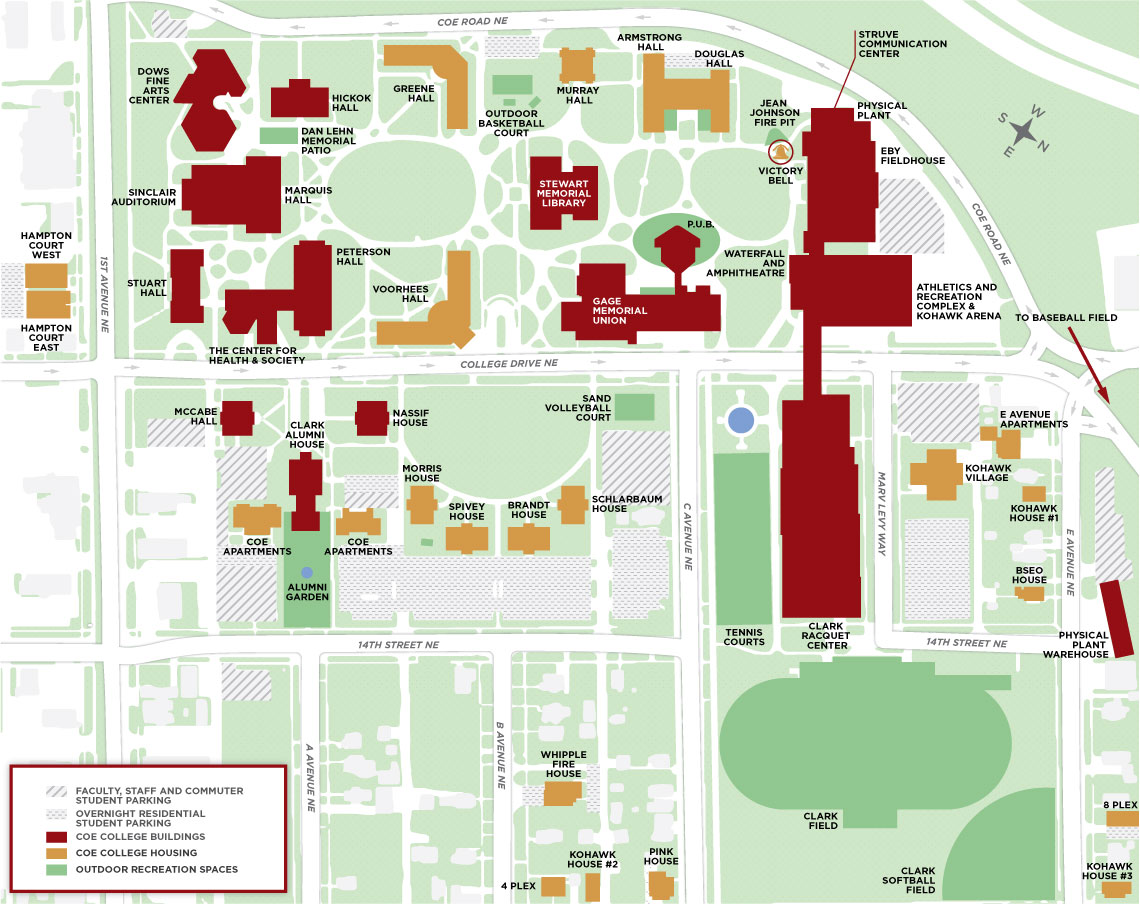
\includegraphics{catalog_sections/graphics/Campus-Map_full-screen.jpg}
\end{center}

\backmatter
\printindex

\end{document}
